\documentclass[a4paper, 12pt]{scrartcl}

% Most of the preamble is in here.
\usepackage[clearsection]{atureport}

% Heading
\title{Denoising Data Signals with\\[2mm] Fast Fourier Transforms using Python}
\subtitle{Individual Project Report for\\[2mm] MATH09101: Maths and Comp Modelling}
\author{Abdul Fatah Jamro {\Large (G00425616})}
\date{\today}


\begin{document}
  
\maketitle

\newpage

\section*{}
Thanks to my supervisor Dr Ian McLoughlin for help in editing and formatting this report and the associated work.

\tableofcontents

\newpage

\section{Introduction}

Noise is a major concern for scientists and engineers investigating data signals.
Techniques, such as shields and other denoising techniques, are typically used to protect signals and avoid noise.
To date, the Fast Fourier Transform (FFT)\footnote{Technically, there are several different Fast Fourier Transform algorithms.} has remained one of the best approaches to denoise, compress, or analyse data.
In the field of signal processing, noise removal is a basic problem where the FFT is used.

Computational tools enable the FFT to be used efficiently on most signals of reasonable size.
In this report, Python is used to apply a Fast Fourier transform in denoising a noisy audio signal.
In the following sections, we briefly explain Fourier series, the Fourier transform, and the Fast Fourier transform.
We follow this with example code written in Python. 

\subsection{Fourier Series}
A wave form or any periodic function can be represented as a Fourier series.
A Fourier series is a sum of sines or cosines waves.
The Fourier series is named after the French mathematician and scientist Jean-Baptiste Joseph Fourier (1768--1830).

Fourier transforms are frequently utilized in signal processing because sine waves are the building blocks of sound waves~\cite{tolstov1976fourier}.
Complex waves, like sound, can be decomposed as a combination of sine waves using a Fourier series.
A Fourier transform is a technique for separating a signal into its various frequencies~\cite{tolstov1976fourier}.
The series adds together the underlying sines or cosines waves of the signal.

This implies that a wave's constituent parts can be separated from one another.
The study of various Fourier series falls within the category of Fourier analysis.
In audio processing, such as when isolating specific sounds from a recording, Fourier analysis is frequently utilized~\cite{tolstov1976fourier}.

\subsection{Fourier Transform}
The Fourier transform (FT) uses signals based on time as its input to calculate the strength, rotation speed, and total cycle offset for each potential cycle.
Waveforms, having a function of time, space, or another variable, are subjected to the Fourier transform.
The Fourier transform represents any signal into sinusoid form.

A time function waveform is broken down into its constituent frequency function using the Fourier transform mathematical function.
The Fourier transform generates a complex valued function of frequency as its output.
While the Fourier transform's complex argument indicates the phase offset of the fundamental sinusoidal in that frequency, its absolute value represents the frequency value present in the original function.

The term Fourier Transform is often used to describe both the mathematical operation and the representation of the signal in the frequency domain.
It is considered a generalization of the Fourier series in which the concepts behind Fourier series can be applied to non-periodic signals.

The Fourier Transform (FT) of a function $f(x)$ is given in Equation \ref{eqn:FT} and its inverse is given in Equation \ref{eqn:InvFT}.

\begin{equation}
  \label{eqn:FT}
  F(k) = \int^{\infty}_{-\infty} f(x) e^{-2 \pi i k x} \,dx
\end{equation}

\begin{equation}
  \label{eqn:InvFT}
  f(x) = \int^{\infty}_{-\infty} F(k) e^{2 \pi i k x} \,dk
\end{equation}

We note here several interesting properties of the Fourier Transform.
\begin{description}
  \item[Linear transform:] if $g(t)$ and $h(t)$ are two Fourier transforms given by $G(f)$ and $H(f)$ respectively, then the Fourier transform of the linear combination of $g$ and $t$ can be easily calculated.
  \item[Time shift property:] the Fourier transform of $g(t - a)$ where a is a real number that shifts the original function has the same amount of shift in the magnitude of the spectrum.
  \item[Modulation property:] a function is modulated by another function when it is multiplied in time.
  \item[Parseval's theorem:] the Fourier transform is unitary, i.e., the sum of square of a function $g(t)$ equals the sum of the square of its Fourier transform, $G(f)$.
  \item[Duality:] the Fourier transform of $G(t)$ is $g$ if $g(t)$ possesses the Fourier transform $G(f) (-f)$.
\end{description}


\section{Fast Fourier Transform (FFT)}

The Discrete Fourier Transform (DFT) converts discrete time-based signals into discrete frequency-based signals.
The naive DFT algorithm is computationally complex but algorithms have been developed to compute it which are much more efficient~\cite{FFT}.
These are generally referred to as Fast Fourier Transforms (FFT's).
Thus, a Fast Fourier Transform algorithm calculates the Discrete Fourier Transform of a sequence.

The Discrete Fourier Transform converts a waveform's cycle structure into sine components.
Fast Fourier Transforms are used in many different signal processing techniques, such as image-processing and reading sound waves.
They can be used to quickly solve different kinds of equations or display different kinds of frequency activity.

The FFT and DFT are exceedingly technical aspects of both computing and electrical engineering.
They are mostly the domain of engineers and mathematicians attempting to alter or build components of various technologies.
For example, Fast Fourier Transform might be helpful in sound engineering, seismology, or in voltage measurements.
The FFT is a crucial measurement technique in the study of measuring audio and acoustics.
It breaks down a signal into its distinct spectral components, giving frequency information about the signal in the process.

FFT's are used for machine or system condition monitoring, quality control, and fault analysis.
This page covers the operation of an FFT, the pertinent parameters, and how they affect the measurement outcome.

Using an FFT, a signal is separated into its frequency components after being sampled over time.
Each of these elements is a discrete sinusoidal oscillation with a unique frequency, amplitude, and phase.
Figure \ref{fig:fourier} demonstrates the transformation.

\subsection{Formulas}

The Discrete Fourier Transform formula given in Equation \ref{eqn:dft} and it's inverse is given in Equation \ref{eqn:invdft}.
In the former, a discrete time-domain signal of length $N$ is transformed to a discrete frequency-domain signal of the same length.

\begin{equation}
  \label{eqn:dft}
  X_k = \sum_{n=0}^{N-1} x_n e^{-2 \pi i k n / N}
\end{equation}

\begin{equation}
  \label{eqn:invdft}
  x_n = \sum_{k=0}^{N-1} X_k e^{2 \pi i k n / N}
\end{equation}

 
In the frequency domain, data can be easily manipulated to, for instance, remove noise or apply data compression.
Then, we can revert the manipulated frequency domain signal to the time domain by the inverse operation.

\subsection{Visualization}

Figure \ref{fig:fourier} illustrates the Fourier Transform (FT): decomposition of a sophisticated wave into different sinusoidal waves.
\begin{figure}[H] 
  \centering
  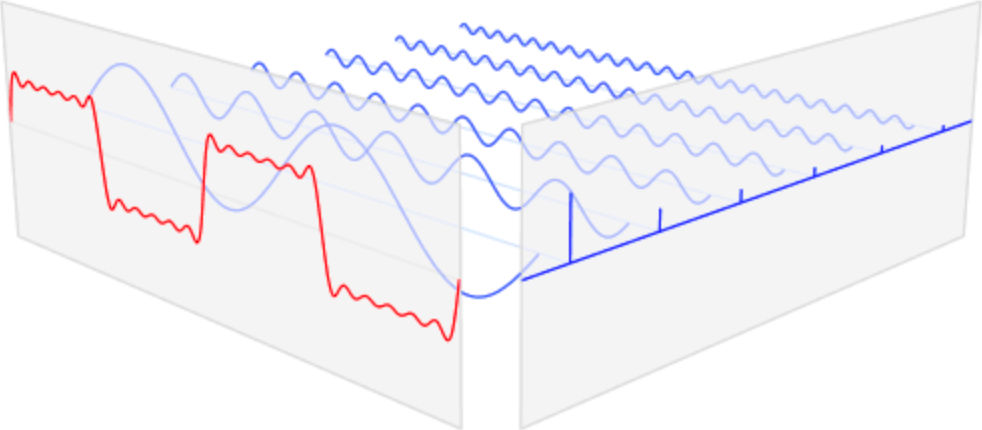
\includegraphics[width=0.6\textwidth]{img/fourier-dimensions.png}
  \caption{Frequency and time domains of a signal. (Image source wikipedia)}
  \label{fig:fourier}
\end{figure}
The wave function in red is the sum of the six waves shown in blue.
The Fourier Transform reveals the amplitudes of the summed sine waves.
Each bar on right side of the image shows a different frequency.  

\section{Practical Example: Denoising Audio Signals}
Let us put aside for the time being the difficulty of the Fourier Transform equations.
Let us pretend that we fully get the meaning of the mathematical equations and apply the Fourier Transform to carry out some useful work in Python~\cite{CleanUpNoise}.

We create two audio signals of different frequencies with the help of Python.
Plots of the individual signals are shown in Figures~\ref{fig:sixty} and \ref{fig:onefifty}.
We then combine them into a single resultant signal through addition.
We call this the clean signal as shown in Figure~\ref{fig:sumsignals}.

Both signals are in the time-domain, as time is on the $x$ axis.
The resultant signal is thus also in the time domain.
\subsection{Generating of two signals and their convolution sum with random noise}
\begin{figure}[H] 
  \centering
  \resizebox{\textwidth}{!}{%% Creator: Matplotlib, PGF backend
%%
%% To include the figure in your LaTeX document, write
%%   \input{<filename>.pgf}
%%
%% Make sure the required packages are loaded in your preamble
%%   \usepackage{pgf}
%%
%% Also ensure that all the required font packages are loaded; for instance,
%% the lmodern package is sometimes necessary when using math font.
%%   \usepackage{lmodern}
%%
%% Figures using additional raster images can only be included by \input if
%% they are in the same directory as the main LaTeX file. For loading figures
%% from other directories you can use the `import` package
%%   \usepackage{import}
%%
%% and then include the figures with
%%   \import{<path to file>}{<filename>.pgf}
%%
%% Matplotlib used the following preamble
%%   
%%   \usepackage{fontspec}
%%   \setmainfont{DejaVuSerif.ttf}[Path=\detokenize{/Users/ianmcloughlin/.miniconda3/lib/python3.9/site-packages/matplotlib/mpl-data/fonts/ttf/}]
%%   \setsansfont{DejaVuSans.ttf}[Path=\detokenize{/Users/ianmcloughlin/.miniconda3/lib/python3.9/site-packages/matplotlib/mpl-data/fonts/ttf/}]
%%   \setmonofont{DejaVuSansMono.ttf}[Path=\detokenize{/Users/ianmcloughlin/.miniconda3/lib/python3.9/site-packages/matplotlib/mpl-data/fonts/ttf/}]
%%   \makeatletter\@ifpackageloaded{underscore}{}{\usepackage[strings]{underscore}}\makeatother
%%
\begingroup%
\makeatletter%
\begin{pgfpicture}%
\pgfpathrectangle{\pgfpointorigin}{\pgfqpoint{12.000000in}{3.000000in}}%
\pgfusepath{use as bounding box, clip}%
\begin{pgfscope}%
\pgfsetbuttcap%
\pgfsetmiterjoin%
\definecolor{currentfill}{rgb}{1.000000,1.000000,1.000000}%
\pgfsetfillcolor{currentfill}%
\pgfsetlinewidth{0.000000pt}%
\definecolor{currentstroke}{rgb}{1.000000,1.000000,1.000000}%
\pgfsetstrokecolor{currentstroke}%
\pgfsetdash{}{0pt}%
\pgfpathmoveto{\pgfqpoint{0.000000in}{0.000000in}}%
\pgfpathlineto{\pgfqpoint{12.000000in}{0.000000in}}%
\pgfpathlineto{\pgfqpoint{12.000000in}{3.000000in}}%
\pgfpathlineto{\pgfqpoint{0.000000in}{3.000000in}}%
\pgfpathlineto{\pgfqpoint{0.000000in}{0.000000in}}%
\pgfpathclose%
\pgfusepath{fill}%
\end{pgfscope}%
\begin{pgfscope}%
\pgfsetbuttcap%
\pgfsetmiterjoin%
\definecolor{currentfill}{rgb}{1.000000,1.000000,1.000000}%
\pgfsetfillcolor{currentfill}%
\pgfsetlinewidth{0.000000pt}%
\definecolor{currentstroke}{rgb}{0.000000,0.000000,0.000000}%
\pgfsetstrokecolor{currentstroke}%
\pgfsetstrokeopacity{0.000000}%
\pgfsetdash{}{0pt}%
\pgfpathmoveto{\pgfqpoint{0.584722in}{0.582778in}}%
\pgfpathlineto{\pgfqpoint{11.850000in}{0.582778in}}%
\pgfpathlineto{\pgfqpoint{11.850000in}{2.850000in}}%
\pgfpathlineto{\pgfqpoint{0.584722in}{2.850000in}}%
\pgfpathlineto{\pgfqpoint{0.584722in}{0.582778in}}%
\pgfpathclose%
\pgfusepath{fill}%
\end{pgfscope}%
\begin{pgfscope}%
\pgfsetbuttcap%
\pgfsetroundjoin%
\definecolor{currentfill}{rgb}{0.000000,0.000000,0.000000}%
\pgfsetfillcolor{currentfill}%
\pgfsetlinewidth{0.803000pt}%
\definecolor{currentstroke}{rgb}{0.000000,0.000000,0.000000}%
\pgfsetstrokecolor{currentstroke}%
\pgfsetdash{}{0pt}%
\pgfsys@defobject{currentmarker}{\pgfqpoint{0.000000in}{-0.048611in}}{\pgfqpoint{0.000000in}{0.000000in}}{%
\pgfpathmoveto{\pgfqpoint{0.000000in}{0.000000in}}%
\pgfpathlineto{\pgfqpoint{0.000000in}{-0.048611in}}%
\pgfusepath{stroke,fill}%
}%
\begin{pgfscope}%
\pgfsys@transformshift{1.096780in}{0.582778in}%
\pgfsys@useobject{currentmarker}{}%
\end{pgfscope}%
\end{pgfscope}%
\begin{pgfscope}%
\definecolor{textcolor}{rgb}{0.000000,0.000000,0.000000}%
\pgfsetstrokecolor{textcolor}%
\pgfsetfillcolor{textcolor}%
\pgftext[x=1.096780in,y=0.485556in,,top]{\color{textcolor}\sffamily\fontsize{10.000000}{12.000000}\selectfont 0.00}%
\end{pgfscope}%
\begin{pgfscope}%
\pgfsetbuttcap%
\pgfsetroundjoin%
\definecolor{currentfill}{rgb}{0.000000,0.000000,0.000000}%
\pgfsetfillcolor{currentfill}%
\pgfsetlinewidth{0.803000pt}%
\definecolor{currentstroke}{rgb}{0.000000,0.000000,0.000000}%
\pgfsetstrokecolor{currentstroke}%
\pgfsetdash{}{0pt}%
\pgfsys@defobject{currentmarker}{\pgfqpoint{0.000000in}{-0.048611in}}{\pgfqpoint{0.000000in}{0.000000in}}{%
\pgfpathmoveto{\pgfqpoint{0.000000in}{0.000000in}}%
\pgfpathlineto{\pgfqpoint{0.000000in}{-0.048611in}}%
\pgfusepath{stroke,fill}%
}%
\begin{pgfscope}%
\pgfsys@transformshift{3.147063in}{0.582778in}%
\pgfsys@useobject{currentmarker}{}%
\end{pgfscope}%
\end{pgfscope}%
\begin{pgfscope}%
\definecolor{textcolor}{rgb}{0.000000,0.000000,0.000000}%
\pgfsetstrokecolor{textcolor}%
\pgfsetfillcolor{textcolor}%
\pgftext[x=3.147063in,y=0.485556in,,top]{\color{textcolor}\sffamily\fontsize{10.000000}{12.000000}\selectfont 0.02}%
\end{pgfscope}%
\begin{pgfscope}%
\pgfsetbuttcap%
\pgfsetroundjoin%
\definecolor{currentfill}{rgb}{0.000000,0.000000,0.000000}%
\pgfsetfillcolor{currentfill}%
\pgfsetlinewidth{0.803000pt}%
\definecolor{currentstroke}{rgb}{0.000000,0.000000,0.000000}%
\pgfsetstrokecolor{currentstroke}%
\pgfsetdash{}{0pt}%
\pgfsys@defobject{currentmarker}{\pgfqpoint{0.000000in}{-0.048611in}}{\pgfqpoint{0.000000in}{0.000000in}}{%
\pgfpathmoveto{\pgfqpoint{0.000000in}{0.000000in}}%
\pgfpathlineto{\pgfqpoint{0.000000in}{-0.048611in}}%
\pgfusepath{stroke,fill}%
}%
\begin{pgfscope}%
\pgfsys@transformshift{5.197346in}{0.582778in}%
\pgfsys@useobject{currentmarker}{}%
\end{pgfscope}%
\end{pgfscope}%
\begin{pgfscope}%
\definecolor{textcolor}{rgb}{0.000000,0.000000,0.000000}%
\pgfsetstrokecolor{textcolor}%
\pgfsetfillcolor{textcolor}%
\pgftext[x=5.197346in,y=0.485556in,,top]{\color{textcolor}\sffamily\fontsize{10.000000}{12.000000}\selectfont 0.04}%
\end{pgfscope}%
\begin{pgfscope}%
\pgfsetbuttcap%
\pgfsetroundjoin%
\definecolor{currentfill}{rgb}{0.000000,0.000000,0.000000}%
\pgfsetfillcolor{currentfill}%
\pgfsetlinewidth{0.803000pt}%
\definecolor{currentstroke}{rgb}{0.000000,0.000000,0.000000}%
\pgfsetstrokecolor{currentstroke}%
\pgfsetdash{}{0pt}%
\pgfsys@defobject{currentmarker}{\pgfqpoint{0.000000in}{-0.048611in}}{\pgfqpoint{0.000000in}{0.000000in}}{%
\pgfpathmoveto{\pgfqpoint{0.000000in}{0.000000in}}%
\pgfpathlineto{\pgfqpoint{0.000000in}{-0.048611in}}%
\pgfusepath{stroke,fill}%
}%
\begin{pgfscope}%
\pgfsys@transformshift{7.247628in}{0.582778in}%
\pgfsys@useobject{currentmarker}{}%
\end{pgfscope}%
\end{pgfscope}%
\begin{pgfscope}%
\definecolor{textcolor}{rgb}{0.000000,0.000000,0.000000}%
\pgfsetstrokecolor{textcolor}%
\pgfsetfillcolor{textcolor}%
\pgftext[x=7.247628in,y=0.485556in,,top]{\color{textcolor}\sffamily\fontsize{10.000000}{12.000000}\selectfont 0.06}%
\end{pgfscope}%
\begin{pgfscope}%
\pgfsetbuttcap%
\pgfsetroundjoin%
\definecolor{currentfill}{rgb}{0.000000,0.000000,0.000000}%
\pgfsetfillcolor{currentfill}%
\pgfsetlinewidth{0.803000pt}%
\definecolor{currentstroke}{rgb}{0.000000,0.000000,0.000000}%
\pgfsetstrokecolor{currentstroke}%
\pgfsetdash{}{0pt}%
\pgfsys@defobject{currentmarker}{\pgfqpoint{0.000000in}{-0.048611in}}{\pgfqpoint{0.000000in}{0.000000in}}{%
\pgfpathmoveto{\pgfqpoint{0.000000in}{0.000000in}}%
\pgfpathlineto{\pgfqpoint{0.000000in}{-0.048611in}}%
\pgfusepath{stroke,fill}%
}%
\begin{pgfscope}%
\pgfsys@transformshift{9.297911in}{0.582778in}%
\pgfsys@useobject{currentmarker}{}%
\end{pgfscope}%
\end{pgfscope}%
\begin{pgfscope}%
\definecolor{textcolor}{rgb}{0.000000,0.000000,0.000000}%
\pgfsetstrokecolor{textcolor}%
\pgfsetfillcolor{textcolor}%
\pgftext[x=9.297911in,y=0.485556in,,top]{\color{textcolor}\sffamily\fontsize{10.000000}{12.000000}\selectfont 0.08}%
\end{pgfscope}%
\begin{pgfscope}%
\pgfsetbuttcap%
\pgfsetroundjoin%
\definecolor{currentfill}{rgb}{0.000000,0.000000,0.000000}%
\pgfsetfillcolor{currentfill}%
\pgfsetlinewidth{0.803000pt}%
\definecolor{currentstroke}{rgb}{0.000000,0.000000,0.000000}%
\pgfsetstrokecolor{currentstroke}%
\pgfsetdash{}{0pt}%
\pgfsys@defobject{currentmarker}{\pgfqpoint{0.000000in}{-0.048611in}}{\pgfqpoint{0.000000in}{0.000000in}}{%
\pgfpathmoveto{\pgfqpoint{0.000000in}{0.000000in}}%
\pgfpathlineto{\pgfqpoint{0.000000in}{-0.048611in}}%
\pgfusepath{stroke,fill}%
}%
\begin{pgfscope}%
\pgfsys@transformshift{11.348193in}{0.582778in}%
\pgfsys@useobject{currentmarker}{}%
\end{pgfscope}%
\end{pgfscope}%
\begin{pgfscope}%
\definecolor{textcolor}{rgb}{0.000000,0.000000,0.000000}%
\pgfsetstrokecolor{textcolor}%
\pgfsetfillcolor{textcolor}%
\pgftext[x=11.348193in,y=0.485556in,,top]{\color{textcolor}\sffamily\fontsize{10.000000}{12.000000}\selectfont 0.10}%
\end{pgfscope}%
\begin{pgfscope}%
\definecolor{textcolor}{rgb}{0.000000,0.000000,0.000000}%
\pgfsetstrokecolor{textcolor}%
\pgfsetfillcolor{textcolor}%
\pgftext[x=6.217361in,y=0.295587in,,top]{\color{textcolor}\sffamily\fontsize{10.000000}{12.000000}\selectfont Time}%
\end{pgfscope}%
\begin{pgfscope}%
\pgfsetbuttcap%
\pgfsetroundjoin%
\definecolor{currentfill}{rgb}{0.000000,0.000000,0.000000}%
\pgfsetfillcolor{currentfill}%
\pgfsetlinewidth{0.803000pt}%
\definecolor{currentstroke}{rgb}{0.000000,0.000000,0.000000}%
\pgfsetstrokecolor{currentstroke}%
\pgfsetdash{}{0pt}%
\pgfsys@defobject{currentmarker}{\pgfqpoint{-0.048611in}{0.000000in}}{\pgfqpoint{-0.000000in}{0.000000in}}{%
\pgfpathmoveto{\pgfqpoint{-0.000000in}{0.000000in}}%
\pgfpathlineto{\pgfqpoint{-0.048611in}{0.000000in}}%
\pgfusepath{stroke,fill}%
}%
\begin{pgfscope}%
\pgfsys@transformshift{0.584722in}{0.685833in}%
\pgfsys@useobject{currentmarker}{}%
\end{pgfscope}%
\end{pgfscope}%
\begin{pgfscope}%
\definecolor{textcolor}{rgb}{0.000000,0.000000,0.000000}%
\pgfsetstrokecolor{textcolor}%
\pgfsetfillcolor{textcolor}%
\pgftext[x=0.158596in, y=0.633072in, left, base]{\color{textcolor}\sffamily\fontsize{10.000000}{12.000000}\selectfont \ensuremath{-}1.0}%
\end{pgfscope}%
\begin{pgfscope}%
\pgfsetbuttcap%
\pgfsetroundjoin%
\definecolor{currentfill}{rgb}{0.000000,0.000000,0.000000}%
\pgfsetfillcolor{currentfill}%
\pgfsetlinewidth{0.803000pt}%
\definecolor{currentstroke}{rgb}{0.000000,0.000000,0.000000}%
\pgfsetstrokecolor{currentstroke}%
\pgfsetdash{}{0pt}%
\pgfsys@defobject{currentmarker}{\pgfqpoint{-0.048611in}{0.000000in}}{\pgfqpoint{-0.000000in}{0.000000in}}{%
\pgfpathmoveto{\pgfqpoint{-0.000000in}{0.000000in}}%
\pgfpathlineto{\pgfqpoint{-0.048611in}{0.000000in}}%
\pgfusepath{stroke,fill}%
}%
\begin{pgfscope}%
\pgfsys@transformshift{0.584722in}{1.201111in}%
\pgfsys@useobject{currentmarker}{}%
\end{pgfscope}%
\end{pgfscope}%
\begin{pgfscope}%
\definecolor{textcolor}{rgb}{0.000000,0.000000,0.000000}%
\pgfsetstrokecolor{textcolor}%
\pgfsetfillcolor{textcolor}%
\pgftext[x=0.158596in, y=1.148350in, left, base]{\color{textcolor}\sffamily\fontsize{10.000000}{12.000000}\selectfont \ensuremath{-}0.5}%
\end{pgfscope}%
\begin{pgfscope}%
\pgfsetbuttcap%
\pgfsetroundjoin%
\definecolor{currentfill}{rgb}{0.000000,0.000000,0.000000}%
\pgfsetfillcolor{currentfill}%
\pgfsetlinewidth{0.803000pt}%
\definecolor{currentstroke}{rgb}{0.000000,0.000000,0.000000}%
\pgfsetstrokecolor{currentstroke}%
\pgfsetdash{}{0pt}%
\pgfsys@defobject{currentmarker}{\pgfqpoint{-0.048611in}{0.000000in}}{\pgfqpoint{-0.000000in}{0.000000in}}{%
\pgfpathmoveto{\pgfqpoint{-0.000000in}{0.000000in}}%
\pgfpathlineto{\pgfqpoint{-0.048611in}{0.000000in}}%
\pgfusepath{stroke,fill}%
}%
\begin{pgfscope}%
\pgfsys@transformshift{0.584722in}{1.716389in}%
\pgfsys@useobject{currentmarker}{}%
\end{pgfscope}%
\end{pgfscope}%
\begin{pgfscope}%
\definecolor{textcolor}{rgb}{0.000000,0.000000,0.000000}%
\pgfsetstrokecolor{textcolor}%
\pgfsetfillcolor{textcolor}%
\pgftext[x=0.266621in, y=1.663627in, left, base]{\color{textcolor}\sffamily\fontsize{10.000000}{12.000000}\selectfont 0.0}%
\end{pgfscope}%
\begin{pgfscope}%
\pgfsetbuttcap%
\pgfsetroundjoin%
\definecolor{currentfill}{rgb}{0.000000,0.000000,0.000000}%
\pgfsetfillcolor{currentfill}%
\pgfsetlinewidth{0.803000pt}%
\definecolor{currentstroke}{rgb}{0.000000,0.000000,0.000000}%
\pgfsetstrokecolor{currentstroke}%
\pgfsetdash{}{0pt}%
\pgfsys@defobject{currentmarker}{\pgfqpoint{-0.048611in}{0.000000in}}{\pgfqpoint{-0.000000in}{0.000000in}}{%
\pgfpathmoveto{\pgfqpoint{-0.000000in}{0.000000in}}%
\pgfpathlineto{\pgfqpoint{-0.048611in}{0.000000in}}%
\pgfusepath{stroke,fill}%
}%
\begin{pgfscope}%
\pgfsys@transformshift{0.584722in}{2.231667in}%
\pgfsys@useobject{currentmarker}{}%
\end{pgfscope}%
\end{pgfscope}%
\begin{pgfscope}%
\definecolor{textcolor}{rgb}{0.000000,0.000000,0.000000}%
\pgfsetstrokecolor{textcolor}%
\pgfsetfillcolor{textcolor}%
\pgftext[x=0.266621in, y=2.178905in, left, base]{\color{textcolor}\sffamily\fontsize{10.000000}{12.000000}\selectfont 0.5}%
\end{pgfscope}%
\begin{pgfscope}%
\pgfsetbuttcap%
\pgfsetroundjoin%
\definecolor{currentfill}{rgb}{0.000000,0.000000,0.000000}%
\pgfsetfillcolor{currentfill}%
\pgfsetlinewidth{0.803000pt}%
\definecolor{currentstroke}{rgb}{0.000000,0.000000,0.000000}%
\pgfsetstrokecolor{currentstroke}%
\pgfsetdash{}{0pt}%
\pgfsys@defobject{currentmarker}{\pgfqpoint{-0.048611in}{0.000000in}}{\pgfqpoint{-0.000000in}{0.000000in}}{%
\pgfpathmoveto{\pgfqpoint{-0.000000in}{0.000000in}}%
\pgfpathlineto{\pgfqpoint{-0.048611in}{0.000000in}}%
\pgfusepath{stroke,fill}%
}%
\begin{pgfscope}%
\pgfsys@transformshift{0.584722in}{2.746944in}%
\pgfsys@useobject{currentmarker}{}%
\end{pgfscope}%
\end{pgfscope}%
\begin{pgfscope}%
\definecolor{textcolor}{rgb}{0.000000,0.000000,0.000000}%
\pgfsetstrokecolor{textcolor}%
\pgfsetfillcolor{textcolor}%
\pgftext[x=0.266621in, y=2.694183in, left, base]{\color{textcolor}\sffamily\fontsize{10.000000}{12.000000}\selectfont 1.0}%
\end{pgfscope}%
\begin{pgfscope}%
\pgfpathrectangle{\pgfqpoint{0.584722in}{0.582778in}}{\pgfqpoint{11.265278in}{2.267222in}}%
\pgfusepath{clip}%
\pgfsetrectcap%
\pgfsetroundjoin%
\pgfsetlinewidth{1.505625pt}%
\definecolor{currentstroke}{rgb}{0.000000,0.356863,0.368627}%
\pgfsetstrokecolor{currentstroke}%
\pgfsetdash{}{0pt}%
\pgfpathmoveto{\pgfqpoint{1.096780in}{1.716389in}}%
\pgfpathlineto{\pgfqpoint{1.168540in}{1.985201in}}%
\pgfpathlineto{\pgfqpoint{1.209546in}{2.131606in}}%
\pgfpathlineto{\pgfqpoint{1.240300in}{2.235401in}}%
\pgfpathlineto{\pgfqpoint{1.271054in}{2.332563in}}%
\pgfpathlineto{\pgfqpoint{1.301809in}{2.421853in}}%
\pgfpathlineto{\pgfqpoint{1.332563in}{2.502128in}}%
\pgfpathlineto{\pgfqpoint{1.353066in}{2.550126in}}%
\pgfpathlineto{\pgfqpoint{1.373568in}{2.593386in}}%
\pgfpathlineto{\pgfqpoint{1.394071in}{2.631663in}}%
\pgfpathlineto{\pgfqpoint{1.414574in}{2.664739in}}%
\pgfpathlineto{\pgfqpoint{1.435077in}{2.692426in}}%
\pgfpathlineto{\pgfqpoint{1.455580in}{2.714568in}}%
\pgfpathlineto{\pgfqpoint{1.476083in}{2.731037in}}%
\pgfpathlineto{\pgfqpoint{1.486334in}{2.737114in}}%
\pgfpathlineto{\pgfqpoint{1.496585in}{2.741741in}}%
\pgfpathlineto{\pgfqpoint{1.506837in}{2.744911in}}%
\pgfpathlineto{\pgfqpoint{1.517088in}{2.746619in}}%
\pgfpathlineto{\pgfqpoint{1.527340in}{2.746863in}}%
\pgfpathlineto{\pgfqpoint{1.537591in}{2.745643in}}%
\pgfpathlineto{\pgfqpoint{1.547842in}{2.742960in}}%
\pgfpathlineto{\pgfqpoint{1.558094in}{2.738818in}}%
\pgfpathlineto{\pgfqpoint{1.568345in}{2.733224in}}%
\pgfpathlineto{\pgfqpoint{1.578597in}{2.726184in}}%
\pgfpathlineto{\pgfqpoint{1.599100in}{2.707812in}}%
\pgfpathlineto{\pgfqpoint{1.619602in}{2.683806in}}%
\pgfpathlineto{\pgfqpoint{1.640105in}{2.654304in}}%
\pgfpathlineto{\pgfqpoint{1.660608in}{2.619472in}}%
\pgfpathlineto{\pgfqpoint{1.681111in}{2.579508in}}%
\pgfpathlineto{\pgfqpoint{1.701614in}{2.534640in}}%
\pgfpathlineto{\pgfqpoint{1.722116in}{2.485123in}}%
\pgfpathlineto{\pgfqpoint{1.742619in}{2.431237in}}%
\pgfpathlineto{\pgfqpoint{1.773374in}{2.342895in}}%
\pgfpathlineto{\pgfqpoint{1.804128in}{2.246547in}}%
\pgfpathlineto{\pgfqpoint{1.834882in}{2.143426in}}%
\pgfpathlineto{\pgfqpoint{1.875888in}{1.997681in}}%
\pgfpathlineto{\pgfqpoint{1.937396in}{1.768168in}}%
\pgfpathlineto{\pgfqpoint{2.029659in}{1.422661in}}%
\pgfpathlineto{\pgfqpoint{2.070665in}{1.277600in}}%
\pgfpathlineto{\pgfqpoint{2.101419in}{1.175167in}}%
\pgfpathlineto{\pgfqpoint{2.132173in}{1.079650in}}%
\pgfpathlineto{\pgfqpoint{2.162927in}{0.992269in}}%
\pgfpathlineto{\pgfqpoint{2.183430in}{0.939091in}}%
\pgfpathlineto{\pgfqpoint{2.203933in}{0.890330in}}%
\pgfpathlineto{\pgfqpoint{2.224436in}{0.846262in}}%
\pgfpathlineto{\pgfqpoint{2.244939in}{0.807139in}}%
\pgfpathlineto{\pgfqpoint{2.265441in}{0.773182in}}%
\pgfpathlineto{\pgfqpoint{2.285944in}{0.744585in}}%
\pgfpathlineto{\pgfqpoint{2.306447in}{0.721509in}}%
\pgfpathlineto{\pgfqpoint{2.326950in}{0.704087in}}%
\pgfpathlineto{\pgfqpoint{2.337201in}{0.697528in}}%
\pgfpathlineto{\pgfqpoint{2.347453in}{0.692417in}}%
\pgfpathlineto{\pgfqpoint{2.357704in}{0.688761in}}%
\pgfpathlineto{\pgfqpoint{2.367956in}{0.686566in}}%
\pgfpathlineto{\pgfqpoint{2.378207in}{0.685833in}}%
\pgfpathlineto{\pgfqpoint{2.388458in}{0.686566in}}%
\pgfpathlineto{\pgfqpoint{2.398710in}{0.688761in}}%
\pgfpathlineto{\pgfqpoint{2.408961in}{0.692417in}}%
\pgfpathlineto{\pgfqpoint{2.419213in}{0.697528in}}%
\pgfpathlineto{\pgfqpoint{2.429464in}{0.704087in}}%
\pgfpathlineto{\pgfqpoint{2.439715in}{0.712085in}}%
\pgfpathlineto{\pgfqpoint{2.460218in}{0.732348in}}%
\pgfpathlineto{\pgfqpoint{2.480721in}{0.758203in}}%
\pgfpathlineto{\pgfqpoint{2.501224in}{0.789502in}}%
\pgfpathlineto{\pgfqpoint{2.521727in}{0.826068in}}%
\pgfpathlineto{\pgfqpoint{2.542230in}{0.867693in}}%
\pgfpathlineto{\pgfqpoint{2.562732in}{0.914140in}}%
\pgfpathlineto{\pgfqpoint{2.583235in}{0.965146in}}%
\pgfpathlineto{\pgfqpoint{2.613989in}{1.049562in}}%
\pgfpathlineto{\pgfqpoint{2.644744in}{1.142498in}}%
\pgfpathlineto{\pgfqpoint{2.675498in}{1.242766in}}%
\pgfpathlineto{\pgfqpoint{2.716504in}{1.385639in}}%
\pgfpathlineto{\pgfqpoint{2.767761in}{1.574388in}}%
\pgfpathlineto{\pgfqpoint{2.901029in}{2.071563in}}%
\pgfpathlineto{\pgfqpoint{2.942035in}{2.212863in}}%
\pgfpathlineto{\pgfqpoint{2.972789in}{2.311610in}}%
\pgfpathlineto{\pgfqpoint{3.003543in}{2.402751in}}%
\pgfpathlineto{\pgfqpoint{3.034297in}{2.485123in}}%
\pgfpathlineto{\pgfqpoint{3.054800in}{2.534640in}}%
\pgfpathlineto{\pgfqpoint{3.075303in}{2.579508in}}%
\pgfpathlineto{\pgfqpoint{3.095806in}{2.619472in}}%
\pgfpathlineto{\pgfqpoint{3.116309in}{2.654304in}}%
\pgfpathlineto{\pgfqpoint{3.136811in}{2.683806in}}%
\pgfpathlineto{\pgfqpoint{3.157314in}{2.707812in}}%
\pgfpathlineto{\pgfqpoint{3.177817in}{2.726184in}}%
\pgfpathlineto{\pgfqpoint{3.188069in}{2.733224in}}%
\pgfpathlineto{\pgfqpoint{3.198320in}{2.738818in}}%
\pgfpathlineto{\pgfqpoint{3.208571in}{2.742960in}}%
\pgfpathlineto{\pgfqpoint{3.218823in}{2.745643in}}%
\pgfpathlineto{\pgfqpoint{3.229074in}{2.746863in}}%
\pgfpathlineto{\pgfqpoint{3.239326in}{2.746619in}}%
\pgfpathlineto{\pgfqpoint{3.249577in}{2.744911in}}%
\pgfpathlineto{\pgfqpoint{3.259828in}{2.741741in}}%
\pgfpathlineto{\pgfqpoint{3.270080in}{2.737114in}}%
\pgfpathlineto{\pgfqpoint{3.280331in}{2.731037in}}%
\pgfpathlineto{\pgfqpoint{3.290583in}{2.723518in}}%
\pgfpathlineto{\pgfqpoint{3.311086in}{2.704199in}}%
\pgfpathlineto{\pgfqpoint{3.331588in}{2.679267in}}%
\pgfpathlineto{\pgfqpoint{3.352091in}{2.648863in}}%
\pgfpathlineto{\pgfqpoint{3.372594in}{2.613162in}}%
\pgfpathlineto{\pgfqpoint{3.393097in}{2.572364in}}%
\pgfpathlineto{\pgfqpoint{3.413600in}{2.526703in}}%
\pgfpathlineto{\pgfqpoint{3.434102in}{2.476437in}}%
\pgfpathlineto{\pgfqpoint{3.464857in}{2.393037in}}%
\pgfpathlineto{\pgfqpoint{3.495611in}{2.300991in}}%
\pgfpathlineto{\pgfqpoint{3.526365in}{2.201475in}}%
\pgfpathlineto{\pgfqpoint{3.567371in}{2.059378in}}%
\pgfpathlineto{\pgfqpoint{3.618628in}{1.871205in}}%
\pgfpathlineto{\pgfqpoint{3.751896in}{1.373400in}}%
\pgfpathlineto{\pgfqpoint{3.792902in}{1.231302in}}%
\pgfpathlineto{\pgfqpoint{3.823656in}{1.131787in}}%
\pgfpathlineto{\pgfqpoint{3.854410in}{1.039741in}}%
\pgfpathlineto{\pgfqpoint{3.885165in}{0.956341in}}%
\pgfpathlineto{\pgfqpoint{3.905667in}{0.906075in}}%
\pgfpathlineto{\pgfqpoint{3.926170in}{0.860414in}}%
\pgfpathlineto{\pgfqpoint{3.946673in}{0.819616in}}%
\pgfpathlineto{\pgfqpoint{3.967176in}{0.783914in}}%
\pgfpathlineto{\pgfqpoint{3.987679in}{0.753511in}}%
\pgfpathlineto{\pgfqpoint{4.008182in}{0.728579in}}%
\pgfpathlineto{\pgfqpoint{4.028684in}{0.709260in}}%
\pgfpathlineto{\pgfqpoint{4.038936in}{0.701741in}}%
\pgfpathlineto{\pgfqpoint{4.049187in}{0.695663in}}%
\pgfpathlineto{\pgfqpoint{4.059439in}{0.691037in}}%
\pgfpathlineto{\pgfqpoint{4.069690in}{0.687867in}}%
\pgfpathlineto{\pgfqpoint{4.079941in}{0.686159in}}%
\pgfpathlineto{\pgfqpoint{4.090193in}{0.685915in}}%
\pgfpathlineto{\pgfqpoint{4.100444in}{0.687135in}}%
\pgfpathlineto{\pgfqpoint{4.110696in}{0.689818in}}%
\pgfpathlineto{\pgfqpoint{4.120947in}{0.693960in}}%
\pgfpathlineto{\pgfqpoint{4.131199in}{0.699554in}}%
\pgfpathlineto{\pgfqpoint{4.141450in}{0.706594in}}%
\pgfpathlineto{\pgfqpoint{4.161953in}{0.724966in}}%
\pgfpathlineto{\pgfqpoint{4.182456in}{0.748971in}}%
\pgfpathlineto{\pgfqpoint{4.202958in}{0.778474in}}%
\pgfpathlineto{\pgfqpoint{4.223461in}{0.813306in}}%
\pgfpathlineto{\pgfqpoint{4.243964in}{0.853270in}}%
\pgfpathlineto{\pgfqpoint{4.264467in}{0.898138in}}%
\pgfpathlineto{\pgfqpoint{4.284970in}{0.947655in}}%
\pgfpathlineto{\pgfqpoint{4.305473in}{1.001541in}}%
\pgfpathlineto{\pgfqpoint{4.336227in}{1.089883in}}%
\pgfpathlineto{\pgfqpoint{4.366981in}{1.186230in}}%
\pgfpathlineto{\pgfqpoint{4.397735in}{1.289352in}}%
\pgfpathlineto{\pgfqpoint{4.438741in}{1.435097in}}%
\pgfpathlineto{\pgfqpoint{4.500249in}{1.664609in}}%
\pgfpathlineto{\pgfqpoint{4.592512in}{2.010117in}}%
\pgfpathlineto{\pgfqpoint{4.633518in}{2.155178in}}%
\pgfpathlineto{\pgfqpoint{4.664272in}{2.257611in}}%
\pgfpathlineto{\pgfqpoint{4.695026in}{2.353128in}}%
\pgfpathlineto{\pgfqpoint{4.725781in}{2.440509in}}%
\pgfpathlineto{\pgfqpoint{4.746283in}{2.493687in}}%
\pgfpathlineto{\pgfqpoint{4.766786in}{2.542448in}}%
\pgfpathlineto{\pgfqpoint{4.787289in}{2.586516in}}%
\pgfpathlineto{\pgfqpoint{4.807792in}{2.625639in}}%
\pgfpathlineto{\pgfqpoint{4.828295in}{2.659596in}}%
\pgfpathlineto{\pgfqpoint{4.848797in}{2.688193in}}%
\pgfpathlineto{\pgfqpoint{4.869300in}{2.711268in}}%
\pgfpathlineto{\pgfqpoint{4.889803in}{2.728690in}}%
\pgfpathlineto{\pgfqpoint{4.900055in}{2.735249in}}%
\pgfpathlineto{\pgfqpoint{4.910306in}{2.740361in}}%
\pgfpathlineto{\pgfqpoint{4.920557in}{2.744017in}}%
\pgfpathlineto{\pgfqpoint{4.930809in}{2.746212in}}%
\pgfpathlineto{\pgfqpoint{4.941060in}{2.746944in}}%
\pgfpathlineto{\pgfqpoint{4.951312in}{2.746212in}}%
\pgfpathlineto{\pgfqpoint{4.961563in}{2.744017in}}%
\pgfpathlineto{\pgfqpoint{4.971814in}{2.740361in}}%
\pgfpathlineto{\pgfqpoint{4.982066in}{2.735249in}}%
\pgfpathlineto{\pgfqpoint{4.992317in}{2.728690in}}%
\pgfpathlineto{\pgfqpoint{5.002569in}{2.720693in}}%
\pgfpathlineto{\pgfqpoint{5.023071in}{2.700430in}}%
\pgfpathlineto{\pgfqpoint{5.043574in}{2.674575in}}%
\pgfpathlineto{\pgfqpoint{5.064077in}{2.643276in}}%
\pgfpathlineto{\pgfqpoint{5.084580in}{2.606710in}}%
\pgfpathlineto{\pgfqpoint{5.105083in}{2.565085in}}%
\pgfpathlineto{\pgfqpoint{5.125586in}{2.518638in}}%
\pgfpathlineto{\pgfqpoint{5.146088in}{2.467632in}}%
\pgfpathlineto{\pgfqpoint{5.176843in}{2.383216in}}%
\pgfpathlineto{\pgfqpoint{5.207597in}{2.290280in}}%
\pgfpathlineto{\pgfqpoint{5.238351in}{2.190011in}}%
\pgfpathlineto{\pgfqpoint{5.279357in}{2.047139in}}%
\pgfpathlineto{\pgfqpoint{5.330614in}{1.858389in}}%
\pgfpathlineto{\pgfqpoint{5.463882in}{1.361215in}}%
\pgfpathlineto{\pgfqpoint{5.504888in}{1.219915in}}%
\pgfpathlineto{\pgfqpoint{5.535642in}{1.121168in}}%
\pgfpathlineto{\pgfqpoint{5.566396in}{1.030027in}}%
\pgfpathlineto{\pgfqpoint{5.597151in}{0.947655in}}%
\pgfpathlineto{\pgfqpoint{5.617653in}{0.898138in}}%
\pgfpathlineto{\pgfqpoint{5.638156in}{0.853270in}}%
\pgfpathlineto{\pgfqpoint{5.658659in}{0.813306in}}%
\pgfpathlineto{\pgfqpoint{5.679162in}{0.778474in}}%
\pgfpathlineto{\pgfqpoint{5.699665in}{0.748971in}}%
\pgfpathlineto{\pgfqpoint{5.720168in}{0.724966in}}%
\pgfpathlineto{\pgfqpoint{5.740670in}{0.706594in}}%
\pgfpathlineto{\pgfqpoint{5.750922in}{0.699554in}}%
\pgfpathlineto{\pgfqpoint{5.761173in}{0.693960in}}%
\pgfpathlineto{\pgfqpoint{5.771425in}{0.689818in}}%
\pgfpathlineto{\pgfqpoint{5.781676in}{0.687135in}}%
\pgfpathlineto{\pgfqpoint{5.791927in}{0.685915in}}%
\pgfpathlineto{\pgfqpoint{5.802179in}{0.686159in}}%
\pgfpathlineto{\pgfqpoint{5.812430in}{0.687867in}}%
\pgfpathlineto{\pgfqpoint{5.822682in}{0.691037in}}%
\pgfpathlineto{\pgfqpoint{5.832933in}{0.695663in}}%
\pgfpathlineto{\pgfqpoint{5.843185in}{0.701741in}}%
\pgfpathlineto{\pgfqpoint{5.853436in}{0.709260in}}%
\pgfpathlineto{\pgfqpoint{5.873939in}{0.728579in}}%
\pgfpathlineto{\pgfqpoint{5.894442in}{0.753511in}}%
\pgfpathlineto{\pgfqpoint{5.914944in}{0.783914in}}%
\pgfpathlineto{\pgfqpoint{5.935447in}{0.819616in}}%
\pgfpathlineto{\pgfqpoint{5.955950in}{0.860414in}}%
\pgfpathlineto{\pgfqpoint{5.976453in}{0.906075in}}%
\pgfpathlineto{\pgfqpoint{5.996956in}{0.956341in}}%
\pgfpathlineto{\pgfqpoint{6.027710in}{1.039741in}}%
\pgfpathlineto{\pgfqpoint{6.058464in}{1.131787in}}%
\pgfpathlineto{\pgfqpoint{6.089218in}{1.231302in}}%
\pgfpathlineto{\pgfqpoint{6.130224in}{1.373400in}}%
\pgfpathlineto{\pgfqpoint{6.181481in}{1.561573in}}%
\pgfpathlineto{\pgfqpoint{6.314750in}{2.059378in}}%
\pgfpathlineto{\pgfqpoint{6.355755in}{2.201475in}}%
\pgfpathlineto{\pgfqpoint{6.386509in}{2.300991in}}%
\pgfpathlineto{\pgfqpoint{6.417264in}{2.393037in}}%
\pgfpathlineto{\pgfqpoint{6.448018in}{2.476437in}}%
\pgfpathlineto{\pgfqpoint{6.468521in}{2.526703in}}%
\pgfpathlineto{\pgfqpoint{6.489024in}{2.572364in}}%
\pgfpathlineto{\pgfqpoint{6.509526in}{2.613162in}}%
\pgfpathlineto{\pgfqpoint{6.530029in}{2.648863in}}%
\pgfpathlineto{\pgfqpoint{6.550532in}{2.679267in}}%
\pgfpathlineto{\pgfqpoint{6.571035in}{2.704199in}}%
\pgfpathlineto{\pgfqpoint{6.591538in}{2.723518in}}%
\pgfpathlineto{\pgfqpoint{6.601789in}{2.731037in}}%
\pgfpathlineto{\pgfqpoint{6.612041in}{2.737114in}}%
\pgfpathlineto{\pgfqpoint{6.622292in}{2.741741in}}%
\pgfpathlineto{\pgfqpoint{6.632543in}{2.744911in}}%
\pgfpathlineto{\pgfqpoint{6.642795in}{2.746619in}}%
\pgfpathlineto{\pgfqpoint{6.653046in}{2.746863in}}%
\pgfpathlineto{\pgfqpoint{6.663298in}{2.745643in}}%
\pgfpathlineto{\pgfqpoint{6.673549in}{2.742960in}}%
\pgfpathlineto{\pgfqpoint{6.683800in}{2.738818in}}%
\pgfpathlineto{\pgfqpoint{6.694052in}{2.733224in}}%
\pgfpathlineto{\pgfqpoint{6.704303in}{2.726184in}}%
\pgfpathlineto{\pgfqpoint{6.724806in}{2.707812in}}%
\pgfpathlineto{\pgfqpoint{6.745309in}{2.683806in}}%
\pgfpathlineto{\pgfqpoint{6.765812in}{2.654304in}}%
\pgfpathlineto{\pgfqpoint{6.786315in}{2.619472in}}%
\pgfpathlineto{\pgfqpoint{6.806817in}{2.579508in}}%
\pgfpathlineto{\pgfqpoint{6.827320in}{2.534640in}}%
\pgfpathlineto{\pgfqpoint{6.847823in}{2.485123in}}%
\pgfpathlineto{\pgfqpoint{6.868326in}{2.431237in}}%
\pgfpathlineto{\pgfqpoint{6.899080in}{2.342895in}}%
\pgfpathlineto{\pgfqpoint{6.929834in}{2.246547in}}%
\pgfpathlineto{\pgfqpoint{6.960589in}{2.143426in}}%
\pgfpathlineto{\pgfqpoint{7.001594in}{1.997681in}}%
\pgfpathlineto{\pgfqpoint{7.063103in}{1.768168in}}%
\pgfpathlineto{\pgfqpoint{7.155365in}{1.422661in}}%
\pgfpathlineto{\pgfqpoint{7.196371in}{1.277600in}}%
\pgfpathlineto{\pgfqpoint{7.227125in}{1.175167in}}%
\pgfpathlineto{\pgfqpoint{7.257880in}{1.079650in}}%
\pgfpathlineto{\pgfqpoint{7.288634in}{0.992269in}}%
\pgfpathlineto{\pgfqpoint{7.309137in}{0.939091in}}%
\pgfpathlineto{\pgfqpoint{7.329639in}{0.890330in}}%
\pgfpathlineto{\pgfqpoint{7.350142in}{0.846262in}}%
\pgfpathlineto{\pgfqpoint{7.370645in}{0.807139in}}%
\pgfpathlineto{\pgfqpoint{7.391148in}{0.773182in}}%
\pgfpathlineto{\pgfqpoint{7.411651in}{0.744585in}}%
\pgfpathlineto{\pgfqpoint{7.432154in}{0.721509in}}%
\pgfpathlineto{\pgfqpoint{7.452656in}{0.704087in}}%
\pgfpathlineto{\pgfqpoint{7.462908in}{0.697528in}}%
\pgfpathlineto{\pgfqpoint{7.473159in}{0.692417in}}%
\pgfpathlineto{\pgfqpoint{7.483411in}{0.688761in}}%
\pgfpathlineto{\pgfqpoint{7.493662in}{0.686566in}}%
\pgfpathlineto{\pgfqpoint{7.503913in}{0.685833in}}%
\pgfpathlineto{\pgfqpoint{7.514165in}{0.686566in}}%
\pgfpathlineto{\pgfqpoint{7.524416in}{0.688761in}}%
\pgfpathlineto{\pgfqpoint{7.534668in}{0.692417in}}%
\pgfpathlineto{\pgfqpoint{7.544919in}{0.697528in}}%
\pgfpathlineto{\pgfqpoint{7.555171in}{0.704087in}}%
\pgfpathlineto{\pgfqpoint{7.565422in}{0.712085in}}%
\pgfpathlineto{\pgfqpoint{7.585925in}{0.732348in}}%
\pgfpathlineto{\pgfqpoint{7.606428in}{0.758203in}}%
\pgfpathlineto{\pgfqpoint{7.626930in}{0.789502in}}%
\pgfpathlineto{\pgfqpoint{7.647433in}{0.826068in}}%
\pgfpathlineto{\pgfqpoint{7.667936in}{0.867693in}}%
\pgfpathlineto{\pgfqpoint{7.688439in}{0.914140in}}%
\pgfpathlineto{\pgfqpoint{7.708942in}{0.965146in}}%
\pgfpathlineto{\pgfqpoint{7.739696in}{1.049562in}}%
\pgfpathlineto{\pgfqpoint{7.770450in}{1.142498in}}%
\pgfpathlineto{\pgfqpoint{7.801204in}{1.242766in}}%
\pgfpathlineto{\pgfqpoint{7.842210in}{1.385639in}}%
\pgfpathlineto{\pgfqpoint{7.893467in}{1.574388in}}%
\pgfpathlineto{\pgfqpoint{8.026736in}{2.071563in}}%
\pgfpathlineto{\pgfqpoint{8.067741in}{2.212863in}}%
\pgfpathlineto{\pgfqpoint{8.098495in}{2.311610in}}%
\pgfpathlineto{\pgfqpoint{8.129250in}{2.402751in}}%
\pgfpathlineto{\pgfqpoint{8.160004in}{2.485123in}}%
\pgfpathlineto{\pgfqpoint{8.180507in}{2.534640in}}%
\pgfpathlineto{\pgfqpoint{8.201010in}{2.579508in}}%
\pgfpathlineto{\pgfqpoint{8.221512in}{2.619472in}}%
\pgfpathlineto{\pgfqpoint{8.242015in}{2.654304in}}%
\pgfpathlineto{\pgfqpoint{8.262518in}{2.683806in}}%
\pgfpathlineto{\pgfqpoint{8.283021in}{2.707812in}}%
\pgfpathlineto{\pgfqpoint{8.303524in}{2.726184in}}%
\pgfpathlineto{\pgfqpoint{8.313775in}{2.733224in}}%
\pgfpathlineto{\pgfqpoint{8.324026in}{2.738818in}}%
\pgfpathlineto{\pgfqpoint{8.334278in}{2.742960in}}%
\pgfpathlineto{\pgfqpoint{8.344529in}{2.745643in}}%
\pgfpathlineto{\pgfqpoint{8.354781in}{2.746863in}}%
\pgfpathlineto{\pgfqpoint{8.365032in}{2.746619in}}%
\pgfpathlineto{\pgfqpoint{8.375284in}{2.744911in}}%
\pgfpathlineto{\pgfqpoint{8.385535in}{2.741741in}}%
\pgfpathlineto{\pgfqpoint{8.395786in}{2.737114in}}%
\pgfpathlineto{\pgfqpoint{8.406038in}{2.731037in}}%
\pgfpathlineto{\pgfqpoint{8.416289in}{2.723518in}}%
\pgfpathlineto{\pgfqpoint{8.436792in}{2.704199in}}%
\pgfpathlineto{\pgfqpoint{8.457295in}{2.679267in}}%
\pgfpathlineto{\pgfqpoint{8.477798in}{2.648863in}}%
\pgfpathlineto{\pgfqpoint{8.498301in}{2.613162in}}%
\pgfpathlineto{\pgfqpoint{8.518803in}{2.572364in}}%
\pgfpathlineto{\pgfqpoint{8.539306in}{2.526703in}}%
\pgfpathlineto{\pgfqpoint{8.559809in}{2.476437in}}%
\pgfpathlineto{\pgfqpoint{8.590563in}{2.393037in}}%
\pgfpathlineto{\pgfqpoint{8.621317in}{2.300991in}}%
\pgfpathlineto{\pgfqpoint{8.652072in}{2.201475in}}%
\pgfpathlineto{\pgfqpoint{8.693077in}{2.059378in}}%
\pgfpathlineto{\pgfqpoint{8.744334in}{1.871205in}}%
\pgfpathlineto{\pgfqpoint{8.877603in}{1.373400in}}%
\pgfpathlineto{\pgfqpoint{8.918608in}{1.231302in}}%
\pgfpathlineto{\pgfqpoint{8.949363in}{1.131787in}}%
\pgfpathlineto{\pgfqpoint{8.980117in}{1.039741in}}%
\pgfpathlineto{\pgfqpoint{9.010871in}{0.956341in}}%
\pgfpathlineto{\pgfqpoint{9.031374in}{0.906075in}}%
\pgfpathlineto{\pgfqpoint{9.051877in}{0.860414in}}%
\pgfpathlineto{\pgfqpoint{9.072380in}{0.819616in}}%
\pgfpathlineto{\pgfqpoint{9.092882in}{0.783914in}}%
\pgfpathlineto{\pgfqpoint{9.113385in}{0.753511in}}%
\pgfpathlineto{\pgfqpoint{9.133888in}{0.728579in}}%
\pgfpathlineto{\pgfqpoint{9.154391in}{0.709260in}}%
\pgfpathlineto{\pgfqpoint{9.164642in}{0.701741in}}%
\pgfpathlineto{\pgfqpoint{9.174894in}{0.695663in}}%
\pgfpathlineto{\pgfqpoint{9.185145in}{0.691037in}}%
\pgfpathlineto{\pgfqpoint{9.195397in}{0.687867in}}%
\pgfpathlineto{\pgfqpoint{9.205648in}{0.686159in}}%
\pgfpathlineto{\pgfqpoint{9.215899in}{0.685915in}}%
\pgfpathlineto{\pgfqpoint{9.226151in}{0.687135in}}%
\pgfpathlineto{\pgfqpoint{9.236402in}{0.689818in}}%
\pgfpathlineto{\pgfqpoint{9.246654in}{0.693960in}}%
\pgfpathlineto{\pgfqpoint{9.256905in}{0.699554in}}%
\pgfpathlineto{\pgfqpoint{9.267156in}{0.706594in}}%
\pgfpathlineto{\pgfqpoint{9.287659in}{0.724966in}}%
\pgfpathlineto{\pgfqpoint{9.308162in}{0.748971in}}%
\pgfpathlineto{\pgfqpoint{9.328665in}{0.778474in}}%
\pgfpathlineto{\pgfqpoint{9.349168in}{0.813306in}}%
\pgfpathlineto{\pgfqpoint{9.369671in}{0.853270in}}%
\pgfpathlineto{\pgfqpoint{9.390173in}{0.898138in}}%
\pgfpathlineto{\pgfqpoint{9.410676in}{0.947655in}}%
\pgfpathlineto{\pgfqpoint{9.431179in}{1.001541in}}%
\pgfpathlineto{\pgfqpoint{9.461933in}{1.089883in}}%
\pgfpathlineto{\pgfqpoint{9.492688in}{1.186230in}}%
\pgfpathlineto{\pgfqpoint{9.523442in}{1.289352in}}%
\pgfpathlineto{\pgfqpoint{9.564447in}{1.435097in}}%
\pgfpathlineto{\pgfqpoint{9.625956in}{1.664609in}}%
\pgfpathlineto{\pgfqpoint{9.718219in}{2.010117in}}%
\pgfpathlineto{\pgfqpoint{9.759224in}{2.155178in}}%
\pgfpathlineto{\pgfqpoint{9.789979in}{2.257611in}}%
\pgfpathlineto{\pgfqpoint{9.820733in}{2.353128in}}%
\pgfpathlineto{\pgfqpoint{9.851487in}{2.440509in}}%
\pgfpathlineto{\pgfqpoint{9.871990in}{2.493687in}}%
\pgfpathlineto{\pgfqpoint{9.892493in}{2.542448in}}%
\pgfpathlineto{\pgfqpoint{9.912996in}{2.586516in}}%
\pgfpathlineto{\pgfqpoint{9.933498in}{2.625639in}}%
\pgfpathlineto{\pgfqpoint{9.954001in}{2.659596in}}%
\pgfpathlineto{\pgfqpoint{9.974504in}{2.688193in}}%
\pgfpathlineto{\pgfqpoint{9.995007in}{2.711268in}}%
\pgfpathlineto{\pgfqpoint{10.015510in}{2.728690in}}%
\pgfpathlineto{\pgfqpoint{10.025761in}{2.735249in}}%
\pgfpathlineto{\pgfqpoint{10.036012in}{2.740361in}}%
\pgfpathlineto{\pgfqpoint{10.046264in}{2.744017in}}%
\pgfpathlineto{\pgfqpoint{10.056515in}{2.746212in}}%
\pgfpathlineto{\pgfqpoint{10.066767in}{2.746944in}}%
\pgfpathlineto{\pgfqpoint{10.077018in}{2.746212in}}%
\pgfpathlineto{\pgfqpoint{10.087270in}{2.744017in}}%
\pgfpathlineto{\pgfqpoint{10.097521in}{2.740361in}}%
\pgfpathlineto{\pgfqpoint{10.107772in}{2.735249in}}%
\pgfpathlineto{\pgfqpoint{10.118024in}{2.728690in}}%
\pgfpathlineto{\pgfqpoint{10.128275in}{2.720693in}}%
\pgfpathlineto{\pgfqpoint{10.148778in}{2.700430in}}%
\pgfpathlineto{\pgfqpoint{10.169281in}{2.674575in}}%
\pgfpathlineto{\pgfqpoint{10.189784in}{2.643276in}}%
\pgfpathlineto{\pgfqpoint{10.210286in}{2.606710in}}%
\pgfpathlineto{\pgfqpoint{10.230789in}{2.565085in}}%
\pgfpathlineto{\pgfqpoint{10.251292in}{2.518638in}}%
\pgfpathlineto{\pgfqpoint{10.271795in}{2.467632in}}%
\pgfpathlineto{\pgfqpoint{10.302549in}{2.383216in}}%
\pgfpathlineto{\pgfqpoint{10.333303in}{2.290280in}}%
\pgfpathlineto{\pgfqpoint{10.364058in}{2.190011in}}%
\pgfpathlineto{\pgfqpoint{10.405063in}{2.047139in}}%
\pgfpathlineto{\pgfqpoint{10.456320in}{1.858389in}}%
\pgfpathlineto{\pgfqpoint{10.589589in}{1.361215in}}%
\pgfpathlineto{\pgfqpoint{10.630594in}{1.219915in}}%
\pgfpathlineto{\pgfqpoint{10.661349in}{1.121168in}}%
\pgfpathlineto{\pgfqpoint{10.692103in}{1.030027in}}%
\pgfpathlineto{\pgfqpoint{10.722857in}{0.947655in}}%
\pgfpathlineto{\pgfqpoint{10.743360in}{0.898138in}}%
\pgfpathlineto{\pgfqpoint{10.763863in}{0.853270in}}%
\pgfpathlineto{\pgfqpoint{10.784366in}{0.813306in}}%
\pgfpathlineto{\pgfqpoint{10.804868in}{0.778474in}}%
\pgfpathlineto{\pgfqpoint{10.825371in}{0.748971in}}%
\pgfpathlineto{\pgfqpoint{10.845874in}{0.724966in}}%
\pgfpathlineto{\pgfqpoint{10.866377in}{0.706594in}}%
\pgfpathlineto{\pgfqpoint{10.876628in}{0.699554in}}%
\pgfpathlineto{\pgfqpoint{10.886880in}{0.693960in}}%
\pgfpathlineto{\pgfqpoint{10.897131in}{0.689818in}}%
\pgfpathlineto{\pgfqpoint{10.907383in}{0.687135in}}%
\pgfpathlineto{\pgfqpoint{10.917634in}{0.685915in}}%
\pgfpathlineto{\pgfqpoint{10.927885in}{0.686159in}}%
\pgfpathlineto{\pgfqpoint{10.938137in}{0.687867in}}%
\pgfpathlineto{\pgfqpoint{10.948388in}{0.691037in}}%
\pgfpathlineto{\pgfqpoint{10.958640in}{0.695663in}}%
\pgfpathlineto{\pgfqpoint{10.968891in}{0.701741in}}%
\pgfpathlineto{\pgfqpoint{10.979142in}{0.709260in}}%
\pgfpathlineto{\pgfqpoint{10.999645in}{0.728579in}}%
\pgfpathlineto{\pgfqpoint{11.020148in}{0.753511in}}%
\pgfpathlineto{\pgfqpoint{11.040651in}{0.783914in}}%
\pgfpathlineto{\pgfqpoint{11.061154in}{0.819616in}}%
\pgfpathlineto{\pgfqpoint{11.081657in}{0.860414in}}%
\pgfpathlineto{\pgfqpoint{11.102159in}{0.906075in}}%
\pgfpathlineto{\pgfqpoint{11.122662in}{0.956341in}}%
\pgfpathlineto{\pgfqpoint{11.153416in}{1.039741in}}%
\pgfpathlineto{\pgfqpoint{11.184171in}{1.131787in}}%
\pgfpathlineto{\pgfqpoint{11.214925in}{1.231302in}}%
\pgfpathlineto{\pgfqpoint{11.255931in}{1.373400in}}%
\pgfpathlineto{\pgfqpoint{11.307188in}{1.561573in}}%
\pgfpathlineto{\pgfqpoint{11.337942in}{1.677547in}}%
\pgfpathlineto{\pgfqpoint{11.337942in}{1.677547in}}%
\pgfusepath{stroke}%
\end{pgfscope}%
\begin{pgfscope}%
\pgfsetrectcap%
\pgfsetmiterjoin%
\pgfsetlinewidth{0.803000pt}%
\definecolor{currentstroke}{rgb}{0.000000,0.000000,0.000000}%
\pgfsetstrokecolor{currentstroke}%
\pgfsetdash{}{0pt}%
\pgfpathmoveto{\pgfqpoint{0.584722in}{0.582778in}}%
\pgfpathlineto{\pgfqpoint{0.584722in}{2.850000in}}%
\pgfusepath{stroke}%
\end{pgfscope}%
\begin{pgfscope}%
\pgfsetrectcap%
\pgfsetmiterjoin%
\pgfsetlinewidth{0.803000pt}%
\definecolor{currentstroke}{rgb}{0.000000,0.000000,0.000000}%
\pgfsetstrokecolor{currentstroke}%
\pgfsetdash{}{0pt}%
\pgfpathmoveto{\pgfqpoint{11.850000in}{0.582778in}}%
\pgfpathlineto{\pgfqpoint{11.850000in}{2.850000in}}%
\pgfusepath{stroke}%
\end{pgfscope}%
\begin{pgfscope}%
\pgfsetrectcap%
\pgfsetmiterjoin%
\pgfsetlinewidth{0.803000pt}%
\definecolor{currentstroke}{rgb}{0.000000,0.000000,0.000000}%
\pgfsetstrokecolor{currentstroke}%
\pgfsetdash{}{0pt}%
\pgfpathmoveto{\pgfqpoint{0.584722in}{0.582778in}}%
\pgfpathlineto{\pgfqpoint{11.850000in}{0.582778in}}%
\pgfusepath{stroke}%
\end{pgfscope}%
\begin{pgfscope}%
\pgfsetrectcap%
\pgfsetmiterjoin%
\pgfsetlinewidth{0.803000pt}%
\definecolor{currentstroke}{rgb}{0.000000,0.000000,0.000000}%
\pgfsetstrokecolor{currentstroke}%
\pgfsetdash{}{0pt}%
\pgfpathmoveto{\pgfqpoint{0.584722in}{2.850000in}}%
\pgfpathlineto{\pgfqpoint{11.850000in}{2.850000in}}%
\pgfusepath{stroke}%
\end{pgfscope}%
\begin{pgfscope}%
\pgfsetbuttcap%
\pgfsetmiterjoin%
\definecolor{currentfill}{rgb}{1.000000,1.000000,1.000000}%
\pgfsetfillcolor{currentfill}%
\pgfsetfillopacity{0.800000}%
\pgfsetlinewidth{1.003750pt}%
\definecolor{currentstroke}{rgb}{0.800000,0.800000,0.800000}%
\pgfsetstrokecolor{currentstroke}%
\pgfsetstrokeopacity{0.800000}%
\pgfsetdash{}{0pt}%
\pgfpathmoveto{\pgfqpoint{10.954262in}{2.535032in}}%
\pgfpathlineto{\pgfqpoint{11.752778in}{2.535032in}}%
\pgfpathquadraticcurveto{\pgfqpoint{11.780556in}{2.535032in}}{\pgfqpoint{11.780556in}{2.562809in}}%
\pgfpathlineto{\pgfqpoint{11.780556in}{2.752778in}}%
\pgfpathquadraticcurveto{\pgfqpoint{11.780556in}{2.780556in}}{\pgfqpoint{11.752778in}{2.780556in}}%
\pgfpathlineto{\pgfqpoint{10.954262in}{2.780556in}}%
\pgfpathquadraticcurveto{\pgfqpoint{10.926484in}{2.780556in}}{\pgfqpoint{10.926484in}{2.752778in}}%
\pgfpathlineto{\pgfqpoint{10.926484in}{2.562809in}}%
\pgfpathquadraticcurveto{\pgfqpoint{10.926484in}{2.535032in}}{\pgfqpoint{10.954262in}{2.535032in}}%
\pgfpathlineto{\pgfqpoint{10.954262in}{2.535032in}}%
\pgfpathclose%
\pgfusepath{stroke,fill}%
\end{pgfscope}%
\begin{pgfscope}%
\pgfsetrectcap%
\pgfsetroundjoin%
\pgfsetlinewidth{1.505625pt}%
\definecolor{currentstroke}{rgb}{0.000000,0.356863,0.368627}%
\pgfsetstrokecolor{currentstroke}%
\pgfsetdash{}{0pt}%
\pgfpathmoveto{\pgfqpoint{10.982039in}{2.668088in}}%
\pgfpathlineto{\pgfqpoint{11.120928in}{2.668088in}}%
\pgfpathlineto{\pgfqpoint{11.259817in}{2.668088in}}%
\pgfusepath{stroke}%
\end{pgfscope}%
\begin{pgfscope}%
\definecolor{textcolor}{rgb}{0.000000,0.000000,0.000000}%
\pgfsetstrokecolor{textcolor}%
\pgfsetfillcolor{textcolor}%
\pgftext[x=11.370928in,y=2.619477in,left,base]{\color{textcolor}\sffamily\fontsize{10.000000}{12.000000}\selectfont 60Hz}%
\end{pgfscope}%
\end{pgfpicture}%
\makeatother%
\endgroup%
}
  \caption{A 60Hz signal.}
  \label{fig:sixty}
\end{figure}

\begin{figure}[H] 
  \centering
  \resizebox{\textwidth}{!}{%% Creator: Matplotlib, PGF backend
%%
%% To include the figure in your LaTeX document, write
%%   \input{<filename>.pgf}
%%
%% Make sure the required packages are loaded in your preamble
%%   \usepackage{pgf}
%%
%% Also ensure that all the required font packages are loaded; for instance,
%% the lmodern package is sometimes necessary when using math font.
%%   \usepackage{lmodern}
%%
%% Figures using additional raster images can only be included by \input if
%% they are in the same directory as the main LaTeX file. For loading figures
%% from other directories you can use the `import` package
%%   \usepackage{import}
%%
%% and then include the figures with
%%   \import{<path to file>}{<filename>.pgf}
%%
%% Matplotlib used the following preamble
%%   
%%   \usepackage{fontspec}
%%   \setmainfont{DejaVuSerif.ttf}[Path=\detokenize{/Users/ianmcloughlin/.miniconda3/lib/python3.9/site-packages/matplotlib/mpl-data/fonts/ttf/}]
%%   \setsansfont{DejaVuSans.ttf}[Path=\detokenize{/Users/ianmcloughlin/.miniconda3/lib/python3.9/site-packages/matplotlib/mpl-data/fonts/ttf/}]
%%   \setmonofont{DejaVuSansMono.ttf}[Path=\detokenize{/Users/ianmcloughlin/.miniconda3/lib/python3.9/site-packages/matplotlib/mpl-data/fonts/ttf/}]
%%   \makeatletter\@ifpackageloaded{underscore}{}{\usepackage[strings]{underscore}}\makeatother
%%
\begingroup%
\makeatletter%
\begin{pgfpicture}%
\pgfpathrectangle{\pgfpointorigin}{\pgfqpoint{12.000000in}{3.000000in}}%
\pgfusepath{use as bounding box, clip}%
\begin{pgfscope}%
\pgfsetbuttcap%
\pgfsetmiterjoin%
\definecolor{currentfill}{rgb}{1.000000,1.000000,1.000000}%
\pgfsetfillcolor{currentfill}%
\pgfsetlinewidth{0.000000pt}%
\definecolor{currentstroke}{rgb}{1.000000,1.000000,1.000000}%
\pgfsetstrokecolor{currentstroke}%
\pgfsetdash{}{0pt}%
\pgfpathmoveto{\pgfqpoint{0.000000in}{0.000000in}}%
\pgfpathlineto{\pgfqpoint{12.000000in}{0.000000in}}%
\pgfpathlineto{\pgfqpoint{12.000000in}{3.000000in}}%
\pgfpathlineto{\pgfqpoint{0.000000in}{3.000000in}}%
\pgfpathlineto{\pgfqpoint{0.000000in}{0.000000in}}%
\pgfpathclose%
\pgfusepath{fill}%
\end{pgfscope}%
\begin{pgfscope}%
\pgfsetbuttcap%
\pgfsetmiterjoin%
\definecolor{currentfill}{rgb}{1.000000,1.000000,1.000000}%
\pgfsetfillcolor{currentfill}%
\pgfsetlinewidth{0.000000pt}%
\definecolor{currentstroke}{rgb}{0.000000,0.000000,0.000000}%
\pgfsetstrokecolor{currentstroke}%
\pgfsetstrokeopacity{0.000000}%
\pgfsetdash{}{0pt}%
\pgfpathmoveto{\pgfqpoint{0.584722in}{0.582778in}}%
\pgfpathlineto{\pgfqpoint{11.850000in}{0.582778in}}%
\pgfpathlineto{\pgfqpoint{11.850000in}{2.850000in}}%
\pgfpathlineto{\pgfqpoint{0.584722in}{2.850000in}}%
\pgfpathlineto{\pgfqpoint{0.584722in}{0.582778in}}%
\pgfpathclose%
\pgfusepath{fill}%
\end{pgfscope}%
\begin{pgfscope}%
\pgfsetbuttcap%
\pgfsetroundjoin%
\definecolor{currentfill}{rgb}{0.000000,0.000000,0.000000}%
\pgfsetfillcolor{currentfill}%
\pgfsetlinewidth{0.803000pt}%
\definecolor{currentstroke}{rgb}{0.000000,0.000000,0.000000}%
\pgfsetstrokecolor{currentstroke}%
\pgfsetdash{}{0pt}%
\pgfsys@defobject{currentmarker}{\pgfqpoint{0.000000in}{-0.048611in}}{\pgfqpoint{0.000000in}{0.000000in}}{%
\pgfpathmoveto{\pgfqpoint{0.000000in}{0.000000in}}%
\pgfpathlineto{\pgfqpoint{0.000000in}{-0.048611in}}%
\pgfusepath{stroke,fill}%
}%
\begin{pgfscope}%
\pgfsys@transformshift{1.096780in}{0.582778in}%
\pgfsys@useobject{currentmarker}{}%
\end{pgfscope}%
\end{pgfscope}%
\begin{pgfscope}%
\definecolor{textcolor}{rgb}{0.000000,0.000000,0.000000}%
\pgfsetstrokecolor{textcolor}%
\pgfsetfillcolor{textcolor}%
\pgftext[x=1.096780in,y=0.485556in,,top]{\color{textcolor}\sffamily\fontsize{10.000000}{12.000000}\selectfont 0.00}%
\end{pgfscope}%
\begin{pgfscope}%
\pgfsetbuttcap%
\pgfsetroundjoin%
\definecolor{currentfill}{rgb}{0.000000,0.000000,0.000000}%
\pgfsetfillcolor{currentfill}%
\pgfsetlinewidth{0.803000pt}%
\definecolor{currentstroke}{rgb}{0.000000,0.000000,0.000000}%
\pgfsetstrokecolor{currentstroke}%
\pgfsetdash{}{0pt}%
\pgfsys@defobject{currentmarker}{\pgfqpoint{0.000000in}{-0.048611in}}{\pgfqpoint{0.000000in}{0.000000in}}{%
\pgfpathmoveto{\pgfqpoint{0.000000in}{0.000000in}}%
\pgfpathlineto{\pgfqpoint{0.000000in}{-0.048611in}}%
\pgfusepath{stroke,fill}%
}%
\begin{pgfscope}%
\pgfsys@transformshift{3.147063in}{0.582778in}%
\pgfsys@useobject{currentmarker}{}%
\end{pgfscope}%
\end{pgfscope}%
\begin{pgfscope}%
\definecolor{textcolor}{rgb}{0.000000,0.000000,0.000000}%
\pgfsetstrokecolor{textcolor}%
\pgfsetfillcolor{textcolor}%
\pgftext[x=3.147063in,y=0.485556in,,top]{\color{textcolor}\sffamily\fontsize{10.000000}{12.000000}\selectfont 0.02}%
\end{pgfscope}%
\begin{pgfscope}%
\pgfsetbuttcap%
\pgfsetroundjoin%
\definecolor{currentfill}{rgb}{0.000000,0.000000,0.000000}%
\pgfsetfillcolor{currentfill}%
\pgfsetlinewidth{0.803000pt}%
\definecolor{currentstroke}{rgb}{0.000000,0.000000,0.000000}%
\pgfsetstrokecolor{currentstroke}%
\pgfsetdash{}{0pt}%
\pgfsys@defobject{currentmarker}{\pgfqpoint{0.000000in}{-0.048611in}}{\pgfqpoint{0.000000in}{0.000000in}}{%
\pgfpathmoveto{\pgfqpoint{0.000000in}{0.000000in}}%
\pgfpathlineto{\pgfqpoint{0.000000in}{-0.048611in}}%
\pgfusepath{stroke,fill}%
}%
\begin{pgfscope}%
\pgfsys@transformshift{5.197346in}{0.582778in}%
\pgfsys@useobject{currentmarker}{}%
\end{pgfscope}%
\end{pgfscope}%
\begin{pgfscope}%
\definecolor{textcolor}{rgb}{0.000000,0.000000,0.000000}%
\pgfsetstrokecolor{textcolor}%
\pgfsetfillcolor{textcolor}%
\pgftext[x=5.197346in,y=0.485556in,,top]{\color{textcolor}\sffamily\fontsize{10.000000}{12.000000}\selectfont 0.04}%
\end{pgfscope}%
\begin{pgfscope}%
\pgfsetbuttcap%
\pgfsetroundjoin%
\definecolor{currentfill}{rgb}{0.000000,0.000000,0.000000}%
\pgfsetfillcolor{currentfill}%
\pgfsetlinewidth{0.803000pt}%
\definecolor{currentstroke}{rgb}{0.000000,0.000000,0.000000}%
\pgfsetstrokecolor{currentstroke}%
\pgfsetdash{}{0pt}%
\pgfsys@defobject{currentmarker}{\pgfqpoint{0.000000in}{-0.048611in}}{\pgfqpoint{0.000000in}{0.000000in}}{%
\pgfpathmoveto{\pgfqpoint{0.000000in}{0.000000in}}%
\pgfpathlineto{\pgfqpoint{0.000000in}{-0.048611in}}%
\pgfusepath{stroke,fill}%
}%
\begin{pgfscope}%
\pgfsys@transformshift{7.247628in}{0.582778in}%
\pgfsys@useobject{currentmarker}{}%
\end{pgfscope}%
\end{pgfscope}%
\begin{pgfscope}%
\definecolor{textcolor}{rgb}{0.000000,0.000000,0.000000}%
\pgfsetstrokecolor{textcolor}%
\pgfsetfillcolor{textcolor}%
\pgftext[x=7.247628in,y=0.485556in,,top]{\color{textcolor}\sffamily\fontsize{10.000000}{12.000000}\selectfont 0.06}%
\end{pgfscope}%
\begin{pgfscope}%
\pgfsetbuttcap%
\pgfsetroundjoin%
\definecolor{currentfill}{rgb}{0.000000,0.000000,0.000000}%
\pgfsetfillcolor{currentfill}%
\pgfsetlinewidth{0.803000pt}%
\definecolor{currentstroke}{rgb}{0.000000,0.000000,0.000000}%
\pgfsetstrokecolor{currentstroke}%
\pgfsetdash{}{0pt}%
\pgfsys@defobject{currentmarker}{\pgfqpoint{0.000000in}{-0.048611in}}{\pgfqpoint{0.000000in}{0.000000in}}{%
\pgfpathmoveto{\pgfqpoint{0.000000in}{0.000000in}}%
\pgfpathlineto{\pgfqpoint{0.000000in}{-0.048611in}}%
\pgfusepath{stroke,fill}%
}%
\begin{pgfscope}%
\pgfsys@transformshift{9.297911in}{0.582778in}%
\pgfsys@useobject{currentmarker}{}%
\end{pgfscope}%
\end{pgfscope}%
\begin{pgfscope}%
\definecolor{textcolor}{rgb}{0.000000,0.000000,0.000000}%
\pgfsetstrokecolor{textcolor}%
\pgfsetfillcolor{textcolor}%
\pgftext[x=9.297911in,y=0.485556in,,top]{\color{textcolor}\sffamily\fontsize{10.000000}{12.000000}\selectfont 0.08}%
\end{pgfscope}%
\begin{pgfscope}%
\pgfsetbuttcap%
\pgfsetroundjoin%
\definecolor{currentfill}{rgb}{0.000000,0.000000,0.000000}%
\pgfsetfillcolor{currentfill}%
\pgfsetlinewidth{0.803000pt}%
\definecolor{currentstroke}{rgb}{0.000000,0.000000,0.000000}%
\pgfsetstrokecolor{currentstroke}%
\pgfsetdash{}{0pt}%
\pgfsys@defobject{currentmarker}{\pgfqpoint{0.000000in}{-0.048611in}}{\pgfqpoint{0.000000in}{0.000000in}}{%
\pgfpathmoveto{\pgfqpoint{0.000000in}{0.000000in}}%
\pgfpathlineto{\pgfqpoint{0.000000in}{-0.048611in}}%
\pgfusepath{stroke,fill}%
}%
\begin{pgfscope}%
\pgfsys@transformshift{11.348193in}{0.582778in}%
\pgfsys@useobject{currentmarker}{}%
\end{pgfscope}%
\end{pgfscope}%
\begin{pgfscope}%
\definecolor{textcolor}{rgb}{0.000000,0.000000,0.000000}%
\pgfsetstrokecolor{textcolor}%
\pgfsetfillcolor{textcolor}%
\pgftext[x=11.348193in,y=0.485556in,,top]{\color{textcolor}\sffamily\fontsize{10.000000}{12.000000}\selectfont 0.10}%
\end{pgfscope}%
\begin{pgfscope}%
\definecolor{textcolor}{rgb}{0.000000,0.000000,0.000000}%
\pgfsetstrokecolor{textcolor}%
\pgfsetfillcolor{textcolor}%
\pgftext[x=6.217361in,y=0.295587in,,top]{\color{textcolor}\sffamily\fontsize{10.000000}{12.000000}\selectfont Time}%
\end{pgfscope}%
\begin{pgfscope}%
\pgfsetbuttcap%
\pgfsetroundjoin%
\definecolor{currentfill}{rgb}{0.000000,0.000000,0.000000}%
\pgfsetfillcolor{currentfill}%
\pgfsetlinewidth{0.803000pt}%
\definecolor{currentstroke}{rgb}{0.000000,0.000000,0.000000}%
\pgfsetstrokecolor{currentstroke}%
\pgfsetdash{}{0pt}%
\pgfsys@defobject{currentmarker}{\pgfqpoint{-0.048611in}{0.000000in}}{\pgfqpoint{-0.000000in}{0.000000in}}{%
\pgfpathmoveto{\pgfqpoint{-0.000000in}{0.000000in}}%
\pgfpathlineto{\pgfqpoint{-0.048611in}{0.000000in}}%
\pgfusepath{stroke,fill}%
}%
\begin{pgfscope}%
\pgfsys@transformshift{0.584722in}{0.685833in}%
\pgfsys@useobject{currentmarker}{}%
\end{pgfscope}%
\end{pgfscope}%
\begin{pgfscope}%
\definecolor{textcolor}{rgb}{0.000000,0.000000,0.000000}%
\pgfsetstrokecolor{textcolor}%
\pgfsetfillcolor{textcolor}%
\pgftext[x=0.158596in, y=0.633072in, left, base]{\color{textcolor}\sffamily\fontsize{10.000000}{12.000000}\selectfont \ensuremath{-}1.0}%
\end{pgfscope}%
\begin{pgfscope}%
\pgfsetbuttcap%
\pgfsetroundjoin%
\definecolor{currentfill}{rgb}{0.000000,0.000000,0.000000}%
\pgfsetfillcolor{currentfill}%
\pgfsetlinewidth{0.803000pt}%
\definecolor{currentstroke}{rgb}{0.000000,0.000000,0.000000}%
\pgfsetstrokecolor{currentstroke}%
\pgfsetdash{}{0pt}%
\pgfsys@defobject{currentmarker}{\pgfqpoint{-0.048611in}{0.000000in}}{\pgfqpoint{-0.000000in}{0.000000in}}{%
\pgfpathmoveto{\pgfqpoint{-0.000000in}{0.000000in}}%
\pgfpathlineto{\pgfqpoint{-0.048611in}{0.000000in}}%
\pgfusepath{stroke,fill}%
}%
\begin{pgfscope}%
\pgfsys@transformshift{0.584722in}{1.201111in}%
\pgfsys@useobject{currentmarker}{}%
\end{pgfscope}%
\end{pgfscope}%
\begin{pgfscope}%
\definecolor{textcolor}{rgb}{0.000000,0.000000,0.000000}%
\pgfsetstrokecolor{textcolor}%
\pgfsetfillcolor{textcolor}%
\pgftext[x=0.158596in, y=1.148350in, left, base]{\color{textcolor}\sffamily\fontsize{10.000000}{12.000000}\selectfont \ensuremath{-}0.5}%
\end{pgfscope}%
\begin{pgfscope}%
\pgfsetbuttcap%
\pgfsetroundjoin%
\definecolor{currentfill}{rgb}{0.000000,0.000000,0.000000}%
\pgfsetfillcolor{currentfill}%
\pgfsetlinewidth{0.803000pt}%
\definecolor{currentstroke}{rgb}{0.000000,0.000000,0.000000}%
\pgfsetstrokecolor{currentstroke}%
\pgfsetdash{}{0pt}%
\pgfsys@defobject{currentmarker}{\pgfqpoint{-0.048611in}{0.000000in}}{\pgfqpoint{-0.000000in}{0.000000in}}{%
\pgfpathmoveto{\pgfqpoint{-0.000000in}{0.000000in}}%
\pgfpathlineto{\pgfqpoint{-0.048611in}{0.000000in}}%
\pgfusepath{stroke,fill}%
}%
\begin{pgfscope}%
\pgfsys@transformshift{0.584722in}{1.716389in}%
\pgfsys@useobject{currentmarker}{}%
\end{pgfscope}%
\end{pgfscope}%
\begin{pgfscope}%
\definecolor{textcolor}{rgb}{0.000000,0.000000,0.000000}%
\pgfsetstrokecolor{textcolor}%
\pgfsetfillcolor{textcolor}%
\pgftext[x=0.266621in, y=1.663627in, left, base]{\color{textcolor}\sffamily\fontsize{10.000000}{12.000000}\selectfont 0.0}%
\end{pgfscope}%
\begin{pgfscope}%
\pgfsetbuttcap%
\pgfsetroundjoin%
\definecolor{currentfill}{rgb}{0.000000,0.000000,0.000000}%
\pgfsetfillcolor{currentfill}%
\pgfsetlinewidth{0.803000pt}%
\definecolor{currentstroke}{rgb}{0.000000,0.000000,0.000000}%
\pgfsetstrokecolor{currentstroke}%
\pgfsetdash{}{0pt}%
\pgfsys@defobject{currentmarker}{\pgfqpoint{-0.048611in}{0.000000in}}{\pgfqpoint{-0.000000in}{0.000000in}}{%
\pgfpathmoveto{\pgfqpoint{-0.000000in}{0.000000in}}%
\pgfpathlineto{\pgfqpoint{-0.048611in}{0.000000in}}%
\pgfusepath{stroke,fill}%
}%
\begin{pgfscope}%
\pgfsys@transformshift{0.584722in}{2.231667in}%
\pgfsys@useobject{currentmarker}{}%
\end{pgfscope}%
\end{pgfscope}%
\begin{pgfscope}%
\definecolor{textcolor}{rgb}{0.000000,0.000000,0.000000}%
\pgfsetstrokecolor{textcolor}%
\pgfsetfillcolor{textcolor}%
\pgftext[x=0.266621in, y=2.178905in, left, base]{\color{textcolor}\sffamily\fontsize{10.000000}{12.000000}\selectfont 0.5}%
\end{pgfscope}%
\begin{pgfscope}%
\pgfsetbuttcap%
\pgfsetroundjoin%
\definecolor{currentfill}{rgb}{0.000000,0.000000,0.000000}%
\pgfsetfillcolor{currentfill}%
\pgfsetlinewidth{0.803000pt}%
\definecolor{currentstroke}{rgb}{0.000000,0.000000,0.000000}%
\pgfsetstrokecolor{currentstroke}%
\pgfsetdash{}{0pt}%
\pgfsys@defobject{currentmarker}{\pgfqpoint{-0.048611in}{0.000000in}}{\pgfqpoint{-0.000000in}{0.000000in}}{%
\pgfpathmoveto{\pgfqpoint{-0.000000in}{0.000000in}}%
\pgfpathlineto{\pgfqpoint{-0.048611in}{0.000000in}}%
\pgfusepath{stroke,fill}%
}%
\begin{pgfscope}%
\pgfsys@transformshift{0.584722in}{2.746944in}%
\pgfsys@useobject{currentmarker}{}%
\end{pgfscope}%
\end{pgfscope}%
\begin{pgfscope}%
\definecolor{textcolor}{rgb}{0.000000,0.000000,0.000000}%
\pgfsetstrokecolor{textcolor}%
\pgfsetfillcolor{textcolor}%
\pgftext[x=0.266621in, y=2.694183in, left, base]{\color{textcolor}\sffamily\fontsize{10.000000}{12.000000}\selectfont 1.0}%
\end{pgfscope}%
\begin{pgfscope}%
\pgfpathrectangle{\pgfqpoint{0.584722in}{0.582778in}}{\pgfqpoint{11.265278in}{2.267222in}}%
\pgfusepath{clip}%
\pgfsetrectcap%
\pgfsetroundjoin%
\pgfsetlinewidth{1.505625pt}%
\definecolor{currentstroke}{rgb}{0.000000,0.101961,0.474510}%
\pgfsetstrokecolor{currentstroke}%
\pgfsetdash{}{0pt}%
\pgfpathmoveto{\pgfqpoint{1.096780in}{1.716389in}}%
\pgfpathlineto{\pgfqpoint{1.137786in}{2.095762in}}%
\pgfpathlineto{\pgfqpoint{1.158289in}{2.268588in}}%
\pgfpathlineto{\pgfqpoint{1.178792in}{2.421853in}}%
\pgfpathlineto{\pgfqpoint{1.199294in}{2.550126in}}%
\pgfpathlineto{\pgfqpoint{1.209546in}{2.603431in}}%
\pgfpathlineto{\pgfqpoint{1.219797in}{2.648863in}}%
\pgfpathlineto{\pgfqpoint{1.230049in}{2.686019in}}%
\pgfpathlineto{\pgfqpoint{1.240300in}{2.714568in}}%
\pgfpathlineto{\pgfqpoint{1.250551in}{2.734257in}}%
\pgfpathlineto{\pgfqpoint{1.260803in}{2.744911in}}%
\pgfpathlineto{\pgfqpoint{1.271054in}{2.746436in}}%
\pgfpathlineto{\pgfqpoint{1.281306in}{2.738818in}}%
\pgfpathlineto{\pgfqpoint{1.291557in}{2.722125in}}%
\pgfpathlineto{\pgfqpoint{1.301809in}{2.696505in}}%
\pgfpathlineto{\pgfqpoint{1.312060in}{2.662186in}}%
\pgfpathlineto{\pgfqpoint{1.322311in}{2.619472in}}%
\pgfpathlineto{\pgfqpoint{1.332563in}{2.568741in}}%
\pgfpathlineto{\pgfqpoint{1.342814in}{2.510446in}}%
\pgfpathlineto{\pgfqpoint{1.363317in}{2.373290in}}%
\pgfpathlineto{\pgfqpoint{1.383820in}{2.212863in}}%
\pgfpathlineto{\pgfqpoint{1.404323in}{2.034848in}}%
\pgfpathlineto{\pgfqpoint{1.445328in}{1.651680in}}%
\pgfpathlineto{\pgfqpoint{1.476083in}{1.367301in}}%
\pgfpathlineto{\pgfqpoint{1.496585in}{1.191793in}}%
\pgfpathlineto{\pgfqpoint{1.517088in}{1.034870in}}%
\pgfpathlineto{\pgfqpoint{1.537591in}{0.902090in}}%
\pgfpathlineto{\pgfqpoint{1.547842in}{0.846262in}}%
\pgfpathlineto{\pgfqpoint{1.558094in}{0.798157in}}%
\pgfpathlineto{\pgfqpoint{1.568345in}{0.758203in}}%
\pgfpathlineto{\pgfqpoint{1.578597in}{0.726753in}}%
\pgfpathlineto{\pgfqpoint{1.588848in}{0.704087in}}%
\pgfpathlineto{\pgfqpoint{1.599100in}{0.690407in}}%
\pgfpathlineto{\pgfqpoint{1.609351in}{0.685833in}}%
\pgfpathlineto{\pgfqpoint{1.619602in}{0.690407in}}%
\pgfpathlineto{\pgfqpoint{1.629854in}{0.704087in}}%
\pgfpathlineto{\pgfqpoint{1.640105in}{0.726753in}}%
\pgfpathlineto{\pgfqpoint{1.650357in}{0.758203in}}%
\pgfpathlineto{\pgfqpoint{1.660608in}{0.798157in}}%
\pgfpathlineto{\pgfqpoint{1.670859in}{0.846262in}}%
\pgfpathlineto{\pgfqpoint{1.681111in}{0.902090in}}%
\pgfpathlineto{\pgfqpoint{1.701614in}{1.034870in}}%
\pgfpathlineto{\pgfqpoint{1.722116in}{1.191793in}}%
\pgfpathlineto{\pgfqpoint{1.742619in}{1.367301in}}%
\pgfpathlineto{\pgfqpoint{1.773374in}{1.651680in}}%
\pgfpathlineto{\pgfqpoint{1.814379in}{2.034848in}}%
\pgfpathlineto{\pgfqpoint{1.834882in}{2.212863in}}%
\pgfpathlineto{\pgfqpoint{1.855385in}{2.373290in}}%
\pgfpathlineto{\pgfqpoint{1.875888in}{2.510446in}}%
\pgfpathlineto{\pgfqpoint{1.886139in}{2.568741in}}%
\pgfpathlineto{\pgfqpoint{1.896391in}{2.619472in}}%
\pgfpathlineto{\pgfqpoint{1.906642in}{2.662186in}}%
\pgfpathlineto{\pgfqpoint{1.916893in}{2.696505in}}%
\pgfpathlineto{\pgfqpoint{1.927145in}{2.722125in}}%
\pgfpathlineto{\pgfqpoint{1.937396in}{2.738818in}}%
\pgfpathlineto{\pgfqpoint{1.947648in}{2.746436in}}%
\pgfpathlineto{\pgfqpoint{1.957899in}{2.744911in}}%
\pgfpathlineto{\pgfqpoint{1.968150in}{2.734257in}}%
\pgfpathlineto{\pgfqpoint{1.978402in}{2.714568in}}%
\pgfpathlineto{\pgfqpoint{1.988653in}{2.686019in}}%
\pgfpathlineto{\pgfqpoint{1.998905in}{2.648863in}}%
\pgfpathlineto{\pgfqpoint{2.009156in}{2.603431in}}%
\pgfpathlineto{\pgfqpoint{2.019407in}{2.550126in}}%
\pgfpathlineto{\pgfqpoint{2.029659in}{2.489420in}}%
\pgfpathlineto{\pgfqpoint{2.050162in}{2.348024in}}%
\pgfpathlineto{\pgfqpoint{2.070665in}{2.184251in}}%
\pgfpathlineto{\pgfqpoint{2.101419in}{1.909496in}}%
\pgfpathlineto{\pgfqpoint{2.162927in}{1.337016in}}%
\pgfpathlineto{\pgfqpoint{2.183430in}{1.164190in}}%
\pgfpathlineto{\pgfqpoint{2.203933in}{1.010925in}}%
\pgfpathlineto{\pgfqpoint{2.224436in}{0.882652in}}%
\pgfpathlineto{\pgfqpoint{2.234687in}{0.829346in}}%
\pgfpathlineto{\pgfqpoint{2.244939in}{0.783914in}}%
\pgfpathlineto{\pgfqpoint{2.255190in}{0.746759in}}%
\pgfpathlineto{\pgfqpoint{2.265441in}{0.718210in}}%
\pgfpathlineto{\pgfqpoint{2.275693in}{0.698521in}}%
\pgfpathlineto{\pgfqpoint{2.285944in}{0.687867in}}%
\pgfpathlineto{\pgfqpoint{2.296196in}{0.686342in}}%
\pgfpathlineto{\pgfqpoint{2.306447in}{0.693960in}}%
\pgfpathlineto{\pgfqpoint{2.316698in}{0.710652in}}%
\pgfpathlineto{\pgfqpoint{2.326950in}{0.736272in}}%
\pgfpathlineto{\pgfqpoint{2.337201in}{0.770592in}}%
\pgfpathlineto{\pgfqpoint{2.347453in}{0.813306in}}%
\pgfpathlineto{\pgfqpoint{2.357704in}{0.864036in}}%
\pgfpathlineto{\pgfqpoint{2.367956in}{0.922332in}}%
\pgfpathlineto{\pgfqpoint{2.388458in}{1.059488in}}%
\pgfpathlineto{\pgfqpoint{2.408961in}{1.219915in}}%
\pgfpathlineto{\pgfqpoint{2.429464in}{1.397930in}}%
\pgfpathlineto{\pgfqpoint{2.470470in}{1.781098in}}%
\pgfpathlineto{\pgfqpoint{2.501224in}{2.065477in}}%
\pgfpathlineto{\pgfqpoint{2.521727in}{2.240984in}}%
\pgfpathlineto{\pgfqpoint{2.542230in}{2.397908in}}%
\pgfpathlineto{\pgfqpoint{2.562732in}{2.530688in}}%
\pgfpathlineto{\pgfqpoint{2.572984in}{2.586516in}}%
\pgfpathlineto{\pgfqpoint{2.583235in}{2.634621in}}%
\pgfpathlineto{\pgfqpoint{2.593487in}{2.674575in}}%
\pgfpathlineto{\pgfqpoint{2.603738in}{2.706025in}}%
\pgfpathlineto{\pgfqpoint{2.613989in}{2.728690in}}%
\pgfpathlineto{\pgfqpoint{2.624241in}{2.742371in}}%
\pgfpathlineto{\pgfqpoint{2.634492in}{2.746944in}}%
\pgfpathlineto{\pgfqpoint{2.644744in}{2.742371in}}%
\pgfpathlineto{\pgfqpoint{2.654995in}{2.728690in}}%
\pgfpathlineto{\pgfqpoint{2.665246in}{2.706025in}}%
\pgfpathlineto{\pgfqpoint{2.675498in}{2.674575in}}%
\pgfpathlineto{\pgfqpoint{2.685749in}{2.634621in}}%
\pgfpathlineto{\pgfqpoint{2.696001in}{2.586516in}}%
\pgfpathlineto{\pgfqpoint{2.706252in}{2.530688in}}%
\pgfpathlineto{\pgfqpoint{2.726755in}{2.397908in}}%
\pgfpathlineto{\pgfqpoint{2.747258in}{2.240984in}}%
\pgfpathlineto{\pgfqpoint{2.767761in}{2.065477in}}%
\pgfpathlineto{\pgfqpoint{2.798515in}{1.781098in}}%
\pgfpathlineto{\pgfqpoint{2.839521in}{1.397930in}}%
\pgfpathlineto{\pgfqpoint{2.860023in}{1.219915in}}%
\pgfpathlineto{\pgfqpoint{2.880526in}{1.059488in}}%
\pgfpathlineto{\pgfqpoint{2.901029in}{0.922332in}}%
\pgfpathlineto{\pgfqpoint{2.911280in}{0.864036in}}%
\pgfpathlineto{\pgfqpoint{2.921532in}{0.813306in}}%
\pgfpathlineto{\pgfqpoint{2.931783in}{0.770592in}}%
\pgfpathlineto{\pgfqpoint{2.942035in}{0.736272in}}%
\pgfpathlineto{\pgfqpoint{2.952286in}{0.710652in}}%
\pgfpathlineto{\pgfqpoint{2.962537in}{0.693960in}}%
\pgfpathlineto{\pgfqpoint{2.972789in}{0.686342in}}%
\pgfpathlineto{\pgfqpoint{2.983040in}{0.687867in}}%
\pgfpathlineto{\pgfqpoint{2.993292in}{0.698521in}}%
\pgfpathlineto{\pgfqpoint{3.003543in}{0.718210in}}%
\pgfpathlineto{\pgfqpoint{3.013795in}{0.746759in}}%
\pgfpathlineto{\pgfqpoint{3.024046in}{0.783914in}}%
\pgfpathlineto{\pgfqpoint{3.034297in}{0.829346in}}%
\pgfpathlineto{\pgfqpoint{3.044549in}{0.882652in}}%
\pgfpathlineto{\pgfqpoint{3.054800in}{0.943358in}}%
\pgfpathlineto{\pgfqpoint{3.075303in}{1.084754in}}%
\pgfpathlineto{\pgfqpoint{3.095806in}{1.248526in}}%
\pgfpathlineto{\pgfqpoint{3.126560in}{1.523282in}}%
\pgfpathlineto{\pgfqpoint{3.188069in}{2.095762in}}%
\pgfpathlineto{\pgfqpoint{3.208571in}{2.268588in}}%
\pgfpathlineto{\pgfqpoint{3.229074in}{2.421853in}}%
\pgfpathlineto{\pgfqpoint{3.249577in}{2.550126in}}%
\pgfpathlineto{\pgfqpoint{3.259828in}{2.603431in}}%
\pgfpathlineto{\pgfqpoint{3.270080in}{2.648863in}}%
\pgfpathlineto{\pgfqpoint{3.280331in}{2.686019in}}%
\pgfpathlineto{\pgfqpoint{3.290583in}{2.714568in}}%
\pgfpathlineto{\pgfqpoint{3.300834in}{2.734257in}}%
\pgfpathlineto{\pgfqpoint{3.311086in}{2.744911in}}%
\pgfpathlineto{\pgfqpoint{3.321337in}{2.746436in}}%
\pgfpathlineto{\pgfqpoint{3.331588in}{2.738818in}}%
\pgfpathlineto{\pgfqpoint{3.341840in}{2.722125in}}%
\pgfpathlineto{\pgfqpoint{3.352091in}{2.696505in}}%
\pgfpathlineto{\pgfqpoint{3.362343in}{2.662186in}}%
\pgfpathlineto{\pgfqpoint{3.372594in}{2.619472in}}%
\pgfpathlineto{\pgfqpoint{3.382845in}{2.568741in}}%
\pgfpathlineto{\pgfqpoint{3.393097in}{2.510446in}}%
\pgfpathlineto{\pgfqpoint{3.413600in}{2.373290in}}%
\pgfpathlineto{\pgfqpoint{3.434102in}{2.212863in}}%
\pgfpathlineto{\pgfqpoint{3.454605in}{2.034848in}}%
\pgfpathlineto{\pgfqpoint{3.495611in}{1.651680in}}%
\pgfpathlineto{\pgfqpoint{3.526365in}{1.367301in}}%
\pgfpathlineto{\pgfqpoint{3.546868in}{1.191793in}}%
\pgfpathlineto{\pgfqpoint{3.567371in}{1.034870in}}%
\pgfpathlineto{\pgfqpoint{3.587874in}{0.902090in}}%
\pgfpathlineto{\pgfqpoint{3.598125in}{0.846262in}}%
\pgfpathlineto{\pgfqpoint{3.608376in}{0.798157in}}%
\pgfpathlineto{\pgfqpoint{3.618628in}{0.758203in}}%
\pgfpathlineto{\pgfqpoint{3.628879in}{0.726753in}}%
\pgfpathlineto{\pgfqpoint{3.639131in}{0.704087in}}%
\pgfpathlineto{\pgfqpoint{3.649382in}{0.690407in}}%
\pgfpathlineto{\pgfqpoint{3.659634in}{0.685833in}}%
\pgfpathlineto{\pgfqpoint{3.669885in}{0.690407in}}%
\pgfpathlineto{\pgfqpoint{3.680136in}{0.704087in}}%
\pgfpathlineto{\pgfqpoint{3.690388in}{0.726753in}}%
\pgfpathlineto{\pgfqpoint{3.700639in}{0.758203in}}%
\pgfpathlineto{\pgfqpoint{3.710891in}{0.798157in}}%
\pgfpathlineto{\pgfqpoint{3.721142in}{0.846262in}}%
\pgfpathlineto{\pgfqpoint{3.731393in}{0.902090in}}%
\pgfpathlineto{\pgfqpoint{3.751896in}{1.034870in}}%
\pgfpathlineto{\pgfqpoint{3.772399in}{1.191793in}}%
\pgfpathlineto{\pgfqpoint{3.792902in}{1.367301in}}%
\pgfpathlineto{\pgfqpoint{3.823656in}{1.651680in}}%
\pgfpathlineto{\pgfqpoint{3.864662in}{2.034848in}}%
\pgfpathlineto{\pgfqpoint{3.885165in}{2.212863in}}%
\pgfpathlineto{\pgfqpoint{3.905667in}{2.373290in}}%
\pgfpathlineto{\pgfqpoint{3.926170in}{2.510446in}}%
\pgfpathlineto{\pgfqpoint{3.936422in}{2.568741in}}%
\pgfpathlineto{\pgfqpoint{3.946673in}{2.619472in}}%
\pgfpathlineto{\pgfqpoint{3.956925in}{2.662186in}}%
\pgfpathlineto{\pgfqpoint{3.967176in}{2.696505in}}%
\pgfpathlineto{\pgfqpoint{3.977427in}{2.722125in}}%
\pgfpathlineto{\pgfqpoint{3.987679in}{2.738818in}}%
\pgfpathlineto{\pgfqpoint{3.997930in}{2.746436in}}%
\pgfpathlineto{\pgfqpoint{4.008182in}{2.744911in}}%
\pgfpathlineto{\pgfqpoint{4.018433in}{2.734257in}}%
\pgfpathlineto{\pgfqpoint{4.028684in}{2.714568in}}%
\pgfpathlineto{\pgfqpoint{4.038936in}{2.686019in}}%
\pgfpathlineto{\pgfqpoint{4.049187in}{2.648863in}}%
\pgfpathlineto{\pgfqpoint{4.059439in}{2.603431in}}%
\pgfpathlineto{\pgfqpoint{4.069690in}{2.550126in}}%
\pgfpathlineto{\pgfqpoint{4.079941in}{2.489420in}}%
\pgfpathlineto{\pgfqpoint{4.100444in}{2.348024in}}%
\pgfpathlineto{\pgfqpoint{4.120947in}{2.184251in}}%
\pgfpathlineto{\pgfqpoint{4.151701in}{1.909496in}}%
\pgfpathlineto{\pgfqpoint{4.213210in}{1.337016in}}%
\pgfpathlineto{\pgfqpoint{4.233713in}{1.164190in}}%
\pgfpathlineto{\pgfqpoint{4.254216in}{1.010925in}}%
\pgfpathlineto{\pgfqpoint{4.274718in}{0.882652in}}%
\pgfpathlineto{\pgfqpoint{4.284970in}{0.829346in}}%
\pgfpathlineto{\pgfqpoint{4.295221in}{0.783914in}}%
\pgfpathlineto{\pgfqpoint{4.305473in}{0.746759in}}%
\pgfpathlineto{\pgfqpoint{4.315724in}{0.718210in}}%
\pgfpathlineto{\pgfqpoint{4.325975in}{0.698521in}}%
\pgfpathlineto{\pgfqpoint{4.336227in}{0.687867in}}%
\pgfpathlineto{\pgfqpoint{4.346478in}{0.686342in}}%
\pgfpathlineto{\pgfqpoint{4.356730in}{0.693960in}}%
\pgfpathlineto{\pgfqpoint{4.366981in}{0.710652in}}%
\pgfpathlineto{\pgfqpoint{4.377232in}{0.736272in}}%
\pgfpathlineto{\pgfqpoint{4.387484in}{0.770592in}}%
\pgfpathlineto{\pgfqpoint{4.397735in}{0.813306in}}%
\pgfpathlineto{\pgfqpoint{4.407987in}{0.864036in}}%
\pgfpathlineto{\pgfqpoint{4.418238in}{0.922332in}}%
\pgfpathlineto{\pgfqpoint{4.438741in}{1.059488in}}%
\pgfpathlineto{\pgfqpoint{4.459244in}{1.219915in}}%
\pgfpathlineto{\pgfqpoint{4.479747in}{1.397930in}}%
\pgfpathlineto{\pgfqpoint{4.520752in}{1.781098in}}%
\pgfpathlineto{\pgfqpoint{4.551506in}{2.065477in}}%
\pgfpathlineto{\pgfqpoint{4.572009in}{2.240984in}}%
\pgfpathlineto{\pgfqpoint{4.592512in}{2.397908in}}%
\pgfpathlineto{\pgfqpoint{4.613015in}{2.530688in}}%
\pgfpathlineto{\pgfqpoint{4.623266in}{2.586516in}}%
\pgfpathlineto{\pgfqpoint{4.633518in}{2.634621in}}%
\pgfpathlineto{\pgfqpoint{4.643769in}{2.674575in}}%
\pgfpathlineto{\pgfqpoint{4.654021in}{2.706025in}}%
\pgfpathlineto{\pgfqpoint{4.664272in}{2.728690in}}%
\pgfpathlineto{\pgfqpoint{4.674523in}{2.742371in}}%
\pgfpathlineto{\pgfqpoint{4.684775in}{2.746944in}}%
\pgfpathlineto{\pgfqpoint{4.695026in}{2.742371in}}%
\pgfpathlineto{\pgfqpoint{4.705278in}{2.728690in}}%
\pgfpathlineto{\pgfqpoint{4.715529in}{2.706025in}}%
\pgfpathlineto{\pgfqpoint{4.725781in}{2.674575in}}%
\pgfpathlineto{\pgfqpoint{4.736032in}{2.634621in}}%
\pgfpathlineto{\pgfqpoint{4.746283in}{2.586516in}}%
\pgfpathlineto{\pgfqpoint{4.756535in}{2.530688in}}%
\pgfpathlineto{\pgfqpoint{4.777038in}{2.397908in}}%
\pgfpathlineto{\pgfqpoint{4.797540in}{2.240984in}}%
\pgfpathlineto{\pgfqpoint{4.818043in}{2.065477in}}%
\pgfpathlineto{\pgfqpoint{4.848797in}{1.781098in}}%
\pgfpathlineto{\pgfqpoint{4.889803in}{1.397930in}}%
\pgfpathlineto{\pgfqpoint{4.910306in}{1.219915in}}%
\pgfpathlineto{\pgfqpoint{4.930809in}{1.059488in}}%
\pgfpathlineto{\pgfqpoint{4.951312in}{0.922332in}}%
\pgfpathlineto{\pgfqpoint{4.961563in}{0.864036in}}%
\pgfpathlineto{\pgfqpoint{4.971814in}{0.813306in}}%
\pgfpathlineto{\pgfqpoint{4.982066in}{0.770592in}}%
\pgfpathlineto{\pgfqpoint{4.992317in}{0.736272in}}%
\pgfpathlineto{\pgfqpoint{5.002569in}{0.710652in}}%
\pgfpathlineto{\pgfqpoint{5.012820in}{0.693960in}}%
\pgfpathlineto{\pgfqpoint{5.023071in}{0.686342in}}%
\pgfpathlineto{\pgfqpoint{5.033323in}{0.687867in}}%
\pgfpathlineto{\pgfqpoint{5.043574in}{0.698521in}}%
\pgfpathlineto{\pgfqpoint{5.053826in}{0.718210in}}%
\pgfpathlineto{\pgfqpoint{5.064077in}{0.746759in}}%
\pgfpathlineto{\pgfqpoint{5.074329in}{0.783914in}}%
\pgfpathlineto{\pgfqpoint{5.084580in}{0.829346in}}%
\pgfpathlineto{\pgfqpoint{5.094831in}{0.882652in}}%
\pgfpathlineto{\pgfqpoint{5.105083in}{0.943358in}}%
\pgfpathlineto{\pgfqpoint{5.125586in}{1.084754in}}%
\pgfpathlineto{\pgfqpoint{5.146088in}{1.248526in}}%
\pgfpathlineto{\pgfqpoint{5.176843in}{1.523282in}}%
\pgfpathlineto{\pgfqpoint{5.238351in}{2.095762in}}%
\pgfpathlineto{\pgfqpoint{5.258854in}{2.268588in}}%
\pgfpathlineto{\pgfqpoint{5.279357in}{2.421853in}}%
\pgfpathlineto{\pgfqpoint{5.299860in}{2.550126in}}%
\pgfpathlineto{\pgfqpoint{5.310111in}{2.603431in}}%
\pgfpathlineto{\pgfqpoint{5.320362in}{2.648863in}}%
\pgfpathlineto{\pgfqpoint{5.330614in}{2.686019in}}%
\pgfpathlineto{\pgfqpoint{5.340865in}{2.714568in}}%
\pgfpathlineto{\pgfqpoint{5.351117in}{2.734257in}}%
\pgfpathlineto{\pgfqpoint{5.361368in}{2.744911in}}%
\pgfpathlineto{\pgfqpoint{5.371620in}{2.746436in}}%
\pgfpathlineto{\pgfqpoint{5.381871in}{2.738818in}}%
\pgfpathlineto{\pgfqpoint{5.392122in}{2.722125in}}%
\pgfpathlineto{\pgfqpoint{5.402374in}{2.696505in}}%
\pgfpathlineto{\pgfqpoint{5.412625in}{2.662186in}}%
\pgfpathlineto{\pgfqpoint{5.422877in}{2.619472in}}%
\pgfpathlineto{\pgfqpoint{5.433128in}{2.568741in}}%
\pgfpathlineto{\pgfqpoint{5.443379in}{2.510446in}}%
\pgfpathlineto{\pgfqpoint{5.463882in}{2.373290in}}%
\pgfpathlineto{\pgfqpoint{5.484385in}{2.212863in}}%
\pgfpathlineto{\pgfqpoint{5.504888in}{2.034848in}}%
\pgfpathlineto{\pgfqpoint{5.545894in}{1.651680in}}%
\pgfpathlineto{\pgfqpoint{5.576648in}{1.367301in}}%
\pgfpathlineto{\pgfqpoint{5.597151in}{1.191793in}}%
\pgfpathlineto{\pgfqpoint{5.617653in}{1.034870in}}%
\pgfpathlineto{\pgfqpoint{5.638156in}{0.902090in}}%
\pgfpathlineto{\pgfqpoint{5.648408in}{0.846262in}}%
\pgfpathlineto{\pgfqpoint{5.658659in}{0.798157in}}%
\pgfpathlineto{\pgfqpoint{5.668911in}{0.758203in}}%
\pgfpathlineto{\pgfqpoint{5.679162in}{0.726753in}}%
\pgfpathlineto{\pgfqpoint{5.689413in}{0.704087in}}%
\pgfpathlineto{\pgfqpoint{5.699665in}{0.690407in}}%
\pgfpathlineto{\pgfqpoint{5.709916in}{0.685833in}}%
\pgfpathlineto{\pgfqpoint{5.720168in}{0.690407in}}%
\pgfpathlineto{\pgfqpoint{5.730419in}{0.704087in}}%
\pgfpathlineto{\pgfqpoint{5.740670in}{0.726753in}}%
\pgfpathlineto{\pgfqpoint{5.750922in}{0.758203in}}%
\pgfpathlineto{\pgfqpoint{5.761173in}{0.798157in}}%
\pgfpathlineto{\pgfqpoint{5.771425in}{0.846262in}}%
\pgfpathlineto{\pgfqpoint{5.781676in}{0.902090in}}%
\pgfpathlineto{\pgfqpoint{5.802179in}{1.034870in}}%
\pgfpathlineto{\pgfqpoint{5.822682in}{1.191793in}}%
\pgfpathlineto{\pgfqpoint{5.843185in}{1.367301in}}%
\pgfpathlineto{\pgfqpoint{5.873939in}{1.651680in}}%
\pgfpathlineto{\pgfqpoint{5.914944in}{2.034848in}}%
\pgfpathlineto{\pgfqpoint{5.935447in}{2.212863in}}%
\pgfpathlineto{\pgfqpoint{5.955950in}{2.373290in}}%
\pgfpathlineto{\pgfqpoint{5.976453in}{2.510446in}}%
\pgfpathlineto{\pgfqpoint{5.986704in}{2.568741in}}%
\pgfpathlineto{\pgfqpoint{5.996956in}{2.619472in}}%
\pgfpathlineto{\pgfqpoint{6.007207in}{2.662186in}}%
\pgfpathlineto{\pgfqpoint{6.017459in}{2.696505in}}%
\pgfpathlineto{\pgfqpoint{6.027710in}{2.722125in}}%
\pgfpathlineto{\pgfqpoint{6.037961in}{2.738818in}}%
\pgfpathlineto{\pgfqpoint{6.048213in}{2.746436in}}%
\pgfpathlineto{\pgfqpoint{6.058464in}{2.744911in}}%
\pgfpathlineto{\pgfqpoint{6.068716in}{2.734257in}}%
\pgfpathlineto{\pgfqpoint{6.078967in}{2.714568in}}%
\pgfpathlineto{\pgfqpoint{6.089218in}{2.686019in}}%
\pgfpathlineto{\pgfqpoint{6.099470in}{2.648863in}}%
\pgfpathlineto{\pgfqpoint{6.109721in}{2.603431in}}%
\pgfpathlineto{\pgfqpoint{6.119973in}{2.550126in}}%
\pgfpathlineto{\pgfqpoint{6.130224in}{2.489420in}}%
\pgfpathlineto{\pgfqpoint{6.150727in}{2.348024in}}%
\pgfpathlineto{\pgfqpoint{6.171230in}{2.184251in}}%
\pgfpathlineto{\pgfqpoint{6.201984in}{1.909496in}}%
\pgfpathlineto{\pgfqpoint{6.263492in}{1.337016in}}%
\pgfpathlineto{\pgfqpoint{6.283995in}{1.164190in}}%
\pgfpathlineto{\pgfqpoint{6.304498in}{1.010925in}}%
\pgfpathlineto{\pgfqpoint{6.325001in}{0.882652in}}%
\pgfpathlineto{\pgfqpoint{6.335252in}{0.829346in}}%
\pgfpathlineto{\pgfqpoint{6.345504in}{0.783914in}}%
\pgfpathlineto{\pgfqpoint{6.355755in}{0.746759in}}%
\pgfpathlineto{\pgfqpoint{6.366007in}{0.718210in}}%
\pgfpathlineto{\pgfqpoint{6.376258in}{0.698521in}}%
\pgfpathlineto{\pgfqpoint{6.386509in}{0.687867in}}%
\pgfpathlineto{\pgfqpoint{6.396761in}{0.686342in}}%
\pgfpathlineto{\pgfqpoint{6.407012in}{0.693960in}}%
\pgfpathlineto{\pgfqpoint{6.417264in}{0.710652in}}%
\pgfpathlineto{\pgfqpoint{6.427515in}{0.736272in}}%
\pgfpathlineto{\pgfqpoint{6.437766in}{0.770592in}}%
\pgfpathlineto{\pgfqpoint{6.448018in}{0.813306in}}%
\pgfpathlineto{\pgfqpoint{6.458269in}{0.864036in}}%
\pgfpathlineto{\pgfqpoint{6.468521in}{0.922332in}}%
\pgfpathlineto{\pgfqpoint{6.489024in}{1.059488in}}%
\pgfpathlineto{\pgfqpoint{6.509526in}{1.219915in}}%
\pgfpathlineto{\pgfqpoint{6.530029in}{1.397930in}}%
\pgfpathlineto{\pgfqpoint{6.571035in}{1.781098in}}%
\pgfpathlineto{\pgfqpoint{6.601789in}{2.065477in}}%
\pgfpathlineto{\pgfqpoint{6.622292in}{2.240984in}}%
\pgfpathlineto{\pgfqpoint{6.642795in}{2.397908in}}%
\pgfpathlineto{\pgfqpoint{6.663298in}{2.530688in}}%
\pgfpathlineto{\pgfqpoint{6.673549in}{2.586516in}}%
\pgfpathlineto{\pgfqpoint{6.683800in}{2.634621in}}%
\pgfpathlineto{\pgfqpoint{6.694052in}{2.674575in}}%
\pgfpathlineto{\pgfqpoint{6.704303in}{2.706025in}}%
\pgfpathlineto{\pgfqpoint{6.714555in}{2.728690in}}%
\pgfpathlineto{\pgfqpoint{6.724806in}{2.742371in}}%
\pgfpathlineto{\pgfqpoint{6.735057in}{2.746944in}}%
\pgfpathlineto{\pgfqpoint{6.745309in}{2.742371in}}%
\pgfpathlineto{\pgfqpoint{6.755560in}{2.728690in}}%
\pgfpathlineto{\pgfqpoint{6.765812in}{2.706025in}}%
\pgfpathlineto{\pgfqpoint{6.776063in}{2.674575in}}%
\pgfpathlineto{\pgfqpoint{6.786315in}{2.634621in}}%
\pgfpathlineto{\pgfqpoint{6.796566in}{2.586516in}}%
\pgfpathlineto{\pgfqpoint{6.806817in}{2.530688in}}%
\pgfpathlineto{\pgfqpoint{6.827320in}{2.397908in}}%
\pgfpathlineto{\pgfqpoint{6.847823in}{2.240984in}}%
\pgfpathlineto{\pgfqpoint{6.868326in}{2.065477in}}%
\pgfpathlineto{\pgfqpoint{6.899080in}{1.781098in}}%
\pgfpathlineto{\pgfqpoint{6.940086in}{1.397930in}}%
\pgfpathlineto{\pgfqpoint{6.960589in}{1.219915in}}%
\pgfpathlineto{\pgfqpoint{6.981091in}{1.059488in}}%
\pgfpathlineto{\pgfqpoint{7.001594in}{0.922332in}}%
\pgfpathlineto{\pgfqpoint{7.011846in}{0.864036in}}%
\pgfpathlineto{\pgfqpoint{7.022097in}{0.813306in}}%
\pgfpathlineto{\pgfqpoint{7.032348in}{0.770592in}}%
\pgfpathlineto{\pgfqpoint{7.042600in}{0.736272in}}%
\pgfpathlineto{\pgfqpoint{7.052851in}{0.710652in}}%
\pgfpathlineto{\pgfqpoint{7.063103in}{0.693960in}}%
\pgfpathlineto{\pgfqpoint{7.073354in}{0.686342in}}%
\pgfpathlineto{\pgfqpoint{7.083606in}{0.687867in}}%
\pgfpathlineto{\pgfqpoint{7.093857in}{0.698521in}}%
\pgfpathlineto{\pgfqpoint{7.104108in}{0.718210in}}%
\pgfpathlineto{\pgfqpoint{7.114360in}{0.746759in}}%
\pgfpathlineto{\pgfqpoint{7.124611in}{0.783914in}}%
\pgfpathlineto{\pgfqpoint{7.134863in}{0.829346in}}%
\pgfpathlineto{\pgfqpoint{7.145114in}{0.882652in}}%
\pgfpathlineto{\pgfqpoint{7.155365in}{0.943358in}}%
\pgfpathlineto{\pgfqpoint{7.175868in}{1.084754in}}%
\pgfpathlineto{\pgfqpoint{7.196371in}{1.248526in}}%
\pgfpathlineto{\pgfqpoint{7.227125in}{1.523282in}}%
\pgfpathlineto{\pgfqpoint{7.288634in}{2.095762in}}%
\pgfpathlineto{\pgfqpoint{7.309137in}{2.268588in}}%
\pgfpathlineto{\pgfqpoint{7.329639in}{2.421853in}}%
\pgfpathlineto{\pgfqpoint{7.350142in}{2.550126in}}%
\pgfpathlineto{\pgfqpoint{7.360394in}{2.603431in}}%
\pgfpathlineto{\pgfqpoint{7.370645in}{2.648863in}}%
\pgfpathlineto{\pgfqpoint{7.380896in}{2.686019in}}%
\pgfpathlineto{\pgfqpoint{7.391148in}{2.714568in}}%
\pgfpathlineto{\pgfqpoint{7.401399in}{2.734257in}}%
\pgfpathlineto{\pgfqpoint{7.411651in}{2.744911in}}%
\pgfpathlineto{\pgfqpoint{7.421902in}{2.746436in}}%
\pgfpathlineto{\pgfqpoint{7.432154in}{2.738818in}}%
\pgfpathlineto{\pgfqpoint{7.442405in}{2.722125in}}%
\pgfpathlineto{\pgfqpoint{7.452656in}{2.696505in}}%
\pgfpathlineto{\pgfqpoint{7.462908in}{2.662186in}}%
\pgfpathlineto{\pgfqpoint{7.473159in}{2.619472in}}%
\pgfpathlineto{\pgfqpoint{7.483411in}{2.568741in}}%
\pgfpathlineto{\pgfqpoint{7.493662in}{2.510446in}}%
\pgfpathlineto{\pgfqpoint{7.514165in}{2.373290in}}%
\pgfpathlineto{\pgfqpoint{7.534668in}{2.212863in}}%
\pgfpathlineto{\pgfqpoint{7.555171in}{2.034848in}}%
\pgfpathlineto{\pgfqpoint{7.596176in}{1.651680in}}%
\pgfpathlineto{\pgfqpoint{7.626930in}{1.367301in}}%
\pgfpathlineto{\pgfqpoint{7.647433in}{1.191793in}}%
\pgfpathlineto{\pgfqpoint{7.667936in}{1.034870in}}%
\pgfpathlineto{\pgfqpoint{7.688439in}{0.902090in}}%
\pgfpathlineto{\pgfqpoint{7.698690in}{0.846262in}}%
\pgfpathlineto{\pgfqpoint{7.708942in}{0.798157in}}%
\pgfpathlineto{\pgfqpoint{7.719193in}{0.758203in}}%
\pgfpathlineto{\pgfqpoint{7.729445in}{0.726753in}}%
\pgfpathlineto{\pgfqpoint{7.739696in}{0.704087in}}%
\pgfpathlineto{\pgfqpoint{7.749947in}{0.690407in}}%
\pgfpathlineto{\pgfqpoint{7.760199in}{0.685833in}}%
\pgfpathlineto{\pgfqpoint{7.770450in}{0.690407in}}%
\pgfpathlineto{\pgfqpoint{7.780702in}{0.704087in}}%
\pgfpathlineto{\pgfqpoint{7.790953in}{0.726753in}}%
\pgfpathlineto{\pgfqpoint{7.801204in}{0.758203in}}%
\pgfpathlineto{\pgfqpoint{7.811456in}{0.798157in}}%
\pgfpathlineto{\pgfqpoint{7.821707in}{0.846262in}}%
\pgfpathlineto{\pgfqpoint{7.831959in}{0.902090in}}%
\pgfpathlineto{\pgfqpoint{7.852461in}{1.034870in}}%
\pgfpathlineto{\pgfqpoint{7.872964in}{1.191793in}}%
\pgfpathlineto{\pgfqpoint{7.893467in}{1.367301in}}%
\pgfpathlineto{\pgfqpoint{7.924221in}{1.651680in}}%
\pgfpathlineto{\pgfqpoint{7.965227in}{2.034848in}}%
\pgfpathlineto{\pgfqpoint{7.985730in}{2.212863in}}%
\pgfpathlineto{\pgfqpoint{8.006233in}{2.373290in}}%
\pgfpathlineto{\pgfqpoint{8.026736in}{2.510446in}}%
\pgfpathlineto{\pgfqpoint{8.036987in}{2.568741in}}%
\pgfpathlineto{\pgfqpoint{8.047238in}{2.619472in}}%
\pgfpathlineto{\pgfqpoint{8.057490in}{2.662186in}}%
\pgfpathlineto{\pgfqpoint{8.067741in}{2.696505in}}%
\pgfpathlineto{\pgfqpoint{8.077993in}{2.722125in}}%
\pgfpathlineto{\pgfqpoint{8.088244in}{2.738818in}}%
\pgfpathlineto{\pgfqpoint{8.098495in}{2.746436in}}%
\pgfpathlineto{\pgfqpoint{8.108747in}{2.744911in}}%
\pgfpathlineto{\pgfqpoint{8.118998in}{2.734257in}}%
\pgfpathlineto{\pgfqpoint{8.129250in}{2.714568in}}%
\pgfpathlineto{\pgfqpoint{8.139501in}{2.686019in}}%
\pgfpathlineto{\pgfqpoint{8.149752in}{2.648863in}}%
\pgfpathlineto{\pgfqpoint{8.160004in}{2.603431in}}%
\pgfpathlineto{\pgfqpoint{8.170255in}{2.550126in}}%
\pgfpathlineto{\pgfqpoint{8.180507in}{2.489420in}}%
\pgfpathlineto{\pgfqpoint{8.201010in}{2.348024in}}%
\pgfpathlineto{\pgfqpoint{8.221512in}{2.184251in}}%
\pgfpathlineto{\pgfqpoint{8.252267in}{1.909496in}}%
\pgfpathlineto{\pgfqpoint{8.313775in}{1.337016in}}%
\pgfpathlineto{\pgfqpoint{8.334278in}{1.164190in}}%
\pgfpathlineto{\pgfqpoint{8.354781in}{1.010925in}}%
\pgfpathlineto{\pgfqpoint{8.375284in}{0.882652in}}%
\pgfpathlineto{\pgfqpoint{8.385535in}{0.829346in}}%
\pgfpathlineto{\pgfqpoint{8.395786in}{0.783914in}}%
\pgfpathlineto{\pgfqpoint{8.406038in}{0.746759in}}%
\pgfpathlineto{\pgfqpoint{8.416289in}{0.718210in}}%
\pgfpathlineto{\pgfqpoint{8.426541in}{0.698521in}}%
\pgfpathlineto{\pgfqpoint{8.436792in}{0.687867in}}%
\pgfpathlineto{\pgfqpoint{8.447043in}{0.686342in}}%
\pgfpathlineto{\pgfqpoint{8.457295in}{0.693960in}}%
\pgfpathlineto{\pgfqpoint{8.467546in}{0.710652in}}%
\pgfpathlineto{\pgfqpoint{8.477798in}{0.736272in}}%
\pgfpathlineto{\pgfqpoint{8.488049in}{0.770592in}}%
\pgfpathlineto{\pgfqpoint{8.498301in}{0.813306in}}%
\pgfpathlineto{\pgfqpoint{8.508552in}{0.864036in}}%
\pgfpathlineto{\pgfqpoint{8.518803in}{0.922332in}}%
\pgfpathlineto{\pgfqpoint{8.539306in}{1.059488in}}%
\pgfpathlineto{\pgfqpoint{8.559809in}{1.219915in}}%
\pgfpathlineto{\pgfqpoint{8.580312in}{1.397930in}}%
\pgfpathlineto{\pgfqpoint{8.621317in}{1.781098in}}%
\pgfpathlineto{\pgfqpoint{8.652072in}{2.065477in}}%
\pgfpathlineto{\pgfqpoint{8.672575in}{2.240984in}}%
\pgfpathlineto{\pgfqpoint{8.693077in}{2.397908in}}%
\pgfpathlineto{\pgfqpoint{8.713580in}{2.530688in}}%
\pgfpathlineto{\pgfqpoint{8.723832in}{2.586516in}}%
\pgfpathlineto{\pgfqpoint{8.734083in}{2.634621in}}%
\pgfpathlineto{\pgfqpoint{8.744334in}{2.674575in}}%
\pgfpathlineto{\pgfqpoint{8.754586in}{2.706025in}}%
\pgfpathlineto{\pgfqpoint{8.764837in}{2.728690in}}%
\pgfpathlineto{\pgfqpoint{8.775089in}{2.742371in}}%
\pgfpathlineto{\pgfqpoint{8.785340in}{2.746944in}}%
\pgfpathlineto{\pgfqpoint{8.795591in}{2.742371in}}%
\pgfpathlineto{\pgfqpoint{8.805843in}{2.728690in}}%
\pgfpathlineto{\pgfqpoint{8.816094in}{2.706025in}}%
\pgfpathlineto{\pgfqpoint{8.826346in}{2.674575in}}%
\pgfpathlineto{\pgfqpoint{8.836597in}{2.634621in}}%
\pgfpathlineto{\pgfqpoint{8.846849in}{2.586516in}}%
\pgfpathlineto{\pgfqpoint{8.857100in}{2.530688in}}%
\pgfpathlineto{\pgfqpoint{8.877603in}{2.397908in}}%
\pgfpathlineto{\pgfqpoint{8.898106in}{2.240984in}}%
\pgfpathlineto{\pgfqpoint{8.918608in}{2.065477in}}%
\pgfpathlineto{\pgfqpoint{8.949363in}{1.781098in}}%
\pgfpathlineto{\pgfqpoint{8.990368in}{1.397930in}}%
\pgfpathlineto{\pgfqpoint{9.010871in}{1.219915in}}%
\pgfpathlineto{\pgfqpoint{9.031374in}{1.059488in}}%
\pgfpathlineto{\pgfqpoint{9.051877in}{0.922332in}}%
\pgfpathlineto{\pgfqpoint{9.062128in}{0.864036in}}%
\pgfpathlineto{\pgfqpoint{9.072380in}{0.813306in}}%
\pgfpathlineto{\pgfqpoint{9.082631in}{0.770592in}}%
\pgfpathlineto{\pgfqpoint{9.092882in}{0.736272in}}%
\pgfpathlineto{\pgfqpoint{9.103134in}{0.710652in}}%
\pgfpathlineto{\pgfqpoint{9.113385in}{0.693960in}}%
\pgfpathlineto{\pgfqpoint{9.123637in}{0.686342in}}%
\pgfpathlineto{\pgfqpoint{9.133888in}{0.687867in}}%
\pgfpathlineto{\pgfqpoint{9.144140in}{0.698521in}}%
\pgfpathlineto{\pgfqpoint{9.154391in}{0.718210in}}%
\pgfpathlineto{\pgfqpoint{9.164642in}{0.746759in}}%
\pgfpathlineto{\pgfqpoint{9.174894in}{0.783914in}}%
\pgfpathlineto{\pgfqpoint{9.185145in}{0.829346in}}%
\pgfpathlineto{\pgfqpoint{9.195397in}{0.882652in}}%
\pgfpathlineto{\pgfqpoint{9.205648in}{0.943358in}}%
\pgfpathlineto{\pgfqpoint{9.226151in}{1.084754in}}%
\pgfpathlineto{\pgfqpoint{9.246654in}{1.248526in}}%
\pgfpathlineto{\pgfqpoint{9.277408in}{1.523282in}}%
\pgfpathlineto{\pgfqpoint{9.338916in}{2.095762in}}%
\pgfpathlineto{\pgfqpoint{9.359419in}{2.268588in}}%
\pgfpathlineto{\pgfqpoint{9.379922in}{2.421853in}}%
\pgfpathlineto{\pgfqpoint{9.400425in}{2.550126in}}%
\pgfpathlineto{\pgfqpoint{9.410676in}{2.603431in}}%
\pgfpathlineto{\pgfqpoint{9.420928in}{2.648863in}}%
\pgfpathlineto{\pgfqpoint{9.431179in}{2.686019in}}%
\pgfpathlineto{\pgfqpoint{9.441431in}{2.714568in}}%
\pgfpathlineto{\pgfqpoint{9.451682in}{2.734257in}}%
\pgfpathlineto{\pgfqpoint{9.461933in}{2.744911in}}%
\pgfpathlineto{\pgfqpoint{9.472185in}{2.746436in}}%
\pgfpathlineto{\pgfqpoint{9.482436in}{2.738818in}}%
\pgfpathlineto{\pgfqpoint{9.492688in}{2.722125in}}%
\pgfpathlineto{\pgfqpoint{9.502939in}{2.696505in}}%
\pgfpathlineto{\pgfqpoint{9.513190in}{2.662186in}}%
\pgfpathlineto{\pgfqpoint{9.523442in}{2.619472in}}%
\pgfpathlineto{\pgfqpoint{9.533693in}{2.568741in}}%
\pgfpathlineto{\pgfqpoint{9.543945in}{2.510446in}}%
\pgfpathlineto{\pgfqpoint{9.564447in}{2.373290in}}%
\pgfpathlineto{\pgfqpoint{9.584950in}{2.212863in}}%
\pgfpathlineto{\pgfqpoint{9.605453in}{2.034848in}}%
\pgfpathlineto{\pgfqpoint{9.646459in}{1.651680in}}%
\pgfpathlineto{\pgfqpoint{9.677213in}{1.367301in}}%
\pgfpathlineto{\pgfqpoint{9.697716in}{1.191793in}}%
\pgfpathlineto{\pgfqpoint{9.718219in}{1.034870in}}%
\pgfpathlineto{\pgfqpoint{9.738721in}{0.902090in}}%
\pgfpathlineto{\pgfqpoint{9.748973in}{0.846262in}}%
\pgfpathlineto{\pgfqpoint{9.759224in}{0.798157in}}%
\pgfpathlineto{\pgfqpoint{9.769476in}{0.758203in}}%
\pgfpathlineto{\pgfqpoint{9.779727in}{0.726753in}}%
\pgfpathlineto{\pgfqpoint{9.789979in}{0.704087in}}%
\pgfpathlineto{\pgfqpoint{9.800230in}{0.690407in}}%
\pgfpathlineto{\pgfqpoint{9.810481in}{0.685833in}}%
\pgfpathlineto{\pgfqpoint{9.820733in}{0.690407in}}%
\pgfpathlineto{\pgfqpoint{9.830984in}{0.704087in}}%
\pgfpathlineto{\pgfqpoint{9.841236in}{0.726753in}}%
\pgfpathlineto{\pgfqpoint{9.851487in}{0.758203in}}%
\pgfpathlineto{\pgfqpoint{9.861738in}{0.798157in}}%
\pgfpathlineto{\pgfqpoint{9.871990in}{0.846262in}}%
\pgfpathlineto{\pgfqpoint{9.882241in}{0.902090in}}%
\pgfpathlineto{\pgfqpoint{9.902744in}{1.034870in}}%
\pgfpathlineto{\pgfqpoint{9.923247in}{1.191793in}}%
\pgfpathlineto{\pgfqpoint{9.943750in}{1.367301in}}%
\pgfpathlineto{\pgfqpoint{9.974504in}{1.651680in}}%
\pgfpathlineto{\pgfqpoint{10.015510in}{2.034848in}}%
\pgfpathlineto{\pgfqpoint{10.036012in}{2.212863in}}%
\pgfpathlineto{\pgfqpoint{10.056515in}{2.373290in}}%
\pgfpathlineto{\pgfqpoint{10.077018in}{2.510446in}}%
\pgfpathlineto{\pgfqpoint{10.087270in}{2.568741in}}%
\pgfpathlineto{\pgfqpoint{10.097521in}{2.619472in}}%
\pgfpathlineto{\pgfqpoint{10.107772in}{2.662186in}}%
\pgfpathlineto{\pgfqpoint{10.118024in}{2.696505in}}%
\pgfpathlineto{\pgfqpoint{10.128275in}{2.722125in}}%
\pgfpathlineto{\pgfqpoint{10.138527in}{2.738818in}}%
\pgfpathlineto{\pgfqpoint{10.148778in}{2.746436in}}%
\pgfpathlineto{\pgfqpoint{10.159029in}{2.744911in}}%
\pgfpathlineto{\pgfqpoint{10.169281in}{2.734257in}}%
\pgfpathlineto{\pgfqpoint{10.179532in}{2.714568in}}%
\pgfpathlineto{\pgfqpoint{10.189784in}{2.686019in}}%
\pgfpathlineto{\pgfqpoint{10.200035in}{2.648863in}}%
\pgfpathlineto{\pgfqpoint{10.210286in}{2.603431in}}%
\pgfpathlineto{\pgfqpoint{10.220538in}{2.550126in}}%
\pgfpathlineto{\pgfqpoint{10.230789in}{2.489420in}}%
\pgfpathlineto{\pgfqpoint{10.251292in}{2.348024in}}%
\pgfpathlineto{\pgfqpoint{10.271795in}{2.184251in}}%
\pgfpathlineto{\pgfqpoint{10.302549in}{1.909496in}}%
\pgfpathlineto{\pgfqpoint{10.364058in}{1.337016in}}%
\pgfpathlineto{\pgfqpoint{10.384561in}{1.164190in}}%
\pgfpathlineto{\pgfqpoint{10.405063in}{1.010925in}}%
\pgfpathlineto{\pgfqpoint{10.425566in}{0.882652in}}%
\pgfpathlineto{\pgfqpoint{10.435818in}{0.829346in}}%
\pgfpathlineto{\pgfqpoint{10.446069in}{0.783914in}}%
\pgfpathlineto{\pgfqpoint{10.456320in}{0.746759in}}%
\pgfpathlineto{\pgfqpoint{10.466572in}{0.718210in}}%
\pgfpathlineto{\pgfqpoint{10.476823in}{0.698521in}}%
\pgfpathlineto{\pgfqpoint{10.487075in}{0.687867in}}%
\pgfpathlineto{\pgfqpoint{10.497326in}{0.686342in}}%
\pgfpathlineto{\pgfqpoint{10.507577in}{0.693960in}}%
\pgfpathlineto{\pgfqpoint{10.517829in}{0.710652in}}%
\pgfpathlineto{\pgfqpoint{10.528080in}{0.736272in}}%
\pgfpathlineto{\pgfqpoint{10.538332in}{0.770592in}}%
\pgfpathlineto{\pgfqpoint{10.548583in}{0.813306in}}%
\pgfpathlineto{\pgfqpoint{10.558835in}{0.864036in}}%
\pgfpathlineto{\pgfqpoint{10.569086in}{0.922332in}}%
\pgfpathlineto{\pgfqpoint{10.589589in}{1.059488in}}%
\pgfpathlineto{\pgfqpoint{10.610092in}{1.219915in}}%
\pgfpathlineto{\pgfqpoint{10.630594in}{1.397930in}}%
\pgfpathlineto{\pgfqpoint{10.671600in}{1.781098in}}%
\pgfpathlineto{\pgfqpoint{10.702354in}{2.065477in}}%
\pgfpathlineto{\pgfqpoint{10.722857in}{2.240984in}}%
\pgfpathlineto{\pgfqpoint{10.743360in}{2.397908in}}%
\pgfpathlineto{\pgfqpoint{10.763863in}{2.530688in}}%
\pgfpathlineto{\pgfqpoint{10.774114in}{2.586516in}}%
\pgfpathlineto{\pgfqpoint{10.784366in}{2.634621in}}%
\pgfpathlineto{\pgfqpoint{10.794617in}{2.674575in}}%
\pgfpathlineto{\pgfqpoint{10.804868in}{2.706025in}}%
\pgfpathlineto{\pgfqpoint{10.815120in}{2.728690in}}%
\pgfpathlineto{\pgfqpoint{10.825371in}{2.742371in}}%
\pgfpathlineto{\pgfqpoint{10.835623in}{2.746944in}}%
\pgfpathlineto{\pgfqpoint{10.845874in}{2.742371in}}%
\pgfpathlineto{\pgfqpoint{10.856126in}{2.728690in}}%
\pgfpathlineto{\pgfqpoint{10.866377in}{2.706025in}}%
\pgfpathlineto{\pgfqpoint{10.876628in}{2.674575in}}%
\pgfpathlineto{\pgfqpoint{10.886880in}{2.634621in}}%
\pgfpathlineto{\pgfqpoint{10.897131in}{2.586516in}}%
\pgfpathlineto{\pgfqpoint{10.907383in}{2.530688in}}%
\pgfpathlineto{\pgfqpoint{10.927885in}{2.397908in}}%
\pgfpathlineto{\pgfqpoint{10.948388in}{2.240984in}}%
\pgfpathlineto{\pgfqpoint{10.968891in}{2.065477in}}%
\pgfpathlineto{\pgfqpoint{10.999645in}{1.781098in}}%
\pgfpathlineto{\pgfqpoint{11.040651in}{1.397930in}}%
\pgfpathlineto{\pgfqpoint{11.061154in}{1.219915in}}%
\pgfpathlineto{\pgfqpoint{11.081657in}{1.059488in}}%
\pgfpathlineto{\pgfqpoint{11.102159in}{0.922332in}}%
\pgfpathlineto{\pgfqpoint{11.112411in}{0.864036in}}%
\pgfpathlineto{\pgfqpoint{11.122662in}{0.813306in}}%
\pgfpathlineto{\pgfqpoint{11.132914in}{0.770592in}}%
\pgfpathlineto{\pgfqpoint{11.143165in}{0.736272in}}%
\pgfpathlineto{\pgfqpoint{11.153416in}{0.710652in}}%
\pgfpathlineto{\pgfqpoint{11.163668in}{0.693960in}}%
\pgfpathlineto{\pgfqpoint{11.173919in}{0.686342in}}%
\pgfpathlineto{\pgfqpoint{11.184171in}{0.687867in}}%
\pgfpathlineto{\pgfqpoint{11.194422in}{0.698521in}}%
\pgfpathlineto{\pgfqpoint{11.204674in}{0.718210in}}%
\pgfpathlineto{\pgfqpoint{11.214925in}{0.746759in}}%
\pgfpathlineto{\pgfqpoint{11.225176in}{0.783914in}}%
\pgfpathlineto{\pgfqpoint{11.235428in}{0.829346in}}%
\pgfpathlineto{\pgfqpoint{11.245679in}{0.882652in}}%
\pgfpathlineto{\pgfqpoint{11.255931in}{0.943358in}}%
\pgfpathlineto{\pgfqpoint{11.276433in}{1.084754in}}%
\pgfpathlineto{\pgfqpoint{11.296936in}{1.248526in}}%
\pgfpathlineto{\pgfqpoint{11.327691in}{1.523282in}}%
\pgfpathlineto{\pgfqpoint{11.337942in}{1.619405in}}%
\pgfpathlineto{\pgfqpoint{11.337942in}{1.619405in}}%
\pgfusepath{stroke}%
\end{pgfscope}%
\begin{pgfscope}%
\pgfsetrectcap%
\pgfsetmiterjoin%
\pgfsetlinewidth{0.803000pt}%
\definecolor{currentstroke}{rgb}{0.000000,0.000000,0.000000}%
\pgfsetstrokecolor{currentstroke}%
\pgfsetdash{}{0pt}%
\pgfpathmoveto{\pgfqpoint{0.584722in}{0.582778in}}%
\pgfpathlineto{\pgfqpoint{0.584722in}{2.850000in}}%
\pgfusepath{stroke}%
\end{pgfscope}%
\begin{pgfscope}%
\pgfsetrectcap%
\pgfsetmiterjoin%
\pgfsetlinewidth{0.803000pt}%
\definecolor{currentstroke}{rgb}{0.000000,0.000000,0.000000}%
\pgfsetstrokecolor{currentstroke}%
\pgfsetdash{}{0pt}%
\pgfpathmoveto{\pgfqpoint{11.850000in}{0.582778in}}%
\pgfpathlineto{\pgfqpoint{11.850000in}{2.850000in}}%
\pgfusepath{stroke}%
\end{pgfscope}%
\begin{pgfscope}%
\pgfsetrectcap%
\pgfsetmiterjoin%
\pgfsetlinewidth{0.803000pt}%
\definecolor{currentstroke}{rgb}{0.000000,0.000000,0.000000}%
\pgfsetstrokecolor{currentstroke}%
\pgfsetdash{}{0pt}%
\pgfpathmoveto{\pgfqpoint{0.584722in}{0.582778in}}%
\pgfpathlineto{\pgfqpoint{11.850000in}{0.582778in}}%
\pgfusepath{stroke}%
\end{pgfscope}%
\begin{pgfscope}%
\pgfsetrectcap%
\pgfsetmiterjoin%
\pgfsetlinewidth{0.803000pt}%
\definecolor{currentstroke}{rgb}{0.000000,0.000000,0.000000}%
\pgfsetstrokecolor{currentstroke}%
\pgfsetdash{}{0pt}%
\pgfpathmoveto{\pgfqpoint{0.584722in}{2.850000in}}%
\pgfpathlineto{\pgfqpoint{11.850000in}{2.850000in}}%
\pgfusepath{stroke}%
\end{pgfscope}%
\begin{pgfscope}%
\pgfsetbuttcap%
\pgfsetmiterjoin%
\definecolor{currentfill}{rgb}{1.000000,1.000000,1.000000}%
\pgfsetfillcolor{currentfill}%
\pgfsetfillopacity{0.800000}%
\pgfsetlinewidth{1.003750pt}%
\definecolor{currentstroke}{rgb}{0.800000,0.800000,0.800000}%
\pgfsetstrokecolor{currentstroke}%
\pgfsetstrokeopacity{0.800000}%
\pgfsetdash{}{0pt}%
\pgfpathmoveto{\pgfqpoint{10.865896in}{1.593627in}}%
\pgfpathlineto{\pgfqpoint{11.752778in}{1.593627in}}%
\pgfpathquadraticcurveto{\pgfqpoint{11.780556in}{1.593627in}}{\pgfqpoint{11.780556in}{1.621405in}}%
\pgfpathlineto{\pgfqpoint{11.780556in}{1.811373in}}%
\pgfpathquadraticcurveto{\pgfqpoint{11.780556in}{1.839151in}}{\pgfqpoint{11.752778in}{1.839151in}}%
\pgfpathlineto{\pgfqpoint{10.865896in}{1.839151in}}%
\pgfpathquadraticcurveto{\pgfqpoint{10.838118in}{1.839151in}}{\pgfqpoint{10.838118in}{1.811373in}}%
\pgfpathlineto{\pgfqpoint{10.838118in}{1.621405in}}%
\pgfpathquadraticcurveto{\pgfqpoint{10.838118in}{1.593627in}}{\pgfqpoint{10.865896in}{1.593627in}}%
\pgfpathlineto{\pgfqpoint{10.865896in}{1.593627in}}%
\pgfpathclose%
\pgfusepath{stroke,fill}%
\end{pgfscope}%
\begin{pgfscope}%
\pgfsetrectcap%
\pgfsetroundjoin%
\pgfsetlinewidth{1.505625pt}%
\definecolor{currentstroke}{rgb}{0.000000,0.101961,0.474510}%
\pgfsetstrokecolor{currentstroke}%
\pgfsetdash{}{0pt}%
\pgfpathmoveto{\pgfqpoint{10.893674in}{1.726683in}}%
\pgfpathlineto{\pgfqpoint{11.032563in}{1.726683in}}%
\pgfpathlineto{\pgfqpoint{11.171452in}{1.726683in}}%
\pgfusepath{stroke}%
\end{pgfscope}%
\begin{pgfscope}%
\definecolor{textcolor}{rgb}{0.000000,0.000000,0.000000}%
\pgfsetstrokecolor{textcolor}%
\pgfsetfillcolor{textcolor}%
\pgftext[x=11.282563in,y=1.678072in,left,base]{\color{textcolor}\sffamily\fontsize{10.000000}{12.000000}\selectfont 150Hz}%
\end{pgfscope}%
\end{pgfpicture}%
\makeatother%
\endgroup%
}
  \caption{A 150Hz signal.}
  \label{fig:onefifty}
\end{figure}

\begin{figure}[H] 
  \centering
  \resizebox{\textwidth}{!}{%% Creator: Matplotlib, PGF backend
%%
%% To include the figure in your LaTeX document, write
%%   \input{<filename>.pgf}
%%
%% Make sure the required packages are loaded in your preamble
%%   \usepackage{pgf}
%%
%% Also ensure that all the required font packages are loaded; for instance,
%% the lmodern package is sometimes necessary when using math font.
%%   \usepackage{lmodern}
%%
%% Figures using additional raster images can only be included by \input if
%% they are in the same directory as the main LaTeX file. For loading figures
%% from other directories you can use the `import` package
%%   \usepackage{import}
%%
%% and then include the figures with
%%   \import{<path to file>}{<filename>.pgf}
%%
%% Matplotlib used the following preamble
%%   
%%   \usepackage{fontspec}
%%   \setmainfont{DejaVuSerif.ttf}[Path=\detokenize{/Users/ianmcloughlin/.miniconda3/lib/python3.9/site-packages/matplotlib/mpl-data/fonts/ttf/}]
%%   \setsansfont{DejaVuSans.ttf}[Path=\detokenize{/Users/ianmcloughlin/.miniconda3/lib/python3.9/site-packages/matplotlib/mpl-data/fonts/ttf/}]
%%   \setmonofont{DejaVuSansMono.ttf}[Path=\detokenize{/Users/ianmcloughlin/.miniconda3/lib/python3.9/site-packages/matplotlib/mpl-data/fonts/ttf/}]
%%   \makeatletter\@ifpackageloaded{underscore}{}{\usepackage[strings]{underscore}}\makeatother
%%
\begingroup%
\makeatletter%
\begin{pgfpicture}%
\pgfpathrectangle{\pgfpointorigin}{\pgfqpoint{12.000000in}{4.000000in}}%
\pgfusepath{use as bounding box, clip}%
\begin{pgfscope}%
\pgfsetbuttcap%
\pgfsetmiterjoin%
\definecolor{currentfill}{rgb}{1.000000,1.000000,1.000000}%
\pgfsetfillcolor{currentfill}%
\pgfsetlinewidth{0.000000pt}%
\definecolor{currentstroke}{rgb}{1.000000,1.000000,1.000000}%
\pgfsetstrokecolor{currentstroke}%
\pgfsetdash{}{0pt}%
\pgfpathmoveto{\pgfqpoint{0.000000in}{0.000000in}}%
\pgfpathlineto{\pgfqpoint{12.000000in}{0.000000in}}%
\pgfpathlineto{\pgfqpoint{12.000000in}{4.000000in}}%
\pgfpathlineto{\pgfqpoint{0.000000in}{4.000000in}}%
\pgfpathlineto{\pgfqpoint{0.000000in}{0.000000in}}%
\pgfpathclose%
\pgfusepath{fill}%
\end{pgfscope}%
\begin{pgfscope}%
\pgfsetbuttcap%
\pgfsetmiterjoin%
\definecolor{currentfill}{rgb}{1.000000,1.000000,1.000000}%
\pgfsetfillcolor{currentfill}%
\pgfsetlinewidth{0.000000pt}%
\definecolor{currentstroke}{rgb}{0.000000,0.000000,0.000000}%
\pgfsetstrokecolor{currentstroke}%
\pgfsetstrokeopacity{0.000000}%
\pgfsetdash{}{0pt}%
\pgfpathmoveto{\pgfqpoint{0.584722in}{0.387222in}}%
\pgfpathlineto{\pgfqpoint{11.850000in}{0.387222in}}%
\pgfpathlineto{\pgfqpoint{11.850000in}{3.850000in}}%
\pgfpathlineto{\pgfqpoint{0.584722in}{3.850000in}}%
\pgfpathlineto{\pgfqpoint{0.584722in}{0.387222in}}%
\pgfpathclose%
\pgfusepath{fill}%
\end{pgfscope}%
\begin{pgfscope}%
\pgfsetbuttcap%
\pgfsetroundjoin%
\definecolor{currentfill}{rgb}{0.000000,0.000000,0.000000}%
\pgfsetfillcolor{currentfill}%
\pgfsetlinewidth{0.803000pt}%
\definecolor{currentstroke}{rgb}{0.000000,0.000000,0.000000}%
\pgfsetstrokecolor{currentstroke}%
\pgfsetdash{}{0pt}%
\pgfsys@defobject{currentmarker}{\pgfqpoint{0.000000in}{-0.048611in}}{\pgfqpoint{0.000000in}{0.000000in}}{%
\pgfpathmoveto{\pgfqpoint{0.000000in}{0.000000in}}%
\pgfpathlineto{\pgfqpoint{0.000000in}{-0.048611in}}%
\pgfusepath{stroke,fill}%
}%
\begin{pgfscope}%
\pgfsys@transformshift{1.096780in}{0.387222in}%
\pgfsys@useobject{currentmarker}{}%
\end{pgfscope}%
\end{pgfscope}%
\begin{pgfscope}%
\definecolor{textcolor}{rgb}{0.000000,0.000000,0.000000}%
\pgfsetstrokecolor{textcolor}%
\pgfsetfillcolor{textcolor}%
\pgftext[x=1.096780in,y=0.290000in,,top]{\color{textcolor}\sffamily\fontsize{10.000000}{12.000000}\selectfont 0.00}%
\end{pgfscope}%
\begin{pgfscope}%
\pgfsetbuttcap%
\pgfsetroundjoin%
\definecolor{currentfill}{rgb}{0.000000,0.000000,0.000000}%
\pgfsetfillcolor{currentfill}%
\pgfsetlinewidth{0.803000pt}%
\definecolor{currentstroke}{rgb}{0.000000,0.000000,0.000000}%
\pgfsetstrokecolor{currentstroke}%
\pgfsetdash{}{0pt}%
\pgfsys@defobject{currentmarker}{\pgfqpoint{0.000000in}{-0.048611in}}{\pgfqpoint{0.000000in}{0.000000in}}{%
\pgfpathmoveto{\pgfqpoint{0.000000in}{0.000000in}}%
\pgfpathlineto{\pgfqpoint{0.000000in}{-0.048611in}}%
\pgfusepath{stroke,fill}%
}%
\begin{pgfscope}%
\pgfsys@transformshift{3.147063in}{0.387222in}%
\pgfsys@useobject{currentmarker}{}%
\end{pgfscope}%
\end{pgfscope}%
\begin{pgfscope}%
\definecolor{textcolor}{rgb}{0.000000,0.000000,0.000000}%
\pgfsetstrokecolor{textcolor}%
\pgfsetfillcolor{textcolor}%
\pgftext[x=3.147063in,y=0.290000in,,top]{\color{textcolor}\sffamily\fontsize{10.000000}{12.000000}\selectfont 0.02}%
\end{pgfscope}%
\begin{pgfscope}%
\pgfsetbuttcap%
\pgfsetroundjoin%
\definecolor{currentfill}{rgb}{0.000000,0.000000,0.000000}%
\pgfsetfillcolor{currentfill}%
\pgfsetlinewidth{0.803000pt}%
\definecolor{currentstroke}{rgb}{0.000000,0.000000,0.000000}%
\pgfsetstrokecolor{currentstroke}%
\pgfsetdash{}{0pt}%
\pgfsys@defobject{currentmarker}{\pgfqpoint{0.000000in}{-0.048611in}}{\pgfqpoint{0.000000in}{0.000000in}}{%
\pgfpathmoveto{\pgfqpoint{0.000000in}{0.000000in}}%
\pgfpathlineto{\pgfqpoint{0.000000in}{-0.048611in}}%
\pgfusepath{stroke,fill}%
}%
\begin{pgfscope}%
\pgfsys@transformshift{5.197346in}{0.387222in}%
\pgfsys@useobject{currentmarker}{}%
\end{pgfscope}%
\end{pgfscope}%
\begin{pgfscope}%
\definecolor{textcolor}{rgb}{0.000000,0.000000,0.000000}%
\pgfsetstrokecolor{textcolor}%
\pgfsetfillcolor{textcolor}%
\pgftext[x=5.197346in,y=0.290000in,,top]{\color{textcolor}\sffamily\fontsize{10.000000}{12.000000}\selectfont 0.04}%
\end{pgfscope}%
\begin{pgfscope}%
\pgfsetbuttcap%
\pgfsetroundjoin%
\definecolor{currentfill}{rgb}{0.000000,0.000000,0.000000}%
\pgfsetfillcolor{currentfill}%
\pgfsetlinewidth{0.803000pt}%
\definecolor{currentstroke}{rgb}{0.000000,0.000000,0.000000}%
\pgfsetstrokecolor{currentstroke}%
\pgfsetdash{}{0pt}%
\pgfsys@defobject{currentmarker}{\pgfqpoint{0.000000in}{-0.048611in}}{\pgfqpoint{0.000000in}{0.000000in}}{%
\pgfpathmoveto{\pgfqpoint{0.000000in}{0.000000in}}%
\pgfpathlineto{\pgfqpoint{0.000000in}{-0.048611in}}%
\pgfusepath{stroke,fill}%
}%
\begin{pgfscope}%
\pgfsys@transformshift{7.247628in}{0.387222in}%
\pgfsys@useobject{currentmarker}{}%
\end{pgfscope}%
\end{pgfscope}%
\begin{pgfscope}%
\definecolor{textcolor}{rgb}{0.000000,0.000000,0.000000}%
\pgfsetstrokecolor{textcolor}%
\pgfsetfillcolor{textcolor}%
\pgftext[x=7.247628in,y=0.290000in,,top]{\color{textcolor}\sffamily\fontsize{10.000000}{12.000000}\selectfont 0.06}%
\end{pgfscope}%
\begin{pgfscope}%
\pgfsetbuttcap%
\pgfsetroundjoin%
\definecolor{currentfill}{rgb}{0.000000,0.000000,0.000000}%
\pgfsetfillcolor{currentfill}%
\pgfsetlinewidth{0.803000pt}%
\definecolor{currentstroke}{rgb}{0.000000,0.000000,0.000000}%
\pgfsetstrokecolor{currentstroke}%
\pgfsetdash{}{0pt}%
\pgfsys@defobject{currentmarker}{\pgfqpoint{0.000000in}{-0.048611in}}{\pgfqpoint{0.000000in}{0.000000in}}{%
\pgfpathmoveto{\pgfqpoint{0.000000in}{0.000000in}}%
\pgfpathlineto{\pgfqpoint{0.000000in}{-0.048611in}}%
\pgfusepath{stroke,fill}%
}%
\begin{pgfscope}%
\pgfsys@transformshift{9.297911in}{0.387222in}%
\pgfsys@useobject{currentmarker}{}%
\end{pgfscope}%
\end{pgfscope}%
\begin{pgfscope}%
\definecolor{textcolor}{rgb}{0.000000,0.000000,0.000000}%
\pgfsetstrokecolor{textcolor}%
\pgfsetfillcolor{textcolor}%
\pgftext[x=9.297911in,y=0.290000in,,top]{\color{textcolor}\sffamily\fontsize{10.000000}{12.000000}\selectfont 0.08}%
\end{pgfscope}%
\begin{pgfscope}%
\pgfsetbuttcap%
\pgfsetroundjoin%
\definecolor{currentfill}{rgb}{0.000000,0.000000,0.000000}%
\pgfsetfillcolor{currentfill}%
\pgfsetlinewidth{0.803000pt}%
\definecolor{currentstroke}{rgb}{0.000000,0.000000,0.000000}%
\pgfsetstrokecolor{currentstroke}%
\pgfsetdash{}{0pt}%
\pgfsys@defobject{currentmarker}{\pgfqpoint{0.000000in}{-0.048611in}}{\pgfqpoint{0.000000in}{0.000000in}}{%
\pgfpathmoveto{\pgfqpoint{0.000000in}{0.000000in}}%
\pgfpathlineto{\pgfqpoint{0.000000in}{-0.048611in}}%
\pgfusepath{stroke,fill}%
}%
\begin{pgfscope}%
\pgfsys@transformshift{11.348193in}{0.387222in}%
\pgfsys@useobject{currentmarker}{}%
\end{pgfscope}%
\end{pgfscope}%
\begin{pgfscope}%
\definecolor{textcolor}{rgb}{0.000000,0.000000,0.000000}%
\pgfsetstrokecolor{textcolor}%
\pgfsetfillcolor{textcolor}%
\pgftext[x=11.348193in,y=0.290000in,,top]{\color{textcolor}\sffamily\fontsize{10.000000}{12.000000}\selectfont 0.10}%
\end{pgfscope}%
\begin{pgfscope}%
\pgfsetbuttcap%
\pgfsetroundjoin%
\definecolor{currentfill}{rgb}{0.000000,0.000000,0.000000}%
\pgfsetfillcolor{currentfill}%
\pgfsetlinewidth{0.803000pt}%
\definecolor{currentstroke}{rgb}{0.000000,0.000000,0.000000}%
\pgfsetstrokecolor{currentstroke}%
\pgfsetdash{}{0pt}%
\pgfsys@defobject{currentmarker}{\pgfqpoint{-0.048611in}{0.000000in}}{\pgfqpoint{-0.000000in}{0.000000in}}{%
\pgfpathmoveto{\pgfqpoint{-0.000000in}{0.000000in}}%
\pgfpathlineto{\pgfqpoint{-0.048611in}{0.000000in}}%
\pgfusepath{stroke,fill}%
}%
\begin{pgfscope}%
\pgfsys@transformshift{0.584722in}{0.510521in}%
\pgfsys@useobject{currentmarker}{}%
\end{pgfscope}%
\end{pgfscope}%
\begin{pgfscope}%
\definecolor{textcolor}{rgb}{0.000000,0.000000,0.000000}%
\pgfsetstrokecolor{textcolor}%
\pgfsetfillcolor{textcolor}%
\pgftext[x=0.158596in, y=0.457760in, left, base]{\color{textcolor}\sffamily\fontsize{10.000000}{12.000000}\selectfont \ensuremath{-}2.0}%
\end{pgfscope}%
\begin{pgfscope}%
\pgfsetbuttcap%
\pgfsetroundjoin%
\definecolor{currentfill}{rgb}{0.000000,0.000000,0.000000}%
\pgfsetfillcolor{currentfill}%
\pgfsetlinewidth{0.803000pt}%
\definecolor{currentstroke}{rgb}{0.000000,0.000000,0.000000}%
\pgfsetstrokecolor{currentstroke}%
\pgfsetdash{}{0pt}%
\pgfsys@defobject{currentmarker}{\pgfqpoint{-0.048611in}{0.000000in}}{\pgfqpoint{-0.000000in}{0.000000in}}{%
\pgfpathmoveto{\pgfqpoint{-0.000000in}{0.000000in}}%
\pgfpathlineto{\pgfqpoint{-0.048611in}{0.000000in}}%
\pgfusepath{stroke,fill}%
}%
\begin{pgfscope}%
\pgfsys@transformshift{0.584722in}{0.912544in}%
\pgfsys@useobject{currentmarker}{}%
\end{pgfscope}%
\end{pgfscope}%
\begin{pgfscope}%
\definecolor{textcolor}{rgb}{0.000000,0.000000,0.000000}%
\pgfsetstrokecolor{textcolor}%
\pgfsetfillcolor{textcolor}%
\pgftext[x=0.158596in, y=0.859782in, left, base]{\color{textcolor}\sffamily\fontsize{10.000000}{12.000000}\selectfont \ensuremath{-}1.5}%
\end{pgfscope}%
\begin{pgfscope}%
\pgfsetbuttcap%
\pgfsetroundjoin%
\definecolor{currentfill}{rgb}{0.000000,0.000000,0.000000}%
\pgfsetfillcolor{currentfill}%
\pgfsetlinewidth{0.803000pt}%
\definecolor{currentstroke}{rgb}{0.000000,0.000000,0.000000}%
\pgfsetstrokecolor{currentstroke}%
\pgfsetdash{}{0pt}%
\pgfsys@defobject{currentmarker}{\pgfqpoint{-0.048611in}{0.000000in}}{\pgfqpoint{-0.000000in}{0.000000in}}{%
\pgfpathmoveto{\pgfqpoint{-0.000000in}{0.000000in}}%
\pgfpathlineto{\pgfqpoint{-0.048611in}{0.000000in}}%
\pgfusepath{stroke,fill}%
}%
\begin{pgfscope}%
\pgfsys@transformshift{0.584722in}{1.314566in}%
\pgfsys@useobject{currentmarker}{}%
\end{pgfscope}%
\end{pgfscope}%
\begin{pgfscope}%
\definecolor{textcolor}{rgb}{0.000000,0.000000,0.000000}%
\pgfsetstrokecolor{textcolor}%
\pgfsetfillcolor{textcolor}%
\pgftext[x=0.158596in, y=1.261805in, left, base]{\color{textcolor}\sffamily\fontsize{10.000000}{12.000000}\selectfont \ensuremath{-}1.0}%
\end{pgfscope}%
\begin{pgfscope}%
\pgfsetbuttcap%
\pgfsetroundjoin%
\definecolor{currentfill}{rgb}{0.000000,0.000000,0.000000}%
\pgfsetfillcolor{currentfill}%
\pgfsetlinewidth{0.803000pt}%
\definecolor{currentstroke}{rgb}{0.000000,0.000000,0.000000}%
\pgfsetstrokecolor{currentstroke}%
\pgfsetdash{}{0pt}%
\pgfsys@defobject{currentmarker}{\pgfqpoint{-0.048611in}{0.000000in}}{\pgfqpoint{-0.000000in}{0.000000in}}{%
\pgfpathmoveto{\pgfqpoint{-0.000000in}{0.000000in}}%
\pgfpathlineto{\pgfqpoint{-0.048611in}{0.000000in}}%
\pgfusepath{stroke,fill}%
}%
\begin{pgfscope}%
\pgfsys@transformshift{0.584722in}{1.716589in}%
\pgfsys@useobject{currentmarker}{}%
\end{pgfscope}%
\end{pgfscope}%
\begin{pgfscope}%
\definecolor{textcolor}{rgb}{0.000000,0.000000,0.000000}%
\pgfsetstrokecolor{textcolor}%
\pgfsetfillcolor{textcolor}%
\pgftext[x=0.158596in, y=1.663827in, left, base]{\color{textcolor}\sffamily\fontsize{10.000000}{12.000000}\selectfont \ensuremath{-}0.5}%
\end{pgfscope}%
\begin{pgfscope}%
\pgfsetbuttcap%
\pgfsetroundjoin%
\definecolor{currentfill}{rgb}{0.000000,0.000000,0.000000}%
\pgfsetfillcolor{currentfill}%
\pgfsetlinewidth{0.803000pt}%
\definecolor{currentstroke}{rgb}{0.000000,0.000000,0.000000}%
\pgfsetstrokecolor{currentstroke}%
\pgfsetdash{}{0pt}%
\pgfsys@defobject{currentmarker}{\pgfqpoint{-0.048611in}{0.000000in}}{\pgfqpoint{-0.000000in}{0.000000in}}{%
\pgfpathmoveto{\pgfqpoint{-0.000000in}{0.000000in}}%
\pgfpathlineto{\pgfqpoint{-0.048611in}{0.000000in}}%
\pgfusepath{stroke,fill}%
}%
\begin{pgfscope}%
\pgfsys@transformshift{0.584722in}{2.118611in}%
\pgfsys@useobject{currentmarker}{}%
\end{pgfscope}%
\end{pgfscope}%
\begin{pgfscope}%
\definecolor{textcolor}{rgb}{0.000000,0.000000,0.000000}%
\pgfsetstrokecolor{textcolor}%
\pgfsetfillcolor{textcolor}%
\pgftext[x=0.266621in, y=2.065850in, left, base]{\color{textcolor}\sffamily\fontsize{10.000000}{12.000000}\selectfont 0.0}%
\end{pgfscope}%
\begin{pgfscope}%
\pgfsetbuttcap%
\pgfsetroundjoin%
\definecolor{currentfill}{rgb}{0.000000,0.000000,0.000000}%
\pgfsetfillcolor{currentfill}%
\pgfsetlinewidth{0.803000pt}%
\definecolor{currentstroke}{rgb}{0.000000,0.000000,0.000000}%
\pgfsetstrokecolor{currentstroke}%
\pgfsetdash{}{0pt}%
\pgfsys@defobject{currentmarker}{\pgfqpoint{-0.048611in}{0.000000in}}{\pgfqpoint{-0.000000in}{0.000000in}}{%
\pgfpathmoveto{\pgfqpoint{-0.000000in}{0.000000in}}%
\pgfpathlineto{\pgfqpoint{-0.048611in}{0.000000in}}%
\pgfusepath{stroke,fill}%
}%
\begin{pgfscope}%
\pgfsys@transformshift{0.584722in}{2.520634in}%
\pgfsys@useobject{currentmarker}{}%
\end{pgfscope}%
\end{pgfscope}%
\begin{pgfscope}%
\definecolor{textcolor}{rgb}{0.000000,0.000000,0.000000}%
\pgfsetstrokecolor{textcolor}%
\pgfsetfillcolor{textcolor}%
\pgftext[x=0.266621in, y=2.467872in, left, base]{\color{textcolor}\sffamily\fontsize{10.000000}{12.000000}\selectfont 0.5}%
\end{pgfscope}%
\begin{pgfscope}%
\pgfsetbuttcap%
\pgfsetroundjoin%
\definecolor{currentfill}{rgb}{0.000000,0.000000,0.000000}%
\pgfsetfillcolor{currentfill}%
\pgfsetlinewidth{0.803000pt}%
\definecolor{currentstroke}{rgb}{0.000000,0.000000,0.000000}%
\pgfsetstrokecolor{currentstroke}%
\pgfsetdash{}{0pt}%
\pgfsys@defobject{currentmarker}{\pgfqpoint{-0.048611in}{0.000000in}}{\pgfqpoint{-0.000000in}{0.000000in}}{%
\pgfpathmoveto{\pgfqpoint{-0.000000in}{0.000000in}}%
\pgfpathlineto{\pgfqpoint{-0.048611in}{0.000000in}}%
\pgfusepath{stroke,fill}%
}%
\begin{pgfscope}%
\pgfsys@transformshift{0.584722in}{2.922656in}%
\pgfsys@useobject{currentmarker}{}%
\end{pgfscope}%
\end{pgfscope}%
\begin{pgfscope}%
\definecolor{textcolor}{rgb}{0.000000,0.000000,0.000000}%
\pgfsetstrokecolor{textcolor}%
\pgfsetfillcolor{textcolor}%
\pgftext[x=0.266621in, y=2.869894in, left, base]{\color{textcolor}\sffamily\fontsize{10.000000}{12.000000}\selectfont 1.0}%
\end{pgfscope}%
\begin{pgfscope}%
\pgfsetbuttcap%
\pgfsetroundjoin%
\definecolor{currentfill}{rgb}{0.000000,0.000000,0.000000}%
\pgfsetfillcolor{currentfill}%
\pgfsetlinewidth{0.803000pt}%
\definecolor{currentstroke}{rgb}{0.000000,0.000000,0.000000}%
\pgfsetstrokecolor{currentstroke}%
\pgfsetdash{}{0pt}%
\pgfsys@defobject{currentmarker}{\pgfqpoint{-0.048611in}{0.000000in}}{\pgfqpoint{-0.000000in}{0.000000in}}{%
\pgfpathmoveto{\pgfqpoint{-0.000000in}{0.000000in}}%
\pgfpathlineto{\pgfqpoint{-0.048611in}{0.000000in}}%
\pgfusepath{stroke,fill}%
}%
\begin{pgfscope}%
\pgfsys@transformshift{0.584722in}{3.324678in}%
\pgfsys@useobject{currentmarker}{}%
\end{pgfscope}%
\end{pgfscope}%
\begin{pgfscope}%
\definecolor{textcolor}{rgb}{0.000000,0.000000,0.000000}%
\pgfsetstrokecolor{textcolor}%
\pgfsetfillcolor{textcolor}%
\pgftext[x=0.266621in, y=3.271917in, left, base]{\color{textcolor}\sffamily\fontsize{10.000000}{12.000000}\selectfont 1.5}%
\end{pgfscope}%
\begin{pgfscope}%
\pgfsetbuttcap%
\pgfsetroundjoin%
\definecolor{currentfill}{rgb}{0.000000,0.000000,0.000000}%
\pgfsetfillcolor{currentfill}%
\pgfsetlinewidth{0.803000pt}%
\definecolor{currentstroke}{rgb}{0.000000,0.000000,0.000000}%
\pgfsetstrokecolor{currentstroke}%
\pgfsetdash{}{0pt}%
\pgfsys@defobject{currentmarker}{\pgfqpoint{-0.048611in}{0.000000in}}{\pgfqpoint{-0.000000in}{0.000000in}}{%
\pgfpathmoveto{\pgfqpoint{-0.000000in}{0.000000in}}%
\pgfpathlineto{\pgfqpoint{-0.048611in}{0.000000in}}%
\pgfusepath{stroke,fill}%
}%
\begin{pgfscope}%
\pgfsys@transformshift{0.584722in}{3.726701in}%
\pgfsys@useobject{currentmarker}{}%
\end{pgfscope}%
\end{pgfscope}%
\begin{pgfscope}%
\definecolor{textcolor}{rgb}{0.000000,0.000000,0.000000}%
\pgfsetstrokecolor{textcolor}%
\pgfsetfillcolor{textcolor}%
\pgftext[x=0.266621in, y=3.673939in, left, base]{\color{textcolor}\sffamily\fontsize{10.000000}{12.000000}\selectfont 2.0}%
\end{pgfscope}%
\begin{pgfscope}%
\pgfpathrectangle{\pgfqpoint{0.584722in}{0.387222in}}{\pgfqpoint{11.265278in}{3.462778in}}%
\pgfusepath{clip}%
\pgfsetbuttcap%
\pgfsetroundjoin%
\pgfsetlinewidth{1.505625pt}%
\definecolor{currentstroke}{rgb}{0.000000,0.356863,0.368627}%
\pgfsetstrokecolor{currentstroke}%
\pgfsetdash{{1.500000pt}{2.475000pt}}{0.000000pt}%
\pgfpathmoveto{\pgfqpoint{1.096780in}{2.118611in}}%
\pgfpathlineto{\pgfqpoint{1.168540in}{2.328339in}}%
\pgfpathlineto{\pgfqpoint{1.209546in}{2.442566in}}%
\pgfpathlineto{\pgfqpoint{1.250551in}{2.549440in}}%
\pgfpathlineto{\pgfqpoint{1.281306in}{2.623303in}}%
\pgfpathlineto{\pgfqpoint{1.312060in}{2.690718in}}%
\pgfpathlineto{\pgfqpoint{1.332563in}{2.731649in}}%
\pgfpathlineto{\pgfqpoint{1.353066in}{2.769097in}}%
\pgfpathlineto{\pgfqpoint{1.373568in}{2.802849in}}%
\pgfpathlineto{\pgfqpoint{1.394071in}{2.832713in}}%
\pgfpathlineto{\pgfqpoint{1.414574in}{2.858519in}}%
\pgfpathlineto{\pgfqpoint{1.435077in}{2.880121in}}%
\pgfpathlineto{\pgfqpoint{1.455580in}{2.897395in}}%
\pgfpathlineto{\pgfqpoint{1.476083in}{2.910245in}}%
\pgfpathlineto{\pgfqpoint{1.496585in}{2.918596in}}%
\pgfpathlineto{\pgfqpoint{1.517088in}{2.922402in}}%
\pgfpathlineto{\pgfqpoint{1.527340in}{2.922592in}}%
\pgfpathlineto{\pgfqpoint{1.537591in}{2.921640in}}%
\pgfpathlineto{\pgfqpoint{1.547842in}{2.919547in}}%
\pgfpathlineto{\pgfqpoint{1.568345in}{2.911951in}}%
\pgfpathlineto{\pgfqpoint{1.588848in}{2.899847in}}%
\pgfpathlineto{\pgfqpoint{1.609351in}{2.883303in}}%
\pgfpathlineto{\pgfqpoint{1.629854in}{2.862415in}}%
\pgfpathlineto{\pgfqpoint{1.650357in}{2.837300in}}%
\pgfpathlineto{\pgfqpoint{1.670859in}{2.808101in}}%
\pgfpathlineto{\pgfqpoint{1.691362in}{2.774984in}}%
\pgfpathlineto{\pgfqpoint{1.711865in}{2.738138in}}%
\pgfpathlineto{\pgfqpoint{1.732368in}{2.697772in}}%
\pgfpathlineto{\pgfqpoint{1.763122in}{2.631129in}}%
\pgfpathlineto{\pgfqpoint{1.793876in}{2.557937in}}%
\pgfpathlineto{\pgfqpoint{1.824631in}{2.479131in}}%
\pgfpathlineto{\pgfqpoint{1.865636in}{2.367075in}}%
\pgfpathlineto{\pgfqpoint{1.916893in}{2.219385in}}%
\pgfpathlineto{\pgfqpoint{2.039910in}{1.860558in}}%
\pgfpathlineto{\pgfqpoint{2.080916in}{1.749088in}}%
\pgfpathlineto{\pgfqpoint{2.111670in}{1.670858in}}%
\pgfpathlineto{\pgfqpoint{2.142424in}{1.598349in}}%
\pgfpathlineto{\pgfqpoint{2.173179in}{1.532488in}}%
\pgfpathlineto{\pgfqpoint{2.193681in}{1.492692in}}%
\pgfpathlineto{\pgfqpoint{2.214184in}{1.456454in}}%
\pgfpathlineto{\pgfqpoint{2.234687in}{1.423978in}}%
\pgfpathlineto{\pgfqpoint{2.255190in}{1.395449in}}%
\pgfpathlineto{\pgfqpoint{2.275693in}{1.371029in}}%
\pgfpathlineto{\pgfqpoint{2.296196in}{1.350857in}}%
\pgfpathlineto{\pgfqpoint{2.316698in}{1.335048in}}%
\pgfpathlineto{\pgfqpoint{2.337201in}{1.323691in}}%
\pgfpathlineto{\pgfqpoint{2.357704in}{1.316851in}}%
\pgfpathlineto{\pgfqpoint{2.367956in}{1.315138in}}%
\pgfpathlineto{\pgfqpoint{2.378207in}{1.314566in}}%
\pgfpathlineto{\pgfqpoint{2.388458in}{1.315138in}}%
\pgfpathlineto{\pgfqpoint{2.398710in}{1.316851in}}%
\pgfpathlineto{\pgfqpoint{2.419213in}{1.323691in}}%
\pgfpathlineto{\pgfqpoint{2.439715in}{1.335048in}}%
\pgfpathlineto{\pgfqpoint{2.460218in}{1.350857in}}%
\pgfpathlineto{\pgfqpoint{2.480721in}{1.371029in}}%
\pgfpathlineto{\pgfqpoint{2.501224in}{1.395449in}}%
\pgfpathlineto{\pgfqpoint{2.521727in}{1.423978in}}%
\pgfpathlineto{\pgfqpoint{2.542230in}{1.456454in}}%
\pgfpathlineto{\pgfqpoint{2.562732in}{1.492692in}}%
\pgfpathlineto{\pgfqpoint{2.583235in}{1.532488in}}%
\pgfpathlineto{\pgfqpoint{2.613989in}{1.598349in}}%
\pgfpathlineto{\pgfqpoint{2.644744in}{1.670858in}}%
\pgfpathlineto{\pgfqpoint{2.675498in}{1.749088in}}%
\pgfpathlineto{\pgfqpoint{2.716504in}{1.860558in}}%
\pgfpathlineto{\pgfqpoint{2.767761in}{2.007822in}}%
\pgfpathlineto{\pgfqpoint{2.901029in}{2.395719in}}%
\pgfpathlineto{\pgfqpoint{2.942035in}{2.505963in}}%
\pgfpathlineto{\pgfqpoint{2.972789in}{2.583005in}}%
\pgfpathlineto{\pgfqpoint{3.003543in}{2.654115in}}%
\pgfpathlineto{\pgfqpoint{3.034297in}{2.718381in}}%
\pgfpathlineto{\pgfqpoint{3.054800in}{2.757015in}}%
\pgfpathlineto{\pgfqpoint{3.075303in}{2.792021in}}%
\pgfpathlineto{\pgfqpoint{3.095806in}{2.823201in}}%
\pgfpathlineto{\pgfqpoint{3.116309in}{2.850377in}}%
\pgfpathlineto{\pgfqpoint{3.136811in}{2.873395in}}%
\pgfpathlineto{\pgfqpoint{3.157314in}{2.892125in}}%
\pgfpathlineto{\pgfqpoint{3.177817in}{2.906459in}}%
\pgfpathlineto{\pgfqpoint{3.198320in}{2.916316in}}%
\pgfpathlineto{\pgfqpoint{3.218823in}{2.921640in}}%
\pgfpathlineto{\pgfqpoint{3.229074in}{2.922592in}}%
\pgfpathlineto{\pgfqpoint{3.239326in}{2.922402in}}%
\pgfpathlineto{\pgfqpoint{3.249577in}{2.921069in}}%
\pgfpathlineto{\pgfqpoint{3.270080in}{2.914987in}}%
\pgfpathlineto{\pgfqpoint{3.290583in}{2.904379in}}%
\pgfpathlineto{\pgfqpoint{3.311086in}{2.889306in}}%
\pgfpathlineto{\pgfqpoint{3.331588in}{2.869854in}}%
\pgfpathlineto{\pgfqpoint{3.352091in}{2.846133in}}%
\pgfpathlineto{\pgfqpoint{3.372594in}{2.818278in}}%
\pgfpathlineto{\pgfqpoint{3.393097in}{2.786447in}}%
\pgfpathlineto{\pgfqpoint{3.413600in}{2.750822in}}%
\pgfpathlineto{\pgfqpoint{3.434102in}{2.711605in}}%
\pgfpathlineto{\pgfqpoint{3.464857in}{2.646536in}}%
\pgfpathlineto{\pgfqpoint{3.495611in}{2.574721in}}%
\pgfpathlineto{\pgfqpoint{3.526365in}{2.497078in}}%
\pgfpathlineto{\pgfqpoint{3.567371in}{2.386213in}}%
\pgfpathlineto{\pgfqpoint{3.618628in}{2.239399in}}%
\pgfpathlineto{\pgfqpoint{3.751896in}{1.851009in}}%
\pgfpathlineto{\pgfqpoint{3.792902in}{1.740144in}}%
\pgfpathlineto{\pgfqpoint{3.823656in}{1.662501in}}%
\pgfpathlineto{\pgfqpoint{3.854410in}{1.590687in}}%
\pgfpathlineto{\pgfqpoint{3.885165in}{1.525617in}}%
\pgfpathlineto{\pgfqpoint{3.905667in}{1.486400in}}%
\pgfpathlineto{\pgfqpoint{3.926170in}{1.450775in}}%
\pgfpathlineto{\pgfqpoint{3.946673in}{1.418944in}}%
\pgfpathlineto{\pgfqpoint{3.967176in}{1.391090in}}%
\pgfpathlineto{\pgfqpoint{3.987679in}{1.367369in}}%
\pgfpathlineto{\pgfqpoint{4.008182in}{1.347917in}}%
\pgfpathlineto{\pgfqpoint{4.028684in}{1.332844in}}%
\pgfpathlineto{\pgfqpoint{4.049187in}{1.322236in}}%
\pgfpathlineto{\pgfqpoint{4.069690in}{1.316153in}}%
\pgfpathlineto{\pgfqpoint{4.079941in}{1.314820in}}%
\pgfpathlineto{\pgfqpoint{4.090193in}{1.314630in}}%
\pgfpathlineto{\pgfqpoint{4.100444in}{1.315582in}}%
\pgfpathlineto{\pgfqpoint{4.110696in}{1.317675in}}%
\pgfpathlineto{\pgfqpoint{4.131199in}{1.325271in}}%
\pgfpathlineto{\pgfqpoint{4.151701in}{1.337376in}}%
\pgfpathlineto{\pgfqpoint{4.172204in}{1.353919in}}%
\pgfpathlineto{\pgfqpoint{4.192707in}{1.374808in}}%
\pgfpathlineto{\pgfqpoint{4.213210in}{1.399923in}}%
\pgfpathlineto{\pgfqpoint{4.233713in}{1.429121in}}%
\pgfpathlineto{\pgfqpoint{4.254216in}{1.462238in}}%
\pgfpathlineto{\pgfqpoint{4.274718in}{1.499084in}}%
\pgfpathlineto{\pgfqpoint{4.295221in}{1.539450in}}%
\pgfpathlineto{\pgfqpoint{4.325975in}{1.606094in}}%
\pgfpathlineto{\pgfqpoint{4.356730in}{1.679286in}}%
\pgfpathlineto{\pgfqpoint{4.387484in}{1.758091in}}%
\pgfpathlineto{\pgfqpoint{4.428490in}{1.870148in}}%
\pgfpathlineto{\pgfqpoint{4.479747in}{2.017838in}}%
\pgfpathlineto{\pgfqpoint{4.602764in}{2.376664in}}%
\pgfpathlineto{\pgfqpoint{4.643769in}{2.488134in}}%
\pgfpathlineto{\pgfqpoint{4.674523in}{2.566364in}}%
\pgfpathlineto{\pgfqpoint{4.705278in}{2.638873in}}%
\pgfpathlineto{\pgfqpoint{4.736032in}{2.704735in}}%
\pgfpathlineto{\pgfqpoint{4.756535in}{2.744530in}}%
\pgfpathlineto{\pgfqpoint{4.777038in}{2.780768in}}%
\pgfpathlineto{\pgfqpoint{4.797540in}{2.813244in}}%
\pgfpathlineto{\pgfqpoint{4.818043in}{2.841773in}}%
\pgfpathlineto{\pgfqpoint{4.838546in}{2.866193in}}%
\pgfpathlineto{\pgfqpoint{4.859049in}{2.886365in}}%
\pgfpathlineto{\pgfqpoint{4.879552in}{2.902174in}}%
\pgfpathlineto{\pgfqpoint{4.900055in}{2.913531in}}%
\pgfpathlineto{\pgfqpoint{4.920557in}{2.920372in}}%
\pgfpathlineto{\pgfqpoint{4.930809in}{2.922085in}}%
\pgfpathlineto{\pgfqpoint{4.941060in}{2.922656in}}%
\pgfpathlineto{\pgfqpoint{4.951312in}{2.922085in}}%
\pgfpathlineto{\pgfqpoint{4.961563in}{2.920372in}}%
\pgfpathlineto{\pgfqpoint{4.982066in}{2.913531in}}%
\pgfpathlineto{\pgfqpoint{5.002569in}{2.902174in}}%
\pgfpathlineto{\pgfqpoint{5.023071in}{2.886365in}}%
\pgfpathlineto{\pgfqpoint{5.043574in}{2.866193in}}%
\pgfpathlineto{\pgfqpoint{5.064077in}{2.841773in}}%
\pgfpathlineto{\pgfqpoint{5.084580in}{2.813244in}}%
\pgfpathlineto{\pgfqpoint{5.105083in}{2.780768in}}%
\pgfpathlineto{\pgfqpoint{5.125586in}{2.744530in}}%
\pgfpathlineto{\pgfqpoint{5.146088in}{2.704735in}}%
\pgfpathlineto{\pgfqpoint{5.176843in}{2.638873in}}%
\pgfpathlineto{\pgfqpoint{5.207597in}{2.566364in}}%
\pgfpathlineto{\pgfqpoint{5.238351in}{2.488134in}}%
\pgfpathlineto{\pgfqpoint{5.279357in}{2.376664in}}%
\pgfpathlineto{\pgfqpoint{5.330614in}{2.229401in}}%
\pgfpathlineto{\pgfqpoint{5.463882in}{1.841503in}}%
\pgfpathlineto{\pgfqpoint{5.504888in}{1.731260in}}%
\pgfpathlineto{\pgfqpoint{5.535642in}{1.654217in}}%
\pgfpathlineto{\pgfqpoint{5.566396in}{1.583108in}}%
\pgfpathlineto{\pgfqpoint{5.597151in}{1.518841in}}%
\pgfpathlineto{\pgfqpoint{5.617653in}{1.480207in}}%
\pgfpathlineto{\pgfqpoint{5.638156in}{1.445201in}}%
\pgfpathlineto{\pgfqpoint{5.658659in}{1.414021in}}%
\pgfpathlineto{\pgfqpoint{5.679162in}{1.386845in}}%
\pgfpathlineto{\pgfqpoint{5.699665in}{1.363827in}}%
\pgfpathlineto{\pgfqpoint{5.720168in}{1.345098in}}%
\pgfpathlineto{\pgfqpoint{5.740670in}{1.330764in}}%
\pgfpathlineto{\pgfqpoint{5.761173in}{1.320906in}}%
\pgfpathlineto{\pgfqpoint{5.781676in}{1.315582in}}%
\pgfpathlineto{\pgfqpoint{5.791927in}{1.314630in}}%
\pgfpathlineto{\pgfqpoint{5.802179in}{1.314820in}}%
\pgfpathlineto{\pgfqpoint{5.812430in}{1.316153in}}%
\pgfpathlineto{\pgfqpoint{5.832933in}{1.322236in}}%
\pgfpathlineto{\pgfqpoint{5.853436in}{1.332844in}}%
\pgfpathlineto{\pgfqpoint{5.873939in}{1.347917in}}%
\pgfpathlineto{\pgfqpoint{5.894442in}{1.367369in}}%
\pgfpathlineto{\pgfqpoint{5.914944in}{1.391090in}}%
\pgfpathlineto{\pgfqpoint{5.935447in}{1.418944in}}%
\pgfpathlineto{\pgfqpoint{5.955950in}{1.450775in}}%
\pgfpathlineto{\pgfqpoint{5.976453in}{1.486400in}}%
\pgfpathlineto{\pgfqpoint{5.996956in}{1.525617in}}%
\pgfpathlineto{\pgfqpoint{6.027710in}{1.590687in}}%
\pgfpathlineto{\pgfqpoint{6.058464in}{1.662501in}}%
\pgfpathlineto{\pgfqpoint{6.089218in}{1.740144in}}%
\pgfpathlineto{\pgfqpoint{6.130224in}{1.851009in}}%
\pgfpathlineto{\pgfqpoint{6.181481in}{1.997823in}}%
\pgfpathlineto{\pgfqpoint{6.314750in}{2.386213in}}%
\pgfpathlineto{\pgfqpoint{6.355755in}{2.497078in}}%
\pgfpathlineto{\pgfqpoint{6.386509in}{2.574721in}}%
\pgfpathlineto{\pgfqpoint{6.417264in}{2.646536in}}%
\pgfpathlineto{\pgfqpoint{6.448018in}{2.711605in}}%
\pgfpathlineto{\pgfqpoint{6.468521in}{2.750822in}}%
\pgfpathlineto{\pgfqpoint{6.489024in}{2.786447in}}%
\pgfpathlineto{\pgfqpoint{6.509526in}{2.818278in}}%
\pgfpathlineto{\pgfqpoint{6.530029in}{2.846133in}}%
\pgfpathlineto{\pgfqpoint{6.550532in}{2.869854in}}%
\pgfpathlineto{\pgfqpoint{6.571035in}{2.889306in}}%
\pgfpathlineto{\pgfqpoint{6.591538in}{2.904379in}}%
\pgfpathlineto{\pgfqpoint{6.612041in}{2.914987in}}%
\pgfpathlineto{\pgfqpoint{6.632543in}{2.921069in}}%
\pgfpathlineto{\pgfqpoint{6.642795in}{2.922402in}}%
\pgfpathlineto{\pgfqpoint{6.653046in}{2.922592in}}%
\pgfpathlineto{\pgfqpoint{6.663298in}{2.921640in}}%
\pgfpathlineto{\pgfqpoint{6.673549in}{2.919547in}}%
\pgfpathlineto{\pgfqpoint{6.694052in}{2.911951in}}%
\pgfpathlineto{\pgfqpoint{6.714555in}{2.899847in}}%
\pgfpathlineto{\pgfqpoint{6.735057in}{2.883303in}}%
\pgfpathlineto{\pgfqpoint{6.755560in}{2.862415in}}%
\pgfpathlineto{\pgfqpoint{6.776063in}{2.837300in}}%
\pgfpathlineto{\pgfqpoint{6.796566in}{2.808101in}}%
\pgfpathlineto{\pgfqpoint{6.817069in}{2.774984in}}%
\pgfpathlineto{\pgfqpoint{6.837572in}{2.738138in}}%
\pgfpathlineto{\pgfqpoint{6.858074in}{2.697772in}}%
\pgfpathlineto{\pgfqpoint{6.888829in}{2.631129in}}%
\pgfpathlineto{\pgfqpoint{6.919583in}{2.557937in}}%
\pgfpathlineto{\pgfqpoint{6.950337in}{2.479131in}}%
\pgfpathlineto{\pgfqpoint{6.991343in}{2.367075in}}%
\pgfpathlineto{\pgfqpoint{7.042600in}{2.219385in}}%
\pgfpathlineto{\pgfqpoint{7.165617in}{1.860558in}}%
\pgfpathlineto{\pgfqpoint{7.206622in}{1.749088in}}%
\pgfpathlineto{\pgfqpoint{7.237377in}{1.670858in}}%
\pgfpathlineto{\pgfqpoint{7.268131in}{1.598349in}}%
\pgfpathlineto{\pgfqpoint{7.298885in}{1.532488in}}%
\pgfpathlineto{\pgfqpoint{7.319388in}{1.492692in}}%
\pgfpathlineto{\pgfqpoint{7.339891in}{1.456454in}}%
\pgfpathlineto{\pgfqpoint{7.360394in}{1.423978in}}%
\pgfpathlineto{\pgfqpoint{7.380896in}{1.395449in}}%
\pgfpathlineto{\pgfqpoint{7.401399in}{1.371029in}}%
\pgfpathlineto{\pgfqpoint{7.421902in}{1.350857in}}%
\pgfpathlineto{\pgfqpoint{7.442405in}{1.335048in}}%
\pgfpathlineto{\pgfqpoint{7.462908in}{1.323691in}}%
\pgfpathlineto{\pgfqpoint{7.483411in}{1.316851in}}%
\pgfpathlineto{\pgfqpoint{7.493662in}{1.315138in}}%
\pgfpathlineto{\pgfqpoint{7.503913in}{1.314566in}}%
\pgfpathlineto{\pgfqpoint{7.514165in}{1.315138in}}%
\pgfpathlineto{\pgfqpoint{7.524416in}{1.316851in}}%
\pgfpathlineto{\pgfqpoint{7.544919in}{1.323691in}}%
\pgfpathlineto{\pgfqpoint{7.565422in}{1.335048in}}%
\pgfpathlineto{\pgfqpoint{7.585925in}{1.350857in}}%
\pgfpathlineto{\pgfqpoint{7.606428in}{1.371029in}}%
\pgfpathlineto{\pgfqpoint{7.626930in}{1.395449in}}%
\pgfpathlineto{\pgfqpoint{7.647433in}{1.423978in}}%
\pgfpathlineto{\pgfqpoint{7.667936in}{1.456454in}}%
\pgfpathlineto{\pgfqpoint{7.688439in}{1.492692in}}%
\pgfpathlineto{\pgfqpoint{7.708942in}{1.532488in}}%
\pgfpathlineto{\pgfqpoint{7.739696in}{1.598349in}}%
\pgfpathlineto{\pgfqpoint{7.770450in}{1.670858in}}%
\pgfpathlineto{\pgfqpoint{7.801204in}{1.749088in}}%
\pgfpathlineto{\pgfqpoint{7.842210in}{1.860558in}}%
\pgfpathlineto{\pgfqpoint{7.893467in}{2.007822in}}%
\pgfpathlineto{\pgfqpoint{8.026736in}{2.395719in}}%
\pgfpathlineto{\pgfqpoint{8.067741in}{2.505963in}}%
\pgfpathlineto{\pgfqpoint{8.098495in}{2.583005in}}%
\pgfpathlineto{\pgfqpoint{8.129250in}{2.654115in}}%
\pgfpathlineto{\pgfqpoint{8.160004in}{2.718381in}}%
\pgfpathlineto{\pgfqpoint{8.180507in}{2.757015in}}%
\pgfpathlineto{\pgfqpoint{8.201010in}{2.792021in}}%
\pgfpathlineto{\pgfqpoint{8.221512in}{2.823201in}}%
\pgfpathlineto{\pgfqpoint{8.242015in}{2.850377in}}%
\pgfpathlineto{\pgfqpoint{8.262518in}{2.873395in}}%
\pgfpathlineto{\pgfqpoint{8.283021in}{2.892125in}}%
\pgfpathlineto{\pgfqpoint{8.303524in}{2.906459in}}%
\pgfpathlineto{\pgfqpoint{8.324026in}{2.916316in}}%
\pgfpathlineto{\pgfqpoint{8.344529in}{2.921640in}}%
\pgfpathlineto{\pgfqpoint{8.354781in}{2.922592in}}%
\pgfpathlineto{\pgfqpoint{8.365032in}{2.922402in}}%
\pgfpathlineto{\pgfqpoint{8.375284in}{2.921069in}}%
\pgfpathlineto{\pgfqpoint{8.395786in}{2.914987in}}%
\pgfpathlineto{\pgfqpoint{8.416289in}{2.904379in}}%
\pgfpathlineto{\pgfqpoint{8.436792in}{2.889306in}}%
\pgfpathlineto{\pgfqpoint{8.457295in}{2.869854in}}%
\pgfpathlineto{\pgfqpoint{8.477798in}{2.846133in}}%
\pgfpathlineto{\pgfqpoint{8.498301in}{2.818278in}}%
\pgfpathlineto{\pgfqpoint{8.518803in}{2.786447in}}%
\pgfpathlineto{\pgfqpoint{8.539306in}{2.750822in}}%
\pgfpathlineto{\pgfqpoint{8.559809in}{2.711605in}}%
\pgfpathlineto{\pgfqpoint{8.590563in}{2.646536in}}%
\pgfpathlineto{\pgfqpoint{8.621317in}{2.574721in}}%
\pgfpathlineto{\pgfqpoint{8.652072in}{2.497078in}}%
\pgfpathlineto{\pgfqpoint{8.693077in}{2.386213in}}%
\pgfpathlineto{\pgfqpoint{8.744334in}{2.239399in}}%
\pgfpathlineto{\pgfqpoint{8.877603in}{1.851009in}}%
\pgfpathlineto{\pgfqpoint{8.918608in}{1.740144in}}%
\pgfpathlineto{\pgfqpoint{8.949363in}{1.662501in}}%
\pgfpathlineto{\pgfqpoint{8.980117in}{1.590687in}}%
\pgfpathlineto{\pgfqpoint{9.010871in}{1.525617in}}%
\pgfpathlineto{\pgfqpoint{9.031374in}{1.486400in}}%
\pgfpathlineto{\pgfqpoint{9.051877in}{1.450775in}}%
\pgfpathlineto{\pgfqpoint{9.072380in}{1.418944in}}%
\pgfpathlineto{\pgfqpoint{9.092882in}{1.391090in}}%
\pgfpathlineto{\pgfqpoint{9.113385in}{1.367369in}}%
\pgfpathlineto{\pgfqpoint{9.133888in}{1.347917in}}%
\pgfpathlineto{\pgfqpoint{9.154391in}{1.332844in}}%
\pgfpathlineto{\pgfqpoint{9.174894in}{1.322236in}}%
\pgfpathlineto{\pgfqpoint{9.195397in}{1.316153in}}%
\pgfpathlineto{\pgfqpoint{9.205648in}{1.314820in}}%
\pgfpathlineto{\pgfqpoint{9.215899in}{1.314630in}}%
\pgfpathlineto{\pgfqpoint{9.226151in}{1.315582in}}%
\pgfpathlineto{\pgfqpoint{9.236402in}{1.317675in}}%
\pgfpathlineto{\pgfqpoint{9.256905in}{1.325271in}}%
\pgfpathlineto{\pgfqpoint{9.277408in}{1.337376in}}%
\pgfpathlineto{\pgfqpoint{9.297911in}{1.353919in}}%
\pgfpathlineto{\pgfqpoint{9.318414in}{1.374808in}}%
\pgfpathlineto{\pgfqpoint{9.338916in}{1.399923in}}%
\pgfpathlineto{\pgfqpoint{9.359419in}{1.429121in}}%
\pgfpathlineto{\pgfqpoint{9.379922in}{1.462238in}}%
\pgfpathlineto{\pgfqpoint{9.400425in}{1.499084in}}%
\pgfpathlineto{\pgfqpoint{9.420928in}{1.539450in}}%
\pgfpathlineto{\pgfqpoint{9.451682in}{1.606094in}}%
\pgfpathlineto{\pgfqpoint{9.482436in}{1.679286in}}%
\pgfpathlineto{\pgfqpoint{9.513190in}{1.758091in}}%
\pgfpathlineto{\pgfqpoint{9.554196in}{1.870148in}}%
\pgfpathlineto{\pgfqpoint{9.605453in}{2.017838in}}%
\pgfpathlineto{\pgfqpoint{9.728470in}{2.376664in}}%
\pgfpathlineto{\pgfqpoint{9.769476in}{2.488134in}}%
\pgfpathlineto{\pgfqpoint{9.800230in}{2.566364in}}%
\pgfpathlineto{\pgfqpoint{9.830984in}{2.638873in}}%
\pgfpathlineto{\pgfqpoint{9.861738in}{2.704735in}}%
\pgfpathlineto{\pgfqpoint{9.882241in}{2.744530in}}%
\pgfpathlineto{\pgfqpoint{9.902744in}{2.780768in}}%
\pgfpathlineto{\pgfqpoint{9.923247in}{2.813244in}}%
\pgfpathlineto{\pgfqpoint{9.943750in}{2.841773in}}%
\pgfpathlineto{\pgfqpoint{9.964253in}{2.866193in}}%
\pgfpathlineto{\pgfqpoint{9.984755in}{2.886365in}}%
\pgfpathlineto{\pgfqpoint{10.005258in}{2.902174in}}%
\pgfpathlineto{\pgfqpoint{10.025761in}{2.913531in}}%
\pgfpathlineto{\pgfqpoint{10.046264in}{2.920372in}}%
\pgfpathlineto{\pgfqpoint{10.056515in}{2.922085in}}%
\pgfpathlineto{\pgfqpoint{10.066767in}{2.922656in}}%
\pgfpathlineto{\pgfqpoint{10.077018in}{2.922085in}}%
\pgfpathlineto{\pgfqpoint{10.087270in}{2.920372in}}%
\pgfpathlineto{\pgfqpoint{10.107772in}{2.913531in}}%
\pgfpathlineto{\pgfqpoint{10.128275in}{2.902174in}}%
\pgfpathlineto{\pgfqpoint{10.148778in}{2.886365in}}%
\pgfpathlineto{\pgfqpoint{10.169281in}{2.866193in}}%
\pgfpathlineto{\pgfqpoint{10.189784in}{2.841773in}}%
\pgfpathlineto{\pgfqpoint{10.210286in}{2.813244in}}%
\pgfpathlineto{\pgfqpoint{10.230789in}{2.780768in}}%
\pgfpathlineto{\pgfqpoint{10.251292in}{2.744530in}}%
\pgfpathlineto{\pgfqpoint{10.271795in}{2.704735in}}%
\pgfpathlineto{\pgfqpoint{10.302549in}{2.638873in}}%
\pgfpathlineto{\pgfqpoint{10.333303in}{2.566364in}}%
\pgfpathlineto{\pgfqpoint{10.364058in}{2.488134in}}%
\pgfpathlineto{\pgfqpoint{10.405063in}{2.376664in}}%
\pgfpathlineto{\pgfqpoint{10.456320in}{2.229401in}}%
\pgfpathlineto{\pgfqpoint{10.589589in}{1.841503in}}%
\pgfpathlineto{\pgfqpoint{10.630594in}{1.731260in}}%
\pgfpathlineto{\pgfqpoint{10.661349in}{1.654217in}}%
\pgfpathlineto{\pgfqpoint{10.692103in}{1.583108in}}%
\pgfpathlineto{\pgfqpoint{10.722857in}{1.518841in}}%
\pgfpathlineto{\pgfqpoint{10.743360in}{1.480207in}}%
\pgfpathlineto{\pgfqpoint{10.763863in}{1.445201in}}%
\pgfpathlineto{\pgfqpoint{10.784366in}{1.414021in}}%
\pgfpathlineto{\pgfqpoint{10.804868in}{1.386845in}}%
\pgfpathlineto{\pgfqpoint{10.825371in}{1.363827in}}%
\pgfpathlineto{\pgfqpoint{10.845874in}{1.345098in}}%
\pgfpathlineto{\pgfqpoint{10.866377in}{1.330764in}}%
\pgfpathlineto{\pgfqpoint{10.886880in}{1.320906in}}%
\pgfpathlineto{\pgfqpoint{10.907383in}{1.315582in}}%
\pgfpathlineto{\pgfqpoint{10.917634in}{1.314630in}}%
\pgfpathlineto{\pgfqpoint{10.927885in}{1.314820in}}%
\pgfpathlineto{\pgfqpoint{10.938137in}{1.316153in}}%
\pgfpathlineto{\pgfqpoint{10.958640in}{1.322236in}}%
\pgfpathlineto{\pgfqpoint{10.979142in}{1.332844in}}%
\pgfpathlineto{\pgfqpoint{10.999645in}{1.347917in}}%
\pgfpathlineto{\pgfqpoint{11.020148in}{1.367369in}}%
\pgfpathlineto{\pgfqpoint{11.040651in}{1.391090in}}%
\pgfpathlineto{\pgfqpoint{11.061154in}{1.418944in}}%
\pgfpathlineto{\pgfqpoint{11.081657in}{1.450775in}}%
\pgfpathlineto{\pgfqpoint{11.102159in}{1.486400in}}%
\pgfpathlineto{\pgfqpoint{11.122662in}{1.525617in}}%
\pgfpathlineto{\pgfqpoint{11.153416in}{1.590687in}}%
\pgfpathlineto{\pgfqpoint{11.184171in}{1.662501in}}%
\pgfpathlineto{\pgfqpoint{11.214925in}{1.740144in}}%
\pgfpathlineto{\pgfqpoint{11.255931in}{1.851009in}}%
\pgfpathlineto{\pgfqpoint{11.307188in}{1.997823in}}%
\pgfpathlineto{\pgfqpoint{11.337942in}{2.088307in}}%
\pgfpathlineto{\pgfqpoint{11.337942in}{2.088307in}}%
\pgfusepath{stroke}%
\end{pgfscope}%
\begin{pgfscope}%
\pgfpathrectangle{\pgfqpoint{0.584722in}{0.387222in}}{\pgfqpoint{11.265278in}{3.462778in}}%
\pgfusepath{clip}%
\pgfsetbuttcap%
\pgfsetroundjoin%
\pgfsetlinewidth{1.505625pt}%
\definecolor{currentstroke}{rgb}{0.000000,0.101961,0.474510}%
\pgfsetstrokecolor{currentstroke}%
\pgfsetdash{{1.500000pt}{2.475000pt}}{0.000000pt}%
\pgfpathmoveto{\pgfqpoint{1.096780in}{2.118611in}}%
\pgfpathlineto{\pgfqpoint{1.137786in}{2.414600in}}%
\pgfpathlineto{\pgfqpoint{1.158289in}{2.549440in}}%
\pgfpathlineto{\pgfqpoint{1.178792in}{2.669018in}}%
\pgfpathlineto{\pgfqpoint{1.199294in}{2.769097in}}%
\pgfpathlineto{\pgfqpoint{1.209546in}{2.810686in}}%
\pgfpathlineto{\pgfqpoint{1.219797in}{2.846133in}}%
\pgfpathlineto{\pgfqpoint{1.230049in}{2.875121in}}%
\pgfpathlineto{\pgfqpoint{1.240300in}{2.897395in}}%
\pgfpathlineto{\pgfqpoint{1.250551in}{2.912757in}}%
\pgfpathlineto{\pgfqpoint{1.260803in}{2.921069in}}%
\pgfpathlineto{\pgfqpoint{1.271054in}{2.922259in}}%
\pgfpathlineto{\pgfqpoint{1.281306in}{2.916316in}}%
\pgfpathlineto{\pgfqpoint{1.291557in}{2.903292in}}%
\pgfpathlineto{\pgfqpoint{1.301809in}{2.883303in}}%
\pgfpathlineto{\pgfqpoint{1.312060in}{2.856527in}}%
\pgfpathlineto{\pgfqpoint{1.322311in}{2.823201in}}%
\pgfpathlineto{\pgfqpoint{1.332563in}{2.783621in}}%
\pgfpathlineto{\pgfqpoint{1.342814in}{2.738138in}}%
\pgfpathlineto{\pgfqpoint{1.363317in}{2.631129in}}%
\pgfpathlineto{\pgfqpoint{1.383820in}{2.505963in}}%
\pgfpathlineto{\pgfqpoint{1.404323in}{2.367075in}}%
\pgfpathlineto{\pgfqpoint{1.445328in}{2.068125in}}%
\pgfpathlineto{\pgfqpoint{1.476083in}{1.846251in}}%
\pgfpathlineto{\pgfqpoint{1.496585in}{1.709319in}}%
\pgfpathlineto{\pgfqpoint{1.517088in}{1.586887in}}%
\pgfpathlineto{\pgfqpoint{1.537591in}{1.483291in}}%
\pgfpathlineto{\pgfqpoint{1.547842in}{1.439734in}}%
\pgfpathlineto{\pgfqpoint{1.558094in}{1.402202in}}%
\pgfpathlineto{\pgfqpoint{1.568345in}{1.371029in}}%
\pgfpathlineto{\pgfqpoint{1.578597in}{1.346492in}}%
\pgfpathlineto{\pgfqpoint{1.588848in}{1.328808in}}%
\pgfpathlineto{\pgfqpoint{1.599100in}{1.318135in}}%
\pgfpathlineto{\pgfqpoint{1.609351in}{1.314566in}}%
\pgfpathlineto{\pgfqpoint{1.619602in}{1.318135in}}%
\pgfpathlineto{\pgfqpoint{1.629854in}{1.328808in}}%
\pgfpathlineto{\pgfqpoint{1.640105in}{1.346492in}}%
\pgfpathlineto{\pgfqpoint{1.650357in}{1.371029in}}%
\pgfpathlineto{\pgfqpoint{1.660608in}{1.402202in}}%
\pgfpathlineto{\pgfqpoint{1.670859in}{1.439734in}}%
\pgfpathlineto{\pgfqpoint{1.681111in}{1.483291in}}%
\pgfpathlineto{\pgfqpoint{1.701614in}{1.586887in}}%
\pgfpathlineto{\pgfqpoint{1.722116in}{1.709319in}}%
\pgfpathlineto{\pgfqpoint{1.742619in}{1.846251in}}%
\pgfpathlineto{\pgfqpoint{1.773374in}{2.068125in}}%
\pgfpathlineto{\pgfqpoint{1.814379in}{2.367075in}}%
\pgfpathlineto{\pgfqpoint{1.834882in}{2.505963in}}%
\pgfpathlineto{\pgfqpoint{1.855385in}{2.631129in}}%
\pgfpathlineto{\pgfqpoint{1.875888in}{2.738138in}}%
\pgfpathlineto{\pgfqpoint{1.886139in}{2.783621in}}%
\pgfpathlineto{\pgfqpoint{1.896391in}{2.823201in}}%
\pgfpathlineto{\pgfqpoint{1.906642in}{2.856527in}}%
\pgfpathlineto{\pgfqpoint{1.916893in}{2.883303in}}%
\pgfpathlineto{\pgfqpoint{1.927145in}{2.903292in}}%
\pgfpathlineto{\pgfqpoint{1.937396in}{2.916316in}}%
\pgfpathlineto{\pgfqpoint{1.947648in}{2.922259in}}%
\pgfpathlineto{\pgfqpoint{1.957899in}{2.921069in}}%
\pgfpathlineto{\pgfqpoint{1.968150in}{2.912757in}}%
\pgfpathlineto{\pgfqpoint{1.978402in}{2.897395in}}%
\pgfpathlineto{\pgfqpoint{1.988653in}{2.875121in}}%
\pgfpathlineto{\pgfqpoint{1.998905in}{2.846133in}}%
\pgfpathlineto{\pgfqpoint{2.009156in}{2.810686in}}%
\pgfpathlineto{\pgfqpoint{2.019407in}{2.769097in}}%
\pgfpathlineto{\pgfqpoint{2.029659in}{2.721734in}}%
\pgfpathlineto{\pgfqpoint{2.050162in}{2.611416in}}%
\pgfpathlineto{\pgfqpoint{2.070665in}{2.483640in}}%
\pgfpathlineto{\pgfqpoint{2.101419in}{2.269274in}}%
\pgfpathlineto{\pgfqpoint{2.162927in}{1.822622in}}%
\pgfpathlineto{\pgfqpoint{2.183430in}{1.687782in}}%
\pgfpathlineto{\pgfqpoint{2.203933in}{1.568205in}}%
\pgfpathlineto{\pgfqpoint{2.224436in}{1.468125in}}%
\pgfpathlineto{\pgfqpoint{2.234687in}{1.426536in}}%
\pgfpathlineto{\pgfqpoint{2.244939in}{1.391090in}}%
\pgfpathlineto{\pgfqpoint{2.255190in}{1.362101in}}%
\pgfpathlineto{\pgfqpoint{2.265441in}{1.339827in}}%
\pgfpathlineto{\pgfqpoint{2.275693in}{1.324465in}}%
\pgfpathlineto{\pgfqpoint{2.285944in}{1.316153in}}%
\pgfpathlineto{\pgfqpoint{2.296196in}{1.314963in}}%
\pgfpathlineto{\pgfqpoint{2.306447in}{1.320906in}}%
\pgfpathlineto{\pgfqpoint{2.316698in}{1.333930in}}%
\pgfpathlineto{\pgfqpoint{2.326950in}{1.353919in}}%
\pgfpathlineto{\pgfqpoint{2.337201in}{1.380695in}}%
\pgfpathlineto{\pgfqpoint{2.347453in}{1.414021in}}%
\pgfpathlineto{\pgfqpoint{2.357704in}{1.453601in}}%
\pgfpathlineto{\pgfqpoint{2.367956in}{1.499084in}}%
\pgfpathlineto{\pgfqpoint{2.388458in}{1.606094in}}%
\pgfpathlineto{\pgfqpoint{2.408961in}{1.731260in}}%
\pgfpathlineto{\pgfqpoint{2.429464in}{1.870148in}}%
\pgfpathlineto{\pgfqpoint{2.470470in}{2.169098in}}%
\pgfpathlineto{\pgfqpoint{2.501224in}{2.390972in}}%
\pgfpathlineto{\pgfqpoint{2.521727in}{2.527903in}}%
\pgfpathlineto{\pgfqpoint{2.542230in}{2.650336in}}%
\pgfpathlineto{\pgfqpoint{2.562732in}{2.753931in}}%
\pgfpathlineto{\pgfqpoint{2.572984in}{2.797489in}}%
\pgfpathlineto{\pgfqpoint{2.583235in}{2.835020in}}%
\pgfpathlineto{\pgfqpoint{2.593487in}{2.866193in}}%
\pgfpathlineto{\pgfqpoint{2.603738in}{2.890730in}}%
\pgfpathlineto{\pgfqpoint{2.613989in}{2.908414in}}%
\pgfpathlineto{\pgfqpoint{2.624241in}{2.919088in}}%
\pgfpathlineto{\pgfqpoint{2.634492in}{2.922656in}}%
\pgfpathlineto{\pgfqpoint{2.644744in}{2.919088in}}%
\pgfpathlineto{\pgfqpoint{2.654995in}{2.908414in}}%
\pgfpathlineto{\pgfqpoint{2.665246in}{2.890730in}}%
\pgfpathlineto{\pgfqpoint{2.675498in}{2.866193in}}%
\pgfpathlineto{\pgfqpoint{2.685749in}{2.835020in}}%
\pgfpathlineto{\pgfqpoint{2.696001in}{2.797489in}}%
\pgfpathlineto{\pgfqpoint{2.706252in}{2.753931in}}%
\pgfpathlineto{\pgfqpoint{2.726755in}{2.650336in}}%
\pgfpathlineto{\pgfqpoint{2.747258in}{2.527903in}}%
\pgfpathlineto{\pgfqpoint{2.767761in}{2.390972in}}%
\pgfpathlineto{\pgfqpoint{2.798515in}{2.169098in}}%
\pgfpathlineto{\pgfqpoint{2.839521in}{1.870148in}}%
\pgfpathlineto{\pgfqpoint{2.860023in}{1.731260in}}%
\pgfpathlineto{\pgfqpoint{2.880526in}{1.606094in}}%
\pgfpathlineto{\pgfqpoint{2.901029in}{1.499084in}}%
\pgfpathlineto{\pgfqpoint{2.911280in}{1.453601in}}%
\pgfpathlineto{\pgfqpoint{2.921532in}{1.414021in}}%
\pgfpathlineto{\pgfqpoint{2.931783in}{1.380695in}}%
\pgfpathlineto{\pgfqpoint{2.942035in}{1.353919in}}%
\pgfpathlineto{\pgfqpoint{2.952286in}{1.333930in}}%
\pgfpathlineto{\pgfqpoint{2.962537in}{1.320906in}}%
\pgfpathlineto{\pgfqpoint{2.972789in}{1.314963in}}%
\pgfpathlineto{\pgfqpoint{2.983040in}{1.316153in}}%
\pgfpathlineto{\pgfqpoint{2.993292in}{1.324465in}}%
\pgfpathlineto{\pgfqpoint{3.003543in}{1.339827in}}%
\pgfpathlineto{\pgfqpoint{3.013795in}{1.362101in}}%
\pgfpathlineto{\pgfqpoint{3.024046in}{1.391090in}}%
\pgfpathlineto{\pgfqpoint{3.034297in}{1.426536in}}%
\pgfpathlineto{\pgfqpoint{3.044549in}{1.468125in}}%
\pgfpathlineto{\pgfqpoint{3.054800in}{1.515488in}}%
\pgfpathlineto{\pgfqpoint{3.075303in}{1.625806in}}%
\pgfpathlineto{\pgfqpoint{3.095806in}{1.753582in}}%
\pgfpathlineto{\pgfqpoint{3.126560in}{1.967948in}}%
\pgfpathlineto{\pgfqpoint{3.188069in}{2.414600in}}%
\pgfpathlineto{\pgfqpoint{3.208571in}{2.549440in}}%
\pgfpathlineto{\pgfqpoint{3.229074in}{2.669018in}}%
\pgfpathlineto{\pgfqpoint{3.249577in}{2.769097in}}%
\pgfpathlineto{\pgfqpoint{3.259828in}{2.810686in}}%
\pgfpathlineto{\pgfqpoint{3.270080in}{2.846133in}}%
\pgfpathlineto{\pgfqpoint{3.280331in}{2.875121in}}%
\pgfpathlineto{\pgfqpoint{3.290583in}{2.897395in}}%
\pgfpathlineto{\pgfqpoint{3.300834in}{2.912757in}}%
\pgfpathlineto{\pgfqpoint{3.311086in}{2.921069in}}%
\pgfpathlineto{\pgfqpoint{3.321337in}{2.922259in}}%
\pgfpathlineto{\pgfqpoint{3.331588in}{2.916316in}}%
\pgfpathlineto{\pgfqpoint{3.341840in}{2.903292in}}%
\pgfpathlineto{\pgfqpoint{3.352091in}{2.883303in}}%
\pgfpathlineto{\pgfqpoint{3.362343in}{2.856527in}}%
\pgfpathlineto{\pgfqpoint{3.372594in}{2.823201in}}%
\pgfpathlineto{\pgfqpoint{3.382845in}{2.783621in}}%
\pgfpathlineto{\pgfqpoint{3.393097in}{2.738138in}}%
\pgfpathlineto{\pgfqpoint{3.413600in}{2.631129in}}%
\pgfpathlineto{\pgfqpoint{3.434102in}{2.505963in}}%
\pgfpathlineto{\pgfqpoint{3.454605in}{2.367075in}}%
\pgfpathlineto{\pgfqpoint{3.495611in}{2.068125in}}%
\pgfpathlineto{\pgfqpoint{3.526365in}{1.846251in}}%
\pgfpathlineto{\pgfqpoint{3.546868in}{1.709319in}}%
\pgfpathlineto{\pgfqpoint{3.567371in}{1.586887in}}%
\pgfpathlineto{\pgfqpoint{3.587874in}{1.483291in}}%
\pgfpathlineto{\pgfqpoint{3.598125in}{1.439734in}}%
\pgfpathlineto{\pgfqpoint{3.608376in}{1.402202in}}%
\pgfpathlineto{\pgfqpoint{3.618628in}{1.371029in}}%
\pgfpathlineto{\pgfqpoint{3.628879in}{1.346492in}}%
\pgfpathlineto{\pgfqpoint{3.639131in}{1.328808in}}%
\pgfpathlineto{\pgfqpoint{3.649382in}{1.318135in}}%
\pgfpathlineto{\pgfqpoint{3.659634in}{1.314566in}}%
\pgfpathlineto{\pgfqpoint{3.669885in}{1.318135in}}%
\pgfpathlineto{\pgfqpoint{3.680136in}{1.328808in}}%
\pgfpathlineto{\pgfqpoint{3.690388in}{1.346492in}}%
\pgfpathlineto{\pgfqpoint{3.700639in}{1.371029in}}%
\pgfpathlineto{\pgfqpoint{3.710891in}{1.402202in}}%
\pgfpathlineto{\pgfqpoint{3.721142in}{1.439734in}}%
\pgfpathlineto{\pgfqpoint{3.731393in}{1.483291in}}%
\pgfpathlineto{\pgfqpoint{3.751896in}{1.586887in}}%
\pgfpathlineto{\pgfqpoint{3.772399in}{1.709319in}}%
\pgfpathlineto{\pgfqpoint{3.792902in}{1.846251in}}%
\pgfpathlineto{\pgfqpoint{3.823656in}{2.068125in}}%
\pgfpathlineto{\pgfqpoint{3.864662in}{2.367075in}}%
\pgfpathlineto{\pgfqpoint{3.885165in}{2.505963in}}%
\pgfpathlineto{\pgfqpoint{3.905667in}{2.631129in}}%
\pgfpathlineto{\pgfqpoint{3.926170in}{2.738138in}}%
\pgfpathlineto{\pgfqpoint{3.936422in}{2.783621in}}%
\pgfpathlineto{\pgfqpoint{3.946673in}{2.823201in}}%
\pgfpathlineto{\pgfqpoint{3.956925in}{2.856527in}}%
\pgfpathlineto{\pgfqpoint{3.967176in}{2.883303in}}%
\pgfpathlineto{\pgfqpoint{3.977427in}{2.903292in}}%
\pgfpathlineto{\pgfqpoint{3.987679in}{2.916316in}}%
\pgfpathlineto{\pgfqpoint{3.997930in}{2.922259in}}%
\pgfpathlineto{\pgfqpoint{4.008182in}{2.921069in}}%
\pgfpathlineto{\pgfqpoint{4.018433in}{2.912757in}}%
\pgfpathlineto{\pgfqpoint{4.028684in}{2.897395in}}%
\pgfpathlineto{\pgfqpoint{4.038936in}{2.875121in}}%
\pgfpathlineto{\pgfqpoint{4.049187in}{2.846133in}}%
\pgfpathlineto{\pgfqpoint{4.059439in}{2.810686in}}%
\pgfpathlineto{\pgfqpoint{4.069690in}{2.769097in}}%
\pgfpathlineto{\pgfqpoint{4.079941in}{2.721734in}}%
\pgfpathlineto{\pgfqpoint{4.100444in}{2.611416in}}%
\pgfpathlineto{\pgfqpoint{4.120947in}{2.483640in}}%
\pgfpathlineto{\pgfqpoint{4.151701in}{2.269274in}}%
\pgfpathlineto{\pgfqpoint{4.213210in}{1.822622in}}%
\pgfpathlineto{\pgfqpoint{4.233713in}{1.687782in}}%
\pgfpathlineto{\pgfqpoint{4.254216in}{1.568205in}}%
\pgfpathlineto{\pgfqpoint{4.274718in}{1.468125in}}%
\pgfpathlineto{\pgfqpoint{4.284970in}{1.426536in}}%
\pgfpathlineto{\pgfqpoint{4.295221in}{1.391090in}}%
\pgfpathlineto{\pgfqpoint{4.305473in}{1.362101in}}%
\pgfpathlineto{\pgfqpoint{4.315724in}{1.339827in}}%
\pgfpathlineto{\pgfqpoint{4.325975in}{1.324465in}}%
\pgfpathlineto{\pgfqpoint{4.336227in}{1.316153in}}%
\pgfpathlineto{\pgfqpoint{4.346478in}{1.314963in}}%
\pgfpathlineto{\pgfqpoint{4.356730in}{1.320906in}}%
\pgfpathlineto{\pgfqpoint{4.366981in}{1.333930in}}%
\pgfpathlineto{\pgfqpoint{4.377232in}{1.353919in}}%
\pgfpathlineto{\pgfqpoint{4.387484in}{1.380695in}}%
\pgfpathlineto{\pgfqpoint{4.397735in}{1.414021in}}%
\pgfpathlineto{\pgfqpoint{4.407987in}{1.453601in}}%
\pgfpathlineto{\pgfqpoint{4.418238in}{1.499084in}}%
\pgfpathlineto{\pgfqpoint{4.438741in}{1.606094in}}%
\pgfpathlineto{\pgfqpoint{4.459244in}{1.731260in}}%
\pgfpathlineto{\pgfqpoint{4.479747in}{1.870148in}}%
\pgfpathlineto{\pgfqpoint{4.520752in}{2.169098in}}%
\pgfpathlineto{\pgfqpoint{4.551506in}{2.390972in}}%
\pgfpathlineto{\pgfqpoint{4.572009in}{2.527903in}}%
\pgfpathlineto{\pgfqpoint{4.592512in}{2.650336in}}%
\pgfpathlineto{\pgfqpoint{4.613015in}{2.753931in}}%
\pgfpathlineto{\pgfqpoint{4.623266in}{2.797489in}}%
\pgfpathlineto{\pgfqpoint{4.633518in}{2.835020in}}%
\pgfpathlineto{\pgfqpoint{4.643769in}{2.866193in}}%
\pgfpathlineto{\pgfqpoint{4.654021in}{2.890730in}}%
\pgfpathlineto{\pgfqpoint{4.664272in}{2.908414in}}%
\pgfpathlineto{\pgfqpoint{4.674523in}{2.919088in}}%
\pgfpathlineto{\pgfqpoint{4.684775in}{2.922656in}}%
\pgfpathlineto{\pgfqpoint{4.695026in}{2.919088in}}%
\pgfpathlineto{\pgfqpoint{4.705278in}{2.908414in}}%
\pgfpathlineto{\pgfqpoint{4.715529in}{2.890730in}}%
\pgfpathlineto{\pgfqpoint{4.725781in}{2.866193in}}%
\pgfpathlineto{\pgfqpoint{4.736032in}{2.835020in}}%
\pgfpathlineto{\pgfqpoint{4.746283in}{2.797489in}}%
\pgfpathlineto{\pgfqpoint{4.756535in}{2.753931in}}%
\pgfpathlineto{\pgfqpoint{4.777038in}{2.650336in}}%
\pgfpathlineto{\pgfqpoint{4.797540in}{2.527903in}}%
\pgfpathlineto{\pgfqpoint{4.818043in}{2.390972in}}%
\pgfpathlineto{\pgfqpoint{4.848797in}{2.169098in}}%
\pgfpathlineto{\pgfqpoint{4.889803in}{1.870148in}}%
\pgfpathlineto{\pgfqpoint{4.910306in}{1.731260in}}%
\pgfpathlineto{\pgfqpoint{4.930809in}{1.606094in}}%
\pgfpathlineto{\pgfqpoint{4.951312in}{1.499084in}}%
\pgfpathlineto{\pgfqpoint{4.961563in}{1.453601in}}%
\pgfpathlineto{\pgfqpoint{4.971814in}{1.414021in}}%
\pgfpathlineto{\pgfqpoint{4.982066in}{1.380695in}}%
\pgfpathlineto{\pgfqpoint{4.992317in}{1.353919in}}%
\pgfpathlineto{\pgfqpoint{5.002569in}{1.333930in}}%
\pgfpathlineto{\pgfqpoint{5.012820in}{1.320906in}}%
\pgfpathlineto{\pgfqpoint{5.023071in}{1.314963in}}%
\pgfpathlineto{\pgfqpoint{5.033323in}{1.316153in}}%
\pgfpathlineto{\pgfqpoint{5.043574in}{1.324465in}}%
\pgfpathlineto{\pgfqpoint{5.053826in}{1.339827in}}%
\pgfpathlineto{\pgfqpoint{5.064077in}{1.362101in}}%
\pgfpathlineto{\pgfqpoint{5.074329in}{1.391090in}}%
\pgfpathlineto{\pgfqpoint{5.084580in}{1.426536in}}%
\pgfpathlineto{\pgfqpoint{5.094831in}{1.468125in}}%
\pgfpathlineto{\pgfqpoint{5.105083in}{1.515488in}}%
\pgfpathlineto{\pgfqpoint{5.125586in}{1.625806in}}%
\pgfpathlineto{\pgfqpoint{5.146088in}{1.753582in}}%
\pgfpathlineto{\pgfqpoint{5.176843in}{1.967948in}}%
\pgfpathlineto{\pgfqpoint{5.238351in}{2.414600in}}%
\pgfpathlineto{\pgfqpoint{5.258854in}{2.549440in}}%
\pgfpathlineto{\pgfqpoint{5.279357in}{2.669018in}}%
\pgfpathlineto{\pgfqpoint{5.299860in}{2.769097in}}%
\pgfpathlineto{\pgfqpoint{5.310111in}{2.810686in}}%
\pgfpathlineto{\pgfqpoint{5.320362in}{2.846133in}}%
\pgfpathlineto{\pgfqpoint{5.330614in}{2.875121in}}%
\pgfpathlineto{\pgfqpoint{5.340865in}{2.897395in}}%
\pgfpathlineto{\pgfqpoint{5.351117in}{2.912757in}}%
\pgfpathlineto{\pgfqpoint{5.361368in}{2.921069in}}%
\pgfpathlineto{\pgfqpoint{5.371620in}{2.922259in}}%
\pgfpathlineto{\pgfqpoint{5.381871in}{2.916316in}}%
\pgfpathlineto{\pgfqpoint{5.392122in}{2.903292in}}%
\pgfpathlineto{\pgfqpoint{5.402374in}{2.883303in}}%
\pgfpathlineto{\pgfqpoint{5.412625in}{2.856527in}}%
\pgfpathlineto{\pgfqpoint{5.422877in}{2.823201in}}%
\pgfpathlineto{\pgfqpoint{5.433128in}{2.783621in}}%
\pgfpathlineto{\pgfqpoint{5.443379in}{2.738138in}}%
\pgfpathlineto{\pgfqpoint{5.463882in}{2.631129in}}%
\pgfpathlineto{\pgfqpoint{5.484385in}{2.505963in}}%
\pgfpathlineto{\pgfqpoint{5.504888in}{2.367075in}}%
\pgfpathlineto{\pgfqpoint{5.545894in}{2.068125in}}%
\pgfpathlineto{\pgfqpoint{5.576648in}{1.846251in}}%
\pgfpathlineto{\pgfqpoint{5.597151in}{1.709319in}}%
\pgfpathlineto{\pgfqpoint{5.617653in}{1.586887in}}%
\pgfpathlineto{\pgfqpoint{5.638156in}{1.483291in}}%
\pgfpathlineto{\pgfqpoint{5.648408in}{1.439734in}}%
\pgfpathlineto{\pgfqpoint{5.658659in}{1.402202in}}%
\pgfpathlineto{\pgfqpoint{5.668911in}{1.371029in}}%
\pgfpathlineto{\pgfqpoint{5.679162in}{1.346492in}}%
\pgfpathlineto{\pgfqpoint{5.689413in}{1.328808in}}%
\pgfpathlineto{\pgfqpoint{5.699665in}{1.318135in}}%
\pgfpathlineto{\pgfqpoint{5.709916in}{1.314566in}}%
\pgfpathlineto{\pgfqpoint{5.720168in}{1.318135in}}%
\pgfpathlineto{\pgfqpoint{5.730419in}{1.328808in}}%
\pgfpathlineto{\pgfqpoint{5.740670in}{1.346492in}}%
\pgfpathlineto{\pgfqpoint{5.750922in}{1.371029in}}%
\pgfpathlineto{\pgfqpoint{5.761173in}{1.402202in}}%
\pgfpathlineto{\pgfqpoint{5.771425in}{1.439734in}}%
\pgfpathlineto{\pgfqpoint{5.781676in}{1.483291in}}%
\pgfpathlineto{\pgfqpoint{5.802179in}{1.586887in}}%
\pgfpathlineto{\pgfqpoint{5.822682in}{1.709319in}}%
\pgfpathlineto{\pgfqpoint{5.843185in}{1.846251in}}%
\pgfpathlineto{\pgfqpoint{5.873939in}{2.068125in}}%
\pgfpathlineto{\pgfqpoint{5.914944in}{2.367075in}}%
\pgfpathlineto{\pgfqpoint{5.935447in}{2.505963in}}%
\pgfpathlineto{\pgfqpoint{5.955950in}{2.631129in}}%
\pgfpathlineto{\pgfqpoint{5.976453in}{2.738138in}}%
\pgfpathlineto{\pgfqpoint{5.986704in}{2.783621in}}%
\pgfpathlineto{\pgfqpoint{5.996956in}{2.823201in}}%
\pgfpathlineto{\pgfqpoint{6.007207in}{2.856527in}}%
\pgfpathlineto{\pgfqpoint{6.017459in}{2.883303in}}%
\pgfpathlineto{\pgfqpoint{6.027710in}{2.903292in}}%
\pgfpathlineto{\pgfqpoint{6.037961in}{2.916316in}}%
\pgfpathlineto{\pgfqpoint{6.048213in}{2.922259in}}%
\pgfpathlineto{\pgfqpoint{6.058464in}{2.921069in}}%
\pgfpathlineto{\pgfqpoint{6.068716in}{2.912757in}}%
\pgfpathlineto{\pgfqpoint{6.078967in}{2.897395in}}%
\pgfpathlineto{\pgfqpoint{6.089218in}{2.875121in}}%
\pgfpathlineto{\pgfqpoint{6.099470in}{2.846133in}}%
\pgfpathlineto{\pgfqpoint{6.109721in}{2.810686in}}%
\pgfpathlineto{\pgfqpoint{6.119973in}{2.769097in}}%
\pgfpathlineto{\pgfqpoint{6.130224in}{2.721734in}}%
\pgfpathlineto{\pgfqpoint{6.150727in}{2.611416in}}%
\pgfpathlineto{\pgfqpoint{6.171230in}{2.483640in}}%
\pgfpathlineto{\pgfqpoint{6.201984in}{2.269274in}}%
\pgfpathlineto{\pgfqpoint{6.263492in}{1.822622in}}%
\pgfpathlineto{\pgfqpoint{6.283995in}{1.687782in}}%
\pgfpathlineto{\pgfqpoint{6.304498in}{1.568205in}}%
\pgfpathlineto{\pgfqpoint{6.325001in}{1.468125in}}%
\pgfpathlineto{\pgfqpoint{6.335252in}{1.426536in}}%
\pgfpathlineto{\pgfqpoint{6.345504in}{1.391090in}}%
\pgfpathlineto{\pgfqpoint{6.355755in}{1.362101in}}%
\pgfpathlineto{\pgfqpoint{6.366007in}{1.339827in}}%
\pgfpathlineto{\pgfqpoint{6.376258in}{1.324465in}}%
\pgfpathlineto{\pgfqpoint{6.386509in}{1.316153in}}%
\pgfpathlineto{\pgfqpoint{6.396761in}{1.314963in}}%
\pgfpathlineto{\pgfqpoint{6.407012in}{1.320906in}}%
\pgfpathlineto{\pgfqpoint{6.417264in}{1.333930in}}%
\pgfpathlineto{\pgfqpoint{6.427515in}{1.353919in}}%
\pgfpathlineto{\pgfqpoint{6.437766in}{1.380695in}}%
\pgfpathlineto{\pgfqpoint{6.448018in}{1.414021in}}%
\pgfpathlineto{\pgfqpoint{6.458269in}{1.453601in}}%
\pgfpathlineto{\pgfqpoint{6.468521in}{1.499084in}}%
\pgfpathlineto{\pgfqpoint{6.489024in}{1.606094in}}%
\pgfpathlineto{\pgfqpoint{6.509526in}{1.731260in}}%
\pgfpathlineto{\pgfqpoint{6.530029in}{1.870148in}}%
\pgfpathlineto{\pgfqpoint{6.571035in}{2.169098in}}%
\pgfpathlineto{\pgfqpoint{6.601789in}{2.390972in}}%
\pgfpathlineto{\pgfqpoint{6.622292in}{2.527903in}}%
\pgfpathlineto{\pgfqpoint{6.642795in}{2.650336in}}%
\pgfpathlineto{\pgfqpoint{6.663298in}{2.753931in}}%
\pgfpathlineto{\pgfqpoint{6.673549in}{2.797489in}}%
\pgfpathlineto{\pgfqpoint{6.683800in}{2.835020in}}%
\pgfpathlineto{\pgfqpoint{6.694052in}{2.866193in}}%
\pgfpathlineto{\pgfqpoint{6.704303in}{2.890730in}}%
\pgfpathlineto{\pgfqpoint{6.714555in}{2.908414in}}%
\pgfpathlineto{\pgfqpoint{6.724806in}{2.919088in}}%
\pgfpathlineto{\pgfqpoint{6.735057in}{2.922656in}}%
\pgfpathlineto{\pgfqpoint{6.745309in}{2.919088in}}%
\pgfpathlineto{\pgfqpoint{6.755560in}{2.908414in}}%
\pgfpathlineto{\pgfqpoint{6.765812in}{2.890730in}}%
\pgfpathlineto{\pgfqpoint{6.776063in}{2.866193in}}%
\pgfpathlineto{\pgfqpoint{6.786315in}{2.835020in}}%
\pgfpathlineto{\pgfqpoint{6.796566in}{2.797489in}}%
\pgfpathlineto{\pgfqpoint{6.806817in}{2.753931in}}%
\pgfpathlineto{\pgfqpoint{6.827320in}{2.650336in}}%
\pgfpathlineto{\pgfqpoint{6.847823in}{2.527903in}}%
\pgfpathlineto{\pgfqpoint{6.868326in}{2.390972in}}%
\pgfpathlineto{\pgfqpoint{6.899080in}{2.169098in}}%
\pgfpathlineto{\pgfqpoint{6.940086in}{1.870148in}}%
\pgfpathlineto{\pgfqpoint{6.960589in}{1.731260in}}%
\pgfpathlineto{\pgfqpoint{6.981091in}{1.606094in}}%
\pgfpathlineto{\pgfqpoint{7.001594in}{1.499084in}}%
\pgfpathlineto{\pgfqpoint{7.011846in}{1.453601in}}%
\pgfpathlineto{\pgfqpoint{7.022097in}{1.414021in}}%
\pgfpathlineto{\pgfqpoint{7.032348in}{1.380695in}}%
\pgfpathlineto{\pgfqpoint{7.042600in}{1.353919in}}%
\pgfpathlineto{\pgfqpoint{7.052851in}{1.333930in}}%
\pgfpathlineto{\pgfqpoint{7.063103in}{1.320906in}}%
\pgfpathlineto{\pgfqpoint{7.073354in}{1.314963in}}%
\pgfpathlineto{\pgfqpoint{7.083606in}{1.316153in}}%
\pgfpathlineto{\pgfqpoint{7.093857in}{1.324465in}}%
\pgfpathlineto{\pgfqpoint{7.104108in}{1.339827in}}%
\pgfpathlineto{\pgfqpoint{7.114360in}{1.362101in}}%
\pgfpathlineto{\pgfqpoint{7.124611in}{1.391090in}}%
\pgfpathlineto{\pgfqpoint{7.134863in}{1.426536in}}%
\pgfpathlineto{\pgfqpoint{7.145114in}{1.468125in}}%
\pgfpathlineto{\pgfqpoint{7.155365in}{1.515488in}}%
\pgfpathlineto{\pgfqpoint{7.175868in}{1.625806in}}%
\pgfpathlineto{\pgfqpoint{7.196371in}{1.753582in}}%
\pgfpathlineto{\pgfqpoint{7.227125in}{1.967948in}}%
\pgfpathlineto{\pgfqpoint{7.288634in}{2.414600in}}%
\pgfpathlineto{\pgfqpoint{7.309137in}{2.549440in}}%
\pgfpathlineto{\pgfqpoint{7.329639in}{2.669018in}}%
\pgfpathlineto{\pgfqpoint{7.350142in}{2.769097in}}%
\pgfpathlineto{\pgfqpoint{7.360394in}{2.810686in}}%
\pgfpathlineto{\pgfqpoint{7.370645in}{2.846133in}}%
\pgfpathlineto{\pgfqpoint{7.380896in}{2.875121in}}%
\pgfpathlineto{\pgfqpoint{7.391148in}{2.897395in}}%
\pgfpathlineto{\pgfqpoint{7.401399in}{2.912757in}}%
\pgfpathlineto{\pgfqpoint{7.411651in}{2.921069in}}%
\pgfpathlineto{\pgfqpoint{7.421902in}{2.922259in}}%
\pgfpathlineto{\pgfqpoint{7.432154in}{2.916316in}}%
\pgfpathlineto{\pgfqpoint{7.442405in}{2.903292in}}%
\pgfpathlineto{\pgfqpoint{7.452656in}{2.883303in}}%
\pgfpathlineto{\pgfqpoint{7.462908in}{2.856527in}}%
\pgfpathlineto{\pgfqpoint{7.473159in}{2.823201in}}%
\pgfpathlineto{\pgfqpoint{7.483411in}{2.783621in}}%
\pgfpathlineto{\pgfqpoint{7.493662in}{2.738138in}}%
\pgfpathlineto{\pgfqpoint{7.514165in}{2.631129in}}%
\pgfpathlineto{\pgfqpoint{7.534668in}{2.505963in}}%
\pgfpathlineto{\pgfqpoint{7.555171in}{2.367075in}}%
\pgfpathlineto{\pgfqpoint{7.596176in}{2.068125in}}%
\pgfpathlineto{\pgfqpoint{7.626930in}{1.846251in}}%
\pgfpathlineto{\pgfqpoint{7.647433in}{1.709319in}}%
\pgfpathlineto{\pgfqpoint{7.667936in}{1.586887in}}%
\pgfpathlineto{\pgfqpoint{7.688439in}{1.483291in}}%
\pgfpathlineto{\pgfqpoint{7.698690in}{1.439734in}}%
\pgfpathlineto{\pgfqpoint{7.708942in}{1.402202in}}%
\pgfpathlineto{\pgfqpoint{7.719193in}{1.371029in}}%
\pgfpathlineto{\pgfqpoint{7.729445in}{1.346492in}}%
\pgfpathlineto{\pgfqpoint{7.739696in}{1.328808in}}%
\pgfpathlineto{\pgfqpoint{7.749947in}{1.318135in}}%
\pgfpathlineto{\pgfqpoint{7.760199in}{1.314566in}}%
\pgfpathlineto{\pgfqpoint{7.770450in}{1.318135in}}%
\pgfpathlineto{\pgfqpoint{7.780702in}{1.328808in}}%
\pgfpathlineto{\pgfqpoint{7.790953in}{1.346492in}}%
\pgfpathlineto{\pgfqpoint{7.801204in}{1.371029in}}%
\pgfpathlineto{\pgfqpoint{7.811456in}{1.402202in}}%
\pgfpathlineto{\pgfqpoint{7.821707in}{1.439734in}}%
\pgfpathlineto{\pgfqpoint{7.831959in}{1.483291in}}%
\pgfpathlineto{\pgfqpoint{7.852461in}{1.586887in}}%
\pgfpathlineto{\pgfqpoint{7.872964in}{1.709319in}}%
\pgfpathlineto{\pgfqpoint{7.893467in}{1.846251in}}%
\pgfpathlineto{\pgfqpoint{7.924221in}{2.068125in}}%
\pgfpathlineto{\pgfqpoint{7.965227in}{2.367075in}}%
\pgfpathlineto{\pgfqpoint{7.985730in}{2.505963in}}%
\pgfpathlineto{\pgfqpoint{8.006233in}{2.631129in}}%
\pgfpathlineto{\pgfqpoint{8.026736in}{2.738138in}}%
\pgfpathlineto{\pgfqpoint{8.036987in}{2.783621in}}%
\pgfpathlineto{\pgfqpoint{8.047238in}{2.823201in}}%
\pgfpathlineto{\pgfqpoint{8.057490in}{2.856527in}}%
\pgfpathlineto{\pgfqpoint{8.067741in}{2.883303in}}%
\pgfpathlineto{\pgfqpoint{8.077993in}{2.903292in}}%
\pgfpathlineto{\pgfqpoint{8.088244in}{2.916316in}}%
\pgfpathlineto{\pgfqpoint{8.098495in}{2.922259in}}%
\pgfpathlineto{\pgfqpoint{8.108747in}{2.921069in}}%
\pgfpathlineto{\pgfqpoint{8.118998in}{2.912757in}}%
\pgfpathlineto{\pgfqpoint{8.129250in}{2.897395in}}%
\pgfpathlineto{\pgfqpoint{8.139501in}{2.875121in}}%
\pgfpathlineto{\pgfqpoint{8.149752in}{2.846133in}}%
\pgfpathlineto{\pgfqpoint{8.160004in}{2.810686in}}%
\pgfpathlineto{\pgfqpoint{8.170255in}{2.769097in}}%
\pgfpathlineto{\pgfqpoint{8.180507in}{2.721734in}}%
\pgfpathlineto{\pgfqpoint{8.201010in}{2.611416in}}%
\pgfpathlineto{\pgfqpoint{8.221512in}{2.483640in}}%
\pgfpathlineto{\pgfqpoint{8.252267in}{2.269274in}}%
\pgfpathlineto{\pgfqpoint{8.313775in}{1.822622in}}%
\pgfpathlineto{\pgfqpoint{8.334278in}{1.687782in}}%
\pgfpathlineto{\pgfqpoint{8.354781in}{1.568205in}}%
\pgfpathlineto{\pgfqpoint{8.375284in}{1.468125in}}%
\pgfpathlineto{\pgfqpoint{8.385535in}{1.426536in}}%
\pgfpathlineto{\pgfqpoint{8.395786in}{1.391090in}}%
\pgfpathlineto{\pgfqpoint{8.406038in}{1.362101in}}%
\pgfpathlineto{\pgfqpoint{8.416289in}{1.339827in}}%
\pgfpathlineto{\pgfqpoint{8.426541in}{1.324465in}}%
\pgfpathlineto{\pgfqpoint{8.436792in}{1.316153in}}%
\pgfpathlineto{\pgfqpoint{8.447043in}{1.314963in}}%
\pgfpathlineto{\pgfqpoint{8.457295in}{1.320906in}}%
\pgfpathlineto{\pgfqpoint{8.467546in}{1.333930in}}%
\pgfpathlineto{\pgfqpoint{8.477798in}{1.353919in}}%
\pgfpathlineto{\pgfqpoint{8.488049in}{1.380695in}}%
\pgfpathlineto{\pgfqpoint{8.498301in}{1.414021in}}%
\pgfpathlineto{\pgfqpoint{8.508552in}{1.453601in}}%
\pgfpathlineto{\pgfqpoint{8.518803in}{1.499084in}}%
\pgfpathlineto{\pgfqpoint{8.539306in}{1.606094in}}%
\pgfpathlineto{\pgfqpoint{8.559809in}{1.731260in}}%
\pgfpathlineto{\pgfqpoint{8.580312in}{1.870148in}}%
\pgfpathlineto{\pgfqpoint{8.621317in}{2.169098in}}%
\pgfpathlineto{\pgfqpoint{8.652072in}{2.390972in}}%
\pgfpathlineto{\pgfqpoint{8.672575in}{2.527903in}}%
\pgfpathlineto{\pgfqpoint{8.693077in}{2.650336in}}%
\pgfpathlineto{\pgfqpoint{8.713580in}{2.753931in}}%
\pgfpathlineto{\pgfqpoint{8.723832in}{2.797489in}}%
\pgfpathlineto{\pgfqpoint{8.734083in}{2.835020in}}%
\pgfpathlineto{\pgfqpoint{8.744334in}{2.866193in}}%
\pgfpathlineto{\pgfqpoint{8.754586in}{2.890730in}}%
\pgfpathlineto{\pgfqpoint{8.764837in}{2.908414in}}%
\pgfpathlineto{\pgfqpoint{8.775089in}{2.919088in}}%
\pgfpathlineto{\pgfqpoint{8.785340in}{2.922656in}}%
\pgfpathlineto{\pgfqpoint{8.795591in}{2.919088in}}%
\pgfpathlineto{\pgfqpoint{8.805843in}{2.908414in}}%
\pgfpathlineto{\pgfqpoint{8.816094in}{2.890730in}}%
\pgfpathlineto{\pgfqpoint{8.826346in}{2.866193in}}%
\pgfpathlineto{\pgfqpoint{8.836597in}{2.835020in}}%
\pgfpathlineto{\pgfqpoint{8.846849in}{2.797489in}}%
\pgfpathlineto{\pgfqpoint{8.857100in}{2.753931in}}%
\pgfpathlineto{\pgfqpoint{8.877603in}{2.650336in}}%
\pgfpathlineto{\pgfqpoint{8.898106in}{2.527903in}}%
\pgfpathlineto{\pgfqpoint{8.918608in}{2.390972in}}%
\pgfpathlineto{\pgfqpoint{8.949363in}{2.169098in}}%
\pgfpathlineto{\pgfqpoint{8.990368in}{1.870148in}}%
\pgfpathlineto{\pgfqpoint{9.010871in}{1.731260in}}%
\pgfpathlineto{\pgfqpoint{9.031374in}{1.606094in}}%
\pgfpathlineto{\pgfqpoint{9.051877in}{1.499084in}}%
\pgfpathlineto{\pgfqpoint{9.062128in}{1.453601in}}%
\pgfpathlineto{\pgfqpoint{9.072380in}{1.414021in}}%
\pgfpathlineto{\pgfqpoint{9.082631in}{1.380695in}}%
\pgfpathlineto{\pgfqpoint{9.092882in}{1.353919in}}%
\pgfpathlineto{\pgfqpoint{9.103134in}{1.333930in}}%
\pgfpathlineto{\pgfqpoint{9.113385in}{1.320906in}}%
\pgfpathlineto{\pgfqpoint{9.123637in}{1.314963in}}%
\pgfpathlineto{\pgfqpoint{9.133888in}{1.316153in}}%
\pgfpathlineto{\pgfqpoint{9.144140in}{1.324465in}}%
\pgfpathlineto{\pgfqpoint{9.154391in}{1.339827in}}%
\pgfpathlineto{\pgfqpoint{9.164642in}{1.362101in}}%
\pgfpathlineto{\pgfqpoint{9.174894in}{1.391090in}}%
\pgfpathlineto{\pgfqpoint{9.185145in}{1.426536in}}%
\pgfpathlineto{\pgfqpoint{9.195397in}{1.468125in}}%
\pgfpathlineto{\pgfqpoint{9.205648in}{1.515488in}}%
\pgfpathlineto{\pgfqpoint{9.226151in}{1.625806in}}%
\pgfpathlineto{\pgfqpoint{9.246654in}{1.753582in}}%
\pgfpathlineto{\pgfqpoint{9.277408in}{1.967948in}}%
\pgfpathlineto{\pgfqpoint{9.338916in}{2.414600in}}%
\pgfpathlineto{\pgfqpoint{9.359419in}{2.549440in}}%
\pgfpathlineto{\pgfqpoint{9.379922in}{2.669018in}}%
\pgfpathlineto{\pgfqpoint{9.400425in}{2.769097in}}%
\pgfpathlineto{\pgfqpoint{9.410676in}{2.810686in}}%
\pgfpathlineto{\pgfqpoint{9.420928in}{2.846133in}}%
\pgfpathlineto{\pgfqpoint{9.431179in}{2.875121in}}%
\pgfpathlineto{\pgfqpoint{9.441431in}{2.897395in}}%
\pgfpathlineto{\pgfqpoint{9.451682in}{2.912757in}}%
\pgfpathlineto{\pgfqpoint{9.461933in}{2.921069in}}%
\pgfpathlineto{\pgfqpoint{9.472185in}{2.922259in}}%
\pgfpathlineto{\pgfqpoint{9.482436in}{2.916316in}}%
\pgfpathlineto{\pgfqpoint{9.492688in}{2.903292in}}%
\pgfpathlineto{\pgfqpoint{9.502939in}{2.883303in}}%
\pgfpathlineto{\pgfqpoint{9.513190in}{2.856527in}}%
\pgfpathlineto{\pgfqpoint{9.523442in}{2.823201in}}%
\pgfpathlineto{\pgfqpoint{9.533693in}{2.783621in}}%
\pgfpathlineto{\pgfqpoint{9.543945in}{2.738138in}}%
\pgfpathlineto{\pgfqpoint{9.564447in}{2.631129in}}%
\pgfpathlineto{\pgfqpoint{9.584950in}{2.505963in}}%
\pgfpathlineto{\pgfqpoint{9.605453in}{2.367075in}}%
\pgfpathlineto{\pgfqpoint{9.646459in}{2.068125in}}%
\pgfpathlineto{\pgfqpoint{9.677213in}{1.846251in}}%
\pgfpathlineto{\pgfqpoint{9.697716in}{1.709319in}}%
\pgfpathlineto{\pgfqpoint{9.718219in}{1.586887in}}%
\pgfpathlineto{\pgfqpoint{9.738721in}{1.483291in}}%
\pgfpathlineto{\pgfqpoint{9.748973in}{1.439734in}}%
\pgfpathlineto{\pgfqpoint{9.759224in}{1.402202in}}%
\pgfpathlineto{\pgfqpoint{9.769476in}{1.371029in}}%
\pgfpathlineto{\pgfqpoint{9.779727in}{1.346492in}}%
\pgfpathlineto{\pgfqpoint{9.789979in}{1.328808in}}%
\pgfpathlineto{\pgfqpoint{9.800230in}{1.318135in}}%
\pgfpathlineto{\pgfqpoint{9.810481in}{1.314566in}}%
\pgfpathlineto{\pgfqpoint{9.820733in}{1.318135in}}%
\pgfpathlineto{\pgfqpoint{9.830984in}{1.328808in}}%
\pgfpathlineto{\pgfqpoint{9.841236in}{1.346492in}}%
\pgfpathlineto{\pgfqpoint{9.851487in}{1.371029in}}%
\pgfpathlineto{\pgfqpoint{9.861738in}{1.402202in}}%
\pgfpathlineto{\pgfqpoint{9.871990in}{1.439734in}}%
\pgfpathlineto{\pgfqpoint{9.882241in}{1.483291in}}%
\pgfpathlineto{\pgfqpoint{9.902744in}{1.586887in}}%
\pgfpathlineto{\pgfqpoint{9.923247in}{1.709319in}}%
\pgfpathlineto{\pgfqpoint{9.943750in}{1.846251in}}%
\pgfpathlineto{\pgfqpoint{9.974504in}{2.068125in}}%
\pgfpathlineto{\pgfqpoint{10.015510in}{2.367075in}}%
\pgfpathlineto{\pgfqpoint{10.036012in}{2.505963in}}%
\pgfpathlineto{\pgfqpoint{10.056515in}{2.631129in}}%
\pgfpathlineto{\pgfqpoint{10.077018in}{2.738138in}}%
\pgfpathlineto{\pgfqpoint{10.087270in}{2.783621in}}%
\pgfpathlineto{\pgfqpoint{10.097521in}{2.823201in}}%
\pgfpathlineto{\pgfqpoint{10.107772in}{2.856527in}}%
\pgfpathlineto{\pgfqpoint{10.118024in}{2.883303in}}%
\pgfpathlineto{\pgfqpoint{10.128275in}{2.903292in}}%
\pgfpathlineto{\pgfqpoint{10.138527in}{2.916316in}}%
\pgfpathlineto{\pgfqpoint{10.148778in}{2.922259in}}%
\pgfpathlineto{\pgfqpoint{10.159029in}{2.921069in}}%
\pgfpathlineto{\pgfqpoint{10.169281in}{2.912757in}}%
\pgfpathlineto{\pgfqpoint{10.179532in}{2.897395in}}%
\pgfpathlineto{\pgfqpoint{10.189784in}{2.875121in}}%
\pgfpathlineto{\pgfqpoint{10.200035in}{2.846133in}}%
\pgfpathlineto{\pgfqpoint{10.210286in}{2.810686in}}%
\pgfpathlineto{\pgfqpoint{10.220538in}{2.769097in}}%
\pgfpathlineto{\pgfqpoint{10.230789in}{2.721734in}}%
\pgfpathlineto{\pgfqpoint{10.251292in}{2.611416in}}%
\pgfpathlineto{\pgfqpoint{10.271795in}{2.483640in}}%
\pgfpathlineto{\pgfqpoint{10.302549in}{2.269274in}}%
\pgfpathlineto{\pgfqpoint{10.364058in}{1.822622in}}%
\pgfpathlineto{\pgfqpoint{10.384561in}{1.687782in}}%
\pgfpathlineto{\pgfqpoint{10.405063in}{1.568205in}}%
\pgfpathlineto{\pgfqpoint{10.425566in}{1.468125in}}%
\pgfpathlineto{\pgfqpoint{10.435818in}{1.426536in}}%
\pgfpathlineto{\pgfqpoint{10.446069in}{1.391090in}}%
\pgfpathlineto{\pgfqpoint{10.456320in}{1.362101in}}%
\pgfpathlineto{\pgfqpoint{10.466572in}{1.339827in}}%
\pgfpathlineto{\pgfqpoint{10.476823in}{1.324465in}}%
\pgfpathlineto{\pgfqpoint{10.487075in}{1.316153in}}%
\pgfpathlineto{\pgfqpoint{10.497326in}{1.314963in}}%
\pgfpathlineto{\pgfqpoint{10.507577in}{1.320906in}}%
\pgfpathlineto{\pgfqpoint{10.517829in}{1.333930in}}%
\pgfpathlineto{\pgfqpoint{10.528080in}{1.353919in}}%
\pgfpathlineto{\pgfqpoint{10.538332in}{1.380695in}}%
\pgfpathlineto{\pgfqpoint{10.548583in}{1.414021in}}%
\pgfpathlineto{\pgfqpoint{10.558835in}{1.453601in}}%
\pgfpathlineto{\pgfqpoint{10.569086in}{1.499084in}}%
\pgfpathlineto{\pgfqpoint{10.589589in}{1.606094in}}%
\pgfpathlineto{\pgfqpoint{10.610092in}{1.731260in}}%
\pgfpathlineto{\pgfqpoint{10.630594in}{1.870148in}}%
\pgfpathlineto{\pgfqpoint{10.671600in}{2.169098in}}%
\pgfpathlineto{\pgfqpoint{10.702354in}{2.390972in}}%
\pgfpathlineto{\pgfqpoint{10.722857in}{2.527903in}}%
\pgfpathlineto{\pgfqpoint{10.743360in}{2.650336in}}%
\pgfpathlineto{\pgfqpoint{10.763863in}{2.753931in}}%
\pgfpathlineto{\pgfqpoint{10.774114in}{2.797489in}}%
\pgfpathlineto{\pgfqpoint{10.784366in}{2.835020in}}%
\pgfpathlineto{\pgfqpoint{10.794617in}{2.866193in}}%
\pgfpathlineto{\pgfqpoint{10.804868in}{2.890730in}}%
\pgfpathlineto{\pgfqpoint{10.815120in}{2.908414in}}%
\pgfpathlineto{\pgfqpoint{10.825371in}{2.919088in}}%
\pgfpathlineto{\pgfqpoint{10.835623in}{2.922656in}}%
\pgfpathlineto{\pgfqpoint{10.845874in}{2.919088in}}%
\pgfpathlineto{\pgfqpoint{10.856126in}{2.908414in}}%
\pgfpathlineto{\pgfqpoint{10.866377in}{2.890730in}}%
\pgfpathlineto{\pgfqpoint{10.876628in}{2.866193in}}%
\pgfpathlineto{\pgfqpoint{10.886880in}{2.835020in}}%
\pgfpathlineto{\pgfqpoint{10.897131in}{2.797489in}}%
\pgfpathlineto{\pgfqpoint{10.907383in}{2.753931in}}%
\pgfpathlineto{\pgfqpoint{10.927885in}{2.650336in}}%
\pgfpathlineto{\pgfqpoint{10.948388in}{2.527903in}}%
\pgfpathlineto{\pgfqpoint{10.968891in}{2.390972in}}%
\pgfpathlineto{\pgfqpoint{10.999645in}{2.169098in}}%
\pgfpathlineto{\pgfqpoint{11.040651in}{1.870148in}}%
\pgfpathlineto{\pgfqpoint{11.061154in}{1.731260in}}%
\pgfpathlineto{\pgfqpoint{11.081657in}{1.606094in}}%
\pgfpathlineto{\pgfqpoint{11.102159in}{1.499084in}}%
\pgfpathlineto{\pgfqpoint{11.112411in}{1.453601in}}%
\pgfpathlineto{\pgfqpoint{11.122662in}{1.414021in}}%
\pgfpathlineto{\pgfqpoint{11.132914in}{1.380695in}}%
\pgfpathlineto{\pgfqpoint{11.143165in}{1.353919in}}%
\pgfpathlineto{\pgfqpoint{11.153416in}{1.333930in}}%
\pgfpathlineto{\pgfqpoint{11.163668in}{1.320906in}}%
\pgfpathlineto{\pgfqpoint{11.173919in}{1.314963in}}%
\pgfpathlineto{\pgfqpoint{11.184171in}{1.316153in}}%
\pgfpathlineto{\pgfqpoint{11.194422in}{1.324465in}}%
\pgfpathlineto{\pgfqpoint{11.204674in}{1.339827in}}%
\pgfpathlineto{\pgfqpoint{11.214925in}{1.362101in}}%
\pgfpathlineto{\pgfqpoint{11.225176in}{1.391090in}}%
\pgfpathlineto{\pgfqpoint{11.235428in}{1.426536in}}%
\pgfpathlineto{\pgfqpoint{11.245679in}{1.468125in}}%
\pgfpathlineto{\pgfqpoint{11.255931in}{1.515488in}}%
\pgfpathlineto{\pgfqpoint{11.276433in}{1.625806in}}%
\pgfpathlineto{\pgfqpoint{11.296936in}{1.753582in}}%
\pgfpathlineto{\pgfqpoint{11.327691in}{1.967948in}}%
\pgfpathlineto{\pgfqpoint{11.337942in}{2.042944in}}%
\pgfpathlineto{\pgfqpoint{11.337942in}{2.042944in}}%
\pgfusepath{stroke}%
\end{pgfscope}%
\begin{pgfscope}%
\pgfpathrectangle{\pgfqpoint{0.584722in}{0.387222in}}{\pgfqpoint{11.265278in}{3.462778in}}%
\pgfusepath{clip}%
\pgfsetrectcap%
\pgfsetroundjoin%
\pgfsetlinewidth{1.505625pt}%
\definecolor{currentstroke}{rgb}{0.301961,0.031373,0.341176}%
\pgfsetstrokecolor{currentstroke}%
\pgfsetdash{}{0pt}%
\pgfpathmoveto{\pgfqpoint{1.096780in}{2.118611in}}%
\pgfpathlineto{\pgfqpoint{1.137786in}{2.535388in}}%
\pgfpathlineto{\pgfqpoint{1.158289in}{2.729764in}}%
\pgfpathlineto{\pgfqpoint{1.178792in}{2.907852in}}%
\pgfpathlineto{\pgfqpoint{1.199294in}{3.065086in}}%
\pgfpathlineto{\pgfqpoint{1.219797in}{3.197593in}}%
\pgfpathlineto{\pgfqpoint{1.230049in}{3.253589in}}%
\pgfpathlineto{\pgfqpoint{1.240300in}{3.302331in}}%
\pgfpathlineto{\pgfqpoint{1.250551in}{3.343586in}}%
\pgfpathlineto{\pgfqpoint{1.260803in}{3.377179in}}%
\pgfpathlineto{\pgfqpoint{1.271054in}{3.403002in}}%
\pgfpathlineto{\pgfqpoint{1.281306in}{3.421008in}}%
\pgfpathlineto{\pgfqpoint{1.291557in}{3.431216in}}%
\pgfpathlineto{\pgfqpoint{1.301809in}{3.433710in}}%
\pgfpathlineto{\pgfqpoint{1.312060in}{3.428634in}}%
\pgfpathlineto{\pgfqpoint{1.322311in}{3.416195in}}%
\pgfpathlineto{\pgfqpoint{1.332563in}{3.396659in}}%
\pgfpathlineto{\pgfqpoint{1.342814in}{3.370350in}}%
\pgfpathlineto{\pgfqpoint{1.353066in}{3.337643in}}%
\pgfpathlineto{\pgfqpoint{1.363317in}{3.298965in}}%
\pgfpathlineto{\pgfqpoint{1.373568in}{3.254789in}}%
\pgfpathlineto{\pgfqpoint{1.394071in}{3.152037in}}%
\pgfpathlineto{\pgfqpoint{1.414574in}{3.033916in}}%
\pgfpathlineto{\pgfqpoint{1.445328in}{2.838819in}}%
\pgfpathlineto{\pgfqpoint{1.496585in}{2.509304in}}%
\pgfpathlineto{\pgfqpoint{1.517088in}{2.390678in}}%
\pgfpathlineto{\pgfqpoint{1.537591in}{2.286320in}}%
\pgfpathlineto{\pgfqpoint{1.558094in}{2.199907in}}%
\pgfpathlineto{\pgfqpoint{1.568345in}{2.164369in}}%
\pgfpathlineto{\pgfqpoint{1.578597in}{2.134339in}}%
\pgfpathlineto{\pgfqpoint{1.588848in}{2.110044in}}%
\pgfpathlineto{\pgfqpoint{1.599100in}{2.091648in}}%
\pgfpathlineto{\pgfqpoint{1.609351in}{2.079258in}}%
\pgfpathlineto{\pgfqpoint{1.619602in}{2.072919in}}%
\pgfpathlineto{\pgfqpoint{1.629854in}{2.072612in}}%
\pgfpathlineto{\pgfqpoint{1.640105in}{2.078258in}}%
\pgfpathlineto{\pgfqpoint{1.650357in}{2.089718in}}%
\pgfpathlineto{\pgfqpoint{1.660608in}{2.106792in}}%
\pgfpathlineto{\pgfqpoint{1.670859in}{2.129223in}}%
\pgfpathlineto{\pgfqpoint{1.681111in}{2.156701in}}%
\pgfpathlineto{\pgfqpoint{1.691362in}{2.188861in}}%
\pgfpathlineto{\pgfqpoint{1.711865in}{2.265533in}}%
\pgfpathlineto{\pgfqpoint{1.732368in}{2.355426in}}%
\pgfpathlineto{\pgfqpoint{1.763122in}{2.505348in}}%
\pgfpathlineto{\pgfqpoint{1.804128in}{2.707641in}}%
\pgfpathlineto{\pgfqpoint{1.824631in}{2.798456in}}%
\pgfpathlineto{\pgfqpoint{1.845133in}{2.875911in}}%
\pgfpathlineto{\pgfqpoint{1.855385in}{2.908237in}}%
\pgfpathlineto{\pgfqpoint{1.865636in}{2.935620in}}%
\pgfpathlineto{\pgfqpoint{1.875888in}{2.957604in}}%
\pgfpathlineto{\pgfqpoint{1.886139in}{2.973777in}}%
\pgfpathlineto{\pgfqpoint{1.896391in}{2.983777in}}%
\pgfpathlineto{\pgfqpoint{1.906642in}{2.987295in}}%
\pgfpathlineto{\pgfqpoint{1.916893in}{2.984077in}}%
\pgfpathlineto{\pgfqpoint{1.927145in}{2.973928in}}%
\pgfpathlineto{\pgfqpoint{1.937396in}{2.956715in}}%
\pgfpathlineto{\pgfqpoint{1.947648in}{2.932363in}}%
\pgfpathlineto{\pgfqpoint{1.957899in}{2.900864in}}%
\pgfpathlineto{\pgfqpoint{1.968150in}{2.862270in}}%
\pgfpathlineto{\pgfqpoint{1.978402in}{2.816700in}}%
\pgfpathlineto{\pgfqpoint{1.988653in}{2.764332in}}%
\pgfpathlineto{\pgfqpoint{2.009156in}{2.640223in}}%
\pgfpathlineto{\pgfqpoint{2.029659in}{2.492566in}}%
\pgfpathlineto{\pgfqpoint{2.050162in}{2.324845in}}%
\pgfpathlineto{\pgfqpoint{2.080916in}{2.045077in}}%
\pgfpathlineto{\pgfqpoint{2.173179in}{1.167459in}}%
\pgfpathlineto{\pgfqpoint{2.193681in}{0.999888in}}%
\pgfpathlineto{\pgfqpoint{2.214184in}{0.853331in}}%
\pgfpathlineto{\pgfqpoint{2.234687in}{0.731903in}}%
\pgfpathlineto{\pgfqpoint{2.244939in}{0.681688in}}%
\pgfpathlineto{\pgfqpoint{2.255190in}{0.638939in}}%
\pgfpathlineto{\pgfqpoint{2.265441in}{0.603932in}}%
\pgfpathlineto{\pgfqpoint{2.275693in}{0.576883in}}%
\pgfpathlineto{\pgfqpoint{2.285944in}{0.557946in}}%
\pgfpathlineto{\pgfqpoint{2.296196in}{0.547209in}}%
\pgfpathlineto{\pgfqpoint{2.306447in}{0.544696in}}%
\pgfpathlineto{\pgfqpoint{2.316698in}{0.550367in}}%
\pgfpathlineto{\pgfqpoint{2.326950in}{0.564116in}}%
\pgfpathlineto{\pgfqpoint{2.337201in}{0.585775in}}%
\pgfpathlineto{\pgfqpoint{2.347453in}{0.615113in}}%
\pgfpathlineto{\pgfqpoint{2.357704in}{0.651841in}}%
\pgfpathlineto{\pgfqpoint{2.367956in}{0.695610in}}%
\pgfpathlineto{\pgfqpoint{2.378207in}{0.746021in}}%
\pgfpathlineto{\pgfqpoint{2.398710in}{0.864910in}}%
\pgfpathlineto{\pgfqpoint{2.419213in}{1.004366in}}%
\pgfpathlineto{\pgfqpoint{2.439715in}{1.159651in}}%
\pgfpathlineto{\pgfqpoint{2.470470in}{1.410891in}}%
\pgfpathlineto{\pgfqpoint{2.521727in}{1.833270in}}%
\pgfpathlineto{\pgfqpoint{2.542230in}{1.988178in}}%
\pgfpathlineto{\pgfqpoint{2.562732in}{2.128013in}}%
\pgfpathlineto{\pgfqpoint{2.583235in}{2.248897in}}%
\pgfpathlineto{\pgfqpoint{2.593487in}{2.301231in}}%
\pgfpathlineto{\pgfqpoint{2.603738in}{2.347732in}}%
\pgfpathlineto{\pgfqpoint{2.613989in}{2.388152in}}%
\pgfpathlineto{\pgfqpoint{2.624241in}{2.422301in}}%
\pgfpathlineto{\pgfqpoint{2.634492in}{2.450050in}}%
\pgfpathlineto{\pgfqpoint{2.644744in}{2.471335in}}%
\pgfpathlineto{\pgfqpoint{2.654995in}{2.486150in}}%
\pgfpathlineto{\pgfqpoint{2.665246in}{2.494555in}}%
\pgfpathlineto{\pgfqpoint{2.675498in}{2.496670in}}%
\pgfpathlineto{\pgfqpoint{2.685749in}{2.492675in}}%
\pgfpathlineto{\pgfqpoint{2.696001in}{2.482807in}}%
\pgfpathlineto{\pgfqpoint{2.706252in}{2.467360in}}%
\pgfpathlineto{\pgfqpoint{2.716504in}{2.446682in}}%
\pgfpathlineto{\pgfqpoint{2.726755in}{2.421167in}}%
\pgfpathlineto{\pgfqpoint{2.737006in}{2.391259in}}%
\pgfpathlineto{\pgfqpoint{2.757509in}{2.320230in}}%
\pgfpathlineto{\pgfqpoint{2.778012in}{2.237874in}}%
\pgfpathlineto{\pgfqpoint{2.849772in}{1.930054in}}%
\pgfpathlineto{\pgfqpoint{2.870275in}{1.856827in}}%
\pgfpathlineto{\pgfqpoint{2.880526in}{1.825559in}}%
\pgfpathlineto{\pgfqpoint{2.890778in}{1.798529in}}%
\pgfpathlineto{\pgfqpoint{2.901029in}{1.776192in}}%
\pgfpathlineto{\pgfqpoint{2.911280in}{1.758961in}}%
\pgfpathlineto{\pgfqpoint{2.921532in}{1.747198in}}%
\pgfpathlineto{\pgfqpoint{2.931783in}{1.741215in}}%
\pgfpathlineto{\pgfqpoint{2.942035in}{1.741271in}}%
\pgfpathlineto{\pgfqpoint{2.952286in}{1.747563in}}%
\pgfpathlineto{\pgfqpoint{2.962537in}{1.760232in}}%
\pgfpathlineto{\pgfqpoint{2.972789in}{1.779357in}}%
\pgfpathlineto{\pgfqpoint{2.983040in}{1.804956in}}%
\pgfpathlineto{\pgfqpoint{2.993292in}{1.836983in}}%
\pgfpathlineto{\pgfqpoint{3.003543in}{1.875330in}}%
\pgfpathlineto{\pgfqpoint{3.013795in}{1.919829in}}%
\pgfpathlineto{\pgfqpoint{3.024046in}{1.970250in}}%
\pgfpathlineto{\pgfqpoint{3.044549in}{2.087652in}}%
\pgfpathlineto{\pgfqpoint{3.065052in}{2.224578in}}%
\pgfpathlineto{\pgfqpoint{3.085554in}{2.377272in}}%
\pgfpathlineto{\pgfqpoint{3.116309in}{2.626056in}}%
\pgfpathlineto{\pgfqpoint{3.167566in}{3.050510in}}%
\pgfpathlineto{\pgfqpoint{3.188069in}{3.207940in}}%
\pgfpathlineto{\pgfqpoint{3.208571in}{3.350376in}}%
\pgfpathlineto{\pgfqpoint{3.229074in}{3.472999in}}%
\pgfpathlineto{\pgfqpoint{3.239326in}{3.525525in}}%
\pgfpathlineto{\pgfqpoint{3.249577in}{3.571555in}}%
\pgfpathlineto{\pgfqpoint{3.259828in}{3.610672in}}%
\pgfpathlineto{\pgfqpoint{3.270080in}{3.642508in}}%
\pgfpathlineto{\pgfqpoint{3.280331in}{3.666755in}}%
\pgfpathlineto{\pgfqpoint{3.290583in}{3.683163in}}%
\pgfpathlineto{\pgfqpoint{3.300834in}{3.691541in}}%
\pgfpathlineto{\pgfqpoint{3.311086in}{3.691764in}}%
\pgfpathlineto{\pgfqpoint{3.321337in}{3.683769in}}%
\pgfpathlineto{\pgfqpoint{3.331588in}{3.667558in}}%
\pgfpathlineto{\pgfqpoint{3.341840in}{3.643200in}}%
\pgfpathlineto{\pgfqpoint{3.352091in}{3.610825in}}%
\pgfpathlineto{\pgfqpoint{3.362343in}{3.570629in}}%
\pgfpathlineto{\pgfqpoint{3.372594in}{3.522868in}}%
\pgfpathlineto{\pgfqpoint{3.382845in}{3.467859in}}%
\pgfpathlineto{\pgfqpoint{3.403348in}{3.337643in}}%
\pgfpathlineto{\pgfqpoint{3.423851in}{3.183589in}}%
\pgfpathlineto{\pgfqpoint{3.444354in}{3.010042in}}%
\pgfpathlineto{\pgfqpoint{3.475108in}{2.724077in}}%
\pgfpathlineto{\pgfqpoint{3.546868in}{2.033274in}}%
\pgfpathlineto{\pgfqpoint{3.567371in}{1.854489in}}%
\pgfpathlineto{\pgfqpoint{3.587874in}{1.693019in}}%
\pgfpathlineto{\pgfqpoint{3.608376in}{1.552865in}}%
\pgfpathlineto{\pgfqpoint{3.628879in}{1.437233in}}%
\pgfpathlineto{\pgfqpoint{3.639131in}{1.389374in}}%
\pgfpathlineto{\pgfqpoint{3.649382in}{1.348439in}}%
\pgfpathlineto{\pgfqpoint{3.659634in}{1.314566in}}%
\pgfpathlineto{\pgfqpoint{3.669885in}{1.287830in}}%
\pgfpathlineto{\pgfqpoint{3.680136in}{1.268242in}}%
\pgfpathlineto{\pgfqpoint{3.690388in}{1.255750in}}%
\pgfpathlineto{\pgfqpoint{3.700639in}{1.250241in}}%
\pgfpathlineto{\pgfqpoint{3.710891in}{1.251539in}}%
\pgfpathlineto{\pgfqpoint{3.721142in}{1.259410in}}%
\pgfpathlineto{\pgfqpoint{3.731393in}{1.273563in}}%
\pgfpathlineto{\pgfqpoint{3.741645in}{1.293653in}}%
\pgfpathlineto{\pgfqpoint{3.751896in}{1.319285in}}%
\pgfpathlineto{\pgfqpoint{3.762148in}{1.350017in}}%
\pgfpathlineto{\pgfqpoint{3.772399in}{1.385364in}}%
\pgfpathlineto{\pgfqpoint{3.792902in}{1.467784in}}%
\pgfpathlineto{\pgfqpoint{3.813405in}{1.562002in}}%
\pgfpathlineto{\pgfqpoint{3.895416in}{1.957513in}}%
\pgfpathlineto{\pgfqpoint{3.915919in}{2.036671in}}%
\pgfpathlineto{\pgfqpoint{3.926170in}{2.070302in}}%
\pgfpathlineto{\pgfqpoint{3.936422in}{2.099383in}}%
\pgfpathlineto{\pgfqpoint{3.946673in}{2.123534in}}%
\pgfpathlineto{\pgfqpoint{3.956925in}{2.142425in}}%
\pgfpathlineto{\pgfqpoint{3.967176in}{2.155782in}}%
\pgfpathlineto{\pgfqpoint{3.977427in}{2.163384in}}%
\pgfpathlineto{\pgfqpoint{3.987679in}{2.165073in}}%
\pgfpathlineto{\pgfqpoint{3.997930in}{2.160750in}}%
\pgfpathlineto{\pgfqpoint{4.008182in}{2.150375in}}%
\pgfpathlineto{\pgfqpoint{4.018433in}{2.133973in}}%
\pgfpathlineto{\pgfqpoint{4.028684in}{2.111628in}}%
\pgfpathlineto{\pgfqpoint{4.038936in}{2.083488in}}%
\pgfpathlineto{\pgfqpoint{4.049187in}{2.049757in}}%
\pgfpathlineto{\pgfqpoint{4.059439in}{2.010701in}}%
\pgfpathlineto{\pgfqpoint{4.079941in}{1.917943in}}%
\pgfpathlineto{\pgfqpoint{4.100444in}{1.808387in}}%
\pgfpathlineto{\pgfqpoint{4.120947in}{1.685935in}}%
\pgfpathlineto{\pgfqpoint{4.161953in}{1.420765in}}%
\pgfpathlineto{\pgfqpoint{4.192707in}{1.224145in}}%
\pgfpathlineto{\pgfqpoint{4.213210in}{1.103934in}}%
\pgfpathlineto{\pgfqpoint{4.233713in}{0.998292in}}%
\pgfpathlineto{\pgfqpoint{4.243964in}{0.952396in}}%
\pgfpathlineto{\pgfqpoint{4.254216in}{0.911831in}}%
\pgfpathlineto{\pgfqpoint{4.264467in}{0.877084in}}%
\pgfpathlineto{\pgfqpoint{4.274718in}{0.848598in}}%
\pgfpathlineto{\pgfqpoint{4.284970in}{0.826766in}}%
\pgfpathlineto{\pgfqpoint{4.295221in}{0.811929in}}%
\pgfpathlineto{\pgfqpoint{4.305473in}{0.804372in}}%
\pgfpathlineto{\pgfqpoint{4.315724in}{0.804323in}}%
\pgfpathlineto{\pgfqpoint{4.325975in}{0.811948in}}%
\pgfpathlineto{\pgfqpoint{4.336227in}{0.827350in}}%
\pgfpathlineto{\pgfqpoint{4.346478in}{0.850569in}}%
\pgfpathlineto{\pgfqpoint{4.356730in}{0.881581in}}%
\pgfpathlineto{\pgfqpoint{4.366981in}{0.920298in}}%
\pgfpathlineto{\pgfqpoint{4.377232in}{0.966567in}}%
\pgfpathlineto{\pgfqpoint{4.387484in}{1.020175in}}%
\pgfpathlineto{\pgfqpoint{4.397735in}{1.080845in}}%
\pgfpathlineto{\pgfqpoint{4.418238in}{1.221976in}}%
\pgfpathlineto{\pgfqpoint{4.438741in}{1.386628in}}%
\pgfpathlineto{\pgfqpoint{4.459244in}{1.570684in}}%
\pgfpathlineto{\pgfqpoint{4.489998in}{1.872578in}}%
\pgfpathlineto{\pgfqpoint{4.561758in}{2.601683in}}%
\pgfpathlineto{\pgfqpoint{4.582261in}{2.791175in}}%
\pgfpathlineto{\pgfqpoint{4.602764in}{2.962788in}}%
\pgfpathlineto{\pgfqpoint{4.623266in}{3.112171in}}%
\pgfpathlineto{\pgfqpoint{4.643769in}{3.235716in}}%
\pgfpathlineto{\pgfqpoint{4.654021in}{3.286905in}}%
\pgfpathlineto{\pgfqpoint{4.664272in}{3.330678in}}%
\pgfpathlineto{\pgfqpoint{4.674523in}{3.366841in}}%
\pgfpathlineto{\pgfqpoint{4.684775in}{3.395262in}}%
\pgfpathlineto{\pgfqpoint{4.695026in}{3.415874in}}%
\pgfpathlineto{\pgfqpoint{4.705278in}{3.428676in}}%
\pgfpathlineto{\pgfqpoint{4.715529in}{3.433728in}}%
\pgfpathlineto{\pgfqpoint{4.725781in}{3.431155in}}%
\pgfpathlineto{\pgfqpoint{4.736032in}{3.421144in}}%
\pgfpathlineto{\pgfqpoint{4.746283in}{3.403941in}}%
\pgfpathlineto{\pgfqpoint{4.756535in}{3.379850in}}%
\pgfpathlineto{\pgfqpoint{4.766786in}{3.349230in}}%
\pgfpathlineto{\pgfqpoint{4.777038in}{3.312493in}}%
\pgfpathlineto{\pgfqpoint{4.787289in}{3.270094in}}%
\pgfpathlineto{\pgfqpoint{4.807792in}{3.170358in}}%
\pgfpathlineto{\pgfqpoint{4.828295in}{3.054464in}}%
\pgfpathlineto{\pgfqpoint{4.859049in}{2.861109in}}%
\pgfpathlineto{\pgfqpoint{4.910306in}{2.530168in}}%
\pgfpathlineto{\pgfqpoint{4.930809in}{2.409567in}}%
\pgfpathlineto{\pgfqpoint{4.951312in}{2.302557in}}%
\pgfpathlineto{\pgfqpoint{4.971814in}{2.212929in}}%
\pgfpathlineto{\pgfqpoint{4.982066in}{2.175616in}}%
\pgfpathlineto{\pgfqpoint{4.992317in}{2.143722in}}%
\pgfpathlineto{\pgfqpoint{5.002569in}{2.117494in}}%
\pgfpathlineto{\pgfqpoint{5.012820in}{2.097117in}}%
\pgfpathlineto{\pgfqpoint{5.023071in}{2.082717in}}%
\pgfpathlineto{\pgfqpoint{5.033323in}{2.074360in}}%
\pgfpathlineto{\pgfqpoint{5.043574in}{2.072047in}}%
\pgfpathlineto{\pgfqpoint{5.053826in}{2.075722in}}%
\pgfpathlineto{\pgfqpoint{5.064077in}{2.085263in}}%
\pgfpathlineto{\pgfqpoint{5.074329in}{2.100491in}}%
\pgfpathlineto{\pgfqpoint{5.084580in}{2.121169in}}%
\pgfpathlineto{\pgfqpoint{5.094831in}{2.147003in}}%
\pgfpathlineto{\pgfqpoint{5.105083in}{2.177645in}}%
\pgfpathlineto{\pgfqpoint{5.115334in}{2.212700in}}%
\pgfpathlineto{\pgfqpoint{5.135837in}{2.294234in}}%
\pgfpathlineto{\pgfqpoint{5.156340in}{2.387585in}}%
\pgfpathlineto{\pgfqpoint{5.197346in}{2.591217in}}%
\pgfpathlineto{\pgfqpoint{5.228100in}{2.739107in}}%
\pgfpathlineto{\pgfqpoint{5.248603in}{2.825985in}}%
\pgfpathlineto{\pgfqpoint{5.269105in}{2.897987in}}%
\pgfpathlineto{\pgfqpoint{5.279357in}{2.927071in}}%
\pgfpathlineto{\pgfqpoint{5.289608in}{2.950902in}}%
\pgfpathlineto{\pgfqpoint{5.299860in}{2.969055in}}%
\pgfpathlineto{\pgfqpoint{5.310111in}{2.981150in}}%
\pgfpathlineto{\pgfqpoint{5.320362in}{2.986859in}}%
\pgfpathlineto{\pgfqpoint{5.330614in}{2.985911in}}%
\pgfpathlineto{\pgfqpoint{5.340865in}{2.978091in}}%
\pgfpathlineto{\pgfqpoint{5.351117in}{2.963243in}}%
\pgfpathlineto{\pgfqpoint{5.361368in}{2.941275in}}%
\pgfpathlineto{\pgfqpoint{5.371620in}{2.912156in}}%
\pgfpathlineto{\pgfqpoint{5.381871in}{2.875917in}}%
\pgfpathlineto{\pgfqpoint{5.392122in}{2.832656in}}%
\pgfpathlineto{\pgfqpoint{5.402374in}{2.782530in}}%
\pgfpathlineto{\pgfqpoint{5.412625in}{2.725759in}}%
\pgfpathlineto{\pgfqpoint{5.433128in}{2.593465in}}%
\pgfpathlineto{\pgfqpoint{5.453631in}{2.438693in}}%
\pgfpathlineto{\pgfqpoint{5.474134in}{2.265192in}}%
\pgfpathlineto{\pgfqpoint{5.504888in}{1.979723in}}%
\pgfpathlineto{\pgfqpoint{5.576648in}{1.288522in}}%
\pgfpathlineto{\pgfqpoint{5.597151in}{1.109549in}}%
\pgfpathlineto{\pgfqpoint{5.617653in}{0.948483in}}%
\pgfpathlineto{\pgfqpoint{5.638156in}{0.809881in}}%
\pgfpathlineto{\pgfqpoint{5.648408in}{0.750244in}}%
\pgfpathlineto{\pgfqpoint{5.658659in}{0.697612in}}%
\pgfpathlineto{\pgfqpoint{5.668911in}{0.652340in}}%
\pgfpathlineto{\pgfqpoint{5.679162in}{0.614726in}}%
\pgfpathlineto{\pgfqpoint{5.689413in}{0.585005in}}%
\pgfpathlineto{\pgfqpoint{5.699665in}{0.563350in}}%
\pgfpathlineto{\pgfqpoint{5.709916in}{0.549874in}}%
\pgfpathlineto{\pgfqpoint{5.720168in}{0.544621in}}%
\pgfpathlineto{\pgfqpoint{5.730419in}{0.547573in}}%
\pgfpathlineto{\pgfqpoint{5.740670in}{0.558644in}}%
\pgfpathlineto{\pgfqpoint{5.750922in}{0.577689in}}%
\pgfpathlineto{\pgfqpoint{5.761173in}{0.604497in}}%
\pgfpathlineto{\pgfqpoint{5.771425in}{0.638797in}}%
\pgfpathlineto{\pgfqpoint{5.781676in}{0.680262in}}%
\pgfpathlineto{\pgfqpoint{5.791927in}{0.728506in}}%
\pgfpathlineto{\pgfqpoint{5.812430in}{0.843547in}}%
\pgfpathlineto{\pgfqpoint{5.832933in}{0.979890in}}%
\pgfpathlineto{\pgfqpoint{5.853436in}{1.132886in}}%
\pgfpathlineto{\pgfqpoint{5.884190in}{1.382357in}}%
\pgfpathlineto{\pgfqpoint{5.935447in}{1.806296in}}%
\pgfpathlineto{\pgfqpoint{5.955950in}{1.963292in}}%
\pgfpathlineto{\pgfqpoint{5.976453in}{2.105927in}}%
\pgfpathlineto{\pgfqpoint{5.996956in}{2.230207in}}%
\pgfpathlineto{\pgfqpoint{6.017459in}{2.332897in}}%
\pgfpathlineto{\pgfqpoint{6.027710in}{2.375368in}}%
\pgfpathlineto{\pgfqpoint{6.037961in}{2.411624in}}%
\pgfpathlineto{\pgfqpoint{6.048213in}{2.441517in}}%
\pgfpathlineto{\pgfqpoint{6.058464in}{2.464960in}}%
\pgfpathlineto{\pgfqpoint{6.068716in}{2.481928in}}%
\pgfpathlineto{\pgfqpoint{6.078967in}{2.492460in}}%
\pgfpathlineto{\pgfqpoint{6.089218in}{2.496654in}}%
\pgfpathlineto{\pgfqpoint{6.099470in}{2.494672in}}%
\pgfpathlineto{\pgfqpoint{6.109721in}{2.486731in}}%
\pgfpathlineto{\pgfqpoint{6.119973in}{2.473108in}}%
\pgfpathlineto{\pgfqpoint{6.130224in}{2.454132in}}%
\pgfpathlineto{\pgfqpoint{6.140476in}{2.430183in}}%
\pgfpathlineto{\pgfqpoint{6.150727in}{2.401688in}}%
\pgfpathlineto{\pgfqpoint{6.171230in}{2.332977in}}%
\pgfpathlineto{\pgfqpoint{6.191733in}{2.252191in}}%
\pgfpathlineto{\pgfqpoint{6.222487in}{2.118611in}}%
\pgfpathlineto{\pgfqpoint{6.253241in}{1.985031in}}%
\pgfpathlineto{\pgfqpoint{6.273744in}{1.904245in}}%
\pgfpathlineto{\pgfqpoint{6.294247in}{1.835535in}}%
\pgfpathlineto{\pgfqpoint{6.304498in}{1.807039in}}%
\pgfpathlineto{\pgfqpoint{6.314750in}{1.783090in}}%
\pgfpathlineto{\pgfqpoint{6.325001in}{1.764114in}}%
\pgfpathlineto{\pgfqpoint{6.335252in}{1.750491in}}%
\pgfpathlineto{\pgfqpoint{6.345504in}{1.742550in}}%
\pgfpathlineto{\pgfqpoint{6.355755in}{1.740568in}}%
\pgfpathlineto{\pgfqpoint{6.366007in}{1.744762in}}%
\pgfpathlineto{\pgfqpoint{6.376258in}{1.755294in}}%
\pgfpathlineto{\pgfqpoint{6.386509in}{1.772263in}}%
\pgfpathlineto{\pgfqpoint{6.396761in}{1.795705in}}%
\pgfpathlineto{\pgfqpoint{6.407012in}{1.825598in}}%
\pgfpathlineto{\pgfqpoint{6.417264in}{1.861855in}}%
\pgfpathlineto{\pgfqpoint{6.427515in}{1.904326in}}%
\pgfpathlineto{\pgfqpoint{6.437766in}{1.952802in}}%
\pgfpathlineto{\pgfqpoint{6.458269in}{2.066639in}}%
\pgfpathlineto{\pgfqpoint{6.478772in}{2.200551in}}%
\pgfpathlineto{\pgfqpoint{6.499275in}{2.350909in}}%
\pgfpathlineto{\pgfqpoint{6.530029in}{2.597669in}}%
\pgfpathlineto{\pgfqpoint{6.591538in}{3.104336in}}%
\pgfpathlineto{\pgfqpoint{6.612041in}{3.257332in}}%
\pgfpathlineto{\pgfqpoint{6.632543in}{3.393675in}}%
\pgfpathlineto{\pgfqpoint{6.653046in}{3.508716in}}%
\pgfpathlineto{\pgfqpoint{6.663298in}{3.556961in}}%
\pgfpathlineto{\pgfqpoint{6.673549in}{3.598425in}}%
\pgfpathlineto{\pgfqpoint{6.683800in}{3.632725in}}%
\pgfpathlineto{\pgfqpoint{6.694052in}{3.659533in}}%
\pgfpathlineto{\pgfqpoint{6.704303in}{3.678578in}}%
\pgfpathlineto{\pgfqpoint{6.714555in}{3.689650in}}%
\pgfpathlineto{\pgfqpoint{6.724806in}{3.692601in}}%
\pgfpathlineto{\pgfqpoint{6.735057in}{3.687348in}}%
\pgfpathlineto{\pgfqpoint{6.745309in}{3.673872in}}%
\pgfpathlineto{\pgfqpoint{6.755560in}{3.652218in}}%
\pgfpathlineto{\pgfqpoint{6.765812in}{3.622496in}}%
\pgfpathlineto{\pgfqpoint{6.776063in}{3.584882in}}%
\pgfpathlineto{\pgfqpoint{6.786315in}{3.539610in}}%
\pgfpathlineto{\pgfqpoint{6.796566in}{3.486979in}}%
\pgfpathlineto{\pgfqpoint{6.806817in}{3.427341in}}%
\pgfpathlineto{\pgfqpoint{6.827320in}{3.288739in}}%
\pgfpathlineto{\pgfqpoint{6.847823in}{3.127673in}}%
\pgfpathlineto{\pgfqpoint{6.868326in}{2.948700in}}%
\pgfpathlineto{\pgfqpoint{6.899080in}{2.657901in}}%
\pgfpathlineto{\pgfqpoint{6.960589in}{2.064436in}}%
\pgfpathlineto{\pgfqpoint{6.981091in}{1.883202in}}%
\pgfpathlineto{\pgfqpoint{7.001594in}{1.718549in}}%
\pgfpathlineto{\pgfqpoint{7.022097in}{1.574597in}}%
\pgfpathlineto{\pgfqpoint{7.042600in}{1.454693in}}%
\pgfpathlineto{\pgfqpoint{7.052851in}{1.404567in}}%
\pgfpathlineto{\pgfqpoint{7.063103in}{1.361305in}}%
\pgfpathlineto{\pgfqpoint{7.073354in}{1.325067in}}%
\pgfpathlineto{\pgfqpoint{7.083606in}{1.295947in}}%
\pgfpathlineto{\pgfqpoint{7.093857in}{1.273979in}}%
\pgfpathlineto{\pgfqpoint{7.104108in}{1.259131in}}%
\pgfpathlineto{\pgfqpoint{7.114360in}{1.251311in}}%
\pgfpathlineto{\pgfqpoint{7.124611in}{1.250363in}}%
\pgfpathlineto{\pgfqpoint{7.134863in}{1.256073in}}%
\pgfpathlineto{\pgfqpoint{7.145114in}{1.268167in}}%
\pgfpathlineto{\pgfqpoint{7.155365in}{1.286320in}}%
\pgfpathlineto{\pgfqpoint{7.165617in}{1.310151in}}%
\pgfpathlineto{\pgfqpoint{7.175868in}{1.339235in}}%
\pgfpathlineto{\pgfqpoint{7.186120in}{1.373100in}}%
\pgfpathlineto{\pgfqpoint{7.206622in}{1.453100in}}%
\pgfpathlineto{\pgfqpoint{7.227125in}{1.545684in}}%
\pgfpathlineto{\pgfqpoint{7.268131in}{1.749012in}}%
\pgfpathlineto{\pgfqpoint{7.298885in}{1.897516in}}%
\pgfpathlineto{\pgfqpoint{7.319388in}{1.985497in}}%
\pgfpathlineto{\pgfqpoint{7.339891in}{2.059577in}}%
\pgfpathlineto{\pgfqpoint{7.350142in}{2.090220in}}%
\pgfpathlineto{\pgfqpoint{7.360394in}{2.116053in}}%
\pgfpathlineto{\pgfqpoint{7.370645in}{2.136731in}}%
\pgfpathlineto{\pgfqpoint{7.380896in}{2.151959in}}%
\pgfpathlineto{\pgfqpoint{7.391148in}{2.161500in}}%
\pgfpathlineto{\pgfqpoint{7.401399in}{2.165175in}}%
\pgfpathlineto{\pgfqpoint{7.411651in}{2.162863in}}%
\pgfpathlineto{\pgfqpoint{7.421902in}{2.154505in}}%
\pgfpathlineto{\pgfqpoint{7.432154in}{2.140106in}}%
\pgfpathlineto{\pgfqpoint{7.442405in}{2.119729in}}%
\pgfpathlineto{\pgfqpoint{7.452656in}{2.093500in}}%
\pgfpathlineto{\pgfqpoint{7.462908in}{2.061607in}}%
\pgfpathlineto{\pgfqpoint{7.473159in}{2.024293in}}%
\pgfpathlineto{\pgfqpoint{7.483411in}{1.981861in}}%
\pgfpathlineto{\pgfqpoint{7.503913in}{1.883112in}}%
\pgfpathlineto{\pgfqpoint{7.524416in}{1.768791in}}%
\pgfpathlineto{\pgfqpoint{7.555171in}{1.577272in}}%
\pgfpathlineto{\pgfqpoint{7.616679in}{1.182758in}}%
\pgfpathlineto{\pgfqpoint{7.637182in}{1.066864in}}%
\pgfpathlineto{\pgfqpoint{7.657685in}{0.967128in}}%
\pgfpathlineto{\pgfqpoint{7.667936in}{0.924730in}}%
\pgfpathlineto{\pgfqpoint{7.678187in}{0.887992in}}%
\pgfpathlineto{\pgfqpoint{7.688439in}{0.857372in}}%
\pgfpathlineto{\pgfqpoint{7.698690in}{0.833282in}}%
\pgfpathlineto{\pgfqpoint{7.708942in}{0.816078in}}%
\pgfpathlineto{\pgfqpoint{7.719193in}{0.806067in}}%
\pgfpathlineto{\pgfqpoint{7.729445in}{0.803494in}}%
\pgfpathlineto{\pgfqpoint{7.739696in}{0.808546in}}%
\pgfpathlineto{\pgfqpoint{7.749947in}{0.821348in}}%
\pgfpathlineto{\pgfqpoint{7.760199in}{0.841961in}}%
\pgfpathlineto{\pgfqpoint{7.770450in}{0.870382in}}%
\pgfpathlineto{\pgfqpoint{7.780702in}{0.906544in}}%
\pgfpathlineto{\pgfqpoint{7.790953in}{0.950317in}}%
\pgfpathlineto{\pgfqpoint{7.801204in}{1.001506in}}%
\pgfpathlineto{\pgfqpoint{7.811456in}{1.059856in}}%
\pgfpathlineto{\pgfqpoint{7.831959in}{1.196720in}}%
\pgfpathlineto{\pgfqpoint{7.852461in}{1.357718in}}%
\pgfpathlineto{\pgfqpoint{7.872964in}{1.538856in}}%
\pgfpathlineto{\pgfqpoint{7.903719in}{1.837958in}}%
\pgfpathlineto{\pgfqpoint{7.985730in}{2.666538in}}%
\pgfpathlineto{\pgfqpoint{8.006233in}{2.850594in}}%
\pgfpathlineto{\pgfqpoint{8.026736in}{3.015247in}}%
\pgfpathlineto{\pgfqpoint{8.047238in}{3.156378in}}%
\pgfpathlineto{\pgfqpoint{8.057490in}{3.217047in}}%
\pgfpathlineto{\pgfqpoint{8.067741in}{3.270655in}}%
\pgfpathlineto{\pgfqpoint{8.077993in}{3.316924in}}%
\pgfpathlineto{\pgfqpoint{8.088244in}{3.355641in}}%
\pgfpathlineto{\pgfqpoint{8.098495in}{3.386654in}}%
\pgfpathlineto{\pgfqpoint{8.108747in}{3.409873in}}%
\pgfpathlineto{\pgfqpoint{8.118998in}{3.425274in}}%
\pgfpathlineto{\pgfqpoint{8.129250in}{3.432899in}}%
\pgfpathlineto{\pgfqpoint{8.139501in}{3.432850in}}%
\pgfpathlineto{\pgfqpoint{8.149752in}{3.425293in}}%
\pgfpathlineto{\pgfqpoint{8.160004in}{3.410456in}}%
\pgfpathlineto{\pgfqpoint{8.170255in}{3.388624in}}%
\pgfpathlineto{\pgfqpoint{8.180507in}{3.360138in}}%
\pgfpathlineto{\pgfqpoint{8.190758in}{3.325391in}}%
\pgfpathlineto{\pgfqpoint{8.201010in}{3.284826in}}%
\pgfpathlineto{\pgfqpoint{8.221512in}{3.188230in}}%
\pgfpathlineto{\pgfqpoint{8.242015in}{3.074699in}}%
\pgfpathlineto{\pgfqpoint{8.272769in}{2.883303in}}%
\pgfpathlineto{\pgfqpoint{8.334278in}{2.488718in}}%
\pgfpathlineto{\pgfqpoint{8.354781in}{2.372186in}}%
\pgfpathlineto{\pgfqpoint{8.375284in}{2.270583in}}%
\pgfpathlineto{\pgfqpoint{8.385535in}{2.226521in}}%
\pgfpathlineto{\pgfqpoint{8.395786in}{2.187465in}}%
\pgfpathlineto{\pgfqpoint{8.406038in}{2.153735in}}%
\pgfpathlineto{\pgfqpoint{8.416289in}{2.125594in}}%
\pgfpathlineto{\pgfqpoint{8.426541in}{2.103250in}}%
\pgfpathlineto{\pgfqpoint{8.436792in}{2.086847in}}%
\pgfpathlineto{\pgfqpoint{8.447043in}{2.076473in}}%
\pgfpathlineto{\pgfqpoint{8.457295in}{2.072149in}}%
\pgfpathlineto{\pgfqpoint{8.467546in}{2.073838in}}%
\pgfpathlineto{\pgfqpoint{8.477798in}{2.081441in}}%
\pgfpathlineto{\pgfqpoint{8.488049in}{2.094797in}}%
\pgfpathlineto{\pgfqpoint{8.498301in}{2.113688in}}%
\pgfpathlineto{\pgfqpoint{8.508552in}{2.137839in}}%
\pgfpathlineto{\pgfqpoint{8.518803in}{2.166920in}}%
\pgfpathlineto{\pgfqpoint{8.529055in}{2.200551in}}%
\pgfpathlineto{\pgfqpoint{8.549558in}{2.279709in}}%
\pgfpathlineto{\pgfqpoint{8.570060in}{2.371393in}}%
\pgfpathlineto{\pgfqpoint{8.600815in}{2.522530in}}%
\pgfpathlineto{\pgfqpoint{8.641820in}{2.723505in}}%
\pgfpathlineto{\pgfqpoint{8.662323in}{2.812417in}}%
\pgfpathlineto{\pgfqpoint{8.682826in}{2.887205in}}%
\pgfpathlineto{\pgfqpoint{8.693077in}{2.917937in}}%
\pgfpathlineto{\pgfqpoint{8.703329in}{2.943569in}}%
\pgfpathlineto{\pgfqpoint{8.713580in}{2.963659in}}%
\pgfpathlineto{\pgfqpoint{8.723832in}{2.977812in}}%
\pgfpathlineto{\pgfqpoint{8.734083in}{2.985683in}}%
\pgfpathlineto{\pgfqpoint{8.744334in}{2.986981in}}%
\pgfpathlineto{\pgfqpoint{8.754586in}{2.981472in}}%
\pgfpathlineto{\pgfqpoint{8.764837in}{2.968980in}}%
\pgfpathlineto{\pgfqpoint{8.775089in}{2.949392in}}%
\pgfpathlineto{\pgfqpoint{8.785340in}{2.922656in}}%
\pgfpathlineto{\pgfqpoint{8.795591in}{2.888783in}}%
\pgfpathlineto{\pgfqpoint{8.805843in}{2.847848in}}%
\pgfpathlineto{\pgfqpoint{8.816094in}{2.799989in}}%
\pgfpathlineto{\pgfqpoint{8.826346in}{2.745405in}}%
\pgfpathlineto{\pgfqpoint{8.846849in}{2.617165in}}%
\pgfpathlineto{\pgfqpoint{8.867351in}{2.465900in}}%
\pgfpathlineto{\pgfqpoint{8.887854in}{2.295228in}}%
\pgfpathlineto{\pgfqpoint{8.918608in}{2.012505in}}%
\pgfpathlineto{\pgfqpoint{9.000620in}{1.227180in}}%
\pgfpathlineto{\pgfqpoint{9.021123in}{1.053633in}}%
\pgfpathlineto{\pgfqpoint{9.041625in}{0.899580in}}%
\pgfpathlineto{\pgfqpoint{9.062128in}{0.769363in}}%
\pgfpathlineto{\pgfqpoint{9.072380in}{0.714354in}}%
\pgfpathlineto{\pgfqpoint{9.082631in}{0.666594in}}%
\pgfpathlineto{\pgfqpoint{9.092882in}{0.626397in}}%
\pgfpathlineto{\pgfqpoint{9.103134in}{0.594023in}}%
\pgfpathlineto{\pgfqpoint{9.113385in}{0.569664in}}%
\pgfpathlineto{\pgfqpoint{9.123637in}{0.553453in}}%
\pgfpathlineto{\pgfqpoint{9.133888in}{0.545458in}}%
\pgfpathlineto{\pgfqpoint{9.144140in}{0.545681in}}%
\pgfpathlineto{\pgfqpoint{9.154391in}{0.554059in}}%
\pgfpathlineto{\pgfqpoint{9.164642in}{0.570467in}}%
\pgfpathlineto{\pgfqpoint{9.174894in}{0.594714in}}%
\pgfpathlineto{\pgfqpoint{9.185145in}{0.626551in}}%
\pgfpathlineto{\pgfqpoint{9.195397in}{0.665667in}}%
\pgfpathlineto{\pgfqpoint{9.205648in}{0.711697in}}%
\pgfpathlineto{\pgfqpoint{9.215899in}{0.764223in}}%
\pgfpathlineto{\pgfqpoint{9.236402in}{0.886846in}}%
\pgfpathlineto{\pgfqpoint{9.256905in}{1.029283in}}%
\pgfpathlineto{\pgfqpoint{9.277408in}{1.186713in}}%
\pgfpathlineto{\pgfqpoint{9.318414in}{1.525471in}}%
\pgfpathlineto{\pgfqpoint{9.359419in}{1.859950in}}%
\pgfpathlineto{\pgfqpoint{9.379922in}{2.012644in}}%
\pgfpathlineto{\pgfqpoint{9.400425in}{2.149570in}}%
\pgfpathlineto{\pgfqpoint{9.420928in}{2.266972in}}%
\pgfpathlineto{\pgfqpoint{9.431179in}{2.317393in}}%
\pgfpathlineto{\pgfqpoint{9.441431in}{2.361892in}}%
\pgfpathlineto{\pgfqpoint{9.451682in}{2.400239in}}%
\pgfpathlineto{\pgfqpoint{9.461933in}{2.432266in}}%
\pgfpathlineto{\pgfqpoint{9.472185in}{2.457865in}}%
\pgfpathlineto{\pgfqpoint{9.482436in}{2.476990in}}%
\pgfpathlineto{\pgfqpoint{9.492688in}{2.489660in}}%
\pgfpathlineto{\pgfqpoint{9.502939in}{2.495952in}}%
\pgfpathlineto{\pgfqpoint{9.513190in}{2.496007in}}%
\pgfpathlineto{\pgfqpoint{9.523442in}{2.490024in}}%
\pgfpathlineto{\pgfqpoint{9.533693in}{2.478262in}}%
\pgfpathlineto{\pgfqpoint{9.543945in}{2.461030in}}%
\pgfpathlineto{\pgfqpoint{9.554196in}{2.438693in}}%
\pgfpathlineto{\pgfqpoint{9.564447in}{2.411663in}}%
\pgfpathlineto{\pgfqpoint{9.574699in}{2.380396in}}%
\pgfpathlineto{\pgfqpoint{9.595202in}{2.307168in}}%
\pgfpathlineto{\pgfqpoint{9.615705in}{2.223372in}}%
\pgfpathlineto{\pgfqpoint{9.687464in}{1.916992in}}%
\pgfpathlineto{\pgfqpoint{9.707967in}{1.845963in}}%
\pgfpathlineto{\pgfqpoint{9.718219in}{1.816055in}}%
\pgfpathlineto{\pgfqpoint{9.728470in}{1.790541in}}%
\pgfpathlineto{\pgfqpoint{9.738721in}{1.769862in}}%
\pgfpathlineto{\pgfqpoint{9.748973in}{1.754416in}}%
\pgfpathlineto{\pgfqpoint{9.759224in}{1.744548in}}%
\pgfpathlineto{\pgfqpoint{9.769476in}{1.740552in}}%
\pgfpathlineto{\pgfqpoint{9.779727in}{1.742667in}}%
\pgfpathlineto{\pgfqpoint{9.789979in}{1.751072in}}%
\pgfpathlineto{\pgfqpoint{9.800230in}{1.765888in}}%
\pgfpathlineto{\pgfqpoint{9.810481in}{1.787172in}}%
\pgfpathlineto{\pgfqpoint{9.820733in}{1.814921in}}%
\pgfpathlineto{\pgfqpoint{9.830984in}{1.849070in}}%
\pgfpathlineto{\pgfqpoint{9.841236in}{1.889490in}}%
\pgfpathlineto{\pgfqpoint{9.851487in}{1.935991in}}%
\pgfpathlineto{\pgfqpoint{9.871990in}{2.046186in}}%
\pgfpathlineto{\pgfqpoint{9.892493in}{2.176983in}}%
\pgfpathlineto{\pgfqpoint{9.912996in}{2.324883in}}%
\pgfpathlineto{\pgfqpoint{9.943750in}{2.569413in}}%
\pgfpathlineto{\pgfqpoint{10.015510in}{3.156878in}}%
\pgfpathlineto{\pgfqpoint{10.036012in}{3.304871in}}%
\pgfpathlineto{\pgfqpoint{10.056515in}{3.434602in}}%
\pgfpathlineto{\pgfqpoint{10.077018in}{3.541612in}}%
\pgfpathlineto{\pgfqpoint{10.087270in}{3.585381in}}%
\pgfpathlineto{\pgfqpoint{10.097521in}{3.622109in}}%
\pgfpathlineto{\pgfqpoint{10.107772in}{3.651447in}}%
\pgfpathlineto{\pgfqpoint{10.118024in}{3.673106in}}%
\pgfpathlineto{\pgfqpoint{10.128275in}{3.686855in}}%
\pgfpathlineto{\pgfqpoint{10.138527in}{3.692526in}}%
\pgfpathlineto{\pgfqpoint{10.148778in}{3.690013in}}%
\pgfpathlineto{\pgfqpoint{10.159029in}{3.679276in}}%
\pgfpathlineto{\pgfqpoint{10.169281in}{3.660339in}}%
\pgfpathlineto{\pgfqpoint{10.179532in}{3.633290in}}%
\pgfpathlineto{\pgfqpoint{10.189784in}{3.598284in}}%
\pgfpathlineto{\pgfqpoint{10.200035in}{3.555534in}}%
\pgfpathlineto{\pgfqpoint{10.210286in}{3.505320in}}%
\pgfpathlineto{\pgfqpoint{10.220538in}{3.447975in}}%
\pgfpathlineto{\pgfqpoint{10.241041in}{3.313514in}}%
\pgfpathlineto{\pgfqpoint{10.261544in}{3.155892in}}%
\pgfpathlineto{\pgfqpoint{10.282046in}{2.979562in}}%
\pgfpathlineto{\pgfqpoint{10.312801in}{2.691065in}}%
\pgfpathlineto{\pgfqpoint{10.384561in}{2.002464in}}%
\pgfpathlineto{\pgfqpoint{10.405063in}{1.826258in}}%
\pgfpathlineto{\pgfqpoint{10.425566in}{1.668083in}}%
\pgfpathlineto{\pgfqpoint{10.446069in}{1.531816in}}%
\pgfpathlineto{\pgfqpoint{10.456320in}{1.472890in}}%
\pgfpathlineto{\pgfqpoint{10.466572in}{1.420522in}}%
\pgfpathlineto{\pgfqpoint{10.476823in}{1.374952in}}%
\pgfpathlineto{\pgfqpoint{10.487075in}{1.336359in}}%
\pgfpathlineto{\pgfqpoint{10.497326in}{1.304859in}}%
\pgfpathlineto{\pgfqpoint{10.507577in}{1.280508in}}%
\pgfpathlineto{\pgfqpoint{10.517829in}{1.263294in}}%
\pgfpathlineto{\pgfqpoint{10.528080in}{1.253145in}}%
\pgfpathlineto{\pgfqpoint{10.538332in}{1.249928in}}%
\pgfpathlineto{\pgfqpoint{10.548583in}{1.253445in}}%
\pgfpathlineto{\pgfqpoint{10.558835in}{1.263445in}}%
\pgfpathlineto{\pgfqpoint{10.569086in}{1.279618in}}%
\pgfpathlineto{\pgfqpoint{10.579337in}{1.301602in}}%
\pgfpathlineto{\pgfqpoint{10.589589in}{1.328985in}}%
\pgfpathlineto{\pgfqpoint{10.599840in}{1.361311in}}%
\pgfpathlineto{\pgfqpoint{10.620343in}{1.438766in}}%
\pgfpathlineto{\pgfqpoint{10.640846in}{1.529582in}}%
\pgfpathlineto{\pgfqpoint{10.671600in}{1.680294in}}%
\pgfpathlineto{\pgfqpoint{10.712606in}{1.881796in}}%
\pgfpathlineto{\pgfqpoint{10.733109in}{1.971690in}}%
\pgfpathlineto{\pgfqpoint{10.753611in}{2.048361in}}%
\pgfpathlineto{\pgfqpoint{10.763863in}{2.080521in}}%
\pgfpathlineto{\pgfqpoint{10.774114in}{2.107999in}}%
\pgfpathlineto{\pgfqpoint{10.784366in}{2.130430in}}%
\pgfpathlineto{\pgfqpoint{10.794617in}{2.147505in}}%
\pgfpathlineto{\pgfqpoint{10.804868in}{2.158964in}}%
\pgfpathlineto{\pgfqpoint{10.815120in}{2.164611in}}%
\pgfpathlineto{\pgfqpoint{10.825371in}{2.164303in}}%
\pgfpathlineto{\pgfqpoint{10.835623in}{2.157964in}}%
\pgfpathlineto{\pgfqpoint{10.845874in}{2.145574in}}%
\pgfpathlineto{\pgfqpoint{10.856126in}{2.127179in}}%
\pgfpathlineto{\pgfqpoint{10.866377in}{2.102883in}}%
\pgfpathlineto{\pgfqpoint{10.876628in}{2.072853in}}%
\pgfpathlineto{\pgfqpoint{10.886880in}{2.037316in}}%
\pgfpathlineto{\pgfqpoint{10.897131in}{1.996553in}}%
\pgfpathlineto{\pgfqpoint{10.917634in}{1.900753in}}%
\pgfpathlineto{\pgfqpoint{10.938137in}{1.788759in}}%
\pgfpathlineto{\pgfqpoint{10.958640in}{1.664581in}}%
\pgfpathlineto{\pgfqpoint{11.040651in}{1.142626in}}%
\pgfpathlineto{\pgfqpoint{11.061154in}{1.031593in}}%
\pgfpathlineto{\pgfqpoint{11.081657in}{0.938257in}}%
\pgfpathlineto{\pgfqpoint{11.091908in}{0.899580in}}%
\pgfpathlineto{\pgfqpoint{11.102159in}{0.866873in}}%
\pgfpathlineto{\pgfqpoint{11.112411in}{0.840563in}}%
\pgfpathlineto{\pgfqpoint{11.122662in}{0.821028in}}%
\pgfpathlineto{\pgfqpoint{11.132914in}{0.808589in}}%
\pgfpathlineto{\pgfqpoint{11.143165in}{0.803512in}}%
\pgfpathlineto{\pgfqpoint{11.153416in}{0.806006in}}%
\pgfpathlineto{\pgfqpoint{11.163668in}{0.816214in}}%
\pgfpathlineto{\pgfqpoint{11.173919in}{0.834221in}}%
\pgfpathlineto{\pgfqpoint{11.184171in}{0.860043in}}%
\pgfpathlineto{\pgfqpoint{11.194422in}{0.893637in}}%
\pgfpathlineto{\pgfqpoint{11.204674in}{0.934891in}}%
\pgfpathlineto{\pgfqpoint{11.214925in}{0.983634in}}%
\pgfpathlineto{\pgfqpoint{11.225176in}{1.039629in}}%
\pgfpathlineto{\pgfqpoint{11.245679in}{1.172136in}}%
\pgfpathlineto{\pgfqpoint{11.266182in}{1.329370in}}%
\pgfpathlineto{\pgfqpoint{11.286685in}{1.507459in}}%
\pgfpathlineto{\pgfqpoint{11.317439in}{1.803548in}}%
\pgfpathlineto{\pgfqpoint{11.337942in}{2.012639in}}%
\pgfpathlineto{\pgfqpoint{11.337942in}{2.012639in}}%
\pgfusepath{stroke}%
\end{pgfscope}%
\begin{pgfscope}%
\pgfsetrectcap%
\pgfsetmiterjoin%
\pgfsetlinewidth{0.803000pt}%
\definecolor{currentstroke}{rgb}{0.000000,0.000000,0.000000}%
\pgfsetstrokecolor{currentstroke}%
\pgfsetdash{}{0pt}%
\pgfpathmoveto{\pgfqpoint{0.584722in}{0.387222in}}%
\pgfpathlineto{\pgfqpoint{0.584722in}{3.850000in}}%
\pgfusepath{stroke}%
\end{pgfscope}%
\begin{pgfscope}%
\pgfsetrectcap%
\pgfsetmiterjoin%
\pgfsetlinewidth{0.803000pt}%
\definecolor{currentstroke}{rgb}{0.000000,0.000000,0.000000}%
\pgfsetstrokecolor{currentstroke}%
\pgfsetdash{}{0pt}%
\pgfpathmoveto{\pgfqpoint{11.850000in}{0.387222in}}%
\pgfpathlineto{\pgfqpoint{11.850000in}{3.850000in}}%
\pgfusepath{stroke}%
\end{pgfscope}%
\begin{pgfscope}%
\pgfsetrectcap%
\pgfsetmiterjoin%
\pgfsetlinewidth{0.803000pt}%
\definecolor{currentstroke}{rgb}{0.000000,0.000000,0.000000}%
\pgfsetstrokecolor{currentstroke}%
\pgfsetdash{}{0pt}%
\pgfpathmoveto{\pgfqpoint{0.584722in}{0.387222in}}%
\pgfpathlineto{\pgfqpoint{11.850000in}{0.387222in}}%
\pgfusepath{stroke}%
\end{pgfscope}%
\begin{pgfscope}%
\pgfsetrectcap%
\pgfsetmiterjoin%
\pgfsetlinewidth{0.803000pt}%
\definecolor{currentstroke}{rgb}{0.000000,0.000000,0.000000}%
\pgfsetstrokecolor{currentstroke}%
\pgfsetdash{}{0pt}%
\pgfpathmoveto{\pgfqpoint{0.584722in}{3.850000in}}%
\pgfpathlineto{\pgfqpoint{11.850000in}{3.850000in}}%
\pgfusepath{stroke}%
\end{pgfscope}%
\begin{pgfscope}%
\pgfsetbuttcap%
\pgfsetmiterjoin%
\definecolor{currentfill}{rgb}{1.000000,1.000000,1.000000}%
\pgfsetfillcolor{currentfill}%
\pgfsetfillopacity{0.800000}%
\pgfsetlinewidth{1.003750pt}%
\definecolor{currentstroke}{rgb}{0.800000,0.800000,0.800000}%
\pgfsetstrokecolor{currentstroke}%
\pgfsetstrokeopacity{0.800000}%
\pgfsetdash{}{0pt}%
\pgfpathmoveto{\pgfqpoint{10.733382in}{3.127317in}}%
\pgfpathlineto{\pgfqpoint{11.752778in}{3.127317in}}%
\pgfpathquadraticcurveto{\pgfqpoint{11.780556in}{3.127317in}}{\pgfqpoint{11.780556in}{3.155095in}}%
\pgfpathlineto{\pgfqpoint{11.780556in}{3.752778in}}%
\pgfpathquadraticcurveto{\pgfqpoint{11.780556in}{3.780556in}}{\pgfqpoint{11.752778in}{3.780556in}}%
\pgfpathlineto{\pgfqpoint{10.733382in}{3.780556in}}%
\pgfpathquadraticcurveto{\pgfqpoint{10.705604in}{3.780556in}}{\pgfqpoint{10.705604in}{3.752778in}}%
\pgfpathlineto{\pgfqpoint{10.705604in}{3.155095in}}%
\pgfpathquadraticcurveto{\pgfqpoint{10.705604in}{3.127317in}}{\pgfqpoint{10.733382in}{3.127317in}}%
\pgfpathlineto{\pgfqpoint{10.733382in}{3.127317in}}%
\pgfpathclose%
\pgfusepath{stroke,fill}%
\end{pgfscope}%
\begin{pgfscope}%
\pgfsetbuttcap%
\pgfsetroundjoin%
\pgfsetlinewidth{1.505625pt}%
\definecolor{currentstroke}{rgb}{0.000000,0.356863,0.368627}%
\pgfsetstrokecolor{currentstroke}%
\pgfsetdash{{1.500000pt}{2.475000pt}}{0.000000pt}%
\pgfpathmoveto{\pgfqpoint{10.761160in}{3.668088in}}%
\pgfpathlineto{\pgfqpoint{10.900049in}{3.668088in}}%
\pgfpathlineto{\pgfqpoint{11.038938in}{3.668088in}}%
\pgfusepath{stroke}%
\end{pgfscope}%
\begin{pgfscope}%
\definecolor{textcolor}{rgb}{0.000000,0.000000,0.000000}%
\pgfsetstrokecolor{textcolor}%
\pgfsetfillcolor{textcolor}%
\pgftext[x=11.150049in,y=3.619477in,left,base]{\color{textcolor}\sffamily\fontsize{10.000000}{12.000000}\selectfont 60.0Hz}%
\end{pgfscope}%
\begin{pgfscope}%
\pgfsetbuttcap%
\pgfsetroundjoin%
\pgfsetlinewidth{1.505625pt}%
\definecolor{currentstroke}{rgb}{0.000000,0.101961,0.474510}%
\pgfsetstrokecolor{currentstroke}%
\pgfsetdash{{1.500000pt}{2.475000pt}}{0.000000pt}%
\pgfpathmoveto{\pgfqpoint{10.761160in}{3.464231in}}%
\pgfpathlineto{\pgfqpoint{10.900049in}{3.464231in}}%
\pgfpathlineto{\pgfqpoint{11.038938in}{3.464231in}}%
\pgfusepath{stroke}%
\end{pgfscope}%
\begin{pgfscope}%
\definecolor{textcolor}{rgb}{0.000000,0.000000,0.000000}%
\pgfsetstrokecolor{textcolor}%
\pgfsetfillcolor{textcolor}%
\pgftext[x=11.150049in,y=3.415620in,left,base]{\color{textcolor}\sffamily\fontsize{10.000000}{12.000000}\selectfont 150.0Hz}%
\end{pgfscope}%
\begin{pgfscope}%
\pgfsetrectcap%
\pgfsetroundjoin%
\pgfsetlinewidth{1.505625pt}%
\definecolor{currentstroke}{rgb}{0.301961,0.031373,0.341176}%
\pgfsetstrokecolor{currentstroke}%
\pgfsetdash{}{0pt}%
\pgfpathmoveto{\pgfqpoint{10.761160in}{3.260374in}}%
\pgfpathlineto{\pgfqpoint{10.900049in}{3.260374in}}%
\pgfpathlineto{\pgfqpoint{11.038938in}{3.260374in}}%
\pgfusepath{stroke}%
\end{pgfscope}%
\begin{pgfscope}%
\definecolor{textcolor}{rgb}{0.000000,0.000000,0.000000}%
\pgfsetstrokecolor{textcolor}%
\pgfsetfillcolor{textcolor}%
\pgftext[x=11.150049in,y=3.211762in,left,base]{\color{textcolor}\sffamily\fontsize{10.000000}{12.000000}\selectfont Sum}%
\end{pgfscope}%
\end{pgfpicture}%
\makeatother%
\endgroup%
}
  \caption{Sum of 60Hz and 150Hz signals.}
  \label{fig:sumsignals}
\end{figure}


\subsection{Adding some random noise to original signal}

Next, we deliberately create a random noise signal with random frequency and add it to our clean audio signal.
This is depicted as the red line in Figure~\ref{fig:original_noisy}.
We have superimposed the clean signal in green over it for comparison.
\begin{figure}[H] 
  \centering
  \resizebox{\textwidth}{!}{%% Creator: Matplotlib, PGF backend
%%
%% To include the figure in your LaTeX document, write
%%   \input{<filename>.pgf}
%%
%% Make sure the required packages are loaded in your preamble
%%   \usepackage{pgf}
%%
%% Also ensure that all the required font packages are loaded; for instance,
%% the lmodern package is sometimes necessary when using math font.
%%   \usepackage{lmodern}
%%
%% Figures using additional raster images can only be included by \input if
%% they are in the same directory as the main LaTeX file. For loading figures
%% from other directories you can use the `import` package
%%   \usepackage{import}
%%
%% and then include the figures with
%%   \import{<path to file>}{<filename>.pgf}
%%
%% Matplotlib used the following preamble
%%   
%%   \usepackage{fontspec}
%%   \setmainfont{DejaVuSerif.ttf}[Path=\detokenize{/Users/ianmcloughlin/.miniconda3/lib/python3.9/site-packages/matplotlib/mpl-data/fonts/ttf/}]
%%   \setsansfont{DejaVuSans.ttf}[Path=\detokenize{/Users/ianmcloughlin/.miniconda3/lib/python3.9/site-packages/matplotlib/mpl-data/fonts/ttf/}]
%%   \setmonofont{DejaVuSansMono.ttf}[Path=\detokenize{/Users/ianmcloughlin/.miniconda3/lib/python3.9/site-packages/matplotlib/mpl-data/fonts/ttf/}]
%%   \makeatletter\@ifpackageloaded{underscore}{}{\usepackage[strings]{underscore}}\makeatother
%%
\begingroup%
\makeatletter%
\begin{pgfpicture}%
\pgfpathrectangle{\pgfpointorigin}{\pgfqpoint{12.000000in}{3.000000in}}%
\pgfusepath{use as bounding box, clip}%
\begin{pgfscope}%
\pgfsetbuttcap%
\pgfsetmiterjoin%
\definecolor{currentfill}{rgb}{1.000000,1.000000,1.000000}%
\pgfsetfillcolor{currentfill}%
\pgfsetlinewidth{0.000000pt}%
\definecolor{currentstroke}{rgb}{1.000000,1.000000,1.000000}%
\pgfsetstrokecolor{currentstroke}%
\pgfsetdash{}{0pt}%
\pgfpathmoveto{\pgfqpoint{0.000000in}{0.000000in}}%
\pgfpathlineto{\pgfqpoint{12.000000in}{0.000000in}}%
\pgfpathlineto{\pgfqpoint{12.000000in}{3.000000in}}%
\pgfpathlineto{\pgfqpoint{0.000000in}{3.000000in}}%
\pgfpathlineto{\pgfqpoint{0.000000in}{0.000000in}}%
\pgfpathclose%
\pgfusepath{fill}%
\end{pgfscope}%
\begin{pgfscope}%
\pgfsetbuttcap%
\pgfsetmiterjoin%
\definecolor{currentfill}{rgb}{1.000000,1.000000,1.000000}%
\pgfsetfillcolor{currentfill}%
\pgfsetlinewidth{0.000000pt}%
\definecolor{currentstroke}{rgb}{0.000000,0.000000,0.000000}%
\pgfsetstrokecolor{currentstroke}%
\pgfsetstrokeopacity{0.000000}%
\pgfsetdash{}{0pt}%
\pgfpathmoveto{\pgfqpoint{0.584722in}{0.582778in}}%
\pgfpathlineto{\pgfqpoint{11.850000in}{0.582778in}}%
\pgfpathlineto{\pgfqpoint{11.850000in}{2.850000in}}%
\pgfpathlineto{\pgfqpoint{0.584722in}{2.850000in}}%
\pgfpathlineto{\pgfqpoint{0.584722in}{0.582778in}}%
\pgfpathclose%
\pgfusepath{fill}%
\end{pgfscope}%
\begin{pgfscope}%
\pgfsetbuttcap%
\pgfsetroundjoin%
\definecolor{currentfill}{rgb}{0.000000,0.000000,0.000000}%
\pgfsetfillcolor{currentfill}%
\pgfsetlinewidth{0.803000pt}%
\definecolor{currentstroke}{rgb}{0.000000,0.000000,0.000000}%
\pgfsetstrokecolor{currentstroke}%
\pgfsetdash{}{0pt}%
\pgfsys@defobject{currentmarker}{\pgfqpoint{0.000000in}{-0.048611in}}{\pgfqpoint{0.000000in}{0.000000in}}{%
\pgfpathmoveto{\pgfqpoint{0.000000in}{0.000000in}}%
\pgfpathlineto{\pgfqpoint{0.000000in}{-0.048611in}}%
\pgfusepath{stroke,fill}%
}%
\begin{pgfscope}%
\pgfsys@transformshift{1.096780in}{0.582778in}%
\pgfsys@useobject{currentmarker}{}%
\end{pgfscope}%
\end{pgfscope}%
\begin{pgfscope}%
\definecolor{textcolor}{rgb}{0.000000,0.000000,0.000000}%
\pgfsetstrokecolor{textcolor}%
\pgfsetfillcolor{textcolor}%
\pgftext[x=1.096780in,y=0.485556in,,top]{\color{textcolor}\sffamily\fontsize{10.000000}{12.000000}\selectfont 0.0}%
\end{pgfscope}%
\begin{pgfscope}%
\pgfsetbuttcap%
\pgfsetroundjoin%
\definecolor{currentfill}{rgb}{0.000000,0.000000,0.000000}%
\pgfsetfillcolor{currentfill}%
\pgfsetlinewidth{0.803000pt}%
\definecolor{currentstroke}{rgb}{0.000000,0.000000,0.000000}%
\pgfsetstrokecolor{currentstroke}%
\pgfsetdash{}{0pt}%
\pgfsys@defobject{currentmarker}{\pgfqpoint{0.000000in}{-0.048611in}}{\pgfqpoint{0.000000in}{0.000000in}}{%
\pgfpathmoveto{\pgfqpoint{0.000000in}{0.000000in}}%
\pgfpathlineto{\pgfqpoint{0.000000in}{-0.048611in}}%
\pgfusepath{stroke,fill}%
}%
\begin{pgfscope}%
\pgfsys@transformshift{3.146653in}{0.582778in}%
\pgfsys@useobject{currentmarker}{}%
\end{pgfscope}%
\end{pgfscope}%
\begin{pgfscope}%
\definecolor{textcolor}{rgb}{0.000000,0.000000,0.000000}%
\pgfsetstrokecolor{textcolor}%
\pgfsetfillcolor{textcolor}%
\pgftext[x=3.146653in,y=0.485556in,,top]{\color{textcolor}\sffamily\fontsize{10.000000}{12.000000}\selectfont 0.1}%
\end{pgfscope}%
\begin{pgfscope}%
\pgfsetbuttcap%
\pgfsetroundjoin%
\definecolor{currentfill}{rgb}{0.000000,0.000000,0.000000}%
\pgfsetfillcolor{currentfill}%
\pgfsetlinewidth{0.803000pt}%
\definecolor{currentstroke}{rgb}{0.000000,0.000000,0.000000}%
\pgfsetstrokecolor{currentstroke}%
\pgfsetdash{}{0pt}%
\pgfsys@defobject{currentmarker}{\pgfqpoint{0.000000in}{-0.048611in}}{\pgfqpoint{0.000000in}{0.000000in}}{%
\pgfpathmoveto{\pgfqpoint{0.000000in}{0.000000in}}%
\pgfpathlineto{\pgfqpoint{0.000000in}{-0.048611in}}%
\pgfusepath{stroke,fill}%
}%
\begin{pgfscope}%
\pgfsys@transformshift{5.196525in}{0.582778in}%
\pgfsys@useobject{currentmarker}{}%
\end{pgfscope}%
\end{pgfscope}%
\begin{pgfscope}%
\definecolor{textcolor}{rgb}{0.000000,0.000000,0.000000}%
\pgfsetstrokecolor{textcolor}%
\pgfsetfillcolor{textcolor}%
\pgftext[x=5.196525in,y=0.485556in,,top]{\color{textcolor}\sffamily\fontsize{10.000000}{12.000000}\selectfont 0.2}%
\end{pgfscope}%
\begin{pgfscope}%
\pgfsetbuttcap%
\pgfsetroundjoin%
\definecolor{currentfill}{rgb}{0.000000,0.000000,0.000000}%
\pgfsetfillcolor{currentfill}%
\pgfsetlinewidth{0.803000pt}%
\definecolor{currentstroke}{rgb}{0.000000,0.000000,0.000000}%
\pgfsetstrokecolor{currentstroke}%
\pgfsetdash{}{0pt}%
\pgfsys@defobject{currentmarker}{\pgfqpoint{0.000000in}{-0.048611in}}{\pgfqpoint{0.000000in}{0.000000in}}{%
\pgfpathmoveto{\pgfqpoint{0.000000in}{0.000000in}}%
\pgfpathlineto{\pgfqpoint{0.000000in}{-0.048611in}}%
\pgfusepath{stroke,fill}%
}%
\begin{pgfscope}%
\pgfsys@transformshift{7.246397in}{0.582778in}%
\pgfsys@useobject{currentmarker}{}%
\end{pgfscope}%
\end{pgfscope}%
\begin{pgfscope}%
\definecolor{textcolor}{rgb}{0.000000,0.000000,0.000000}%
\pgfsetstrokecolor{textcolor}%
\pgfsetfillcolor{textcolor}%
\pgftext[x=7.246397in,y=0.485556in,,top]{\color{textcolor}\sffamily\fontsize{10.000000}{12.000000}\selectfont 0.3}%
\end{pgfscope}%
\begin{pgfscope}%
\pgfsetbuttcap%
\pgfsetroundjoin%
\definecolor{currentfill}{rgb}{0.000000,0.000000,0.000000}%
\pgfsetfillcolor{currentfill}%
\pgfsetlinewidth{0.803000pt}%
\definecolor{currentstroke}{rgb}{0.000000,0.000000,0.000000}%
\pgfsetstrokecolor{currentstroke}%
\pgfsetdash{}{0pt}%
\pgfsys@defobject{currentmarker}{\pgfqpoint{0.000000in}{-0.048611in}}{\pgfqpoint{0.000000in}{0.000000in}}{%
\pgfpathmoveto{\pgfqpoint{0.000000in}{0.000000in}}%
\pgfpathlineto{\pgfqpoint{0.000000in}{-0.048611in}}%
\pgfusepath{stroke,fill}%
}%
\begin{pgfscope}%
\pgfsys@transformshift{9.296269in}{0.582778in}%
\pgfsys@useobject{currentmarker}{}%
\end{pgfscope}%
\end{pgfscope}%
\begin{pgfscope}%
\definecolor{textcolor}{rgb}{0.000000,0.000000,0.000000}%
\pgfsetstrokecolor{textcolor}%
\pgfsetfillcolor{textcolor}%
\pgftext[x=9.296269in,y=0.485556in,,top]{\color{textcolor}\sffamily\fontsize{10.000000}{12.000000}\selectfont 0.4}%
\end{pgfscope}%
\begin{pgfscope}%
\pgfsetbuttcap%
\pgfsetroundjoin%
\definecolor{currentfill}{rgb}{0.000000,0.000000,0.000000}%
\pgfsetfillcolor{currentfill}%
\pgfsetlinewidth{0.803000pt}%
\definecolor{currentstroke}{rgb}{0.000000,0.000000,0.000000}%
\pgfsetstrokecolor{currentstroke}%
\pgfsetdash{}{0pt}%
\pgfsys@defobject{currentmarker}{\pgfqpoint{0.000000in}{-0.048611in}}{\pgfqpoint{0.000000in}{0.000000in}}{%
\pgfpathmoveto{\pgfqpoint{0.000000in}{0.000000in}}%
\pgfpathlineto{\pgfqpoint{0.000000in}{-0.048611in}}%
\pgfusepath{stroke,fill}%
}%
\begin{pgfscope}%
\pgfsys@transformshift{11.346141in}{0.582778in}%
\pgfsys@useobject{currentmarker}{}%
\end{pgfscope}%
\end{pgfscope}%
\begin{pgfscope}%
\definecolor{textcolor}{rgb}{0.000000,0.000000,0.000000}%
\pgfsetstrokecolor{textcolor}%
\pgfsetfillcolor{textcolor}%
\pgftext[x=11.346141in,y=0.485556in,,top]{\color{textcolor}\sffamily\fontsize{10.000000}{12.000000}\selectfont 0.5}%
\end{pgfscope}%
\begin{pgfscope}%
\definecolor{textcolor}{rgb}{0.000000,0.000000,0.000000}%
\pgfsetstrokecolor{textcolor}%
\pgfsetfillcolor{textcolor}%
\pgftext[x=6.217361in,y=0.295587in,,top]{\color{textcolor}\sffamily\fontsize{10.000000}{12.000000}\selectfont Time}%
\end{pgfscope}%
\begin{pgfscope}%
\pgfsetbuttcap%
\pgfsetroundjoin%
\definecolor{currentfill}{rgb}{0.000000,0.000000,0.000000}%
\pgfsetfillcolor{currentfill}%
\pgfsetlinewidth{0.803000pt}%
\definecolor{currentstroke}{rgb}{0.000000,0.000000,0.000000}%
\pgfsetstrokecolor{currentstroke}%
\pgfsetdash{}{0pt}%
\pgfsys@defobject{currentmarker}{\pgfqpoint{-0.048611in}{0.000000in}}{\pgfqpoint{-0.000000in}{0.000000in}}{%
\pgfpathmoveto{\pgfqpoint{-0.000000in}{0.000000in}}%
\pgfpathlineto{\pgfqpoint{-0.048611in}{0.000000in}}%
\pgfusepath{stroke,fill}%
}%
\begin{pgfscope}%
\pgfsys@transformshift{0.584722in}{0.771859in}%
\pgfsys@useobject{currentmarker}{}%
\end{pgfscope}%
\end{pgfscope}%
\begin{pgfscope}%
\definecolor{textcolor}{rgb}{0.000000,0.000000,0.000000}%
\pgfsetstrokecolor{textcolor}%
\pgfsetfillcolor{textcolor}%
\pgftext[x=0.158596in, y=0.719097in, left, base]{\color{textcolor}\sffamily\fontsize{10.000000}{12.000000}\selectfont \ensuremath{-}7.5}%
\end{pgfscope}%
\begin{pgfscope}%
\pgfsetbuttcap%
\pgfsetroundjoin%
\definecolor{currentfill}{rgb}{0.000000,0.000000,0.000000}%
\pgfsetfillcolor{currentfill}%
\pgfsetlinewidth{0.803000pt}%
\definecolor{currentstroke}{rgb}{0.000000,0.000000,0.000000}%
\pgfsetstrokecolor{currentstroke}%
\pgfsetdash{}{0pt}%
\pgfsys@defobject{currentmarker}{\pgfqpoint{-0.048611in}{0.000000in}}{\pgfqpoint{-0.000000in}{0.000000in}}{%
\pgfpathmoveto{\pgfqpoint{-0.000000in}{0.000000in}}%
\pgfpathlineto{\pgfqpoint{-0.048611in}{0.000000in}}%
\pgfusepath{stroke,fill}%
}%
\begin{pgfscope}%
\pgfsys@transformshift{0.584722in}{1.058809in}%
\pgfsys@useobject{currentmarker}{}%
\end{pgfscope}%
\end{pgfscope}%
\begin{pgfscope}%
\definecolor{textcolor}{rgb}{0.000000,0.000000,0.000000}%
\pgfsetstrokecolor{textcolor}%
\pgfsetfillcolor{textcolor}%
\pgftext[x=0.158596in, y=1.006047in, left, base]{\color{textcolor}\sffamily\fontsize{10.000000}{12.000000}\selectfont \ensuremath{-}5.0}%
\end{pgfscope}%
\begin{pgfscope}%
\pgfsetbuttcap%
\pgfsetroundjoin%
\definecolor{currentfill}{rgb}{0.000000,0.000000,0.000000}%
\pgfsetfillcolor{currentfill}%
\pgfsetlinewidth{0.803000pt}%
\definecolor{currentstroke}{rgb}{0.000000,0.000000,0.000000}%
\pgfsetstrokecolor{currentstroke}%
\pgfsetdash{}{0pt}%
\pgfsys@defobject{currentmarker}{\pgfqpoint{-0.048611in}{0.000000in}}{\pgfqpoint{-0.000000in}{0.000000in}}{%
\pgfpathmoveto{\pgfqpoint{-0.000000in}{0.000000in}}%
\pgfpathlineto{\pgfqpoint{-0.048611in}{0.000000in}}%
\pgfusepath{stroke,fill}%
}%
\begin{pgfscope}%
\pgfsys@transformshift{0.584722in}{1.345759in}%
\pgfsys@useobject{currentmarker}{}%
\end{pgfscope}%
\end{pgfscope}%
\begin{pgfscope}%
\definecolor{textcolor}{rgb}{0.000000,0.000000,0.000000}%
\pgfsetstrokecolor{textcolor}%
\pgfsetfillcolor{textcolor}%
\pgftext[x=0.158596in, y=1.292997in, left, base]{\color{textcolor}\sffamily\fontsize{10.000000}{12.000000}\selectfont \ensuremath{-}2.5}%
\end{pgfscope}%
\begin{pgfscope}%
\pgfsetbuttcap%
\pgfsetroundjoin%
\definecolor{currentfill}{rgb}{0.000000,0.000000,0.000000}%
\pgfsetfillcolor{currentfill}%
\pgfsetlinewidth{0.803000pt}%
\definecolor{currentstroke}{rgb}{0.000000,0.000000,0.000000}%
\pgfsetstrokecolor{currentstroke}%
\pgfsetdash{}{0pt}%
\pgfsys@defobject{currentmarker}{\pgfqpoint{-0.048611in}{0.000000in}}{\pgfqpoint{-0.000000in}{0.000000in}}{%
\pgfpathmoveto{\pgfqpoint{-0.000000in}{0.000000in}}%
\pgfpathlineto{\pgfqpoint{-0.048611in}{0.000000in}}%
\pgfusepath{stroke,fill}%
}%
\begin{pgfscope}%
\pgfsys@transformshift{0.584722in}{1.632709in}%
\pgfsys@useobject{currentmarker}{}%
\end{pgfscope}%
\end{pgfscope}%
\begin{pgfscope}%
\definecolor{textcolor}{rgb}{0.000000,0.000000,0.000000}%
\pgfsetstrokecolor{textcolor}%
\pgfsetfillcolor{textcolor}%
\pgftext[x=0.266621in, y=1.579947in, left, base]{\color{textcolor}\sffamily\fontsize{10.000000}{12.000000}\selectfont 0.0}%
\end{pgfscope}%
\begin{pgfscope}%
\pgfsetbuttcap%
\pgfsetroundjoin%
\definecolor{currentfill}{rgb}{0.000000,0.000000,0.000000}%
\pgfsetfillcolor{currentfill}%
\pgfsetlinewidth{0.803000pt}%
\definecolor{currentstroke}{rgb}{0.000000,0.000000,0.000000}%
\pgfsetstrokecolor{currentstroke}%
\pgfsetdash{}{0pt}%
\pgfsys@defobject{currentmarker}{\pgfqpoint{-0.048611in}{0.000000in}}{\pgfqpoint{-0.000000in}{0.000000in}}{%
\pgfpathmoveto{\pgfqpoint{-0.000000in}{0.000000in}}%
\pgfpathlineto{\pgfqpoint{-0.048611in}{0.000000in}}%
\pgfusepath{stroke,fill}%
}%
\begin{pgfscope}%
\pgfsys@transformshift{0.584722in}{1.919659in}%
\pgfsys@useobject{currentmarker}{}%
\end{pgfscope}%
\end{pgfscope}%
\begin{pgfscope}%
\definecolor{textcolor}{rgb}{0.000000,0.000000,0.000000}%
\pgfsetstrokecolor{textcolor}%
\pgfsetfillcolor{textcolor}%
\pgftext[x=0.266621in, y=1.866897in, left, base]{\color{textcolor}\sffamily\fontsize{10.000000}{12.000000}\selectfont 2.5}%
\end{pgfscope}%
\begin{pgfscope}%
\pgfsetbuttcap%
\pgfsetroundjoin%
\definecolor{currentfill}{rgb}{0.000000,0.000000,0.000000}%
\pgfsetfillcolor{currentfill}%
\pgfsetlinewidth{0.803000pt}%
\definecolor{currentstroke}{rgb}{0.000000,0.000000,0.000000}%
\pgfsetstrokecolor{currentstroke}%
\pgfsetdash{}{0pt}%
\pgfsys@defobject{currentmarker}{\pgfqpoint{-0.048611in}{0.000000in}}{\pgfqpoint{-0.000000in}{0.000000in}}{%
\pgfpathmoveto{\pgfqpoint{-0.000000in}{0.000000in}}%
\pgfpathlineto{\pgfqpoint{-0.048611in}{0.000000in}}%
\pgfusepath{stroke,fill}%
}%
\begin{pgfscope}%
\pgfsys@transformshift{0.584722in}{2.206609in}%
\pgfsys@useobject{currentmarker}{}%
\end{pgfscope}%
\end{pgfscope}%
\begin{pgfscope}%
\definecolor{textcolor}{rgb}{0.000000,0.000000,0.000000}%
\pgfsetstrokecolor{textcolor}%
\pgfsetfillcolor{textcolor}%
\pgftext[x=0.266621in, y=2.153847in, left, base]{\color{textcolor}\sffamily\fontsize{10.000000}{12.000000}\selectfont 5.0}%
\end{pgfscope}%
\begin{pgfscope}%
\pgfsetbuttcap%
\pgfsetroundjoin%
\definecolor{currentfill}{rgb}{0.000000,0.000000,0.000000}%
\pgfsetfillcolor{currentfill}%
\pgfsetlinewidth{0.803000pt}%
\definecolor{currentstroke}{rgb}{0.000000,0.000000,0.000000}%
\pgfsetstrokecolor{currentstroke}%
\pgfsetdash{}{0pt}%
\pgfsys@defobject{currentmarker}{\pgfqpoint{-0.048611in}{0.000000in}}{\pgfqpoint{-0.000000in}{0.000000in}}{%
\pgfpathmoveto{\pgfqpoint{-0.000000in}{0.000000in}}%
\pgfpathlineto{\pgfqpoint{-0.048611in}{0.000000in}}%
\pgfusepath{stroke,fill}%
}%
\begin{pgfscope}%
\pgfsys@transformshift{0.584722in}{2.493559in}%
\pgfsys@useobject{currentmarker}{}%
\end{pgfscope}%
\end{pgfscope}%
\begin{pgfscope}%
\definecolor{textcolor}{rgb}{0.000000,0.000000,0.000000}%
\pgfsetstrokecolor{textcolor}%
\pgfsetfillcolor{textcolor}%
\pgftext[x=0.266621in, y=2.440797in, left, base]{\color{textcolor}\sffamily\fontsize{10.000000}{12.000000}\selectfont 7.5}%
\end{pgfscope}%
\begin{pgfscope}%
\pgfsetbuttcap%
\pgfsetroundjoin%
\definecolor{currentfill}{rgb}{0.000000,0.000000,0.000000}%
\pgfsetfillcolor{currentfill}%
\pgfsetlinewidth{0.803000pt}%
\definecolor{currentstroke}{rgb}{0.000000,0.000000,0.000000}%
\pgfsetstrokecolor{currentstroke}%
\pgfsetdash{}{0pt}%
\pgfsys@defobject{currentmarker}{\pgfqpoint{-0.048611in}{0.000000in}}{\pgfqpoint{-0.000000in}{0.000000in}}{%
\pgfpathmoveto{\pgfqpoint{-0.000000in}{0.000000in}}%
\pgfpathlineto{\pgfqpoint{-0.048611in}{0.000000in}}%
\pgfusepath{stroke,fill}%
}%
\begin{pgfscope}%
\pgfsys@transformshift{0.584722in}{2.780509in}%
\pgfsys@useobject{currentmarker}{}%
\end{pgfscope}%
\end{pgfscope}%
\begin{pgfscope}%
\definecolor{textcolor}{rgb}{0.000000,0.000000,0.000000}%
\pgfsetstrokecolor{textcolor}%
\pgfsetfillcolor{textcolor}%
\pgftext[x=0.178255in, y=2.727747in, left, base]{\color{textcolor}\sffamily\fontsize{10.000000}{12.000000}\selectfont 10.0}%
\end{pgfscope}%
\begin{pgfscope}%
\pgfpathrectangle{\pgfqpoint{0.584722in}{0.582778in}}{\pgfqpoint{11.265278in}{2.267222in}}%
\pgfusepath{clip}%
\pgfsetrectcap%
\pgfsetroundjoin%
\pgfsetlinewidth{1.505625pt}%
\definecolor{currentstroke}{rgb}{0.482353,0.725490,0.796078}%
\pgfsetstrokecolor{currentstroke}%
\pgfsetdash{}{0pt}%
\pgfpathmoveto{\pgfqpoint{1.096780in}{1.465637in}}%
\pgfpathlineto{\pgfqpoint{1.104980in}{1.897732in}}%
\pgfpathlineto{\pgfqpoint{1.113179in}{1.275888in}}%
\pgfpathlineto{\pgfqpoint{1.121379in}{1.464570in}}%
\pgfpathlineto{\pgfqpoint{1.129578in}{1.941462in}}%
\pgfpathlineto{\pgfqpoint{1.137778in}{2.114959in}}%
\pgfpathlineto{\pgfqpoint{1.145977in}{1.986428in}}%
\pgfpathlineto{\pgfqpoint{1.154177in}{1.814015in}}%
\pgfpathlineto{\pgfqpoint{1.162376in}{1.390687in}}%
\pgfpathlineto{\pgfqpoint{1.170576in}{1.546159in}}%
\pgfpathlineto{\pgfqpoint{1.178775in}{1.816017in}}%
\pgfpathlineto{\pgfqpoint{1.186975in}{1.215532in}}%
\pgfpathlineto{\pgfqpoint{1.195174in}{1.640197in}}%
\pgfpathlineto{\pgfqpoint{1.203374in}{1.855779in}}%
\pgfpathlineto{\pgfqpoint{1.211573in}{1.941302in}}%
\pgfpathlineto{\pgfqpoint{1.219773in}{2.184670in}}%
\pgfpathlineto{\pgfqpoint{1.227972in}{1.917664in}}%
\pgfpathlineto{\pgfqpoint{1.236172in}{1.958888in}}%
\pgfpathlineto{\pgfqpoint{1.244371in}{1.968163in}}%
\pgfpathlineto{\pgfqpoint{1.252571in}{1.973584in}}%
\pgfpathlineto{\pgfqpoint{1.260770in}{1.494644in}}%
\pgfpathlineto{\pgfqpoint{1.268970in}{2.189882in}}%
\pgfpathlineto{\pgfqpoint{1.277169in}{1.597717in}}%
\pgfpathlineto{\pgfqpoint{1.285369in}{1.702336in}}%
\pgfpathlineto{\pgfqpoint{1.293568in}{1.438065in}}%
\pgfpathlineto{\pgfqpoint{1.301768in}{1.638684in}}%
\pgfpathlineto{\pgfqpoint{1.309967in}{1.751859in}}%
\pgfpathlineto{\pgfqpoint{1.318167in}{1.757612in}}%
\pgfpathlineto{\pgfqpoint{1.326366in}{1.490717in}}%
\pgfpathlineto{\pgfqpoint{1.334565in}{1.648527in}}%
\pgfpathlineto{\pgfqpoint{1.342765in}{1.010562in}}%
\pgfpathlineto{\pgfqpoint{1.350964in}{1.714188in}}%
\pgfpathlineto{\pgfqpoint{1.359164in}{1.128563in}}%
\pgfpathlineto{\pgfqpoint{1.367363in}{1.062648in}}%
\pgfpathlineto{\pgfqpoint{1.375563in}{1.914393in}}%
\pgfpathlineto{\pgfqpoint{1.383762in}{1.946492in}}%
\pgfpathlineto{\pgfqpoint{1.391962in}{1.413654in}}%
\pgfpathlineto{\pgfqpoint{1.400161in}{1.582319in}}%
\pgfpathlineto{\pgfqpoint{1.408361in}{2.164327in}}%
\pgfpathlineto{\pgfqpoint{1.416560in}{1.639416in}}%
\pgfpathlineto{\pgfqpoint{1.432959in}{1.368577in}}%
\pgfpathlineto{\pgfqpoint{1.441159in}{1.129271in}}%
\pgfpathlineto{\pgfqpoint{1.449358in}{1.943904in}}%
\pgfpathlineto{\pgfqpoint{1.457558in}{1.390272in}}%
\pgfpathlineto{\pgfqpoint{1.465757in}{1.885667in}}%
\pgfpathlineto{\pgfqpoint{1.473957in}{1.423596in}}%
\pgfpathlineto{\pgfqpoint{1.482156in}{1.384210in}}%
\pgfpathlineto{\pgfqpoint{1.490356in}{1.567233in}}%
\pgfpathlineto{\pgfqpoint{1.498555in}{1.304838in}}%
\pgfpathlineto{\pgfqpoint{1.506755in}{1.924016in}}%
\pgfpathlineto{\pgfqpoint{1.514954in}{1.901231in}}%
\pgfpathlineto{\pgfqpoint{1.523154in}{1.646009in}}%
\pgfpathlineto{\pgfqpoint{1.531353in}{1.985128in}}%
\pgfpathlineto{\pgfqpoint{1.539553in}{1.368755in}}%
\pgfpathlineto{\pgfqpoint{1.547752in}{1.686492in}}%
\pgfpathlineto{\pgfqpoint{1.555952in}{2.084941in}}%
\pgfpathlineto{\pgfqpoint{1.564151in}{1.886173in}}%
\pgfpathlineto{\pgfqpoint{1.572351in}{1.408013in}}%
\pgfpathlineto{\pgfqpoint{1.580550in}{1.849391in}}%
\pgfpathlineto{\pgfqpoint{1.588750in}{1.180867in}}%
\pgfpathlineto{\pgfqpoint{1.596949in}{1.377458in}}%
\pgfpathlineto{\pgfqpoint{1.605149in}{1.634909in}}%
\pgfpathlineto{\pgfqpoint{1.613348in}{1.831132in}}%
\pgfpathlineto{\pgfqpoint{1.621548in}{1.480888in}}%
\pgfpathlineto{\pgfqpoint{1.629747in}{0.924499in}}%
\pgfpathlineto{\pgfqpoint{1.637947in}{1.133680in}}%
\pgfpathlineto{\pgfqpoint{1.646146in}{1.746854in}}%
\pgfpathlineto{\pgfqpoint{1.654346in}{1.331181in}}%
\pgfpathlineto{\pgfqpoint{1.662545in}{1.175812in}}%
\pgfpathlineto{\pgfqpoint{1.670745in}{1.497798in}}%
\pgfpathlineto{\pgfqpoint{1.678944in}{1.886908in}}%
\pgfpathlineto{\pgfqpoint{1.687144in}{1.487719in}}%
\pgfpathlineto{\pgfqpoint{1.695343in}{1.013747in}}%
\pgfpathlineto{\pgfqpoint{1.703542in}{1.398809in}}%
\pgfpathlineto{\pgfqpoint{1.711742in}{1.846132in}}%
\pgfpathlineto{\pgfqpoint{1.719941in}{1.504579in}}%
\pgfpathlineto{\pgfqpoint{1.728141in}{1.555942in}}%
\pgfpathlineto{\pgfqpoint{1.736340in}{1.702760in}}%
\pgfpathlineto{\pgfqpoint{1.744540in}{1.379671in}}%
\pgfpathlineto{\pgfqpoint{1.752739in}{1.376978in}}%
\pgfpathlineto{\pgfqpoint{1.760939in}{1.460181in}}%
\pgfpathlineto{\pgfqpoint{1.769138in}{1.276094in}}%
\pgfpathlineto{\pgfqpoint{1.777338in}{1.283474in}}%
\pgfpathlineto{\pgfqpoint{1.785537in}{1.718630in}}%
\pgfpathlineto{\pgfqpoint{1.793737in}{2.244430in}}%
\pgfpathlineto{\pgfqpoint{1.801936in}{1.701062in}}%
\pgfpathlineto{\pgfqpoint{1.810136in}{1.920373in}}%
\pgfpathlineto{\pgfqpoint{1.818335in}{1.897785in}}%
\pgfpathlineto{\pgfqpoint{1.826535in}{1.604523in}}%
\pgfpathlineto{\pgfqpoint{1.834734in}{1.647529in}}%
\pgfpathlineto{\pgfqpoint{1.842934in}{2.049948in}}%
\pgfpathlineto{\pgfqpoint{1.851133in}{2.319741in}}%
\pgfpathlineto{\pgfqpoint{1.859333in}{1.586742in}}%
\pgfpathlineto{\pgfqpoint{1.867532in}{1.737903in}}%
\pgfpathlineto{\pgfqpoint{1.875732in}{1.989935in}}%
\pgfpathlineto{\pgfqpoint{1.883931in}{1.432199in}}%
\pgfpathlineto{\pgfqpoint{1.892131in}{1.611738in}}%
\pgfpathlineto{\pgfqpoint{1.900330in}{2.166081in}}%
\pgfpathlineto{\pgfqpoint{1.908530in}{1.647600in}}%
\pgfpathlineto{\pgfqpoint{1.924929in}{1.817766in}}%
\pgfpathlineto{\pgfqpoint{1.933128in}{1.857401in}}%
\pgfpathlineto{\pgfqpoint{1.941328in}{1.102069in}}%
\pgfpathlineto{\pgfqpoint{1.949527in}{1.984498in}}%
\pgfpathlineto{\pgfqpoint{1.957727in}{1.552844in}}%
\pgfpathlineto{\pgfqpoint{1.965926in}{1.334888in}}%
\pgfpathlineto{\pgfqpoint{1.974126in}{1.401185in}}%
\pgfpathlineto{\pgfqpoint{1.982325in}{1.592140in}}%
\pgfpathlineto{\pgfqpoint{1.990525in}{1.451545in}}%
\pgfpathlineto{\pgfqpoint{1.998724in}{1.357447in}}%
\pgfpathlineto{\pgfqpoint{2.006924in}{1.568302in}}%
\pgfpathlineto{\pgfqpoint{2.015123in}{1.419624in}}%
\pgfpathlineto{\pgfqpoint{2.023323in}{1.478214in}}%
\pgfpathlineto{\pgfqpoint{2.031522in}{1.420641in}}%
\pgfpathlineto{\pgfqpoint{2.039722in}{1.414827in}}%
\pgfpathlineto{\pgfqpoint{2.047921in}{1.179074in}}%
\pgfpathlineto{\pgfqpoint{2.056121in}{1.563799in}}%
\pgfpathlineto{\pgfqpoint{2.064320in}{1.883421in}}%
\pgfpathlineto{\pgfqpoint{2.072519in}{1.028307in}}%
\pgfpathlineto{\pgfqpoint{2.080719in}{1.804882in}}%
\pgfpathlineto{\pgfqpoint{2.088918in}{1.127449in}}%
\pgfpathlineto{\pgfqpoint{2.097118in}{1.909083in}}%
\pgfpathlineto{\pgfqpoint{2.105317in}{1.646028in}}%
\pgfpathlineto{\pgfqpoint{2.113517in}{1.296046in}}%
\pgfpathlineto{\pgfqpoint{2.121716in}{1.426586in}}%
\pgfpathlineto{\pgfqpoint{2.129916in}{1.224296in}}%
\pgfpathlineto{\pgfqpoint{2.138115in}{1.258289in}}%
\pgfpathlineto{\pgfqpoint{2.146315in}{1.420583in}}%
\pgfpathlineto{\pgfqpoint{2.154514in}{1.168118in}}%
\pgfpathlineto{\pgfqpoint{2.162714in}{1.780437in}}%
\pgfpathlineto{\pgfqpoint{2.170913in}{1.671103in}}%
\pgfpathlineto{\pgfqpoint{2.179113in}{1.654107in}}%
\pgfpathlineto{\pgfqpoint{2.187312in}{1.770436in}}%
\pgfpathlineto{\pgfqpoint{2.195512in}{2.042117in}}%
\pgfpathlineto{\pgfqpoint{2.203711in}{1.852950in}}%
\pgfpathlineto{\pgfqpoint{2.211911in}{1.477368in}}%
\pgfpathlineto{\pgfqpoint{2.220110in}{2.307173in}}%
\pgfpathlineto{\pgfqpoint{2.228310in}{1.566033in}}%
\pgfpathlineto{\pgfqpoint{2.236509in}{2.020182in}}%
\pgfpathlineto{\pgfqpoint{2.244709in}{1.874487in}}%
\pgfpathlineto{\pgfqpoint{2.252908in}{1.930599in}}%
\pgfpathlineto{\pgfqpoint{2.261108in}{1.191583in}}%
\pgfpathlineto{\pgfqpoint{2.269307in}{1.951694in}}%
\pgfpathlineto{\pgfqpoint{2.277507in}{2.332768in}}%
\pgfpathlineto{\pgfqpoint{2.285706in}{1.566742in}}%
\pgfpathlineto{\pgfqpoint{2.293906in}{1.636947in}}%
\pgfpathlineto{\pgfqpoint{2.302105in}{1.440683in}}%
\pgfpathlineto{\pgfqpoint{2.310305in}{1.501664in}}%
\pgfpathlineto{\pgfqpoint{2.318504in}{1.822989in}}%
\pgfpathlineto{\pgfqpoint{2.326704in}{1.620566in}}%
\pgfpathlineto{\pgfqpoint{2.334903in}{1.681981in}}%
\pgfpathlineto{\pgfqpoint{2.343103in}{1.965735in}}%
\pgfpathlineto{\pgfqpoint{2.351302in}{1.589446in}}%
\pgfpathlineto{\pgfqpoint{2.359502in}{1.696368in}}%
\pgfpathlineto{\pgfqpoint{2.367701in}{1.619130in}}%
\pgfpathlineto{\pgfqpoint{2.375901in}{1.965207in}}%
\pgfpathlineto{\pgfqpoint{2.384100in}{1.791534in}}%
\pgfpathlineto{\pgfqpoint{2.392300in}{1.028232in}}%
\pgfpathlineto{\pgfqpoint{2.400499in}{0.928562in}}%
\pgfpathlineto{\pgfqpoint{2.408699in}{1.272746in}}%
\pgfpathlineto{\pgfqpoint{2.416898in}{1.245123in}}%
\pgfpathlineto{\pgfqpoint{2.425098in}{1.731265in}}%
\pgfpathlineto{\pgfqpoint{2.433297in}{1.741450in}}%
\pgfpathlineto{\pgfqpoint{2.441496in}{1.831659in}}%
\pgfpathlineto{\pgfqpoint{2.449696in}{1.577826in}}%
\pgfpathlineto{\pgfqpoint{2.457895in}{1.696135in}}%
\pgfpathlineto{\pgfqpoint{2.466095in}{1.475231in}}%
\pgfpathlineto{\pgfqpoint{2.474294in}{2.111530in}}%
\pgfpathlineto{\pgfqpoint{2.482494in}{2.077027in}}%
\pgfpathlineto{\pgfqpoint{2.490693in}{2.083475in}}%
\pgfpathlineto{\pgfqpoint{2.498893in}{1.393443in}}%
\pgfpathlineto{\pgfqpoint{2.507092in}{2.184218in}}%
\pgfpathlineto{\pgfqpoint{2.515292in}{1.486314in}}%
\pgfpathlineto{\pgfqpoint{2.523491in}{1.770826in}}%
\pgfpathlineto{\pgfqpoint{2.531691in}{1.794035in}}%
\pgfpathlineto{\pgfqpoint{2.539890in}{1.354786in}}%
\pgfpathlineto{\pgfqpoint{2.548090in}{1.683061in}}%
\pgfpathlineto{\pgfqpoint{2.556289in}{1.334317in}}%
\pgfpathlineto{\pgfqpoint{2.564489in}{1.200580in}}%
\pgfpathlineto{\pgfqpoint{2.572688in}{1.622941in}}%
\pgfpathlineto{\pgfqpoint{2.580888in}{1.456574in}}%
\pgfpathlineto{\pgfqpoint{2.589087in}{1.413966in}}%
\pgfpathlineto{\pgfqpoint{2.597287in}{1.590209in}}%
\pgfpathlineto{\pgfqpoint{2.605486in}{1.908337in}}%
\pgfpathlineto{\pgfqpoint{2.613686in}{1.600081in}}%
\pgfpathlineto{\pgfqpoint{2.621885in}{2.492381in}}%
\pgfpathlineto{\pgfqpoint{2.630085in}{1.864337in}}%
\pgfpathlineto{\pgfqpoint{2.638284in}{1.877419in}}%
\pgfpathlineto{\pgfqpoint{2.646484in}{1.751206in}}%
\pgfpathlineto{\pgfqpoint{2.654683in}{1.537760in}}%
\pgfpathlineto{\pgfqpoint{2.662883in}{1.908644in}}%
\pgfpathlineto{\pgfqpoint{2.671082in}{1.538602in}}%
\pgfpathlineto{\pgfqpoint{2.679282in}{1.622616in}}%
\pgfpathlineto{\pgfqpoint{2.687481in}{1.229487in}}%
\pgfpathlineto{\pgfqpoint{2.695681in}{1.469749in}}%
\pgfpathlineto{\pgfqpoint{2.703880in}{1.275659in}}%
\pgfpathlineto{\pgfqpoint{2.712080in}{1.212530in}}%
\pgfpathlineto{\pgfqpoint{2.728479in}{1.860734in}}%
\pgfpathlineto{\pgfqpoint{2.736678in}{1.557325in}}%
\pgfpathlineto{\pgfqpoint{2.744878in}{1.595803in}}%
\pgfpathlineto{\pgfqpoint{2.753077in}{1.475575in}}%
\pgfpathlineto{\pgfqpoint{2.769476in}{1.965405in}}%
\pgfpathlineto{\pgfqpoint{2.777676in}{1.831319in}}%
\pgfpathlineto{\pgfqpoint{2.785875in}{1.667092in}}%
\pgfpathlineto{\pgfqpoint{2.794075in}{1.715525in}}%
\pgfpathlineto{\pgfqpoint{2.802274in}{1.700561in}}%
\pgfpathlineto{\pgfqpoint{2.810473in}{1.803277in}}%
\pgfpathlineto{\pgfqpoint{2.818673in}{1.280575in}}%
\pgfpathlineto{\pgfqpoint{2.826872in}{1.255196in}}%
\pgfpathlineto{\pgfqpoint{2.835072in}{1.797261in}}%
\pgfpathlineto{\pgfqpoint{2.843271in}{1.703974in}}%
\pgfpathlineto{\pgfqpoint{2.851471in}{1.451092in}}%
\pgfpathlineto{\pgfqpoint{2.859670in}{1.988795in}}%
\pgfpathlineto{\pgfqpoint{2.867870in}{2.009938in}}%
\pgfpathlineto{\pgfqpoint{2.876069in}{1.591227in}}%
\pgfpathlineto{\pgfqpoint{2.884269in}{2.006953in}}%
\pgfpathlineto{\pgfqpoint{2.892468in}{1.911705in}}%
\pgfpathlineto{\pgfqpoint{2.900668in}{1.795569in}}%
\pgfpathlineto{\pgfqpoint{2.908867in}{1.323747in}}%
\pgfpathlineto{\pgfqpoint{2.917067in}{1.790735in}}%
\pgfpathlineto{\pgfqpoint{2.925266in}{2.043700in}}%
\pgfpathlineto{\pgfqpoint{2.933466in}{1.327032in}}%
\pgfpathlineto{\pgfqpoint{2.941665in}{1.394397in}}%
\pgfpathlineto{\pgfqpoint{2.949865in}{2.079873in}}%
\pgfpathlineto{\pgfqpoint{2.958064in}{1.492072in}}%
\pgfpathlineto{\pgfqpoint{2.966264in}{1.643416in}}%
\pgfpathlineto{\pgfqpoint{2.974463in}{0.988871in}}%
\pgfpathlineto{\pgfqpoint{2.982663in}{1.756950in}}%
\pgfpathlineto{\pgfqpoint{2.999062in}{1.569926in}}%
\pgfpathlineto{\pgfqpoint{3.007261in}{1.430212in}}%
\pgfpathlineto{\pgfqpoint{3.015461in}{1.894726in}}%
\pgfpathlineto{\pgfqpoint{3.023660in}{1.190234in}}%
\pgfpathlineto{\pgfqpoint{3.031860in}{1.114858in}}%
\pgfpathlineto{\pgfqpoint{3.040059in}{1.667571in}}%
\pgfpathlineto{\pgfqpoint{3.048259in}{1.450261in}}%
\pgfpathlineto{\pgfqpoint{3.056458in}{1.767194in}}%
\pgfpathlineto{\pgfqpoint{3.064658in}{1.522524in}}%
\pgfpathlineto{\pgfqpoint{3.072857in}{1.948917in}}%
\pgfpathlineto{\pgfqpoint{3.081057in}{2.242233in}}%
\pgfpathlineto{\pgfqpoint{3.097456in}{1.035168in}}%
\pgfpathlineto{\pgfqpoint{3.105655in}{1.262718in}}%
\pgfpathlineto{\pgfqpoint{3.113855in}{1.240431in}}%
\pgfpathlineto{\pgfqpoint{3.122054in}{1.410152in}}%
\pgfpathlineto{\pgfqpoint{3.130254in}{1.408918in}}%
\pgfpathlineto{\pgfqpoint{3.138453in}{1.624241in}}%
\pgfpathlineto{\pgfqpoint{3.146653in}{1.390284in}}%
\pgfpathlineto{\pgfqpoint{3.154852in}{2.007713in}}%
\pgfpathlineto{\pgfqpoint{3.163052in}{1.745070in}}%
\pgfpathlineto{\pgfqpoint{3.171251in}{1.525442in}}%
\pgfpathlineto{\pgfqpoint{3.179450in}{1.791986in}}%
\pgfpathlineto{\pgfqpoint{3.187650in}{1.684690in}}%
\pgfpathlineto{\pgfqpoint{3.195849in}{1.922405in}}%
\pgfpathlineto{\pgfqpoint{3.204049in}{1.988306in}}%
\pgfpathlineto{\pgfqpoint{3.212248in}{1.797732in}}%
\pgfpathlineto{\pgfqpoint{3.220448in}{1.745600in}}%
\pgfpathlineto{\pgfqpoint{3.228647in}{1.551717in}}%
\pgfpathlineto{\pgfqpoint{3.236847in}{1.727388in}}%
\pgfpathlineto{\pgfqpoint{3.245046in}{1.977578in}}%
\pgfpathlineto{\pgfqpoint{3.253246in}{1.546124in}}%
\pgfpathlineto{\pgfqpoint{3.261445in}{1.492891in}}%
\pgfpathlineto{\pgfqpoint{3.269645in}{2.034704in}}%
\pgfpathlineto{\pgfqpoint{3.286044in}{2.129989in}}%
\pgfpathlineto{\pgfqpoint{3.294243in}{1.506063in}}%
\pgfpathlineto{\pgfqpoint{3.302443in}{1.631881in}}%
\pgfpathlineto{\pgfqpoint{3.310642in}{2.245236in}}%
\pgfpathlineto{\pgfqpoint{3.327041in}{1.837906in}}%
\pgfpathlineto{\pgfqpoint{3.335241in}{1.770975in}}%
\pgfpathlineto{\pgfqpoint{3.343440in}{1.440152in}}%
\pgfpathlineto{\pgfqpoint{3.351640in}{1.399085in}}%
\pgfpathlineto{\pgfqpoint{3.368039in}{2.210043in}}%
\pgfpathlineto{\pgfqpoint{3.376238in}{1.301413in}}%
\pgfpathlineto{\pgfqpoint{3.384438in}{1.654901in}}%
\pgfpathlineto{\pgfqpoint{3.392637in}{1.266335in}}%
\pgfpathlineto{\pgfqpoint{3.400837in}{1.058344in}}%
\pgfpathlineto{\pgfqpoint{3.409036in}{1.355993in}}%
\pgfpathlineto{\pgfqpoint{3.417236in}{1.291304in}}%
\pgfpathlineto{\pgfqpoint{3.425435in}{1.578740in}}%
\pgfpathlineto{\pgfqpoint{3.433635in}{1.766056in}}%
\pgfpathlineto{\pgfqpoint{3.441834in}{1.783973in}}%
\pgfpathlineto{\pgfqpoint{3.450034in}{1.548373in}}%
\pgfpathlineto{\pgfqpoint{3.458233in}{1.392062in}}%
\pgfpathlineto{\pgfqpoint{3.466433in}{2.115807in}}%
\pgfpathlineto{\pgfqpoint{3.474632in}{1.379824in}}%
\pgfpathlineto{\pgfqpoint{3.482832in}{1.815823in}}%
\pgfpathlineto{\pgfqpoint{3.491031in}{1.393590in}}%
\pgfpathlineto{\pgfqpoint{3.499231in}{2.120411in}}%
\pgfpathlineto{\pgfqpoint{3.507430in}{1.795263in}}%
\pgfpathlineto{\pgfqpoint{3.515630in}{1.702584in}}%
\pgfpathlineto{\pgfqpoint{3.523829in}{1.564714in}}%
\pgfpathlineto{\pgfqpoint{3.532029in}{1.615003in}}%
\pgfpathlineto{\pgfqpoint{3.540228in}{1.108669in}}%
\pgfpathlineto{\pgfqpoint{3.548427in}{1.338877in}}%
\pgfpathlineto{\pgfqpoint{3.556627in}{1.838250in}}%
\pgfpathlineto{\pgfqpoint{3.564826in}{1.537574in}}%
\pgfpathlineto{\pgfqpoint{3.573026in}{1.821137in}}%
\pgfpathlineto{\pgfqpoint{3.581225in}{1.944086in}}%
\pgfpathlineto{\pgfqpoint{3.589425in}{1.964501in}}%
\pgfpathlineto{\pgfqpoint{3.597624in}{1.595833in}}%
\pgfpathlineto{\pgfqpoint{3.605824in}{2.045151in}}%
\pgfpathlineto{\pgfqpoint{3.614023in}{1.457613in}}%
\pgfpathlineto{\pgfqpoint{3.622223in}{1.440210in}}%
\pgfpathlineto{\pgfqpoint{3.630422in}{1.359238in}}%
\pgfpathlineto{\pgfqpoint{3.638622in}{1.466436in}}%
\pgfpathlineto{\pgfqpoint{3.646821in}{1.800361in}}%
\pgfpathlineto{\pgfqpoint{3.655021in}{1.634671in}}%
\pgfpathlineto{\pgfqpoint{3.663220in}{1.502965in}}%
\pgfpathlineto{\pgfqpoint{3.671420in}{1.193308in}}%
\pgfpathlineto{\pgfqpoint{3.679619in}{1.519215in}}%
\pgfpathlineto{\pgfqpoint{3.687819in}{1.350498in}}%
\pgfpathlineto{\pgfqpoint{3.696018in}{1.609632in}}%
\pgfpathlineto{\pgfqpoint{3.704218in}{1.619075in}}%
\pgfpathlineto{\pgfqpoint{3.712417in}{1.565240in}}%
\pgfpathlineto{\pgfqpoint{3.728816in}{1.384268in}}%
\pgfpathlineto{\pgfqpoint{3.737016in}{1.443457in}}%
\pgfpathlineto{\pgfqpoint{3.745215in}{1.516840in}}%
\pgfpathlineto{\pgfqpoint{3.753415in}{1.467925in}}%
\pgfpathlineto{\pgfqpoint{3.761614in}{1.382057in}}%
\pgfpathlineto{\pgfqpoint{3.769814in}{1.525253in}}%
\pgfpathlineto{\pgfqpoint{3.786213in}{1.124918in}}%
\pgfpathlineto{\pgfqpoint{3.794412in}{1.462470in}}%
\pgfpathlineto{\pgfqpoint{3.802612in}{1.381624in}}%
\pgfpathlineto{\pgfqpoint{3.810811in}{1.465026in}}%
\pgfpathlineto{\pgfqpoint{3.819011in}{1.741334in}}%
\pgfpathlineto{\pgfqpoint{3.827210in}{1.058404in}}%
\pgfpathlineto{\pgfqpoint{3.835410in}{1.499788in}}%
\pgfpathlineto{\pgfqpoint{3.843609in}{1.660969in}}%
\pgfpathlineto{\pgfqpoint{3.851809in}{1.958504in}}%
\pgfpathlineto{\pgfqpoint{3.860008in}{1.833862in}}%
\pgfpathlineto{\pgfqpoint{3.868208in}{1.392005in}}%
\pgfpathlineto{\pgfqpoint{3.876407in}{1.473400in}}%
\pgfpathlineto{\pgfqpoint{3.884607in}{2.061651in}}%
\pgfpathlineto{\pgfqpoint{3.892806in}{1.659579in}}%
\pgfpathlineto{\pgfqpoint{3.901006in}{1.783742in}}%
\pgfpathlineto{\pgfqpoint{3.909205in}{1.563848in}}%
\pgfpathlineto{\pgfqpoint{3.917404in}{1.088771in}}%
\pgfpathlineto{\pgfqpoint{3.925604in}{1.844002in}}%
\pgfpathlineto{\pgfqpoint{3.933803in}{1.144642in}}%
\pgfpathlineto{\pgfqpoint{3.942003in}{1.964593in}}%
\pgfpathlineto{\pgfqpoint{3.950202in}{1.595794in}}%
\pgfpathlineto{\pgfqpoint{3.958402in}{1.562096in}}%
\pgfpathlineto{\pgfqpoint{3.966601in}{1.487832in}}%
\pgfpathlineto{\pgfqpoint{3.974801in}{1.311749in}}%
\pgfpathlineto{\pgfqpoint{3.983000in}{1.381558in}}%
\pgfpathlineto{\pgfqpoint{3.991200in}{1.628027in}}%
\pgfpathlineto{\pgfqpoint{3.999399in}{1.994128in}}%
\pgfpathlineto{\pgfqpoint{4.007599in}{1.605420in}}%
\pgfpathlineto{\pgfqpoint{4.015798in}{2.137339in}}%
\pgfpathlineto{\pgfqpoint{4.023998in}{1.398960in}}%
\pgfpathlineto{\pgfqpoint{4.032197in}{1.478091in}}%
\pgfpathlineto{\pgfqpoint{4.040397in}{1.760143in}}%
\pgfpathlineto{\pgfqpoint{4.048596in}{1.803738in}}%
\pgfpathlineto{\pgfqpoint{4.056796in}{1.418060in}}%
\pgfpathlineto{\pgfqpoint{4.064995in}{1.270042in}}%
\pgfpathlineto{\pgfqpoint{4.073195in}{1.742481in}}%
\pgfpathlineto{\pgfqpoint{4.081394in}{1.538531in}}%
\pgfpathlineto{\pgfqpoint{4.089594in}{1.792278in}}%
\pgfpathlineto{\pgfqpoint{4.097793in}{1.597588in}}%
\pgfpathlineto{\pgfqpoint{4.105993in}{1.692383in}}%
\pgfpathlineto{\pgfqpoint{4.114192in}{1.897244in}}%
\pgfpathlineto{\pgfqpoint{4.122392in}{1.738096in}}%
\pgfpathlineto{\pgfqpoint{4.130591in}{1.744090in}}%
\pgfpathlineto{\pgfqpoint{4.138791in}{2.076773in}}%
\pgfpathlineto{\pgfqpoint{4.146990in}{1.978227in}}%
\pgfpathlineto{\pgfqpoint{4.155190in}{1.339627in}}%
\pgfpathlineto{\pgfqpoint{4.163389in}{1.418000in}}%
\pgfpathlineto{\pgfqpoint{4.171589in}{2.350663in}}%
\pgfpathlineto{\pgfqpoint{4.179788in}{1.590478in}}%
\pgfpathlineto{\pgfqpoint{4.187988in}{1.796428in}}%
\pgfpathlineto{\pgfqpoint{4.196187in}{1.741554in}}%
\pgfpathlineto{\pgfqpoint{4.204387in}{1.721349in}}%
\pgfpathlineto{\pgfqpoint{4.212586in}{1.737925in}}%
\pgfpathlineto{\pgfqpoint{4.220786in}{1.260988in}}%
\pgfpathlineto{\pgfqpoint{4.228985in}{2.364762in}}%
\pgfpathlineto{\pgfqpoint{4.237185in}{1.036896in}}%
\pgfpathlineto{\pgfqpoint{4.245384in}{2.353740in}}%
\pgfpathlineto{\pgfqpoint{4.253584in}{1.894454in}}%
\pgfpathlineto{\pgfqpoint{4.261783in}{1.223727in}}%
\pgfpathlineto{\pgfqpoint{4.269983in}{2.008608in}}%
\pgfpathlineto{\pgfqpoint{4.278182in}{1.628364in}}%
\pgfpathlineto{\pgfqpoint{4.286381in}{1.624952in}}%
\pgfpathlineto{\pgfqpoint{4.294581in}{1.801852in}}%
\pgfpathlineto{\pgfqpoint{4.302780in}{1.304879in}}%
\pgfpathlineto{\pgfqpoint{4.310980in}{1.568576in}}%
\pgfpathlineto{\pgfqpoint{4.319179in}{1.163028in}}%
\pgfpathlineto{\pgfqpoint{4.327379in}{1.363049in}}%
\pgfpathlineto{\pgfqpoint{4.335578in}{1.528757in}}%
\pgfpathlineto{\pgfqpoint{4.343778in}{1.872232in}}%
\pgfpathlineto{\pgfqpoint{4.351977in}{1.776527in}}%
\pgfpathlineto{\pgfqpoint{4.360177in}{1.652760in}}%
\pgfpathlineto{\pgfqpoint{4.368376in}{1.734661in}}%
\pgfpathlineto{\pgfqpoint{4.376576in}{1.584596in}}%
\pgfpathlineto{\pgfqpoint{4.384775in}{1.780313in}}%
\pgfpathlineto{\pgfqpoint{4.392975in}{1.750028in}}%
\pgfpathlineto{\pgfqpoint{4.401174in}{1.931432in}}%
\pgfpathlineto{\pgfqpoint{4.409374in}{1.750583in}}%
\pgfpathlineto{\pgfqpoint{4.417573in}{1.438405in}}%
\pgfpathlineto{\pgfqpoint{4.425773in}{1.994790in}}%
\pgfpathlineto{\pgfqpoint{4.433972in}{2.241599in}}%
\pgfpathlineto{\pgfqpoint{4.442172in}{1.980179in}}%
\pgfpathlineto{\pgfqpoint{4.450371in}{1.608954in}}%
\pgfpathlineto{\pgfqpoint{4.458571in}{1.641575in}}%
\pgfpathlineto{\pgfqpoint{4.466770in}{2.008313in}}%
\pgfpathlineto{\pgfqpoint{4.474970in}{1.518386in}}%
\pgfpathlineto{\pgfqpoint{4.483169in}{1.297118in}}%
\pgfpathlineto{\pgfqpoint{4.491369in}{1.254557in}}%
\pgfpathlineto{\pgfqpoint{4.499568in}{1.403223in}}%
\pgfpathlineto{\pgfqpoint{4.507768in}{1.094028in}}%
\pgfpathlineto{\pgfqpoint{4.515967in}{1.139579in}}%
\pgfpathlineto{\pgfqpoint{4.524167in}{1.943700in}}%
\pgfpathlineto{\pgfqpoint{4.532366in}{1.629762in}}%
\pgfpathlineto{\pgfqpoint{4.540566in}{1.832687in}}%
\pgfpathlineto{\pgfqpoint{4.548765in}{1.984438in}}%
\pgfpathlineto{\pgfqpoint{4.556965in}{1.977167in}}%
\pgfpathlineto{\pgfqpoint{4.565164in}{1.988198in}}%
\pgfpathlineto{\pgfqpoint{4.573364in}{1.696806in}}%
\pgfpathlineto{\pgfqpoint{4.581563in}{2.270995in}}%
\pgfpathlineto{\pgfqpoint{4.589763in}{1.640144in}}%
\pgfpathlineto{\pgfqpoint{4.597962in}{1.474003in}}%
\pgfpathlineto{\pgfqpoint{4.606162in}{1.354206in}}%
\pgfpathlineto{\pgfqpoint{4.614361in}{1.372067in}}%
\pgfpathlineto{\pgfqpoint{4.622561in}{1.966153in}}%
\pgfpathlineto{\pgfqpoint{4.630760in}{1.385593in}}%
\pgfpathlineto{\pgfqpoint{4.638960in}{1.758949in}}%
\pgfpathlineto{\pgfqpoint{4.647159in}{1.889168in}}%
\pgfpathlineto{\pgfqpoint{4.655358in}{1.384627in}}%
\pgfpathlineto{\pgfqpoint{4.663558in}{2.096338in}}%
\pgfpathlineto{\pgfqpoint{4.671757in}{1.640194in}}%
\pgfpathlineto{\pgfqpoint{4.679957in}{1.279766in}}%
\pgfpathlineto{\pgfqpoint{4.688156in}{2.335578in}}%
\pgfpathlineto{\pgfqpoint{4.696356in}{1.458622in}}%
\pgfpathlineto{\pgfqpoint{4.704555in}{1.595925in}}%
\pgfpathlineto{\pgfqpoint{4.712755in}{1.753856in}}%
\pgfpathlineto{\pgfqpoint{4.720954in}{1.447744in}}%
\pgfpathlineto{\pgfqpoint{4.729154in}{1.619391in}}%
\pgfpathlineto{\pgfqpoint{4.737353in}{1.200208in}}%
\pgfpathlineto{\pgfqpoint{4.745553in}{1.324726in}}%
\pgfpathlineto{\pgfqpoint{4.753752in}{1.800695in}}%
\pgfpathlineto{\pgfqpoint{4.761952in}{1.422996in}}%
\pgfpathlineto{\pgfqpoint{4.770151in}{1.534516in}}%
\pgfpathlineto{\pgfqpoint{4.778351in}{1.128713in}}%
\pgfpathlineto{\pgfqpoint{4.786550in}{1.152881in}}%
\pgfpathlineto{\pgfqpoint{4.794750in}{1.377710in}}%
\pgfpathlineto{\pgfqpoint{4.802949in}{1.927664in}}%
\pgfpathlineto{\pgfqpoint{4.811149in}{2.389836in}}%
\pgfpathlineto{\pgfqpoint{4.827548in}{1.442681in}}%
\pgfpathlineto{\pgfqpoint{4.835747in}{1.352211in}}%
\pgfpathlineto{\pgfqpoint{4.843947in}{1.404711in}}%
\pgfpathlineto{\pgfqpoint{4.852146in}{1.648373in}}%
\pgfpathlineto{\pgfqpoint{4.860346in}{1.055895in}}%
\pgfpathlineto{\pgfqpoint{4.868545in}{1.863361in}}%
\pgfpathlineto{\pgfqpoint{4.876745in}{1.968095in}}%
\pgfpathlineto{\pgfqpoint{4.884944in}{1.243380in}}%
\pgfpathlineto{\pgfqpoint{4.893144in}{1.424396in}}%
\pgfpathlineto{\pgfqpoint{4.901343in}{1.224651in}}%
\pgfpathlineto{\pgfqpoint{4.909543in}{1.564880in}}%
\pgfpathlineto{\pgfqpoint{4.917742in}{1.227463in}}%
\pgfpathlineto{\pgfqpoint{4.925942in}{2.121991in}}%
\pgfpathlineto{\pgfqpoint{4.934141in}{2.085484in}}%
\pgfpathlineto{\pgfqpoint{4.942341in}{1.959846in}}%
\pgfpathlineto{\pgfqpoint{4.950540in}{1.448102in}}%
\pgfpathlineto{\pgfqpoint{4.958740in}{1.557464in}}%
\pgfpathlineto{\pgfqpoint{4.966939in}{1.494360in}}%
\pgfpathlineto{\pgfqpoint{4.975139in}{1.668118in}}%
\pgfpathlineto{\pgfqpoint{4.983338in}{1.747905in}}%
\pgfpathlineto{\pgfqpoint{4.991538in}{1.659407in}}%
\pgfpathlineto{\pgfqpoint{4.999737in}{1.222333in}}%
\pgfpathlineto{\pgfqpoint{5.007937in}{1.437883in}}%
\pgfpathlineto{\pgfqpoint{5.016136in}{1.399363in}}%
\pgfpathlineto{\pgfqpoint{5.024335in}{1.636343in}}%
\pgfpathlineto{\pgfqpoint{5.032535in}{1.200787in}}%
\pgfpathlineto{\pgfqpoint{5.040734in}{1.877235in}}%
\pgfpathlineto{\pgfqpoint{5.048934in}{1.152132in}}%
\pgfpathlineto{\pgfqpoint{5.057133in}{1.989858in}}%
\pgfpathlineto{\pgfqpoint{5.065333in}{1.256065in}}%
\pgfpathlineto{\pgfqpoint{5.073532in}{1.313749in}}%
\pgfpathlineto{\pgfqpoint{5.081732in}{1.469443in}}%
\pgfpathlineto{\pgfqpoint{5.089931in}{1.768196in}}%
\pgfpathlineto{\pgfqpoint{5.098131in}{1.261352in}}%
\pgfpathlineto{\pgfqpoint{5.106330in}{1.720360in}}%
\pgfpathlineto{\pgfqpoint{5.114530in}{1.997653in}}%
\pgfpathlineto{\pgfqpoint{5.122729in}{1.223354in}}%
\pgfpathlineto{\pgfqpoint{5.130929in}{1.259783in}}%
\pgfpathlineto{\pgfqpoint{5.139128in}{1.362760in}}%
\pgfpathlineto{\pgfqpoint{5.147328in}{1.048539in}}%
\pgfpathlineto{\pgfqpoint{5.155527in}{1.320162in}}%
\pgfpathlineto{\pgfqpoint{5.163727in}{1.238946in}}%
\pgfpathlineto{\pgfqpoint{5.171926in}{1.755053in}}%
\pgfpathlineto{\pgfqpoint{5.180126in}{0.907764in}}%
\pgfpathlineto{\pgfqpoint{5.188325in}{1.449227in}}%
\pgfpathlineto{\pgfqpoint{5.196525in}{1.635703in}}%
\pgfpathlineto{\pgfqpoint{5.204724in}{1.793879in}}%
\pgfpathlineto{\pgfqpoint{5.212924in}{1.874264in}}%
\pgfpathlineto{\pgfqpoint{5.221123in}{1.291429in}}%
\pgfpathlineto{\pgfqpoint{5.229323in}{2.196611in}}%
\pgfpathlineto{\pgfqpoint{5.237522in}{1.844817in}}%
\pgfpathlineto{\pgfqpoint{5.245722in}{1.909358in}}%
\pgfpathlineto{\pgfqpoint{5.253921in}{1.518622in}}%
\pgfpathlineto{\pgfqpoint{5.262121in}{1.495475in}}%
\pgfpathlineto{\pgfqpoint{5.270320in}{1.893523in}}%
\pgfpathlineto{\pgfqpoint{5.278520in}{1.641045in}}%
\pgfpathlineto{\pgfqpoint{5.294919in}{1.691903in}}%
\pgfpathlineto{\pgfqpoint{5.303118in}{1.685922in}}%
\pgfpathlineto{\pgfqpoint{5.311318in}{1.501045in}}%
\pgfpathlineto{\pgfqpoint{5.319517in}{2.085335in}}%
\pgfpathlineto{\pgfqpoint{5.327717in}{1.756925in}}%
\pgfpathlineto{\pgfqpoint{5.335916in}{1.677095in}}%
\pgfpathlineto{\pgfqpoint{5.344116in}{1.828792in}}%
\pgfpathlineto{\pgfqpoint{5.352315in}{1.727376in}}%
\pgfpathlineto{\pgfqpoint{5.360515in}{1.500769in}}%
\pgfpathlineto{\pgfqpoint{5.368714in}{2.066829in}}%
\pgfpathlineto{\pgfqpoint{5.376914in}{1.823655in}}%
\pgfpathlineto{\pgfqpoint{5.385113in}{1.782957in}}%
\pgfpathlineto{\pgfqpoint{5.393312in}{1.757145in}}%
\pgfpathlineto{\pgfqpoint{5.401512in}{2.139082in}}%
\pgfpathlineto{\pgfqpoint{5.409711in}{1.573796in}}%
\pgfpathlineto{\pgfqpoint{5.417911in}{1.796489in}}%
\pgfpathlineto{\pgfqpoint{5.426110in}{1.084959in}}%
\pgfpathlineto{\pgfqpoint{5.434310in}{1.428472in}}%
\pgfpathlineto{\pgfqpoint{5.442509in}{1.688386in}}%
\pgfpathlineto{\pgfqpoint{5.450709in}{1.741633in}}%
\pgfpathlineto{\pgfqpoint{5.458908in}{1.317387in}}%
\pgfpathlineto{\pgfqpoint{5.467108in}{1.783292in}}%
\pgfpathlineto{\pgfqpoint{5.475307in}{1.384925in}}%
\pgfpathlineto{\pgfqpoint{5.483507in}{2.207409in}}%
\pgfpathlineto{\pgfqpoint{5.491706in}{1.510506in}}%
\pgfpathlineto{\pgfqpoint{5.499906in}{1.403148in}}%
\pgfpathlineto{\pgfqpoint{5.508105in}{1.905887in}}%
\pgfpathlineto{\pgfqpoint{5.516305in}{1.278669in}}%
\pgfpathlineto{\pgfqpoint{5.524504in}{1.397026in}}%
\pgfpathlineto{\pgfqpoint{5.532704in}{1.816066in}}%
\pgfpathlineto{\pgfqpoint{5.540903in}{1.479874in}}%
\pgfpathlineto{\pgfqpoint{5.549103in}{1.290650in}}%
\pgfpathlineto{\pgfqpoint{5.557302in}{1.473325in}}%
\pgfpathlineto{\pgfqpoint{5.565502in}{1.477640in}}%
\pgfpathlineto{\pgfqpoint{5.573701in}{1.657381in}}%
\pgfpathlineto{\pgfqpoint{5.581901in}{1.723761in}}%
\pgfpathlineto{\pgfqpoint{5.590100in}{1.323926in}}%
\pgfpathlineto{\pgfqpoint{5.598300in}{1.522064in}}%
\pgfpathlineto{\pgfqpoint{5.606499in}{2.244348in}}%
\pgfpathlineto{\pgfqpoint{5.614699in}{1.902802in}}%
\pgfpathlineto{\pgfqpoint{5.622898in}{1.987797in}}%
\pgfpathlineto{\pgfqpoint{5.631098in}{2.109478in}}%
\pgfpathlineto{\pgfqpoint{5.639297in}{1.920368in}}%
\pgfpathlineto{\pgfqpoint{5.647497in}{1.641717in}}%
\pgfpathlineto{\pgfqpoint{5.655696in}{1.438589in}}%
\pgfpathlineto{\pgfqpoint{5.663896in}{1.450769in}}%
\pgfpathlineto{\pgfqpoint{5.672095in}{1.579580in}}%
\pgfpathlineto{\pgfqpoint{5.680295in}{1.652550in}}%
\pgfpathlineto{\pgfqpoint{5.688494in}{1.223641in}}%
\pgfpathlineto{\pgfqpoint{5.696694in}{1.556814in}}%
\pgfpathlineto{\pgfqpoint{5.704893in}{1.391951in}}%
\pgfpathlineto{\pgfqpoint{5.713093in}{1.116524in}}%
\pgfpathlineto{\pgfqpoint{5.721292in}{1.374995in}}%
\pgfpathlineto{\pgfqpoint{5.729492in}{1.866765in}}%
\pgfpathlineto{\pgfqpoint{5.737691in}{1.127847in}}%
\pgfpathlineto{\pgfqpoint{5.745891in}{1.540787in}}%
\pgfpathlineto{\pgfqpoint{5.754090in}{1.605592in}}%
\pgfpathlineto{\pgfqpoint{5.762289in}{1.550493in}}%
\pgfpathlineto{\pgfqpoint{5.770489in}{1.480555in}}%
\pgfpathlineto{\pgfqpoint{5.778688in}{1.285942in}}%
\pgfpathlineto{\pgfqpoint{5.786888in}{1.694890in}}%
\pgfpathlineto{\pgfqpoint{5.795087in}{1.582630in}}%
\pgfpathlineto{\pgfqpoint{5.803287in}{1.591106in}}%
\pgfpathlineto{\pgfqpoint{5.811486in}{1.142471in}}%
\pgfpathlineto{\pgfqpoint{5.819686in}{1.808546in}}%
\pgfpathlineto{\pgfqpoint{5.827885in}{2.041985in}}%
\pgfpathlineto{\pgfqpoint{5.836085in}{1.640370in}}%
\pgfpathlineto{\pgfqpoint{5.844284in}{1.346165in}}%
\pgfpathlineto{\pgfqpoint{5.852484in}{1.464449in}}%
\pgfpathlineto{\pgfqpoint{5.860683in}{1.755795in}}%
\pgfpathlineto{\pgfqpoint{5.868883in}{1.703270in}}%
\pgfpathlineto{\pgfqpoint{5.877082in}{1.613832in}}%
\pgfpathlineto{\pgfqpoint{5.885282in}{1.685519in}}%
\pgfpathlineto{\pgfqpoint{5.893481in}{1.846359in}}%
\pgfpathlineto{\pgfqpoint{5.901681in}{2.092205in}}%
\pgfpathlineto{\pgfqpoint{5.909880in}{1.564858in}}%
\pgfpathlineto{\pgfqpoint{5.918080in}{1.962063in}}%
\pgfpathlineto{\pgfqpoint{5.926279in}{2.079624in}}%
\pgfpathlineto{\pgfqpoint{5.934479in}{2.094412in}}%
\pgfpathlineto{\pgfqpoint{5.942678in}{1.813846in}}%
\pgfpathlineto{\pgfqpoint{5.950878in}{1.775476in}}%
\pgfpathlineto{\pgfqpoint{5.959077in}{1.696912in}}%
\pgfpathlineto{\pgfqpoint{5.967277in}{1.698603in}}%
\pgfpathlineto{\pgfqpoint{5.975476in}{2.455587in}}%
\pgfpathlineto{\pgfqpoint{5.983676in}{1.633725in}}%
\pgfpathlineto{\pgfqpoint{5.991875in}{1.682303in}}%
\pgfpathlineto{\pgfqpoint{6.000075in}{1.739964in}}%
\pgfpathlineto{\pgfqpoint{6.016474in}{1.353724in}}%
\pgfpathlineto{\pgfqpoint{6.024673in}{2.112661in}}%
\pgfpathlineto{\pgfqpoint{6.032873in}{1.778908in}}%
\pgfpathlineto{\pgfqpoint{6.041072in}{1.700893in}}%
\pgfpathlineto{\pgfqpoint{6.049272in}{1.758070in}}%
\pgfpathlineto{\pgfqpoint{6.057471in}{1.325079in}}%
\pgfpathlineto{\pgfqpoint{6.065671in}{1.910523in}}%
\pgfpathlineto{\pgfqpoint{6.073870in}{1.944501in}}%
\pgfpathlineto{\pgfqpoint{6.082070in}{1.379072in}}%
\pgfpathlineto{\pgfqpoint{6.098469in}{1.868510in}}%
\pgfpathlineto{\pgfqpoint{6.106668in}{1.669186in}}%
\pgfpathlineto{\pgfqpoint{6.114868in}{1.296111in}}%
\pgfpathlineto{\pgfqpoint{6.123067in}{1.308682in}}%
\pgfpathlineto{\pgfqpoint{6.131266in}{1.329139in}}%
\pgfpathlineto{\pgfqpoint{6.139466in}{1.003855in}}%
\pgfpathlineto{\pgfqpoint{6.147665in}{1.376613in}}%
\pgfpathlineto{\pgfqpoint{6.155865in}{1.806213in}}%
\pgfpathlineto{\pgfqpoint{6.164064in}{1.576685in}}%
\pgfpathlineto{\pgfqpoint{6.172264in}{1.960170in}}%
\pgfpathlineto{\pgfqpoint{6.180463in}{2.211467in}}%
\pgfpathlineto{\pgfqpoint{6.188663in}{1.725691in}}%
\pgfpathlineto{\pgfqpoint{6.196862in}{2.177484in}}%
\pgfpathlineto{\pgfqpoint{6.205062in}{1.667794in}}%
\pgfpathlineto{\pgfqpoint{6.213261in}{1.662358in}}%
\pgfpathlineto{\pgfqpoint{6.221461in}{1.892304in}}%
\pgfpathlineto{\pgfqpoint{6.229660in}{1.392856in}}%
\pgfpathlineto{\pgfqpoint{6.237860in}{1.376043in}}%
\pgfpathlineto{\pgfqpoint{6.246059in}{1.724599in}}%
\pgfpathlineto{\pgfqpoint{6.254259in}{1.635025in}}%
\pgfpathlineto{\pgfqpoint{6.262458in}{1.566815in}}%
\pgfpathlineto{\pgfqpoint{6.270658in}{1.573874in}}%
\pgfpathlineto{\pgfqpoint{6.278857in}{1.827031in}}%
\pgfpathlineto{\pgfqpoint{6.287057in}{1.661199in}}%
\pgfpathlineto{\pgfqpoint{6.295256in}{1.607292in}}%
\pgfpathlineto{\pgfqpoint{6.303456in}{1.373572in}}%
\pgfpathlineto{\pgfqpoint{6.311655in}{1.771034in}}%
\pgfpathlineto{\pgfqpoint{6.319855in}{1.581371in}}%
\pgfpathlineto{\pgfqpoint{6.328054in}{1.812223in}}%
\pgfpathlineto{\pgfqpoint{6.336254in}{1.852454in}}%
\pgfpathlineto{\pgfqpoint{6.344453in}{1.853811in}}%
\pgfpathlineto{\pgfqpoint{6.352653in}{1.846758in}}%
\pgfpathlineto{\pgfqpoint{6.360852in}{1.682081in}}%
\pgfpathlineto{\pgfqpoint{6.369052in}{1.756371in}}%
\pgfpathlineto{\pgfqpoint{6.377251in}{1.263555in}}%
\pgfpathlineto{\pgfqpoint{6.385451in}{1.201402in}}%
\pgfpathlineto{\pgfqpoint{6.393650in}{1.315081in}}%
\pgfpathlineto{\pgfqpoint{6.401850in}{1.516961in}}%
\pgfpathlineto{\pgfqpoint{6.410049in}{1.504010in}}%
\pgfpathlineto{\pgfqpoint{6.418249in}{2.161515in}}%
\pgfpathlineto{\pgfqpoint{6.426448in}{1.071913in}}%
\pgfpathlineto{\pgfqpoint{6.434648in}{1.682282in}}%
\pgfpathlineto{\pgfqpoint{6.442847in}{1.133435in}}%
\pgfpathlineto{\pgfqpoint{6.451047in}{1.659082in}}%
\pgfpathlineto{\pgfqpoint{6.459246in}{1.232936in}}%
\pgfpathlineto{\pgfqpoint{6.467446in}{1.713715in}}%
\pgfpathlineto{\pgfqpoint{6.475645in}{0.983129in}}%
\pgfpathlineto{\pgfqpoint{6.483844in}{0.976561in}}%
\pgfpathlineto{\pgfqpoint{6.492044in}{1.343631in}}%
\pgfpathlineto{\pgfqpoint{6.500243in}{1.641560in}}%
\pgfpathlineto{\pgfqpoint{6.508443in}{1.489109in}}%
\pgfpathlineto{\pgfqpoint{6.516642in}{1.507686in}}%
\pgfpathlineto{\pgfqpoint{6.524842in}{1.915872in}}%
\pgfpathlineto{\pgfqpoint{6.533041in}{1.369618in}}%
\pgfpathlineto{\pgfqpoint{6.541241in}{1.567553in}}%
\pgfpathlineto{\pgfqpoint{6.549440in}{1.465989in}}%
\pgfpathlineto{\pgfqpoint{6.557640in}{1.706525in}}%
\pgfpathlineto{\pgfqpoint{6.565839in}{1.426517in}}%
\pgfpathlineto{\pgfqpoint{6.574039in}{1.787791in}}%
\pgfpathlineto{\pgfqpoint{6.582238in}{1.444937in}}%
\pgfpathlineto{\pgfqpoint{6.590438in}{1.563157in}}%
\pgfpathlineto{\pgfqpoint{6.598637in}{2.036474in}}%
\pgfpathlineto{\pgfqpoint{6.606837in}{1.769790in}}%
\pgfpathlineto{\pgfqpoint{6.615036in}{1.898958in}}%
\pgfpathlineto{\pgfqpoint{6.623236in}{1.627605in}}%
\pgfpathlineto{\pgfqpoint{6.631435in}{1.460752in}}%
\pgfpathlineto{\pgfqpoint{6.639635in}{1.515929in}}%
\pgfpathlineto{\pgfqpoint{6.647834in}{1.479778in}}%
\pgfpathlineto{\pgfqpoint{6.656034in}{1.591758in}}%
\pgfpathlineto{\pgfqpoint{6.664233in}{2.125355in}}%
\pgfpathlineto{\pgfqpoint{6.672433in}{1.755775in}}%
\pgfpathlineto{\pgfqpoint{6.680632in}{1.709975in}}%
\pgfpathlineto{\pgfqpoint{6.688832in}{1.823708in}}%
\pgfpathlineto{\pgfqpoint{6.697031in}{1.794185in}}%
\pgfpathlineto{\pgfqpoint{6.705231in}{1.927940in}}%
\pgfpathlineto{\pgfqpoint{6.713430in}{2.089006in}}%
\pgfpathlineto{\pgfqpoint{6.721630in}{1.891597in}}%
\pgfpathlineto{\pgfqpoint{6.729829in}{1.352798in}}%
\pgfpathlineto{\pgfqpoint{6.738029in}{1.877376in}}%
\pgfpathlineto{\pgfqpoint{6.746228in}{2.175782in}}%
\pgfpathlineto{\pgfqpoint{6.754428in}{1.225006in}}%
\pgfpathlineto{\pgfqpoint{6.762627in}{1.571923in}}%
\pgfpathlineto{\pgfqpoint{6.770827in}{1.173722in}}%
\pgfpathlineto{\pgfqpoint{6.779026in}{1.273418in}}%
\pgfpathlineto{\pgfqpoint{6.787226in}{1.192810in}}%
\pgfpathlineto{\pgfqpoint{6.795425in}{1.142844in}}%
\pgfpathlineto{\pgfqpoint{6.803625in}{1.195087in}}%
\pgfpathlineto{\pgfqpoint{6.811824in}{1.803168in}}%
\pgfpathlineto{\pgfqpoint{6.820024in}{1.759318in}}%
\pgfpathlineto{\pgfqpoint{6.828223in}{1.130186in}}%
\pgfpathlineto{\pgfqpoint{6.836423in}{1.665865in}}%
\pgfpathlineto{\pgfqpoint{6.844622in}{1.477662in}}%
\pgfpathlineto{\pgfqpoint{6.852821in}{1.085989in}}%
\pgfpathlineto{\pgfqpoint{6.861021in}{1.198215in}}%
\pgfpathlineto{\pgfqpoint{6.869220in}{1.178116in}}%
\pgfpathlineto{\pgfqpoint{6.877420in}{1.494366in}}%
\pgfpathlineto{\pgfqpoint{6.885619in}{1.668160in}}%
\pgfpathlineto{\pgfqpoint{6.893819in}{1.648492in}}%
\pgfpathlineto{\pgfqpoint{6.902018in}{1.900477in}}%
\pgfpathlineto{\pgfqpoint{6.910218in}{1.232588in}}%
\pgfpathlineto{\pgfqpoint{6.918417in}{1.229020in}}%
\pgfpathlineto{\pgfqpoint{6.926617in}{1.369433in}}%
\pgfpathlineto{\pgfqpoint{6.934816in}{1.980782in}}%
\pgfpathlineto{\pgfqpoint{6.943016in}{1.420862in}}%
\pgfpathlineto{\pgfqpoint{6.951215in}{1.356267in}}%
\pgfpathlineto{\pgfqpoint{6.959415in}{1.899173in}}%
\pgfpathlineto{\pgfqpoint{6.967614in}{1.845820in}}%
\pgfpathlineto{\pgfqpoint{6.975814in}{1.676949in}}%
\pgfpathlineto{\pgfqpoint{6.984013in}{2.140010in}}%
\pgfpathlineto{\pgfqpoint{6.992213in}{1.301284in}}%
\pgfpathlineto{\pgfqpoint{7.000412in}{1.319967in}}%
\pgfpathlineto{\pgfqpoint{7.008612in}{1.721091in}}%
\pgfpathlineto{\pgfqpoint{7.016811in}{2.016488in}}%
\pgfpathlineto{\pgfqpoint{7.025011in}{1.811097in}}%
\pgfpathlineto{\pgfqpoint{7.033210in}{1.967327in}}%
\pgfpathlineto{\pgfqpoint{7.041410in}{2.186434in}}%
\pgfpathlineto{\pgfqpoint{7.049609in}{1.879812in}}%
\pgfpathlineto{\pgfqpoint{7.057809in}{1.810049in}}%
\pgfpathlineto{\pgfqpoint{7.066008in}{1.057615in}}%
\pgfpathlineto{\pgfqpoint{7.074208in}{1.488650in}}%
\pgfpathlineto{\pgfqpoint{7.082407in}{1.767339in}}%
\pgfpathlineto{\pgfqpoint{7.090607in}{1.593274in}}%
\pgfpathlineto{\pgfqpoint{7.098806in}{1.710137in}}%
\pgfpathlineto{\pgfqpoint{7.107006in}{1.646212in}}%
\pgfpathlineto{\pgfqpoint{7.115205in}{0.801944in}}%
\pgfpathlineto{\pgfqpoint{7.123405in}{1.429574in}}%
\pgfpathlineto{\pgfqpoint{7.131604in}{1.444204in}}%
\pgfpathlineto{\pgfqpoint{7.139804in}{1.838167in}}%
\pgfpathlineto{\pgfqpoint{7.148003in}{1.334425in}}%
\pgfpathlineto{\pgfqpoint{7.156203in}{1.835831in}}%
\pgfpathlineto{\pgfqpoint{7.164402in}{1.521067in}}%
\pgfpathlineto{\pgfqpoint{7.172602in}{2.205630in}}%
\pgfpathlineto{\pgfqpoint{7.180801in}{2.281746in}}%
\pgfpathlineto{\pgfqpoint{7.189001in}{1.362730in}}%
\pgfpathlineto{\pgfqpoint{7.197200in}{1.438034in}}%
\pgfpathlineto{\pgfqpoint{7.205400in}{1.612935in}}%
\pgfpathlineto{\pgfqpoint{7.213599in}{1.029097in}}%
\pgfpathlineto{\pgfqpoint{7.221798in}{1.440793in}}%
\pgfpathlineto{\pgfqpoint{7.229998in}{1.399054in}}%
\pgfpathlineto{\pgfqpoint{7.238197in}{1.975795in}}%
\pgfpathlineto{\pgfqpoint{7.246397in}{1.710783in}}%
\pgfpathlineto{\pgfqpoint{7.254596in}{1.974823in}}%
\pgfpathlineto{\pgfqpoint{7.262796in}{1.350905in}}%
\pgfpathlineto{\pgfqpoint{7.270995in}{1.622997in}}%
\pgfpathlineto{\pgfqpoint{7.279195in}{2.157174in}}%
\pgfpathlineto{\pgfqpoint{7.287394in}{2.223773in}}%
\pgfpathlineto{\pgfqpoint{7.295594in}{1.347396in}}%
\pgfpathlineto{\pgfqpoint{7.303793in}{1.617581in}}%
\pgfpathlineto{\pgfqpoint{7.311993in}{1.422642in}}%
\pgfpathlineto{\pgfqpoint{7.320192in}{1.584845in}}%
\pgfpathlineto{\pgfqpoint{7.328392in}{1.562201in}}%
\pgfpathlineto{\pgfqpoint{7.336591in}{1.571108in}}%
\pgfpathlineto{\pgfqpoint{7.344791in}{1.925679in}}%
\pgfpathlineto{\pgfqpoint{7.352990in}{1.514919in}}%
\pgfpathlineto{\pgfqpoint{7.361190in}{0.995864in}}%
\pgfpathlineto{\pgfqpoint{7.369389in}{1.322059in}}%
\pgfpathlineto{\pgfqpoint{7.377589in}{2.160893in}}%
\pgfpathlineto{\pgfqpoint{7.385788in}{1.528847in}}%
\pgfpathlineto{\pgfqpoint{7.393988in}{1.640198in}}%
\pgfpathlineto{\pgfqpoint{7.402187in}{1.367817in}}%
\pgfpathlineto{\pgfqpoint{7.410387in}{1.905001in}}%
\pgfpathlineto{\pgfqpoint{7.418586in}{1.945609in}}%
\pgfpathlineto{\pgfqpoint{7.426786in}{1.884517in}}%
\pgfpathlineto{\pgfqpoint{7.434985in}{1.920642in}}%
\pgfpathlineto{\pgfqpoint{7.443185in}{1.647903in}}%
\pgfpathlineto{\pgfqpoint{7.451384in}{1.962535in}}%
\pgfpathlineto{\pgfqpoint{7.459584in}{1.149607in}}%
\pgfpathlineto{\pgfqpoint{7.467783in}{1.643728in}}%
\pgfpathlineto{\pgfqpoint{7.475983in}{1.785570in}}%
\pgfpathlineto{\pgfqpoint{7.484182in}{1.646601in}}%
\pgfpathlineto{\pgfqpoint{7.492382in}{1.762013in}}%
\pgfpathlineto{\pgfqpoint{7.508781in}{1.341049in}}%
\pgfpathlineto{\pgfqpoint{7.516980in}{1.979869in}}%
\pgfpathlineto{\pgfqpoint{7.525180in}{1.471138in}}%
\pgfpathlineto{\pgfqpoint{7.533379in}{2.284218in}}%
\pgfpathlineto{\pgfqpoint{7.541579in}{1.565180in}}%
\pgfpathlineto{\pgfqpoint{7.549778in}{1.818798in}}%
\pgfpathlineto{\pgfqpoint{7.557978in}{1.249772in}}%
\pgfpathlineto{\pgfqpoint{7.566177in}{1.747607in}}%
\pgfpathlineto{\pgfqpoint{7.574377in}{2.152120in}}%
\pgfpathlineto{\pgfqpoint{7.582576in}{1.702345in}}%
\pgfpathlineto{\pgfqpoint{7.590775in}{1.662272in}}%
\pgfpathlineto{\pgfqpoint{7.598975in}{1.278455in}}%
\pgfpathlineto{\pgfqpoint{7.607174in}{1.850821in}}%
\pgfpathlineto{\pgfqpoint{7.615374in}{1.270829in}}%
\pgfpathlineto{\pgfqpoint{7.623573in}{1.305457in}}%
\pgfpathlineto{\pgfqpoint{7.631773in}{2.054714in}}%
\pgfpathlineto{\pgfqpoint{7.639972in}{1.711451in}}%
\pgfpathlineto{\pgfqpoint{7.648172in}{1.692317in}}%
\pgfpathlineto{\pgfqpoint{7.656371in}{1.756987in}}%
\pgfpathlineto{\pgfqpoint{7.664571in}{1.370097in}}%
\pgfpathlineto{\pgfqpoint{7.672770in}{2.147712in}}%
\pgfpathlineto{\pgfqpoint{7.680970in}{1.578185in}}%
\pgfpathlineto{\pgfqpoint{7.689169in}{1.823946in}}%
\pgfpathlineto{\pgfqpoint{7.697369in}{1.828398in}}%
\pgfpathlineto{\pgfqpoint{7.705568in}{1.601310in}}%
\pgfpathlineto{\pgfqpoint{7.713768in}{1.596459in}}%
\pgfpathlineto{\pgfqpoint{7.721967in}{1.385766in}}%
\pgfpathlineto{\pgfqpoint{7.730167in}{1.822127in}}%
\pgfpathlineto{\pgfqpoint{7.738366in}{1.610525in}}%
\pgfpathlineto{\pgfqpoint{7.746566in}{1.451221in}}%
\pgfpathlineto{\pgfqpoint{7.754765in}{1.679361in}}%
\pgfpathlineto{\pgfqpoint{7.762965in}{1.651513in}}%
\pgfpathlineto{\pgfqpoint{7.771164in}{1.813763in}}%
\pgfpathlineto{\pgfqpoint{7.779364in}{1.420723in}}%
\pgfpathlineto{\pgfqpoint{7.787563in}{1.916655in}}%
\pgfpathlineto{\pgfqpoint{7.795763in}{1.892787in}}%
\pgfpathlineto{\pgfqpoint{7.803962in}{1.686885in}}%
\pgfpathlineto{\pgfqpoint{7.812162in}{1.559802in}}%
\pgfpathlineto{\pgfqpoint{7.820361in}{1.711544in}}%
\pgfpathlineto{\pgfqpoint{7.828561in}{1.310832in}}%
\pgfpathlineto{\pgfqpoint{7.836760in}{1.504944in}}%
\pgfpathlineto{\pgfqpoint{7.844960in}{1.538175in}}%
\pgfpathlineto{\pgfqpoint{7.853159in}{1.496509in}}%
\pgfpathlineto{\pgfqpoint{7.861359in}{1.680613in}}%
\pgfpathlineto{\pgfqpoint{7.869558in}{1.588479in}}%
\pgfpathlineto{\pgfqpoint{7.877758in}{1.648507in}}%
\pgfpathlineto{\pgfqpoint{7.885957in}{1.369123in}}%
\pgfpathlineto{\pgfqpoint{7.894157in}{1.635760in}}%
\pgfpathlineto{\pgfqpoint{7.902356in}{1.139819in}}%
\pgfpathlineto{\pgfqpoint{7.910556in}{1.709901in}}%
\pgfpathlineto{\pgfqpoint{7.918755in}{1.627253in}}%
\pgfpathlineto{\pgfqpoint{7.935154in}{2.368674in}}%
\pgfpathlineto{\pgfqpoint{7.943354in}{1.933088in}}%
\pgfpathlineto{\pgfqpoint{7.951553in}{1.615802in}}%
\pgfpathlineto{\pgfqpoint{7.959752in}{1.943442in}}%
\pgfpathlineto{\pgfqpoint{7.967952in}{1.556269in}}%
\pgfpathlineto{\pgfqpoint{7.976151in}{1.971995in}}%
\pgfpathlineto{\pgfqpoint{7.984351in}{2.188390in}}%
\pgfpathlineto{\pgfqpoint{8.000750in}{1.441233in}}%
\pgfpathlineto{\pgfqpoint{8.008949in}{1.694974in}}%
\pgfpathlineto{\pgfqpoint{8.017149in}{1.762729in}}%
\pgfpathlineto{\pgfqpoint{8.025348in}{1.456243in}}%
\pgfpathlineto{\pgfqpoint{8.033548in}{1.809370in}}%
\pgfpathlineto{\pgfqpoint{8.041747in}{1.616097in}}%
\pgfpathlineto{\pgfqpoint{8.049947in}{1.762279in}}%
\pgfpathlineto{\pgfqpoint{8.058146in}{1.366739in}}%
\pgfpathlineto{\pgfqpoint{8.066346in}{1.652167in}}%
\pgfpathlineto{\pgfqpoint{8.074545in}{1.757284in}}%
\pgfpathlineto{\pgfqpoint{8.082745in}{1.655635in}}%
\pgfpathlineto{\pgfqpoint{8.090944in}{1.743094in}}%
\pgfpathlineto{\pgfqpoint{8.099144in}{2.007493in}}%
\pgfpathlineto{\pgfqpoint{8.107343in}{1.617682in}}%
\pgfpathlineto{\pgfqpoint{8.115543in}{1.738184in}}%
\pgfpathlineto{\pgfqpoint{8.123742in}{2.095614in}}%
\pgfpathlineto{\pgfqpoint{8.131942in}{1.792469in}}%
\pgfpathlineto{\pgfqpoint{8.140141in}{1.220872in}}%
\pgfpathlineto{\pgfqpoint{8.148341in}{1.322105in}}%
\pgfpathlineto{\pgfqpoint{8.156540in}{1.340576in}}%
\pgfpathlineto{\pgfqpoint{8.164740in}{1.613463in}}%
\pgfpathlineto{\pgfqpoint{8.172939in}{1.341178in}}%
\pgfpathlineto{\pgfqpoint{8.181139in}{1.242453in}}%
\pgfpathlineto{\pgfqpoint{8.189338in}{0.807297in}}%
\pgfpathlineto{\pgfqpoint{8.197538in}{1.681703in}}%
\pgfpathlineto{\pgfqpoint{8.205737in}{1.578201in}}%
\pgfpathlineto{\pgfqpoint{8.213937in}{1.319735in}}%
\pgfpathlineto{\pgfqpoint{8.222136in}{1.574104in}}%
\pgfpathlineto{\pgfqpoint{8.230336in}{1.692547in}}%
\pgfpathlineto{\pgfqpoint{8.238535in}{1.662604in}}%
\pgfpathlineto{\pgfqpoint{8.246735in}{2.170400in}}%
\pgfpathlineto{\pgfqpoint{8.254934in}{1.720875in}}%
\pgfpathlineto{\pgfqpoint{8.263134in}{1.457807in}}%
\pgfpathlineto{\pgfqpoint{8.271333in}{1.717820in}}%
\pgfpathlineto{\pgfqpoint{8.279533in}{1.811356in}}%
\pgfpathlineto{\pgfqpoint{8.287732in}{1.639792in}}%
\pgfpathlineto{\pgfqpoint{8.295932in}{1.927629in}}%
\pgfpathlineto{\pgfqpoint{8.304131in}{1.214477in}}%
\pgfpathlineto{\pgfqpoint{8.320530in}{1.736524in}}%
\pgfpathlineto{\pgfqpoint{8.328729in}{2.173531in}}%
\pgfpathlineto{\pgfqpoint{8.336929in}{1.091260in}}%
\pgfpathlineto{\pgfqpoint{8.345128in}{2.413182in}}%
\pgfpathlineto{\pgfqpoint{8.353328in}{1.476541in}}%
\pgfpathlineto{\pgfqpoint{8.361527in}{1.947696in}}%
\pgfpathlineto{\pgfqpoint{8.369727in}{1.950427in}}%
\pgfpathlineto{\pgfqpoint{8.377926in}{1.737517in}}%
\pgfpathlineto{\pgfqpoint{8.386126in}{1.400988in}}%
\pgfpathlineto{\pgfqpoint{8.394325in}{2.261638in}}%
\pgfpathlineto{\pgfqpoint{8.402525in}{1.596244in}}%
\pgfpathlineto{\pgfqpoint{8.410724in}{2.141827in}}%
\pgfpathlineto{\pgfqpoint{8.418924in}{1.459668in}}%
\pgfpathlineto{\pgfqpoint{8.435323in}{1.930415in}}%
\pgfpathlineto{\pgfqpoint{8.443522in}{1.983226in}}%
\pgfpathlineto{\pgfqpoint{8.451722in}{1.687480in}}%
\pgfpathlineto{\pgfqpoint{8.459921in}{1.480363in}}%
\pgfpathlineto{\pgfqpoint{8.468121in}{1.688584in}}%
\pgfpathlineto{\pgfqpoint{8.476320in}{1.503742in}}%
\pgfpathlineto{\pgfqpoint{8.484520in}{1.457592in}}%
\pgfpathlineto{\pgfqpoint{8.492719in}{1.576649in}}%
\pgfpathlineto{\pgfqpoint{8.500919in}{1.771818in}}%
\pgfpathlineto{\pgfqpoint{8.509118in}{1.406741in}}%
\pgfpathlineto{\pgfqpoint{8.517318in}{1.251454in}}%
\pgfpathlineto{\pgfqpoint{8.525517in}{1.861706in}}%
\pgfpathlineto{\pgfqpoint{8.533717in}{1.612922in}}%
\pgfpathlineto{\pgfqpoint{8.541916in}{1.590882in}}%
\pgfpathlineto{\pgfqpoint{8.550116in}{1.412234in}}%
\pgfpathlineto{\pgfqpoint{8.558315in}{1.656702in}}%
\pgfpathlineto{\pgfqpoint{8.566515in}{1.152832in}}%
\pgfpathlineto{\pgfqpoint{8.574714in}{1.198837in}}%
\pgfpathlineto{\pgfqpoint{8.582914in}{1.136565in}}%
\pgfpathlineto{\pgfqpoint{8.591113in}{1.120290in}}%
\pgfpathlineto{\pgfqpoint{8.599313in}{1.453477in}}%
\pgfpathlineto{\pgfqpoint{8.607512in}{1.025382in}}%
\pgfpathlineto{\pgfqpoint{8.615712in}{1.754542in}}%
\pgfpathlineto{\pgfqpoint{8.623911in}{1.533930in}}%
\pgfpathlineto{\pgfqpoint{8.632111in}{1.786227in}}%
\pgfpathlineto{\pgfqpoint{8.640310in}{1.280573in}}%
\pgfpathlineto{\pgfqpoint{8.648510in}{2.168769in}}%
\pgfpathlineto{\pgfqpoint{8.656709in}{1.691696in}}%
\pgfpathlineto{\pgfqpoint{8.664909in}{2.090934in}}%
\pgfpathlineto{\pgfqpoint{8.673108in}{1.928781in}}%
\pgfpathlineto{\pgfqpoint{8.681308in}{1.233880in}}%
\pgfpathlineto{\pgfqpoint{8.689507in}{1.375941in}}%
\pgfpathlineto{\pgfqpoint{8.697706in}{1.350784in}}%
\pgfpathlineto{\pgfqpoint{8.705906in}{1.567914in}}%
\pgfpathlineto{\pgfqpoint{8.714105in}{1.855654in}}%
\pgfpathlineto{\pgfqpoint{8.722305in}{1.684209in}}%
\pgfpathlineto{\pgfqpoint{8.730504in}{1.973420in}}%
\pgfpathlineto{\pgfqpoint{8.738704in}{1.422992in}}%
\pgfpathlineto{\pgfqpoint{8.746903in}{1.938765in}}%
\pgfpathlineto{\pgfqpoint{8.755103in}{1.399272in}}%
\pgfpathlineto{\pgfqpoint{8.763302in}{1.869154in}}%
\pgfpathlineto{\pgfqpoint{8.771502in}{1.681302in}}%
\pgfpathlineto{\pgfqpoint{8.779701in}{2.082338in}}%
\pgfpathlineto{\pgfqpoint{8.787901in}{1.902296in}}%
\pgfpathlineto{\pgfqpoint{8.796100in}{1.748260in}}%
\pgfpathlineto{\pgfqpoint{8.804300in}{1.760540in}}%
\pgfpathlineto{\pgfqpoint{8.812499in}{1.552565in}}%
\pgfpathlineto{\pgfqpoint{8.820699in}{2.140406in}}%
\pgfpathlineto{\pgfqpoint{8.828898in}{1.653327in}}%
\pgfpathlineto{\pgfqpoint{8.837098in}{1.553936in}}%
\pgfpathlineto{\pgfqpoint{8.845297in}{1.707301in}}%
\pgfpathlineto{\pgfqpoint{8.853497in}{1.452822in}}%
\pgfpathlineto{\pgfqpoint{8.861696in}{1.121008in}}%
\pgfpathlineto{\pgfqpoint{8.869896in}{1.424807in}}%
\pgfpathlineto{\pgfqpoint{8.878095in}{1.422776in}}%
\pgfpathlineto{\pgfqpoint{8.886295in}{1.890777in}}%
\pgfpathlineto{\pgfqpoint{8.894494in}{1.632130in}}%
\pgfpathlineto{\pgfqpoint{8.902694in}{1.478312in}}%
\pgfpathlineto{\pgfqpoint{8.910893in}{1.799510in}}%
\pgfpathlineto{\pgfqpoint{8.919093in}{1.796146in}}%
\pgfpathlineto{\pgfqpoint{8.927292in}{1.764575in}}%
\pgfpathlineto{\pgfqpoint{8.935492in}{1.651962in}}%
\pgfpathlineto{\pgfqpoint{8.943691in}{1.803612in}}%
\pgfpathlineto{\pgfqpoint{8.951891in}{2.195769in}}%
\pgfpathlineto{\pgfqpoint{8.960090in}{0.933922in}}%
\pgfpathlineto{\pgfqpoint{8.968290in}{1.760554in}}%
\pgfpathlineto{\pgfqpoint{8.976489in}{1.933652in}}%
\pgfpathlineto{\pgfqpoint{8.984689in}{1.415878in}}%
\pgfpathlineto{\pgfqpoint{8.992888in}{1.138690in}}%
\pgfpathlineto{\pgfqpoint{9.001088in}{1.772189in}}%
\pgfpathlineto{\pgfqpoint{9.009287in}{1.426637in}}%
\pgfpathlineto{\pgfqpoint{9.017487in}{1.823301in}}%
\pgfpathlineto{\pgfqpoint{9.025686in}{1.767244in}}%
\pgfpathlineto{\pgfqpoint{9.033886in}{1.810349in}}%
\pgfpathlineto{\pgfqpoint{9.042085in}{1.196087in}}%
\pgfpathlineto{\pgfqpoint{9.050285in}{1.831397in}}%
\pgfpathlineto{\pgfqpoint{9.058484in}{1.971188in}}%
\pgfpathlineto{\pgfqpoint{9.066683in}{1.599678in}}%
\pgfpathlineto{\pgfqpoint{9.074883in}{2.015539in}}%
\pgfpathlineto{\pgfqpoint{9.083082in}{1.606232in}}%
\pgfpathlineto{\pgfqpoint{9.091282in}{1.542045in}}%
\pgfpathlineto{\pgfqpoint{9.099481in}{2.035399in}}%
\pgfpathlineto{\pgfqpoint{9.107681in}{1.779744in}}%
\pgfpathlineto{\pgfqpoint{9.115880in}{1.698871in}}%
\pgfpathlineto{\pgfqpoint{9.132279in}{0.952197in}}%
\pgfpathlineto{\pgfqpoint{9.140479in}{1.597747in}}%
\pgfpathlineto{\pgfqpoint{9.148678in}{1.436737in}}%
\pgfpathlineto{\pgfqpoint{9.156878in}{2.041420in}}%
\pgfpathlineto{\pgfqpoint{9.165077in}{1.428370in}}%
\pgfpathlineto{\pgfqpoint{9.173277in}{1.702354in}}%
\pgfpathlineto{\pgfqpoint{9.181476in}{1.409459in}}%
\pgfpathlineto{\pgfqpoint{9.189676in}{1.899810in}}%
\pgfpathlineto{\pgfqpoint{9.197875in}{1.353892in}}%
\pgfpathlineto{\pgfqpoint{9.206075in}{1.701924in}}%
\pgfpathlineto{\pgfqpoint{9.214274in}{0.859353in}}%
\pgfpathlineto{\pgfqpoint{9.222474in}{1.816937in}}%
\pgfpathlineto{\pgfqpoint{9.230673in}{1.684587in}}%
\pgfpathlineto{\pgfqpoint{9.238873in}{1.682265in}}%
\pgfpathlineto{\pgfqpoint{9.247072in}{1.403024in}}%
\pgfpathlineto{\pgfqpoint{9.255272in}{1.224560in}}%
\pgfpathlineto{\pgfqpoint{9.263471in}{1.465236in}}%
\pgfpathlineto{\pgfqpoint{9.271671in}{1.342386in}}%
\pgfpathlineto{\pgfqpoint{9.279870in}{1.013073in}}%
\pgfpathlineto{\pgfqpoint{9.288070in}{1.969959in}}%
\pgfpathlineto{\pgfqpoint{9.296269in}{1.197376in}}%
\pgfpathlineto{\pgfqpoint{9.304469in}{1.280122in}}%
\pgfpathlineto{\pgfqpoint{9.312668in}{1.731822in}}%
\pgfpathlineto{\pgfqpoint{9.320868in}{2.014685in}}%
\pgfpathlineto{\pgfqpoint{9.329067in}{1.692236in}}%
\pgfpathlineto{\pgfqpoint{9.337267in}{2.093734in}}%
\pgfpathlineto{\pgfqpoint{9.345466in}{2.193083in}}%
\pgfpathlineto{\pgfqpoint{9.353666in}{1.779304in}}%
\pgfpathlineto{\pgfqpoint{9.361865in}{1.889336in}}%
\pgfpathlineto{\pgfqpoint{9.370065in}{1.809277in}}%
\pgfpathlineto{\pgfqpoint{9.378264in}{1.917278in}}%
\pgfpathlineto{\pgfqpoint{9.386464in}{2.060923in}}%
\pgfpathlineto{\pgfqpoint{9.394663in}{1.842300in}}%
\pgfpathlineto{\pgfqpoint{9.402863in}{1.422458in}}%
\pgfpathlineto{\pgfqpoint{9.411062in}{1.477342in}}%
\pgfpathlineto{\pgfqpoint{9.419262in}{1.231903in}}%
\pgfpathlineto{\pgfqpoint{9.427461in}{1.385094in}}%
\pgfpathlineto{\pgfqpoint{9.435660in}{2.116090in}}%
\pgfpathlineto{\pgfqpoint{9.443860in}{1.817786in}}%
\pgfpathlineto{\pgfqpoint{9.452059in}{2.274194in}}%
\pgfpathlineto{\pgfqpoint{9.460259in}{1.721029in}}%
\pgfpathlineto{\pgfqpoint{9.468458in}{1.955025in}}%
\pgfpathlineto{\pgfqpoint{9.476658in}{2.128847in}}%
\pgfpathlineto{\pgfqpoint{9.484857in}{1.832981in}}%
\pgfpathlineto{\pgfqpoint{9.493057in}{1.293388in}}%
\pgfpathlineto{\pgfqpoint{9.501256in}{1.076513in}}%
\pgfpathlineto{\pgfqpoint{9.509456in}{2.010092in}}%
\pgfpathlineto{\pgfqpoint{9.517655in}{1.366328in}}%
\pgfpathlineto{\pgfqpoint{9.525855in}{1.681096in}}%
\pgfpathlineto{\pgfqpoint{9.534054in}{1.400686in}}%
\pgfpathlineto{\pgfqpoint{9.542254in}{1.214647in}}%
\pgfpathlineto{\pgfqpoint{9.550453in}{0.943918in}}%
\pgfpathlineto{\pgfqpoint{9.558653in}{1.576243in}}%
\pgfpathlineto{\pgfqpoint{9.566852in}{1.549361in}}%
\pgfpathlineto{\pgfqpoint{9.575052in}{1.724292in}}%
\pgfpathlineto{\pgfqpoint{9.583251in}{1.484759in}}%
\pgfpathlineto{\pgfqpoint{9.591451in}{1.577329in}}%
\pgfpathlineto{\pgfqpoint{9.599650in}{1.379604in}}%
\pgfpathlineto{\pgfqpoint{9.607850in}{1.829610in}}%
\pgfpathlineto{\pgfqpoint{9.616049in}{1.348156in}}%
\pgfpathlineto{\pgfqpoint{9.624249in}{1.957322in}}%
\pgfpathlineto{\pgfqpoint{9.632448in}{2.124076in}}%
\pgfpathlineto{\pgfqpoint{9.640648in}{1.444340in}}%
\pgfpathlineto{\pgfqpoint{9.648847in}{1.705424in}}%
\pgfpathlineto{\pgfqpoint{9.657047in}{1.149412in}}%
\pgfpathlineto{\pgfqpoint{9.665246in}{1.315667in}}%
\pgfpathlineto{\pgfqpoint{9.673446in}{1.905382in}}%
\pgfpathlineto{\pgfqpoint{9.681645in}{1.598137in}}%
\pgfpathlineto{\pgfqpoint{9.689845in}{1.966593in}}%
\pgfpathlineto{\pgfqpoint{9.698044in}{1.740433in}}%
\pgfpathlineto{\pgfqpoint{9.706244in}{1.619069in}}%
\pgfpathlineto{\pgfqpoint{9.714443in}{1.660462in}}%
\pgfpathlineto{\pgfqpoint{9.722643in}{1.936256in}}%
\pgfpathlineto{\pgfqpoint{9.730842in}{1.392385in}}%
\pgfpathlineto{\pgfqpoint{9.739042in}{1.838259in}}%
\pgfpathlineto{\pgfqpoint{9.747241in}{1.554092in}}%
\pgfpathlineto{\pgfqpoint{9.755441in}{1.922400in}}%
\pgfpathlineto{\pgfqpoint{9.771840in}{1.530649in}}%
\pgfpathlineto{\pgfqpoint{9.780039in}{1.700406in}}%
\pgfpathlineto{\pgfqpoint{9.788239in}{2.069670in}}%
\pgfpathlineto{\pgfqpoint{9.796438in}{1.906938in}}%
\pgfpathlineto{\pgfqpoint{9.804637in}{1.567616in}}%
\pgfpathlineto{\pgfqpoint{9.812837in}{1.315500in}}%
\pgfpathlineto{\pgfqpoint{9.821036in}{1.165963in}}%
\pgfpathlineto{\pgfqpoint{9.829236in}{1.239175in}}%
\pgfpathlineto{\pgfqpoint{9.837435in}{1.981228in}}%
\pgfpathlineto{\pgfqpoint{9.845635in}{2.268449in}}%
\pgfpathlineto{\pgfqpoint{9.853834in}{1.061455in}}%
\pgfpathlineto{\pgfqpoint{9.862034in}{1.448252in}}%
\pgfpathlineto{\pgfqpoint{9.870233in}{2.103277in}}%
\pgfpathlineto{\pgfqpoint{9.878433in}{1.765983in}}%
\pgfpathlineto{\pgfqpoint{9.886632in}{1.103415in}}%
\pgfpathlineto{\pgfqpoint{9.894832in}{1.687323in}}%
\pgfpathlineto{\pgfqpoint{9.903031in}{1.259858in}}%
\pgfpathlineto{\pgfqpoint{9.911231in}{1.216234in}}%
\pgfpathlineto{\pgfqpoint{9.919430in}{1.346330in}}%
\pgfpathlineto{\pgfqpoint{9.927630in}{1.337444in}}%
\pgfpathlineto{\pgfqpoint{9.944029in}{1.650598in}}%
\pgfpathlineto{\pgfqpoint{9.952228in}{1.401570in}}%
\pgfpathlineto{\pgfqpoint{9.960428in}{1.542336in}}%
\pgfpathlineto{\pgfqpoint{9.968627in}{1.856852in}}%
\pgfpathlineto{\pgfqpoint{9.976827in}{1.063073in}}%
\pgfpathlineto{\pgfqpoint{9.985026in}{1.717244in}}%
\pgfpathlineto{\pgfqpoint{9.993226in}{2.073673in}}%
\pgfpathlineto{\pgfqpoint{10.001425in}{1.831532in}}%
\pgfpathlineto{\pgfqpoint{10.009625in}{2.088666in}}%
\pgfpathlineto{\pgfqpoint{10.017824in}{1.671630in}}%
\pgfpathlineto{\pgfqpoint{10.026024in}{1.655460in}}%
\pgfpathlineto{\pgfqpoint{10.034223in}{1.846929in}}%
\pgfpathlineto{\pgfqpoint{10.042423in}{1.841340in}}%
\pgfpathlineto{\pgfqpoint{10.050622in}{1.855630in}}%
\pgfpathlineto{\pgfqpoint{10.058822in}{1.712949in}}%
\pgfpathlineto{\pgfqpoint{10.067021in}{1.434415in}}%
\pgfpathlineto{\pgfqpoint{10.075221in}{1.270941in}}%
\pgfpathlineto{\pgfqpoint{10.083420in}{1.490843in}}%
\pgfpathlineto{\pgfqpoint{10.091620in}{1.881717in}}%
\pgfpathlineto{\pgfqpoint{10.099819in}{1.329839in}}%
\pgfpathlineto{\pgfqpoint{10.108019in}{1.942164in}}%
\pgfpathlineto{\pgfqpoint{10.116218in}{1.601216in}}%
\pgfpathlineto{\pgfqpoint{10.124418in}{1.710484in}}%
\pgfpathlineto{\pgfqpoint{10.132617in}{2.033873in}}%
\pgfpathlineto{\pgfqpoint{10.140817in}{2.022418in}}%
\pgfpathlineto{\pgfqpoint{10.149016in}{1.985062in}}%
\pgfpathlineto{\pgfqpoint{10.157216in}{1.690424in}}%
\pgfpathlineto{\pgfqpoint{10.165415in}{1.588654in}}%
\pgfpathlineto{\pgfqpoint{10.173614in}{1.285735in}}%
\pgfpathlineto{\pgfqpoint{10.181814in}{1.664370in}}%
\pgfpathlineto{\pgfqpoint{10.190013in}{1.652975in}}%
\pgfpathlineto{\pgfqpoint{10.198213in}{1.560003in}}%
\pgfpathlineto{\pgfqpoint{10.206412in}{1.083603in}}%
\pgfpathlineto{\pgfqpoint{10.214612in}{1.646752in}}%
\pgfpathlineto{\pgfqpoint{10.222811in}{1.789474in}}%
\pgfpathlineto{\pgfqpoint{10.231011in}{1.602207in}}%
\pgfpathlineto{\pgfqpoint{10.239210in}{1.602871in}}%
\pgfpathlineto{\pgfqpoint{10.247410in}{1.544755in}}%
\pgfpathlineto{\pgfqpoint{10.255609in}{2.055411in}}%
\pgfpathlineto{\pgfqpoint{10.263809in}{1.396314in}}%
\pgfpathlineto{\pgfqpoint{10.272008in}{1.181676in}}%
\pgfpathlineto{\pgfqpoint{10.280208in}{1.341251in}}%
\pgfpathlineto{\pgfqpoint{10.288407in}{1.336509in}}%
\pgfpathlineto{\pgfqpoint{10.296607in}{1.840069in}}%
\pgfpathlineto{\pgfqpoint{10.304806in}{1.529975in}}%
\pgfpathlineto{\pgfqpoint{10.313006in}{1.400789in}}%
\pgfpathlineto{\pgfqpoint{10.321205in}{1.141441in}}%
\pgfpathlineto{\pgfqpoint{10.329405in}{1.855854in}}%
\pgfpathlineto{\pgfqpoint{10.337604in}{1.650275in}}%
\pgfpathlineto{\pgfqpoint{10.345804in}{1.696331in}}%
\pgfpathlineto{\pgfqpoint{10.354003in}{1.860490in}}%
\pgfpathlineto{\pgfqpoint{10.362203in}{1.679236in}}%
\pgfpathlineto{\pgfqpoint{10.370402in}{1.712626in}}%
\pgfpathlineto{\pgfqpoint{10.378602in}{1.614959in}}%
\pgfpathlineto{\pgfqpoint{10.386801in}{1.830704in}}%
\pgfpathlineto{\pgfqpoint{10.395001in}{1.543326in}}%
\pgfpathlineto{\pgfqpoint{10.403200in}{1.769903in}}%
\pgfpathlineto{\pgfqpoint{10.411400in}{2.113410in}}%
\pgfpathlineto{\pgfqpoint{10.419599in}{1.940835in}}%
\pgfpathlineto{\pgfqpoint{10.427799in}{2.746944in}}%
\pgfpathlineto{\pgfqpoint{10.435998in}{2.091241in}}%
\pgfpathlineto{\pgfqpoint{10.444198in}{1.711795in}}%
\pgfpathlineto{\pgfqpoint{10.460597in}{1.314304in}}%
\pgfpathlineto{\pgfqpoint{10.468796in}{1.160947in}}%
\pgfpathlineto{\pgfqpoint{10.476996in}{1.445049in}}%
\pgfpathlineto{\pgfqpoint{10.485195in}{1.485414in}}%
\pgfpathlineto{\pgfqpoint{10.493395in}{1.368056in}}%
\pgfpathlineto{\pgfqpoint{10.501594in}{1.315272in}}%
\pgfpathlineto{\pgfqpoint{10.509794in}{1.942505in}}%
\pgfpathlineto{\pgfqpoint{10.526193in}{1.433529in}}%
\pgfpathlineto{\pgfqpoint{10.534392in}{1.309608in}}%
\pgfpathlineto{\pgfqpoint{10.542591in}{1.834716in}}%
\pgfpathlineto{\pgfqpoint{10.550791in}{1.790584in}}%
\pgfpathlineto{\pgfqpoint{10.558990in}{1.872945in}}%
\pgfpathlineto{\pgfqpoint{10.567190in}{1.551416in}}%
\pgfpathlineto{\pgfqpoint{10.575389in}{1.483687in}}%
\pgfpathlineto{\pgfqpoint{10.583589in}{1.581211in}}%
\pgfpathlineto{\pgfqpoint{10.591788in}{1.326044in}}%
\pgfpathlineto{\pgfqpoint{10.599988in}{1.618064in}}%
\pgfpathlineto{\pgfqpoint{10.616387in}{1.244377in}}%
\pgfpathlineto{\pgfqpoint{10.624586in}{1.028494in}}%
\pgfpathlineto{\pgfqpoint{10.632786in}{1.275282in}}%
\pgfpathlineto{\pgfqpoint{10.640985in}{1.370439in}}%
\pgfpathlineto{\pgfqpoint{10.649185in}{1.374646in}}%
\pgfpathlineto{\pgfqpoint{10.657384in}{1.761119in}}%
\pgfpathlineto{\pgfqpoint{10.665584in}{1.722031in}}%
\pgfpathlineto{\pgfqpoint{10.673783in}{2.010379in}}%
\pgfpathlineto{\pgfqpoint{10.681983in}{1.585651in}}%
\pgfpathlineto{\pgfqpoint{10.690182in}{1.948593in}}%
\pgfpathlineto{\pgfqpoint{10.698382in}{2.140388in}}%
\pgfpathlineto{\pgfqpoint{10.706581in}{1.767309in}}%
\pgfpathlineto{\pgfqpoint{10.714781in}{2.344614in}}%
\pgfpathlineto{\pgfqpoint{10.722980in}{2.412593in}}%
\pgfpathlineto{\pgfqpoint{10.731180in}{1.457823in}}%
\pgfpathlineto{\pgfqpoint{10.739379in}{1.767311in}}%
\pgfpathlineto{\pgfqpoint{10.747579in}{1.577013in}}%
\pgfpathlineto{\pgfqpoint{10.755778in}{1.288934in}}%
\pgfpathlineto{\pgfqpoint{10.763978in}{1.372749in}}%
\pgfpathlineto{\pgfqpoint{10.772177in}{1.489970in}}%
\pgfpathlineto{\pgfqpoint{10.780377in}{1.829417in}}%
\pgfpathlineto{\pgfqpoint{10.788576in}{1.708893in}}%
\pgfpathlineto{\pgfqpoint{10.796776in}{1.029153in}}%
\pgfpathlineto{\pgfqpoint{10.804975in}{1.402012in}}%
\pgfpathlineto{\pgfqpoint{10.813175in}{1.382577in}}%
\pgfpathlineto{\pgfqpoint{10.821374in}{1.701792in}}%
\pgfpathlineto{\pgfqpoint{10.829574in}{1.685014in}}%
\pgfpathlineto{\pgfqpoint{10.837773in}{1.940417in}}%
\pgfpathlineto{\pgfqpoint{10.845973in}{1.740220in}}%
\pgfpathlineto{\pgfqpoint{10.854172in}{2.078298in}}%
\pgfpathlineto{\pgfqpoint{10.862372in}{1.753411in}}%
\pgfpathlineto{\pgfqpoint{10.870571in}{1.494529in}}%
\pgfpathlineto{\pgfqpoint{10.878771in}{1.510939in}}%
\pgfpathlineto{\pgfqpoint{10.886970in}{0.822003in}}%
\pgfpathlineto{\pgfqpoint{10.895170in}{0.938897in}}%
\pgfpathlineto{\pgfqpoint{10.903369in}{1.471738in}}%
\pgfpathlineto{\pgfqpoint{10.911568in}{1.089136in}}%
\pgfpathlineto{\pgfqpoint{10.919768in}{1.374407in}}%
\pgfpathlineto{\pgfqpoint{10.927967in}{1.496238in}}%
\pgfpathlineto{\pgfqpoint{10.936167in}{1.191851in}}%
\pgfpathlineto{\pgfqpoint{10.952566in}{1.630550in}}%
\pgfpathlineto{\pgfqpoint{10.960765in}{1.505783in}}%
\pgfpathlineto{\pgfqpoint{10.968965in}{1.928592in}}%
\pgfpathlineto{\pgfqpoint{10.977164in}{1.426189in}}%
\pgfpathlineto{\pgfqpoint{10.985364in}{1.713658in}}%
\pgfpathlineto{\pgfqpoint{10.993563in}{0.932611in}}%
\pgfpathlineto{\pgfqpoint{11.001763in}{1.694878in}}%
\pgfpathlineto{\pgfqpoint{11.018162in}{1.290248in}}%
\pgfpathlineto{\pgfqpoint{11.026361in}{1.473488in}}%
\pgfpathlineto{\pgfqpoint{11.034561in}{1.996524in}}%
\pgfpathlineto{\pgfqpoint{11.042760in}{1.723657in}}%
\pgfpathlineto{\pgfqpoint{11.050960in}{1.640762in}}%
\pgfpathlineto{\pgfqpoint{11.059159in}{1.357784in}}%
\pgfpathlineto{\pgfqpoint{11.067359in}{1.641045in}}%
\pgfpathlineto{\pgfqpoint{11.075558in}{1.783428in}}%
\pgfpathlineto{\pgfqpoint{11.083758in}{1.414035in}}%
\pgfpathlineto{\pgfqpoint{11.091957in}{1.707575in}}%
\pgfpathlineto{\pgfqpoint{11.100157in}{1.685664in}}%
\pgfpathlineto{\pgfqpoint{11.108356in}{1.796692in}}%
\pgfpathlineto{\pgfqpoint{11.116556in}{1.948070in}}%
\pgfpathlineto{\pgfqpoint{11.124755in}{1.953707in}}%
\pgfpathlineto{\pgfqpoint{11.132955in}{1.456673in}}%
\pgfpathlineto{\pgfqpoint{11.141154in}{1.991832in}}%
\pgfpathlineto{\pgfqpoint{11.149354in}{1.394166in}}%
\pgfpathlineto{\pgfqpoint{11.157553in}{2.272398in}}%
\pgfpathlineto{\pgfqpoint{11.165753in}{1.785761in}}%
\pgfpathlineto{\pgfqpoint{11.173952in}{1.164774in}}%
\pgfpathlineto{\pgfqpoint{11.182152in}{1.653464in}}%
\pgfpathlineto{\pgfqpoint{11.190351in}{1.797287in}}%
\pgfpathlineto{\pgfqpoint{11.198551in}{1.788679in}}%
\pgfpathlineto{\pgfqpoint{11.206750in}{1.743521in}}%
\pgfpathlineto{\pgfqpoint{11.214950in}{1.339066in}}%
\pgfpathlineto{\pgfqpoint{11.223149in}{1.817224in}}%
\pgfpathlineto{\pgfqpoint{11.231349in}{1.550744in}}%
\pgfpathlineto{\pgfqpoint{11.239548in}{1.768541in}}%
\pgfpathlineto{\pgfqpoint{11.247748in}{1.364716in}}%
\pgfpathlineto{\pgfqpoint{11.255947in}{1.894589in}}%
\pgfpathlineto{\pgfqpoint{11.264147in}{1.569928in}}%
\pgfpathlineto{\pgfqpoint{11.272346in}{1.577390in}}%
\pgfpathlineto{\pgfqpoint{11.280545in}{1.537618in}}%
\pgfpathlineto{\pgfqpoint{11.288745in}{1.592954in}}%
\pgfpathlineto{\pgfqpoint{11.296944in}{1.361029in}}%
\pgfpathlineto{\pgfqpoint{11.305144in}{1.235231in}}%
\pgfpathlineto{\pgfqpoint{11.313343in}{0.685833in}}%
\pgfpathlineto{\pgfqpoint{11.321543in}{1.653528in}}%
\pgfpathlineto{\pgfqpoint{11.329742in}{1.457106in}}%
\pgfpathlineto{\pgfqpoint{11.337942in}{1.791663in}}%
\pgfpathlineto{\pgfqpoint{11.337942in}{1.791663in}}%
\pgfusepath{stroke}%
\end{pgfscope}%
\begin{pgfscope}%
\pgfpathrectangle{\pgfqpoint{0.584722in}{0.582778in}}{\pgfqpoint{11.265278in}{2.267222in}}%
\pgfusepath{clip}%
\pgfsetrectcap%
\pgfsetroundjoin%
\pgfsetlinewidth{1.505625pt}%
\definecolor{currentstroke}{rgb}{1.000000,0.474510,0.117647}%
\pgfsetstrokecolor{currentstroke}%
\pgfsetdash{}{0pt}%
\pgfpathmoveto{\pgfqpoint{1.096780in}{1.632709in}}%
\pgfpathlineto{\pgfqpoint{1.113179in}{1.745375in}}%
\pgfpathlineto{\pgfqpoint{1.121379in}{1.786737in}}%
\pgfpathlineto{\pgfqpoint{1.129578in}{1.812373in}}%
\pgfpathlineto{\pgfqpoint{1.137778in}{1.820443in}}%
\pgfpathlineto{\pgfqpoint{1.145977in}{1.811398in}}%
\pgfpathlineto{\pgfqpoint{1.154177in}{1.787884in}}%
\pgfpathlineto{\pgfqpoint{1.170576in}{1.716335in}}%
\pgfpathlineto{\pgfqpoint{1.178775in}{1.679796in}}%
\pgfpathlineto{\pgfqpoint{1.186975in}{1.650133in}}%
\pgfpathlineto{\pgfqpoint{1.195174in}{1.631486in}}%
\pgfpathlineto{\pgfqpoint{1.203374in}{1.626142in}}%
\pgfpathlineto{\pgfqpoint{1.211573in}{1.634224in}}%
\pgfpathlineto{\pgfqpoint{1.219773in}{1.653682in}}%
\pgfpathlineto{\pgfqpoint{1.244371in}{1.735566in}}%
\pgfpathlineto{\pgfqpoint{1.252571in}{1.752478in}}%
\pgfpathlineto{\pgfqpoint{1.260770in}{1.756257in}}%
\pgfpathlineto{\pgfqpoint{1.268970in}{1.744378in}}%
\pgfpathlineto{\pgfqpoint{1.277169in}{1.716476in}}%
\pgfpathlineto{\pgfqpoint{1.285369in}{1.674443in}}%
\pgfpathlineto{\pgfqpoint{1.301768in}{1.565243in}}%
\pgfpathlineto{\pgfqpoint{1.309967in}{1.509805in}}%
\pgfpathlineto{\pgfqpoint{1.318167in}{1.462133in}}%
\pgfpathlineto{\pgfqpoint{1.326366in}{1.427583in}}%
\pgfpathlineto{\pgfqpoint{1.334565in}{1.409919in}}%
\pgfpathlineto{\pgfqpoint{1.342765in}{1.410799in}}%
\pgfpathlineto{\pgfqpoint{1.350964in}{1.429571in}}%
\pgfpathlineto{\pgfqpoint{1.359164in}{1.463366in}}%
\pgfpathlineto{\pgfqpoint{1.375563in}{1.556202in}}%
\pgfpathlineto{\pgfqpoint{1.383762in}{1.603263in}}%
\pgfpathlineto{\pgfqpoint{1.391962in}{1.643048in}}%
\pgfpathlineto{\pgfqpoint{1.400161in}{1.671187in}}%
\pgfpathlineto{\pgfqpoint{1.408361in}{1.685176in}}%
\pgfpathlineto{\pgfqpoint{1.416560in}{1.684699in}}%
\pgfpathlineto{\pgfqpoint{1.424760in}{1.671630in}}%
\pgfpathlineto{\pgfqpoint{1.432959in}{1.649734in}}%
\pgfpathlineto{\pgfqpoint{1.449358in}{1.600336in}}%
\pgfpathlineto{\pgfqpoint{1.457558in}{1.583827in}}%
\pgfpathlineto{\pgfqpoint{1.465757in}{1.578842in}}%
\pgfpathlineto{\pgfqpoint{1.473957in}{1.587933in}}%
\pgfpathlineto{\pgfqpoint{1.482156in}{1.611530in}}%
\pgfpathlineto{\pgfqpoint{1.490356in}{1.647836in}}%
\pgfpathlineto{\pgfqpoint{1.523154in}{1.826052in}}%
\pgfpathlineto{\pgfqpoint{1.531353in}{1.850250in}}%
\pgfpathlineto{\pgfqpoint{1.539553in}{1.857281in}}%
\pgfpathlineto{\pgfqpoint{1.547752in}{1.845727in}}%
\pgfpathlineto{\pgfqpoint{1.555952in}{1.816484in}}%
\pgfpathlineto{\pgfqpoint{1.564151in}{1.772656in}}%
\pgfpathlineto{\pgfqpoint{1.596949in}{1.561539in}}%
\pgfpathlineto{\pgfqpoint{1.605149in}{1.528608in}}%
\pgfpathlineto{\pgfqpoint{1.613348in}{1.511316in}}%
\pgfpathlineto{\pgfqpoint{1.621548in}{1.510055in}}%
\pgfpathlineto{\pgfqpoint{1.629747in}{1.522989in}}%
\pgfpathlineto{\pgfqpoint{1.637947in}{1.546358in}}%
\pgfpathlineto{\pgfqpoint{1.654346in}{1.603353in}}%
\pgfpathlineto{\pgfqpoint{1.662545in}{1.625812in}}%
\pgfpathlineto{\pgfqpoint{1.670745in}{1.638015in}}%
\pgfpathlineto{\pgfqpoint{1.678944in}{1.637243in}}%
\pgfpathlineto{\pgfqpoint{1.687144in}{1.622880in}}%
\pgfpathlineto{\pgfqpoint{1.695343in}{1.596510in}}%
\pgfpathlineto{\pgfqpoint{1.728141in}{1.460437in}}%
\pgfpathlineto{\pgfqpoint{1.736340in}{1.446176in}}%
\pgfpathlineto{\pgfqpoint{1.744540in}{1.448377in}}%
\pgfpathlineto{\pgfqpoint{1.752739in}{1.468251in}}%
\pgfpathlineto{\pgfqpoint{1.760939in}{1.504711in}}%
\pgfpathlineto{\pgfqpoint{1.769138in}{1.554490in}}%
\pgfpathlineto{\pgfqpoint{1.793737in}{1.728719in}}%
\pgfpathlineto{\pgfqpoint{1.801936in}{1.774543in}}%
\pgfpathlineto{\pgfqpoint{1.810136in}{1.805735in}}%
\pgfpathlineto{\pgfqpoint{1.818335in}{1.819725in}}%
\pgfpathlineto{\pgfqpoint{1.826535in}{1.816194in}}%
\pgfpathlineto{\pgfqpoint{1.834734in}{1.797087in}}%
\pgfpathlineto{\pgfqpoint{1.842934in}{1.766305in}}%
\pgfpathlineto{\pgfqpoint{1.867532in}{1.658968in}}%
\pgfpathlineto{\pgfqpoint{1.875732in}{1.636293in}}%
\pgfpathlineto{\pgfqpoint{1.883931in}{1.626392in}}%
\pgfpathlineto{\pgfqpoint{1.892131in}{1.630122in}}%
\pgfpathlineto{\pgfqpoint{1.900330in}{1.646140in}}%
\pgfpathlineto{\pgfqpoint{1.908530in}{1.671106in}}%
\pgfpathlineto{\pgfqpoint{1.924929in}{1.727713in}}%
\pgfpathlineto{\pgfqpoint{1.933128in}{1.748119in}}%
\pgfpathlineto{\pgfqpoint{1.941328in}{1.756654in}}%
\pgfpathlineto{\pgfqpoint{1.949527in}{1.750147in}}%
\pgfpathlineto{\pgfqpoint{1.957727in}{1.727485in}}%
\pgfpathlineto{\pgfqpoint{1.965926in}{1.689819in}}%
\pgfpathlineto{\pgfqpoint{1.982325in}{1.584379in}}%
\pgfpathlineto{\pgfqpoint{1.998724in}{1.476803in}}%
\pgfpathlineto{\pgfqpoint{2.006924in}{1.437370in}}%
\pgfpathlineto{\pgfqpoint{2.015123in}{1.413781in}}%
\pgfpathlineto{\pgfqpoint{2.023323in}{1.408438in}}%
\pgfpathlineto{\pgfqpoint{2.031522in}{1.421461in}}%
\pgfpathlineto{\pgfqpoint{2.039722in}{1.450689in}}%
\pgfpathlineto{\pgfqpoint{2.047921in}{1.491993in}}%
\pgfpathlineto{\pgfqpoint{2.072519in}{1.630898in}}%
\pgfpathlineto{\pgfqpoint{2.080719in}{1.663299in}}%
\pgfpathlineto{\pgfqpoint{2.088918in}{1.682151in}}%
\pgfpathlineto{\pgfqpoint{2.097118in}{1.686393in}}%
\pgfpathlineto{\pgfqpoint{2.105317in}{1.677187in}}%
\pgfpathlineto{\pgfqpoint{2.113517in}{1.657719in}}%
\pgfpathlineto{\pgfqpoint{2.129916in}{1.607698in}}%
\pgfpathlineto{\pgfqpoint{2.138115in}{1.588231in}}%
\pgfpathlineto{\pgfqpoint{2.146315in}{1.579025in}}%
\pgfpathlineto{\pgfqpoint{2.154514in}{1.583266in}}%
\pgfpathlineto{\pgfqpoint{2.162714in}{1.602119in}}%
\pgfpathlineto{\pgfqpoint{2.170913in}{1.634519in}}%
\pgfpathlineto{\pgfqpoint{2.187312in}{1.725565in}}%
\pgfpathlineto{\pgfqpoint{2.203711in}{1.814728in}}%
\pgfpathlineto{\pgfqpoint{2.211911in}{1.843957in}}%
\pgfpathlineto{\pgfqpoint{2.220110in}{1.856980in}}%
\pgfpathlineto{\pgfqpoint{2.228310in}{1.851636in}}%
\pgfpathlineto{\pgfqpoint{2.236509in}{1.828048in}}%
\pgfpathlineto{\pgfqpoint{2.244709in}{1.788614in}}%
\pgfpathlineto{\pgfqpoint{2.261108in}{1.681038in}}%
\pgfpathlineto{\pgfqpoint{2.277507in}{1.575599in}}%
\pgfpathlineto{\pgfqpoint{2.285706in}{1.537932in}}%
\pgfpathlineto{\pgfqpoint{2.293906in}{1.515271in}}%
\pgfpathlineto{\pgfqpoint{2.302105in}{1.508764in}}%
\pgfpathlineto{\pgfqpoint{2.310305in}{1.517298in}}%
\pgfpathlineto{\pgfqpoint{2.318504in}{1.537705in}}%
\pgfpathlineto{\pgfqpoint{2.343103in}{1.619277in}}%
\pgfpathlineto{\pgfqpoint{2.351302in}{1.635295in}}%
\pgfpathlineto{\pgfqpoint{2.359502in}{1.639026in}}%
\pgfpathlineto{\pgfqpoint{2.367701in}{1.629124in}}%
\pgfpathlineto{\pgfqpoint{2.375901in}{1.606450in}}%
\pgfpathlineto{\pgfqpoint{2.384100in}{1.573958in}}%
\pgfpathlineto{\pgfqpoint{2.400499in}{1.499113in}}%
\pgfpathlineto{\pgfqpoint{2.408699in}{1.468331in}}%
\pgfpathlineto{\pgfqpoint{2.416898in}{1.449224in}}%
\pgfpathlineto{\pgfqpoint{2.425098in}{1.445693in}}%
\pgfpathlineto{\pgfqpoint{2.433297in}{1.459682in}}%
\pgfpathlineto{\pgfqpoint{2.441496in}{1.490875in}}%
\pgfpathlineto{\pgfqpoint{2.449696in}{1.536698in}}%
\pgfpathlineto{\pgfqpoint{2.482494in}{1.760706in}}%
\pgfpathlineto{\pgfqpoint{2.490693in}{1.797167in}}%
\pgfpathlineto{\pgfqpoint{2.498893in}{1.817041in}}%
\pgfpathlineto{\pgfqpoint{2.507092in}{1.819242in}}%
\pgfpathlineto{\pgfqpoint{2.515292in}{1.804980in}}%
\pgfpathlineto{\pgfqpoint{2.523491in}{1.777557in}}%
\pgfpathlineto{\pgfqpoint{2.548090in}{1.668907in}}%
\pgfpathlineto{\pgfqpoint{2.556289in}{1.642538in}}%
\pgfpathlineto{\pgfqpoint{2.564489in}{1.628174in}}%
\pgfpathlineto{\pgfqpoint{2.572688in}{1.627403in}}%
\pgfpathlineto{\pgfqpoint{2.580888in}{1.639605in}}%
\pgfpathlineto{\pgfqpoint{2.589087in}{1.662065in}}%
\pgfpathlineto{\pgfqpoint{2.605486in}{1.719059in}}%
\pgfpathlineto{\pgfqpoint{2.613686in}{1.742428in}}%
\pgfpathlineto{\pgfqpoint{2.621885in}{1.755363in}}%
\pgfpathlineto{\pgfqpoint{2.630085in}{1.754102in}}%
\pgfpathlineto{\pgfqpoint{2.638284in}{1.736810in}}%
\pgfpathlineto{\pgfqpoint{2.646484in}{1.703879in}}%
\pgfpathlineto{\pgfqpoint{2.654683in}{1.657921in}}%
\pgfpathlineto{\pgfqpoint{2.679282in}{1.492761in}}%
\pgfpathlineto{\pgfqpoint{2.687481in}{1.448933in}}%
\pgfpathlineto{\pgfqpoint{2.695681in}{1.419690in}}%
\pgfpathlineto{\pgfqpoint{2.703880in}{1.408136in}}%
\pgfpathlineto{\pgfqpoint{2.712080in}{1.415167in}}%
\pgfpathlineto{\pgfqpoint{2.720279in}{1.439365in}}%
\pgfpathlineto{\pgfqpoint{2.728479in}{1.477204in}}%
\pgfpathlineto{\pgfqpoint{2.753077in}{1.617582in}}%
\pgfpathlineto{\pgfqpoint{2.761277in}{1.653888in}}%
\pgfpathlineto{\pgfqpoint{2.769476in}{1.677484in}}%
\pgfpathlineto{\pgfqpoint{2.777676in}{1.686575in}}%
\pgfpathlineto{\pgfqpoint{2.785875in}{1.681590in}}%
\pgfpathlineto{\pgfqpoint{2.794075in}{1.665082in}}%
\pgfpathlineto{\pgfqpoint{2.818673in}{1.593787in}}%
\pgfpathlineto{\pgfqpoint{2.826872in}{1.580719in}}%
\pgfpathlineto{\pgfqpoint{2.835072in}{1.580241in}}%
\pgfpathlineto{\pgfqpoint{2.843271in}{1.594231in}}%
\pgfpathlineto{\pgfqpoint{2.851471in}{1.622370in}}%
\pgfpathlineto{\pgfqpoint{2.859670in}{1.662155in}}%
\pgfpathlineto{\pgfqpoint{2.884269in}{1.802051in}}%
\pgfpathlineto{\pgfqpoint{2.892468in}{1.835847in}}%
\pgfpathlineto{\pgfqpoint{2.900668in}{1.854618in}}%
\pgfpathlineto{\pgfqpoint{2.908867in}{1.855499in}}%
\pgfpathlineto{\pgfqpoint{2.917067in}{1.837834in}}%
\pgfpathlineto{\pgfqpoint{2.925266in}{1.803285in}}%
\pgfpathlineto{\pgfqpoint{2.933466in}{1.755612in}}%
\pgfpathlineto{\pgfqpoint{2.958064in}{1.590974in}}%
\pgfpathlineto{\pgfqpoint{2.966264in}{1.548942in}}%
\pgfpathlineto{\pgfqpoint{2.974463in}{1.521040in}}%
\pgfpathlineto{\pgfqpoint{2.982663in}{1.509161in}}%
\pgfpathlineto{\pgfqpoint{2.990862in}{1.512940in}}%
\pgfpathlineto{\pgfqpoint{2.999062in}{1.529851in}}%
\pgfpathlineto{\pgfqpoint{3.015461in}{1.584808in}}%
\pgfpathlineto{\pgfqpoint{3.023660in}{1.611735in}}%
\pgfpathlineto{\pgfqpoint{3.031860in}{1.631194in}}%
\pgfpathlineto{\pgfqpoint{3.040059in}{1.639275in}}%
\pgfpathlineto{\pgfqpoint{3.048259in}{1.633932in}}%
\pgfpathlineto{\pgfqpoint{3.056458in}{1.615284in}}%
\pgfpathlineto{\pgfqpoint{3.064658in}{1.585621in}}%
\pgfpathlineto{\pgfqpoint{3.089256in}{1.477533in}}%
\pgfpathlineto{\pgfqpoint{3.097456in}{1.454019in}}%
\pgfpathlineto{\pgfqpoint{3.105655in}{1.444974in}}%
\pgfpathlineto{\pgfqpoint{3.113855in}{1.453044in}}%
\pgfpathlineto{\pgfqpoint{3.122054in}{1.478680in}}%
\pgfpathlineto{\pgfqpoint{3.130254in}{1.520042in}}%
\pgfpathlineto{\pgfqpoint{3.146653in}{1.632709in}}%
\pgfpathlineto{\pgfqpoint{3.163052in}{1.745375in}}%
\pgfpathlineto{\pgfqpoint{3.171251in}{1.786737in}}%
\pgfpathlineto{\pgfqpoint{3.179450in}{1.812373in}}%
\pgfpathlineto{\pgfqpoint{3.187650in}{1.820443in}}%
\pgfpathlineto{\pgfqpoint{3.195849in}{1.811398in}}%
\pgfpathlineto{\pgfqpoint{3.204049in}{1.787884in}}%
\pgfpathlineto{\pgfqpoint{3.220448in}{1.716335in}}%
\pgfpathlineto{\pgfqpoint{3.228647in}{1.679796in}}%
\pgfpathlineto{\pgfqpoint{3.236847in}{1.650133in}}%
\pgfpathlineto{\pgfqpoint{3.245046in}{1.631486in}}%
\pgfpathlineto{\pgfqpoint{3.253246in}{1.626142in}}%
\pgfpathlineto{\pgfqpoint{3.261445in}{1.634224in}}%
\pgfpathlineto{\pgfqpoint{3.269645in}{1.653682in}}%
\pgfpathlineto{\pgfqpoint{3.294243in}{1.735566in}}%
\pgfpathlineto{\pgfqpoint{3.302443in}{1.752478in}}%
\pgfpathlineto{\pgfqpoint{3.310642in}{1.756257in}}%
\pgfpathlineto{\pgfqpoint{3.318842in}{1.744378in}}%
\pgfpathlineto{\pgfqpoint{3.327041in}{1.716476in}}%
\pgfpathlineto{\pgfqpoint{3.335241in}{1.674443in}}%
\pgfpathlineto{\pgfqpoint{3.351640in}{1.565243in}}%
\pgfpathlineto{\pgfqpoint{3.359839in}{1.509805in}}%
\pgfpathlineto{\pgfqpoint{3.368039in}{1.462133in}}%
\pgfpathlineto{\pgfqpoint{3.376238in}{1.427583in}}%
\pgfpathlineto{\pgfqpoint{3.384438in}{1.409919in}}%
\pgfpathlineto{\pgfqpoint{3.392637in}{1.410799in}}%
\pgfpathlineto{\pgfqpoint{3.400837in}{1.429571in}}%
\pgfpathlineto{\pgfqpoint{3.409036in}{1.463366in}}%
\pgfpathlineto{\pgfqpoint{3.425435in}{1.556202in}}%
\pgfpathlineto{\pgfqpoint{3.433635in}{1.603263in}}%
\pgfpathlineto{\pgfqpoint{3.441834in}{1.643048in}}%
\pgfpathlineto{\pgfqpoint{3.450034in}{1.671187in}}%
\pgfpathlineto{\pgfqpoint{3.458233in}{1.685176in}}%
\pgfpathlineto{\pgfqpoint{3.466433in}{1.684699in}}%
\pgfpathlineto{\pgfqpoint{3.474632in}{1.671630in}}%
\pgfpathlineto{\pgfqpoint{3.482832in}{1.649734in}}%
\pgfpathlineto{\pgfqpoint{3.499231in}{1.600336in}}%
\pgfpathlineto{\pgfqpoint{3.507430in}{1.583827in}}%
\pgfpathlineto{\pgfqpoint{3.515630in}{1.578842in}}%
\pgfpathlineto{\pgfqpoint{3.523829in}{1.587933in}}%
\pgfpathlineto{\pgfqpoint{3.532029in}{1.611530in}}%
\pgfpathlineto{\pgfqpoint{3.540228in}{1.647836in}}%
\pgfpathlineto{\pgfqpoint{3.573026in}{1.826052in}}%
\pgfpathlineto{\pgfqpoint{3.581225in}{1.850250in}}%
\pgfpathlineto{\pgfqpoint{3.589425in}{1.857281in}}%
\pgfpathlineto{\pgfqpoint{3.597624in}{1.845727in}}%
\pgfpathlineto{\pgfqpoint{3.605824in}{1.816484in}}%
\pgfpathlineto{\pgfqpoint{3.614023in}{1.772656in}}%
\pgfpathlineto{\pgfqpoint{3.646821in}{1.561539in}}%
\pgfpathlineto{\pgfqpoint{3.655021in}{1.528608in}}%
\pgfpathlineto{\pgfqpoint{3.663220in}{1.511316in}}%
\pgfpathlineto{\pgfqpoint{3.671420in}{1.510055in}}%
\pgfpathlineto{\pgfqpoint{3.679619in}{1.522989in}}%
\pgfpathlineto{\pgfqpoint{3.687819in}{1.546358in}}%
\pgfpathlineto{\pgfqpoint{3.704218in}{1.603353in}}%
\pgfpathlineto{\pgfqpoint{3.712417in}{1.625812in}}%
\pgfpathlineto{\pgfqpoint{3.720617in}{1.638015in}}%
\pgfpathlineto{\pgfqpoint{3.728816in}{1.637243in}}%
\pgfpathlineto{\pgfqpoint{3.737016in}{1.622880in}}%
\pgfpathlineto{\pgfqpoint{3.745215in}{1.596510in}}%
\pgfpathlineto{\pgfqpoint{3.778013in}{1.460437in}}%
\pgfpathlineto{\pgfqpoint{3.786213in}{1.446176in}}%
\pgfpathlineto{\pgfqpoint{3.794412in}{1.448377in}}%
\pgfpathlineto{\pgfqpoint{3.802612in}{1.468251in}}%
\pgfpathlineto{\pgfqpoint{3.810811in}{1.504711in}}%
\pgfpathlineto{\pgfqpoint{3.819011in}{1.554490in}}%
\pgfpathlineto{\pgfqpoint{3.843609in}{1.728719in}}%
\pgfpathlineto{\pgfqpoint{3.851809in}{1.774543in}}%
\pgfpathlineto{\pgfqpoint{3.860008in}{1.805735in}}%
\pgfpathlineto{\pgfqpoint{3.868208in}{1.819725in}}%
\pgfpathlineto{\pgfqpoint{3.876407in}{1.816194in}}%
\pgfpathlineto{\pgfqpoint{3.884607in}{1.797087in}}%
\pgfpathlineto{\pgfqpoint{3.892806in}{1.766305in}}%
\pgfpathlineto{\pgfqpoint{3.917404in}{1.658968in}}%
\pgfpathlineto{\pgfqpoint{3.925604in}{1.636293in}}%
\pgfpathlineto{\pgfqpoint{3.933803in}{1.626392in}}%
\pgfpathlineto{\pgfqpoint{3.942003in}{1.630122in}}%
\pgfpathlineto{\pgfqpoint{3.950202in}{1.646140in}}%
\pgfpathlineto{\pgfqpoint{3.958402in}{1.671106in}}%
\pgfpathlineto{\pgfqpoint{3.974801in}{1.727713in}}%
\pgfpathlineto{\pgfqpoint{3.983000in}{1.748119in}}%
\pgfpathlineto{\pgfqpoint{3.991200in}{1.756654in}}%
\pgfpathlineto{\pgfqpoint{3.999399in}{1.750147in}}%
\pgfpathlineto{\pgfqpoint{4.007599in}{1.727485in}}%
\pgfpathlineto{\pgfqpoint{4.015798in}{1.689819in}}%
\pgfpathlineto{\pgfqpoint{4.032197in}{1.584379in}}%
\pgfpathlineto{\pgfqpoint{4.048596in}{1.476803in}}%
\pgfpathlineto{\pgfqpoint{4.056796in}{1.437370in}}%
\pgfpathlineto{\pgfqpoint{4.064995in}{1.413781in}}%
\pgfpathlineto{\pgfqpoint{4.073195in}{1.408438in}}%
\pgfpathlineto{\pgfqpoint{4.081394in}{1.421461in}}%
\pgfpathlineto{\pgfqpoint{4.089594in}{1.450689in}}%
\pgfpathlineto{\pgfqpoint{4.097793in}{1.491993in}}%
\pgfpathlineto{\pgfqpoint{4.122392in}{1.630898in}}%
\pgfpathlineto{\pgfqpoint{4.130591in}{1.663299in}}%
\pgfpathlineto{\pgfqpoint{4.138791in}{1.682151in}}%
\pgfpathlineto{\pgfqpoint{4.146990in}{1.686393in}}%
\pgfpathlineto{\pgfqpoint{4.155190in}{1.677187in}}%
\pgfpathlineto{\pgfqpoint{4.163389in}{1.657719in}}%
\pgfpathlineto{\pgfqpoint{4.179788in}{1.607698in}}%
\pgfpathlineto{\pgfqpoint{4.187988in}{1.588231in}}%
\pgfpathlineto{\pgfqpoint{4.196187in}{1.579025in}}%
\pgfpathlineto{\pgfqpoint{4.204387in}{1.583266in}}%
\pgfpathlineto{\pgfqpoint{4.212586in}{1.602119in}}%
\pgfpathlineto{\pgfqpoint{4.220786in}{1.634519in}}%
\pgfpathlineto{\pgfqpoint{4.237185in}{1.725565in}}%
\pgfpathlineto{\pgfqpoint{4.253584in}{1.814728in}}%
\pgfpathlineto{\pgfqpoint{4.261783in}{1.843957in}}%
\pgfpathlineto{\pgfqpoint{4.269983in}{1.856980in}}%
\pgfpathlineto{\pgfqpoint{4.278182in}{1.851636in}}%
\pgfpathlineto{\pgfqpoint{4.286381in}{1.828048in}}%
\pgfpathlineto{\pgfqpoint{4.294581in}{1.788614in}}%
\pgfpathlineto{\pgfqpoint{4.310980in}{1.681038in}}%
\pgfpathlineto{\pgfqpoint{4.327379in}{1.575599in}}%
\pgfpathlineto{\pgfqpoint{4.335578in}{1.537932in}}%
\pgfpathlineto{\pgfqpoint{4.343778in}{1.515271in}}%
\pgfpathlineto{\pgfqpoint{4.351977in}{1.508764in}}%
\pgfpathlineto{\pgfqpoint{4.360177in}{1.517298in}}%
\pgfpathlineto{\pgfqpoint{4.368376in}{1.537705in}}%
\pgfpathlineto{\pgfqpoint{4.392975in}{1.619277in}}%
\pgfpathlineto{\pgfqpoint{4.401174in}{1.635295in}}%
\pgfpathlineto{\pgfqpoint{4.409374in}{1.639026in}}%
\pgfpathlineto{\pgfqpoint{4.417573in}{1.629124in}}%
\pgfpathlineto{\pgfqpoint{4.425773in}{1.606450in}}%
\pgfpathlineto{\pgfqpoint{4.433972in}{1.573958in}}%
\pgfpathlineto{\pgfqpoint{4.450371in}{1.499113in}}%
\pgfpathlineto{\pgfqpoint{4.458571in}{1.468331in}}%
\pgfpathlineto{\pgfqpoint{4.466770in}{1.449224in}}%
\pgfpathlineto{\pgfqpoint{4.474970in}{1.445693in}}%
\pgfpathlineto{\pgfqpoint{4.483169in}{1.459682in}}%
\pgfpathlineto{\pgfqpoint{4.491369in}{1.490875in}}%
\pgfpathlineto{\pgfqpoint{4.499568in}{1.536698in}}%
\pgfpathlineto{\pgfqpoint{4.532366in}{1.760706in}}%
\pgfpathlineto{\pgfqpoint{4.540566in}{1.797167in}}%
\pgfpathlineto{\pgfqpoint{4.548765in}{1.817041in}}%
\pgfpathlineto{\pgfqpoint{4.556965in}{1.819242in}}%
\pgfpathlineto{\pgfqpoint{4.565164in}{1.804980in}}%
\pgfpathlineto{\pgfqpoint{4.573364in}{1.777557in}}%
\pgfpathlineto{\pgfqpoint{4.597962in}{1.668907in}}%
\pgfpathlineto{\pgfqpoint{4.606162in}{1.642538in}}%
\pgfpathlineto{\pgfqpoint{4.614361in}{1.628174in}}%
\pgfpathlineto{\pgfqpoint{4.622561in}{1.627403in}}%
\pgfpathlineto{\pgfqpoint{4.630760in}{1.639605in}}%
\pgfpathlineto{\pgfqpoint{4.638960in}{1.662065in}}%
\pgfpathlineto{\pgfqpoint{4.655358in}{1.719059in}}%
\pgfpathlineto{\pgfqpoint{4.663558in}{1.742428in}}%
\pgfpathlineto{\pgfqpoint{4.671757in}{1.755363in}}%
\pgfpathlineto{\pgfqpoint{4.679957in}{1.754102in}}%
\pgfpathlineto{\pgfqpoint{4.688156in}{1.736810in}}%
\pgfpathlineto{\pgfqpoint{4.696356in}{1.703879in}}%
\pgfpathlineto{\pgfqpoint{4.704555in}{1.657921in}}%
\pgfpathlineto{\pgfqpoint{4.729154in}{1.492761in}}%
\pgfpathlineto{\pgfqpoint{4.737353in}{1.448933in}}%
\pgfpathlineto{\pgfqpoint{4.745553in}{1.419690in}}%
\pgfpathlineto{\pgfqpoint{4.753752in}{1.408136in}}%
\pgfpathlineto{\pgfqpoint{4.761952in}{1.415167in}}%
\pgfpathlineto{\pgfqpoint{4.770151in}{1.439365in}}%
\pgfpathlineto{\pgfqpoint{4.778351in}{1.477204in}}%
\pgfpathlineto{\pgfqpoint{4.802949in}{1.617582in}}%
\pgfpathlineto{\pgfqpoint{4.811149in}{1.653888in}}%
\pgfpathlineto{\pgfqpoint{4.819348in}{1.677484in}}%
\pgfpathlineto{\pgfqpoint{4.827548in}{1.686575in}}%
\pgfpathlineto{\pgfqpoint{4.835747in}{1.681590in}}%
\pgfpathlineto{\pgfqpoint{4.843947in}{1.665082in}}%
\pgfpathlineto{\pgfqpoint{4.868545in}{1.593787in}}%
\pgfpathlineto{\pgfqpoint{4.876745in}{1.580719in}}%
\pgfpathlineto{\pgfqpoint{4.884944in}{1.580241in}}%
\pgfpathlineto{\pgfqpoint{4.893144in}{1.594231in}}%
\pgfpathlineto{\pgfqpoint{4.901343in}{1.622370in}}%
\pgfpathlineto{\pgfqpoint{4.909543in}{1.662155in}}%
\pgfpathlineto{\pgfqpoint{4.934141in}{1.802051in}}%
\pgfpathlineto{\pgfqpoint{4.942341in}{1.835847in}}%
\pgfpathlineto{\pgfqpoint{4.950540in}{1.854618in}}%
\pgfpathlineto{\pgfqpoint{4.958740in}{1.855499in}}%
\pgfpathlineto{\pgfqpoint{4.966939in}{1.837834in}}%
\pgfpathlineto{\pgfqpoint{4.975139in}{1.803285in}}%
\pgfpathlineto{\pgfqpoint{4.983338in}{1.755612in}}%
\pgfpathlineto{\pgfqpoint{5.007937in}{1.590974in}}%
\pgfpathlineto{\pgfqpoint{5.016136in}{1.548942in}}%
\pgfpathlineto{\pgfqpoint{5.024335in}{1.521040in}}%
\pgfpathlineto{\pgfqpoint{5.032535in}{1.509161in}}%
\pgfpathlineto{\pgfqpoint{5.040734in}{1.512940in}}%
\pgfpathlineto{\pgfqpoint{5.048934in}{1.529851in}}%
\pgfpathlineto{\pgfqpoint{5.065333in}{1.584808in}}%
\pgfpathlineto{\pgfqpoint{5.073532in}{1.611735in}}%
\pgfpathlineto{\pgfqpoint{5.081732in}{1.631194in}}%
\pgfpathlineto{\pgfqpoint{5.089931in}{1.639275in}}%
\pgfpathlineto{\pgfqpoint{5.098131in}{1.633932in}}%
\pgfpathlineto{\pgfqpoint{5.106330in}{1.615284in}}%
\pgfpathlineto{\pgfqpoint{5.114530in}{1.585621in}}%
\pgfpathlineto{\pgfqpoint{5.139128in}{1.477533in}}%
\pgfpathlineto{\pgfqpoint{5.147328in}{1.454019in}}%
\pgfpathlineto{\pgfqpoint{5.155527in}{1.444974in}}%
\pgfpathlineto{\pgfqpoint{5.163727in}{1.453044in}}%
\pgfpathlineto{\pgfqpoint{5.171926in}{1.478680in}}%
\pgfpathlineto{\pgfqpoint{5.180126in}{1.520042in}}%
\pgfpathlineto{\pgfqpoint{5.196525in}{1.632709in}}%
\pgfpathlineto{\pgfqpoint{5.212924in}{1.745375in}}%
\pgfpathlineto{\pgfqpoint{5.221123in}{1.786737in}}%
\pgfpathlineto{\pgfqpoint{5.229323in}{1.812373in}}%
\pgfpathlineto{\pgfqpoint{5.237522in}{1.820443in}}%
\pgfpathlineto{\pgfqpoint{5.245722in}{1.811398in}}%
\pgfpathlineto{\pgfqpoint{5.253921in}{1.787884in}}%
\pgfpathlineto{\pgfqpoint{5.270320in}{1.716335in}}%
\pgfpathlineto{\pgfqpoint{5.278520in}{1.679796in}}%
\pgfpathlineto{\pgfqpoint{5.286719in}{1.650133in}}%
\pgfpathlineto{\pgfqpoint{5.294919in}{1.631486in}}%
\pgfpathlineto{\pgfqpoint{5.303118in}{1.626142in}}%
\pgfpathlineto{\pgfqpoint{5.311318in}{1.634224in}}%
\pgfpathlineto{\pgfqpoint{5.319517in}{1.653682in}}%
\pgfpathlineto{\pgfqpoint{5.344116in}{1.735566in}}%
\pgfpathlineto{\pgfqpoint{5.352315in}{1.752478in}}%
\pgfpathlineto{\pgfqpoint{5.360515in}{1.756257in}}%
\pgfpathlineto{\pgfqpoint{5.368714in}{1.744378in}}%
\pgfpathlineto{\pgfqpoint{5.376914in}{1.716476in}}%
\pgfpathlineto{\pgfqpoint{5.385113in}{1.674443in}}%
\pgfpathlineto{\pgfqpoint{5.401512in}{1.565243in}}%
\pgfpathlineto{\pgfqpoint{5.409711in}{1.509805in}}%
\pgfpathlineto{\pgfqpoint{5.417911in}{1.462133in}}%
\pgfpathlineto{\pgfqpoint{5.426110in}{1.427583in}}%
\pgfpathlineto{\pgfqpoint{5.434310in}{1.409919in}}%
\pgfpathlineto{\pgfqpoint{5.442509in}{1.410799in}}%
\pgfpathlineto{\pgfqpoint{5.450709in}{1.429571in}}%
\pgfpathlineto{\pgfqpoint{5.458908in}{1.463366in}}%
\pgfpathlineto{\pgfqpoint{5.475307in}{1.556202in}}%
\pgfpathlineto{\pgfqpoint{5.483507in}{1.603263in}}%
\pgfpathlineto{\pgfqpoint{5.491706in}{1.643048in}}%
\pgfpathlineto{\pgfqpoint{5.499906in}{1.671187in}}%
\pgfpathlineto{\pgfqpoint{5.508105in}{1.685176in}}%
\pgfpathlineto{\pgfqpoint{5.516305in}{1.684699in}}%
\pgfpathlineto{\pgfqpoint{5.524504in}{1.671630in}}%
\pgfpathlineto{\pgfqpoint{5.532704in}{1.649734in}}%
\pgfpathlineto{\pgfqpoint{5.549103in}{1.600336in}}%
\pgfpathlineto{\pgfqpoint{5.557302in}{1.583827in}}%
\pgfpathlineto{\pgfqpoint{5.565502in}{1.578842in}}%
\pgfpathlineto{\pgfqpoint{5.573701in}{1.587933in}}%
\pgfpathlineto{\pgfqpoint{5.581901in}{1.611530in}}%
\pgfpathlineto{\pgfqpoint{5.590100in}{1.647836in}}%
\pgfpathlineto{\pgfqpoint{5.622898in}{1.826052in}}%
\pgfpathlineto{\pgfqpoint{5.631098in}{1.850250in}}%
\pgfpathlineto{\pgfqpoint{5.639297in}{1.857281in}}%
\pgfpathlineto{\pgfqpoint{5.647497in}{1.845727in}}%
\pgfpathlineto{\pgfqpoint{5.655696in}{1.816484in}}%
\pgfpathlineto{\pgfqpoint{5.663896in}{1.772656in}}%
\pgfpathlineto{\pgfqpoint{5.696694in}{1.561539in}}%
\pgfpathlineto{\pgfqpoint{5.704893in}{1.528608in}}%
\pgfpathlineto{\pgfqpoint{5.713093in}{1.511316in}}%
\pgfpathlineto{\pgfqpoint{5.721292in}{1.510055in}}%
\pgfpathlineto{\pgfqpoint{5.729492in}{1.522989in}}%
\pgfpathlineto{\pgfqpoint{5.737691in}{1.546358in}}%
\pgfpathlineto{\pgfqpoint{5.754090in}{1.603353in}}%
\pgfpathlineto{\pgfqpoint{5.762289in}{1.625812in}}%
\pgfpathlineto{\pgfqpoint{5.770489in}{1.638015in}}%
\pgfpathlineto{\pgfqpoint{5.778688in}{1.637243in}}%
\pgfpathlineto{\pgfqpoint{5.786888in}{1.622880in}}%
\pgfpathlineto{\pgfqpoint{5.795087in}{1.596510in}}%
\pgfpathlineto{\pgfqpoint{5.827885in}{1.460437in}}%
\pgfpathlineto{\pgfqpoint{5.836085in}{1.446176in}}%
\pgfpathlineto{\pgfqpoint{5.844284in}{1.448377in}}%
\pgfpathlineto{\pgfqpoint{5.852484in}{1.468251in}}%
\pgfpathlineto{\pgfqpoint{5.860683in}{1.504711in}}%
\pgfpathlineto{\pgfqpoint{5.868883in}{1.554490in}}%
\pgfpathlineto{\pgfqpoint{5.893481in}{1.728719in}}%
\pgfpathlineto{\pgfqpoint{5.901681in}{1.774543in}}%
\pgfpathlineto{\pgfqpoint{5.909880in}{1.805735in}}%
\pgfpathlineto{\pgfqpoint{5.918080in}{1.819725in}}%
\pgfpathlineto{\pgfqpoint{5.926279in}{1.816194in}}%
\pgfpathlineto{\pgfqpoint{5.934479in}{1.797087in}}%
\pgfpathlineto{\pgfqpoint{5.942678in}{1.766305in}}%
\pgfpathlineto{\pgfqpoint{5.967277in}{1.658968in}}%
\pgfpathlineto{\pgfqpoint{5.975476in}{1.636293in}}%
\pgfpathlineto{\pgfqpoint{5.983676in}{1.626392in}}%
\pgfpathlineto{\pgfqpoint{5.991875in}{1.630122in}}%
\pgfpathlineto{\pgfqpoint{6.000075in}{1.646140in}}%
\pgfpathlineto{\pgfqpoint{6.008274in}{1.671106in}}%
\pgfpathlineto{\pgfqpoint{6.024673in}{1.727713in}}%
\pgfpathlineto{\pgfqpoint{6.032873in}{1.748119in}}%
\pgfpathlineto{\pgfqpoint{6.041072in}{1.756654in}}%
\pgfpathlineto{\pgfqpoint{6.049272in}{1.750147in}}%
\pgfpathlineto{\pgfqpoint{6.057471in}{1.727485in}}%
\pgfpathlineto{\pgfqpoint{6.065671in}{1.689819in}}%
\pgfpathlineto{\pgfqpoint{6.082070in}{1.584379in}}%
\pgfpathlineto{\pgfqpoint{6.098469in}{1.476803in}}%
\pgfpathlineto{\pgfqpoint{6.106668in}{1.437370in}}%
\pgfpathlineto{\pgfqpoint{6.114868in}{1.413781in}}%
\pgfpathlineto{\pgfqpoint{6.123067in}{1.408438in}}%
\pgfpathlineto{\pgfqpoint{6.131266in}{1.421461in}}%
\pgfpathlineto{\pgfqpoint{6.139466in}{1.450689in}}%
\pgfpathlineto{\pgfqpoint{6.147665in}{1.491993in}}%
\pgfpathlineto{\pgfqpoint{6.172264in}{1.630898in}}%
\pgfpathlineto{\pgfqpoint{6.180463in}{1.663299in}}%
\pgfpathlineto{\pgfqpoint{6.188663in}{1.682151in}}%
\pgfpathlineto{\pgfqpoint{6.196862in}{1.686393in}}%
\pgfpathlineto{\pgfqpoint{6.205062in}{1.677187in}}%
\pgfpathlineto{\pgfqpoint{6.213261in}{1.657719in}}%
\pgfpathlineto{\pgfqpoint{6.229660in}{1.607698in}}%
\pgfpathlineto{\pgfqpoint{6.237860in}{1.588231in}}%
\pgfpathlineto{\pgfqpoint{6.246059in}{1.579025in}}%
\pgfpathlineto{\pgfqpoint{6.254259in}{1.583266in}}%
\pgfpathlineto{\pgfqpoint{6.262458in}{1.602119in}}%
\pgfpathlineto{\pgfqpoint{6.270658in}{1.634519in}}%
\pgfpathlineto{\pgfqpoint{6.287057in}{1.725565in}}%
\pgfpathlineto{\pgfqpoint{6.303456in}{1.814728in}}%
\pgfpathlineto{\pgfqpoint{6.311655in}{1.843957in}}%
\pgfpathlineto{\pgfqpoint{6.319855in}{1.856980in}}%
\pgfpathlineto{\pgfqpoint{6.328054in}{1.851636in}}%
\pgfpathlineto{\pgfqpoint{6.336254in}{1.828048in}}%
\pgfpathlineto{\pgfqpoint{6.344453in}{1.788614in}}%
\pgfpathlineto{\pgfqpoint{6.360852in}{1.681038in}}%
\pgfpathlineto{\pgfqpoint{6.377251in}{1.575599in}}%
\pgfpathlineto{\pgfqpoint{6.385451in}{1.537932in}}%
\pgfpathlineto{\pgfqpoint{6.393650in}{1.515271in}}%
\pgfpathlineto{\pgfqpoint{6.401850in}{1.508764in}}%
\pgfpathlineto{\pgfqpoint{6.410049in}{1.517298in}}%
\pgfpathlineto{\pgfqpoint{6.418249in}{1.537705in}}%
\pgfpathlineto{\pgfqpoint{6.442847in}{1.619277in}}%
\pgfpathlineto{\pgfqpoint{6.451047in}{1.635295in}}%
\pgfpathlineto{\pgfqpoint{6.459246in}{1.639026in}}%
\pgfpathlineto{\pgfqpoint{6.467446in}{1.629124in}}%
\pgfpathlineto{\pgfqpoint{6.475645in}{1.606450in}}%
\pgfpathlineto{\pgfqpoint{6.483844in}{1.573958in}}%
\pgfpathlineto{\pgfqpoint{6.500243in}{1.499113in}}%
\pgfpathlineto{\pgfqpoint{6.508443in}{1.468331in}}%
\pgfpathlineto{\pgfqpoint{6.516642in}{1.449224in}}%
\pgfpathlineto{\pgfqpoint{6.524842in}{1.445693in}}%
\pgfpathlineto{\pgfqpoint{6.533041in}{1.459682in}}%
\pgfpathlineto{\pgfqpoint{6.541241in}{1.490875in}}%
\pgfpathlineto{\pgfqpoint{6.549440in}{1.536698in}}%
\pgfpathlineto{\pgfqpoint{6.582238in}{1.760706in}}%
\pgfpathlineto{\pgfqpoint{6.590438in}{1.797167in}}%
\pgfpathlineto{\pgfqpoint{6.598637in}{1.817041in}}%
\pgfpathlineto{\pgfqpoint{6.606837in}{1.819242in}}%
\pgfpathlineto{\pgfqpoint{6.615036in}{1.804980in}}%
\pgfpathlineto{\pgfqpoint{6.623236in}{1.777557in}}%
\pgfpathlineto{\pgfqpoint{6.647834in}{1.668907in}}%
\pgfpathlineto{\pgfqpoint{6.656034in}{1.642538in}}%
\pgfpathlineto{\pgfqpoint{6.664233in}{1.628174in}}%
\pgfpathlineto{\pgfqpoint{6.672433in}{1.627403in}}%
\pgfpathlineto{\pgfqpoint{6.680632in}{1.639605in}}%
\pgfpathlineto{\pgfqpoint{6.688832in}{1.662065in}}%
\pgfpathlineto{\pgfqpoint{6.705231in}{1.719059in}}%
\pgfpathlineto{\pgfqpoint{6.713430in}{1.742428in}}%
\pgfpathlineto{\pgfqpoint{6.721630in}{1.755363in}}%
\pgfpathlineto{\pgfqpoint{6.729829in}{1.754102in}}%
\pgfpathlineto{\pgfqpoint{6.738029in}{1.736810in}}%
\pgfpathlineto{\pgfqpoint{6.746228in}{1.703879in}}%
\pgfpathlineto{\pgfqpoint{6.754428in}{1.657921in}}%
\pgfpathlineto{\pgfqpoint{6.779026in}{1.492761in}}%
\pgfpathlineto{\pgfqpoint{6.787226in}{1.448933in}}%
\pgfpathlineto{\pgfqpoint{6.795425in}{1.419690in}}%
\pgfpathlineto{\pgfqpoint{6.803625in}{1.408136in}}%
\pgfpathlineto{\pgfqpoint{6.811824in}{1.415167in}}%
\pgfpathlineto{\pgfqpoint{6.820024in}{1.439365in}}%
\pgfpathlineto{\pgfqpoint{6.828223in}{1.477204in}}%
\pgfpathlineto{\pgfqpoint{6.852821in}{1.617582in}}%
\pgfpathlineto{\pgfqpoint{6.861021in}{1.653888in}}%
\pgfpathlineto{\pgfqpoint{6.869220in}{1.677484in}}%
\pgfpathlineto{\pgfqpoint{6.877420in}{1.686575in}}%
\pgfpathlineto{\pgfqpoint{6.885619in}{1.681590in}}%
\pgfpathlineto{\pgfqpoint{6.893819in}{1.665082in}}%
\pgfpathlineto{\pgfqpoint{6.918417in}{1.593787in}}%
\pgfpathlineto{\pgfqpoint{6.926617in}{1.580719in}}%
\pgfpathlineto{\pgfqpoint{6.934816in}{1.580241in}}%
\pgfpathlineto{\pgfqpoint{6.943016in}{1.594231in}}%
\pgfpathlineto{\pgfqpoint{6.951215in}{1.622370in}}%
\pgfpathlineto{\pgfqpoint{6.959415in}{1.662155in}}%
\pgfpathlineto{\pgfqpoint{6.984013in}{1.802051in}}%
\pgfpathlineto{\pgfqpoint{6.992213in}{1.835847in}}%
\pgfpathlineto{\pgfqpoint{7.000412in}{1.854618in}}%
\pgfpathlineto{\pgfqpoint{7.008612in}{1.855499in}}%
\pgfpathlineto{\pgfqpoint{7.016811in}{1.837834in}}%
\pgfpathlineto{\pgfqpoint{7.025011in}{1.803285in}}%
\pgfpathlineto{\pgfqpoint{7.033210in}{1.755612in}}%
\pgfpathlineto{\pgfqpoint{7.057809in}{1.590974in}}%
\pgfpathlineto{\pgfqpoint{7.066008in}{1.548942in}}%
\pgfpathlineto{\pgfqpoint{7.074208in}{1.521040in}}%
\pgfpathlineto{\pgfqpoint{7.082407in}{1.509161in}}%
\pgfpathlineto{\pgfqpoint{7.090607in}{1.512940in}}%
\pgfpathlineto{\pgfqpoint{7.098806in}{1.529851in}}%
\pgfpathlineto{\pgfqpoint{7.115205in}{1.584808in}}%
\pgfpathlineto{\pgfqpoint{7.123405in}{1.611735in}}%
\pgfpathlineto{\pgfqpoint{7.131604in}{1.631194in}}%
\pgfpathlineto{\pgfqpoint{7.139804in}{1.639275in}}%
\pgfpathlineto{\pgfqpoint{7.148003in}{1.633932in}}%
\pgfpathlineto{\pgfqpoint{7.156203in}{1.615284in}}%
\pgfpathlineto{\pgfqpoint{7.164402in}{1.585621in}}%
\pgfpathlineto{\pgfqpoint{7.189001in}{1.477533in}}%
\pgfpathlineto{\pgfqpoint{7.197200in}{1.454019in}}%
\pgfpathlineto{\pgfqpoint{7.205400in}{1.444974in}}%
\pgfpathlineto{\pgfqpoint{7.213599in}{1.453044in}}%
\pgfpathlineto{\pgfqpoint{7.221798in}{1.478680in}}%
\pgfpathlineto{\pgfqpoint{7.229998in}{1.520042in}}%
\pgfpathlineto{\pgfqpoint{7.246397in}{1.632709in}}%
\pgfpathlineto{\pgfqpoint{7.262796in}{1.745375in}}%
\pgfpathlineto{\pgfqpoint{7.270995in}{1.786737in}}%
\pgfpathlineto{\pgfqpoint{7.279195in}{1.812373in}}%
\pgfpathlineto{\pgfqpoint{7.287394in}{1.820443in}}%
\pgfpathlineto{\pgfqpoint{7.295594in}{1.811398in}}%
\pgfpathlineto{\pgfqpoint{7.303793in}{1.787884in}}%
\pgfpathlineto{\pgfqpoint{7.320192in}{1.716335in}}%
\pgfpathlineto{\pgfqpoint{7.328392in}{1.679796in}}%
\pgfpathlineto{\pgfqpoint{7.336591in}{1.650133in}}%
\pgfpathlineto{\pgfqpoint{7.344791in}{1.631486in}}%
\pgfpathlineto{\pgfqpoint{7.352990in}{1.626142in}}%
\pgfpathlineto{\pgfqpoint{7.361190in}{1.634224in}}%
\pgfpathlineto{\pgfqpoint{7.369389in}{1.653682in}}%
\pgfpathlineto{\pgfqpoint{7.393988in}{1.735566in}}%
\pgfpathlineto{\pgfqpoint{7.402187in}{1.752478in}}%
\pgfpathlineto{\pgfqpoint{7.410387in}{1.756257in}}%
\pgfpathlineto{\pgfqpoint{7.418586in}{1.744378in}}%
\pgfpathlineto{\pgfqpoint{7.426786in}{1.716476in}}%
\pgfpathlineto{\pgfqpoint{7.434985in}{1.674443in}}%
\pgfpathlineto{\pgfqpoint{7.451384in}{1.565243in}}%
\pgfpathlineto{\pgfqpoint{7.459584in}{1.509805in}}%
\pgfpathlineto{\pgfqpoint{7.467783in}{1.462133in}}%
\pgfpathlineto{\pgfqpoint{7.475983in}{1.427583in}}%
\pgfpathlineto{\pgfqpoint{7.484182in}{1.409919in}}%
\pgfpathlineto{\pgfqpoint{7.492382in}{1.410799in}}%
\pgfpathlineto{\pgfqpoint{7.500581in}{1.429571in}}%
\pgfpathlineto{\pgfqpoint{7.508781in}{1.463366in}}%
\pgfpathlineto{\pgfqpoint{7.525180in}{1.556202in}}%
\pgfpathlineto{\pgfqpoint{7.533379in}{1.603263in}}%
\pgfpathlineto{\pgfqpoint{7.541579in}{1.643048in}}%
\pgfpathlineto{\pgfqpoint{7.549778in}{1.671187in}}%
\pgfpathlineto{\pgfqpoint{7.557978in}{1.685176in}}%
\pgfpathlineto{\pgfqpoint{7.566177in}{1.684699in}}%
\pgfpathlineto{\pgfqpoint{7.574377in}{1.671630in}}%
\pgfpathlineto{\pgfqpoint{7.582576in}{1.649734in}}%
\pgfpathlineto{\pgfqpoint{7.598975in}{1.600336in}}%
\pgfpathlineto{\pgfqpoint{7.607174in}{1.583827in}}%
\pgfpathlineto{\pgfqpoint{7.615374in}{1.578842in}}%
\pgfpathlineto{\pgfqpoint{7.623573in}{1.587933in}}%
\pgfpathlineto{\pgfqpoint{7.631773in}{1.611530in}}%
\pgfpathlineto{\pgfqpoint{7.639972in}{1.647836in}}%
\pgfpathlineto{\pgfqpoint{7.672770in}{1.826052in}}%
\pgfpathlineto{\pgfqpoint{7.680970in}{1.850250in}}%
\pgfpathlineto{\pgfqpoint{7.689169in}{1.857281in}}%
\pgfpathlineto{\pgfqpoint{7.697369in}{1.845727in}}%
\pgfpathlineto{\pgfqpoint{7.705568in}{1.816484in}}%
\pgfpathlineto{\pgfqpoint{7.713768in}{1.772656in}}%
\pgfpathlineto{\pgfqpoint{7.746566in}{1.561539in}}%
\pgfpathlineto{\pgfqpoint{7.754765in}{1.528608in}}%
\pgfpathlineto{\pgfqpoint{7.762965in}{1.511316in}}%
\pgfpathlineto{\pgfqpoint{7.771164in}{1.510055in}}%
\pgfpathlineto{\pgfqpoint{7.779364in}{1.522989in}}%
\pgfpathlineto{\pgfqpoint{7.787563in}{1.546358in}}%
\pgfpathlineto{\pgfqpoint{7.803962in}{1.603353in}}%
\pgfpathlineto{\pgfqpoint{7.812162in}{1.625812in}}%
\pgfpathlineto{\pgfqpoint{7.820361in}{1.638015in}}%
\pgfpathlineto{\pgfqpoint{7.828561in}{1.637243in}}%
\pgfpathlineto{\pgfqpoint{7.836760in}{1.622880in}}%
\pgfpathlineto{\pgfqpoint{7.844960in}{1.596510in}}%
\pgfpathlineto{\pgfqpoint{7.877758in}{1.460437in}}%
\pgfpathlineto{\pgfqpoint{7.885957in}{1.446176in}}%
\pgfpathlineto{\pgfqpoint{7.894157in}{1.448377in}}%
\pgfpathlineto{\pgfqpoint{7.902356in}{1.468251in}}%
\pgfpathlineto{\pgfqpoint{7.910556in}{1.504711in}}%
\pgfpathlineto{\pgfqpoint{7.918755in}{1.554490in}}%
\pgfpathlineto{\pgfqpoint{7.943354in}{1.728719in}}%
\pgfpathlineto{\pgfqpoint{7.951553in}{1.774543in}}%
\pgfpathlineto{\pgfqpoint{7.959752in}{1.805735in}}%
\pgfpathlineto{\pgfqpoint{7.967952in}{1.819725in}}%
\pgfpathlineto{\pgfqpoint{7.976151in}{1.816194in}}%
\pgfpathlineto{\pgfqpoint{7.984351in}{1.797087in}}%
\pgfpathlineto{\pgfqpoint{7.992550in}{1.766305in}}%
\pgfpathlineto{\pgfqpoint{8.017149in}{1.658968in}}%
\pgfpathlineto{\pgfqpoint{8.025348in}{1.636293in}}%
\pgfpathlineto{\pgfqpoint{8.033548in}{1.626392in}}%
\pgfpathlineto{\pgfqpoint{8.041747in}{1.630122in}}%
\pgfpathlineto{\pgfqpoint{8.049947in}{1.646140in}}%
\pgfpathlineto{\pgfqpoint{8.058146in}{1.671106in}}%
\pgfpathlineto{\pgfqpoint{8.074545in}{1.727713in}}%
\pgfpathlineto{\pgfqpoint{8.082745in}{1.748119in}}%
\pgfpathlineto{\pgfqpoint{8.090944in}{1.756654in}}%
\pgfpathlineto{\pgfqpoint{8.099144in}{1.750147in}}%
\pgfpathlineto{\pgfqpoint{8.107343in}{1.727485in}}%
\pgfpathlineto{\pgfqpoint{8.115543in}{1.689819in}}%
\pgfpathlineto{\pgfqpoint{8.131942in}{1.584379in}}%
\pgfpathlineto{\pgfqpoint{8.148341in}{1.476803in}}%
\pgfpathlineto{\pgfqpoint{8.156540in}{1.437370in}}%
\pgfpathlineto{\pgfqpoint{8.164740in}{1.413781in}}%
\pgfpathlineto{\pgfqpoint{8.172939in}{1.408438in}}%
\pgfpathlineto{\pgfqpoint{8.181139in}{1.421461in}}%
\pgfpathlineto{\pgfqpoint{8.189338in}{1.450689in}}%
\pgfpathlineto{\pgfqpoint{8.197538in}{1.491993in}}%
\pgfpathlineto{\pgfqpoint{8.222136in}{1.630898in}}%
\pgfpathlineto{\pgfqpoint{8.230336in}{1.663299in}}%
\pgfpathlineto{\pgfqpoint{8.238535in}{1.682151in}}%
\pgfpathlineto{\pgfqpoint{8.246735in}{1.686393in}}%
\pgfpathlineto{\pgfqpoint{8.254934in}{1.677187in}}%
\pgfpathlineto{\pgfqpoint{8.263134in}{1.657719in}}%
\pgfpathlineto{\pgfqpoint{8.279533in}{1.607698in}}%
\pgfpathlineto{\pgfqpoint{8.287732in}{1.588231in}}%
\pgfpathlineto{\pgfqpoint{8.295932in}{1.579025in}}%
\pgfpathlineto{\pgfqpoint{8.304131in}{1.583266in}}%
\pgfpathlineto{\pgfqpoint{8.312331in}{1.602119in}}%
\pgfpathlineto{\pgfqpoint{8.320530in}{1.634519in}}%
\pgfpathlineto{\pgfqpoint{8.336929in}{1.725565in}}%
\pgfpathlineto{\pgfqpoint{8.353328in}{1.814728in}}%
\pgfpathlineto{\pgfqpoint{8.361527in}{1.843957in}}%
\pgfpathlineto{\pgfqpoint{8.369727in}{1.856980in}}%
\pgfpathlineto{\pgfqpoint{8.377926in}{1.851636in}}%
\pgfpathlineto{\pgfqpoint{8.386126in}{1.828048in}}%
\pgfpathlineto{\pgfqpoint{8.394325in}{1.788614in}}%
\pgfpathlineto{\pgfqpoint{8.410724in}{1.681038in}}%
\pgfpathlineto{\pgfqpoint{8.427123in}{1.575599in}}%
\pgfpathlineto{\pgfqpoint{8.435323in}{1.537932in}}%
\pgfpathlineto{\pgfqpoint{8.443522in}{1.515271in}}%
\pgfpathlineto{\pgfqpoint{8.451722in}{1.508764in}}%
\pgfpathlineto{\pgfqpoint{8.459921in}{1.517298in}}%
\pgfpathlineto{\pgfqpoint{8.468121in}{1.537705in}}%
\pgfpathlineto{\pgfqpoint{8.492719in}{1.619277in}}%
\pgfpathlineto{\pgfqpoint{8.500919in}{1.635295in}}%
\pgfpathlineto{\pgfqpoint{8.509118in}{1.639026in}}%
\pgfpathlineto{\pgfqpoint{8.517318in}{1.629124in}}%
\pgfpathlineto{\pgfqpoint{8.525517in}{1.606450in}}%
\pgfpathlineto{\pgfqpoint{8.533717in}{1.573958in}}%
\pgfpathlineto{\pgfqpoint{8.550116in}{1.499113in}}%
\pgfpathlineto{\pgfqpoint{8.558315in}{1.468331in}}%
\pgfpathlineto{\pgfqpoint{8.566515in}{1.449224in}}%
\pgfpathlineto{\pgfqpoint{8.574714in}{1.445693in}}%
\pgfpathlineto{\pgfqpoint{8.582914in}{1.459682in}}%
\pgfpathlineto{\pgfqpoint{8.591113in}{1.490875in}}%
\pgfpathlineto{\pgfqpoint{8.599313in}{1.536698in}}%
\pgfpathlineto{\pgfqpoint{8.632111in}{1.760706in}}%
\pgfpathlineto{\pgfqpoint{8.640310in}{1.797167in}}%
\pgfpathlineto{\pgfqpoint{8.648510in}{1.817041in}}%
\pgfpathlineto{\pgfqpoint{8.656709in}{1.819242in}}%
\pgfpathlineto{\pgfqpoint{8.664909in}{1.804980in}}%
\pgfpathlineto{\pgfqpoint{8.673108in}{1.777557in}}%
\pgfpathlineto{\pgfqpoint{8.697706in}{1.668907in}}%
\pgfpathlineto{\pgfqpoint{8.705906in}{1.642538in}}%
\pgfpathlineto{\pgfqpoint{8.714105in}{1.628174in}}%
\pgfpathlineto{\pgfqpoint{8.722305in}{1.627403in}}%
\pgfpathlineto{\pgfqpoint{8.730504in}{1.639605in}}%
\pgfpathlineto{\pgfqpoint{8.738704in}{1.662065in}}%
\pgfpathlineto{\pgfqpoint{8.755103in}{1.719059in}}%
\pgfpathlineto{\pgfqpoint{8.763302in}{1.742428in}}%
\pgfpathlineto{\pgfqpoint{8.771502in}{1.755363in}}%
\pgfpathlineto{\pgfqpoint{8.779701in}{1.754102in}}%
\pgfpathlineto{\pgfqpoint{8.787901in}{1.736810in}}%
\pgfpathlineto{\pgfqpoint{8.796100in}{1.703879in}}%
\pgfpathlineto{\pgfqpoint{8.804300in}{1.657921in}}%
\pgfpathlineto{\pgfqpoint{8.828898in}{1.492761in}}%
\pgfpathlineto{\pgfqpoint{8.837098in}{1.448933in}}%
\pgfpathlineto{\pgfqpoint{8.845297in}{1.419690in}}%
\pgfpathlineto{\pgfqpoint{8.853497in}{1.408136in}}%
\pgfpathlineto{\pgfqpoint{8.861696in}{1.415167in}}%
\pgfpathlineto{\pgfqpoint{8.869896in}{1.439365in}}%
\pgfpathlineto{\pgfqpoint{8.878095in}{1.477204in}}%
\pgfpathlineto{\pgfqpoint{8.902694in}{1.617582in}}%
\pgfpathlineto{\pgfqpoint{8.910893in}{1.653888in}}%
\pgfpathlineto{\pgfqpoint{8.919093in}{1.677484in}}%
\pgfpathlineto{\pgfqpoint{8.927292in}{1.686575in}}%
\pgfpathlineto{\pgfqpoint{8.935492in}{1.681590in}}%
\pgfpathlineto{\pgfqpoint{8.943691in}{1.665082in}}%
\pgfpathlineto{\pgfqpoint{8.968290in}{1.593787in}}%
\pgfpathlineto{\pgfqpoint{8.976489in}{1.580719in}}%
\pgfpathlineto{\pgfqpoint{8.984689in}{1.580241in}}%
\pgfpathlineto{\pgfqpoint{8.992888in}{1.594231in}}%
\pgfpathlineto{\pgfqpoint{9.001088in}{1.622370in}}%
\pgfpathlineto{\pgfqpoint{9.009287in}{1.662155in}}%
\pgfpathlineto{\pgfqpoint{9.033886in}{1.802051in}}%
\pgfpathlineto{\pgfqpoint{9.042085in}{1.835847in}}%
\pgfpathlineto{\pgfqpoint{9.050285in}{1.854618in}}%
\pgfpathlineto{\pgfqpoint{9.058484in}{1.855499in}}%
\pgfpathlineto{\pgfqpoint{9.066683in}{1.837834in}}%
\pgfpathlineto{\pgfqpoint{9.074883in}{1.803285in}}%
\pgfpathlineto{\pgfqpoint{9.083082in}{1.755612in}}%
\pgfpathlineto{\pgfqpoint{9.107681in}{1.590974in}}%
\pgfpathlineto{\pgfqpoint{9.115880in}{1.548942in}}%
\pgfpathlineto{\pgfqpoint{9.124080in}{1.521040in}}%
\pgfpathlineto{\pgfqpoint{9.132279in}{1.509161in}}%
\pgfpathlineto{\pgfqpoint{9.140479in}{1.512940in}}%
\pgfpathlineto{\pgfqpoint{9.148678in}{1.529851in}}%
\pgfpathlineto{\pgfqpoint{9.165077in}{1.584808in}}%
\pgfpathlineto{\pgfqpoint{9.173277in}{1.611735in}}%
\pgfpathlineto{\pgfqpoint{9.181476in}{1.631194in}}%
\pgfpathlineto{\pgfqpoint{9.189676in}{1.639275in}}%
\pgfpathlineto{\pgfqpoint{9.197875in}{1.633932in}}%
\pgfpathlineto{\pgfqpoint{9.206075in}{1.615284in}}%
\pgfpathlineto{\pgfqpoint{9.214274in}{1.585621in}}%
\pgfpathlineto{\pgfqpoint{9.238873in}{1.477533in}}%
\pgfpathlineto{\pgfqpoint{9.247072in}{1.454019in}}%
\pgfpathlineto{\pgfqpoint{9.255272in}{1.444974in}}%
\pgfpathlineto{\pgfqpoint{9.263471in}{1.453044in}}%
\pgfpathlineto{\pgfqpoint{9.271671in}{1.478680in}}%
\pgfpathlineto{\pgfqpoint{9.279870in}{1.520042in}}%
\pgfpathlineto{\pgfqpoint{9.296269in}{1.632709in}}%
\pgfpathlineto{\pgfqpoint{9.312668in}{1.745375in}}%
\pgfpathlineto{\pgfqpoint{9.320868in}{1.786737in}}%
\pgfpathlineto{\pgfqpoint{9.329067in}{1.812373in}}%
\pgfpathlineto{\pgfqpoint{9.337267in}{1.820443in}}%
\pgfpathlineto{\pgfqpoint{9.345466in}{1.811398in}}%
\pgfpathlineto{\pgfqpoint{9.353666in}{1.787884in}}%
\pgfpathlineto{\pgfqpoint{9.370065in}{1.716335in}}%
\pgfpathlineto{\pgfqpoint{9.378264in}{1.679796in}}%
\pgfpathlineto{\pgfqpoint{9.386464in}{1.650133in}}%
\pgfpathlineto{\pgfqpoint{9.394663in}{1.631486in}}%
\pgfpathlineto{\pgfqpoint{9.402863in}{1.626142in}}%
\pgfpathlineto{\pgfqpoint{9.411062in}{1.634224in}}%
\pgfpathlineto{\pgfqpoint{9.419262in}{1.653682in}}%
\pgfpathlineto{\pgfqpoint{9.443860in}{1.735566in}}%
\pgfpathlineto{\pgfqpoint{9.452059in}{1.752478in}}%
\pgfpathlineto{\pgfqpoint{9.460259in}{1.756257in}}%
\pgfpathlineto{\pgfqpoint{9.468458in}{1.744378in}}%
\pgfpathlineto{\pgfqpoint{9.476658in}{1.716476in}}%
\pgfpathlineto{\pgfqpoint{9.484857in}{1.674443in}}%
\pgfpathlineto{\pgfqpoint{9.501256in}{1.565243in}}%
\pgfpathlineto{\pgfqpoint{9.509456in}{1.509805in}}%
\pgfpathlineto{\pgfqpoint{9.517655in}{1.462133in}}%
\pgfpathlineto{\pgfqpoint{9.525855in}{1.427583in}}%
\pgfpathlineto{\pgfqpoint{9.534054in}{1.409919in}}%
\pgfpathlineto{\pgfqpoint{9.542254in}{1.410799in}}%
\pgfpathlineto{\pgfqpoint{9.550453in}{1.429571in}}%
\pgfpathlineto{\pgfqpoint{9.558653in}{1.463366in}}%
\pgfpathlineto{\pgfqpoint{9.575052in}{1.556202in}}%
\pgfpathlineto{\pgfqpoint{9.583251in}{1.603263in}}%
\pgfpathlineto{\pgfqpoint{9.591451in}{1.643048in}}%
\pgfpathlineto{\pgfqpoint{9.599650in}{1.671187in}}%
\pgfpathlineto{\pgfqpoint{9.607850in}{1.685176in}}%
\pgfpathlineto{\pgfqpoint{9.616049in}{1.684699in}}%
\pgfpathlineto{\pgfqpoint{9.624249in}{1.671630in}}%
\pgfpathlineto{\pgfqpoint{9.632448in}{1.649734in}}%
\pgfpathlineto{\pgfqpoint{9.648847in}{1.600336in}}%
\pgfpathlineto{\pgfqpoint{9.657047in}{1.583827in}}%
\pgfpathlineto{\pgfqpoint{9.665246in}{1.578842in}}%
\pgfpathlineto{\pgfqpoint{9.673446in}{1.587933in}}%
\pgfpathlineto{\pgfqpoint{9.681645in}{1.611530in}}%
\pgfpathlineto{\pgfqpoint{9.689845in}{1.647836in}}%
\pgfpathlineto{\pgfqpoint{9.722643in}{1.826052in}}%
\pgfpathlineto{\pgfqpoint{9.730842in}{1.850250in}}%
\pgfpathlineto{\pgfqpoint{9.739042in}{1.857281in}}%
\pgfpathlineto{\pgfqpoint{9.747241in}{1.845727in}}%
\pgfpathlineto{\pgfqpoint{9.755441in}{1.816484in}}%
\pgfpathlineto{\pgfqpoint{9.763640in}{1.772656in}}%
\pgfpathlineto{\pgfqpoint{9.796438in}{1.561539in}}%
\pgfpathlineto{\pgfqpoint{9.804637in}{1.528608in}}%
\pgfpathlineto{\pgfqpoint{9.812837in}{1.511316in}}%
\pgfpathlineto{\pgfqpoint{9.821036in}{1.510055in}}%
\pgfpathlineto{\pgfqpoint{9.829236in}{1.522989in}}%
\pgfpathlineto{\pgfqpoint{9.837435in}{1.546358in}}%
\pgfpathlineto{\pgfqpoint{9.853834in}{1.603353in}}%
\pgfpathlineto{\pgfqpoint{9.862034in}{1.625812in}}%
\pgfpathlineto{\pgfqpoint{9.870233in}{1.638015in}}%
\pgfpathlineto{\pgfqpoint{9.878433in}{1.637243in}}%
\pgfpathlineto{\pgfqpoint{9.886632in}{1.622880in}}%
\pgfpathlineto{\pgfqpoint{9.894832in}{1.596510in}}%
\pgfpathlineto{\pgfqpoint{9.927630in}{1.460437in}}%
\pgfpathlineto{\pgfqpoint{9.935829in}{1.446176in}}%
\pgfpathlineto{\pgfqpoint{9.944029in}{1.448377in}}%
\pgfpathlineto{\pgfqpoint{9.952228in}{1.468251in}}%
\pgfpathlineto{\pgfqpoint{9.960428in}{1.504711in}}%
\pgfpathlineto{\pgfqpoint{9.968627in}{1.554490in}}%
\pgfpathlineto{\pgfqpoint{9.993226in}{1.728719in}}%
\pgfpathlineto{\pgfqpoint{10.001425in}{1.774543in}}%
\pgfpathlineto{\pgfqpoint{10.009625in}{1.805735in}}%
\pgfpathlineto{\pgfqpoint{10.017824in}{1.819725in}}%
\pgfpathlineto{\pgfqpoint{10.026024in}{1.816194in}}%
\pgfpathlineto{\pgfqpoint{10.034223in}{1.797087in}}%
\pgfpathlineto{\pgfqpoint{10.042423in}{1.766305in}}%
\pgfpathlineto{\pgfqpoint{10.067021in}{1.658968in}}%
\pgfpathlineto{\pgfqpoint{10.075221in}{1.636293in}}%
\pgfpathlineto{\pgfqpoint{10.083420in}{1.626392in}}%
\pgfpathlineto{\pgfqpoint{10.091620in}{1.630122in}}%
\pgfpathlineto{\pgfqpoint{10.099819in}{1.646140in}}%
\pgfpathlineto{\pgfqpoint{10.108019in}{1.671106in}}%
\pgfpathlineto{\pgfqpoint{10.124418in}{1.727713in}}%
\pgfpathlineto{\pgfqpoint{10.132617in}{1.748119in}}%
\pgfpathlineto{\pgfqpoint{10.140817in}{1.756654in}}%
\pgfpathlineto{\pgfqpoint{10.149016in}{1.750147in}}%
\pgfpathlineto{\pgfqpoint{10.157216in}{1.727485in}}%
\pgfpathlineto{\pgfqpoint{10.165415in}{1.689819in}}%
\pgfpathlineto{\pgfqpoint{10.181814in}{1.584379in}}%
\pgfpathlineto{\pgfqpoint{10.198213in}{1.476803in}}%
\pgfpathlineto{\pgfqpoint{10.206412in}{1.437370in}}%
\pgfpathlineto{\pgfqpoint{10.214612in}{1.413781in}}%
\pgfpathlineto{\pgfqpoint{10.222811in}{1.408438in}}%
\pgfpathlineto{\pgfqpoint{10.231011in}{1.421461in}}%
\pgfpathlineto{\pgfqpoint{10.239210in}{1.450689in}}%
\pgfpathlineto{\pgfqpoint{10.247410in}{1.491993in}}%
\pgfpathlineto{\pgfqpoint{10.272008in}{1.630898in}}%
\pgfpathlineto{\pgfqpoint{10.280208in}{1.663299in}}%
\pgfpathlineto{\pgfqpoint{10.288407in}{1.682151in}}%
\pgfpathlineto{\pgfqpoint{10.296607in}{1.686393in}}%
\pgfpathlineto{\pgfqpoint{10.304806in}{1.677187in}}%
\pgfpathlineto{\pgfqpoint{10.313006in}{1.657719in}}%
\pgfpathlineto{\pgfqpoint{10.329405in}{1.607698in}}%
\pgfpathlineto{\pgfqpoint{10.337604in}{1.588231in}}%
\pgfpathlineto{\pgfqpoint{10.345804in}{1.579025in}}%
\pgfpathlineto{\pgfqpoint{10.354003in}{1.583266in}}%
\pgfpathlineto{\pgfqpoint{10.362203in}{1.602119in}}%
\pgfpathlineto{\pgfqpoint{10.370402in}{1.634519in}}%
\pgfpathlineto{\pgfqpoint{10.386801in}{1.725565in}}%
\pgfpathlineto{\pgfqpoint{10.403200in}{1.814728in}}%
\pgfpathlineto{\pgfqpoint{10.411400in}{1.843957in}}%
\pgfpathlineto{\pgfqpoint{10.419599in}{1.856980in}}%
\pgfpathlineto{\pgfqpoint{10.427799in}{1.851636in}}%
\pgfpathlineto{\pgfqpoint{10.435998in}{1.828048in}}%
\pgfpathlineto{\pgfqpoint{10.444198in}{1.788614in}}%
\pgfpathlineto{\pgfqpoint{10.460597in}{1.681038in}}%
\pgfpathlineto{\pgfqpoint{10.476996in}{1.575599in}}%
\pgfpathlineto{\pgfqpoint{10.485195in}{1.537932in}}%
\pgfpathlineto{\pgfqpoint{10.493395in}{1.515271in}}%
\pgfpathlineto{\pgfqpoint{10.501594in}{1.508764in}}%
\pgfpathlineto{\pgfqpoint{10.509794in}{1.517298in}}%
\pgfpathlineto{\pgfqpoint{10.517993in}{1.537705in}}%
\pgfpathlineto{\pgfqpoint{10.542591in}{1.619277in}}%
\pgfpathlineto{\pgfqpoint{10.550791in}{1.635295in}}%
\pgfpathlineto{\pgfqpoint{10.558990in}{1.639026in}}%
\pgfpathlineto{\pgfqpoint{10.567190in}{1.629124in}}%
\pgfpathlineto{\pgfqpoint{10.575389in}{1.606450in}}%
\pgfpathlineto{\pgfqpoint{10.583589in}{1.573958in}}%
\pgfpathlineto{\pgfqpoint{10.599988in}{1.499113in}}%
\pgfpathlineto{\pgfqpoint{10.608187in}{1.468331in}}%
\pgfpathlineto{\pgfqpoint{10.616387in}{1.449224in}}%
\pgfpathlineto{\pgfqpoint{10.624586in}{1.445693in}}%
\pgfpathlineto{\pgfqpoint{10.632786in}{1.459682in}}%
\pgfpathlineto{\pgfqpoint{10.640985in}{1.490875in}}%
\pgfpathlineto{\pgfqpoint{10.649185in}{1.536698in}}%
\pgfpathlineto{\pgfqpoint{10.681983in}{1.760706in}}%
\pgfpathlineto{\pgfqpoint{10.690182in}{1.797167in}}%
\pgfpathlineto{\pgfqpoint{10.698382in}{1.817041in}}%
\pgfpathlineto{\pgfqpoint{10.706581in}{1.819242in}}%
\pgfpathlineto{\pgfqpoint{10.714781in}{1.804980in}}%
\pgfpathlineto{\pgfqpoint{10.722980in}{1.777557in}}%
\pgfpathlineto{\pgfqpoint{10.747579in}{1.668907in}}%
\pgfpathlineto{\pgfqpoint{10.755778in}{1.642538in}}%
\pgfpathlineto{\pgfqpoint{10.763978in}{1.628174in}}%
\pgfpathlineto{\pgfqpoint{10.772177in}{1.627403in}}%
\pgfpathlineto{\pgfqpoint{10.780377in}{1.639605in}}%
\pgfpathlineto{\pgfqpoint{10.788576in}{1.662065in}}%
\pgfpathlineto{\pgfqpoint{10.804975in}{1.719059in}}%
\pgfpathlineto{\pgfqpoint{10.813175in}{1.742428in}}%
\pgfpathlineto{\pgfqpoint{10.821374in}{1.755363in}}%
\pgfpathlineto{\pgfqpoint{10.829574in}{1.754102in}}%
\pgfpathlineto{\pgfqpoint{10.837773in}{1.736810in}}%
\pgfpathlineto{\pgfqpoint{10.845973in}{1.703879in}}%
\pgfpathlineto{\pgfqpoint{10.854172in}{1.657921in}}%
\pgfpathlineto{\pgfqpoint{10.878771in}{1.492761in}}%
\pgfpathlineto{\pgfqpoint{10.886970in}{1.448933in}}%
\pgfpathlineto{\pgfqpoint{10.895170in}{1.419690in}}%
\pgfpathlineto{\pgfqpoint{10.903369in}{1.408136in}}%
\pgfpathlineto{\pgfqpoint{10.911568in}{1.415167in}}%
\pgfpathlineto{\pgfqpoint{10.919768in}{1.439365in}}%
\pgfpathlineto{\pgfqpoint{10.927967in}{1.477204in}}%
\pgfpathlineto{\pgfqpoint{10.952566in}{1.617582in}}%
\pgfpathlineto{\pgfqpoint{10.960765in}{1.653888in}}%
\pgfpathlineto{\pgfqpoint{10.968965in}{1.677484in}}%
\pgfpathlineto{\pgfqpoint{10.977164in}{1.686575in}}%
\pgfpathlineto{\pgfqpoint{10.985364in}{1.681590in}}%
\pgfpathlineto{\pgfqpoint{10.993563in}{1.665082in}}%
\pgfpathlineto{\pgfqpoint{11.018162in}{1.593787in}}%
\pgfpathlineto{\pgfqpoint{11.026361in}{1.580719in}}%
\pgfpathlineto{\pgfqpoint{11.034561in}{1.580241in}}%
\pgfpathlineto{\pgfqpoint{11.042760in}{1.594231in}}%
\pgfpathlineto{\pgfqpoint{11.050960in}{1.622370in}}%
\pgfpathlineto{\pgfqpoint{11.059159in}{1.662155in}}%
\pgfpathlineto{\pgfqpoint{11.083758in}{1.802051in}}%
\pgfpathlineto{\pgfqpoint{11.091957in}{1.835847in}}%
\pgfpathlineto{\pgfqpoint{11.100157in}{1.854618in}}%
\pgfpathlineto{\pgfqpoint{11.108356in}{1.855499in}}%
\pgfpathlineto{\pgfqpoint{11.116556in}{1.837834in}}%
\pgfpathlineto{\pgfqpoint{11.124755in}{1.803285in}}%
\pgfpathlineto{\pgfqpoint{11.132955in}{1.755612in}}%
\pgfpathlineto{\pgfqpoint{11.157553in}{1.590974in}}%
\pgfpathlineto{\pgfqpoint{11.165753in}{1.548942in}}%
\pgfpathlineto{\pgfqpoint{11.173952in}{1.521040in}}%
\pgfpathlineto{\pgfqpoint{11.182152in}{1.509161in}}%
\pgfpathlineto{\pgfqpoint{11.190351in}{1.512940in}}%
\pgfpathlineto{\pgfqpoint{11.198551in}{1.529851in}}%
\pgfpathlineto{\pgfqpoint{11.214950in}{1.584808in}}%
\pgfpathlineto{\pgfqpoint{11.223149in}{1.611735in}}%
\pgfpathlineto{\pgfqpoint{11.231349in}{1.631194in}}%
\pgfpathlineto{\pgfqpoint{11.239548in}{1.639275in}}%
\pgfpathlineto{\pgfqpoint{11.247748in}{1.633932in}}%
\pgfpathlineto{\pgfqpoint{11.255947in}{1.615284in}}%
\pgfpathlineto{\pgfqpoint{11.264147in}{1.585621in}}%
\pgfpathlineto{\pgfqpoint{11.288745in}{1.477533in}}%
\pgfpathlineto{\pgfqpoint{11.296944in}{1.454019in}}%
\pgfpathlineto{\pgfqpoint{11.305144in}{1.444974in}}%
\pgfpathlineto{\pgfqpoint{11.313343in}{1.453044in}}%
\pgfpathlineto{\pgfqpoint{11.321543in}{1.478680in}}%
\pgfpathlineto{\pgfqpoint{11.329742in}{1.520042in}}%
\pgfpathlineto{\pgfqpoint{11.337942in}{1.573212in}}%
\pgfpathlineto{\pgfqpoint{11.337942in}{1.573212in}}%
\pgfusepath{stroke}%
\end{pgfscope}%
\begin{pgfscope}%
\pgfsetrectcap%
\pgfsetmiterjoin%
\pgfsetlinewidth{0.803000pt}%
\definecolor{currentstroke}{rgb}{0.000000,0.000000,0.000000}%
\pgfsetstrokecolor{currentstroke}%
\pgfsetdash{}{0pt}%
\pgfpathmoveto{\pgfqpoint{0.584722in}{0.582778in}}%
\pgfpathlineto{\pgfqpoint{0.584722in}{2.850000in}}%
\pgfusepath{stroke}%
\end{pgfscope}%
\begin{pgfscope}%
\pgfsetrectcap%
\pgfsetmiterjoin%
\pgfsetlinewidth{0.803000pt}%
\definecolor{currentstroke}{rgb}{0.000000,0.000000,0.000000}%
\pgfsetstrokecolor{currentstroke}%
\pgfsetdash{}{0pt}%
\pgfpathmoveto{\pgfqpoint{11.850000in}{0.582778in}}%
\pgfpathlineto{\pgfqpoint{11.850000in}{2.850000in}}%
\pgfusepath{stroke}%
\end{pgfscope}%
\begin{pgfscope}%
\pgfsetrectcap%
\pgfsetmiterjoin%
\pgfsetlinewidth{0.803000pt}%
\definecolor{currentstroke}{rgb}{0.000000,0.000000,0.000000}%
\pgfsetstrokecolor{currentstroke}%
\pgfsetdash{}{0pt}%
\pgfpathmoveto{\pgfqpoint{0.584722in}{0.582778in}}%
\pgfpathlineto{\pgfqpoint{11.850000in}{0.582778in}}%
\pgfusepath{stroke}%
\end{pgfscope}%
\begin{pgfscope}%
\pgfsetrectcap%
\pgfsetmiterjoin%
\pgfsetlinewidth{0.803000pt}%
\definecolor{currentstroke}{rgb}{0.000000,0.000000,0.000000}%
\pgfsetstrokecolor{currentstroke}%
\pgfsetdash{}{0pt}%
\pgfpathmoveto{\pgfqpoint{0.584722in}{2.850000in}}%
\pgfpathlineto{\pgfqpoint{11.850000in}{2.850000in}}%
\pgfusepath{stroke}%
\end{pgfscope}%
\begin{pgfscope}%
\pgfsetbuttcap%
\pgfsetmiterjoin%
\definecolor{currentfill}{rgb}{1.000000,1.000000,1.000000}%
\pgfsetfillcolor{currentfill}%
\pgfsetfillopacity{0.800000}%
\pgfsetlinewidth{1.003750pt}%
\definecolor{currentstroke}{rgb}{0.800000,0.800000,0.800000}%
\pgfsetstrokecolor{currentstroke}%
\pgfsetstrokeopacity{0.800000}%
\pgfsetdash{}{0pt}%
\pgfpathmoveto{\pgfqpoint{0.681944in}{2.331174in}}%
\pgfpathlineto{\pgfqpoint{1.979186in}{2.331174in}}%
\pgfpathquadraticcurveto{\pgfqpoint{2.006963in}{2.331174in}}{\pgfqpoint{2.006963in}{2.358952in}}%
\pgfpathlineto{\pgfqpoint{2.006963in}{2.752778in}}%
\pgfpathquadraticcurveto{\pgfqpoint{2.006963in}{2.780556in}}{\pgfqpoint{1.979186in}{2.780556in}}%
\pgfpathlineto{\pgfqpoint{0.681944in}{2.780556in}}%
\pgfpathquadraticcurveto{\pgfqpoint{0.654167in}{2.780556in}}{\pgfqpoint{0.654167in}{2.752778in}}%
\pgfpathlineto{\pgfqpoint{0.654167in}{2.358952in}}%
\pgfpathquadraticcurveto{\pgfqpoint{0.654167in}{2.331174in}}{\pgfqpoint{0.681944in}{2.331174in}}%
\pgfpathlineto{\pgfqpoint{0.681944in}{2.331174in}}%
\pgfpathclose%
\pgfusepath{stroke,fill}%
\end{pgfscope}%
\begin{pgfscope}%
\pgfsetrectcap%
\pgfsetroundjoin%
\pgfsetlinewidth{1.505625pt}%
\definecolor{currentstroke}{rgb}{0.482353,0.725490,0.796078}%
\pgfsetstrokecolor{currentstroke}%
\pgfsetdash{}{0pt}%
\pgfpathmoveto{\pgfqpoint{0.709722in}{2.668088in}}%
\pgfpathlineto{\pgfqpoint{0.848611in}{2.668088in}}%
\pgfpathlineto{\pgfqpoint{0.987500in}{2.668088in}}%
\pgfusepath{stroke}%
\end{pgfscope}%
\begin{pgfscope}%
\definecolor{textcolor}{rgb}{0.000000,0.000000,0.000000}%
\pgfsetstrokecolor{textcolor}%
\pgfsetfillcolor{textcolor}%
\pgftext[x=1.098611in,y=2.619477in,left,base]{\color{textcolor}\sffamily\fontsize{10.000000}{12.000000}\selectfont Noisy Signal}%
\end{pgfscope}%
\begin{pgfscope}%
\pgfsetrectcap%
\pgfsetroundjoin%
\pgfsetlinewidth{1.505625pt}%
\definecolor{currentstroke}{rgb}{1.000000,0.474510,0.117647}%
\pgfsetstrokecolor{currentstroke}%
\pgfsetdash{}{0pt}%
\pgfpathmoveto{\pgfqpoint{0.709722in}{2.464231in}}%
\pgfpathlineto{\pgfqpoint{0.848611in}{2.464231in}}%
\pgfpathlineto{\pgfqpoint{0.987500in}{2.464231in}}%
\pgfusepath{stroke}%
\end{pgfscope}%
\begin{pgfscope}%
\definecolor{textcolor}{rgb}{0.000000,0.000000,0.000000}%
\pgfsetstrokecolor{textcolor}%
\pgfsetfillcolor{textcolor}%
\pgftext[x=1.098611in,y=2.415620in,left,base]{\color{textcolor}\sffamily\fontsize{10.000000}{12.000000}\selectfont Signal}%
\end{pgfscope}%
\end{pgfpicture}%
\makeatother%
\endgroup%
}
  \caption{The noisy signal with original superimposed.}
  \label{fig:original_noisy}
\end{figure}
Figures~\ref{fig:sixty}, \ref{fig:onefifty}, and \ref{fig:original_noisy} are generated using the Python~\cite{fftnumpy} code in Listing~\ref{listing:sixty}.

\begin{listing}[h]
  \begin{minted}{python}
# Numerical arrays.
import numpy as np
# Plotting.
import matplotlib.pyplot as plt
# Time step for discrete wave.
dt = 0.0001
# Array of time steps.
t = np.arange(0.0, 0.1, dt)
# Generate wave.
f_1 = np.sin(2.0 * np.pi * 60.0 * t)
# Generate wave.
f_2 = np.sin(2.0 * np.pi * 150.0 * t)
# Sum of waves.
f = f_1 + f_2
# Create some random noise.
noise = np.random.normal(0.0, 2.5, t.shape)
# Noisy signal.
noisy_signal = signal + noise
  \end{minted}
  \caption{Simulating a Noisy Signal.}
  \label{listing:sixty}
  \end{listing}
  
\subsection{Converting time domain signal to frequency domain}
We then use Python's numpy library to calculate the DFT of the noisy signal using a FFT.
Figure~\ref{fig:time_to_freq} shows the frequency-domain representation of Figure~\ref{fig:original_noisy}.
It depicts the noisy audio signal that needs to be filtered of noise.
\begin{figure}[H] 
  \centering
  \resizebox{\textwidth}{!}{%% Creator: Matplotlib, PGF backend
%%
%% To include the figure in your LaTeX document, write
%%   \input{<filename>.pgf}
%%
%% Make sure the required packages are loaded in your preamble
%%   \usepackage{pgf}
%%
%% Also ensure that all the required font packages are loaded; for instance,
%% the lmodern package is sometimes necessary when using math font.
%%   \usepackage{lmodern}
%%
%% Figures using additional raster images can only be included by \input if
%% they are in the same directory as the main LaTeX file. For loading figures
%% from other directories you can use the `import` package
%%   \usepackage{import}
%%
%% and then include the figures with
%%   \import{<path to file>}{<filename>.pgf}
%%
%% Matplotlib used the following preamble
%%   
%%   \usepackage{fontspec}
%%   \setmainfont{DejaVuSerif.ttf}[Path=\detokenize{/Users/ianmcloughlin/.miniconda3/lib/python3.9/site-packages/matplotlib/mpl-data/fonts/ttf/}]
%%   \setsansfont{DejaVuSans.ttf}[Path=\detokenize{/Users/ianmcloughlin/.miniconda3/lib/python3.9/site-packages/matplotlib/mpl-data/fonts/ttf/}]
%%   \setmonofont{DejaVuSansMono.ttf}[Path=\detokenize{/Users/ianmcloughlin/.miniconda3/lib/python3.9/site-packages/matplotlib/mpl-data/fonts/ttf/}]
%%   \makeatletter\@ifpackageloaded{underscore}{}{\usepackage[strings]{underscore}}\makeatother
%%
\begingroup%
\makeatletter%
\begin{pgfpicture}%
\pgfpathrectangle{\pgfpointorigin}{\pgfqpoint{12.000000in}{3.000000in}}%
\pgfusepath{use as bounding box, clip}%
\begin{pgfscope}%
\pgfsetbuttcap%
\pgfsetmiterjoin%
\definecolor{currentfill}{rgb}{1.000000,1.000000,1.000000}%
\pgfsetfillcolor{currentfill}%
\pgfsetlinewidth{0.000000pt}%
\definecolor{currentstroke}{rgb}{1.000000,1.000000,1.000000}%
\pgfsetstrokecolor{currentstroke}%
\pgfsetdash{}{0pt}%
\pgfpathmoveto{\pgfqpoint{0.000000in}{0.000000in}}%
\pgfpathlineto{\pgfqpoint{12.000000in}{0.000000in}}%
\pgfpathlineto{\pgfqpoint{12.000000in}{3.000000in}}%
\pgfpathlineto{\pgfqpoint{0.000000in}{3.000000in}}%
\pgfpathlineto{\pgfqpoint{0.000000in}{0.000000in}}%
\pgfpathclose%
\pgfusepath{fill}%
\end{pgfscope}%
\begin{pgfscope}%
\pgfsetbuttcap%
\pgfsetmiterjoin%
\definecolor{currentfill}{rgb}{1.000000,1.000000,1.000000}%
\pgfsetfillcolor{currentfill}%
\pgfsetlinewidth{0.000000pt}%
\definecolor{currentstroke}{rgb}{0.000000,0.000000,0.000000}%
\pgfsetstrokecolor{currentstroke}%
\pgfsetstrokeopacity{0.000000}%
\pgfsetdash{}{0pt}%
\pgfpathmoveto{\pgfqpoint{0.513472in}{0.582778in}}%
\pgfpathlineto{\pgfqpoint{11.850000in}{0.582778in}}%
\pgfpathlineto{\pgfqpoint{11.850000in}{2.850000in}}%
\pgfpathlineto{\pgfqpoint{0.513472in}{2.850000in}}%
\pgfpathlineto{\pgfqpoint{0.513472in}{0.582778in}}%
\pgfpathclose%
\pgfusepath{fill}%
\end{pgfscope}%
\begin{pgfscope}%
\pgfsetbuttcap%
\pgfsetroundjoin%
\definecolor{currentfill}{rgb}{0.000000,0.000000,0.000000}%
\pgfsetfillcolor{currentfill}%
\pgfsetlinewidth{0.803000pt}%
\definecolor{currentstroke}{rgb}{0.000000,0.000000,0.000000}%
\pgfsetstrokecolor{currentstroke}%
\pgfsetdash{}{0pt}%
\pgfsys@defobject{currentmarker}{\pgfqpoint{0.000000in}{-0.048611in}}{\pgfqpoint{0.000000in}{0.000000in}}{%
\pgfpathmoveto{\pgfqpoint{0.000000in}{0.000000in}}%
\pgfpathlineto{\pgfqpoint{0.000000in}{-0.048611in}}%
\pgfusepath{stroke,fill}%
}%
\begin{pgfscope}%
\pgfsys@transformshift{2.060188in}{0.582778in}%
\pgfsys@useobject{currentmarker}{}%
\end{pgfscope}%
\end{pgfscope}%
\begin{pgfscope}%
\definecolor{textcolor}{rgb}{0.000000,0.000000,0.000000}%
\pgfsetstrokecolor{textcolor}%
\pgfsetfillcolor{textcolor}%
\pgftext[x=2.060188in,y=0.485556in,,top]{\color{textcolor}\sffamily\fontsize{10.000000}{12.000000}\selectfont \ensuremath{-}1000}%
\end{pgfscope}%
\begin{pgfscope}%
\pgfsetbuttcap%
\pgfsetroundjoin%
\definecolor{currentfill}{rgb}{0.000000,0.000000,0.000000}%
\pgfsetfillcolor{currentfill}%
\pgfsetlinewidth{0.803000pt}%
\definecolor{currentstroke}{rgb}{0.000000,0.000000,0.000000}%
\pgfsetstrokecolor{currentstroke}%
\pgfsetdash{}{0pt}%
\pgfsys@defobject{currentmarker}{\pgfqpoint{0.000000in}{-0.048611in}}{\pgfqpoint{0.000000in}{0.000000in}}{%
\pgfpathmoveto{\pgfqpoint{0.000000in}{0.000000in}}%
\pgfpathlineto{\pgfqpoint{0.000000in}{-0.048611in}}%
\pgfusepath{stroke,fill}%
}%
\begin{pgfscope}%
\pgfsys@transformshift{4.123025in}{0.582778in}%
\pgfsys@useobject{currentmarker}{}%
\end{pgfscope}%
\end{pgfscope}%
\begin{pgfscope}%
\definecolor{textcolor}{rgb}{0.000000,0.000000,0.000000}%
\pgfsetstrokecolor{textcolor}%
\pgfsetfillcolor{textcolor}%
\pgftext[x=4.123025in,y=0.485556in,,top]{\color{textcolor}\sffamily\fontsize{10.000000}{12.000000}\selectfont \ensuremath{-}500}%
\end{pgfscope}%
\begin{pgfscope}%
\pgfsetbuttcap%
\pgfsetroundjoin%
\definecolor{currentfill}{rgb}{0.000000,0.000000,0.000000}%
\pgfsetfillcolor{currentfill}%
\pgfsetlinewidth{0.803000pt}%
\definecolor{currentstroke}{rgb}{0.000000,0.000000,0.000000}%
\pgfsetstrokecolor{currentstroke}%
\pgfsetdash{}{0pt}%
\pgfsys@defobject{currentmarker}{\pgfqpoint{0.000000in}{-0.048611in}}{\pgfqpoint{0.000000in}{0.000000in}}{%
\pgfpathmoveto{\pgfqpoint{0.000000in}{0.000000in}}%
\pgfpathlineto{\pgfqpoint{0.000000in}{-0.048611in}}%
\pgfusepath{stroke,fill}%
}%
\begin{pgfscope}%
\pgfsys@transformshift{6.185862in}{0.582778in}%
\pgfsys@useobject{currentmarker}{}%
\end{pgfscope}%
\end{pgfscope}%
\begin{pgfscope}%
\definecolor{textcolor}{rgb}{0.000000,0.000000,0.000000}%
\pgfsetstrokecolor{textcolor}%
\pgfsetfillcolor{textcolor}%
\pgftext[x=6.185862in,y=0.485556in,,top]{\color{textcolor}\sffamily\fontsize{10.000000}{12.000000}\selectfont 0}%
\end{pgfscope}%
\begin{pgfscope}%
\pgfsetbuttcap%
\pgfsetroundjoin%
\definecolor{currentfill}{rgb}{0.000000,0.000000,0.000000}%
\pgfsetfillcolor{currentfill}%
\pgfsetlinewidth{0.803000pt}%
\definecolor{currentstroke}{rgb}{0.000000,0.000000,0.000000}%
\pgfsetstrokecolor{currentstroke}%
\pgfsetdash{}{0pt}%
\pgfsys@defobject{currentmarker}{\pgfqpoint{0.000000in}{-0.048611in}}{\pgfqpoint{0.000000in}{0.000000in}}{%
\pgfpathmoveto{\pgfqpoint{0.000000in}{0.000000in}}%
\pgfpathlineto{\pgfqpoint{0.000000in}{-0.048611in}}%
\pgfusepath{stroke,fill}%
}%
\begin{pgfscope}%
\pgfsys@transformshift{8.248699in}{0.582778in}%
\pgfsys@useobject{currentmarker}{}%
\end{pgfscope}%
\end{pgfscope}%
\begin{pgfscope}%
\definecolor{textcolor}{rgb}{0.000000,0.000000,0.000000}%
\pgfsetstrokecolor{textcolor}%
\pgfsetfillcolor{textcolor}%
\pgftext[x=8.248699in,y=0.485556in,,top]{\color{textcolor}\sffamily\fontsize{10.000000}{12.000000}\selectfont 500}%
\end{pgfscope}%
\begin{pgfscope}%
\pgfsetbuttcap%
\pgfsetroundjoin%
\definecolor{currentfill}{rgb}{0.000000,0.000000,0.000000}%
\pgfsetfillcolor{currentfill}%
\pgfsetlinewidth{0.803000pt}%
\definecolor{currentstroke}{rgb}{0.000000,0.000000,0.000000}%
\pgfsetstrokecolor{currentstroke}%
\pgfsetdash{}{0pt}%
\pgfsys@defobject{currentmarker}{\pgfqpoint{0.000000in}{-0.048611in}}{\pgfqpoint{0.000000in}{0.000000in}}{%
\pgfpathmoveto{\pgfqpoint{0.000000in}{0.000000in}}%
\pgfpathlineto{\pgfqpoint{0.000000in}{-0.048611in}}%
\pgfusepath{stroke,fill}%
}%
\begin{pgfscope}%
\pgfsys@transformshift{10.311536in}{0.582778in}%
\pgfsys@useobject{currentmarker}{}%
\end{pgfscope}%
\end{pgfscope}%
\begin{pgfscope}%
\definecolor{textcolor}{rgb}{0.000000,0.000000,0.000000}%
\pgfsetstrokecolor{textcolor}%
\pgfsetfillcolor{textcolor}%
\pgftext[x=10.311536in,y=0.485556in,,top]{\color{textcolor}\sffamily\fontsize{10.000000}{12.000000}\selectfont 1000}%
\end{pgfscope}%
\begin{pgfscope}%
\definecolor{textcolor}{rgb}{0.000000,0.000000,0.000000}%
\pgfsetstrokecolor{textcolor}%
\pgfsetfillcolor{textcolor}%
\pgftext[x=6.181736in,y=0.295587in,,top]{\color{textcolor}\sffamily\fontsize{10.000000}{12.000000}\selectfont Frequency}%
\end{pgfscope}%
\begin{pgfscope}%
\pgfsetbuttcap%
\pgfsetroundjoin%
\definecolor{currentfill}{rgb}{0.000000,0.000000,0.000000}%
\pgfsetfillcolor{currentfill}%
\pgfsetlinewidth{0.803000pt}%
\definecolor{currentstroke}{rgb}{0.000000,0.000000,0.000000}%
\pgfsetstrokecolor{currentstroke}%
\pgfsetdash{}{0pt}%
\pgfsys@defobject{currentmarker}{\pgfqpoint{-0.048611in}{0.000000in}}{\pgfqpoint{-0.000000in}{0.000000in}}{%
\pgfpathmoveto{\pgfqpoint{-0.000000in}{0.000000in}}%
\pgfpathlineto{\pgfqpoint{-0.048611in}{0.000000in}}%
\pgfusepath{stroke,fill}%
}%
\begin{pgfscope}%
\pgfsys@transformshift{0.513472in}{0.672321in}%
\pgfsys@useobject{currentmarker}{}%
\end{pgfscope}%
\end{pgfscope}%
\begin{pgfscope}%
\definecolor{textcolor}{rgb}{0.000000,0.000000,0.000000}%
\pgfsetstrokecolor{textcolor}%
\pgfsetfillcolor{textcolor}%
\pgftext[x=0.327885in, y=0.619559in, left, base]{\color{textcolor}\sffamily\fontsize{10.000000}{12.000000}\selectfont 0}%
\end{pgfscope}%
\begin{pgfscope}%
\pgfsetbuttcap%
\pgfsetroundjoin%
\definecolor{currentfill}{rgb}{0.000000,0.000000,0.000000}%
\pgfsetfillcolor{currentfill}%
\pgfsetlinewidth{0.803000pt}%
\definecolor{currentstroke}{rgb}{0.000000,0.000000,0.000000}%
\pgfsetstrokecolor{currentstroke}%
\pgfsetdash{}{0pt}%
\pgfsys@defobject{currentmarker}{\pgfqpoint{-0.048611in}{0.000000in}}{\pgfqpoint{-0.000000in}{0.000000in}}{%
\pgfpathmoveto{\pgfqpoint{-0.000000in}{0.000000in}}%
\pgfpathlineto{\pgfqpoint{-0.048611in}{0.000000in}}%
\pgfusepath{stroke,fill}%
}%
\begin{pgfscope}%
\pgfsys@transformshift{0.513472in}{0.996758in}%
\pgfsys@useobject{currentmarker}{}%
\end{pgfscope}%
\end{pgfscope}%
\begin{pgfscope}%
\definecolor{textcolor}{rgb}{0.000000,0.000000,0.000000}%
\pgfsetstrokecolor{textcolor}%
\pgfsetfillcolor{textcolor}%
\pgftext[x=0.151154in, y=0.943997in, left, base]{\color{textcolor}\sffamily\fontsize{10.000000}{12.000000}\selectfont 100}%
\end{pgfscope}%
\begin{pgfscope}%
\pgfsetbuttcap%
\pgfsetroundjoin%
\definecolor{currentfill}{rgb}{0.000000,0.000000,0.000000}%
\pgfsetfillcolor{currentfill}%
\pgfsetlinewidth{0.803000pt}%
\definecolor{currentstroke}{rgb}{0.000000,0.000000,0.000000}%
\pgfsetstrokecolor{currentstroke}%
\pgfsetdash{}{0pt}%
\pgfsys@defobject{currentmarker}{\pgfqpoint{-0.048611in}{0.000000in}}{\pgfqpoint{-0.000000in}{0.000000in}}{%
\pgfpathmoveto{\pgfqpoint{-0.000000in}{0.000000in}}%
\pgfpathlineto{\pgfqpoint{-0.048611in}{0.000000in}}%
\pgfusepath{stroke,fill}%
}%
\begin{pgfscope}%
\pgfsys@transformshift{0.513472in}{1.321196in}%
\pgfsys@useobject{currentmarker}{}%
\end{pgfscope}%
\end{pgfscope}%
\begin{pgfscope}%
\definecolor{textcolor}{rgb}{0.000000,0.000000,0.000000}%
\pgfsetstrokecolor{textcolor}%
\pgfsetfillcolor{textcolor}%
\pgftext[x=0.151154in, y=1.268434in, left, base]{\color{textcolor}\sffamily\fontsize{10.000000}{12.000000}\selectfont 200}%
\end{pgfscope}%
\begin{pgfscope}%
\pgfsetbuttcap%
\pgfsetroundjoin%
\definecolor{currentfill}{rgb}{0.000000,0.000000,0.000000}%
\pgfsetfillcolor{currentfill}%
\pgfsetlinewidth{0.803000pt}%
\definecolor{currentstroke}{rgb}{0.000000,0.000000,0.000000}%
\pgfsetstrokecolor{currentstroke}%
\pgfsetdash{}{0pt}%
\pgfsys@defobject{currentmarker}{\pgfqpoint{-0.048611in}{0.000000in}}{\pgfqpoint{-0.000000in}{0.000000in}}{%
\pgfpathmoveto{\pgfqpoint{-0.000000in}{0.000000in}}%
\pgfpathlineto{\pgfqpoint{-0.048611in}{0.000000in}}%
\pgfusepath{stroke,fill}%
}%
\begin{pgfscope}%
\pgfsys@transformshift{0.513472in}{1.645633in}%
\pgfsys@useobject{currentmarker}{}%
\end{pgfscope}%
\end{pgfscope}%
\begin{pgfscope}%
\definecolor{textcolor}{rgb}{0.000000,0.000000,0.000000}%
\pgfsetstrokecolor{textcolor}%
\pgfsetfillcolor{textcolor}%
\pgftext[x=0.151154in, y=1.592872in, left, base]{\color{textcolor}\sffamily\fontsize{10.000000}{12.000000}\selectfont 300}%
\end{pgfscope}%
\begin{pgfscope}%
\pgfsetbuttcap%
\pgfsetroundjoin%
\definecolor{currentfill}{rgb}{0.000000,0.000000,0.000000}%
\pgfsetfillcolor{currentfill}%
\pgfsetlinewidth{0.803000pt}%
\definecolor{currentstroke}{rgb}{0.000000,0.000000,0.000000}%
\pgfsetstrokecolor{currentstroke}%
\pgfsetdash{}{0pt}%
\pgfsys@defobject{currentmarker}{\pgfqpoint{-0.048611in}{0.000000in}}{\pgfqpoint{-0.000000in}{0.000000in}}{%
\pgfpathmoveto{\pgfqpoint{-0.000000in}{0.000000in}}%
\pgfpathlineto{\pgfqpoint{-0.048611in}{0.000000in}}%
\pgfusepath{stroke,fill}%
}%
\begin{pgfscope}%
\pgfsys@transformshift{0.513472in}{1.970071in}%
\pgfsys@useobject{currentmarker}{}%
\end{pgfscope}%
\end{pgfscope}%
\begin{pgfscope}%
\definecolor{textcolor}{rgb}{0.000000,0.000000,0.000000}%
\pgfsetstrokecolor{textcolor}%
\pgfsetfillcolor{textcolor}%
\pgftext[x=0.151154in, y=1.917310in, left, base]{\color{textcolor}\sffamily\fontsize{10.000000}{12.000000}\selectfont 400}%
\end{pgfscope}%
\begin{pgfscope}%
\pgfsetbuttcap%
\pgfsetroundjoin%
\definecolor{currentfill}{rgb}{0.000000,0.000000,0.000000}%
\pgfsetfillcolor{currentfill}%
\pgfsetlinewidth{0.803000pt}%
\definecolor{currentstroke}{rgb}{0.000000,0.000000,0.000000}%
\pgfsetstrokecolor{currentstroke}%
\pgfsetdash{}{0pt}%
\pgfsys@defobject{currentmarker}{\pgfqpoint{-0.048611in}{0.000000in}}{\pgfqpoint{-0.000000in}{0.000000in}}{%
\pgfpathmoveto{\pgfqpoint{-0.000000in}{0.000000in}}%
\pgfpathlineto{\pgfqpoint{-0.048611in}{0.000000in}}%
\pgfusepath{stroke,fill}%
}%
\begin{pgfscope}%
\pgfsys@transformshift{0.513472in}{2.294509in}%
\pgfsys@useobject{currentmarker}{}%
\end{pgfscope}%
\end{pgfscope}%
\begin{pgfscope}%
\definecolor{textcolor}{rgb}{0.000000,0.000000,0.000000}%
\pgfsetstrokecolor{textcolor}%
\pgfsetfillcolor{textcolor}%
\pgftext[x=0.151154in, y=2.241747in, left, base]{\color{textcolor}\sffamily\fontsize{10.000000}{12.000000}\selectfont 500}%
\end{pgfscope}%
\begin{pgfscope}%
\pgfsetbuttcap%
\pgfsetroundjoin%
\definecolor{currentfill}{rgb}{0.000000,0.000000,0.000000}%
\pgfsetfillcolor{currentfill}%
\pgfsetlinewidth{0.803000pt}%
\definecolor{currentstroke}{rgb}{0.000000,0.000000,0.000000}%
\pgfsetstrokecolor{currentstroke}%
\pgfsetdash{}{0pt}%
\pgfsys@defobject{currentmarker}{\pgfqpoint{-0.048611in}{0.000000in}}{\pgfqpoint{-0.000000in}{0.000000in}}{%
\pgfpathmoveto{\pgfqpoint{-0.000000in}{0.000000in}}%
\pgfpathlineto{\pgfqpoint{-0.048611in}{0.000000in}}%
\pgfusepath{stroke,fill}%
}%
\begin{pgfscope}%
\pgfsys@transformshift{0.513472in}{2.618946in}%
\pgfsys@useobject{currentmarker}{}%
\end{pgfscope}%
\end{pgfscope}%
\begin{pgfscope}%
\definecolor{textcolor}{rgb}{0.000000,0.000000,0.000000}%
\pgfsetstrokecolor{textcolor}%
\pgfsetfillcolor{textcolor}%
\pgftext[x=0.151154in, y=2.566185in, left, base]{\color{textcolor}\sffamily\fontsize{10.000000}{12.000000}\selectfont 600}%
\end{pgfscope}%
\begin{pgfscope}%
\pgfpathrectangle{\pgfqpoint{0.513472in}{0.582778in}}{\pgfqpoint{11.336528in}{2.267222in}}%
\pgfusepath{clip}%
\pgfsetrectcap%
\pgfsetroundjoin%
\pgfsetlinewidth{1.505625pt}%
\definecolor{currentstroke}{rgb}{0.482353,0.725490,0.796078}%
\pgfsetstrokecolor{currentstroke}%
\pgfsetdash{}{0pt}%
\pgfpathmoveto{\pgfqpoint{6.185862in}{0.892128in}}%
\pgfpathlineto{\pgfqpoint{6.194113in}{0.784502in}}%
\pgfpathlineto{\pgfqpoint{6.202364in}{0.909720in}}%
\pgfpathlineto{\pgfqpoint{6.210616in}{0.716463in}}%
\pgfpathlineto{\pgfqpoint{6.218867in}{0.848989in}}%
\pgfpathlineto{\pgfqpoint{6.227119in}{0.854389in}}%
\pgfpathlineto{\pgfqpoint{6.235370in}{1.134616in}}%
\pgfpathlineto{\pgfqpoint{6.243621in}{1.110008in}}%
\pgfpathlineto{\pgfqpoint{6.251873in}{0.739779in}}%
\pgfpathlineto{\pgfqpoint{6.260124in}{0.981355in}}%
\pgfpathlineto{\pgfqpoint{6.268375in}{1.118053in}}%
\pgfpathlineto{\pgfqpoint{6.276627in}{0.930828in}}%
\pgfpathlineto{\pgfqpoint{6.284878in}{0.940120in}}%
\pgfpathlineto{\pgfqpoint{6.293129in}{0.833849in}}%
\pgfpathlineto{\pgfqpoint{6.301381in}{0.925279in}}%
\pgfpathlineto{\pgfqpoint{6.309632in}{1.156331in}}%
\pgfpathlineto{\pgfqpoint{6.317883in}{0.847155in}}%
\pgfpathlineto{\pgfqpoint{6.326135in}{1.115429in}}%
\pgfpathlineto{\pgfqpoint{6.334386in}{0.884364in}}%
\pgfpathlineto{\pgfqpoint{6.342637in}{0.951743in}}%
\pgfpathlineto{\pgfqpoint{6.350889in}{1.049419in}}%
\pgfpathlineto{\pgfqpoint{6.359140in}{0.771370in}}%
\pgfpathlineto{\pgfqpoint{6.367391in}{1.167889in}}%
\pgfpathlineto{\pgfqpoint{6.375643in}{1.296359in}}%
\pgfpathlineto{\pgfqpoint{6.392145in}{0.989436in}}%
\pgfpathlineto{\pgfqpoint{6.400397in}{0.877683in}}%
\pgfpathlineto{\pgfqpoint{6.408648in}{0.795994in}}%
\pgfpathlineto{\pgfqpoint{6.416900in}{0.962025in}}%
\pgfpathlineto{\pgfqpoint{6.425151in}{1.014850in}}%
\pgfpathlineto{\pgfqpoint{6.433402in}{2.605988in}}%
\pgfpathlineto{\pgfqpoint{6.441654in}{0.998593in}}%
\pgfpathlineto{\pgfqpoint{6.449905in}{0.878143in}}%
\pgfpathlineto{\pgfqpoint{6.458156in}{1.040759in}}%
\pgfpathlineto{\pgfqpoint{6.466408in}{0.756877in}}%
\pgfpathlineto{\pgfqpoint{6.474659in}{0.954616in}}%
\pgfpathlineto{\pgfqpoint{6.482910in}{1.029875in}}%
\pgfpathlineto{\pgfqpoint{6.491162in}{0.787228in}}%
\pgfpathlineto{\pgfqpoint{6.499413in}{0.853907in}}%
\pgfpathlineto{\pgfqpoint{6.507664in}{1.136321in}}%
\pgfpathlineto{\pgfqpoint{6.515916in}{0.903120in}}%
\pgfpathlineto{\pgfqpoint{6.524167in}{0.930528in}}%
\pgfpathlineto{\pgfqpoint{6.532418in}{0.765396in}}%
\pgfpathlineto{\pgfqpoint{6.540670in}{0.896581in}}%
\pgfpathlineto{\pgfqpoint{6.548921in}{0.851233in}}%
\pgfpathlineto{\pgfqpoint{6.557172in}{0.740141in}}%
\pgfpathlineto{\pgfqpoint{6.565424in}{0.788358in}}%
\pgfpathlineto{\pgfqpoint{6.573675in}{0.906133in}}%
\pgfpathlineto{\pgfqpoint{6.581927in}{0.906836in}}%
\pgfpathlineto{\pgfqpoint{6.590178in}{0.988068in}}%
\pgfpathlineto{\pgfqpoint{6.598429in}{0.748951in}}%
\pgfpathlineto{\pgfqpoint{6.606681in}{0.845360in}}%
\pgfpathlineto{\pgfqpoint{6.614932in}{1.005320in}}%
\pgfpathlineto{\pgfqpoint{6.623183in}{1.004738in}}%
\pgfpathlineto{\pgfqpoint{6.631435in}{0.776729in}}%
\pgfpathlineto{\pgfqpoint{6.639686in}{0.712506in}}%
\pgfpathlineto{\pgfqpoint{6.647937in}{0.813732in}}%
\pgfpathlineto{\pgfqpoint{6.656189in}{0.946319in}}%
\pgfpathlineto{\pgfqpoint{6.664440in}{1.215818in}}%
\pgfpathlineto{\pgfqpoint{6.672691in}{1.020602in}}%
\pgfpathlineto{\pgfqpoint{6.680943in}{0.978907in}}%
\pgfpathlineto{\pgfqpoint{6.689194in}{0.754020in}}%
\pgfpathlineto{\pgfqpoint{6.697445in}{0.841414in}}%
\pgfpathlineto{\pgfqpoint{6.705697in}{0.738398in}}%
\pgfpathlineto{\pgfqpoint{6.713948in}{1.123940in}}%
\pgfpathlineto{\pgfqpoint{6.722199in}{0.834006in}}%
\pgfpathlineto{\pgfqpoint{6.730451in}{1.209522in}}%
\pgfpathlineto{\pgfqpoint{6.738702in}{1.076375in}}%
\pgfpathlineto{\pgfqpoint{6.746953in}{0.903277in}}%
\pgfpathlineto{\pgfqpoint{6.755205in}{0.789711in}}%
\pgfpathlineto{\pgfqpoint{6.763456in}{1.012495in}}%
\pgfpathlineto{\pgfqpoint{6.771708in}{1.180541in}}%
\pgfpathlineto{\pgfqpoint{6.779959in}{0.700148in}}%
\pgfpathlineto{\pgfqpoint{6.788210in}{0.789756in}}%
\pgfpathlineto{\pgfqpoint{6.796462in}{0.763138in}}%
\pgfpathlineto{\pgfqpoint{6.804713in}{2.746944in}}%
\pgfpathlineto{\pgfqpoint{6.812964in}{0.933914in}}%
\pgfpathlineto{\pgfqpoint{6.821216in}{1.023256in}}%
\pgfpathlineto{\pgfqpoint{6.829467in}{0.795451in}}%
\pgfpathlineto{\pgfqpoint{6.837718in}{0.891244in}}%
\pgfpathlineto{\pgfqpoint{6.845970in}{0.779865in}}%
\pgfpathlineto{\pgfqpoint{6.862472in}{0.948140in}}%
\pgfpathlineto{\pgfqpoint{6.870724in}{1.067836in}}%
\pgfpathlineto{\pgfqpoint{6.878975in}{0.981909in}}%
\pgfpathlineto{\pgfqpoint{6.887226in}{0.955039in}}%
\pgfpathlineto{\pgfqpoint{6.903729in}{0.914931in}}%
\pgfpathlineto{\pgfqpoint{6.911980in}{0.810794in}}%
\pgfpathlineto{\pgfqpoint{6.920232in}{0.863398in}}%
\pgfpathlineto{\pgfqpoint{6.928483in}{1.125741in}}%
\pgfpathlineto{\pgfqpoint{6.936735in}{0.891346in}}%
\pgfpathlineto{\pgfqpoint{6.944986in}{0.742796in}}%
\pgfpathlineto{\pgfqpoint{6.961489in}{0.872148in}}%
\pgfpathlineto{\pgfqpoint{6.969740in}{1.035617in}}%
\pgfpathlineto{\pgfqpoint{6.977991in}{1.098328in}}%
\pgfpathlineto{\pgfqpoint{6.986243in}{0.871398in}}%
\pgfpathlineto{\pgfqpoint{6.994494in}{1.115666in}}%
\pgfpathlineto{\pgfqpoint{7.002745in}{0.952209in}}%
\pgfpathlineto{\pgfqpoint{7.010997in}{0.876162in}}%
\pgfpathlineto{\pgfqpoint{7.019248in}{0.923217in}}%
\pgfpathlineto{\pgfqpoint{7.027499in}{0.981296in}}%
\pgfpathlineto{\pgfqpoint{7.035751in}{1.015044in}}%
\pgfpathlineto{\pgfqpoint{7.044002in}{0.882021in}}%
\pgfpathlineto{\pgfqpoint{7.052253in}{1.006677in}}%
\pgfpathlineto{\pgfqpoint{7.068756in}{0.784429in}}%
\pgfpathlineto{\pgfqpoint{7.077007in}{1.092977in}}%
\pgfpathlineto{\pgfqpoint{7.085259in}{0.758835in}}%
\pgfpathlineto{\pgfqpoint{7.093510in}{0.845383in}}%
\pgfpathlineto{\pgfqpoint{7.101761in}{0.891636in}}%
\pgfpathlineto{\pgfqpoint{7.110013in}{0.868944in}}%
\pgfpathlineto{\pgfqpoint{7.118264in}{1.044050in}}%
\pgfpathlineto{\pgfqpoint{7.126516in}{0.958631in}}%
\pgfpathlineto{\pgfqpoint{7.134767in}{0.745334in}}%
\pgfpathlineto{\pgfqpoint{7.143018in}{1.276532in}}%
\pgfpathlineto{\pgfqpoint{7.151270in}{1.160279in}}%
\pgfpathlineto{\pgfqpoint{7.167772in}{0.814457in}}%
\pgfpathlineto{\pgfqpoint{7.176024in}{0.973618in}}%
\pgfpathlineto{\pgfqpoint{7.184275in}{0.818622in}}%
\pgfpathlineto{\pgfqpoint{7.192526in}{0.836307in}}%
\pgfpathlineto{\pgfqpoint{7.200778in}{0.970160in}}%
\pgfpathlineto{\pgfqpoint{7.209029in}{0.754935in}}%
\pgfpathlineto{\pgfqpoint{7.217280in}{0.831306in}}%
\pgfpathlineto{\pgfqpoint{7.225532in}{0.982740in}}%
\pgfpathlineto{\pgfqpoint{7.233783in}{0.838457in}}%
\pgfpathlineto{\pgfqpoint{7.242034in}{1.017551in}}%
\pgfpathlineto{\pgfqpoint{7.250286in}{0.766447in}}%
\pgfpathlineto{\pgfqpoint{7.258537in}{0.700105in}}%
\pgfpathlineto{\pgfqpoint{7.266788in}{0.924665in}}%
\pgfpathlineto{\pgfqpoint{7.275040in}{0.804713in}}%
\pgfpathlineto{\pgfqpoint{7.291542in}{1.016101in}}%
\pgfpathlineto{\pgfqpoint{7.299794in}{0.799853in}}%
\pgfpathlineto{\pgfqpoint{7.308045in}{1.070144in}}%
\pgfpathlineto{\pgfqpoint{7.316297in}{0.856789in}}%
\pgfpathlineto{\pgfqpoint{7.324548in}{1.046983in}}%
\pgfpathlineto{\pgfqpoint{7.332799in}{0.986076in}}%
\pgfpathlineto{\pgfqpoint{7.341051in}{0.821945in}}%
\pgfpathlineto{\pgfqpoint{7.349302in}{0.973854in}}%
\pgfpathlineto{\pgfqpoint{7.357553in}{1.018550in}}%
\pgfpathlineto{\pgfqpoint{7.365805in}{0.987176in}}%
\pgfpathlineto{\pgfqpoint{7.374056in}{0.802456in}}%
\pgfpathlineto{\pgfqpoint{7.382307in}{1.335213in}}%
\pgfpathlineto{\pgfqpoint{7.390559in}{0.770532in}}%
\pgfpathlineto{\pgfqpoint{7.407061in}{1.083015in}}%
\pgfpathlineto{\pgfqpoint{7.415313in}{0.789003in}}%
\pgfpathlineto{\pgfqpoint{7.423564in}{0.754971in}}%
\pgfpathlineto{\pgfqpoint{7.431815in}{0.906099in}}%
\pgfpathlineto{\pgfqpoint{7.440067in}{0.736066in}}%
\pgfpathlineto{\pgfqpoint{7.448318in}{1.056192in}}%
\pgfpathlineto{\pgfqpoint{7.456569in}{0.796465in}}%
\pgfpathlineto{\pgfqpoint{7.464821in}{0.817717in}}%
\pgfpathlineto{\pgfqpoint{7.473072in}{0.745535in}}%
\pgfpathlineto{\pgfqpoint{7.481324in}{0.854693in}}%
\pgfpathlineto{\pgfqpoint{7.489575in}{0.826045in}}%
\pgfpathlineto{\pgfqpoint{7.497826in}{0.873344in}}%
\pgfpathlineto{\pgfqpoint{7.506078in}{1.040722in}}%
\pgfpathlineto{\pgfqpoint{7.514329in}{0.869136in}}%
\pgfpathlineto{\pgfqpoint{7.522580in}{0.986619in}}%
\pgfpathlineto{\pgfqpoint{7.530832in}{0.882394in}}%
\pgfpathlineto{\pgfqpoint{7.539083in}{0.805292in}}%
\pgfpathlineto{\pgfqpoint{7.547334in}{0.988341in}}%
\pgfpathlineto{\pgfqpoint{7.555586in}{1.002235in}}%
\pgfpathlineto{\pgfqpoint{7.563837in}{0.752047in}}%
\pgfpathlineto{\pgfqpoint{7.572088in}{1.168313in}}%
\pgfpathlineto{\pgfqpoint{7.580340in}{1.161300in}}%
\pgfpathlineto{\pgfqpoint{7.588591in}{1.010707in}}%
\pgfpathlineto{\pgfqpoint{7.596842in}{0.800165in}}%
\pgfpathlineto{\pgfqpoint{7.605094in}{0.794583in}}%
\pgfpathlineto{\pgfqpoint{7.613345in}{1.011629in}}%
\pgfpathlineto{\pgfqpoint{7.621596in}{0.953475in}}%
\pgfpathlineto{\pgfqpoint{7.629848in}{1.028721in}}%
\pgfpathlineto{\pgfqpoint{7.638099in}{1.061334in}}%
\pgfpathlineto{\pgfqpoint{7.646350in}{1.198387in}}%
\pgfpathlineto{\pgfqpoint{7.654602in}{0.906575in}}%
\pgfpathlineto{\pgfqpoint{7.662853in}{1.097827in}}%
\pgfpathlineto{\pgfqpoint{7.671105in}{0.905496in}}%
\pgfpathlineto{\pgfqpoint{7.679356in}{1.068381in}}%
\pgfpathlineto{\pgfqpoint{7.687607in}{0.869473in}}%
\pgfpathlineto{\pgfqpoint{7.695859in}{0.889634in}}%
\pgfpathlineto{\pgfqpoint{7.704110in}{0.856674in}}%
\pgfpathlineto{\pgfqpoint{7.712361in}{0.692237in}}%
\pgfpathlineto{\pgfqpoint{7.720613in}{0.958850in}}%
\pgfpathlineto{\pgfqpoint{7.737115in}{0.768091in}}%
\pgfpathlineto{\pgfqpoint{7.745367in}{0.897863in}}%
\pgfpathlineto{\pgfqpoint{7.753618in}{0.838254in}}%
\pgfpathlineto{\pgfqpoint{7.761869in}{0.865771in}}%
\pgfpathlineto{\pgfqpoint{7.770121in}{0.997369in}}%
\pgfpathlineto{\pgfqpoint{7.778372in}{0.940685in}}%
\pgfpathlineto{\pgfqpoint{7.786623in}{0.970232in}}%
\pgfpathlineto{\pgfqpoint{7.794875in}{0.845241in}}%
\pgfpathlineto{\pgfqpoint{7.803126in}{0.811631in}}%
\pgfpathlineto{\pgfqpoint{7.811377in}{0.938331in}}%
\pgfpathlineto{\pgfqpoint{7.819629in}{0.958525in}}%
\pgfpathlineto{\pgfqpoint{7.827880in}{1.035468in}}%
\pgfpathlineto{\pgfqpoint{7.836131in}{1.093823in}}%
\pgfpathlineto{\pgfqpoint{7.844383in}{0.876179in}}%
\pgfpathlineto{\pgfqpoint{7.852634in}{0.959944in}}%
\pgfpathlineto{\pgfqpoint{7.860886in}{1.009374in}}%
\pgfpathlineto{\pgfqpoint{7.869137in}{1.002989in}}%
\pgfpathlineto{\pgfqpoint{7.877388in}{1.038625in}}%
\pgfpathlineto{\pgfqpoint{7.893891in}{0.701537in}}%
\pgfpathlineto{\pgfqpoint{7.902142in}{0.888475in}}%
\pgfpathlineto{\pgfqpoint{7.910394in}{1.267532in}}%
\pgfpathlineto{\pgfqpoint{7.918645in}{0.734116in}}%
\pgfpathlineto{\pgfqpoint{7.926896in}{1.208518in}}%
\pgfpathlineto{\pgfqpoint{7.935148in}{1.129177in}}%
\pgfpathlineto{\pgfqpoint{7.943399in}{0.927004in}}%
\pgfpathlineto{\pgfqpoint{7.951650in}{0.946523in}}%
\pgfpathlineto{\pgfqpoint{7.959902in}{1.231280in}}%
\pgfpathlineto{\pgfqpoint{7.976404in}{0.716399in}}%
\pgfpathlineto{\pgfqpoint{7.984656in}{0.869444in}}%
\pgfpathlineto{\pgfqpoint{7.992907in}{0.776490in}}%
\pgfpathlineto{\pgfqpoint{8.001158in}{1.036192in}}%
\pgfpathlineto{\pgfqpoint{8.009410in}{0.920743in}}%
\pgfpathlineto{\pgfqpoint{8.017661in}{0.756276in}}%
\pgfpathlineto{\pgfqpoint{8.025913in}{0.855347in}}%
\pgfpathlineto{\pgfqpoint{8.034164in}{0.796384in}}%
\pgfpathlineto{\pgfqpoint{8.042415in}{0.907452in}}%
\pgfpathlineto{\pgfqpoint{8.050667in}{1.066926in}}%
\pgfpathlineto{\pgfqpoint{8.058918in}{0.843236in}}%
\pgfpathlineto{\pgfqpoint{8.067169in}{1.029975in}}%
\pgfpathlineto{\pgfqpoint{8.075421in}{0.807166in}}%
\pgfpathlineto{\pgfqpoint{8.083672in}{0.782579in}}%
\pgfpathlineto{\pgfqpoint{8.091923in}{0.777874in}}%
\pgfpathlineto{\pgfqpoint{8.100175in}{0.765556in}}%
\pgfpathlineto{\pgfqpoint{8.108426in}{0.871670in}}%
\pgfpathlineto{\pgfqpoint{8.116677in}{0.784434in}}%
\pgfpathlineto{\pgfqpoint{8.124929in}{0.841957in}}%
\pgfpathlineto{\pgfqpoint{8.133180in}{0.943370in}}%
\pgfpathlineto{\pgfqpoint{8.141431in}{0.938627in}}%
\pgfpathlineto{\pgfqpoint{8.149683in}{0.891196in}}%
\pgfpathlineto{\pgfqpoint{8.157934in}{1.138979in}}%
\pgfpathlineto{\pgfqpoint{8.166185in}{0.948238in}}%
\pgfpathlineto{\pgfqpoint{8.174437in}{0.817897in}}%
\pgfpathlineto{\pgfqpoint{8.182688in}{0.987308in}}%
\pgfpathlineto{\pgfqpoint{8.190939in}{0.943978in}}%
\pgfpathlineto{\pgfqpoint{8.199191in}{0.739926in}}%
\pgfpathlineto{\pgfqpoint{8.207442in}{0.869773in}}%
\pgfpathlineto{\pgfqpoint{8.215694in}{0.750345in}}%
\pgfpathlineto{\pgfqpoint{8.223945in}{0.750472in}}%
\pgfpathlineto{\pgfqpoint{8.232196in}{0.916503in}}%
\pgfpathlineto{\pgfqpoint{8.240448in}{1.000188in}}%
\pgfpathlineto{\pgfqpoint{8.248699in}{1.229546in}}%
\pgfpathlineto{\pgfqpoint{8.256950in}{0.864082in}}%
\pgfpathlineto{\pgfqpoint{8.265202in}{0.874589in}}%
\pgfpathlineto{\pgfqpoint{8.281704in}{0.770851in}}%
\pgfpathlineto{\pgfqpoint{8.289956in}{1.108319in}}%
\pgfpathlineto{\pgfqpoint{8.298207in}{0.912339in}}%
\pgfpathlineto{\pgfqpoint{8.306458in}{0.922732in}}%
\pgfpathlineto{\pgfqpoint{8.314710in}{1.168438in}}%
\pgfpathlineto{\pgfqpoint{8.322961in}{0.929032in}}%
\pgfpathlineto{\pgfqpoint{8.331212in}{0.937958in}}%
\pgfpathlineto{\pgfqpoint{8.339464in}{0.888566in}}%
\pgfpathlineto{\pgfqpoint{8.347715in}{0.723048in}}%
\pgfpathlineto{\pgfqpoint{8.355966in}{0.795079in}}%
\pgfpathlineto{\pgfqpoint{8.364218in}{1.141985in}}%
\pgfpathlineto{\pgfqpoint{8.372469in}{0.985368in}}%
\pgfpathlineto{\pgfqpoint{8.380721in}{1.021057in}}%
\pgfpathlineto{\pgfqpoint{8.388972in}{0.759219in}}%
\pgfpathlineto{\pgfqpoint{8.397223in}{0.850055in}}%
\pgfpathlineto{\pgfqpoint{8.405475in}{1.023606in}}%
\pgfpathlineto{\pgfqpoint{8.413726in}{0.825869in}}%
\pgfpathlineto{\pgfqpoint{8.421977in}{0.939792in}}%
\pgfpathlineto{\pgfqpoint{8.430229in}{0.885378in}}%
\pgfpathlineto{\pgfqpoint{8.438480in}{0.804139in}}%
\pgfpathlineto{\pgfqpoint{8.446731in}{0.796379in}}%
\pgfpathlineto{\pgfqpoint{8.454983in}{1.093369in}}%
\pgfpathlineto{\pgfqpoint{8.463234in}{0.850217in}}%
\pgfpathlineto{\pgfqpoint{8.471485in}{0.954336in}}%
\pgfpathlineto{\pgfqpoint{8.479737in}{0.851574in}}%
\pgfpathlineto{\pgfqpoint{8.487988in}{0.860595in}}%
\pgfpathlineto{\pgfqpoint{8.496239in}{0.806299in}}%
\pgfpathlineto{\pgfqpoint{8.504491in}{0.883681in}}%
\pgfpathlineto{\pgfqpoint{8.512742in}{0.895524in}}%
\pgfpathlineto{\pgfqpoint{8.520993in}{0.786144in}}%
\pgfpathlineto{\pgfqpoint{8.529245in}{0.778332in}}%
\pgfpathlineto{\pgfqpoint{8.537496in}{0.887828in}}%
\pgfpathlineto{\pgfqpoint{8.545747in}{0.827612in}}%
\pgfpathlineto{\pgfqpoint{8.553999in}{0.708402in}}%
\pgfpathlineto{\pgfqpoint{8.562250in}{0.783314in}}%
\pgfpathlineto{\pgfqpoint{8.570502in}{1.141587in}}%
\pgfpathlineto{\pgfqpoint{8.578753in}{0.890526in}}%
\pgfpathlineto{\pgfqpoint{8.587004in}{1.129477in}}%
\pgfpathlineto{\pgfqpoint{8.595256in}{0.921964in}}%
\pgfpathlineto{\pgfqpoint{8.603507in}{0.750103in}}%
\pgfpathlineto{\pgfqpoint{8.611758in}{0.852835in}}%
\pgfpathlineto{\pgfqpoint{8.620010in}{0.903735in}}%
\pgfpathlineto{\pgfqpoint{8.628261in}{0.785784in}}%
\pgfpathlineto{\pgfqpoint{8.636512in}{0.855266in}}%
\pgfpathlineto{\pgfqpoint{8.644764in}{0.829788in}}%
\pgfpathlineto{\pgfqpoint{8.653015in}{0.947788in}}%
\pgfpathlineto{\pgfqpoint{8.661266in}{0.830435in}}%
\pgfpathlineto{\pgfqpoint{8.669518in}{0.892703in}}%
\pgfpathlineto{\pgfqpoint{8.677769in}{0.974470in}}%
\pgfpathlineto{\pgfqpoint{8.686020in}{0.692105in}}%
\pgfpathlineto{\pgfqpoint{8.694272in}{0.975333in}}%
\pgfpathlineto{\pgfqpoint{8.702523in}{0.753904in}}%
\pgfpathlineto{\pgfqpoint{8.710774in}{1.026644in}}%
\pgfpathlineto{\pgfqpoint{8.719026in}{0.896122in}}%
\pgfpathlineto{\pgfqpoint{8.727277in}{1.093593in}}%
\pgfpathlineto{\pgfqpoint{8.735528in}{0.800822in}}%
\pgfpathlineto{\pgfqpoint{8.743780in}{0.709615in}}%
\pgfpathlineto{\pgfqpoint{8.752031in}{1.024670in}}%
\pgfpathlineto{\pgfqpoint{8.760283in}{0.904111in}}%
\pgfpathlineto{\pgfqpoint{8.768534in}{1.152801in}}%
\pgfpathlineto{\pgfqpoint{8.776785in}{0.731126in}}%
\pgfpathlineto{\pgfqpoint{8.785037in}{0.961278in}}%
\pgfpathlineto{\pgfqpoint{8.793288in}{0.747912in}}%
\pgfpathlineto{\pgfqpoint{8.801539in}{1.081160in}}%
\pgfpathlineto{\pgfqpoint{8.809791in}{0.830011in}}%
\pgfpathlineto{\pgfqpoint{8.818042in}{0.781355in}}%
\pgfpathlineto{\pgfqpoint{8.826293in}{1.281618in}}%
\pgfpathlineto{\pgfqpoint{8.834545in}{0.924563in}}%
\pgfpathlineto{\pgfqpoint{8.842796in}{1.138172in}}%
\pgfpathlineto{\pgfqpoint{8.851047in}{0.971626in}}%
\pgfpathlineto{\pgfqpoint{8.859299in}{0.875505in}}%
\pgfpathlineto{\pgfqpoint{8.867550in}{0.793586in}}%
\pgfpathlineto{\pgfqpoint{8.875801in}{0.839780in}}%
\pgfpathlineto{\pgfqpoint{8.884053in}{1.019343in}}%
\pgfpathlineto{\pgfqpoint{8.892304in}{0.883607in}}%
\pgfpathlineto{\pgfqpoint{8.900555in}{1.007368in}}%
\pgfpathlineto{\pgfqpoint{8.908807in}{0.734472in}}%
\pgfpathlineto{\pgfqpoint{8.917058in}{0.832619in}}%
\pgfpathlineto{\pgfqpoint{8.925310in}{1.004867in}}%
\pgfpathlineto{\pgfqpoint{8.933561in}{0.926629in}}%
\pgfpathlineto{\pgfqpoint{8.941812in}{1.214257in}}%
\pgfpathlineto{\pgfqpoint{8.950064in}{0.815092in}}%
\pgfpathlineto{\pgfqpoint{8.958315in}{1.032878in}}%
\pgfpathlineto{\pgfqpoint{8.966566in}{0.751532in}}%
\pgfpathlineto{\pgfqpoint{8.974818in}{1.027238in}}%
\pgfpathlineto{\pgfqpoint{8.983069in}{0.833462in}}%
\pgfpathlineto{\pgfqpoint{8.991320in}{0.897573in}}%
\pgfpathlineto{\pgfqpoint{8.999572in}{0.805447in}}%
\pgfpathlineto{\pgfqpoint{9.007823in}{0.812862in}}%
\pgfpathlineto{\pgfqpoint{9.016074in}{0.952163in}}%
\pgfpathlineto{\pgfqpoint{9.024326in}{0.846755in}}%
\pgfpathlineto{\pgfqpoint{9.032577in}{1.034521in}}%
\pgfpathlineto{\pgfqpoint{9.040828in}{1.125808in}}%
\pgfpathlineto{\pgfqpoint{9.049080in}{0.894807in}}%
\pgfpathlineto{\pgfqpoint{9.057331in}{0.933601in}}%
\pgfpathlineto{\pgfqpoint{9.065582in}{1.071472in}}%
\pgfpathlineto{\pgfqpoint{9.073834in}{0.816989in}}%
\pgfpathlineto{\pgfqpoint{9.082085in}{1.147672in}}%
\pgfpathlineto{\pgfqpoint{9.090336in}{1.103329in}}%
\pgfpathlineto{\pgfqpoint{9.098588in}{0.958235in}}%
\pgfpathlineto{\pgfqpoint{9.106839in}{0.892446in}}%
\pgfpathlineto{\pgfqpoint{9.115091in}{0.757157in}}%
\pgfpathlineto{\pgfqpoint{9.123342in}{0.685833in}}%
\pgfpathlineto{\pgfqpoint{9.131593in}{0.906032in}}%
\pgfpathlineto{\pgfqpoint{9.139845in}{0.810032in}}%
\pgfpathlineto{\pgfqpoint{9.148096in}{1.041000in}}%
\pgfpathlineto{\pgfqpoint{9.156347in}{0.799098in}}%
\pgfpathlineto{\pgfqpoint{9.164599in}{0.889643in}}%
\pgfpathlineto{\pgfqpoint{9.172850in}{0.850737in}}%
\pgfpathlineto{\pgfqpoint{9.181101in}{0.761904in}}%
\pgfpathlineto{\pgfqpoint{9.189353in}{0.939335in}}%
\pgfpathlineto{\pgfqpoint{9.205855in}{0.791435in}}%
\pgfpathlineto{\pgfqpoint{9.214107in}{0.897696in}}%
\pgfpathlineto{\pgfqpoint{9.222358in}{0.810423in}}%
\pgfpathlineto{\pgfqpoint{9.230609in}{0.833096in}}%
\pgfpathlineto{\pgfqpoint{9.238861in}{0.913166in}}%
\pgfpathlineto{\pgfqpoint{9.247112in}{0.911431in}}%
\pgfpathlineto{\pgfqpoint{9.255363in}{1.043216in}}%
\pgfpathlineto{\pgfqpoint{9.263615in}{0.926063in}}%
\pgfpathlineto{\pgfqpoint{9.271866in}{0.865996in}}%
\pgfpathlineto{\pgfqpoint{9.280117in}{0.782655in}}%
\pgfpathlineto{\pgfqpoint{9.288369in}{0.805520in}}%
\pgfpathlineto{\pgfqpoint{9.296620in}{0.983660in}}%
\pgfpathlineto{\pgfqpoint{9.304872in}{1.085604in}}%
\pgfpathlineto{\pgfqpoint{9.313123in}{1.005323in}}%
\pgfpathlineto{\pgfqpoint{9.321374in}{0.740747in}}%
\pgfpathlineto{\pgfqpoint{9.329626in}{0.853995in}}%
\pgfpathlineto{\pgfqpoint{9.337877in}{0.939051in}}%
\pgfpathlineto{\pgfqpoint{9.346128in}{1.061670in}}%
\pgfpathlineto{\pgfqpoint{9.354380in}{0.916108in}}%
\pgfpathlineto{\pgfqpoint{9.362631in}{0.719465in}}%
\pgfpathlineto{\pgfqpoint{9.370882in}{1.066016in}}%
\pgfpathlineto{\pgfqpoint{9.379134in}{0.982357in}}%
\pgfpathlineto{\pgfqpoint{9.387385in}{0.987351in}}%
\pgfpathlineto{\pgfqpoint{9.395636in}{0.754226in}}%
\pgfpathlineto{\pgfqpoint{9.403888in}{0.884319in}}%
\pgfpathlineto{\pgfqpoint{9.412139in}{0.721249in}}%
\pgfpathlineto{\pgfqpoint{9.428642in}{1.213458in}}%
\pgfpathlineto{\pgfqpoint{9.436893in}{0.951576in}}%
\pgfpathlineto{\pgfqpoint{9.445144in}{1.004812in}}%
\pgfpathlineto{\pgfqpoint{9.453396in}{0.736095in}}%
\pgfpathlineto{\pgfqpoint{9.461647in}{0.870267in}}%
\pgfpathlineto{\pgfqpoint{9.469899in}{0.770924in}}%
\pgfpathlineto{\pgfqpoint{9.478150in}{0.833382in}}%
\pgfpathlineto{\pgfqpoint{9.486401in}{0.786679in}}%
\pgfpathlineto{\pgfqpoint{9.494653in}{0.867955in}}%
\pgfpathlineto{\pgfqpoint{9.502904in}{0.827661in}}%
\pgfpathlineto{\pgfqpoint{9.511155in}{1.068404in}}%
\pgfpathlineto{\pgfqpoint{9.519407in}{0.833223in}}%
\pgfpathlineto{\pgfqpoint{9.527658in}{1.026265in}}%
\pgfpathlineto{\pgfqpoint{9.535909in}{0.819801in}}%
\pgfpathlineto{\pgfqpoint{9.544161in}{0.891775in}}%
\pgfpathlineto{\pgfqpoint{9.552412in}{0.842571in}}%
\pgfpathlineto{\pgfqpoint{9.560663in}{0.855584in}}%
\pgfpathlineto{\pgfqpoint{9.568915in}{1.016800in}}%
\pgfpathlineto{\pgfqpoint{9.577166in}{0.772063in}}%
\pgfpathlineto{\pgfqpoint{9.585417in}{1.008021in}}%
\pgfpathlineto{\pgfqpoint{9.593669in}{1.027867in}}%
\pgfpathlineto{\pgfqpoint{9.601920in}{0.975680in}}%
\pgfpathlineto{\pgfqpoint{9.610171in}{1.167963in}}%
\pgfpathlineto{\pgfqpoint{9.618423in}{1.172910in}}%
\pgfpathlineto{\pgfqpoint{9.626674in}{0.826987in}}%
\pgfpathlineto{\pgfqpoint{9.634925in}{0.943923in}}%
\pgfpathlineto{\pgfqpoint{9.643177in}{1.161346in}}%
\pgfpathlineto{\pgfqpoint{9.651428in}{0.786750in}}%
\pgfpathlineto{\pgfqpoint{9.659680in}{0.742560in}}%
\pgfpathlineto{\pgfqpoint{9.667931in}{1.014393in}}%
\pgfpathlineto{\pgfqpoint{9.676182in}{1.247015in}}%
\pgfpathlineto{\pgfqpoint{9.684434in}{0.961586in}}%
\pgfpathlineto{\pgfqpoint{9.692685in}{0.749639in}}%
\pgfpathlineto{\pgfqpoint{9.700936in}{1.081964in}}%
\pgfpathlineto{\pgfqpoint{9.709188in}{0.838327in}}%
\pgfpathlineto{\pgfqpoint{9.717439in}{0.773567in}}%
\pgfpathlineto{\pgfqpoint{9.733942in}{1.100076in}}%
\pgfpathlineto{\pgfqpoint{9.742193in}{1.013624in}}%
\pgfpathlineto{\pgfqpoint{9.750444in}{1.045021in}}%
\pgfpathlineto{\pgfqpoint{9.758696in}{0.839780in}}%
\pgfpathlineto{\pgfqpoint{9.766947in}{0.913463in}}%
\pgfpathlineto{\pgfqpoint{9.775198in}{1.112860in}}%
\pgfpathlineto{\pgfqpoint{9.783450in}{0.807127in}}%
\pgfpathlineto{\pgfqpoint{9.791701in}{0.962063in}}%
\pgfpathlineto{\pgfqpoint{9.799952in}{0.828801in}}%
\pgfpathlineto{\pgfqpoint{9.808204in}{1.079545in}}%
\pgfpathlineto{\pgfqpoint{9.816455in}{1.053815in}}%
\pgfpathlineto{\pgfqpoint{9.824706in}{0.921339in}}%
\pgfpathlineto{\pgfqpoint{9.832958in}{0.863827in}}%
\pgfpathlineto{\pgfqpoint{9.841209in}{0.737207in}}%
\pgfpathlineto{\pgfqpoint{9.849461in}{0.868503in}}%
\pgfpathlineto{\pgfqpoint{9.857712in}{0.973210in}}%
\pgfpathlineto{\pgfqpoint{9.865963in}{0.965640in}}%
\pgfpathlineto{\pgfqpoint{9.874215in}{0.788172in}}%
\pgfpathlineto{\pgfqpoint{9.882466in}{0.970449in}}%
\pgfpathlineto{\pgfqpoint{9.890717in}{0.878014in}}%
\pgfpathlineto{\pgfqpoint{9.898969in}{0.988042in}}%
\pgfpathlineto{\pgfqpoint{9.907220in}{0.867050in}}%
\pgfpathlineto{\pgfqpoint{9.915471in}{0.776980in}}%
\pgfpathlineto{\pgfqpoint{9.923723in}{0.821621in}}%
\pgfpathlineto{\pgfqpoint{9.931974in}{0.937774in}}%
\pgfpathlineto{\pgfqpoint{9.940225in}{0.863078in}}%
\pgfpathlineto{\pgfqpoint{9.948477in}{0.854624in}}%
\pgfpathlineto{\pgfqpoint{9.956728in}{0.848056in}}%
\pgfpathlineto{\pgfqpoint{9.964979in}{0.804731in}}%
\pgfpathlineto{\pgfqpoint{9.981482in}{0.972774in}}%
\pgfpathlineto{\pgfqpoint{9.989733in}{0.983629in}}%
\pgfpathlineto{\pgfqpoint{9.997985in}{1.033614in}}%
\pgfpathlineto{\pgfqpoint{10.006236in}{0.934385in}}%
\pgfpathlineto{\pgfqpoint{10.014488in}{1.085791in}}%
\pgfpathlineto{\pgfqpoint{10.022739in}{0.750050in}}%
\pgfpathlineto{\pgfqpoint{10.030990in}{0.805425in}}%
\pgfpathlineto{\pgfqpoint{10.039242in}{1.042907in}}%
\pgfpathlineto{\pgfqpoint{10.047493in}{0.811214in}}%
\pgfpathlineto{\pgfqpoint{10.055744in}{0.935185in}}%
\pgfpathlineto{\pgfqpoint{10.063996in}{0.866107in}}%
\pgfpathlineto{\pgfqpoint{10.072247in}{1.025708in}}%
\pgfpathlineto{\pgfqpoint{10.080498in}{1.035498in}}%
\pgfpathlineto{\pgfqpoint{10.088750in}{1.073653in}}%
\pgfpathlineto{\pgfqpoint{10.097001in}{0.817274in}}%
\pgfpathlineto{\pgfqpoint{10.105252in}{0.844121in}}%
\pgfpathlineto{\pgfqpoint{10.113504in}{0.886199in}}%
\pgfpathlineto{\pgfqpoint{10.121755in}{0.772846in}}%
\pgfpathlineto{\pgfqpoint{10.138258in}{0.990383in}}%
\pgfpathlineto{\pgfqpoint{10.146509in}{0.870146in}}%
\pgfpathlineto{\pgfqpoint{10.154760in}{0.987054in}}%
\pgfpathlineto{\pgfqpoint{10.163012in}{0.879219in}}%
\pgfpathlineto{\pgfqpoint{10.171263in}{0.800390in}}%
\pgfpathlineto{\pgfqpoint{10.179514in}{0.871526in}}%
\pgfpathlineto{\pgfqpoint{10.187766in}{0.960674in}}%
\pgfpathlineto{\pgfqpoint{10.196017in}{0.723263in}}%
\pgfpathlineto{\pgfqpoint{10.204269in}{0.743893in}}%
\pgfpathlineto{\pgfqpoint{10.212520in}{1.102812in}}%
\pgfpathlineto{\pgfqpoint{10.220771in}{0.882070in}}%
\pgfpathlineto{\pgfqpoint{10.229023in}{0.943166in}}%
\pgfpathlineto{\pgfqpoint{10.237274in}{0.956432in}}%
\pgfpathlineto{\pgfqpoint{10.245525in}{0.857828in}}%
\pgfpathlineto{\pgfqpoint{10.253777in}{1.103153in}}%
\pgfpathlineto{\pgfqpoint{10.262028in}{0.740401in}}%
\pgfpathlineto{\pgfqpoint{10.270279in}{1.020744in}}%
\pgfpathlineto{\pgfqpoint{10.278531in}{0.759311in}}%
\pgfpathlineto{\pgfqpoint{10.286782in}{1.071055in}}%
\pgfpathlineto{\pgfqpoint{10.295033in}{0.849130in}}%
\pgfpathlineto{\pgfqpoint{10.303285in}{0.896722in}}%
\pgfpathlineto{\pgfqpoint{10.311536in}{0.879845in}}%
\pgfpathlineto{\pgfqpoint{10.319787in}{0.888849in}}%
\pgfpathlineto{\pgfqpoint{10.328039in}{0.920367in}}%
\pgfpathlineto{\pgfqpoint{10.336290in}{0.761203in}}%
\pgfpathlineto{\pgfqpoint{10.344541in}{1.012528in}}%
\pgfpathlineto{\pgfqpoint{10.352793in}{1.000800in}}%
\pgfpathlineto{\pgfqpoint{10.361044in}{0.906257in}}%
\pgfpathlineto{\pgfqpoint{10.369296in}{0.702347in}}%
\pgfpathlineto{\pgfqpoint{10.377547in}{0.877141in}}%
\pgfpathlineto{\pgfqpoint{10.385798in}{0.904447in}}%
\pgfpathlineto{\pgfqpoint{10.394050in}{1.155046in}}%
\pgfpathlineto{\pgfqpoint{10.402301in}{0.862952in}}%
\pgfpathlineto{\pgfqpoint{10.410552in}{0.982159in}}%
\pgfpathlineto{\pgfqpoint{10.418804in}{0.755975in}}%
\pgfpathlineto{\pgfqpoint{10.427055in}{1.077551in}}%
\pgfpathlineto{\pgfqpoint{10.435306in}{1.127733in}}%
\pgfpathlineto{\pgfqpoint{10.443558in}{0.909382in}}%
\pgfpathlineto{\pgfqpoint{10.451809in}{0.953520in}}%
\pgfpathlineto{\pgfqpoint{10.460060in}{0.878601in}}%
\pgfpathlineto{\pgfqpoint{10.468312in}{0.870366in}}%
\pgfpathlineto{\pgfqpoint{10.476563in}{0.936376in}}%
\pgfpathlineto{\pgfqpoint{10.484814in}{0.960379in}}%
\pgfpathlineto{\pgfqpoint{10.493066in}{1.076120in}}%
\pgfpathlineto{\pgfqpoint{10.501317in}{0.927146in}}%
\pgfpathlineto{\pgfqpoint{10.509568in}{0.994059in}}%
\pgfpathlineto{\pgfqpoint{10.517820in}{0.938075in}}%
\pgfpathlineto{\pgfqpoint{10.526071in}{0.869927in}}%
\pgfpathlineto{\pgfqpoint{10.534322in}{0.854820in}}%
\pgfpathlineto{\pgfqpoint{10.542574in}{0.734366in}}%
\pgfpathlineto{\pgfqpoint{10.550825in}{0.760720in}}%
\pgfpathlineto{\pgfqpoint{10.559077in}{0.886937in}}%
\pgfpathlineto{\pgfqpoint{10.567328in}{1.045736in}}%
\pgfpathlineto{\pgfqpoint{10.575579in}{0.751852in}}%
\pgfpathlineto{\pgfqpoint{10.583831in}{0.868265in}}%
\pgfpathlineto{\pgfqpoint{10.592082in}{1.348519in}}%
\pgfpathlineto{\pgfqpoint{10.600333in}{1.053862in}}%
\pgfpathlineto{\pgfqpoint{10.608585in}{0.805511in}}%
\pgfpathlineto{\pgfqpoint{10.625087in}{0.915713in}}%
\pgfpathlineto{\pgfqpoint{10.633339in}{1.035697in}}%
\pgfpathlineto{\pgfqpoint{10.641590in}{0.742923in}}%
\pgfpathlineto{\pgfqpoint{10.649841in}{0.810071in}}%
\pgfpathlineto{\pgfqpoint{10.658093in}{0.989153in}}%
\pgfpathlineto{\pgfqpoint{10.666344in}{0.805437in}}%
\pgfpathlineto{\pgfqpoint{10.674595in}{0.966120in}}%
\pgfpathlineto{\pgfqpoint{10.682847in}{0.962209in}}%
\pgfpathlineto{\pgfqpoint{10.691098in}{0.762458in}}%
\pgfpathlineto{\pgfqpoint{10.699349in}{0.844630in}}%
\pgfpathlineto{\pgfqpoint{10.707601in}{1.075711in}}%
\pgfpathlineto{\pgfqpoint{10.724103in}{0.878638in}}%
\pgfpathlineto{\pgfqpoint{10.732355in}{1.134656in}}%
\pgfpathlineto{\pgfqpoint{10.740606in}{0.862981in}}%
\pgfpathlineto{\pgfqpoint{10.748858in}{0.872761in}}%
\pgfpathlineto{\pgfqpoint{10.757109in}{0.946836in}}%
\pgfpathlineto{\pgfqpoint{10.765360in}{0.859282in}}%
\pgfpathlineto{\pgfqpoint{10.773612in}{0.810745in}}%
\pgfpathlineto{\pgfqpoint{10.781863in}{0.836573in}}%
\pgfpathlineto{\pgfqpoint{10.790114in}{0.850149in}}%
\pgfpathlineto{\pgfqpoint{10.798366in}{0.948075in}}%
\pgfpathlineto{\pgfqpoint{10.806617in}{0.986600in}}%
\pgfpathlineto{\pgfqpoint{10.814868in}{0.815630in}}%
\pgfpathlineto{\pgfqpoint{10.823120in}{0.814512in}}%
\pgfpathlineto{\pgfqpoint{10.831371in}{0.957592in}}%
\pgfpathlineto{\pgfqpoint{10.839622in}{0.921769in}}%
\pgfpathlineto{\pgfqpoint{10.847874in}{0.700685in}}%
\pgfpathlineto{\pgfqpoint{10.856125in}{0.833815in}}%
\pgfpathlineto{\pgfqpoint{10.864376in}{0.803759in}}%
\pgfpathlineto{\pgfqpoint{10.872628in}{0.895999in}}%
\pgfpathlineto{\pgfqpoint{10.880879in}{1.005189in}}%
\pgfpathlineto{\pgfqpoint{10.889130in}{0.808582in}}%
\pgfpathlineto{\pgfqpoint{10.897382in}{1.022665in}}%
\pgfpathlineto{\pgfqpoint{10.905633in}{0.710357in}}%
\pgfpathlineto{\pgfqpoint{10.913885in}{0.895947in}}%
\pgfpathlineto{\pgfqpoint{10.922136in}{0.960900in}}%
\pgfpathlineto{\pgfqpoint{10.930387in}{0.960154in}}%
\pgfpathlineto{\pgfqpoint{10.938639in}{0.970784in}}%
\pgfpathlineto{\pgfqpoint{10.946890in}{1.070699in}}%
\pgfpathlineto{\pgfqpoint{10.955141in}{0.958818in}}%
\pgfpathlineto{\pgfqpoint{10.963393in}{0.984798in}}%
\pgfpathlineto{\pgfqpoint{10.971644in}{0.888306in}}%
\pgfpathlineto{\pgfqpoint{10.979895in}{0.938321in}}%
\pgfpathlineto{\pgfqpoint{10.988147in}{1.120319in}}%
\pgfpathlineto{\pgfqpoint{10.996398in}{0.921464in}}%
\pgfpathlineto{\pgfqpoint{11.004649in}{0.895372in}}%
\pgfpathlineto{\pgfqpoint{11.012901in}{0.900039in}}%
\pgfpathlineto{\pgfqpoint{11.021152in}{0.825527in}}%
\pgfpathlineto{\pgfqpoint{11.029403in}{0.706759in}}%
\pgfpathlineto{\pgfqpoint{11.037655in}{0.825006in}}%
\pgfpathlineto{\pgfqpoint{11.045906in}{0.719611in}}%
\pgfpathlineto{\pgfqpoint{11.054157in}{0.737857in}}%
\pgfpathlineto{\pgfqpoint{11.062409in}{0.870306in}}%
\pgfpathlineto{\pgfqpoint{11.070660in}{0.867701in}}%
\pgfpathlineto{\pgfqpoint{11.078911in}{0.929970in}}%
\pgfpathlineto{\pgfqpoint{11.087163in}{0.806427in}}%
\pgfpathlineto{\pgfqpoint{11.095414in}{1.128567in}}%
\pgfpathlineto{\pgfqpoint{11.103666in}{0.898111in}}%
\pgfpathlineto{\pgfqpoint{11.111917in}{1.066821in}}%
\pgfpathlineto{\pgfqpoint{11.120168in}{0.980031in}}%
\pgfpathlineto{\pgfqpoint{11.128420in}{0.806598in}}%
\pgfpathlineto{\pgfqpoint{11.136671in}{1.007586in}}%
\pgfpathlineto{\pgfqpoint{11.144922in}{0.811748in}}%
\pgfpathlineto{\pgfqpoint{11.153174in}{0.998372in}}%
\pgfpathlineto{\pgfqpoint{11.161425in}{1.053334in}}%
\pgfpathlineto{\pgfqpoint{11.169676in}{0.694577in}}%
\pgfpathlineto{\pgfqpoint{11.177928in}{0.947209in}}%
\pgfpathlineto{\pgfqpoint{11.186179in}{1.145162in}}%
\pgfpathlineto{\pgfqpoint{11.194430in}{0.826438in}}%
\pgfpathlineto{\pgfqpoint{11.210933in}{1.226941in}}%
\pgfpathlineto{\pgfqpoint{11.219184in}{1.163753in}}%
\pgfpathlineto{\pgfqpoint{11.227436in}{1.044903in}}%
\pgfpathlineto{\pgfqpoint{11.235687in}{0.835566in}}%
\pgfpathlineto{\pgfqpoint{11.243938in}{0.733049in}}%
\pgfpathlineto{\pgfqpoint{11.252190in}{0.738786in}}%
\pgfpathlineto{\pgfqpoint{11.260441in}{0.840158in}}%
\pgfpathlineto{\pgfqpoint{11.268692in}{0.821658in}}%
\pgfpathlineto{\pgfqpoint{11.276944in}{1.123603in}}%
\pgfpathlineto{\pgfqpoint{11.285195in}{0.781565in}}%
\pgfpathlineto{\pgfqpoint{11.293447in}{0.835156in}}%
\pgfpathlineto{\pgfqpoint{11.301698in}{1.383036in}}%
\pgfpathlineto{\pgfqpoint{11.309949in}{0.935882in}}%
\pgfpathlineto{\pgfqpoint{11.318201in}{0.764955in}}%
\pgfpathlineto{\pgfqpoint{11.326452in}{0.966173in}}%
\pgfpathlineto{\pgfqpoint{11.334703in}{0.902427in}}%
\pgfpathlineto{\pgfqpoint{1.028769in}{0.885571in}}%
\pgfpathlineto{\pgfqpoint{1.037020in}{0.902427in}}%
\pgfpathlineto{\pgfqpoint{1.045272in}{0.966173in}}%
\pgfpathlineto{\pgfqpoint{1.053523in}{0.764955in}}%
\pgfpathlineto{\pgfqpoint{1.061774in}{0.935882in}}%
\pgfpathlineto{\pgfqpoint{1.070026in}{1.383036in}}%
\pgfpathlineto{\pgfqpoint{1.078277in}{0.835156in}}%
\pgfpathlineto{\pgfqpoint{1.086528in}{0.781565in}}%
\pgfpathlineto{\pgfqpoint{1.094780in}{1.123603in}}%
\pgfpathlineto{\pgfqpoint{1.103031in}{0.821658in}}%
\pgfpathlineto{\pgfqpoint{1.111282in}{0.840158in}}%
\pgfpathlineto{\pgfqpoint{1.119534in}{0.738786in}}%
\pgfpathlineto{\pgfqpoint{1.127785in}{0.733049in}}%
\pgfpathlineto{\pgfqpoint{1.136036in}{0.835566in}}%
\pgfpathlineto{\pgfqpoint{1.144288in}{1.044903in}}%
\pgfpathlineto{\pgfqpoint{1.152539in}{1.163753in}}%
\pgfpathlineto{\pgfqpoint{1.160791in}{1.226941in}}%
\pgfpathlineto{\pgfqpoint{1.177293in}{0.826438in}}%
\pgfpathlineto{\pgfqpoint{1.185545in}{1.145162in}}%
\pgfpathlineto{\pgfqpoint{1.193796in}{0.947209in}}%
\pgfpathlineto{\pgfqpoint{1.202047in}{0.694577in}}%
\pgfpathlineto{\pgfqpoint{1.210299in}{1.053334in}}%
\pgfpathlineto{\pgfqpoint{1.218550in}{0.998372in}}%
\pgfpathlineto{\pgfqpoint{1.226801in}{0.811748in}}%
\pgfpathlineto{\pgfqpoint{1.235053in}{1.007586in}}%
\pgfpathlineto{\pgfqpoint{1.243304in}{0.806598in}}%
\pgfpathlineto{\pgfqpoint{1.251555in}{0.980031in}}%
\pgfpathlineto{\pgfqpoint{1.259807in}{1.066821in}}%
\pgfpathlineto{\pgfqpoint{1.268058in}{0.898111in}}%
\pgfpathlineto{\pgfqpoint{1.276309in}{1.128567in}}%
\pgfpathlineto{\pgfqpoint{1.284561in}{0.806427in}}%
\pgfpathlineto{\pgfqpoint{1.292812in}{0.929970in}}%
\pgfpathlineto{\pgfqpoint{1.301063in}{0.867701in}}%
\pgfpathlineto{\pgfqpoint{1.309315in}{0.870306in}}%
\pgfpathlineto{\pgfqpoint{1.317566in}{0.737857in}}%
\pgfpathlineto{\pgfqpoint{1.325817in}{0.719611in}}%
\pgfpathlineto{\pgfqpoint{1.334069in}{0.825006in}}%
\pgfpathlineto{\pgfqpoint{1.342320in}{0.706759in}}%
\pgfpathlineto{\pgfqpoint{1.350572in}{0.825527in}}%
\pgfpathlineto{\pgfqpoint{1.358823in}{0.900039in}}%
\pgfpathlineto{\pgfqpoint{1.367074in}{0.895372in}}%
\pgfpathlineto{\pgfqpoint{1.375326in}{0.921464in}}%
\pgfpathlineto{\pgfqpoint{1.383577in}{1.120319in}}%
\pgfpathlineto{\pgfqpoint{1.391828in}{0.938321in}}%
\pgfpathlineto{\pgfqpoint{1.400080in}{0.888306in}}%
\pgfpathlineto{\pgfqpoint{1.408331in}{0.984798in}}%
\pgfpathlineto{\pgfqpoint{1.416582in}{0.958818in}}%
\pgfpathlineto{\pgfqpoint{1.424834in}{1.070699in}}%
\pgfpathlineto{\pgfqpoint{1.433085in}{0.970784in}}%
\pgfpathlineto{\pgfqpoint{1.441336in}{0.960154in}}%
\pgfpathlineto{\pgfqpoint{1.449588in}{0.960900in}}%
\pgfpathlineto{\pgfqpoint{1.457839in}{0.895947in}}%
\pgfpathlineto{\pgfqpoint{1.466090in}{0.710357in}}%
\pgfpathlineto{\pgfqpoint{1.474342in}{1.022665in}}%
\pgfpathlineto{\pgfqpoint{1.482593in}{0.808582in}}%
\pgfpathlineto{\pgfqpoint{1.490844in}{1.005189in}}%
\pgfpathlineto{\pgfqpoint{1.499096in}{0.895999in}}%
\pgfpathlineto{\pgfqpoint{1.507347in}{0.803759in}}%
\pgfpathlineto{\pgfqpoint{1.515599in}{0.833815in}}%
\pgfpathlineto{\pgfqpoint{1.523850in}{0.700685in}}%
\pgfpathlineto{\pgfqpoint{1.532101in}{0.921769in}}%
\pgfpathlineto{\pgfqpoint{1.540353in}{0.957592in}}%
\pgfpathlineto{\pgfqpoint{1.548604in}{0.814512in}}%
\pgfpathlineto{\pgfqpoint{1.556855in}{0.815630in}}%
\pgfpathlineto{\pgfqpoint{1.565107in}{0.986600in}}%
\pgfpathlineto{\pgfqpoint{1.573358in}{0.948075in}}%
\pgfpathlineto{\pgfqpoint{1.581609in}{0.850149in}}%
\pgfpathlineto{\pgfqpoint{1.589861in}{0.836573in}}%
\pgfpathlineto{\pgfqpoint{1.598112in}{0.810745in}}%
\pgfpathlineto{\pgfqpoint{1.606363in}{0.859282in}}%
\pgfpathlineto{\pgfqpoint{1.614615in}{0.946836in}}%
\pgfpathlineto{\pgfqpoint{1.622866in}{0.872761in}}%
\pgfpathlineto{\pgfqpoint{1.631117in}{0.862981in}}%
\pgfpathlineto{\pgfqpoint{1.639369in}{1.134656in}}%
\pgfpathlineto{\pgfqpoint{1.647620in}{0.878638in}}%
\pgfpathlineto{\pgfqpoint{1.664123in}{1.075711in}}%
\pgfpathlineto{\pgfqpoint{1.672374in}{0.844630in}}%
\pgfpathlineto{\pgfqpoint{1.680625in}{0.762458in}}%
\pgfpathlineto{\pgfqpoint{1.688877in}{0.962209in}}%
\pgfpathlineto{\pgfqpoint{1.697128in}{0.966120in}}%
\pgfpathlineto{\pgfqpoint{1.705380in}{0.805437in}}%
\pgfpathlineto{\pgfqpoint{1.713631in}{0.989153in}}%
\pgfpathlineto{\pgfqpoint{1.721882in}{0.810071in}}%
\pgfpathlineto{\pgfqpoint{1.730134in}{0.742923in}}%
\pgfpathlineto{\pgfqpoint{1.738385in}{1.035697in}}%
\pgfpathlineto{\pgfqpoint{1.746636in}{0.915713in}}%
\pgfpathlineto{\pgfqpoint{1.763139in}{0.805511in}}%
\pgfpathlineto{\pgfqpoint{1.771390in}{1.053862in}}%
\pgfpathlineto{\pgfqpoint{1.779642in}{1.348519in}}%
\pgfpathlineto{\pgfqpoint{1.787893in}{0.868265in}}%
\pgfpathlineto{\pgfqpoint{1.796144in}{0.751852in}}%
\pgfpathlineto{\pgfqpoint{1.804396in}{1.045736in}}%
\pgfpathlineto{\pgfqpoint{1.812647in}{0.886937in}}%
\pgfpathlineto{\pgfqpoint{1.820898in}{0.760720in}}%
\pgfpathlineto{\pgfqpoint{1.829150in}{0.734366in}}%
\pgfpathlineto{\pgfqpoint{1.837401in}{0.854820in}}%
\pgfpathlineto{\pgfqpoint{1.845652in}{0.869927in}}%
\pgfpathlineto{\pgfqpoint{1.853904in}{0.938075in}}%
\pgfpathlineto{\pgfqpoint{1.862155in}{0.994059in}}%
\pgfpathlineto{\pgfqpoint{1.870406in}{0.927146in}}%
\pgfpathlineto{\pgfqpoint{1.878658in}{1.076120in}}%
\pgfpathlineto{\pgfqpoint{1.886909in}{0.960379in}}%
\pgfpathlineto{\pgfqpoint{1.895161in}{0.936376in}}%
\pgfpathlineto{\pgfqpoint{1.903412in}{0.870366in}}%
\pgfpathlineto{\pgfqpoint{1.911663in}{0.878601in}}%
\pgfpathlineto{\pgfqpoint{1.919915in}{0.953520in}}%
\pgfpathlineto{\pgfqpoint{1.928166in}{0.909382in}}%
\pgfpathlineto{\pgfqpoint{1.936417in}{1.127733in}}%
\pgfpathlineto{\pgfqpoint{1.944669in}{1.077551in}}%
\pgfpathlineto{\pgfqpoint{1.952920in}{0.755975in}}%
\pgfpathlineto{\pgfqpoint{1.961171in}{0.982159in}}%
\pgfpathlineto{\pgfqpoint{1.969423in}{0.862952in}}%
\pgfpathlineto{\pgfqpoint{1.977674in}{1.155046in}}%
\pgfpathlineto{\pgfqpoint{1.985925in}{0.904447in}}%
\pgfpathlineto{\pgfqpoint{1.994177in}{0.877141in}}%
\pgfpathlineto{\pgfqpoint{2.002428in}{0.702347in}}%
\pgfpathlineto{\pgfqpoint{2.010679in}{0.906257in}}%
\pgfpathlineto{\pgfqpoint{2.018931in}{1.000800in}}%
\pgfpathlineto{\pgfqpoint{2.027182in}{1.012528in}}%
\pgfpathlineto{\pgfqpoint{2.035433in}{0.761203in}}%
\pgfpathlineto{\pgfqpoint{2.043685in}{0.920367in}}%
\pgfpathlineto{\pgfqpoint{2.051936in}{0.888849in}}%
\pgfpathlineto{\pgfqpoint{2.060188in}{0.879845in}}%
\pgfpathlineto{\pgfqpoint{2.068439in}{0.896722in}}%
\pgfpathlineto{\pgfqpoint{2.076690in}{0.849130in}}%
\pgfpathlineto{\pgfqpoint{2.084942in}{1.071055in}}%
\pgfpathlineto{\pgfqpoint{2.093193in}{0.759311in}}%
\pgfpathlineto{\pgfqpoint{2.101444in}{1.020744in}}%
\pgfpathlineto{\pgfqpoint{2.109696in}{0.740401in}}%
\pgfpathlineto{\pgfqpoint{2.117947in}{1.103153in}}%
\pgfpathlineto{\pgfqpoint{2.126198in}{0.857828in}}%
\pgfpathlineto{\pgfqpoint{2.134450in}{0.956432in}}%
\pgfpathlineto{\pgfqpoint{2.142701in}{0.943166in}}%
\pgfpathlineto{\pgfqpoint{2.150952in}{0.882070in}}%
\pgfpathlineto{\pgfqpoint{2.159204in}{1.102812in}}%
\pgfpathlineto{\pgfqpoint{2.167455in}{0.743893in}}%
\pgfpathlineto{\pgfqpoint{2.175706in}{0.723263in}}%
\pgfpathlineto{\pgfqpoint{2.183958in}{0.960674in}}%
\pgfpathlineto{\pgfqpoint{2.192209in}{0.871526in}}%
\pgfpathlineto{\pgfqpoint{2.200460in}{0.800390in}}%
\pgfpathlineto{\pgfqpoint{2.208712in}{0.879219in}}%
\pgfpathlineto{\pgfqpoint{2.216963in}{0.987054in}}%
\pgfpathlineto{\pgfqpoint{2.225214in}{0.870146in}}%
\pgfpathlineto{\pgfqpoint{2.233466in}{0.990383in}}%
\pgfpathlineto{\pgfqpoint{2.241717in}{0.889360in}}%
\pgfpathlineto{\pgfqpoint{2.249969in}{0.772846in}}%
\pgfpathlineto{\pgfqpoint{2.258220in}{0.886199in}}%
\pgfpathlineto{\pgfqpoint{2.266471in}{0.844121in}}%
\pgfpathlineto{\pgfqpoint{2.274723in}{0.817274in}}%
\pgfpathlineto{\pgfqpoint{2.282974in}{1.073653in}}%
\pgfpathlineto{\pgfqpoint{2.291225in}{1.035498in}}%
\pgfpathlineto{\pgfqpoint{2.299477in}{1.025708in}}%
\pgfpathlineto{\pgfqpoint{2.307728in}{0.866107in}}%
\pgfpathlineto{\pgfqpoint{2.315979in}{0.935185in}}%
\pgfpathlineto{\pgfqpoint{2.324231in}{0.811214in}}%
\pgfpathlineto{\pgfqpoint{2.332482in}{1.042907in}}%
\pgfpathlineto{\pgfqpoint{2.340733in}{0.805425in}}%
\pgfpathlineto{\pgfqpoint{2.348985in}{0.750050in}}%
\pgfpathlineto{\pgfqpoint{2.357236in}{1.085791in}}%
\pgfpathlineto{\pgfqpoint{2.365487in}{0.934385in}}%
\pgfpathlineto{\pgfqpoint{2.373739in}{1.033614in}}%
\pgfpathlineto{\pgfqpoint{2.381990in}{0.983629in}}%
\pgfpathlineto{\pgfqpoint{2.390241in}{0.972774in}}%
\pgfpathlineto{\pgfqpoint{2.406744in}{0.804731in}}%
\pgfpathlineto{\pgfqpoint{2.414995in}{0.848056in}}%
\pgfpathlineto{\pgfqpoint{2.423247in}{0.854624in}}%
\pgfpathlineto{\pgfqpoint{2.431498in}{0.863078in}}%
\pgfpathlineto{\pgfqpoint{2.439750in}{0.937774in}}%
\pgfpathlineto{\pgfqpoint{2.448001in}{0.821621in}}%
\pgfpathlineto{\pgfqpoint{2.456252in}{0.776980in}}%
\pgfpathlineto{\pgfqpoint{2.464504in}{0.867050in}}%
\pgfpathlineto{\pgfqpoint{2.472755in}{0.988042in}}%
\pgfpathlineto{\pgfqpoint{2.481006in}{0.878014in}}%
\pgfpathlineto{\pgfqpoint{2.489258in}{0.970449in}}%
\pgfpathlineto{\pgfqpoint{2.497509in}{0.788172in}}%
\pgfpathlineto{\pgfqpoint{2.505760in}{0.965640in}}%
\pgfpathlineto{\pgfqpoint{2.514012in}{0.973210in}}%
\pgfpathlineto{\pgfqpoint{2.522263in}{0.868503in}}%
\pgfpathlineto{\pgfqpoint{2.530514in}{0.737207in}}%
\pgfpathlineto{\pgfqpoint{2.538766in}{0.863827in}}%
\pgfpathlineto{\pgfqpoint{2.547017in}{0.921339in}}%
\pgfpathlineto{\pgfqpoint{2.555268in}{1.053815in}}%
\pgfpathlineto{\pgfqpoint{2.563520in}{1.079545in}}%
\pgfpathlineto{\pgfqpoint{2.571771in}{0.828801in}}%
\pgfpathlineto{\pgfqpoint{2.580022in}{0.962063in}}%
\pgfpathlineto{\pgfqpoint{2.588274in}{0.807127in}}%
\pgfpathlineto{\pgfqpoint{2.596525in}{1.112860in}}%
\pgfpathlineto{\pgfqpoint{2.604777in}{0.913463in}}%
\pgfpathlineto{\pgfqpoint{2.613028in}{0.839780in}}%
\pgfpathlineto{\pgfqpoint{2.621279in}{1.045021in}}%
\pgfpathlineto{\pgfqpoint{2.629531in}{1.013624in}}%
\pgfpathlineto{\pgfqpoint{2.637782in}{1.100076in}}%
\pgfpathlineto{\pgfqpoint{2.654285in}{0.773567in}}%
\pgfpathlineto{\pgfqpoint{2.662536in}{0.838327in}}%
\pgfpathlineto{\pgfqpoint{2.670787in}{1.081964in}}%
\pgfpathlineto{\pgfqpoint{2.679039in}{0.749639in}}%
\pgfpathlineto{\pgfqpoint{2.687290in}{0.961586in}}%
\pgfpathlineto{\pgfqpoint{2.695541in}{1.247015in}}%
\pgfpathlineto{\pgfqpoint{2.703793in}{1.014393in}}%
\pgfpathlineto{\pgfqpoint{2.712044in}{0.742560in}}%
\pgfpathlineto{\pgfqpoint{2.720295in}{0.786750in}}%
\pgfpathlineto{\pgfqpoint{2.728547in}{1.161346in}}%
\pgfpathlineto{\pgfqpoint{2.736798in}{0.943923in}}%
\pgfpathlineto{\pgfqpoint{2.745049in}{0.826987in}}%
\pgfpathlineto{\pgfqpoint{2.753301in}{1.172910in}}%
\pgfpathlineto{\pgfqpoint{2.761552in}{1.167963in}}%
\pgfpathlineto{\pgfqpoint{2.769803in}{0.975680in}}%
\pgfpathlineto{\pgfqpoint{2.778055in}{1.027867in}}%
\pgfpathlineto{\pgfqpoint{2.786306in}{1.008021in}}%
\pgfpathlineto{\pgfqpoint{2.794558in}{0.772063in}}%
\pgfpathlineto{\pgfqpoint{2.802809in}{1.016800in}}%
\pgfpathlineto{\pgfqpoint{2.811060in}{0.855584in}}%
\pgfpathlineto{\pgfqpoint{2.819312in}{0.842571in}}%
\pgfpathlineto{\pgfqpoint{2.827563in}{0.891775in}}%
\pgfpathlineto{\pgfqpoint{2.835814in}{0.819801in}}%
\pgfpathlineto{\pgfqpoint{2.844066in}{1.026265in}}%
\pgfpathlineto{\pgfqpoint{2.852317in}{0.833223in}}%
\pgfpathlineto{\pgfqpoint{2.860568in}{1.068404in}}%
\pgfpathlineto{\pgfqpoint{2.868820in}{0.827661in}}%
\pgfpathlineto{\pgfqpoint{2.877071in}{0.867955in}}%
\pgfpathlineto{\pgfqpoint{2.885322in}{0.786679in}}%
\pgfpathlineto{\pgfqpoint{2.893574in}{0.833382in}}%
\pgfpathlineto{\pgfqpoint{2.901825in}{0.770924in}}%
\pgfpathlineto{\pgfqpoint{2.910076in}{0.870267in}}%
\pgfpathlineto{\pgfqpoint{2.918328in}{0.736095in}}%
\pgfpathlineto{\pgfqpoint{2.926579in}{1.004812in}}%
\pgfpathlineto{\pgfqpoint{2.934830in}{0.951576in}}%
\pgfpathlineto{\pgfqpoint{2.943082in}{1.213458in}}%
\pgfpathlineto{\pgfqpoint{2.959585in}{0.721249in}}%
\pgfpathlineto{\pgfqpoint{2.967836in}{0.884319in}}%
\pgfpathlineto{\pgfqpoint{2.976087in}{0.754226in}}%
\pgfpathlineto{\pgfqpoint{2.984339in}{0.987351in}}%
\pgfpathlineto{\pgfqpoint{2.992590in}{0.982357in}}%
\pgfpathlineto{\pgfqpoint{3.000841in}{1.066016in}}%
\pgfpathlineto{\pgfqpoint{3.009093in}{0.719465in}}%
\pgfpathlineto{\pgfqpoint{3.017344in}{0.916108in}}%
\pgfpathlineto{\pgfqpoint{3.025595in}{1.061670in}}%
\pgfpathlineto{\pgfqpoint{3.033847in}{0.939051in}}%
\pgfpathlineto{\pgfqpoint{3.042098in}{0.853995in}}%
\pgfpathlineto{\pgfqpoint{3.050349in}{0.740747in}}%
\pgfpathlineto{\pgfqpoint{3.058601in}{1.005323in}}%
\pgfpathlineto{\pgfqpoint{3.066852in}{1.085604in}}%
\pgfpathlineto{\pgfqpoint{3.075103in}{0.983660in}}%
\pgfpathlineto{\pgfqpoint{3.083355in}{0.805520in}}%
\pgfpathlineto{\pgfqpoint{3.091606in}{0.782655in}}%
\pgfpathlineto{\pgfqpoint{3.099857in}{0.865996in}}%
\pgfpathlineto{\pgfqpoint{3.108109in}{0.926063in}}%
\pgfpathlineto{\pgfqpoint{3.116360in}{1.043216in}}%
\pgfpathlineto{\pgfqpoint{3.124611in}{0.911431in}}%
\pgfpathlineto{\pgfqpoint{3.132863in}{0.913166in}}%
\pgfpathlineto{\pgfqpoint{3.141114in}{0.833096in}}%
\pgfpathlineto{\pgfqpoint{3.149366in}{0.810423in}}%
\pgfpathlineto{\pgfqpoint{3.157617in}{0.897696in}}%
\pgfpathlineto{\pgfqpoint{3.165868in}{0.791435in}}%
\pgfpathlineto{\pgfqpoint{3.182371in}{0.939335in}}%
\pgfpathlineto{\pgfqpoint{3.190622in}{0.761904in}}%
\pgfpathlineto{\pgfqpoint{3.198874in}{0.850737in}}%
\pgfpathlineto{\pgfqpoint{3.207125in}{0.889643in}}%
\pgfpathlineto{\pgfqpoint{3.215376in}{0.799098in}}%
\pgfpathlineto{\pgfqpoint{3.223628in}{1.041000in}}%
\pgfpathlineto{\pgfqpoint{3.231879in}{0.810032in}}%
\pgfpathlineto{\pgfqpoint{3.240130in}{0.906032in}}%
\pgfpathlineto{\pgfqpoint{3.248382in}{0.685833in}}%
\pgfpathlineto{\pgfqpoint{3.256633in}{0.757157in}}%
\pgfpathlineto{\pgfqpoint{3.264884in}{0.892446in}}%
\pgfpathlineto{\pgfqpoint{3.273136in}{0.958235in}}%
\pgfpathlineto{\pgfqpoint{3.281387in}{1.103329in}}%
\pgfpathlineto{\pgfqpoint{3.289638in}{1.147672in}}%
\pgfpathlineto{\pgfqpoint{3.297890in}{0.816989in}}%
\pgfpathlineto{\pgfqpoint{3.306141in}{1.071472in}}%
\pgfpathlineto{\pgfqpoint{3.314392in}{0.933601in}}%
\pgfpathlineto{\pgfqpoint{3.322644in}{0.894807in}}%
\pgfpathlineto{\pgfqpoint{3.330895in}{1.125808in}}%
\pgfpathlineto{\pgfqpoint{3.339147in}{1.034521in}}%
\pgfpathlineto{\pgfqpoint{3.347398in}{0.846755in}}%
\pgfpathlineto{\pgfqpoint{3.355649in}{0.952163in}}%
\pgfpathlineto{\pgfqpoint{3.363901in}{0.812862in}}%
\pgfpathlineto{\pgfqpoint{3.372152in}{0.805447in}}%
\pgfpathlineto{\pgfqpoint{3.380403in}{0.897573in}}%
\pgfpathlineto{\pgfqpoint{3.388655in}{0.833462in}}%
\pgfpathlineto{\pgfqpoint{3.396906in}{1.027238in}}%
\pgfpathlineto{\pgfqpoint{3.405157in}{0.751532in}}%
\pgfpathlineto{\pgfqpoint{3.413409in}{1.032878in}}%
\pgfpathlineto{\pgfqpoint{3.421660in}{0.815092in}}%
\pgfpathlineto{\pgfqpoint{3.429911in}{1.214257in}}%
\pgfpathlineto{\pgfqpoint{3.438163in}{0.926629in}}%
\pgfpathlineto{\pgfqpoint{3.446414in}{1.004867in}}%
\pgfpathlineto{\pgfqpoint{3.454665in}{0.832619in}}%
\pgfpathlineto{\pgfqpoint{3.462917in}{0.734472in}}%
\pgfpathlineto{\pgfqpoint{3.471168in}{1.007368in}}%
\pgfpathlineto{\pgfqpoint{3.479419in}{0.883607in}}%
\pgfpathlineto{\pgfqpoint{3.487671in}{1.019343in}}%
\pgfpathlineto{\pgfqpoint{3.495922in}{0.839780in}}%
\pgfpathlineto{\pgfqpoint{3.504174in}{0.793586in}}%
\pgfpathlineto{\pgfqpoint{3.512425in}{0.875505in}}%
\pgfpathlineto{\pgfqpoint{3.520676in}{0.971626in}}%
\pgfpathlineto{\pgfqpoint{3.528928in}{1.138172in}}%
\pgfpathlineto{\pgfqpoint{3.537179in}{0.924563in}}%
\pgfpathlineto{\pgfqpoint{3.545430in}{1.281618in}}%
\pgfpathlineto{\pgfqpoint{3.553682in}{0.781355in}}%
\pgfpathlineto{\pgfqpoint{3.561933in}{0.830011in}}%
\pgfpathlineto{\pgfqpoint{3.570184in}{1.081160in}}%
\pgfpathlineto{\pgfqpoint{3.578436in}{0.747912in}}%
\pgfpathlineto{\pgfqpoint{3.586687in}{0.961278in}}%
\pgfpathlineto{\pgfqpoint{3.594938in}{0.731126in}}%
\pgfpathlineto{\pgfqpoint{3.603190in}{1.152801in}}%
\pgfpathlineto{\pgfqpoint{3.611441in}{0.904111in}}%
\pgfpathlineto{\pgfqpoint{3.619692in}{1.024670in}}%
\pgfpathlineto{\pgfqpoint{3.627944in}{0.709615in}}%
\pgfpathlineto{\pgfqpoint{3.636195in}{0.800822in}}%
\pgfpathlineto{\pgfqpoint{3.644446in}{1.093593in}}%
\pgfpathlineto{\pgfqpoint{3.652698in}{0.896122in}}%
\pgfpathlineto{\pgfqpoint{3.660949in}{1.026644in}}%
\pgfpathlineto{\pgfqpoint{3.669200in}{0.753904in}}%
\pgfpathlineto{\pgfqpoint{3.677452in}{0.975333in}}%
\pgfpathlineto{\pgfqpoint{3.685703in}{0.692105in}}%
\pgfpathlineto{\pgfqpoint{3.693955in}{0.974470in}}%
\pgfpathlineto{\pgfqpoint{3.702206in}{0.892703in}}%
\pgfpathlineto{\pgfqpoint{3.710457in}{0.830435in}}%
\pgfpathlineto{\pgfqpoint{3.718709in}{0.947788in}}%
\pgfpathlineto{\pgfqpoint{3.726960in}{0.829788in}}%
\pgfpathlineto{\pgfqpoint{3.735211in}{0.855266in}}%
\pgfpathlineto{\pgfqpoint{3.743463in}{0.785784in}}%
\pgfpathlineto{\pgfqpoint{3.751714in}{0.903735in}}%
\pgfpathlineto{\pgfqpoint{3.759965in}{0.852835in}}%
\pgfpathlineto{\pgfqpoint{3.768217in}{0.750103in}}%
\pgfpathlineto{\pgfqpoint{3.776468in}{0.921964in}}%
\pgfpathlineto{\pgfqpoint{3.784719in}{1.129477in}}%
\pgfpathlineto{\pgfqpoint{3.792971in}{0.890526in}}%
\pgfpathlineto{\pgfqpoint{3.801222in}{1.141587in}}%
\pgfpathlineto{\pgfqpoint{3.809473in}{0.783314in}}%
\pgfpathlineto{\pgfqpoint{3.817725in}{0.708402in}}%
\pgfpathlineto{\pgfqpoint{3.825976in}{0.827612in}}%
\pgfpathlineto{\pgfqpoint{3.834227in}{0.887828in}}%
\pgfpathlineto{\pgfqpoint{3.842479in}{0.778332in}}%
\pgfpathlineto{\pgfqpoint{3.850730in}{0.786144in}}%
\pgfpathlineto{\pgfqpoint{3.858981in}{0.895524in}}%
\pgfpathlineto{\pgfqpoint{3.867233in}{0.883681in}}%
\pgfpathlineto{\pgfqpoint{3.875484in}{0.806299in}}%
\pgfpathlineto{\pgfqpoint{3.883736in}{0.860595in}}%
\pgfpathlineto{\pgfqpoint{3.891987in}{0.851574in}}%
\pgfpathlineto{\pgfqpoint{3.900238in}{0.954336in}}%
\pgfpathlineto{\pgfqpoint{3.908490in}{0.850217in}}%
\pgfpathlineto{\pgfqpoint{3.916741in}{1.093369in}}%
\pgfpathlineto{\pgfqpoint{3.924992in}{0.796379in}}%
\pgfpathlineto{\pgfqpoint{3.933244in}{0.804139in}}%
\pgfpathlineto{\pgfqpoint{3.941495in}{0.885378in}}%
\pgfpathlineto{\pgfqpoint{3.949746in}{0.939792in}}%
\pgfpathlineto{\pgfqpoint{3.957998in}{0.825869in}}%
\pgfpathlineto{\pgfqpoint{3.966249in}{1.023606in}}%
\pgfpathlineto{\pgfqpoint{3.974500in}{0.850055in}}%
\pgfpathlineto{\pgfqpoint{3.982752in}{0.759219in}}%
\pgfpathlineto{\pgfqpoint{3.991003in}{1.021057in}}%
\pgfpathlineto{\pgfqpoint{3.999254in}{0.985368in}}%
\pgfpathlineto{\pgfqpoint{4.007506in}{1.141985in}}%
\pgfpathlineto{\pgfqpoint{4.015757in}{0.795079in}}%
\pgfpathlineto{\pgfqpoint{4.024008in}{0.723048in}}%
\pgfpathlineto{\pgfqpoint{4.032260in}{0.888566in}}%
\pgfpathlineto{\pgfqpoint{4.040511in}{0.937958in}}%
\pgfpathlineto{\pgfqpoint{4.048763in}{0.929032in}}%
\pgfpathlineto{\pgfqpoint{4.057014in}{1.168438in}}%
\pgfpathlineto{\pgfqpoint{4.065265in}{0.922732in}}%
\pgfpathlineto{\pgfqpoint{4.073517in}{0.912339in}}%
\pgfpathlineto{\pgfqpoint{4.081768in}{1.108319in}}%
\pgfpathlineto{\pgfqpoint{4.090019in}{0.770851in}}%
\pgfpathlineto{\pgfqpoint{4.106522in}{0.874589in}}%
\pgfpathlineto{\pgfqpoint{4.114773in}{0.864082in}}%
\pgfpathlineto{\pgfqpoint{4.123025in}{1.229546in}}%
\pgfpathlineto{\pgfqpoint{4.131276in}{1.000188in}}%
\pgfpathlineto{\pgfqpoint{4.139527in}{0.916503in}}%
\pgfpathlineto{\pgfqpoint{4.147779in}{0.750472in}}%
\pgfpathlineto{\pgfqpoint{4.156030in}{0.750345in}}%
\pgfpathlineto{\pgfqpoint{4.164281in}{0.869773in}}%
\pgfpathlineto{\pgfqpoint{4.172533in}{0.739926in}}%
\pgfpathlineto{\pgfqpoint{4.180784in}{0.943978in}}%
\pgfpathlineto{\pgfqpoint{4.189035in}{0.987308in}}%
\pgfpathlineto{\pgfqpoint{4.197287in}{0.817897in}}%
\pgfpathlineto{\pgfqpoint{4.205538in}{0.948238in}}%
\pgfpathlineto{\pgfqpoint{4.213789in}{1.138979in}}%
\pgfpathlineto{\pgfqpoint{4.222041in}{0.891196in}}%
\pgfpathlineto{\pgfqpoint{4.230292in}{0.938627in}}%
\pgfpathlineto{\pgfqpoint{4.238544in}{0.943370in}}%
\pgfpathlineto{\pgfqpoint{4.246795in}{0.841957in}}%
\pgfpathlineto{\pgfqpoint{4.255046in}{0.784434in}}%
\pgfpathlineto{\pgfqpoint{4.263298in}{0.871670in}}%
\pgfpathlineto{\pgfqpoint{4.271549in}{0.765556in}}%
\pgfpathlineto{\pgfqpoint{4.279800in}{0.777874in}}%
\pgfpathlineto{\pgfqpoint{4.288052in}{0.782579in}}%
\pgfpathlineto{\pgfqpoint{4.296303in}{0.807166in}}%
\pgfpathlineto{\pgfqpoint{4.304554in}{1.029975in}}%
\pgfpathlineto{\pgfqpoint{4.312806in}{0.843236in}}%
\pgfpathlineto{\pgfqpoint{4.321057in}{1.066926in}}%
\pgfpathlineto{\pgfqpoint{4.329308in}{0.907452in}}%
\pgfpathlineto{\pgfqpoint{4.337560in}{0.796384in}}%
\pgfpathlineto{\pgfqpoint{4.345811in}{0.855347in}}%
\pgfpathlineto{\pgfqpoint{4.354062in}{0.756276in}}%
\pgfpathlineto{\pgfqpoint{4.362314in}{0.920743in}}%
\pgfpathlineto{\pgfqpoint{4.370565in}{1.036192in}}%
\pgfpathlineto{\pgfqpoint{4.378816in}{0.776490in}}%
\pgfpathlineto{\pgfqpoint{4.387068in}{0.869444in}}%
\pgfpathlineto{\pgfqpoint{4.395319in}{0.716399in}}%
\pgfpathlineto{\pgfqpoint{4.411822in}{1.231280in}}%
\pgfpathlineto{\pgfqpoint{4.420073in}{0.946523in}}%
\pgfpathlineto{\pgfqpoint{4.428325in}{0.927004in}}%
\pgfpathlineto{\pgfqpoint{4.436576in}{1.129177in}}%
\pgfpathlineto{\pgfqpoint{4.444827in}{1.208518in}}%
\pgfpathlineto{\pgfqpoint{4.453079in}{0.734116in}}%
\pgfpathlineto{\pgfqpoint{4.461330in}{1.267532in}}%
\pgfpathlineto{\pgfqpoint{4.469581in}{0.888475in}}%
\pgfpathlineto{\pgfqpoint{4.477833in}{0.701537in}}%
\pgfpathlineto{\pgfqpoint{4.494335in}{1.038625in}}%
\pgfpathlineto{\pgfqpoint{4.502587in}{1.002989in}}%
\pgfpathlineto{\pgfqpoint{4.510838in}{1.009374in}}%
\pgfpathlineto{\pgfqpoint{4.519089in}{0.959944in}}%
\pgfpathlineto{\pgfqpoint{4.527341in}{0.876179in}}%
\pgfpathlineto{\pgfqpoint{4.535592in}{1.093823in}}%
\pgfpathlineto{\pgfqpoint{4.543843in}{1.035468in}}%
\pgfpathlineto{\pgfqpoint{4.552095in}{0.958525in}}%
\pgfpathlineto{\pgfqpoint{4.560346in}{0.938331in}}%
\pgfpathlineto{\pgfqpoint{4.568597in}{0.811631in}}%
\pgfpathlineto{\pgfqpoint{4.576849in}{0.845241in}}%
\pgfpathlineto{\pgfqpoint{4.585100in}{0.970232in}}%
\pgfpathlineto{\pgfqpoint{4.593352in}{0.940685in}}%
\pgfpathlineto{\pgfqpoint{4.601603in}{0.997369in}}%
\pgfpathlineto{\pgfqpoint{4.609854in}{0.865771in}}%
\pgfpathlineto{\pgfqpoint{4.618106in}{0.838254in}}%
\pgfpathlineto{\pgfqpoint{4.626357in}{0.897863in}}%
\pgfpathlineto{\pgfqpoint{4.634608in}{0.768091in}}%
\pgfpathlineto{\pgfqpoint{4.651111in}{0.958850in}}%
\pgfpathlineto{\pgfqpoint{4.659362in}{0.692237in}}%
\pgfpathlineto{\pgfqpoint{4.667614in}{0.856674in}}%
\pgfpathlineto{\pgfqpoint{4.675865in}{0.889634in}}%
\pgfpathlineto{\pgfqpoint{4.684116in}{0.869473in}}%
\pgfpathlineto{\pgfqpoint{4.692368in}{1.068381in}}%
\pgfpathlineto{\pgfqpoint{4.700619in}{0.905496in}}%
\pgfpathlineto{\pgfqpoint{4.708870in}{1.097827in}}%
\pgfpathlineto{\pgfqpoint{4.717122in}{0.906575in}}%
\pgfpathlineto{\pgfqpoint{4.725373in}{1.198387in}}%
\pgfpathlineto{\pgfqpoint{4.733624in}{1.061334in}}%
\pgfpathlineto{\pgfqpoint{4.741876in}{1.028721in}}%
\pgfpathlineto{\pgfqpoint{4.750127in}{0.953475in}}%
\pgfpathlineto{\pgfqpoint{4.758378in}{1.011629in}}%
\pgfpathlineto{\pgfqpoint{4.766630in}{0.794583in}}%
\pgfpathlineto{\pgfqpoint{4.774881in}{0.800165in}}%
\pgfpathlineto{\pgfqpoint{4.783133in}{1.010707in}}%
\pgfpathlineto{\pgfqpoint{4.791384in}{1.161300in}}%
\pgfpathlineto{\pgfqpoint{4.799635in}{1.168313in}}%
\pgfpathlineto{\pgfqpoint{4.807887in}{0.752047in}}%
\pgfpathlineto{\pgfqpoint{4.816138in}{1.002235in}}%
\pgfpathlineto{\pgfqpoint{4.824389in}{0.988341in}}%
\pgfpathlineto{\pgfqpoint{4.832641in}{0.805292in}}%
\pgfpathlineto{\pgfqpoint{4.840892in}{0.882394in}}%
\pgfpathlineto{\pgfqpoint{4.849143in}{0.986619in}}%
\pgfpathlineto{\pgfqpoint{4.857395in}{0.869136in}}%
\pgfpathlineto{\pgfqpoint{4.865646in}{1.040722in}}%
\pgfpathlineto{\pgfqpoint{4.873897in}{0.873344in}}%
\pgfpathlineto{\pgfqpoint{4.882149in}{0.826045in}}%
\pgfpathlineto{\pgfqpoint{4.890400in}{0.854693in}}%
\pgfpathlineto{\pgfqpoint{4.898651in}{0.745535in}}%
\pgfpathlineto{\pgfqpoint{4.906903in}{0.817717in}}%
\pgfpathlineto{\pgfqpoint{4.915154in}{0.796465in}}%
\pgfpathlineto{\pgfqpoint{4.923405in}{1.056192in}}%
\pgfpathlineto{\pgfqpoint{4.931657in}{0.736066in}}%
\pgfpathlineto{\pgfqpoint{4.939908in}{0.906099in}}%
\pgfpathlineto{\pgfqpoint{4.948160in}{0.754971in}}%
\pgfpathlineto{\pgfqpoint{4.956411in}{0.789003in}}%
\pgfpathlineto{\pgfqpoint{4.964662in}{1.083015in}}%
\pgfpathlineto{\pgfqpoint{4.981165in}{0.770532in}}%
\pgfpathlineto{\pgfqpoint{4.989416in}{1.335213in}}%
\pgfpathlineto{\pgfqpoint{4.997668in}{0.802456in}}%
\pgfpathlineto{\pgfqpoint{5.005919in}{0.987176in}}%
\pgfpathlineto{\pgfqpoint{5.014170in}{1.018550in}}%
\pgfpathlineto{\pgfqpoint{5.022422in}{0.973854in}}%
\pgfpathlineto{\pgfqpoint{5.030673in}{0.821945in}}%
\pgfpathlineto{\pgfqpoint{5.038924in}{0.986076in}}%
\pgfpathlineto{\pgfqpoint{5.047176in}{1.046983in}}%
\pgfpathlineto{\pgfqpoint{5.055427in}{0.856789in}}%
\pgfpathlineto{\pgfqpoint{5.063678in}{1.070144in}}%
\pgfpathlineto{\pgfqpoint{5.071930in}{0.799853in}}%
\pgfpathlineto{\pgfqpoint{5.080181in}{1.016101in}}%
\pgfpathlineto{\pgfqpoint{5.096684in}{0.804713in}}%
\pgfpathlineto{\pgfqpoint{5.104935in}{0.924665in}}%
\pgfpathlineto{\pgfqpoint{5.113186in}{0.700105in}}%
\pgfpathlineto{\pgfqpoint{5.121438in}{0.766447in}}%
\pgfpathlineto{\pgfqpoint{5.129689in}{1.017551in}}%
\pgfpathlineto{\pgfqpoint{5.137941in}{0.838457in}}%
\pgfpathlineto{\pgfqpoint{5.146192in}{0.982740in}}%
\pgfpathlineto{\pgfqpoint{5.154443in}{0.831306in}}%
\pgfpathlineto{\pgfqpoint{5.162695in}{0.754935in}}%
\pgfpathlineto{\pgfqpoint{5.170946in}{0.970160in}}%
\pgfpathlineto{\pgfqpoint{5.179197in}{0.836307in}}%
\pgfpathlineto{\pgfqpoint{5.187449in}{0.818622in}}%
\pgfpathlineto{\pgfqpoint{5.195700in}{0.973618in}}%
\pgfpathlineto{\pgfqpoint{5.203951in}{0.814457in}}%
\pgfpathlineto{\pgfqpoint{5.220454in}{1.160279in}}%
\pgfpathlineto{\pgfqpoint{5.228705in}{1.276532in}}%
\pgfpathlineto{\pgfqpoint{5.236957in}{0.745334in}}%
\pgfpathlineto{\pgfqpoint{5.245208in}{0.958631in}}%
\pgfpathlineto{\pgfqpoint{5.253459in}{1.044050in}}%
\pgfpathlineto{\pgfqpoint{5.261711in}{0.868944in}}%
\pgfpathlineto{\pgfqpoint{5.269962in}{0.891636in}}%
\pgfpathlineto{\pgfqpoint{5.278213in}{0.845383in}}%
\pgfpathlineto{\pgfqpoint{5.286465in}{0.758835in}}%
\pgfpathlineto{\pgfqpoint{5.294716in}{1.092977in}}%
\pgfpathlineto{\pgfqpoint{5.302967in}{0.784429in}}%
\pgfpathlineto{\pgfqpoint{5.319470in}{1.006677in}}%
\pgfpathlineto{\pgfqpoint{5.327722in}{0.882021in}}%
\pgfpathlineto{\pgfqpoint{5.335973in}{1.015044in}}%
\pgfpathlineto{\pgfqpoint{5.344224in}{0.981296in}}%
\pgfpathlineto{\pgfqpoint{5.352476in}{0.923217in}}%
\pgfpathlineto{\pgfqpoint{5.360727in}{0.876162in}}%
\pgfpathlineto{\pgfqpoint{5.368978in}{0.952209in}}%
\pgfpathlineto{\pgfqpoint{5.377230in}{1.115666in}}%
\pgfpathlineto{\pgfqpoint{5.385481in}{0.871398in}}%
\pgfpathlineto{\pgfqpoint{5.393732in}{1.098328in}}%
\pgfpathlineto{\pgfqpoint{5.401984in}{1.035617in}}%
\pgfpathlineto{\pgfqpoint{5.410235in}{0.872148in}}%
\pgfpathlineto{\pgfqpoint{5.426738in}{0.742796in}}%
\pgfpathlineto{\pgfqpoint{5.434989in}{0.891346in}}%
\pgfpathlineto{\pgfqpoint{5.443240in}{1.125741in}}%
\pgfpathlineto{\pgfqpoint{5.451492in}{0.863398in}}%
\pgfpathlineto{\pgfqpoint{5.459743in}{0.810794in}}%
\pgfpathlineto{\pgfqpoint{5.467994in}{0.914931in}}%
\pgfpathlineto{\pgfqpoint{5.484497in}{0.955039in}}%
\pgfpathlineto{\pgfqpoint{5.492749in}{0.981909in}}%
\pgfpathlineto{\pgfqpoint{5.501000in}{1.067836in}}%
\pgfpathlineto{\pgfqpoint{5.509251in}{0.948140in}}%
\pgfpathlineto{\pgfqpoint{5.525754in}{0.779865in}}%
\pgfpathlineto{\pgfqpoint{5.534005in}{0.891244in}}%
\pgfpathlineto{\pgfqpoint{5.542257in}{0.795451in}}%
\pgfpathlineto{\pgfqpoint{5.550508in}{1.023256in}}%
\pgfpathlineto{\pgfqpoint{5.558759in}{0.933914in}}%
\pgfpathlineto{\pgfqpoint{5.567011in}{2.746944in}}%
\pgfpathlineto{\pgfqpoint{5.575262in}{0.763138in}}%
\pgfpathlineto{\pgfqpoint{5.583513in}{0.789756in}}%
\pgfpathlineto{\pgfqpoint{5.591765in}{0.700148in}}%
\pgfpathlineto{\pgfqpoint{5.600016in}{1.180541in}}%
\pgfpathlineto{\pgfqpoint{5.608267in}{1.012495in}}%
\pgfpathlineto{\pgfqpoint{5.616519in}{0.789711in}}%
\pgfpathlineto{\pgfqpoint{5.624770in}{0.903277in}}%
\pgfpathlineto{\pgfqpoint{5.633021in}{1.076375in}}%
\pgfpathlineto{\pgfqpoint{5.641273in}{1.209522in}}%
\pgfpathlineto{\pgfqpoint{5.649524in}{0.834006in}}%
\pgfpathlineto{\pgfqpoint{5.657775in}{1.123940in}}%
\pgfpathlineto{\pgfqpoint{5.666027in}{0.738398in}}%
\pgfpathlineto{\pgfqpoint{5.674278in}{0.841414in}}%
\pgfpathlineto{\pgfqpoint{5.682530in}{0.754020in}}%
\pgfpathlineto{\pgfqpoint{5.690781in}{0.978907in}}%
\pgfpathlineto{\pgfqpoint{5.699032in}{1.020602in}}%
\pgfpathlineto{\pgfqpoint{5.707284in}{1.215818in}}%
\pgfpathlineto{\pgfqpoint{5.715535in}{0.946319in}}%
\pgfpathlineto{\pgfqpoint{5.723786in}{0.813732in}}%
\pgfpathlineto{\pgfqpoint{5.732038in}{0.712506in}}%
\pgfpathlineto{\pgfqpoint{5.740289in}{0.776729in}}%
\pgfpathlineto{\pgfqpoint{5.748540in}{1.004738in}}%
\pgfpathlineto{\pgfqpoint{5.756792in}{1.005320in}}%
\pgfpathlineto{\pgfqpoint{5.765043in}{0.845360in}}%
\pgfpathlineto{\pgfqpoint{5.773294in}{0.748951in}}%
\pgfpathlineto{\pgfqpoint{5.781546in}{0.988068in}}%
\pgfpathlineto{\pgfqpoint{5.789797in}{0.906836in}}%
\pgfpathlineto{\pgfqpoint{5.798048in}{0.906133in}}%
\pgfpathlineto{\pgfqpoint{5.806300in}{0.788358in}}%
\pgfpathlineto{\pgfqpoint{5.814551in}{0.740141in}}%
\pgfpathlineto{\pgfqpoint{5.822802in}{0.851233in}}%
\pgfpathlineto{\pgfqpoint{5.831054in}{0.896581in}}%
\pgfpathlineto{\pgfqpoint{5.839305in}{0.765396in}}%
\pgfpathlineto{\pgfqpoint{5.847556in}{0.930528in}}%
\pgfpathlineto{\pgfqpoint{5.855808in}{0.903120in}}%
\pgfpathlineto{\pgfqpoint{5.864059in}{1.136321in}}%
\pgfpathlineto{\pgfqpoint{5.872311in}{0.853907in}}%
\pgfpathlineto{\pgfqpoint{5.880562in}{0.787228in}}%
\pgfpathlineto{\pgfqpoint{5.888813in}{1.029875in}}%
\pgfpathlineto{\pgfqpoint{5.897065in}{0.954616in}}%
\pgfpathlineto{\pgfqpoint{5.905316in}{0.756877in}}%
\pgfpathlineto{\pgfqpoint{5.913567in}{1.040759in}}%
\pgfpathlineto{\pgfqpoint{5.921819in}{0.878143in}}%
\pgfpathlineto{\pgfqpoint{5.930070in}{0.998593in}}%
\pgfpathlineto{\pgfqpoint{5.938321in}{2.605988in}}%
\pgfpathlineto{\pgfqpoint{5.946573in}{1.014850in}}%
\pgfpathlineto{\pgfqpoint{5.954824in}{0.962025in}}%
\pgfpathlineto{\pgfqpoint{5.963075in}{0.795994in}}%
\pgfpathlineto{\pgfqpoint{5.971327in}{0.877683in}}%
\pgfpathlineto{\pgfqpoint{5.979578in}{0.989436in}}%
\pgfpathlineto{\pgfqpoint{5.996081in}{1.296359in}}%
\pgfpathlineto{\pgfqpoint{6.004332in}{1.167889in}}%
\pgfpathlineto{\pgfqpoint{6.012583in}{0.771370in}}%
\pgfpathlineto{\pgfqpoint{6.020835in}{1.049419in}}%
\pgfpathlineto{\pgfqpoint{6.029086in}{0.951743in}}%
\pgfpathlineto{\pgfqpoint{6.037338in}{0.884364in}}%
\pgfpathlineto{\pgfqpoint{6.045589in}{1.115429in}}%
\pgfpathlineto{\pgfqpoint{6.053840in}{0.847155in}}%
\pgfpathlineto{\pgfqpoint{6.062092in}{1.156331in}}%
\pgfpathlineto{\pgfqpoint{6.070343in}{0.925279in}}%
\pgfpathlineto{\pgfqpoint{6.078594in}{0.833849in}}%
\pgfpathlineto{\pgfqpoint{6.086846in}{0.940120in}}%
\pgfpathlineto{\pgfqpoint{6.095097in}{0.930828in}}%
\pgfpathlineto{\pgfqpoint{6.103348in}{1.118053in}}%
\pgfpathlineto{\pgfqpoint{6.111600in}{0.981355in}}%
\pgfpathlineto{\pgfqpoint{6.119851in}{0.739779in}}%
\pgfpathlineto{\pgfqpoint{6.128102in}{1.110008in}}%
\pgfpathlineto{\pgfqpoint{6.136354in}{1.134616in}}%
\pgfpathlineto{\pgfqpoint{6.144605in}{0.854389in}}%
\pgfpathlineto{\pgfqpoint{6.152856in}{0.848989in}}%
\pgfpathlineto{\pgfqpoint{6.161108in}{0.716463in}}%
\pgfpathlineto{\pgfqpoint{6.169359in}{0.909720in}}%
\pgfpathlineto{\pgfqpoint{6.177610in}{0.784502in}}%
\pgfpathlineto{\pgfqpoint{6.177610in}{0.784502in}}%
\pgfusepath{stroke}%
\end{pgfscope}%
\begin{pgfscope}%
\pgfsetrectcap%
\pgfsetmiterjoin%
\pgfsetlinewidth{0.803000pt}%
\definecolor{currentstroke}{rgb}{0.000000,0.000000,0.000000}%
\pgfsetstrokecolor{currentstroke}%
\pgfsetdash{}{0pt}%
\pgfpathmoveto{\pgfqpoint{0.513472in}{0.582778in}}%
\pgfpathlineto{\pgfqpoint{0.513472in}{2.850000in}}%
\pgfusepath{stroke}%
\end{pgfscope}%
\begin{pgfscope}%
\pgfsetrectcap%
\pgfsetmiterjoin%
\pgfsetlinewidth{0.803000pt}%
\definecolor{currentstroke}{rgb}{0.000000,0.000000,0.000000}%
\pgfsetstrokecolor{currentstroke}%
\pgfsetdash{}{0pt}%
\pgfpathmoveto{\pgfqpoint{11.850000in}{0.582778in}}%
\pgfpathlineto{\pgfqpoint{11.850000in}{2.850000in}}%
\pgfusepath{stroke}%
\end{pgfscope}%
\begin{pgfscope}%
\pgfsetrectcap%
\pgfsetmiterjoin%
\pgfsetlinewidth{0.803000pt}%
\definecolor{currentstroke}{rgb}{0.000000,0.000000,0.000000}%
\pgfsetstrokecolor{currentstroke}%
\pgfsetdash{}{0pt}%
\pgfpathmoveto{\pgfqpoint{0.513472in}{0.582778in}}%
\pgfpathlineto{\pgfqpoint{11.850000in}{0.582778in}}%
\pgfusepath{stroke}%
\end{pgfscope}%
\begin{pgfscope}%
\pgfsetrectcap%
\pgfsetmiterjoin%
\pgfsetlinewidth{0.803000pt}%
\definecolor{currentstroke}{rgb}{0.000000,0.000000,0.000000}%
\pgfsetstrokecolor{currentstroke}%
\pgfsetdash{}{0pt}%
\pgfpathmoveto{\pgfqpoint{0.513472in}{2.850000in}}%
\pgfpathlineto{\pgfqpoint{11.850000in}{2.850000in}}%
\pgfusepath{stroke}%
\end{pgfscope}%
\begin{pgfscope}%
\pgfsetbuttcap%
\pgfsetmiterjoin%
\definecolor{currentfill}{rgb}{1.000000,1.000000,1.000000}%
\pgfsetfillcolor{currentfill}%
\pgfsetfillopacity{0.800000}%
\pgfsetlinewidth{1.003750pt}%
\definecolor{currentstroke}{rgb}{0.800000,0.800000,0.800000}%
\pgfsetstrokecolor{currentstroke}%
\pgfsetstrokeopacity{0.800000}%
\pgfsetdash{}{0pt}%
\pgfpathmoveto{\pgfqpoint{11.066159in}{2.535032in}}%
\pgfpathlineto{\pgfqpoint{11.752778in}{2.535032in}}%
\pgfpathquadraticcurveto{\pgfqpoint{11.780556in}{2.535032in}}{\pgfqpoint{11.780556in}{2.562809in}}%
\pgfpathlineto{\pgfqpoint{11.780556in}{2.752778in}}%
\pgfpathquadraticcurveto{\pgfqpoint{11.780556in}{2.780556in}}{\pgfqpoint{11.752778in}{2.780556in}}%
\pgfpathlineto{\pgfqpoint{11.066159in}{2.780556in}}%
\pgfpathquadraticcurveto{\pgfqpoint{11.038382in}{2.780556in}}{\pgfqpoint{11.038382in}{2.752778in}}%
\pgfpathlineto{\pgfqpoint{11.038382in}{2.562809in}}%
\pgfpathquadraticcurveto{\pgfqpoint{11.038382in}{2.535032in}}{\pgfqpoint{11.066159in}{2.535032in}}%
\pgfpathlineto{\pgfqpoint{11.066159in}{2.535032in}}%
\pgfpathclose%
\pgfusepath{stroke,fill}%
\end{pgfscope}%
\begin{pgfscope}%
\pgfsetrectcap%
\pgfsetroundjoin%
\pgfsetlinewidth{1.505625pt}%
\definecolor{currentstroke}{rgb}{0.482353,0.725490,0.796078}%
\pgfsetstrokecolor{currentstroke}%
\pgfsetdash{}{0pt}%
\pgfpathmoveto{\pgfqpoint{11.093937in}{2.668088in}}%
\pgfpathlineto{\pgfqpoint{11.232826in}{2.668088in}}%
\pgfpathlineto{\pgfqpoint{11.371715in}{2.668088in}}%
\pgfusepath{stroke}%
\end{pgfscope}%
\begin{pgfscope}%
\definecolor{textcolor}{rgb}{0.000000,0.000000,0.000000}%
\pgfsetstrokecolor{textcolor}%
\pgfsetfillcolor{textcolor}%
\pgftext[x=11.482826in,y=2.619477in,left,base]{\color{textcolor}\sffamily\fontsize{10.000000}{12.000000}\selectfont FFT}%
\end{pgfscope}%
\end{pgfpicture}%
\makeatother%
\endgroup%
}
  \caption{The Frequency domain of the noisy signal.}
  \label{fig:time_to_freq}
\end{figure}
The time domain signal is changed into frequency domain using algorithm we already discussed: an FFT algorithm using the code in Listing~\ref{listing:time_to_freq}.
With the help of the Fourier Transform it becomes easier to track frequencies and break the signal into different frequencies.
The FFT algorithm is the efficient way to do that job.
\begin{listing}[h]
\begin{minted}{python}
# Fourier Transform.
F = np.fft.fft(noisy_signal)
# Frequency range.
freq_range = np.fft.fftfreq(t.shape[0], dt)
# Magnitudes.
mag = np.abs(F)
\end{minted}
\caption{Applying the FFT.}
\label{listing:time_to_freq}
\end{listing}

\subsection{Removing Noise by applying threshold}

In the frequency domain signal, each spike represents a different frequency within the signal.
It is easier to apply threshold to get rid of undesired signals~\cite{fftfilter}.  

If we pick the frequencies that cross the index of 120 in y-axis, we can omit 99\% of the noise because the noise indices are very low.
After applying the threshold of 120 we get the following signal which is totally free from noise, as shown in the Figure~\ref{fig:denoise_freq}.
\begin{figure}[H] 
  \centering
  \resizebox{\textwidth}{!}{%% Creator: Matplotlib, PGF backend
%%
%% To include the figure in your LaTeX document, write
%%   \input{<filename>.pgf}
%%
%% Make sure the required packages are loaded in your preamble
%%   \usepackage{pgf}
%%
%% Also ensure that all the required font packages are loaded; for instance,
%% the lmodern package is sometimes necessary when using math font.
%%   \usepackage{lmodern}
%%
%% Figures using additional raster images can only be included by \input if
%% they are in the same directory as the main LaTeX file. For loading figures
%% from other directories you can use the `import` package
%%   \usepackage{import}
%%
%% and then include the figures with
%%   \import{<path to file>}{<filename>.pgf}
%%
%% Matplotlib used the following preamble
%%   
%%   \usepackage{fontspec}
%%   \setmainfont{DejaVuSerif.ttf}[Path=\detokenize{/Users/ianmcloughlin/.miniconda3/lib/python3.9/site-packages/matplotlib/mpl-data/fonts/ttf/}]
%%   \setsansfont{DejaVuSans.ttf}[Path=\detokenize{/Users/ianmcloughlin/.miniconda3/lib/python3.9/site-packages/matplotlib/mpl-data/fonts/ttf/}]
%%   \setmonofont{DejaVuSansMono.ttf}[Path=\detokenize{/Users/ianmcloughlin/.miniconda3/lib/python3.9/site-packages/matplotlib/mpl-data/fonts/ttf/}]
%%   \makeatletter\@ifpackageloaded{underscore}{}{\usepackage[strings]{underscore}}\makeatother
%%
\begingroup%
\makeatletter%
\begin{pgfpicture}%
\pgfpathrectangle{\pgfpointorigin}{\pgfqpoint{12.000000in}{3.000000in}}%
\pgfusepath{use as bounding box, clip}%
\begin{pgfscope}%
\pgfsetbuttcap%
\pgfsetmiterjoin%
\definecolor{currentfill}{rgb}{1.000000,1.000000,1.000000}%
\pgfsetfillcolor{currentfill}%
\pgfsetlinewidth{0.000000pt}%
\definecolor{currentstroke}{rgb}{1.000000,1.000000,1.000000}%
\pgfsetstrokecolor{currentstroke}%
\pgfsetdash{}{0pt}%
\pgfpathmoveto{\pgfqpoint{0.000000in}{0.000000in}}%
\pgfpathlineto{\pgfqpoint{12.000000in}{0.000000in}}%
\pgfpathlineto{\pgfqpoint{12.000000in}{3.000000in}}%
\pgfpathlineto{\pgfqpoint{0.000000in}{3.000000in}}%
\pgfpathlineto{\pgfqpoint{0.000000in}{0.000000in}}%
\pgfpathclose%
\pgfusepath{fill}%
\end{pgfscope}%
\begin{pgfscope}%
\pgfsetbuttcap%
\pgfsetmiterjoin%
\definecolor{currentfill}{rgb}{1.000000,1.000000,1.000000}%
\pgfsetfillcolor{currentfill}%
\pgfsetlinewidth{0.000000pt}%
\definecolor{currentstroke}{rgb}{0.000000,0.000000,0.000000}%
\pgfsetstrokecolor{currentstroke}%
\pgfsetstrokeopacity{0.000000}%
\pgfsetdash{}{0pt}%
\pgfpathmoveto{\pgfqpoint{0.513472in}{0.582778in}}%
\pgfpathlineto{\pgfqpoint{11.850000in}{0.582778in}}%
\pgfpathlineto{\pgfqpoint{11.850000in}{2.850000in}}%
\pgfpathlineto{\pgfqpoint{0.513472in}{2.850000in}}%
\pgfpathlineto{\pgfqpoint{0.513472in}{0.582778in}}%
\pgfpathclose%
\pgfusepath{fill}%
\end{pgfscope}%
\begin{pgfscope}%
\pgfsetbuttcap%
\pgfsetroundjoin%
\definecolor{currentfill}{rgb}{0.000000,0.000000,0.000000}%
\pgfsetfillcolor{currentfill}%
\pgfsetlinewidth{0.803000pt}%
\definecolor{currentstroke}{rgb}{0.000000,0.000000,0.000000}%
\pgfsetstrokecolor{currentstroke}%
\pgfsetdash{}{0pt}%
\pgfsys@defobject{currentmarker}{\pgfqpoint{0.000000in}{-0.048611in}}{\pgfqpoint{0.000000in}{0.000000in}}{%
\pgfpathmoveto{\pgfqpoint{0.000000in}{0.000000in}}%
\pgfpathlineto{\pgfqpoint{0.000000in}{-0.048611in}}%
\pgfusepath{stroke,fill}%
}%
\begin{pgfscope}%
\pgfsys@transformshift{2.060188in}{0.582778in}%
\pgfsys@useobject{currentmarker}{}%
\end{pgfscope}%
\end{pgfscope}%
\begin{pgfscope}%
\definecolor{textcolor}{rgb}{0.000000,0.000000,0.000000}%
\pgfsetstrokecolor{textcolor}%
\pgfsetfillcolor{textcolor}%
\pgftext[x=2.060188in,y=0.485556in,,top]{\color{textcolor}\sffamily\fontsize{10.000000}{12.000000}\selectfont \ensuremath{-}1000}%
\end{pgfscope}%
\begin{pgfscope}%
\pgfsetbuttcap%
\pgfsetroundjoin%
\definecolor{currentfill}{rgb}{0.000000,0.000000,0.000000}%
\pgfsetfillcolor{currentfill}%
\pgfsetlinewidth{0.803000pt}%
\definecolor{currentstroke}{rgb}{0.000000,0.000000,0.000000}%
\pgfsetstrokecolor{currentstroke}%
\pgfsetdash{}{0pt}%
\pgfsys@defobject{currentmarker}{\pgfqpoint{0.000000in}{-0.048611in}}{\pgfqpoint{0.000000in}{0.000000in}}{%
\pgfpathmoveto{\pgfqpoint{0.000000in}{0.000000in}}%
\pgfpathlineto{\pgfqpoint{0.000000in}{-0.048611in}}%
\pgfusepath{stroke,fill}%
}%
\begin{pgfscope}%
\pgfsys@transformshift{4.123025in}{0.582778in}%
\pgfsys@useobject{currentmarker}{}%
\end{pgfscope}%
\end{pgfscope}%
\begin{pgfscope}%
\definecolor{textcolor}{rgb}{0.000000,0.000000,0.000000}%
\pgfsetstrokecolor{textcolor}%
\pgfsetfillcolor{textcolor}%
\pgftext[x=4.123025in,y=0.485556in,,top]{\color{textcolor}\sffamily\fontsize{10.000000}{12.000000}\selectfont \ensuremath{-}500}%
\end{pgfscope}%
\begin{pgfscope}%
\pgfsetbuttcap%
\pgfsetroundjoin%
\definecolor{currentfill}{rgb}{0.000000,0.000000,0.000000}%
\pgfsetfillcolor{currentfill}%
\pgfsetlinewidth{0.803000pt}%
\definecolor{currentstroke}{rgb}{0.000000,0.000000,0.000000}%
\pgfsetstrokecolor{currentstroke}%
\pgfsetdash{}{0pt}%
\pgfsys@defobject{currentmarker}{\pgfqpoint{0.000000in}{-0.048611in}}{\pgfqpoint{0.000000in}{0.000000in}}{%
\pgfpathmoveto{\pgfqpoint{0.000000in}{0.000000in}}%
\pgfpathlineto{\pgfqpoint{0.000000in}{-0.048611in}}%
\pgfusepath{stroke,fill}%
}%
\begin{pgfscope}%
\pgfsys@transformshift{6.185862in}{0.582778in}%
\pgfsys@useobject{currentmarker}{}%
\end{pgfscope}%
\end{pgfscope}%
\begin{pgfscope}%
\definecolor{textcolor}{rgb}{0.000000,0.000000,0.000000}%
\pgfsetstrokecolor{textcolor}%
\pgfsetfillcolor{textcolor}%
\pgftext[x=6.185862in,y=0.485556in,,top]{\color{textcolor}\sffamily\fontsize{10.000000}{12.000000}\selectfont 0}%
\end{pgfscope}%
\begin{pgfscope}%
\pgfsetbuttcap%
\pgfsetroundjoin%
\definecolor{currentfill}{rgb}{0.000000,0.000000,0.000000}%
\pgfsetfillcolor{currentfill}%
\pgfsetlinewidth{0.803000pt}%
\definecolor{currentstroke}{rgb}{0.000000,0.000000,0.000000}%
\pgfsetstrokecolor{currentstroke}%
\pgfsetdash{}{0pt}%
\pgfsys@defobject{currentmarker}{\pgfqpoint{0.000000in}{-0.048611in}}{\pgfqpoint{0.000000in}{0.000000in}}{%
\pgfpathmoveto{\pgfqpoint{0.000000in}{0.000000in}}%
\pgfpathlineto{\pgfqpoint{0.000000in}{-0.048611in}}%
\pgfusepath{stroke,fill}%
}%
\begin{pgfscope}%
\pgfsys@transformshift{8.248699in}{0.582778in}%
\pgfsys@useobject{currentmarker}{}%
\end{pgfscope}%
\end{pgfscope}%
\begin{pgfscope}%
\definecolor{textcolor}{rgb}{0.000000,0.000000,0.000000}%
\pgfsetstrokecolor{textcolor}%
\pgfsetfillcolor{textcolor}%
\pgftext[x=8.248699in,y=0.485556in,,top]{\color{textcolor}\sffamily\fontsize{10.000000}{12.000000}\selectfont 500}%
\end{pgfscope}%
\begin{pgfscope}%
\pgfsetbuttcap%
\pgfsetroundjoin%
\definecolor{currentfill}{rgb}{0.000000,0.000000,0.000000}%
\pgfsetfillcolor{currentfill}%
\pgfsetlinewidth{0.803000pt}%
\definecolor{currentstroke}{rgb}{0.000000,0.000000,0.000000}%
\pgfsetstrokecolor{currentstroke}%
\pgfsetdash{}{0pt}%
\pgfsys@defobject{currentmarker}{\pgfqpoint{0.000000in}{-0.048611in}}{\pgfqpoint{0.000000in}{0.000000in}}{%
\pgfpathmoveto{\pgfqpoint{0.000000in}{0.000000in}}%
\pgfpathlineto{\pgfqpoint{0.000000in}{-0.048611in}}%
\pgfusepath{stroke,fill}%
}%
\begin{pgfscope}%
\pgfsys@transformshift{10.311536in}{0.582778in}%
\pgfsys@useobject{currentmarker}{}%
\end{pgfscope}%
\end{pgfscope}%
\begin{pgfscope}%
\definecolor{textcolor}{rgb}{0.000000,0.000000,0.000000}%
\pgfsetstrokecolor{textcolor}%
\pgfsetfillcolor{textcolor}%
\pgftext[x=10.311536in,y=0.485556in,,top]{\color{textcolor}\sffamily\fontsize{10.000000}{12.000000}\selectfont 1000}%
\end{pgfscope}%
\begin{pgfscope}%
\definecolor{textcolor}{rgb}{0.000000,0.000000,0.000000}%
\pgfsetstrokecolor{textcolor}%
\pgfsetfillcolor{textcolor}%
\pgftext[x=6.181736in,y=0.295587in,,top]{\color{textcolor}\sffamily\fontsize{10.000000}{12.000000}\selectfont Frequency}%
\end{pgfscope}%
\begin{pgfscope}%
\pgfsetbuttcap%
\pgfsetroundjoin%
\definecolor{currentfill}{rgb}{0.000000,0.000000,0.000000}%
\pgfsetfillcolor{currentfill}%
\pgfsetlinewidth{0.803000pt}%
\definecolor{currentstroke}{rgb}{0.000000,0.000000,0.000000}%
\pgfsetstrokecolor{currentstroke}%
\pgfsetdash{}{0pt}%
\pgfsys@defobject{currentmarker}{\pgfqpoint{-0.048611in}{0.000000in}}{\pgfqpoint{-0.000000in}{0.000000in}}{%
\pgfpathmoveto{\pgfqpoint{-0.000000in}{0.000000in}}%
\pgfpathlineto{\pgfqpoint{-0.048611in}{0.000000in}}%
\pgfusepath{stroke,fill}%
}%
\begin{pgfscope}%
\pgfsys@transformshift{0.513472in}{0.685833in}%
\pgfsys@useobject{currentmarker}{}%
\end{pgfscope}%
\end{pgfscope}%
\begin{pgfscope}%
\definecolor{textcolor}{rgb}{0.000000,0.000000,0.000000}%
\pgfsetstrokecolor{textcolor}%
\pgfsetfillcolor{textcolor}%
\pgftext[x=0.327885in, y=0.633072in, left, base]{\color{textcolor}\sffamily\fontsize{10.000000}{12.000000}\selectfont 0}%
\end{pgfscope}%
\begin{pgfscope}%
\pgfsetbuttcap%
\pgfsetroundjoin%
\definecolor{currentfill}{rgb}{0.000000,0.000000,0.000000}%
\pgfsetfillcolor{currentfill}%
\pgfsetlinewidth{0.803000pt}%
\definecolor{currentstroke}{rgb}{0.000000,0.000000,0.000000}%
\pgfsetstrokecolor{currentstroke}%
\pgfsetdash{}{0pt}%
\pgfsys@defobject{currentmarker}{\pgfqpoint{-0.048611in}{0.000000in}}{\pgfqpoint{-0.000000in}{0.000000in}}{%
\pgfpathmoveto{\pgfqpoint{-0.000000in}{0.000000in}}%
\pgfpathlineto{\pgfqpoint{-0.048611in}{0.000000in}}%
\pgfusepath{stroke,fill}%
}%
\begin{pgfscope}%
\pgfsys@transformshift{0.513472in}{1.008158in}%
\pgfsys@useobject{currentmarker}{}%
\end{pgfscope}%
\end{pgfscope}%
\begin{pgfscope}%
\definecolor{textcolor}{rgb}{0.000000,0.000000,0.000000}%
\pgfsetstrokecolor{textcolor}%
\pgfsetfillcolor{textcolor}%
\pgftext[x=0.151154in, y=0.955396in, left, base]{\color{textcolor}\sffamily\fontsize{10.000000}{12.000000}\selectfont 100}%
\end{pgfscope}%
\begin{pgfscope}%
\pgfsetbuttcap%
\pgfsetroundjoin%
\definecolor{currentfill}{rgb}{0.000000,0.000000,0.000000}%
\pgfsetfillcolor{currentfill}%
\pgfsetlinewidth{0.803000pt}%
\definecolor{currentstroke}{rgb}{0.000000,0.000000,0.000000}%
\pgfsetstrokecolor{currentstroke}%
\pgfsetdash{}{0pt}%
\pgfsys@defobject{currentmarker}{\pgfqpoint{-0.048611in}{0.000000in}}{\pgfqpoint{-0.000000in}{0.000000in}}{%
\pgfpathmoveto{\pgfqpoint{-0.000000in}{0.000000in}}%
\pgfpathlineto{\pgfqpoint{-0.048611in}{0.000000in}}%
\pgfusepath{stroke,fill}%
}%
\begin{pgfscope}%
\pgfsys@transformshift{0.513472in}{1.330482in}%
\pgfsys@useobject{currentmarker}{}%
\end{pgfscope}%
\end{pgfscope}%
\begin{pgfscope}%
\definecolor{textcolor}{rgb}{0.000000,0.000000,0.000000}%
\pgfsetstrokecolor{textcolor}%
\pgfsetfillcolor{textcolor}%
\pgftext[x=0.151154in, y=1.277721in, left, base]{\color{textcolor}\sffamily\fontsize{10.000000}{12.000000}\selectfont 200}%
\end{pgfscope}%
\begin{pgfscope}%
\pgfsetbuttcap%
\pgfsetroundjoin%
\definecolor{currentfill}{rgb}{0.000000,0.000000,0.000000}%
\pgfsetfillcolor{currentfill}%
\pgfsetlinewidth{0.803000pt}%
\definecolor{currentstroke}{rgb}{0.000000,0.000000,0.000000}%
\pgfsetstrokecolor{currentstroke}%
\pgfsetdash{}{0pt}%
\pgfsys@defobject{currentmarker}{\pgfqpoint{-0.048611in}{0.000000in}}{\pgfqpoint{-0.000000in}{0.000000in}}{%
\pgfpathmoveto{\pgfqpoint{-0.000000in}{0.000000in}}%
\pgfpathlineto{\pgfqpoint{-0.048611in}{0.000000in}}%
\pgfusepath{stroke,fill}%
}%
\begin{pgfscope}%
\pgfsys@transformshift{0.513472in}{1.652807in}%
\pgfsys@useobject{currentmarker}{}%
\end{pgfscope}%
\end{pgfscope}%
\begin{pgfscope}%
\definecolor{textcolor}{rgb}{0.000000,0.000000,0.000000}%
\pgfsetstrokecolor{textcolor}%
\pgfsetfillcolor{textcolor}%
\pgftext[x=0.151154in, y=1.600045in, left, base]{\color{textcolor}\sffamily\fontsize{10.000000}{12.000000}\selectfont 300}%
\end{pgfscope}%
\begin{pgfscope}%
\pgfsetbuttcap%
\pgfsetroundjoin%
\definecolor{currentfill}{rgb}{0.000000,0.000000,0.000000}%
\pgfsetfillcolor{currentfill}%
\pgfsetlinewidth{0.803000pt}%
\definecolor{currentstroke}{rgb}{0.000000,0.000000,0.000000}%
\pgfsetstrokecolor{currentstroke}%
\pgfsetdash{}{0pt}%
\pgfsys@defobject{currentmarker}{\pgfqpoint{-0.048611in}{0.000000in}}{\pgfqpoint{-0.000000in}{0.000000in}}{%
\pgfpathmoveto{\pgfqpoint{-0.000000in}{0.000000in}}%
\pgfpathlineto{\pgfqpoint{-0.048611in}{0.000000in}}%
\pgfusepath{stroke,fill}%
}%
\begin{pgfscope}%
\pgfsys@transformshift{0.513472in}{1.975131in}%
\pgfsys@useobject{currentmarker}{}%
\end{pgfscope}%
\end{pgfscope}%
\begin{pgfscope}%
\definecolor{textcolor}{rgb}{0.000000,0.000000,0.000000}%
\pgfsetstrokecolor{textcolor}%
\pgfsetfillcolor{textcolor}%
\pgftext[x=0.151154in, y=1.922369in, left, base]{\color{textcolor}\sffamily\fontsize{10.000000}{12.000000}\selectfont 400}%
\end{pgfscope}%
\begin{pgfscope}%
\pgfsetbuttcap%
\pgfsetroundjoin%
\definecolor{currentfill}{rgb}{0.000000,0.000000,0.000000}%
\pgfsetfillcolor{currentfill}%
\pgfsetlinewidth{0.803000pt}%
\definecolor{currentstroke}{rgb}{0.000000,0.000000,0.000000}%
\pgfsetstrokecolor{currentstroke}%
\pgfsetdash{}{0pt}%
\pgfsys@defobject{currentmarker}{\pgfqpoint{-0.048611in}{0.000000in}}{\pgfqpoint{-0.000000in}{0.000000in}}{%
\pgfpathmoveto{\pgfqpoint{-0.000000in}{0.000000in}}%
\pgfpathlineto{\pgfqpoint{-0.048611in}{0.000000in}}%
\pgfusepath{stroke,fill}%
}%
\begin{pgfscope}%
\pgfsys@transformshift{0.513472in}{2.297455in}%
\pgfsys@useobject{currentmarker}{}%
\end{pgfscope}%
\end{pgfscope}%
\begin{pgfscope}%
\definecolor{textcolor}{rgb}{0.000000,0.000000,0.000000}%
\pgfsetstrokecolor{textcolor}%
\pgfsetfillcolor{textcolor}%
\pgftext[x=0.151154in, y=2.244694in, left, base]{\color{textcolor}\sffamily\fontsize{10.000000}{12.000000}\selectfont 500}%
\end{pgfscope}%
\begin{pgfscope}%
\pgfsetbuttcap%
\pgfsetroundjoin%
\definecolor{currentfill}{rgb}{0.000000,0.000000,0.000000}%
\pgfsetfillcolor{currentfill}%
\pgfsetlinewidth{0.803000pt}%
\definecolor{currentstroke}{rgb}{0.000000,0.000000,0.000000}%
\pgfsetstrokecolor{currentstroke}%
\pgfsetdash{}{0pt}%
\pgfsys@defobject{currentmarker}{\pgfqpoint{-0.048611in}{0.000000in}}{\pgfqpoint{-0.000000in}{0.000000in}}{%
\pgfpathmoveto{\pgfqpoint{-0.000000in}{0.000000in}}%
\pgfpathlineto{\pgfqpoint{-0.048611in}{0.000000in}}%
\pgfusepath{stroke,fill}%
}%
\begin{pgfscope}%
\pgfsys@transformshift{0.513472in}{2.619780in}%
\pgfsys@useobject{currentmarker}{}%
\end{pgfscope}%
\end{pgfscope}%
\begin{pgfscope}%
\definecolor{textcolor}{rgb}{0.000000,0.000000,0.000000}%
\pgfsetstrokecolor{textcolor}%
\pgfsetfillcolor{textcolor}%
\pgftext[x=0.151154in, y=2.567018in, left, base]{\color{textcolor}\sffamily\fontsize{10.000000}{12.000000}\selectfont 600}%
\end{pgfscope}%
\begin{pgfscope}%
\pgfpathrectangle{\pgfqpoint{0.513472in}{0.582778in}}{\pgfqpoint{11.336528in}{2.267222in}}%
\pgfusepath{clip}%
\pgfsetrectcap%
\pgfsetroundjoin%
\pgfsetlinewidth{1.505625pt}%
\definecolor{currentstroke}{rgb}{0.482353,0.725490,0.796078}%
\pgfsetstrokecolor{currentstroke}%
\pgfsetdash{}{0pt}%
\pgfpathmoveto{\pgfqpoint{6.185862in}{0.685833in}}%
\pgfpathlineto{\pgfqpoint{6.425151in}{0.685833in}}%
\pgfpathlineto{\pgfqpoint{6.433402in}{2.606906in}}%
\pgfpathlineto{\pgfqpoint{6.441654in}{0.685833in}}%
\pgfpathlineto{\pgfqpoint{6.796462in}{0.685833in}}%
\pgfpathlineto{\pgfqpoint{6.804713in}{2.746944in}}%
\pgfpathlineto{\pgfqpoint{6.812964in}{0.685833in}}%
\pgfpathlineto{\pgfqpoint{11.334703in}{0.685833in}}%
\pgfpathlineto{\pgfqpoint{1.028769in}{0.685833in}}%
\pgfpathlineto{\pgfqpoint{5.558759in}{0.685833in}}%
\pgfpathlineto{\pgfqpoint{5.567011in}{2.746944in}}%
\pgfpathlineto{\pgfqpoint{5.575262in}{0.685833in}}%
\pgfpathlineto{\pgfqpoint{5.930070in}{0.685833in}}%
\pgfpathlineto{\pgfqpoint{5.938321in}{2.606906in}}%
\pgfpathlineto{\pgfqpoint{5.946573in}{0.685833in}}%
\pgfpathlineto{\pgfqpoint{6.177610in}{0.685833in}}%
\pgfpathlineto{\pgfqpoint{6.177610in}{0.685833in}}%
\pgfusepath{stroke}%
\end{pgfscope}%
\begin{pgfscope}%
\pgfsetrectcap%
\pgfsetmiterjoin%
\pgfsetlinewidth{0.803000pt}%
\definecolor{currentstroke}{rgb}{0.000000,0.000000,0.000000}%
\pgfsetstrokecolor{currentstroke}%
\pgfsetdash{}{0pt}%
\pgfpathmoveto{\pgfqpoint{0.513472in}{0.582778in}}%
\pgfpathlineto{\pgfqpoint{0.513472in}{2.850000in}}%
\pgfusepath{stroke}%
\end{pgfscope}%
\begin{pgfscope}%
\pgfsetrectcap%
\pgfsetmiterjoin%
\pgfsetlinewidth{0.803000pt}%
\definecolor{currentstroke}{rgb}{0.000000,0.000000,0.000000}%
\pgfsetstrokecolor{currentstroke}%
\pgfsetdash{}{0pt}%
\pgfpathmoveto{\pgfqpoint{11.850000in}{0.582778in}}%
\pgfpathlineto{\pgfqpoint{11.850000in}{2.850000in}}%
\pgfusepath{stroke}%
\end{pgfscope}%
\begin{pgfscope}%
\pgfsetrectcap%
\pgfsetmiterjoin%
\pgfsetlinewidth{0.803000pt}%
\definecolor{currentstroke}{rgb}{0.000000,0.000000,0.000000}%
\pgfsetstrokecolor{currentstroke}%
\pgfsetdash{}{0pt}%
\pgfpathmoveto{\pgfqpoint{0.513472in}{0.582778in}}%
\pgfpathlineto{\pgfqpoint{11.850000in}{0.582778in}}%
\pgfusepath{stroke}%
\end{pgfscope}%
\begin{pgfscope}%
\pgfsetrectcap%
\pgfsetmiterjoin%
\pgfsetlinewidth{0.803000pt}%
\definecolor{currentstroke}{rgb}{0.000000,0.000000,0.000000}%
\pgfsetstrokecolor{currentstroke}%
\pgfsetdash{}{0pt}%
\pgfpathmoveto{\pgfqpoint{0.513472in}{2.850000in}}%
\pgfpathlineto{\pgfqpoint{11.850000in}{2.850000in}}%
\pgfusepath{stroke}%
\end{pgfscope}%
\begin{pgfscope}%
\pgfsetbuttcap%
\pgfsetmiterjoin%
\definecolor{currentfill}{rgb}{1.000000,1.000000,1.000000}%
\pgfsetfillcolor{currentfill}%
\pgfsetfillopacity{0.800000}%
\pgfsetlinewidth{1.003750pt}%
\definecolor{currentstroke}{rgb}{0.800000,0.800000,0.800000}%
\pgfsetstrokecolor{currentstroke}%
\pgfsetstrokeopacity{0.800000}%
\pgfsetdash{}{0pt}%
\pgfpathmoveto{\pgfqpoint{10.658377in}{2.535032in}}%
\pgfpathlineto{\pgfqpoint{11.752778in}{2.535032in}}%
\pgfpathquadraticcurveto{\pgfqpoint{11.780556in}{2.535032in}}{\pgfqpoint{11.780556in}{2.562809in}}%
\pgfpathlineto{\pgfqpoint{11.780556in}{2.752778in}}%
\pgfpathquadraticcurveto{\pgfqpoint{11.780556in}{2.780556in}}{\pgfqpoint{11.752778in}{2.780556in}}%
\pgfpathlineto{\pgfqpoint{10.658377in}{2.780556in}}%
\pgfpathquadraticcurveto{\pgfqpoint{10.630599in}{2.780556in}}{\pgfqpoint{10.630599in}{2.752778in}}%
\pgfpathlineto{\pgfqpoint{10.630599in}{2.562809in}}%
\pgfpathquadraticcurveto{\pgfqpoint{10.630599in}{2.535032in}}{\pgfqpoint{10.658377in}{2.535032in}}%
\pgfpathlineto{\pgfqpoint{10.658377in}{2.535032in}}%
\pgfpathclose%
\pgfusepath{stroke,fill}%
\end{pgfscope}%
\begin{pgfscope}%
\pgfsetrectcap%
\pgfsetroundjoin%
\pgfsetlinewidth{1.505625pt}%
\definecolor{currentstroke}{rgb}{0.482353,0.725490,0.796078}%
\pgfsetstrokecolor{currentstroke}%
\pgfsetdash{}{0pt}%
\pgfpathmoveto{\pgfqpoint{10.686154in}{2.668088in}}%
\pgfpathlineto{\pgfqpoint{10.825043in}{2.668088in}}%
\pgfpathlineto{\pgfqpoint{10.963932in}{2.668088in}}%
\pgfusepath{stroke}%
\end{pgfscope}%
\begin{pgfscope}%
\definecolor{textcolor}{rgb}{0.000000,0.000000,0.000000}%
\pgfsetstrokecolor{textcolor}%
\pgfsetfillcolor{textcolor}%
\pgftext[x=11.075043in,y=2.619477in,left,base]{\color{textcolor}\sffamily\fontsize{10.000000}{12.000000}\selectfont Denoised}%
\end{pgfscope}%
\end{pgfpicture}%
\makeatother%
\endgroup%
}
  \caption{The Frequency domain of the denoised signal.}
  \label{fig:denoise_freq}
\end{figure}
It is still in frequency domain and can be converted back into time domain by doing inverse function of Fast Fourier Transform (IFFT).
This is demonstrated in Listing~\ref{listing:denoise_freq}.
\begin{listing}[H]
\begin{minted}{python}
# Set a threshold amplitude for keeping frequencies.
amp = 250.0
# Magnitudes/Absolute values of F.
absF = np.abs(F)
# Find frequencies above this amplitude.
makescut = absF > amp
# Copy F to keep the original.1
Fcopy = F.copy()
# Zero the frequencies not making the threshold.
Fcopy[~makescut] = 0.0
\end{minted}
\caption{Noise removed in frequency domain, threshold PSD above 120}
\label{listing:denoise_freq}
\end{listing}

\subsection{Reverting Frequency Domain Signal to Time Domain}
When we apply the inverse FFT, we get a signal in time domain which is almost identical to original summed signal $f$.
Looking at Figure \ref{fig:fft_infft_signals}, we can see the green signal that is the original sum of two signals above.

The signal in blue is the filtered or recovered signal by removing noise.
If both signals are compared there is not any difference and the information in signal is not lost. 
The filtered signal is almost alike the original signal.
\begin{figure}[H] 
  \centering
  \resizebox{\textwidth}{!}{%% Creator: Matplotlib, PGF backend
%%
%% To include the figure in your LaTeX document, write
%%   \input{<filename>.pgf}
%%
%% Make sure the required packages are loaded in your preamble
%%   \usepackage{pgf}
%%
%% Also ensure that all the required font packages are loaded; for instance,
%% the lmodern package is sometimes necessary when using math font.
%%   \usepackage{lmodern}
%%
%% Figures using additional raster images can only be included by \input if
%% they are in the same directory as the main LaTeX file. For loading figures
%% from other directories you can use the `import` package
%%   \usepackage{import}
%%
%% and then include the figures with
%%   \import{<path to file>}{<filename>.pgf}
%%
%% Matplotlib used the following preamble
%%   
%%   \usepackage{fontspec}
%%   \setmainfont{DejaVuSerif.ttf}[Path=\detokenize{/Users/ianmcloughlin/.miniconda3/lib/python3.9/site-packages/matplotlib/mpl-data/fonts/ttf/}]
%%   \setsansfont{DejaVuSans.ttf}[Path=\detokenize{/Users/ianmcloughlin/.miniconda3/lib/python3.9/site-packages/matplotlib/mpl-data/fonts/ttf/}]
%%   \setmonofont{DejaVuSansMono.ttf}[Path=\detokenize{/Users/ianmcloughlin/.miniconda3/lib/python3.9/site-packages/matplotlib/mpl-data/fonts/ttf/}]
%%   \makeatletter\@ifpackageloaded{underscore}{}{\usepackage[strings]{underscore}}\makeatother
%%
\begingroup%
\makeatletter%
\begin{pgfpicture}%
\pgfpathrectangle{\pgfpointorigin}{\pgfqpoint{12.000000in}{3.000000in}}%
\pgfusepath{use as bounding box, clip}%
\begin{pgfscope}%
\pgfsetbuttcap%
\pgfsetmiterjoin%
\definecolor{currentfill}{rgb}{1.000000,1.000000,1.000000}%
\pgfsetfillcolor{currentfill}%
\pgfsetlinewidth{0.000000pt}%
\definecolor{currentstroke}{rgb}{1.000000,1.000000,1.000000}%
\pgfsetstrokecolor{currentstroke}%
\pgfsetdash{}{0pt}%
\pgfpathmoveto{\pgfqpoint{0.000000in}{0.000000in}}%
\pgfpathlineto{\pgfqpoint{12.000000in}{0.000000in}}%
\pgfpathlineto{\pgfqpoint{12.000000in}{3.000000in}}%
\pgfpathlineto{\pgfqpoint{0.000000in}{3.000000in}}%
\pgfpathlineto{\pgfqpoint{0.000000in}{0.000000in}}%
\pgfpathclose%
\pgfusepath{fill}%
\end{pgfscope}%
\begin{pgfscope}%
\pgfsetbuttcap%
\pgfsetmiterjoin%
\definecolor{currentfill}{rgb}{1.000000,1.000000,1.000000}%
\pgfsetfillcolor{currentfill}%
\pgfsetlinewidth{0.000000pt}%
\definecolor{currentstroke}{rgb}{0.000000,0.000000,0.000000}%
\pgfsetstrokecolor{currentstroke}%
\pgfsetstrokeopacity{0.000000}%
\pgfsetdash{}{0pt}%
\pgfpathmoveto{\pgfqpoint{0.452222in}{0.582778in}}%
\pgfpathlineto{\pgfqpoint{11.850000in}{0.582778in}}%
\pgfpathlineto{\pgfqpoint{11.850000in}{2.850000in}}%
\pgfpathlineto{\pgfqpoint{0.452222in}{2.850000in}}%
\pgfpathlineto{\pgfqpoint{0.452222in}{0.582778in}}%
\pgfpathclose%
\pgfusepath{fill}%
\end{pgfscope}%
\begin{pgfscope}%
\pgfsetbuttcap%
\pgfsetroundjoin%
\definecolor{currentfill}{rgb}{0.000000,0.000000,0.000000}%
\pgfsetfillcolor{currentfill}%
\pgfsetlinewidth{0.803000pt}%
\definecolor{currentstroke}{rgb}{0.000000,0.000000,0.000000}%
\pgfsetstrokecolor{currentstroke}%
\pgfsetdash{}{0pt}%
\pgfsys@defobject{currentmarker}{\pgfqpoint{0.000000in}{-0.048611in}}{\pgfqpoint{0.000000in}{0.000000in}}{%
\pgfpathmoveto{\pgfqpoint{0.000000in}{0.000000in}}%
\pgfpathlineto{\pgfqpoint{0.000000in}{-0.048611in}}%
\pgfusepath{stroke,fill}%
}%
\begin{pgfscope}%
\pgfsys@transformshift{0.970303in}{0.582778in}%
\pgfsys@useobject{currentmarker}{}%
\end{pgfscope}%
\end{pgfscope}%
\begin{pgfscope}%
\definecolor{textcolor}{rgb}{0.000000,0.000000,0.000000}%
\pgfsetstrokecolor{textcolor}%
\pgfsetfillcolor{textcolor}%
\pgftext[x=0.970303in,y=0.485556in,,top]{\color{textcolor}\sffamily\fontsize{10.000000}{12.000000}\selectfont 0.0}%
\end{pgfscope}%
\begin{pgfscope}%
\pgfsetbuttcap%
\pgfsetroundjoin%
\definecolor{currentfill}{rgb}{0.000000,0.000000,0.000000}%
\pgfsetfillcolor{currentfill}%
\pgfsetlinewidth{0.803000pt}%
\definecolor{currentstroke}{rgb}{0.000000,0.000000,0.000000}%
\pgfsetstrokecolor{currentstroke}%
\pgfsetdash{}{0pt}%
\pgfsys@defobject{currentmarker}{\pgfqpoint{0.000000in}{-0.048611in}}{\pgfqpoint{0.000000in}{0.000000in}}{%
\pgfpathmoveto{\pgfqpoint{0.000000in}{0.000000in}}%
\pgfpathlineto{\pgfqpoint{0.000000in}{-0.048611in}}%
\pgfusepath{stroke,fill}%
}%
\begin{pgfscope}%
\pgfsys@transformshift{3.044285in}{0.582778in}%
\pgfsys@useobject{currentmarker}{}%
\end{pgfscope}%
\end{pgfscope}%
\begin{pgfscope}%
\definecolor{textcolor}{rgb}{0.000000,0.000000,0.000000}%
\pgfsetstrokecolor{textcolor}%
\pgfsetfillcolor{textcolor}%
\pgftext[x=3.044285in,y=0.485556in,,top]{\color{textcolor}\sffamily\fontsize{10.000000}{12.000000}\selectfont 0.1}%
\end{pgfscope}%
\begin{pgfscope}%
\pgfsetbuttcap%
\pgfsetroundjoin%
\definecolor{currentfill}{rgb}{0.000000,0.000000,0.000000}%
\pgfsetfillcolor{currentfill}%
\pgfsetlinewidth{0.803000pt}%
\definecolor{currentstroke}{rgb}{0.000000,0.000000,0.000000}%
\pgfsetstrokecolor{currentstroke}%
\pgfsetdash{}{0pt}%
\pgfsys@defobject{currentmarker}{\pgfqpoint{0.000000in}{-0.048611in}}{\pgfqpoint{0.000000in}{0.000000in}}{%
\pgfpathmoveto{\pgfqpoint{0.000000in}{0.000000in}}%
\pgfpathlineto{\pgfqpoint{0.000000in}{-0.048611in}}%
\pgfusepath{stroke,fill}%
}%
\begin{pgfscope}%
\pgfsys@transformshift{5.118268in}{0.582778in}%
\pgfsys@useobject{currentmarker}{}%
\end{pgfscope}%
\end{pgfscope}%
\begin{pgfscope}%
\definecolor{textcolor}{rgb}{0.000000,0.000000,0.000000}%
\pgfsetstrokecolor{textcolor}%
\pgfsetfillcolor{textcolor}%
\pgftext[x=5.118268in,y=0.485556in,,top]{\color{textcolor}\sffamily\fontsize{10.000000}{12.000000}\selectfont 0.2}%
\end{pgfscope}%
\begin{pgfscope}%
\pgfsetbuttcap%
\pgfsetroundjoin%
\definecolor{currentfill}{rgb}{0.000000,0.000000,0.000000}%
\pgfsetfillcolor{currentfill}%
\pgfsetlinewidth{0.803000pt}%
\definecolor{currentstroke}{rgb}{0.000000,0.000000,0.000000}%
\pgfsetstrokecolor{currentstroke}%
\pgfsetdash{}{0pt}%
\pgfsys@defobject{currentmarker}{\pgfqpoint{0.000000in}{-0.048611in}}{\pgfqpoint{0.000000in}{0.000000in}}{%
\pgfpathmoveto{\pgfqpoint{0.000000in}{0.000000in}}%
\pgfpathlineto{\pgfqpoint{0.000000in}{-0.048611in}}%
\pgfusepath{stroke,fill}%
}%
\begin{pgfscope}%
\pgfsys@transformshift{7.192250in}{0.582778in}%
\pgfsys@useobject{currentmarker}{}%
\end{pgfscope}%
\end{pgfscope}%
\begin{pgfscope}%
\definecolor{textcolor}{rgb}{0.000000,0.000000,0.000000}%
\pgfsetstrokecolor{textcolor}%
\pgfsetfillcolor{textcolor}%
\pgftext[x=7.192250in,y=0.485556in,,top]{\color{textcolor}\sffamily\fontsize{10.000000}{12.000000}\selectfont 0.3}%
\end{pgfscope}%
\begin{pgfscope}%
\pgfsetbuttcap%
\pgfsetroundjoin%
\definecolor{currentfill}{rgb}{0.000000,0.000000,0.000000}%
\pgfsetfillcolor{currentfill}%
\pgfsetlinewidth{0.803000pt}%
\definecolor{currentstroke}{rgb}{0.000000,0.000000,0.000000}%
\pgfsetstrokecolor{currentstroke}%
\pgfsetdash{}{0pt}%
\pgfsys@defobject{currentmarker}{\pgfqpoint{0.000000in}{-0.048611in}}{\pgfqpoint{0.000000in}{0.000000in}}{%
\pgfpathmoveto{\pgfqpoint{0.000000in}{0.000000in}}%
\pgfpathlineto{\pgfqpoint{0.000000in}{-0.048611in}}%
\pgfusepath{stroke,fill}%
}%
\begin{pgfscope}%
\pgfsys@transformshift{9.266233in}{0.582778in}%
\pgfsys@useobject{currentmarker}{}%
\end{pgfscope}%
\end{pgfscope}%
\begin{pgfscope}%
\definecolor{textcolor}{rgb}{0.000000,0.000000,0.000000}%
\pgfsetstrokecolor{textcolor}%
\pgfsetfillcolor{textcolor}%
\pgftext[x=9.266233in,y=0.485556in,,top]{\color{textcolor}\sffamily\fontsize{10.000000}{12.000000}\selectfont 0.4}%
\end{pgfscope}%
\begin{pgfscope}%
\pgfsetbuttcap%
\pgfsetroundjoin%
\definecolor{currentfill}{rgb}{0.000000,0.000000,0.000000}%
\pgfsetfillcolor{currentfill}%
\pgfsetlinewidth{0.803000pt}%
\definecolor{currentstroke}{rgb}{0.000000,0.000000,0.000000}%
\pgfsetstrokecolor{currentstroke}%
\pgfsetdash{}{0pt}%
\pgfsys@defobject{currentmarker}{\pgfqpoint{0.000000in}{-0.048611in}}{\pgfqpoint{0.000000in}{0.000000in}}{%
\pgfpathmoveto{\pgfqpoint{0.000000in}{0.000000in}}%
\pgfpathlineto{\pgfqpoint{0.000000in}{-0.048611in}}%
\pgfusepath{stroke,fill}%
}%
\begin{pgfscope}%
\pgfsys@transformshift{11.340215in}{0.582778in}%
\pgfsys@useobject{currentmarker}{}%
\end{pgfscope}%
\end{pgfscope}%
\begin{pgfscope}%
\definecolor{textcolor}{rgb}{0.000000,0.000000,0.000000}%
\pgfsetstrokecolor{textcolor}%
\pgfsetfillcolor{textcolor}%
\pgftext[x=11.340215in,y=0.485556in,,top]{\color{textcolor}\sffamily\fontsize{10.000000}{12.000000}\selectfont 0.5}%
\end{pgfscope}%
\begin{pgfscope}%
\definecolor{textcolor}{rgb}{0.000000,0.000000,0.000000}%
\pgfsetstrokecolor{textcolor}%
\pgfsetfillcolor{textcolor}%
\pgftext[x=6.151111in,y=0.295587in,,top]{\color{textcolor}\sffamily\fontsize{10.000000}{12.000000}\selectfont Time}%
\end{pgfscope}%
\begin{pgfscope}%
\pgfsetbuttcap%
\pgfsetroundjoin%
\definecolor{currentfill}{rgb}{0.000000,0.000000,0.000000}%
\pgfsetfillcolor{currentfill}%
\pgfsetlinewidth{0.803000pt}%
\definecolor{currentstroke}{rgb}{0.000000,0.000000,0.000000}%
\pgfsetstrokecolor{currentstroke}%
\pgfsetdash{}{0pt}%
\pgfsys@defobject{currentmarker}{\pgfqpoint{-0.048611in}{0.000000in}}{\pgfqpoint{-0.000000in}{0.000000in}}{%
\pgfpathmoveto{\pgfqpoint{-0.000000in}{0.000000in}}%
\pgfpathlineto{\pgfqpoint{-0.048611in}{0.000000in}}%
\pgfusepath{stroke,fill}%
}%
\begin{pgfscope}%
\pgfsys@transformshift{0.452222in}{0.628884in}%
\pgfsys@useobject{currentmarker}{}%
\end{pgfscope}%
\end{pgfscope}%
\begin{pgfscope}%
\definecolor{textcolor}{rgb}{0.000000,0.000000,0.000000}%
\pgfsetstrokecolor{textcolor}%
\pgfsetfillcolor{textcolor}%
\pgftext[x=0.158610in, y=0.576123in, left, base]{\color{textcolor}\sffamily\fontsize{10.000000}{12.000000}\selectfont \ensuremath{-}2}%
\end{pgfscope}%
\begin{pgfscope}%
\pgfsetbuttcap%
\pgfsetroundjoin%
\definecolor{currentfill}{rgb}{0.000000,0.000000,0.000000}%
\pgfsetfillcolor{currentfill}%
\pgfsetlinewidth{0.803000pt}%
\definecolor{currentstroke}{rgb}{0.000000,0.000000,0.000000}%
\pgfsetstrokecolor{currentstroke}%
\pgfsetdash{}{0pt}%
\pgfsys@defobject{currentmarker}{\pgfqpoint{-0.048611in}{0.000000in}}{\pgfqpoint{-0.000000in}{0.000000in}}{%
\pgfpathmoveto{\pgfqpoint{-0.000000in}{0.000000in}}%
\pgfpathlineto{\pgfqpoint{-0.048611in}{0.000000in}}%
\pgfusepath{stroke,fill}%
}%
\begin{pgfscope}%
\pgfsys@transformshift{0.452222in}{1.163333in}%
\pgfsys@useobject{currentmarker}{}%
\end{pgfscope}%
\end{pgfscope}%
\begin{pgfscope}%
\definecolor{textcolor}{rgb}{0.000000,0.000000,0.000000}%
\pgfsetstrokecolor{textcolor}%
\pgfsetfillcolor{textcolor}%
\pgftext[x=0.158610in, y=1.110571in, left, base]{\color{textcolor}\sffamily\fontsize{10.000000}{12.000000}\selectfont \ensuremath{-}1}%
\end{pgfscope}%
\begin{pgfscope}%
\pgfsetbuttcap%
\pgfsetroundjoin%
\definecolor{currentfill}{rgb}{0.000000,0.000000,0.000000}%
\pgfsetfillcolor{currentfill}%
\pgfsetlinewidth{0.803000pt}%
\definecolor{currentstroke}{rgb}{0.000000,0.000000,0.000000}%
\pgfsetstrokecolor{currentstroke}%
\pgfsetdash{}{0pt}%
\pgfsys@defobject{currentmarker}{\pgfqpoint{-0.048611in}{0.000000in}}{\pgfqpoint{-0.000000in}{0.000000in}}{%
\pgfpathmoveto{\pgfqpoint{-0.000000in}{0.000000in}}%
\pgfpathlineto{\pgfqpoint{-0.048611in}{0.000000in}}%
\pgfusepath{stroke,fill}%
}%
\begin{pgfscope}%
\pgfsys@transformshift{0.452222in}{1.697781in}%
\pgfsys@useobject{currentmarker}{}%
\end{pgfscope}%
\end{pgfscope}%
\begin{pgfscope}%
\definecolor{textcolor}{rgb}{0.000000,0.000000,0.000000}%
\pgfsetstrokecolor{textcolor}%
\pgfsetfillcolor{textcolor}%
\pgftext[x=0.266635in, y=1.645019in, left, base]{\color{textcolor}\sffamily\fontsize{10.000000}{12.000000}\selectfont 0}%
\end{pgfscope}%
\begin{pgfscope}%
\pgfsetbuttcap%
\pgfsetroundjoin%
\definecolor{currentfill}{rgb}{0.000000,0.000000,0.000000}%
\pgfsetfillcolor{currentfill}%
\pgfsetlinewidth{0.803000pt}%
\definecolor{currentstroke}{rgb}{0.000000,0.000000,0.000000}%
\pgfsetstrokecolor{currentstroke}%
\pgfsetdash{}{0pt}%
\pgfsys@defobject{currentmarker}{\pgfqpoint{-0.048611in}{0.000000in}}{\pgfqpoint{-0.000000in}{0.000000in}}{%
\pgfpathmoveto{\pgfqpoint{-0.000000in}{0.000000in}}%
\pgfpathlineto{\pgfqpoint{-0.048611in}{0.000000in}}%
\pgfusepath{stroke,fill}%
}%
\begin{pgfscope}%
\pgfsys@transformshift{0.452222in}{2.232229in}%
\pgfsys@useobject{currentmarker}{}%
\end{pgfscope}%
\end{pgfscope}%
\begin{pgfscope}%
\definecolor{textcolor}{rgb}{0.000000,0.000000,0.000000}%
\pgfsetstrokecolor{textcolor}%
\pgfsetfillcolor{textcolor}%
\pgftext[x=0.266635in, y=2.179468in, left, base]{\color{textcolor}\sffamily\fontsize{10.000000}{12.000000}\selectfont 1}%
\end{pgfscope}%
\begin{pgfscope}%
\pgfsetbuttcap%
\pgfsetroundjoin%
\definecolor{currentfill}{rgb}{0.000000,0.000000,0.000000}%
\pgfsetfillcolor{currentfill}%
\pgfsetlinewidth{0.803000pt}%
\definecolor{currentstroke}{rgb}{0.000000,0.000000,0.000000}%
\pgfsetstrokecolor{currentstroke}%
\pgfsetdash{}{0pt}%
\pgfsys@defobject{currentmarker}{\pgfqpoint{-0.048611in}{0.000000in}}{\pgfqpoint{-0.000000in}{0.000000in}}{%
\pgfpathmoveto{\pgfqpoint{-0.000000in}{0.000000in}}%
\pgfpathlineto{\pgfqpoint{-0.048611in}{0.000000in}}%
\pgfusepath{stroke,fill}%
}%
\begin{pgfscope}%
\pgfsys@transformshift{0.452222in}{2.766677in}%
\pgfsys@useobject{currentmarker}{}%
\end{pgfscope}%
\end{pgfscope}%
\begin{pgfscope}%
\definecolor{textcolor}{rgb}{0.000000,0.000000,0.000000}%
\pgfsetstrokecolor{textcolor}%
\pgfsetfillcolor{textcolor}%
\pgftext[x=0.266635in, y=2.713916in, left, base]{\color{textcolor}\sffamily\fontsize{10.000000}{12.000000}\selectfont 2}%
\end{pgfscope}%
\begin{pgfscope}%
\pgfpathrectangle{\pgfqpoint{0.452222in}{0.582778in}}{\pgfqpoint{11.397778in}{2.267222in}}%
\pgfusepath{clip}%
\pgfsetrectcap%
\pgfsetroundjoin%
\pgfsetlinewidth{1.505625pt}%
\definecolor{currentstroke}{rgb}{0.482353,0.725490,0.796078}%
\pgfsetstrokecolor{currentstroke}%
\pgfsetdash{}{0pt}%
\pgfpathmoveto{\pgfqpoint{0.970303in}{1.632711in}}%
\pgfpathlineto{\pgfqpoint{0.986895in}{2.159665in}}%
\pgfpathlineto{\pgfqpoint{0.995191in}{2.354082in}}%
\pgfpathlineto{\pgfqpoint{1.003487in}{2.475259in}}%
\pgfpathlineto{\pgfqpoint{1.011783in}{2.514519in}}%
\pgfpathlineto{\pgfqpoint{1.020079in}{2.474068in}}%
\pgfpathlineto{\pgfqpoint{1.028375in}{2.366513in}}%
\pgfpathlineto{\pgfqpoint{1.044966in}{2.039793in}}%
\pgfpathlineto{\pgfqpoint{1.053262in}{1.875092in}}%
\pgfpathlineto{\pgfqpoint{1.061558in}{1.744372in}}%
\pgfpathlineto{\pgfqpoint{1.069854in}{1.667065in}}%
\pgfpathlineto{\pgfqpoint{1.078150in}{1.653737in}}%
\pgfpathlineto{\pgfqpoint{1.086446in}{1.704618in}}%
\pgfpathlineto{\pgfqpoint{1.094742in}{1.809601in}}%
\pgfpathlineto{\pgfqpoint{1.119630in}{2.232802in}}%
\pgfpathlineto{\pgfqpoint{1.127926in}{2.322304in}}%
\pgfpathlineto{\pgfqpoint{1.136222in}{2.347895in}}%
\pgfpathlineto{\pgfqpoint{1.144518in}{2.297435in}}%
\pgfpathlineto{\pgfqpoint{1.152813in}{2.169117in}}%
\pgfpathlineto{\pgfqpoint{1.161109in}{1.971927in}}%
\pgfpathlineto{\pgfqpoint{1.177701in}{1.453115in}}%
\pgfpathlineto{\pgfqpoint{1.194293in}{0.957149in}}%
\pgfpathlineto{\pgfqpoint{1.202589in}{0.787931in}}%
\pgfpathlineto{\pgfqpoint{1.210885in}{0.697707in}}%
\pgfpathlineto{\pgfqpoint{1.219181in}{0.694453in}}%
\pgfpathlineto{\pgfqpoint{1.227477in}{0.775144in}}%
\pgfpathlineto{\pgfqpoint{1.235773in}{0.926261in}}%
\pgfpathlineto{\pgfqpoint{1.252365in}{1.346061in}}%
\pgfpathlineto{\pgfqpoint{1.260661in}{1.558169in}}%
\pgfpathlineto{\pgfqpoint{1.268956in}{1.735439in}}%
\pgfpathlineto{\pgfqpoint{1.277252in}{1.857385in}}%
\pgfpathlineto{\pgfqpoint{1.285548in}{1.912426in}}%
\pgfpathlineto{\pgfqpoint{1.293844in}{1.899386in}}%
\pgfpathlineto{\pgfqpoint{1.302140in}{1.827513in}}%
\pgfpathlineto{\pgfqpoint{1.310436in}{1.715011in}}%
\pgfpathlineto{\pgfqpoint{1.327028in}{1.468380in}}%
\pgfpathlineto{\pgfqpoint{1.335324in}{1.386861in}}%
\pgfpathlineto{\pgfqpoint{1.343620in}{1.362136in}}%
\pgfpathlineto{\pgfqpoint{1.351916in}{1.406326in}}%
\pgfpathlineto{\pgfqpoint{1.360212in}{1.521377in}}%
\pgfpathlineto{\pgfqpoint{1.368508in}{1.698607in}}%
\pgfpathlineto{\pgfqpoint{1.401691in}{2.577706in}}%
\pgfpathlineto{\pgfqpoint{1.409987in}{2.702903in}}%
\pgfpathlineto{\pgfqpoint{1.418283in}{2.746944in}}%
\pgfpathlineto{\pgfqpoint{1.426579in}{2.702901in}}%
\pgfpathlineto{\pgfqpoint{1.434875in}{2.574872in}}%
\pgfpathlineto{\pgfqpoint{1.443171in}{2.377451in}}%
\pgfpathlineto{\pgfqpoint{1.476355in}{1.413565in}}%
\pgfpathlineto{\pgfqpoint{1.484651in}{1.264970in}}%
\pgfpathlineto{\pgfqpoint{1.492947in}{1.189480in}}%
\pgfpathlineto{\pgfqpoint{1.501243in}{1.188737in}}%
\pgfpathlineto{\pgfqpoint{1.509538in}{1.253804in}}%
\pgfpathlineto{\pgfqpoint{1.517834in}{1.366632in}}%
\pgfpathlineto{\pgfqpoint{1.534426in}{1.635121in}}%
\pgfpathlineto{\pgfqpoint{1.542722in}{1.737676in}}%
\pgfpathlineto{\pgfqpoint{1.551018in}{1.789587in}}%
\pgfpathlineto{\pgfqpoint{1.559314in}{1.778119in}}%
\pgfpathlineto{\pgfqpoint{1.567610in}{1.700580in}}%
\pgfpathlineto{\pgfqpoint{1.575906in}{1.564804in}}%
\pgfpathlineto{\pgfqpoint{1.609090in}{0.871219in}}%
\pgfpathlineto{\pgfqpoint{1.617386in}{0.792051in}}%
\pgfpathlineto{\pgfqpoint{1.625681in}{0.791783in}}%
\pgfpathlineto{\pgfqpoint{1.633977in}{0.876350in}}%
\pgfpathlineto{\pgfqpoint{1.642273in}{1.040735in}}%
\pgfpathlineto{\pgfqpoint{1.650569in}{1.269516in}}%
\pgfpathlineto{\pgfqpoint{1.675457in}{2.081544in}}%
\pgfpathlineto{\pgfqpoint{1.683753in}{2.296684in}}%
\pgfpathlineto{\pgfqpoint{1.692049in}{2.443761in}}%
\pgfpathlineto{\pgfqpoint{1.700345in}{2.510624in}}%
\pgfpathlineto{\pgfqpoint{1.708641in}{2.495829in}}%
\pgfpathlineto{\pgfqpoint{1.716937in}{2.408664in}}%
\pgfpathlineto{\pgfqpoint{1.725233in}{2.267679in}}%
\pgfpathlineto{\pgfqpoint{1.741824in}{1.927384in}}%
\pgfpathlineto{\pgfqpoint{1.750120in}{1.782810in}}%
\pgfpathlineto{\pgfqpoint{1.758416in}{1.686042in}}%
\pgfpathlineto{\pgfqpoint{1.766712in}{1.650838in}}%
\pgfpathlineto{\pgfqpoint{1.775008in}{1.680945in}}%
\pgfpathlineto{\pgfqpoint{1.783304in}{1.769609in}}%
\pgfpathlineto{\pgfqpoint{1.791600in}{1.900574in}}%
\pgfpathlineto{\pgfqpoint{1.808192in}{2.192132in}}%
\pgfpathlineto{\pgfqpoint{1.816488in}{2.298703in}}%
\pgfpathlineto{\pgfqpoint{1.824784in}{2.347416in}}%
\pgfpathlineto{\pgfqpoint{1.833080in}{2.323041in}}%
\pgfpathlineto{\pgfqpoint{1.841376in}{2.220202in}}%
\pgfpathlineto{\pgfqpoint{1.849672in}{2.044333in}}%
\pgfpathlineto{\pgfqpoint{1.857968in}{1.811114in}}%
\pgfpathlineto{\pgfqpoint{1.882855in}{1.028253in}}%
\pgfpathlineto{\pgfqpoint{1.891151in}{0.836260in}}%
\pgfpathlineto{\pgfqpoint{1.899447in}{0.718289in}}%
\pgfpathlineto{\pgfqpoint{1.907743in}{0.685833in}}%
\pgfpathlineto{\pgfqpoint{1.916039in}{0.739554in}}%
\pgfpathlineto{\pgfqpoint{1.924335in}{0.869280in}}%
\pgfpathlineto{\pgfqpoint{1.932631in}{1.055495in}}%
\pgfpathlineto{\pgfqpoint{1.957519in}{1.681646in}}%
\pgfpathlineto{\pgfqpoint{1.965815in}{1.823805in}}%
\pgfpathlineto{\pgfqpoint{1.974111in}{1.901806in}}%
\pgfpathlineto{\pgfqpoint{1.982406in}{1.910931in}}%
\pgfpathlineto{\pgfqpoint{1.990702in}{1.857043in}}%
\pgfpathlineto{\pgfqpoint{1.998998in}{1.755609in}}%
\pgfpathlineto{\pgfqpoint{2.015590in}{1.504833in}}%
\pgfpathlineto{\pgfqpoint{2.023886in}{1.408586in}}%
\pgfpathlineto{\pgfqpoint{2.032182in}{1.363123in}}%
\pgfpathlineto{\pgfqpoint{2.040478in}{1.383598in}}%
\pgfpathlineto{\pgfqpoint{2.048774in}{1.475476in}}%
\pgfpathlineto{\pgfqpoint{2.057070in}{1.633573in}}%
\pgfpathlineto{\pgfqpoint{2.073662in}{2.079209in}}%
\pgfpathlineto{\pgfqpoint{2.090254in}{2.520622in}}%
\pgfpathlineto{\pgfqpoint{2.098549in}{2.669540in}}%
\pgfpathlineto{\pgfqpoint{2.106845in}{2.741933in}}%
\pgfpathlineto{\pgfqpoint{2.115141in}{2.727344in}}%
\pgfpathlineto{\pgfqpoint{2.123437in}{2.626179in}}%
\pgfpathlineto{\pgfqpoint{2.131733in}{2.449686in}}%
\pgfpathlineto{\pgfqpoint{2.148325in}{1.959559in}}%
\pgfpathlineto{\pgfqpoint{2.164917in}{1.477519in}}%
\pgfpathlineto{\pgfqpoint{2.173213in}{1.306772in}}%
\pgfpathlineto{\pgfqpoint{2.181509in}{1.206196in}}%
\pgfpathlineto{\pgfqpoint{2.189805in}{1.181023in}}%
\pgfpathlineto{\pgfqpoint{2.198101in}{1.225754in}}%
\pgfpathlineto{\pgfqpoint{2.206397in}{1.325129in}}%
\pgfpathlineto{\pgfqpoint{2.231284in}{1.708229in}}%
\pgfpathlineto{\pgfqpoint{2.239580in}{1.778891in}}%
\pgfpathlineto{\pgfqpoint{2.247876in}{1.789369in}}%
\pgfpathlineto{\pgfqpoint{2.256172in}{1.733496in}}%
\pgfpathlineto{\pgfqpoint{2.264468in}{1.615638in}}%
\pgfpathlineto{\pgfqpoint{2.272764in}{1.450161in}}%
\pgfpathlineto{\pgfqpoint{2.289356in}{1.070832in}}%
\pgfpathlineto{\pgfqpoint{2.297652in}{0.912639in}}%
\pgfpathlineto{\pgfqpoint{2.305948in}{0.810272in}}%
\pgfpathlineto{\pgfqpoint{2.314244in}{0.782517in}}%
\pgfpathlineto{\pgfqpoint{2.322540in}{0.838819in}}%
\pgfpathlineto{\pgfqpoint{2.330835in}{0.977825in}}%
\pgfpathlineto{\pgfqpoint{2.339131in}{1.187429in}}%
\pgfpathlineto{\pgfqpoint{2.372315in}{2.231646in}}%
\pgfpathlineto{\pgfqpoint{2.380611in}{2.403260in}}%
\pgfpathlineto{\pgfqpoint{2.388907in}{2.497565in}}%
\pgfpathlineto{\pgfqpoint{2.397203in}{2.509471in}}%
\pgfpathlineto{\pgfqpoint{2.405499in}{2.444780in}}%
\pgfpathlineto{\pgfqpoint{2.413795in}{2.319204in}}%
\pgfpathlineto{\pgfqpoint{2.438683in}{1.826627in}}%
\pgfpathlineto{\pgfqpoint{2.446979in}{1.711944in}}%
\pgfpathlineto{\pgfqpoint{2.455274in}{1.655283in}}%
\pgfpathlineto{\pgfqpoint{2.463570in}{1.663858in}}%
\pgfpathlineto{\pgfqpoint{2.471866in}{1.734377in}}%
\pgfpathlineto{\pgfqpoint{2.480162in}{1.853550in}}%
\pgfpathlineto{\pgfqpoint{2.496754in}{2.147527in}}%
\pgfpathlineto{\pgfqpoint{2.505050in}{2.268611in}}%
\pgfpathlineto{\pgfqpoint{2.513346in}{2.338733in}}%
\pgfpathlineto{\pgfqpoint{2.521642in}{2.339838in}}%
\pgfpathlineto{\pgfqpoint{2.529938in}{2.263087in}}%
\pgfpathlineto{\pgfqpoint{2.538234in}{2.110297in}}%
\pgfpathlineto{\pgfqpoint{2.546530in}{1.893888in}}%
\pgfpathlineto{\pgfqpoint{2.579713in}{0.892891in}}%
\pgfpathlineto{\pgfqpoint{2.588009in}{0.748464in}}%
\pgfpathlineto{\pgfqpoint{2.596305in}{0.686880in}}%
\pgfpathlineto{\pgfqpoint{2.604601in}{0.712487in}}%
\pgfpathlineto{\pgfqpoint{2.612897in}{0.818631in}}%
\pgfpathlineto{\pgfqpoint{2.621193in}{0.988660in}}%
\pgfpathlineto{\pgfqpoint{2.646081in}{1.622299in}}%
\pgfpathlineto{\pgfqpoint{2.654377in}{1.783011in}}%
\pgfpathlineto{\pgfqpoint{2.662673in}{1.883445in}}%
\pgfpathlineto{\pgfqpoint{2.670969in}{1.915394in}}%
\pgfpathlineto{\pgfqpoint{2.679265in}{1.881229in}}%
\pgfpathlineto{\pgfqpoint{2.687560in}{1.793417in}}%
\pgfpathlineto{\pgfqpoint{2.712448in}{1.436015in}}%
\pgfpathlineto{\pgfqpoint{2.720744in}{1.371516in}}%
\pgfpathlineto{\pgfqpoint{2.729040in}{1.368893in}}%
\pgfpathlineto{\pgfqpoint{2.737336in}{1.437017in}}%
\pgfpathlineto{\pgfqpoint{2.745632in}{1.574268in}}%
\pgfpathlineto{\pgfqpoint{2.753928in}{1.768580in}}%
\pgfpathlineto{\pgfqpoint{2.778816in}{2.457183in}}%
\pgfpathlineto{\pgfqpoint{2.787112in}{2.627595in}}%
\pgfpathlineto{\pgfqpoint{2.795408in}{2.727166in}}%
\pgfpathlineto{\pgfqpoint{2.803703in}{2.742077in}}%
\pgfpathlineto{\pgfqpoint{2.811999in}{2.669039in}}%
\pgfpathlineto{\pgfqpoint{2.820295in}{2.515782in}}%
\pgfpathlineto{\pgfqpoint{2.828591in}{2.300029in}}%
\pgfpathlineto{\pgfqpoint{2.853479in}{1.547624in}}%
\pgfpathlineto{\pgfqpoint{2.861775in}{1.356456in}}%
\pgfpathlineto{\pgfqpoint{2.870071in}{1.231379in}}%
\pgfpathlineto{\pgfqpoint{2.878367in}{1.181159in}}%
\pgfpathlineto{\pgfqpoint{2.886663in}{1.203839in}}%
\pgfpathlineto{\pgfqpoint{2.894959in}{1.287213in}}%
\pgfpathlineto{\pgfqpoint{2.919847in}{1.673782in}}%
\pgfpathlineto{\pgfqpoint{2.928142in}{1.761427in}}%
\pgfpathlineto{\pgfqpoint{2.936438in}{1.793158in}}%
\pgfpathlineto{\pgfqpoint{2.944734in}{1.759440in}}%
\pgfpathlineto{\pgfqpoint{2.953030in}{1.661115in}}%
\pgfpathlineto{\pgfqpoint{2.961326in}{1.509364in}}%
\pgfpathlineto{\pgfqpoint{2.986214in}{0.960318in}}%
\pgfpathlineto{\pgfqpoint{2.994510in}{0.836861in}}%
\pgfpathlineto{\pgfqpoint{3.002806in}{0.782681in}}%
\pgfpathlineto{\pgfqpoint{3.011102in}{0.810567in}}%
\pgfpathlineto{\pgfqpoint{3.019398in}{0.922837in}}%
\pgfpathlineto{\pgfqpoint{3.027694in}{1.110870in}}%
\pgfpathlineto{\pgfqpoint{3.044285in}{1.632711in}}%
\pgfpathlineto{\pgfqpoint{3.060877in}{2.159665in}}%
\pgfpathlineto{\pgfqpoint{3.069173in}{2.354082in}}%
\pgfpathlineto{\pgfqpoint{3.077469in}{2.475259in}}%
\pgfpathlineto{\pgfqpoint{3.085765in}{2.514519in}}%
\pgfpathlineto{\pgfqpoint{3.094061in}{2.474068in}}%
\pgfpathlineto{\pgfqpoint{3.102357in}{2.366513in}}%
\pgfpathlineto{\pgfqpoint{3.118949in}{2.039793in}}%
\pgfpathlineto{\pgfqpoint{3.127245in}{1.875092in}}%
\pgfpathlineto{\pgfqpoint{3.135541in}{1.744372in}}%
\pgfpathlineto{\pgfqpoint{3.143837in}{1.667065in}}%
\pgfpathlineto{\pgfqpoint{3.152133in}{1.653737in}}%
\pgfpathlineto{\pgfqpoint{3.160428in}{1.704618in}}%
\pgfpathlineto{\pgfqpoint{3.168724in}{1.809601in}}%
\pgfpathlineto{\pgfqpoint{3.193612in}{2.232802in}}%
\pgfpathlineto{\pgfqpoint{3.201908in}{2.322304in}}%
\pgfpathlineto{\pgfqpoint{3.210204in}{2.347895in}}%
\pgfpathlineto{\pgfqpoint{3.218500in}{2.297435in}}%
\pgfpathlineto{\pgfqpoint{3.226796in}{2.169117in}}%
\pgfpathlineto{\pgfqpoint{3.235092in}{1.971927in}}%
\pgfpathlineto{\pgfqpoint{3.251684in}{1.453115in}}%
\pgfpathlineto{\pgfqpoint{3.268276in}{0.957149in}}%
\pgfpathlineto{\pgfqpoint{3.276571in}{0.787931in}}%
\pgfpathlineto{\pgfqpoint{3.284867in}{0.697707in}}%
\pgfpathlineto{\pgfqpoint{3.293163in}{0.694453in}}%
\pgfpathlineto{\pgfqpoint{3.301459in}{0.775144in}}%
\pgfpathlineto{\pgfqpoint{3.309755in}{0.926261in}}%
\pgfpathlineto{\pgfqpoint{3.326347in}{1.346061in}}%
\pgfpathlineto{\pgfqpoint{3.334643in}{1.558169in}}%
\pgfpathlineto{\pgfqpoint{3.342939in}{1.735439in}}%
\pgfpathlineto{\pgfqpoint{3.351235in}{1.857385in}}%
\pgfpathlineto{\pgfqpoint{3.359531in}{1.912426in}}%
\pgfpathlineto{\pgfqpoint{3.367827in}{1.899386in}}%
\pgfpathlineto{\pgfqpoint{3.376123in}{1.827513in}}%
\pgfpathlineto{\pgfqpoint{3.384419in}{1.715011in}}%
\pgfpathlineto{\pgfqpoint{3.401010in}{1.468380in}}%
\pgfpathlineto{\pgfqpoint{3.409306in}{1.386861in}}%
\pgfpathlineto{\pgfqpoint{3.417602in}{1.362136in}}%
\pgfpathlineto{\pgfqpoint{3.425898in}{1.406326in}}%
\pgfpathlineto{\pgfqpoint{3.434194in}{1.521377in}}%
\pgfpathlineto{\pgfqpoint{3.442490in}{1.698607in}}%
\pgfpathlineto{\pgfqpoint{3.475674in}{2.577706in}}%
\pgfpathlineto{\pgfqpoint{3.483970in}{2.702903in}}%
\pgfpathlineto{\pgfqpoint{3.492266in}{2.746944in}}%
\pgfpathlineto{\pgfqpoint{3.500562in}{2.702901in}}%
\pgfpathlineto{\pgfqpoint{3.508858in}{2.574872in}}%
\pgfpathlineto{\pgfqpoint{3.517153in}{2.377451in}}%
\pgfpathlineto{\pgfqpoint{3.550337in}{1.413565in}}%
\pgfpathlineto{\pgfqpoint{3.558633in}{1.264970in}}%
\pgfpathlineto{\pgfqpoint{3.566929in}{1.189480in}}%
\pgfpathlineto{\pgfqpoint{3.575225in}{1.188737in}}%
\pgfpathlineto{\pgfqpoint{3.583521in}{1.253804in}}%
\pgfpathlineto{\pgfqpoint{3.591817in}{1.366632in}}%
\pgfpathlineto{\pgfqpoint{3.608409in}{1.635121in}}%
\pgfpathlineto{\pgfqpoint{3.616705in}{1.737676in}}%
\pgfpathlineto{\pgfqpoint{3.625001in}{1.789587in}}%
\pgfpathlineto{\pgfqpoint{3.633296in}{1.778119in}}%
\pgfpathlineto{\pgfqpoint{3.641592in}{1.700580in}}%
\pgfpathlineto{\pgfqpoint{3.649888in}{1.564804in}}%
\pgfpathlineto{\pgfqpoint{3.683072in}{0.871219in}}%
\pgfpathlineto{\pgfqpoint{3.691368in}{0.792051in}}%
\pgfpathlineto{\pgfqpoint{3.699664in}{0.791783in}}%
\pgfpathlineto{\pgfqpoint{3.707960in}{0.876350in}}%
\pgfpathlineto{\pgfqpoint{3.716256in}{1.040735in}}%
\pgfpathlineto{\pgfqpoint{3.724552in}{1.269516in}}%
\pgfpathlineto{\pgfqpoint{3.749439in}{2.081544in}}%
\pgfpathlineto{\pgfqpoint{3.757735in}{2.296684in}}%
\pgfpathlineto{\pgfqpoint{3.766031in}{2.443761in}}%
\pgfpathlineto{\pgfqpoint{3.774327in}{2.510624in}}%
\pgfpathlineto{\pgfqpoint{3.782623in}{2.495829in}}%
\pgfpathlineto{\pgfqpoint{3.790919in}{2.408664in}}%
\pgfpathlineto{\pgfqpoint{3.799215in}{2.267679in}}%
\pgfpathlineto{\pgfqpoint{3.815807in}{1.927384in}}%
\pgfpathlineto{\pgfqpoint{3.824103in}{1.782810in}}%
\pgfpathlineto{\pgfqpoint{3.832399in}{1.686042in}}%
\pgfpathlineto{\pgfqpoint{3.840695in}{1.650838in}}%
\pgfpathlineto{\pgfqpoint{3.848991in}{1.680945in}}%
\pgfpathlineto{\pgfqpoint{3.857287in}{1.769609in}}%
\pgfpathlineto{\pgfqpoint{3.865582in}{1.900574in}}%
\pgfpathlineto{\pgfqpoint{3.882174in}{2.192132in}}%
\pgfpathlineto{\pgfqpoint{3.890470in}{2.298703in}}%
\pgfpathlineto{\pgfqpoint{3.898766in}{2.347416in}}%
\pgfpathlineto{\pgfqpoint{3.907062in}{2.323041in}}%
\pgfpathlineto{\pgfqpoint{3.915358in}{2.220202in}}%
\pgfpathlineto{\pgfqpoint{3.923654in}{2.044333in}}%
\pgfpathlineto{\pgfqpoint{3.931950in}{1.811114in}}%
\pgfpathlineto{\pgfqpoint{3.956838in}{1.028253in}}%
\pgfpathlineto{\pgfqpoint{3.965134in}{0.836260in}}%
\pgfpathlineto{\pgfqpoint{3.973430in}{0.718289in}}%
\pgfpathlineto{\pgfqpoint{3.981726in}{0.685833in}}%
\pgfpathlineto{\pgfqpoint{3.990021in}{0.739554in}}%
\pgfpathlineto{\pgfqpoint{3.998317in}{0.869280in}}%
\pgfpathlineto{\pgfqpoint{4.006613in}{1.055495in}}%
\pgfpathlineto{\pgfqpoint{4.031501in}{1.681646in}}%
\pgfpathlineto{\pgfqpoint{4.039797in}{1.823805in}}%
\pgfpathlineto{\pgfqpoint{4.048093in}{1.901806in}}%
\pgfpathlineto{\pgfqpoint{4.056389in}{1.910931in}}%
\pgfpathlineto{\pgfqpoint{4.064685in}{1.857043in}}%
\pgfpathlineto{\pgfqpoint{4.072981in}{1.755609in}}%
\pgfpathlineto{\pgfqpoint{4.089573in}{1.504833in}}%
\pgfpathlineto{\pgfqpoint{4.097869in}{1.408586in}}%
\pgfpathlineto{\pgfqpoint{4.106164in}{1.363123in}}%
\pgfpathlineto{\pgfqpoint{4.114460in}{1.383598in}}%
\pgfpathlineto{\pgfqpoint{4.122756in}{1.475476in}}%
\pgfpathlineto{\pgfqpoint{4.131052in}{1.633573in}}%
\pgfpathlineto{\pgfqpoint{4.147644in}{2.079209in}}%
\pgfpathlineto{\pgfqpoint{4.164236in}{2.520622in}}%
\pgfpathlineto{\pgfqpoint{4.172532in}{2.669540in}}%
\pgfpathlineto{\pgfqpoint{4.180828in}{2.741933in}}%
\pgfpathlineto{\pgfqpoint{4.189124in}{2.727344in}}%
\pgfpathlineto{\pgfqpoint{4.197420in}{2.626179in}}%
\pgfpathlineto{\pgfqpoint{4.205716in}{2.449686in}}%
\pgfpathlineto{\pgfqpoint{4.222307in}{1.959559in}}%
\pgfpathlineto{\pgfqpoint{4.238899in}{1.477519in}}%
\pgfpathlineto{\pgfqpoint{4.247195in}{1.306772in}}%
\pgfpathlineto{\pgfqpoint{4.255491in}{1.206196in}}%
\pgfpathlineto{\pgfqpoint{4.263787in}{1.181023in}}%
\pgfpathlineto{\pgfqpoint{4.272083in}{1.225754in}}%
\pgfpathlineto{\pgfqpoint{4.280379in}{1.325129in}}%
\pgfpathlineto{\pgfqpoint{4.305267in}{1.708229in}}%
\pgfpathlineto{\pgfqpoint{4.313563in}{1.778891in}}%
\pgfpathlineto{\pgfqpoint{4.321859in}{1.789369in}}%
\pgfpathlineto{\pgfqpoint{4.330155in}{1.733496in}}%
\pgfpathlineto{\pgfqpoint{4.338450in}{1.615638in}}%
\pgfpathlineto{\pgfqpoint{4.346746in}{1.450161in}}%
\pgfpathlineto{\pgfqpoint{4.363338in}{1.070832in}}%
\pgfpathlineto{\pgfqpoint{4.371634in}{0.912639in}}%
\pgfpathlineto{\pgfqpoint{4.379930in}{0.810272in}}%
\pgfpathlineto{\pgfqpoint{4.388226in}{0.782517in}}%
\pgfpathlineto{\pgfqpoint{4.396522in}{0.838819in}}%
\pgfpathlineto{\pgfqpoint{4.404818in}{0.977825in}}%
\pgfpathlineto{\pgfqpoint{4.413114in}{1.187429in}}%
\pgfpathlineto{\pgfqpoint{4.446298in}{2.231646in}}%
\pgfpathlineto{\pgfqpoint{4.454593in}{2.403260in}}%
\pgfpathlineto{\pgfqpoint{4.462889in}{2.497565in}}%
\pgfpathlineto{\pgfqpoint{4.471185in}{2.509471in}}%
\pgfpathlineto{\pgfqpoint{4.479481in}{2.444780in}}%
\pgfpathlineto{\pgfqpoint{4.487777in}{2.319204in}}%
\pgfpathlineto{\pgfqpoint{4.512665in}{1.826627in}}%
\pgfpathlineto{\pgfqpoint{4.520961in}{1.711944in}}%
\pgfpathlineto{\pgfqpoint{4.529257in}{1.655283in}}%
\pgfpathlineto{\pgfqpoint{4.537553in}{1.663858in}}%
\pgfpathlineto{\pgfqpoint{4.545849in}{1.734377in}}%
\pgfpathlineto{\pgfqpoint{4.554145in}{1.853550in}}%
\pgfpathlineto{\pgfqpoint{4.570737in}{2.147527in}}%
\pgfpathlineto{\pgfqpoint{4.579032in}{2.268611in}}%
\pgfpathlineto{\pgfqpoint{4.587328in}{2.338733in}}%
\pgfpathlineto{\pgfqpoint{4.595624in}{2.339838in}}%
\pgfpathlineto{\pgfqpoint{4.603920in}{2.263087in}}%
\pgfpathlineto{\pgfqpoint{4.612216in}{2.110297in}}%
\pgfpathlineto{\pgfqpoint{4.620512in}{1.893888in}}%
\pgfpathlineto{\pgfqpoint{4.653696in}{0.892891in}}%
\pgfpathlineto{\pgfqpoint{4.661992in}{0.748464in}}%
\pgfpathlineto{\pgfqpoint{4.670288in}{0.686880in}}%
\pgfpathlineto{\pgfqpoint{4.678584in}{0.712487in}}%
\pgfpathlineto{\pgfqpoint{4.686880in}{0.818631in}}%
\pgfpathlineto{\pgfqpoint{4.695175in}{0.988660in}}%
\pgfpathlineto{\pgfqpoint{4.720063in}{1.622299in}}%
\pgfpathlineto{\pgfqpoint{4.728359in}{1.783011in}}%
\pgfpathlineto{\pgfqpoint{4.736655in}{1.883445in}}%
\pgfpathlineto{\pgfqpoint{4.744951in}{1.915394in}}%
\pgfpathlineto{\pgfqpoint{4.753247in}{1.881229in}}%
\pgfpathlineto{\pgfqpoint{4.761543in}{1.793417in}}%
\pgfpathlineto{\pgfqpoint{4.786431in}{1.436015in}}%
\pgfpathlineto{\pgfqpoint{4.794727in}{1.371516in}}%
\pgfpathlineto{\pgfqpoint{4.803023in}{1.368893in}}%
\pgfpathlineto{\pgfqpoint{4.811318in}{1.437017in}}%
\pgfpathlineto{\pgfqpoint{4.819614in}{1.574268in}}%
\pgfpathlineto{\pgfqpoint{4.827910in}{1.768580in}}%
\pgfpathlineto{\pgfqpoint{4.852798in}{2.457183in}}%
\pgfpathlineto{\pgfqpoint{4.861094in}{2.627595in}}%
\pgfpathlineto{\pgfqpoint{4.869390in}{2.727166in}}%
\pgfpathlineto{\pgfqpoint{4.877686in}{2.742077in}}%
\pgfpathlineto{\pgfqpoint{4.885982in}{2.669039in}}%
\pgfpathlineto{\pgfqpoint{4.894278in}{2.515782in}}%
\pgfpathlineto{\pgfqpoint{4.902574in}{2.300029in}}%
\pgfpathlineto{\pgfqpoint{4.927461in}{1.547624in}}%
\pgfpathlineto{\pgfqpoint{4.935757in}{1.356456in}}%
\pgfpathlineto{\pgfqpoint{4.944053in}{1.231379in}}%
\pgfpathlineto{\pgfqpoint{4.952349in}{1.181159in}}%
\pgfpathlineto{\pgfqpoint{4.960645in}{1.203839in}}%
\pgfpathlineto{\pgfqpoint{4.968941in}{1.287213in}}%
\pgfpathlineto{\pgfqpoint{4.993829in}{1.673782in}}%
\pgfpathlineto{\pgfqpoint{5.002125in}{1.761427in}}%
\pgfpathlineto{\pgfqpoint{5.010421in}{1.793158in}}%
\pgfpathlineto{\pgfqpoint{5.018717in}{1.759440in}}%
\pgfpathlineto{\pgfqpoint{5.027013in}{1.661115in}}%
\pgfpathlineto{\pgfqpoint{5.035309in}{1.509364in}}%
\pgfpathlineto{\pgfqpoint{5.060196in}{0.960318in}}%
\pgfpathlineto{\pgfqpoint{5.068492in}{0.836861in}}%
\pgfpathlineto{\pgfqpoint{5.076788in}{0.782681in}}%
\pgfpathlineto{\pgfqpoint{5.085084in}{0.810567in}}%
\pgfpathlineto{\pgfqpoint{5.093380in}{0.922837in}}%
\pgfpathlineto{\pgfqpoint{5.101676in}{1.110870in}}%
\pgfpathlineto{\pgfqpoint{5.118268in}{1.632711in}}%
\pgfpathlineto{\pgfqpoint{5.134860in}{2.159665in}}%
\pgfpathlineto{\pgfqpoint{5.143156in}{2.354082in}}%
\pgfpathlineto{\pgfqpoint{5.151452in}{2.475259in}}%
\pgfpathlineto{\pgfqpoint{5.159748in}{2.514519in}}%
\pgfpathlineto{\pgfqpoint{5.168043in}{2.474068in}}%
\pgfpathlineto{\pgfqpoint{5.176339in}{2.366513in}}%
\pgfpathlineto{\pgfqpoint{5.192931in}{2.039793in}}%
\pgfpathlineto{\pgfqpoint{5.201227in}{1.875092in}}%
\pgfpathlineto{\pgfqpoint{5.209523in}{1.744372in}}%
\pgfpathlineto{\pgfqpoint{5.217819in}{1.667065in}}%
\pgfpathlineto{\pgfqpoint{5.226115in}{1.653737in}}%
\pgfpathlineto{\pgfqpoint{5.234411in}{1.704618in}}%
\pgfpathlineto{\pgfqpoint{5.242707in}{1.809601in}}%
\pgfpathlineto{\pgfqpoint{5.267595in}{2.232802in}}%
\pgfpathlineto{\pgfqpoint{5.275891in}{2.322304in}}%
\pgfpathlineto{\pgfqpoint{5.284186in}{2.347895in}}%
\pgfpathlineto{\pgfqpoint{5.292482in}{2.297435in}}%
\pgfpathlineto{\pgfqpoint{5.300778in}{2.169117in}}%
\pgfpathlineto{\pgfqpoint{5.309074in}{1.971927in}}%
\pgfpathlineto{\pgfqpoint{5.325666in}{1.453115in}}%
\pgfpathlineto{\pgfqpoint{5.342258in}{0.957149in}}%
\pgfpathlineto{\pgfqpoint{5.350554in}{0.787931in}}%
\pgfpathlineto{\pgfqpoint{5.358850in}{0.697707in}}%
\pgfpathlineto{\pgfqpoint{5.367146in}{0.694453in}}%
\pgfpathlineto{\pgfqpoint{5.375442in}{0.775144in}}%
\pgfpathlineto{\pgfqpoint{5.383738in}{0.926261in}}%
\pgfpathlineto{\pgfqpoint{5.400329in}{1.346061in}}%
\pgfpathlineto{\pgfqpoint{5.408625in}{1.558169in}}%
\pgfpathlineto{\pgfqpoint{5.416921in}{1.735439in}}%
\pgfpathlineto{\pgfqpoint{5.425217in}{1.857385in}}%
\pgfpathlineto{\pgfqpoint{5.433513in}{1.912426in}}%
\pgfpathlineto{\pgfqpoint{5.441809in}{1.899386in}}%
\pgfpathlineto{\pgfqpoint{5.450105in}{1.827513in}}%
\pgfpathlineto{\pgfqpoint{5.458401in}{1.715011in}}%
\pgfpathlineto{\pgfqpoint{5.474993in}{1.468380in}}%
\pgfpathlineto{\pgfqpoint{5.483289in}{1.386861in}}%
\pgfpathlineto{\pgfqpoint{5.491585in}{1.362136in}}%
\pgfpathlineto{\pgfqpoint{5.499881in}{1.406326in}}%
\pgfpathlineto{\pgfqpoint{5.508177in}{1.521377in}}%
\pgfpathlineto{\pgfqpoint{5.516472in}{1.698607in}}%
\pgfpathlineto{\pgfqpoint{5.549656in}{2.577706in}}%
\pgfpathlineto{\pgfqpoint{5.557952in}{2.702903in}}%
\pgfpathlineto{\pgfqpoint{5.566248in}{2.746944in}}%
\pgfpathlineto{\pgfqpoint{5.574544in}{2.702901in}}%
\pgfpathlineto{\pgfqpoint{5.582840in}{2.574872in}}%
\pgfpathlineto{\pgfqpoint{5.591136in}{2.377451in}}%
\pgfpathlineto{\pgfqpoint{5.624320in}{1.413565in}}%
\pgfpathlineto{\pgfqpoint{5.632616in}{1.264970in}}%
\pgfpathlineto{\pgfqpoint{5.640911in}{1.189480in}}%
\pgfpathlineto{\pgfqpoint{5.649207in}{1.188737in}}%
\pgfpathlineto{\pgfqpoint{5.657503in}{1.253804in}}%
\pgfpathlineto{\pgfqpoint{5.665799in}{1.366632in}}%
\pgfpathlineto{\pgfqpoint{5.682391in}{1.635121in}}%
\pgfpathlineto{\pgfqpoint{5.690687in}{1.737676in}}%
\pgfpathlineto{\pgfqpoint{5.698983in}{1.789587in}}%
\pgfpathlineto{\pgfqpoint{5.707279in}{1.778119in}}%
\pgfpathlineto{\pgfqpoint{5.715575in}{1.700580in}}%
\pgfpathlineto{\pgfqpoint{5.723871in}{1.564804in}}%
\pgfpathlineto{\pgfqpoint{5.757054in}{0.871219in}}%
\pgfpathlineto{\pgfqpoint{5.765350in}{0.792051in}}%
\pgfpathlineto{\pgfqpoint{5.773646in}{0.791783in}}%
\pgfpathlineto{\pgfqpoint{5.781942in}{0.876350in}}%
\pgfpathlineto{\pgfqpoint{5.790238in}{1.040735in}}%
\pgfpathlineto{\pgfqpoint{5.798534in}{1.269516in}}%
\pgfpathlineto{\pgfqpoint{5.823422in}{2.081544in}}%
\pgfpathlineto{\pgfqpoint{5.831718in}{2.296684in}}%
\pgfpathlineto{\pgfqpoint{5.840014in}{2.443761in}}%
\pgfpathlineto{\pgfqpoint{5.848310in}{2.510624in}}%
\pgfpathlineto{\pgfqpoint{5.856606in}{2.495829in}}%
\pgfpathlineto{\pgfqpoint{5.864902in}{2.408664in}}%
\pgfpathlineto{\pgfqpoint{5.873197in}{2.267679in}}%
\pgfpathlineto{\pgfqpoint{5.889789in}{1.927384in}}%
\pgfpathlineto{\pgfqpoint{5.898085in}{1.782810in}}%
\pgfpathlineto{\pgfqpoint{5.906381in}{1.686042in}}%
\pgfpathlineto{\pgfqpoint{5.914677in}{1.650838in}}%
\pgfpathlineto{\pgfqpoint{5.922973in}{1.680945in}}%
\pgfpathlineto{\pgfqpoint{5.931269in}{1.769609in}}%
\pgfpathlineto{\pgfqpoint{5.939565in}{1.900574in}}%
\pgfpathlineto{\pgfqpoint{5.956157in}{2.192132in}}%
\pgfpathlineto{\pgfqpoint{5.964453in}{2.298703in}}%
\pgfpathlineto{\pgfqpoint{5.972749in}{2.347416in}}%
\pgfpathlineto{\pgfqpoint{5.981045in}{2.323041in}}%
\pgfpathlineto{\pgfqpoint{5.989340in}{2.220202in}}%
\pgfpathlineto{\pgfqpoint{5.997636in}{2.044333in}}%
\pgfpathlineto{\pgfqpoint{6.005932in}{1.811114in}}%
\pgfpathlineto{\pgfqpoint{6.030820in}{1.028253in}}%
\pgfpathlineto{\pgfqpoint{6.039116in}{0.836260in}}%
\pgfpathlineto{\pgfqpoint{6.047412in}{0.718289in}}%
\pgfpathlineto{\pgfqpoint{6.055708in}{0.685833in}}%
\pgfpathlineto{\pgfqpoint{6.064004in}{0.739554in}}%
\pgfpathlineto{\pgfqpoint{6.072300in}{0.869280in}}%
\pgfpathlineto{\pgfqpoint{6.080596in}{1.055495in}}%
\pgfpathlineto{\pgfqpoint{6.105483in}{1.681646in}}%
\pgfpathlineto{\pgfqpoint{6.113779in}{1.823805in}}%
\pgfpathlineto{\pgfqpoint{6.122075in}{1.901806in}}%
\pgfpathlineto{\pgfqpoint{6.130371in}{1.910931in}}%
\pgfpathlineto{\pgfqpoint{6.138667in}{1.857043in}}%
\pgfpathlineto{\pgfqpoint{6.146963in}{1.755609in}}%
\pgfpathlineto{\pgfqpoint{6.163555in}{1.504833in}}%
\pgfpathlineto{\pgfqpoint{6.171851in}{1.408586in}}%
\pgfpathlineto{\pgfqpoint{6.180147in}{1.363123in}}%
\pgfpathlineto{\pgfqpoint{6.188443in}{1.383598in}}%
\pgfpathlineto{\pgfqpoint{6.196739in}{1.475476in}}%
\pgfpathlineto{\pgfqpoint{6.205035in}{1.633573in}}%
\pgfpathlineto{\pgfqpoint{6.221627in}{2.079209in}}%
\pgfpathlineto{\pgfqpoint{6.238218in}{2.520622in}}%
\pgfpathlineto{\pgfqpoint{6.246514in}{2.669540in}}%
\pgfpathlineto{\pgfqpoint{6.254810in}{2.741933in}}%
\pgfpathlineto{\pgfqpoint{6.263106in}{2.727344in}}%
\pgfpathlineto{\pgfqpoint{6.271402in}{2.626179in}}%
\pgfpathlineto{\pgfqpoint{6.279698in}{2.449686in}}%
\pgfpathlineto{\pgfqpoint{6.296290in}{1.959559in}}%
\pgfpathlineto{\pgfqpoint{6.312882in}{1.477519in}}%
\pgfpathlineto{\pgfqpoint{6.321178in}{1.306772in}}%
\pgfpathlineto{\pgfqpoint{6.329474in}{1.206196in}}%
\pgfpathlineto{\pgfqpoint{6.337770in}{1.181023in}}%
\pgfpathlineto{\pgfqpoint{6.346065in}{1.225754in}}%
\pgfpathlineto{\pgfqpoint{6.354361in}{1.325129in}}%
\pgfpathlineto{\pgfqpoint{6.379249in}{1.708229in}}%
\pgfpathlineto{\pgfqpoint{6.387545in}{1.778891in}}%
\pgfpathlineto{\pgfqpoint{6.395841in}{1.789369in}}%
\pgfpathlineto{\pgfqpoint{6.404137in}{1.733496in}}%
\pgfpathlineto{\pgfqpoint{6.412433in}{1.615638in}}%
\pgfpathlineto{\pgfqpoint{6.420729in}{1.450161in}}%
\pgfpathlineto{\pgfqpoint{6.437321in}{1.070832in}}%
\pgfpathlineto{\pgfqpoint{6.445617in}{0.912639in}}%
\pgfpathlineto{\pgfqpoint{6.453913in}{0.810272in}}%
\pgfpathlineto{\pgfqpoint{6.462208in}{0.782517in}}%
\pgfpathlineto{\pgfqpoint{6.470504in}{0.838819in}}%
\pgfpathlineto{\pgfqpoint{6.478800in}{0.977825in}}%
\pgfpathlineto{\pgfqpoint{6.487096in}{1.187429in}}%
\pgfpathlineto{\pgfqpoint{6.520280in}{2.231646in}}%
\pgfpathlineto{\pgfqpoint{6.528576in}{2.403260in}}%
\pgfpathlineto{\pgfqpoint{6.536872in}{2.497565in}}%
\pgfpathlineto{\pgfqpoint{6.545168in}{2.509471in}}%
\pgfpathlineto{\pgfqpoint{6.553464in}{2.444780in}}%
\pgfpathlineto{\pgfqpoint{6.561760in}{2.319204in}}%
\pgfpathlineto{\pgfqpoint{6.586647in}{1.826627in}}%
\pgfpathlineto{\pgfqpoint{6.594943in}{1.711944in}}%
\pgfpathlineto{\pgfqpoint{6.603239in}{1.655283in}}%
\pgfpathlineto{\pgfqpoint{6.611535in}{1.663858in}}%
\pgfpathlineto{\pgfqpoint{6.619831in}{1.734377in}}%
\pgfpathlineto{\pgfqpoint{6.628127in}{1.853550in}}%
\pgfpathlineto{\pgfqpoint{6.644719in}{2.147527in}}%
\pgfpathlineto{\pgfqpoint{6.653015in}{2.268611in}}%
\pgfpathlineto{\pgfqpoint{6.661311in}{2.338733in}}%
\pgfpathlineto{\pgfqpoint{6.669607in}{2.339838in}}%
\pgfpathlineto{\pgfqpoint{6.677903in}{2.263087in}}%
\pgfpathlineto{\pgfqpoint{6.686199in}{2.110297in}}%
\pgfpathlineto{\pgfqpoint{6.694495in}{1.893888in}}%
\pgfpathlineto{\pgfqpoint{6.727678in}{0.892891in}}%
\pgfpathlineto{\pgfqpoint{6.735974in}{0.748464in}}%
\pgfpathlineto{\pgfqpoint{6.744270in}{0.686880in}}%
\pgfpathlineto{\pgfqpoint{6.752566in}{0.712487in}}%
\pgfpathlineto{\pgfqpoint{6.760862in}{0.818631in}}%
\pgfpathlineto{\pgfqpoint{6.769158in}{0.988660in}}%
\pgfpathlineto{\pgfqpoint{6.794046in}{1.622299in}}%
\pgfpathlineto{\pgfqpoint{6.802342in}{1.783011in}}%
\pgfpathlineto{\pgfqpoint{6.810638in}{1.883445in}}%
\pgfpathlineto{\pgfqpoint{6.818933in}{1.915394in}}%
\pgfpathlineto{\pgfqpoint{6.827229in}{1.881229in}}%
\pgfpathlineto{\pgfqpoint{6.835525in}{1.793417in}}%
\pgfpathlineto{\pgfqpoint{6.860413in}{1.436015in}}%
\pgfpathlineto{\pgfqpoint{6.868709in}{1.371516in}}%
\pgfpathlineto{\pgfqpoint{6.877005in}{1.368893in}}%
\pgfpathlineto{\pgfqpoint{6.885301in}{1.437017in}}%
\pgfpathlineto{\pgfqpoint{6.893597in}{1.574268in}}%
\pgfpathlineto{\pgfqpoint{6.901893in}{1.768580in}}%
\pgfpathlineto{\pgfqpoint{6.926781in}{2.457183in}}%
\pgfpathlineto{\pgfqpoint{6.935076in}{2.627595in}}%
\pgfpathlineto{\pgfqpoint{6.943372in}{2.727166in}}%
\pgfpathlineto{\pgfqpoint{6.951668in}{2.742077in}}%
\pgfpathlineto{\pgfqpoint{6.959964in}{2.669039in}}%
\pgfpathlineto{\pgfqpoint{6.968260in}{2.515782in}}%
\pgfpathlineto{\pgfqpoint{6.976556in}{2.300029in}}%
\pgfpathlineto{\pgfqpoint{7.001444in}{1.547624in}}%
\pgfpathlineto{\pgfqpoint{7.009740in}{1.356456in}}%
\pgfpathlineto{\pgfqpoint{7.018036in}{1.231379in}}%
\pgfpathlineto{\pgfqpoint{7.026332in}{1.181159in}}%
\pgfpathlineto{\pgfqpoint{7.034628in}{1.203839in}}%
\pgfpathlineto{\pgfqpoint{7.042924in}{1.287213in}}%
\pgfpathlineto{\pgfqpoint{7.067811in}{1.673782in}}%
\pgfpathlineto{\pgfqpoint{7.076107in}{1.761427in}}%
\pgfpathlineto{\pgfqpoint{7.084403in}{1.793158in}}%
\pgfpathlineto{\pgfqpoint{7.092699in}{1.759440in}}%
\pgfpathlineto{\pgfqpoint{7.100995in}{1.661115in}}%
\pgfpathlineto{\pgfqpoint{7.109291in}{1.509364in}}%
\pgfpathlineto{\pgfqpoint{7.134179in}{0.960318in}}%
\pgfpathlineto{\pgfqpoint{7.142475in}{0.836861in}}%
\pgfpathlineto{\pgfqpoint{7.150771in}{0.782681in}}%
\pgfpathlineto{\pgfqpoint{7.159067in}{0.810567in}}%
\pgfpathlineto{\pgfqpoint{7.167362in}{0.922837in}}%
\pgfpathlineto{\pgfqpoint{7.175658in}{1.110870in}}%
\pgfpathlineto{\pgfqpoint{7.192250in}{1.632711in}}%
\pgfpathlineto{\pgfqpoint{7.208842in}{2.159665in}}%
\pgfpathlineto{\pgfqpoint{7.217138in}{2.354082in}}%
\pgfpathlineto{\pgfqpoint{7.225434in}{2.475259in}}%
\pgfpathlineto{\pgfqpoint{7.233730in}{2.514519in}}%
\pgfpathlineto{\pgfqpoint{7.242026in}{2.474068in}}%
\pgfpathlineto{\pgfqpoint{7.250322in}{2.366513in}}%
\pgfpathlineto{\pgfqpoint{7.266914in}{2.039793in}}%
\pgfpathlineto{\pgfqpoint{7.275210in}{1.875092in}}%
\pgfpathlineto{\pgfqpoint{7.283506in}{1.744372in}}%
\pgfpathlineto{\pgfqpoint{7.291801in}{1.667065in}}%
\pgfpathlineto{\pgfqpoint{7.300097in}{1.653737in}}%
\pgfpathlineto{\pgfqpoint{7.308393in}{1.704618in}}%
\pgfpathlineto{\pgfqpoint{7.316689in}{1.809601in}}%
\pgfpathlineto{\pgfqpoint{7.341577in}{2.232802in}}%
\pgfpathlineto{\pgfqpoint{7.349873in}{2.322304in}}%
\pgfpathlineto{\pgfqpoint{7.358169in}{2.347895in}}%
\pgfpathlineto{\pgfqpoint{7.366465in}{2.297435in}}%
\pgfpathlineto{\pgfqpoint{7.374761in}{2.169117in}}%
\pgfpathlineto{\pgfqpoint{7.383057in}{1.971927in}}%
\pgfpathlineto{\pgfqpoint{7.399649in}{1.453115in}}%
\pgfpathlineto{\pgfqpoint{7.416240in}{0.957149in}}%
\pgfpathlineto{\pgfqpoint{7.424536in}{0.787931in}}%
\pgfpathlineto{\pgfqpoint{7.432832in}{0.697707in}}%
\pgfpathlineto{\pgfqpoint{7.441128in}{0.694453in}}%
\pgfpathlineto{\pgfqpoint{7.449424in}{0.775144in}}%
\pgfpathlineto{\pgfqpoint{7.457720in}{0.926261in}}%
\pgfpathlineto{\pgfqpoint{7.474312in}{1.346061in}}%
\pgfpathlineto{\pgfqpoint{7.482608in}{1.558169in}}%
\pgfpathlineto{\pgfqpoint{7.490904in}{1.735439in}}%
\pgfpathlineto{\pgfqpoint{7.499200in}{1.857385in}}%
\pgfpathlineto{\pgfqpoint{7.507496in}{1.912426in}}%
\pgfpathlineto{\pgfqpoint{7.515792in}{1.899386in}}%
\pgfpathlineto{\pgfqpoint{7.524087in}{1.827513in}}%
\pgfpathlineto{\pgfqpoint{7.532383in}{1.715011in}}%
\pgfpathlineto{\pgfqpoint{7.548975in}{1.468380in}}%
\pgfpathlineto{\pgfqpoint{7.557271in}{1.386861in}}%
\pgfpathlineto{\pgfqpoint{7.565567in}{1.362136in}}%
\pgfpathlineto{\pgfqpoint{7.573863in}{1.406326in}}%
\pgfpathlineto{\pgfqpoint{7.582159in}{1.521377in}}%
\pgfpathlineto{\pgfqpoint{7.590455in}{1.698607in}}%
\pgfpathlineto{\pgfqpoint{7.623639in}{2.577706in}}%
\pgfpathlineto{\pgfqpoint{7.631935in}{2.702903in}}%
\pgfpathlineto{\pgfqpoint{7.640230in}{2.746944in}}%
\pgfpathlineto{\pgfqpoint{7.648526in}{2.702901in}}%
\pgfpathlineto{\pgfqpoint{7.656822in}{2.574872in}}%
\pgfpathlineto{\pgfqpoint{7.665118in}{2.377451in}}%
\pgfpathlineto{\pgfqpoint{7.698302in}{1.413565in}}%
\pgfpathlineto{\pgfqpoint{7.706598in}{1.264970in}}%
\pgfpathlineto{\pgfqpoint{7.714894in}{1.189480in}}%
\pgfpathlineto{\pgfqpoint{7.723190in}{1.188737in}}%
\pgfpathlineto{\pgfqpoint{7.731486in}{1.253804in}}%
\pgfpathlineto{\pgfqpoint{7.739782in}{1.366632in}}%
\pgfpathlineto{\pgfqpoint{7.756374in}{1.635121in}}%
\pgfpathlineto{\pgfqpoint{7.764669in}{1.737676in}}%
\pgfpathlineto{\pgfqpoint{7.772965in}{1.789587in}}%
\pgfpathlineto{\pgfqpoint{7.781261in}{1.778119in}}%
\pgfpathlineto{\pgfqpoint{7.789557in}{1.700580in}}%
\pgfpathlineto{\pgfqpoint{7.797853in}{1.564804in}}%
\pgfpathlineto{\pgfqpoint{7.831037in}{0.871219in}}%
\pgfpathlineto{\pgfqpoint{7.839333in}{0.792051in}}%
\pgfpathlineto{\pgfqpoint{7.847629in}{0.791783in}}%
\pgfpathlineto{\pgfqpoint{7.855925in}{0.876350in}}%
\pgfpathlineto{\pgfqpoint{7.864221in}{1.040735in}}%
\pgfpathlineto{\pgfqpoint{7.872517in}{1.269516in}}%
\pgfpathlineto{\pgfqpoint{7.897404in}{2.081544in}}%
\pgfpathlineto{\pgfqpoint{7.905700in}{2.296684in}}%
\pgfpathlineto{\pgfqpoint{7.913996in}{2.443761in}}%
\pgfpathlineto{\pgfqpoint{7.922292in}{2.510624in}}%
\pgfpathlineto{\pgfqpoint{7.930588in}{2.495829in}}%
\pgfpathlineto{\pgfqpoint{7.938884in}{2.408664in}}%
\pgfpathlineto{\pgfqpoint{7.947180in}{2.267679in}}%
\pgfpathlineto{\pgfqpoint{7.963772in}{1.927384in}}%
\pgfpathlineto{\pgfqpoint{7.972068in}{1.782810in}}%
\pgfpathlineto{\pgfqpoint{7.980364in}{1.686042in}}%
\pgfpathlineto{\pgfqpoint{7.988660in}{1.650838in}}%
\pgfpathlineto{\pgfqpoint{7.996955in}{1.680945in}}%
\pgfpathlineto{\pgfqpoint{8.005251in}{1.769609in}}%
\pgfpathlineto{\pgfqpoint{8.013547in}{1.900574in}}%
\pgfpathlineto{\pgfqpoint{8.030139in}{2.192132in}}%
\pgfpathlineto{\pgfqpoint{8.038435in}{2.298703in}}%
\pgfpathlineto{\pgfqpoint{8.046731in}{2.347416in}}%
\pgfpathlineto{\pgfqpoint{8.055027in}{2.323041in}}%
\pgfpathlineto{\pgfqpoint{8.063323in}{2.220202in}}%
\pgfpathlineto{\pgfqpoint{8.071619in}{2.044333in}}%
\pgfpathlineto{\pgfqpoint{8.079915in}{1.811114in}}%
\pgfpathlineto{\pgfqpoint{8.104803in}{1.028253in}}%
\pgfpathlineto{\pgfqpoint{8.113098in}{0.836260in}}%
\pgfpathlineto{\pgfqpoint{8.121394in}{0.718289in}}%
\pgfpathlineto{\pgfqpoint{8.129690in}{0.685833in}}%
\pgfpathlineto{\pgfqpoint{8.137986in}{0.739554in}}%
\pgfpathlineto{\pgfqpoint{8.146282in}{0.869280in}}%
\pgfpathlineto{\pgfqpoint{8.154578in}{1.055495in}}%
\pgfpathlineto{\pgfqpoint{8.179466in}{1.681646in}}%
\pgfpathlineto{\pgfqpoint{8.187762in}{1.823805in}}%
\pgfpathlineto{\pgfqpoint{8.196058in}{1.901806in}}%
\pgfpathlineto{\pgfqpoint{8.204354in}{1.910931in}}%
\pgfpathlineto{\pgfqpoint{8.212650in}{1.857043in}}%
\pgfpathlineto{\pgfqpoint{8.220946in}{1.755609in}}%
\pgfpathlineto{\pgfqpoint{8.237537in}{1.504833in}}%
\pgfpathlineto{\pgfqpoint{8.245833in}{1.408586in}}%
\pgfpathlineto{\pgfqpoint{8.254129in}{1.363123in}}%
\pgfpathlineto{\pgfqpoint{8.262425in}{1.383598in}}%
\pgfpathlineto{\pgfqpoint{8.270721in}{1.475476in}}%
\pgfpathlineto{\pgfqpoint{8.279017in}{1.633573in}}%
\pgfpathlineto{\pgfqpoint{8.295609in}{2.079209in}}%
\pgfpathlineto{\pgfqpoint{8.312201in}{2.520622in}}%
\pgfpathlineto{\pgfqpoint{8.320497in}{2.669540in}}%
\pgfpathlineto{\pgfqpoint{8.328793in}{2.741933in}}%
\pgfpathlineto{\pgfqpoint{8.337089in}{2.727344in}}%
\pgfpathlineto{\pgfqpoint{8.345385in}{2.626179in}}%
\pgfpathlineto{\pgfqpoint{8.353680in}{2.449686in}}%
\pgfpathlineto{\pgfqpoint{8.370272in}{1.959559in}}%
\pgfpathlineto{\pgfqpoint{8.386864in}{1.477519in}}%
\pgfpathlineto{\pgfqpoint{8.395160in}{1.306772in}}%
\pgfpathlineto{\pgfqpoint{8.403456in}{1.206196in}}%
\pgfpathlineto{\pgfqpoint{8.411752in}{1.181023in}}%
\pgfpathlineto{\pgfqpoint{8.420048in}{1.225754in}}%
\pgfpathlineto{\pgfqpoint{8.428344in}{1.325129in}}%
\pgfpathlineto{\pgfqpoint{8.453232in}{1.708229in}}%
\pgfpathlineto{\pgfqpoint{8.461528in}{1.778891in}}%
\pgfpathlineto{\pgfqpoint{8.469823in}{1.789369in}}%
\pgfpathlineto{\pgfqpoint{8.478119in}{1.733496in}}%
\pgfpathlineto{\pgfqpoint{8.486415in}{1.615638in}}%
\pgfpathlineto{\pgfqpoint{8.494711in}{1.450161in}}%
\pgfpathlineto{\pgfqpoint{8.511303in}{1.070832in}}%
\pgfpathlineto{\pgfqpoint{8.519599in}{0.912639in}}%
\pgfpathlineto{\pgfqpoint{8.527895in}{0.810272in}}%
\pgfpathlineto{\pgfqpoint{8.536191in}{0.782517in}}%
\pgfpathlineto{\pgfqpoint{8.544487in}{0.838819in}}%
\pgfpathlineto{\pgfqpoint{8.552783in}{0.977825in}}%
\pgfpathlineto{\pgfqpoint{8.561079in}{1.187429in}}%
\pgfpathlineto{\pgfqpoint{8.594262in}{2.231646in}}%
\pgfpathlineto{\pgfqpoint{8.602558in}{2.403260in}}%
\pgfpathlineto{\pgfqpoint{8.610854in}{2.497565in}}%
\pgfpathlineto{\pgfqpoint{8.619150in}{2.509471in}}%
\pgfpathlineto{\pgfqpoint{8.627446in}{2.444780in}}%
\pgfpathlineto{\pgfqpoint{8.635742in}{2.319204in}}%
\pgfpathlineto{\pgfqpoint{8.660630in}{1.826627in}}%
\pgfpathlineto{\pgfqpoint{8.668926in}{1.711944in}}%
\pgfpathlineto{\pgfqpoint{8.677222in}{1.655283in}}%
\pgfpathlineto{\pgfqpoint{8.685518in}{1.663858in}}%
\pgfpathlineto{\pgfqpoint{8.693814in}{1.734377in}}%
\pgfpathlineto{\pgfqpoint{8.702109in}{1.853550in}}%
\pgfpathlineto{\pgfqpoint{8.718701in}{2.147527in}}%
\pgfpathlineto{\pgfqpoint{8.726997in}{2.268611in}}%
\pgfpathlineto{\pgfqpoint{8.735293in}{2.338733in}}%
\pgfpathlineto{\pgfqpoint{8.743589in}{2.339838in}}%
\pgfpathlineto{\pgfqpoint{8.751885in}{2.263087in}}%
\pgfpathlineto{\pgfqpoint{8.760181in}{2.110297in}}%
\pgfpathlineto{\pgfqpoint{8.768477in}{1.893888in}}%
\pgfpathlineto{\pgfqpoint{8.801661in}{0.892891in}}%
\pgfpathlineto{\pgfqpoint{8.809957in}{0.748464in}}%
\pgfpathlineto{\pgfqpoint{8.818253in}{0.686880in}}%
\pgfpathlineto{\pgfqpoint{8.826548in}{0.712487in}}%
\pgfpathlineto{\pgfqpoint{8.834844in}{0.818631in}}%
\pgfpathlineto{\pgfqpoint{8.843140in}{0.988660in}}%
\pgfpathlineto{\pgfqpoint{8.868028in}{1.622299in}}%
\pgfpathlineto{\pgfqpoint{8.876324in}{1.783011in}}%
\pgfpathlineto{\pgfqpoint{8.884620in}{1.883445in}}%
\pgfpathlineto{\pgfqpoint{8.892916in}{1.915394in}}%
\pgfpathlineto{\pgfqpoint{8.901212in}{1.881229in}}%
\pgfpathlineto{\pgfqpoint{8.909508in}{1.793417in}}%
\pgfpathlineto{\pgfqpoint{8.934396in}{1.436015in}}%
\pgfpathlineto{\pgfqpoint{8.942691in}{1.371516in}}%
\pgfpathlineto{\pgfqpoint{8.950987in}{1.368893in}}%
\pgfpathlineto{\pgfqpoint{8.959283in}{1.437017in}}%
\pgfpathlineto{\pgfqpoint{8.967579in}{1.574268in}}%
\pgfpathlineto{\pgfqpoint{8.975875in}{1.768580in}}%
\pgfpathlineto{\pgfqpoint{9.000763in}{2.457183in}}%
\pgfpathlineto{\pgfqpoint{9.009059in}{2.627595in}}%
\pgfpathlineto{\pgfqpoint{9.017355in}{2.727166in}}%
\pgfpathlineto{\pgfqpoint{9.025651in}{2.742077in}}%
\pgfpathlineto{\pgfqpoint{9.033947in}{2.669039in}}%
\pgfpathlineto{\pgfqpoint{9.042243in}{2.515782in}}%
\pgfpathlineto{\pgfqpoint{9.050539in}{2.300029in}}%
\pgfpathlineto{\pgfqpoint{9.075426in}{1.547624in}}%
\pgfpathlineto{\pgfqpoint{9.083722in}{1.356456in}}%
\pgfpathlineto{\pgfqpoint{9.092018in}{1.231379in}}%
\pgfpathlineto{\pgfqpoint{9.100314in}{1.181159in}}%
\pgfpathlineto{\pgfqpoint{9.108610in}{1.203839in}}%
\pgfpathlineto{\pgfqpoint{9.116906in}{1.287213in}}%
\pgfpathlineto{\pgfqpoint{9.141794in}{1.673782in}}%
\pgfpathlineto{\pgfqpoint{9.150090in}{1.761427in}}%
\pgfpathlineto{\pgfqpoint{9.158386in}{1.793158in}}%
\pgfpathlineto{\pgfqpoint{9.166682in}{1.759440in}}%
\pgfpathlineto{\pgfqpoint{9.174977in}{1.661115in}}%
\pgfpathlineto{\pgfqpoint{9.183273in}{1.509364in}}%
\pgfpathlineto{\pgfqpoint{9.208161in}{0.960318in}}%
\pgfpathlineto{\pgfqpoint{9.216457in}{0.836861in}}%
\pgfpathlineto{\pgfqpoint{9.224753in}{0.782681in}}%
\pgfpathlineto{\pgfqpoint{9.233049in}{0.810567in}}%
\pgfpathlineto{\pgfqpoint{9.241345in}{0.922837in}}%
\pgfpathlineto{\pgfqpoint{9.249641in}{1.110870in}}%
\pgfpathlineto{\pgfqpoint{9.266233in}{1.632711in}}%
\pgfpathlineto{\pgfqpoint{9.282825in}{2.159665in}}%
\pgfpathlineto{\pgfqpoint{9.291120in}{2.354082in}}%
\pgfpathlineto{\pgfqpoint{9.299416in}{2.475259in}}%
\pgfpathlineto{\pgfqpoint{9.307712in}{2.514519in}}%
\pgfpathlineto{\pgfqpoint{9.316008in}{2.474068in}}%
\pgfpathlineto{\pgfqpoint{9.324304in}{2.366513in}}%
\pgfpathlineto{\pgfqpoint{9.340896in}{2.039793in}}%
\pgfpathlineto{\pgfqpoint{9.349192in}{1.875092in}}%
\pgfpathlineto{\pgfqpoint{9.357488in}{1.744372in}}%
\pgfpathlineto{\pgfqpoint{9.365784in}{1.667065in}}%
\pgfpathlineto{\pgfqpoint{9.374080in}{1.653737in}}%
\pgfpathlineto{\pgfqpoint{9.382376in}{1.704618in}}%
\pgfpathlineto{\pgfqpoint{9.390672in}{1.809601in}}%
\pgfpathlineto{\pgfqpoint{9.415559in}{2.232802in}}%
\pgfpathlineto{\pgfqpoint{9.423855in}{2.322304in}}%
\pgfpathlineto{\pgfqpoint{9.432151in}{2.347895in}}%
\pgfpathlineto{\pgfqpoint{9.440447in}{2.297435in}}%
\pgfpathlineto{\pgfqpoint{9.448743in}{2.169117in}}%
\pgfpathlineto{\pgfqpoint{9.457039in}{1.971927in}}%
\pgfpathlineto{\pgfqpoint{9.473631in}{1.453115in}}%
\pgfpathlineto{\pgfqpoint{9.490223in}{0.957149in}}%
\pgfpathlineto{\pgfqpoint{9.498519in}{0.787931in}}%
\pgfpathlineto{\pgfqpoint{9.506815in}{0.697707in}}%
\pgfpathlineto{\pgfqpoint{9.515111in}{0.694453in}}%
\pgfpathlineto{\pgfqpoint{9.523407in}{0.775144in}}%
\pgfpathlineto{\pgfqpoint{9.531702in}{0.926261in}}%
\pgfpathlineto{\pgfqpoint{9.548294in}{1.346061in}}%
\pgfpathlineto{\pgfqpoint{9.556590in}{1.558169in}}%
\pgfpathlineto{\pgfqpoint{9.564886in}{1.735439in}}%
\pgfpathlineto{\pgfqpoint{9.573182in}{1.857385in}}%
\pgfpathlineto{\pgfqpoint{9.581478in}{1.912426in}}%
\pgfpathlineto{\pgfqpoint{9.589774in}{1.899386in}}%
\pgfpathlineto{\pgfqpoint{9.598070in}{1.827513in}}%
\pgfpathlineto{\pgfqpoint{9.606366in}{1.715011in}}%
\pgfpathlineto{\pgfqpoint{9.622958in}{1.468380in}}%
\pgfpathlineto{\pgfqpoint{9.631254in}{1.386861in}}%
\pgfpathlineto{\pgfqpoint{9.639550in}{1.362136in}}%
\pgfpathlineto{\pgfqpoint{9.647845in}{1.406326in}}%
\pgfpathlineto{\pgfqpoint{9.656141in}{1.521377in}}%
\pgfpathlineto{\pgfqpoint{9.664437in}{1.698607in}}%
\pgfpathlineto{\pgfqpoint{9.697621in}{2.577706in}}%
\pgfpathlineto{\pgfqpoint{9.705917in}{2.702903in}}%
\pgfpathlineto{\pgfqpoint{9.714213in}{2.746944in}}%
\pgfpathlineto{\pgfqpoint{9.722509in}{2.702901in}}%
\pgfpathlineto{\pgfqpoint{9.730805in}{2.574872in}}%
\pgfpathlineto{\pgfqpoint{9.739101in}{2.377451in}}%
\pgfpathlineto{\pgfqpoint{9.772284in}{1.413565in}}%
\pgfpathlineto{\pgfqpoint{9.780580in}{1.264970in}}%
\pgfpathlineto{\pgfqpoint{9.788876in}{1.189480in}}%
\pgfpathlineto{\pgfqpoint{9.797172in}{1.188737in}}%
\pgfpathlineto{\pgfqpoint{9.805468in}{1.253804in}}%
\pgfpathlineto{\pgfqpoint{9.813764in}{1.366632in}}%
\pgfpathlineto{\pgfqpoint{9.830356in}{1.635121in}}%
\pgfpathlineto{\pgfqpoint{9.838652in}{1.737676in}}%
\pgfpathlineto{\pgfqpoint{9.846948in}{1.789587in}}%
\pgfpathlineto{\pgfqpoint{9.855244in}{1.778119in}}%
\pgfpathlineto{\pgfqpoint{9.863540in}{1.700580in}}%
\pgfpathlineto{\pgfqpoint{9.871836in}{1.564804in}}%
\pgfpathlineto{\pgfqpoint{9.905019in}{0.871219in}}%
\pgfpathlineto{\pgfqpoint{9.913315in}{0.792051in}}%
\pgfpathlineto{\pgfqpoint{9.921611in}{0.791783in}}%
\pgfpathlineto{\pgfqpoint{9.929907in}{0.876350in}}%
\pgfpathlineto{\pgfqpoint{9.938203in}{1.040735in}}%
\pgfpathlineto{\pgfqpoint{9.946499in}{1.269516in}}%
\pgfpathlineto{\pgfqpoint{9.971387in}{2.081544in}}%
\pgfpathlineto{\pgfqpoint{9.979683in}{2.296684in}}%
\pgfpathlineto{\pgfqpoint{9.987979in}{2.443761in}}%
\pgfpathlineto{\pgfqpoint{9.996275in}{2.510624in}}%
\pgfpathlineto{\pgfqpoint{10.004570in}{2.495829in}}%
\pgfpathlineto{\pgfqpoint{10.012866in}{2.408664in}}%
\pgfpathlineto{\pgfqpoint{10.021162in}{2.267679in}}%
\pgfpathlineto{\pgfqpoint{10.037754in}{1.927384in}}%
\pgfpathlineto{\pgfqpoint{10.046050in}{1.782810in}}%
\pgfpathlineto{\pgfqpoint{10.054346in}{1.686042in}}%
\pgfpathlineto{\pgfqpoint{10.062642in}{1.650838in}}%
\pgfpathlineto{\pgfqpoint{10.070938in}{1.680945in}}%
\pgfpathlineto{\pgfqpoint{10.079234in}{1.769609in}}%
\pgfpathlineto{\pgfqpoint{10.087530in}{1.900574in}}%
\pgfpathlineto{\pgfqpoint{10.104122in}{2.192132in}}%
\pgfpathlineto{\pgfqpoint{10.112418in}{2.298703in}}%
\pgfpathlineto{\pgfqpoint{10.120713in}{2.347416in}}%
\pgfpathlineto{\pgfqpoint{10.129009in}{2.323041in}}%
\pgfpathlineto{\pgfqpoint{10.137305in}{2.220202in}}%
\pgfpathlineto{\pgfqpoint{10.145601in}{2.044333in}}%
\pgfpathlineto{\pgfqpoint{10.153897in}{1.811114in}}%
\pgfpathlineto{\pgfqpoint{10.178785in}{1.028253in}}%
\pgfpathlineto{\pgfqpoint{10.187081in}{0.836260in}}%
\pgfpathlineto{\pgfqpoint{10.195377in}{0.718289in}}%
\pgfpathlineto{\pgfqpoint{10.203673in}{0.685833in}}%
\pgfpathlineto{\pgfqpoint{10.211969in}{0.739554in}}%
\pgfpathlineto{\pgfqpoint{10.220265in}{0.869280in}}%
\pgfpathlineto{\pgfqpoint{10.228561in}{1.055495in}}%
\pgfpathlineto{\pgfqpoint{10.253448in}{1.681646in}}%
\pgfpathlineto{\pgfqpoint{10.261744in}{1.823805in}}%
\pgfpathlineto{\pgfqpoint{10.270040in}{1.901806in}}%
\pgfpathlineto{\pgfqpoint{10.278336in}{1.910931in}}%
\pgfpathlineto{\pgfqpoint{10.286632in}{1.857043in}}%
\pgfpathlineto{\pgfqpoint{10.294928in}{1.755609in}}%
\pgfpathlineto{\pgfqpoint{10.311520in}{1.504833in}}%
\pgfpathlineto{\pgfqpoint{10.319816in}{1.408586in}}%
\pgfpathlineto{\pgfqpoint{10.328112in}{1.363123in}}%
\pgfpathlineto{\pgfqpoint{10.336408in}{1.383598in}}%
\pgfpathlineto{\pgfqpoint{10.344704in}{1.475476in}}%
\pgfpathlineto{\pgfqpoint{10.352999in}{1.633573in}}%
\pgfpathlineto{\pgfqpoint{10.369591in}{2.079209in}}%
\pgfpathlineto{\pgfqpoint{10.386183in}{2.520622in}}%
\pgfpathlineto{\pgfqpoint{10.394479in}{2.669540in}}%
\pgfpathlineto{\pgfqpoint{10.402775in}{2.741933in}}%
\pgfpathlineto{\pgfqpoint{10.411071in}{2.727344in}}%
\pgfpathlineto{\pgfqpoint{10.419367in}{2.626179in}}%
\pgfpathlineto{\pgfqpoint{10.427663in}{2.449686in}}%
\pgfpathlineto{\pgfqpoint{10.444255in}{1.959559in}}%
\pgfpathlineto{\pgfqpoint{10.460847in}{1.477519in}}%
\pgfpathlineto{\pgfqpoint{10.469143in}{1.306772in}}%
\pgfpathlineto{\pgfqpoint{10.477438in}{1.206196in}}%
\pgfpathlineto{\pgfqpoint{10.485734in}{1.181023in}}%
\pgfpathlineto{\pgfqpoint{10.494030in}{1.225754in}}%
\pgfpathlineto{\pgfqpoint{10.502326in}{1.325129in}}%
\pgfpathlineto{\pgfqpoint{10.527214in}{1.708229in}}%
\pgfpathlineto{\pgfqpoint{10.535510in}{1.778891in}}%
\pgfpathlineto{\pgfqpoint{10.543806in}{1.789369in}}%
\pgfpathlineto{\pgfqpoint{10.552102in}{1.733496in}}%
\pgfpathlineto{\pgfqpoint{10.560398in}{1.615638in}}%
\pgfpathlineto{\pgfqpoint{10.568694in}{1.450161in}}%
\pgfpathlineto{\pgfqpoint{10.585286in}{1.070832in}}%
\pgfpathlineto{\pgfqpoint{10.593581in}{0.912639in}}%
\pgfpathlineto{\pgfqpoint{10.601877in}{0.810272in}}%
\pgfpathlineto{\pgfqpoint{10.610173in}{0.782517in}}%
\pgfpathlineto{\pgfqpoint{10.618469in}{0.838819in}}%
\pgfpathlineto{\pgfqpoint{10.626765in}{0.977825in}}%
\pgfpathlineto{\pgfqpoint{10.635061in}{1.187429in}}%
\pgfpathlineto{\pgfqpoint{10.668245in}{2.231646in}}%
\pgfpathlineto{\pgfqpoint{10.676541in}{2.403260in}}%
\pgfpathlineto{\pgfqpoint{10.684837in}{2.497565in}}%
\pgfpathlineto{\pgfqpoint{10.693133in}{2.509471in}}%
\pgfpathlineto{\pgfqpoint{10.701429in}{2.444780in}}%
\pgfpathlineto{\pgfqpoint{10.709724in}{2.319204in}}%
\pgfpathlineto{\pgfqpoint{10.734612in}{1.826627in}}%
\pgfpathlineto{\pgfqpoint{10.742908in}{1.711944in}}%
\pgfpathlineto{\pgfqpoint{10.751204in}{1.655283in}}%
\pgfpathlineto{\pgfqpoint{10.759500in}{1.663858in}}%
\pgfpathlineto{\pgfqpoint{10.767796in}{1.734377in}}%
\pgfpathlineto{\pgfqpoint{10.776092in}{1.853550in}}%
\pgfpathlineto{\pgfqpoint{10.792684in}{2.147527in}}%
\pgfpathlineto{\pgfqpoint{10.800980in}{2.268611in}}%
\pgfpathlineto{\pgfqpoint{10.809276in}{2.338733in}}%
\pgfpathlineto{\pgfqpoint{10.817572in}{2.339838in}}%
\pgfpathlineto{\pgfqpoint{10.825867in}{2.263087in}}%
\pgfpathlineto{\pgfqpoint{10.834163in}{2.110297in}}%
\pgfpathlineto{\pgfqpoint{10.842459in}{1.893888in}}%
\pgfpathlineto{\pgfqpoint{10.875643in}{0.892891in}}%
\pgfpathlineto{\pgfqpoint{10.883939in}{0.748464in}}%
\pgfpathlineto{\pgfqpoint{10.892235in}{0.686880in}}%
\pgfpathlineto{\pgfqpoint{10.900531in}{0.712487in}}%
\pgfpathlineto{\pgfqpoint{10.908827in}{0.818631in}}%
\pgfpathlineto{\pgfqpoint{10.917123in}{0.988660in}}%
\pgfpathlineto{\pgfqpoint{10.942010in}{1.622299in}}%
\pgfpathlineto{\pgfqpoint{10.950306in}{1.783011in}}%
\pgfpathlineto{\pgfqpoint{10.958602in}{1.883445in}}%
\pgfpathlineto{\pgfqpoint{10.966898in}{1.915394in}}%
\pgfpathlineto{\pgfqpoint{10.975194in}{1.881229in}}%
\pgfpathlineto{\pgfqpoint{10.983490in}{1.793417in}}%
\pgfpathlineto{\pgfqpoint{11.008378in}{1.436015in}}%
\pgfpathlineto{\pgfqpoint{11.016674in}{1.371516in}}%
\pgfpathlineto{\pgfqpoint{11.024970in}{1.368893in}}%
\pgfpathlineto{\pgfqpoint{11.033266in}{1.437017in}}%
\pgfpathlineto{\pgfqpoint{11.041562in}{1.574268in}}%
\pgfpathlineto{\pgfqpoint{11.049858in}{1.768580in}}%
\pgfpathlineto{\pgfqpoint{11.074745in}{2.457183in}}%
\pgfpathlineto{\pgfqpoint{11.083041in}{2.627595in}}%
\pgfpathlineto{\pgfqpoint{11.091337in}{2.727166in}}%
\pgfpathlineto{\pgfqpoint{11.099633in}{2.742077in}}%
\pgfpathlineto{\pgfqpoint{11.107929in}{2.669039in}}%
\pgfpathlineto{\pgfqpoint{11.116225in}{2.515782in}}%
\pgfpathlineto{\pgfqpoint{11.124521in}{2.300029in}}%
\pgfpathlineto{\pgfqpoint{11.149409in}{1.547624in}}%
\pgfpathlineto{\pgfqpoint{11.157705in}{1.356456in}}%
\pgfpathlineto{\pgfqpoint{11.166001in}{1.231379in}}%
\pgfpathlineto{\pgfqpoint{11.174297in}{1.181159in}}%
\pgfpathlineto{\pgfqpoint{11.182592in}{1.203839in}}%
\pgfpathlineto{\pgfqpoint{11.190888in}{1.287213in}}%
\pgfpathlineto{\pgfqpoint{11.215776in}{1.673782in}}%
\pgfpathlineto{\pgfqpoint{11.224072in}{1.761427in}}%
\pgfpathlineto{\pgfqpoint{11.232368in}{1.793158in}}%
\pgfpathlineto{\pgfqpoint{11.240664in}{1.759440in}}%
\pgfpathlineto{\pgfqpoint{11.248960in}{1.661115in}}%
\pgfpathlineto{\pgfqpoint{11.257256in}{1.509364in}}%
\pgfpathlineto{\pgfqpoint{11.282144in}{0.960318in}}%
\pgfpathlineto{\pgfqpoint{11.290440in}{0.836861in}}%
\pgfpathlineto{\pgfqpoint{11.298735in}{0.782681in}}%
\pgfpathlineto{\pgfqpoint{11.307031in}{0.810567in}}%
\pgfpathlineto{\pgfqpoint{11.315327in}{0.922837in}}%
\pgfpathlineto{\pgfqpoint{11.323623in}{1.110870in}}%
\pgfpathlineto{\pgfqpoint{11.331919in}{1.356155in}}%
\pgfpathlineto{\pgfqpoint{11.331919in}{1.356155in}}%
\pgfusepath{stroke}%
\end{pgfscope}%
\begin{pgfscope}%
\pgfsetrectcap%
\pgfsetmiterjoin%
\pgfsetlinewidth{0.803000pt}%
\definecolor{currentstroke}{rgb}{0.000000,0.000000,0.000000}%
\pgfsetstrokecolor{currentstroke}%
\pgfsetdash{}{0pt}%
\pgfpathmoveto{\pgfqpoint{0.452222in}{0.582778in}}%
\pgfpathlineto{\pgfqpoint{0.452222in}{2.850000in}}%
\pgfusepath{stroke}%
\end{pgfscope}%
\begin{pgfscope}%
\pgfsetrectcap%
\pgfsetmiterjoin%
\pgfsetlinewidth{0.803000pt}%
\definecolor{currentstroke}{rgb}{0.000000,0.000000,0.000000}%
\pgfsetstrokecolor{currentstroke}%
\pgfsetdash{}{0pt}%
\pgfpathmoveto{\pgfqpoint{11.850000in}{0.582778in}}%
\pgfpathlineto{\pgfqpoint{11.850000in}{2.850000in}}%
\pgfusepath{stroke}%
\end{pgfscope}%
\begin{pgfscope}%
\pgfsetrectcap%
\pgfsetmiterjoin%
\pgfsetlinewidth{0.803000pt}%
\definecolor{currentstroke}{rgb}{0.000000,0.000000,0.000000}%
\pgfsetstrokecolor{currentstroke}%
\pgfsetdash{}{0pt}%
\pgfpathmoveto{\pgfqpoint{0.452222in}{0.582778in}}%
\pgfpathlineto{\pgfqpoint{11.850000in}{0.582778in}}%
\pgfusepath{stroke}%
\end{pgfscope}%
\begin{pgfscope}%
\pgfsetrectcap%
\pgfsetmiterjoin%
\pgfsetlinewidth{0.803000pt}%
\definecolor{currentstroke}{rgb}{0.000000,0.000000,0.000000}%
\pgfsetstrokecolor{currentstroke}%
\pgfsetdash{}{0pt}%
\pgfpathmoveto{\pgfqpoint{0.452222in}{2.850000in}}%
\pgfpathlineto{\pgfqpoint{11.850000in}{2.850000in}}%
\pgfusepath{stroke}%
\end{pgfscope}%
\begin{pgfscope}%
\pgfsetbuttcap%
\pgfsetmiterjoin%
\definecolor{currentfill}{rgb}{1.000000,1.000000,1.000000}%
\pgfsetfillcolor{currentfill}%
\pgfsetfillopacity{0.800000}%
\pgfsetlinewidth{1.003750pt}%
\definecolor{currentstroke}{rgb}{0.800000,0.800000,0.800000}%
\pgfsetstrokecolor{currentstroke}%
\pgfsetstrokeopacity{0.800000}%
\pgfsetdash{}{0pt}%
\pgfpathmoveto{\pgfqpoint{10.510468in}{2.535032in}}%
\pgfpathlineto{\pgfqpoint{11.752778in}{2.535032in}}%
\pgfpathquadraticcurveto{\pgfqpoint{11.780556in}{2.535032in}}{\pgfqpoint{11.780556in}{2.562809in}}%
\pgfpathlineto{\pgfqpoint{11.780556in}{2.752778in}}%
\pgfpathquadraticcurveto{\pgfqpoint{11.780556in}{2.780556in}}{\pgfqpoint{11.752778in}{2.780556in}}%
\pgfpathlineto{\pgfqpoint{10.510468in}{2.780556in}}%
\pgfpathquadraticcurveto{\pgfqpoint{10.482690in}{2.780556in}}{\pgfqpoint{10.482690in}{2.752778in}}%
\pgfpathlineto{\pgfqpoint{10.482690in}{2.562809in}}%
\pgfpathquadraticcurveto{\pgfqpoint{10.482690in}{2.535032in}}{\pgfqpoint{10.510468in}{2.535032in}}%
\pgfpathlineto{\pgfqpoint{10.510468in}{2.535032in}}%
\pgfpathclose%
\pgfusepath{stroke,fill}%
\end{pgfscope}%
\begin{pgfscope}%
\pgfsetrectcap%
\pgfsetroundjoin%
\pgfsetlinewidth{1.505625pt}%
\definecolor{currentstroke}{rgb}{0.482353,0.725490,0.796078}%
\pgfsetstrokecolor{currentstroke}%
\pgfsetdash{}{0pt}%
\pgfpathmoveto{\pgfqpoint{10.538246in}{2.668088in}}%
\pgfpathlineto{\pgfqpoint{10.677135in}{2.668088in}}%
\pgfpathlineto{\pgfqpoint{10.816024in}{2.668088in}}%
\pgfusepath{stroke}%
\end{pgfscope}%
\begin{pgfscope}%
\definecolor{textcolor}{rgb}{0.000000,0.000000,0.000000}%
\pgfsetstrokecolor{textcolor}%
\pgfsetfillcolor{textcolor}%
\pgftext[x=10.927135in,y=2.619477in,left,base]{\color{textcolor}\sffamily\fontsize{10.000000}{12.000000}\selectfont Inverse FFT}%
\end{pgfscope}%
\end{pgfpicture}%
\makeatother%
\endgroup%
}
  \caption{Inverse FFT to covert back from frequency to time domain.}
  \label{fig:fft_infft_signals}
\end{figure}

\section{Conclusion}
We provided an overview of Fourier Series, Fourier Transforms and a Fast Fourier Transform (FFT). 
After that, we demonstrated a practical application of the FFT algorithm by denoising the data signal.

Taking advantage of Python, we generated two different signals then added some random noise to it.
We then demonstrated, with help of FFT and inverse FFT, that the noise can be removed from data signals.

The FFT algorithm is the one of the most useful algorithms in common use today~\cite{fftalg}. 
It is used in multiple problem solving approaches such as data cleaning, data analysis, data compression, analog and digital signal processing.

It can also be used for mathematical modelling of PDEs and ODEs systems.
It is also heavily used in quantum mechanics~\cite{QCFFT} and quantum computing~\cite{QFT}.

\newpage
\bibliographystyle{IEEEtran}
\bibliography{bibliography}
\end{document}